\documentclass[12pt]{book}

% -*- root: main.tex -*-

\usepackage[pdftex,
            pdfauthor={Eric Peterson},
            pdftitle={Formal Geometry and Bordism Operations},
            pagebackref=true]{hyperref}

\usepackage[protrusion=true,expansion=true]{microtype}
% \usepackage{savetrees}
\usepackage{amsmath}
\usepackage{amssymb}
\usepackage{amsthm}
\usepackage{stmaryrd} % for \llbracket and \rrbracket
\usepackage[version warn]{sseqpages/sseqpages}

% \usepackage{mathpazo} % math & rm
% \linespread{1.05}        % Palatino needs more leading (space between lines)
% \usepackage[scaled]{helvet} % ss
% \usepackage{courier} % tt
% \normalfont
% \usepackage[T1]{fontenc}

\usepackage{txfonts}

% \usepackage{mathptmx}

% \usepackage{showframe}

\usepackage{tikz}
\usetikzlibrary{matrix,calc,3d,arrows,positioning,fadings,shapes}

\usepackage{tikz-cd}
\makeatletter
\tikzcdset{
    iso/.style="\cong"{#1},
    iso'/.style="\cong"{/utils/exec=\isop@which,#1},
    equiv/.style="\simeq"{#1},
    equiv'/.style="\simeq"{/utils/exec=\isop@which,#1},
    % XXX: equal really breaks if you pair it with leftarrow.
    equal/.style={double distance=2pt,-}
}

\def\isop@getrow#1-#2-#3\@nil{#2}
\def\isop@getcolumn#1-#2-#3\@nil{#3}
\def\isop@which{
    \ifnum\@xp\isop@getrow\tikzcd@ar@start\@nil=\@xp\isop@getrow\tikzcd@ar@target\@nil\relax
        \pgfkeysalso{yscale=-1}
        \ifnum\@xp\isop@getcolumn\tikzcd@ar@start\@nil>\@xp\isop@getcolumn\tikzcd@ar@target\@nil\relax
            \pgfkeysalso{'}
        \fi
    \else
        \pgfkeysalso{'}
    \fi
}
\makeatother



\usepackage[textsize=tiny]{todonotes}
\usepackage[missing={See gitinfo2 instructions},dirty={(*)}]{gitinfo2}

\usepackage{pdflscape}
\usepackage[figuresright]{rotating}
\usepackage{mathtools}

% used for \bigast
\usepackage{relsize}

% make the bibliography appear in the table of contents
\usepackage[nottoc,numbib]{tocbibind}

\usepackage{cleveref}
\usepackage{etoolbox}

% used to set custom chapter titles
\usepackage{tocloft,calc}

% this steals from http://tex.stackexchange.com/questions/36006/how-can-i-use-a-symbol-provided-by-a-package-without-changing-the-entire-mathema to import the "action" arrow
\DeclareFontFamily{U} {MnSymbolA}{}

\DeclareFontShape{U}{MnSymbolA}{m}{n}{
  <-6> MnSymbolA5
  <6-7> MnSymbolA6
  <7-8> MnSymbolA7
  <8-9> MnSymbolA8
  <9-10> MnSymbolA9
  <10-12> MnSymbolA10
  <12-> MnSymbolA12}{}
\DeclareFontShape{U}{MnSymbolA}{b}{n}{
  <-6> MnSymbolA-Bold5
  <6-7> MnSymbolA-Bold6
  <7-8> MnSymbolA-Bold7
  <8-9> MnSymbolA-Bold8
  <9-10> MnSymbolA-Bold9
  <10-12> MnSymbolA-Bold10
  <12-> MnSymbolA-Bold12}{}
\DeclareSymbolFont{MnSyA} {U} {MnSymbolA}{m}{n}
% 184 and 255 are both good options
\DeclareMathSymbol{\actson}{\mathrel}{MnSyA}{255}


\usepackage{booktabs}


\usepackage{epigraph}
\setlength\epigraphrule{0pt}


\usepackage{makeidx}
\makeindex

% REMOVE ME EVENTUALLY
% \usepackage{showidx}
% /REMOVE ME EVENTUALLY



%%% DONE WITH PACKAGES

% \setlength{\marginparwidth}{1in-\marginparsep} % fullpage sets margins to 1in

\setcounter{tocdepth}{1} % don't print subsections in the table of contents
\setcounter{secnumdepth}{1} % don't even bother numbering subsections

% todonotes definitions
\usepackage{xpatch}
\xpretocmd{\todo}{ }{}{} % fixes the \todo command gobbling a space

\newcommand{\oweproof}[1]{\todo[color=red]{\textbf{You owe a proof of: } #1.}}
\newcommand{\citeme}[1]{\todo[color=green]{\textbf{Cite me: } #1.}}
\newcommand{\needproof}[1]{\todo[color=magenta]{\textbf{I need to already know: } #1.}}


% symbol definitions

\input{letter-symbols.tex}

\setchars{\mathbb}{NZQRCSFPWH} % (or \setchars{\mathbb{#1}}{NZQRC} **)
\setchars{\mathcal}{LHO}  % (or \setchars{\mathcal{#1}}{O} **)
\setchars{\widehat{\mathbb{#1}}}{AG}
\setchars{\mathfrak}{mhp}

\newcommand{\barG}{\overline{\mathbb G}}
\newcommand{\RP}{\R\mathrm P}
\newcommand{\CP}{\C\mathrm P}
\newcommand{\HP}{\mathbb H\mathrm P}
\newcommand{\FH}{\textbf{FH}}
\newcommand{\UFH}{\textbf{UFH}}
\newcommand{\UGH}{\textbf{UGH}}
\newcommand{\CH}{\textbf{CH}}
\renewcommand{\t}{\mathbf t}
\newcommand{\Gm}{\mathbb G_m}
\newcommand{\Ga}{\mathbb G_a}
\newcommand{\ThomDivisor}{\mathbb D}
\renewcommand{\AA}{A\!\!A} % the right join of the leg and bar on the left letter should meet the left join of the leg and bar of the right letter

\newcommand{\<}{\langle}
\renewcommand{\>}{\rangle}
\newcommand{\sm}{\wedge}
\newcommand{\Susp}{\Sigma}
\newcommand{\Loops}{\Omega}
\renewcommand{\phi}{\varphi}
\renewcommand{\epsilon}{\varepsilon}
\newcommand{\eps}{\varepsilon}
\newcommand{\mmod}{/\!\!/}
\newcommand{\co}{\colon\thinspace}
\newcommand{\into}{\hookrightarrow}
\newcommand{\cotensor}{\mathbin\square}
\newcommand{\from}{\leftarrow}
\newcommand{\onto}{\twoheadrightarrow}
\newcommand{\mhyphen}{\text{-}}
\newcommand{\adjunct}[4]{{#1}\colon\thinspace{#2} 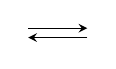
\begin{tikzpicture}[baseline] \draw[>=stealth,->] (0,1ex) -- (0.75,1ex); \draw[>=stealth,->] (0.75,0.25ex) -- (0,0.25ex); \end{tikzpicture}\ {#3}\thinspace\colon{#4}}

\renewcommand{\th}{\textsuperscript{th}}
\newcommand{\st}{\textsuperscript{st}}
\newcommand{\nd}{\textsuperscript{nd}}
\def\Cech{\v{C}ech}

% from http://tex.stackexchange.com/questions/41186/big-asterisk-bigast-symbol
% these are magic numbers that depend upon the other geometry options
\newcommand{\bigast}{\mathop{\scalebox{2.5}{\raisebox{-0.35ex}{$\ast$}}}}

% cf http://tex.stackexchange.com/questions/286050/rotated-math-with-correct-font-size for sizing instructions
\newcommand{\circulatearrows}{\text{$\curvearrowleft$\hspace{-0.90em}\rotatebox[origin=bl]{180}{$\curvearrowleft$}}}

\newcommand{\context}[1]{\mathcal{M}_{#1}}
\newcommand{\Ucontext}[1]{\mathcal{UM}_{#1}}
\newcommand{\Econtext}[1]{E_\infty\mathcal{M}_{#1}}
\newcommand{\CatOf}[1]{\normalfont\textsc{#1}}
\newcommand{\ps}[1]{\llbracket{#1}\rrbracket}
\newcommand{\moduli}[1]{\mathcal{M}_{\mathbf{#1}}}
\newcommand{\OS}[2]{\underline{\smash{#1}}_{#2}}
\newcommand{\InternalHom}[1]{\operatorname{\underline{\smash{\CatOf{#1}}}}}
\newcommand{\InternalAut}{\operatorname{\underline{\smash{\operatorname{Aut}}}}}
\newcommand{\InternalEnd}{\operatorname{\underline{\smash{\operatorname{End}}}}}
\newcommand{\sheaf}[1]{\mathcal{#1}}
\newcommand{\stack}[1]{\mathcal{#1}}
\newcommand{\ThomSheaf}[1]{\mathbb{L}(#1)}

\newcommand{\SO}{\mathit{SO}}
\newcommand{\SU}{\mathit{SU}}
\newcommand{\Spin}{\mathit{Spin}}
\newcommand{\String}{\mathit{String}}
\newcommand{\TMF}{\mathit{TMF}}
\newcommand{\Tmf}{\mathit{Tmf}}
\newcommand{\tmf}{\mathit{tmf}}
\renewcommand{\top}{\mathrm{top}}
\renewcommand{\ss}{\mathrm{ss}}
\newcommand{\ord}{\mathrm{ord}}
\newcommand{\alg}{\mathrm{alg}}
\renewcommand{\ns}{\mathrm{ns}}
\newcommand{\TAF}{\mathit{TAF}}
\newcommand{\BP}{\mathit{BP}}
\newcommand{\MU}{\mathit{MU}}
\newcommand{\Tate}{\mathrm{Tate}}
\newcommand{\gl}{\mathit{gl}}
\newcommand{\GL}{\mathit{GL}}
\newcommand{\perf}{\mathrm{perf}}
\newcommand{\gpd}{\mathrm{gpd}}
\newcommand{\ptyp}{p\text{-}\mathrm{typ}}
\newcommand{\id}{\mathrm{id}}
\newcommand{\FGps}{\mathrm{FGps}}
\newcommand{\fin}{\mathrm{fin}}
\newcommand{\Res}{\mathrm{Res}}
\newcommand{\Tr}{\mathrm{Tr}}
\newcommand{\Cart}{\mathrm{Cart}}
\newcommand{\tr}{\mathrm{tr}}
\newcommand{\spin}{\mathit{spin}}
\newcommand{\EinftyRings}{E_\infty\CatOf{RingSpectra}}

\DeclareMathOperator{\im}{im}
\DeclareMathOperator{\Ind}{Ind}
\DeclareMathOperator{\Spec}{Spec}
\DeclareMathOperator{\Spf}{Spf}
\DeclareMathOperator{\Sch}{Sch}
\DeclareMathOperator*{\colim}{colim}
\DeclareMathOperator{\End}{End}
\DeclareMathOperator{\Div}{Div}
\DeclareMathOperator{\SDiv}{SDiv}
\DeclareMathOperator{\Sq}{Sq}
\DeclareMathOperator{\Sym}{Sym}
\DeclareMathOperator{\Aut}{Aut}
\DeclareMathOperator{\Def}{Def}
\DeclareMathOperator{\Pic}{Pic}
\DeclareMathOperator{\Ext}{Ext}
\DeclareMathOperator{\hAut}{hAut}
\DeclareMathOperator{\Coord}{Coord}
\DeclareMathOperator{\Tor}{Tor}
\DeclareMathOperator{\Cotor}{Cotor}
\DeclareMathOperator{\coker}{coker}
\DeclareMathOperator{\Hom}{Hom}
\DeclareMathOperator{\Weil}{Weil}
\DeclareMathOperator{\Alt}{Alt}
\DeclareMathOperator{\Tot}{Tot}
\DeclareMathOperator{\height}{ht}
\DeclareMathOperator{\Sub}{Sub}
\DeclareMathOperator{\Level}{Level}
\DeclareMathOperator{\Mono}{Mono}
\DeclareMathOperator{\Isog}{Isog}
\DeclareMathOperator{\Td}{Td}
\DeclareMathOperator{\cofib}{cofib}
\DeclareMathOperator{\SpH}{SpH}
\DeclareMathOperator{\Lie}{Lie}
\DeclareMathOperator{\Frob}{Frob}
\let\div\undefined\DeclareMathOperator{\div}{div}

% theorem environments

% \numberwithin{equation}{section}

\theoremstyle{plain}
\newtheorem{theorem}{Theorem}[section]
\newtheorem{proposition}[theorem]{Proposition}
\newtheorem{lemma}[theorem]{Lemma}
\newtheorem{corollary}[theorem]{Corollary}
\newtheorem{conjecture}[theorem]{Conjecture}
\theoremstyle{definition}
\newtheorem{definition}[theorem]{Definition}
\newtheorem{construction}[theorem]{Construction}
\newtheorem{warning}[theorem]{Important Warning}
\theoremstyle{remark}
\newtheorem{remark}[theorem]{Remark}
\newtheorem{example}[theorem]{Example}

% sseqpages definitions

\sseqnewgroup\tower[1]{
    \class(0,0)
    \foreach \y in {2,...,#1} {
        \class(0, \y-1)
        \structline(0, \y-2, -1)(0, \y-1, -1)
    }
}

\sseqnewcmd\etaclass{
    \class[class labels=above left,\options](\x,\y)
    \structline(\x-1,\y-1,-1)(\x,\y,-1)
}

% section headers

\crefname{section}{lecture}{lectures} \Crefname{section}{Lecture}{Lectures}
\crefname{chapter}{case study}{case studies} \Crefname{chapter}{Case Study}{Case Studies}

% put commas between adjacent footnotes without disturbing hyperref

\let\oldFootnote\footnote
\newcommand\nextToken\relax

\renewcommand\footnote[1]{%
    \oldFootnote{#1}\futurelet\nextToken\isFootnote}

\newcommand\isFootnote{%
    \ifx\footnote\nextToken\textsuperscript{,}%
    \else\ifx\footnotemark\nextToken\textsuperscript{,}\fi%
    \fi}

% from hood chatham: an \HFp macro that deals with subsequent subscripts intelligently

\makeatletter
\protected\def\HFp{H\mathbb{F}_p\@ifnextchar_{{}}{}}
\protected\def\HFtwo{H\mathbb{F}_2\@ifnextchar_{{}}{}}
\makeatother

% from hood chatham: place relevant spectral sequences on verso-recto pairs

\usepackage{afterpage}
\def\afterrectopage#1{\afterpage{\ifodd\thepage #1\else\afterpage{#1}\fi}}

% from hood chatham: an \intertext command that works in tikzcd

% \usepackage{geometry}
\makeatletter
\edef\Gm@rmargin{\the\dimexpr1in + \hoffset + \evensidemargin}
\edef\Gm@lmargin{\the\dimexpr1in + \hoffset + \oddsidemargin}
\makeatother
\RequirePackage{tikz-cd}
\RequirePackage{etoolbox}

\usetikzlibrary{calc}
\edef\mytikzcdrestoreat{\catcode`@=\the\catcode`@\let\noexpand\mytikzcdrestoreat\noexpand\undefined}
\makeatletter
\newbox\mytikzcd@trialbox

\patchcmd\tikzcd@{#1]}{remember picture,#1]\let\intertext\mytikzcd@intertext}{}{\errorfailedtopatch}



\def\mytikzcd@addtosavedpaths#1{\xdef\tikzcd@savedpaths{\unexpanded\expandafter{\tikzcd@savedpaths}#1}}
\def\mytikzcd@intertext{
	\@ifnextchar[{\mytikzcd@intertext@}{\mytikzcd@intertext@[0pt]}
}

\def\mytikzcd@intertext@[#1]#2{
	\setbox\mytikzcd@trialbox=\vbox{\hsize\textwidth #2}
	\expandafter\\\expandafter[\the\dimexpr\ht\mytikzcd@trialbox+\dp\mytikzcd@trialbox+#1]
    \edef\mytikzcd@lmargin{\if@mparswitch\ifodd\thepage\space \Gm@lmargin\else \Gm@rmargin\fi\else \Gm@lmargin\fi}
    \@xp\mytikzcd@findcolumn\@xp{\tikzcd@savedpaths}{1}
	\mytikzcd@addtosavedpaths{\unexpanded{\path[overlay] let \p1=(current page.west), \p2 =} (\noexpand\tikzcdmatrixname-\the\numexpr\pgfmatrixcurrentrow-1\relax-\mytikzcd@column), \noexpand\p3 = (\noexpand\tikzcdmatrixname-\the\pgfmatrixcurrentrow-1) in
	node[anchor=west,xshift=\mytikzcd@lmargin-2pt] at \unexpanded{(\x1,0.5*\y2+0.5*\y3) {\parbox{\textwidth}{#2}};}
	}
}


\def\mytikzcd@findcolumn#1#2{
    \def\mytikzcd@targetrow{#2}
    \expandafter\mytikzcd@findcolumn@\detokenize{#1\def\tikzcd@currentcolumn{x}\def\tikzcd@currentrow{6}}\@nil
}
\bgroup\lccode`\(=`\{\lccode`\)=`\}\lowercase{\egroup
\edef\mytikzcd@findcolumn@argspec{\unexpanded{#1}\detokenize{\def\tikzcd@currentcolumn}\unexpanded{(#2)}\detokenize{\def\tikzcd@currentrow}\unexpanded{(#3)}}
}

\@xp\def\@xp\mytikzcd@findcolumn@\mytikzcd@findcolumn@argspec{
    \expandafter\ifx\detokenize{x}#2
        \ifnum\mytikzcd@row<\the\numexpr\pgfmatrixcurrentrow-1\relax\def\mytikzcd@column{1}\fi
        \@xp\@gobbletonil
    \else
        \def\mytikzcd@column{#2}
        \def\mytikzcd@row{#3}
        \@xp\mytikzcd@findcolumn@
    \fi
}



\def\@gobbletonil#1\@nil{}
\mytikzcdrestoreat 

% from hood chatham: 

% taken from https://tex.stackexchange.com/a/164490/2671

\makeatletter
\newcommand{\sumfgl}[1]{\mathop{\vphantom{\sum}\mathpalette\sum@fgl{#1}}}
\newcommand{\sum@fgl}[2]{%
  \ooalign{%
    \sum@fgl@vc{#1}{\sum}\cr
    \hidewidth\sum@fgl@vc{\sum@fgl@next{#1}}{\mkern17mu#2}\hidewidth\cr}%
}
\newcommand{\sum@fgl@vc}[2]{%
  $\vcenter{\hbox{$\m@th#1#2$}}$%
}
\newcommand{\sum@fgl@next}[1]{%
  \ifx#1\displaystyle\scriptstyle\fi
  \ifx#1\textstyle\scriptscriptstyle\fi
  \ifx#1\scriptstyle\scriptscriptstyle\fi
  \ifx#1\scriptscriptstyle\scriptscriptstyle\fi
}
\def\sumphi{\sumfgl{\phi}}
\def\sumG{\sumfgl{\G}}
\def\sumGamma{\sumfgl{\Gamma}}
\makeatother




% from https://tex.stackexchange.com/questions/52076/how-to-make-a-superscript-on-the-upper-left-hand-corner-of-a-letter :

\def\presuper#1#2%
  {\mathop{}%
   \mathopen{\vphantom{#2}}^{#1}%
   \kern-\scriptspace%
   #2}

% from hood chatham: 
\makeatletter
\def\idxentry{\@ifnextchar[{\idxentry@}{\idxentry@dbl}}
% \def\idxentry@dbl#1{\mycommand@[#1]{#1}}
\def\idxentry@dbl#1{\textit{#1}\index{#1}}
\def\idxentry@[#1]#2{\textit{#2}\index{#1@#2}}
\makeatother

% from hood chatham: fix cleveref to work with cambridge7a
\makeatletter
\AtBeginDocument{%
\def\@thm{\@ifnextchar[{\cref@thmoptarg}{\cref@thmnoarg}}%]
\patchcmd\cref@thmoptarg {.}{\enskip}{}{\error}}
\makeatother

\makeatletter
\AtBeginDocument{%
\patchcmd{\@makechapterhead}{\huge\bfseries \thechapter}{\huge\bfseries \chaptername\ \thechapter}{}{\error}%
}
\makeatother

% set the default arrow style
\tikzset{>=stealth}
\tikzcdset{arrow style=tikz}

% put rectos back into \chapter
\makeatletter
\patchcmd{\chapter}{\clearpage}{\cleardoublepage}{}{\error}
\makeatother

% make backrefs look pretty
\renewcommand*{\backref}[1]{}
\renewcommand*{\backrefalt}[4]{[%
    \ifcase #1 Not cited.%
          \or Cited on page~#2.%
          \else Cited on pages #2.%
    \fi%
    ]}

\allowdisplaybreaks

%%% Created by texsupport 20/09/2017

\makeatletter
\ifAJW@confsty
%
  \def\appendix{%
    \apptmp=\c@chapter %save chapter number
    \par
    \AJW@appendixtrue
    \def\section{\@startsection {section}{1}{\z@}
      {-30\p@ \@plus-7\p@ \@minus-3.5\p@}{8\p@}{\Aheadsize\bfseries\centering Appendix~}}
    \setcounter{section}{0}
    \@addtoreset{figure}{subsection}
    \setcounter{figure}{0}
    \setcounter{table}{0}
% set tocdepth to chapter heads only whether multi-author or single-author
    %\addtocontents{toc}{\protect\setcounter{tocdepth}{1}}
    \def\@chapapp{\appendixname}
    \def\thechapter {\Alph{chapter}}
    \def\thesection {\Alph{section}}
    \def\thesubsection {\Alph{section}.\arabic{subsection}}
    \def\thetable   {\Alph{section}.\@arabic\c@table}
    \def\thefigure  {\Alph{section}.\@arabic\c@figure}
    \def\theequation{\Alph{section}.\arabic{equation}}
}

% and only one appendix
  \def\oneappendix{\AJW@oneappendixtrue\appendix
    \def\thesection {}% remove the 'A' from Appendix heading
  }
\else
%
% single version
\def\appendix{\par\clearpage
 \AJW@appendixtrue
 \setcounter{chapter}{0}
 \setcounter{section}{0}
% set tocdepth to chapter heads only whether multi-author or single-author
 %\addtocontents{toc}{\protect\setcounter{tocdepth}{0}}
 \def\@chapapp{\appendixname}
 \def\thechapter {\Alph{chapter}}
 \def\thesection {\thechapter.\arabic{section}}
 \def\thetable   {\thechapter.\@arabic\c@table}
 \def\thefigure  {\thechapter.\@arabic\c@figure}
 \def\theequation{\thechapter.\arabic{equation}}
}
%
% and only one appendix
    \def\oneappendix{\AJW@oneappendixtrue\appendix}
\fi

\makeatother



% if these change, be sure to update the pdf metadata in preamble.tex
\title{Formal Geometry and Bordism Operations \\ \vspace{0.5\baselineskip} \small{Lecture notes}}
\author{Eric Peterson}
\date{{\footnotesize Compiled: \today \\ Git hash: {\gitAbbrevHash}{\gitDirty}}}




% --- REMOVE ME EVENTUALLY ---

\let\oldTodo\todo
\newcounter{todocounter}
\setcounter{todocounter}{0}
\renewcommand{\todo}{\addtocounter{todocounter}{1}\oldTodo}

% --- END REMOVE ME EVENTUALLY ---





\begin{document}

\frontmatter

\maketitle

% -*- root: main.tex -*-

% \input{class-info}

\cleardoublepage

\vspace*{\fill}

\begin{center}
``Let us be glad we don't work in algebraic geometry.''

\hspace{6.3em} ------J.\ F.\ Adams~\cite[Section 2.1]{AdamsInfiniteLoopSpaces}
\end{center}

\vspace*{\fill}

\cleardoublepage

% -*- root: main.tex -*-

\subsection*{Foreword (Matthew Ando)}

This book does a remarkable job of introducing some of the 
interaction between algebraic topology and algebraic geometry, which
these days---thanks to Doug Ravenel---goes by the name ``chromatic
stable homotopy theory.''

Chromatic homotopy theory had its origins in the work of Novikov and
Quillen, who first investigated the relationship between complex
cobordism and formal groups and perceived its potential for
investigating the stable homotopy groups of spheres. That this works
as well as it does still boggles my mind, and there is still research
to be done to understand why this is so (for example the recent work
of Beardsley, mentioned in the Appendix).  

We are fortunate that Jack Morava perceived that the work of Novikov
and Quillen hinted at a deep relationship between the structure of
the stable category and the structure of the stack of formal groups,
and that he was persuasive enough to get others including Landweber,
Miller, Ravenel, and Wilson excited about this approach. The
remarkable activity that followed culminated in  Ravenel's periodicity
conjectures and their resolution by Devinatz, Hopkins, and Smith. 

The chromatic homotopy theorists of the 1970s took Morava's
vision as inspiration and proved amazing results, but in their
published work they usually did not make use of modern
algebro-geometric methods, such as the theory of stacks, which was
more or less simultaneously under development.  (Although in
``Forms of $K$-theory''~\cite{MoravaFormsOfKthy}, which dates as far back as 1973, Morava sketches
a stacky proof of Landweber's exact functor theorem.)

Around 1990, the study of chromatic stable homotopy underwent a
qualitative change. Mike Hopkins took the lead in
showing that algebraic geometry and the theory of stacks
provide powerful tools for proving theorems in chromatic homotopy
theory; at the same time, the conceptual picture of the subject became
much simpler.  The simplifications that resulted made it possible for
many more people, including me, to enter the subject. 

I was fortunate to have Haynes Miller and Mike Hopkins as
teachers.  I was also fortunate to have Adams's ``blue book''~\cite{AdamsBlueBook} and
Ravenel's ``green book''~\cite{RavenelGreenBook}. Until recently, students entering the
subject since the 1990's have not had access to comparable sources
which introduce them to the mix of algebraic topology and algebraic
geometry which form the context for  
modern chromatic stable homotopy theory (although Strickland's 
lovely 
``Formal Schemes and Formal Groups''~\cite{StricklandFSFG} is a notable exception).  This has
begun to change, and there are several expositions of aspects of the
subject---the list in the acknowledgements of this volume are a good
starting point.  

This brings me to this book.  I had the good fortune to meet
Eric as an undergraduate and convince him to work on some problems I
was interested in. The things that make Eric fun to work with are
well reflected in this book.  It has a down-to-earth and inviting
style (no small achievement in a book about 
functorial algebraic geometry).  It is elegant,
precise, and incisive, and it is strong on both theory and
calculation.  An important feature of the book is that it takes the
time to give elegant proofs of some ``theory-external'' results:
theorems you might care about even if chromatic stable homotopy theory isn't
your subject.  

There is a huge amount yet to be discovered: the Appendix indicates
some possible directions for future research.  It is great to see this
material assembled here to help the next generation of researchers get
started on an exciting subject.

\vspace{2\baselineskip}
\hspace{3em} ------------Matthew Ando

\hspace{7em} October 2\textsuperscript{nd}, 2017


\cleardoublepage

\subsection*{Acknowledgements}


This book owes an incredible amount to an incredible number of incredible people.  Understanding the research program summarized here has been one of the primary pursuits---if not \emph{the} primary pursuit---of my young academic career.  It has been an unmistakable and enormous privilege not only to be granted the time and freedom to learn about these beautiful ideas, but to also be able to do so directly from their progenitors.  I owe very large debts to Matthew Ando, Michael Hopkins, and Neil Strickland, for each having shown me such individual attention and care, as well as for having worked out the tail of this long story.  Matt, in particular, is the person who got me into higher mathematics, and I feel that for a decade now I have been paying forward the good will and deep friendliness that he showed me during my time at Urbana--Champaign.  Mike and Neil are not far behind.  Mike has been my supervisor in one sense or another for years running, in which role he has been continually encouraging and giving.  Among other things, Neil shared with me a note of his that eventually blossomed into my thesis problem, which is an awfully nice gift to have given.

Less directly in ideas but no less directly in stewardship, I also owe a very large debt to my Ph.D.\ adviser, Constantin Teleman.  By the time I arrived at UC--Berkeley, I was already too soaked through with homotopy theory to develop a flavor for his sort of mathematical physics, and he nonetheless endeavored to meet me where I was.  It was Constantin who encouraged me to put special attention into making these ideas accessible, speaking understandably, and highlighting the connections with nearby fields.  He emphasized that mathematics done in isolation, rather than in maximal connection to other people, is mathematics wasted.  He has very much contributed to my passion for communication and clarity, which---in addition to the literal mathematics presented here---is the main goal of this text.\footnote{I have a clear memory of delivering a grad student seminar talk during my first year, where my mathematical sibling, George Melvin, asked me why $\G_m$ was called the multiplicative formal group.  I looked at him, looked at the board, and cautiously offered, ``\ldots because of the mixed term in the group law?''  Silly as it seems, this book has been shaped in no small way by striving to correct for this single highly inarticulate incident, where it was revealed that I did not understand the original context of these tools that topologists were borrowing.  Although everyone starts learning from somewhere and not-knowing something is no cause for lasting embarrassment, it is certainly still helpful to receive pushes in the direction of intellectual responsibility.  Thanks, George.}\footnote{It is, of course, up to the reader to determine whether I have actually succeeded at this, and, of course, any failure of mine in this regard can't possibly be visited upon Constantin.}

More broadly, the topology community has been very supportive of me as I have learned about, digested, and sometimes erroneously recapitulated the ideas of chromatic homotopy theory, tolerating me as a very loud and public learner.  Haynes Miller, Doug Ravenel, and Steve Wilson (the $BP$ Mafia~\cite{HopkinsOnRavenel}) have all been invaluable resources: they have answered my questions tirelessly, they are each charming and friendly, they are prolific and meticulous authors, and they literally invented this subfield of mathematics.  Jack Morava has played no smaller a role in both the discovery of chromatic homotopy theory and my own personal education.  It has been an incredible treat to know him and to have received pushes from him at critical moments.  Nat Stapleton and Charles Rezk also deserve special mention: power operations were among the last things that I managed to understand while writing this book, and it is an enormous credit first to their intelligence that they are so comfortable with something so bottomlessly complicated and second to their inexhaustible patience that they walked me through understanding this material time and time again, in the hopes that I would someday get it.

The bulk of this book began as a set of lecture notes for a topics course\footnote{MATH 278 (159627), Spring 2016.} that I was invited to teach at Harvard University in the spring term of 2016, and I would like to thank the department for the opportunity and for the very enriching time that I spent there.  The \emph{germ} of these notes, however, took root at the workshop \textit{Flavors of Cohomology}, organized and hosted by Hisham Sati in June 2015.  In particular, this was the first time that I tried to push the idea of a ``context'' on someone else, which---for better or worse---has grown into the backbone of this book.  The book also draws on feedback from lecturing in the \textit{In-Formal Groups Seminar}, which took place during the MSRI semester program in homotopy theory in the spring term of 2014, attended primarily by David Carchedi, Achim Krause, Matthew Pancia, and Sean Tilson.  Finally, my thoughts about the material in this book and its presentation were further refined by many, many, \emph{many} conversations with other students at UC--Berkeley, primarily: my undergraduate readers Hood Chatham and Geoffrey Lee, the visiting student Catherine Ray, and my officemates Aaron Mazel-Gee and Kevin Wray---who, poor guys, put up with listening to me for years on end.

This book also draws on a lot of unpublished material.  The topology community gets some flak for this reluctance to publish certain documents, but I think it is to our credit that they are made available anyway, essentially without redaction.  Reference materials of this sort which have influenced this book include: Matthew Ando's \textit{Dieudonn\'e Crystals Associated to Lubin--Tate Formal Groups}; Michael Hopkins's \textit{Complex Oriented Cohomology Theories and the Language of Stacks}; Jacob Lurie's \textit{Chromatic Homotopy (252x)}; Haynes Miller's \textit{Notes on Cobordism}; Charles Rezk's \textit{Elliptic Cohomology and Elliptic Curves}, as well as his \textit{Notes on the Hopkins--Miller Theorem}, and his \textit{Supplementary Notes for Math 512}; Neil Strickland's \textit{Formal Schemes for $K$--Theory Spaces} as well as his \textit{Functorial Philosophy for Formal Phenomena}; the Hopf archive preprint version of the Ando--Hopkins--Strickland article \textit{Elliptic Spectra, the Witten Genus, and the Theorem of the Cube}\footnote{This earlier version contains a lot of information that didn't make it to publication, as the referee (perhaps rightly) found it too dense to make heads or tails of.  Once the reader already has the sketch of the argument established, however, the original version is a truly invaluable resource to go back and re-read.}; and the unpublished Ando--Hopkins--Strickland article \textit{Elliptic Cohomology of $BO\<8\>$ in Positive Characteristic}, recovered from the mists of time by Gerd Laures\footnote{There is a bit of a funny story here: none of the authors of this article could find their own preprint, but one of their old graduate students had held on to a paper copy.  In their defense, two decades had passed---but that in turn only makes Gerd's organizational skills more heroic.}.  I would not have understood the material presented here without access to these resources, nevermind the supplementary guidance.

In addition to their inquisitive presences in the lecture hall, the students who took the Harvard topics course under me often contributed directly to the notes.  These contributors are: Eva Belmont, Hood Chatham (especially his marvelous spectral sequence package, \texttt{spectralsequences}), Dexter Chua (an outside consultant who translated the picture in \Cref{MfgPicture} from a scribble on a scrap of paper into something of professional caliber, who provided a mountain of valuable feedback, and who came up with the book's clever epigraph), Arun Debray (a student at UT--Austin), Jun Hou Fung, Jeremy Hahn (especially the material in \Cref{ComplexBordismChapter} and \Cref{JuvitopTalkSection}), Mauro Porta, Krishanu Sankar, Danny Shi, and Allen Yuan (especially, again, \Cref{JuvitopTalkSection}, which I might have never tried to understand without his insistence that I speak about it and his further help in preparing that talk).

More broadly, the following people contributed to the course just by attending, where I have highlighted those who additionally survived to the end of the semester: Colin Aitken, Adam Al-Natsheh, \textbf{Eva Belmont}, Jason Bland, Dorin Boger, \textbf{Lukas Brantner}, \textbf{Christian Carrick}, \textbf{Hood Chatham}, David Corwin, \textbf{Jun Hou Fung}, \textbf{Meng Guo}, \textbf{Jeremy Hahn}, Changho Han, Chi-Yun Hsu, \textbf{Erick Knight}, Benjamin Landon, Gabriel Long, Yusheng Luo, Jake Marcinek, \textbf{Jake McNamara}, \textbf{Akhil Mathew}, Max Menzies, Morgan Opie, Alexander Perry, Mauro Porta, \textbf{Krishanu Sankar}, \textbf{Jay Shah}, Ananth Shankar, \textbf{Danny Shi}, Koji Shimizu, Geoffrey Smith, Hunter Spinik, Philip Tynan, Yi Xie, David Yang, Zijian Yao, Lynnelle Ye, Chenglong Yu, \textbf{Allen Yuan}, Adrian Zahariuc, Yifei Zhao, Rong Zhou, and Yihang Zhu.  Their energy and enthusiasm were overwhelming---I felt duty-bound to keep telling them things they didn't already know, and despite my best efforts to keep out ahead I also felt like they were constantly nipping at my heels.  As I've gone through my notes during the editing process, it has been astonishing to see how reliably they asked exactly the right question at exactly the right time, often despite my own confusion.  They're a \emph{very} bright group.  Of the highlighted names, Erick Knight deserves special mention: he was an arithmetic geometer living among the rest of us topologists, and he attentively listened to me butcher his native field without once making me feel self-conscious.\footnote{Between him and Dorin, I do wonder if there's a Fossey-esque novel in the works: \textit{Topologists in the Mists}.  I hope our impression was as gentle creatures, uncannily similar to proper mathematicians once you get to know us.}

On top of the students, various others have contributed in this way or that during the long production of this book, from repairing typos to long conversations and between.  Such helpful people include: Tobias Barthel, Jonathan Beardsley, Martin Bendersky, Sanath Devalapurkar, Ben Gadoua, Mike Hill, Johan Konter, Achim Krause, Akhil Mathew, Pedro Mendes de Araujo, Denis Nardin, Justin Noel, Sune Precht Reeh, Andrew Senger, Reuben Stern, Sean Tilson, and Dylan Wilson.  Of course, Matt Ando, Mike Hopkins, and Nat Stapleton deserve further special mention as direct contributors of their respective sections.  Additionally, the referees and the publishers themselves have been enormously helpful in editing this into a passable document.

Lastly, but by far most importantly, this book---and, frankly, \emph{I}---would not have made it out of the gates without Samrita Dhindsa's love, support, and patience.  She made living in Boston a completely different experience: a balanced life instead of being quickly and totally overwhelmed by work, a lively circle of friends instead of what would have been a much smaller world, new experiences instead of worn-through ones, and love throughout.  Without her compassion, tenderness, and understanding I would not be half the open and vibrant person that I am today, and I would know so much less of myself.  It is awe-inspiring to think about, and it is a pleasure and an honor to acknowledge her like this and to dedicate this book to her.

Thanks to my many friends here, and thanks also to Thomas Dunning especially.  Thanks, everyone.  Theveryone.

\vspace{2\baselineskip}
\hspace{3em} ------------Eric



\newpage
\tableofcontents

\todo[inline]{I would like as few section titles as possible to involve people's names.}
\todo[inline]{A bunch of broken displaymode tombstones can have their positions fixed by using http://tex.stackexchange.com/a/66221/2671.}
\todo[inline]{Compile an index by replacing all the \texttt{textit} commands in definition environments with some more fancy macro that tags it for inclusion.  There's information on how indices are compiled here: https://en.wikibooks.org/wiki/LaTeX/Indexing.}
\todo[inline]{Remember to use $f\co A \to B$ everywhere.}
\todo[inline]{Should sections have subsections?  Does that help organize the TOC?}
\todo[inline]{Hood wrote a macro called sumfgl (see also sumF and sumG) that will make a bunch of formal group law expressions typeset better. Propagate that change through.  Consider also the adjunct macro in the preamble.  (Jay says that left-adjoints should be on top in general.)}
\todo[inline]{Make sure you use either $\id$ or $1$ everywhere to denote the identity morphism.}
\todo[inline]{You're not very consistent about using $\G$ or $\Gamma$ to denote an arbitrary formal group. It seems like you use one or the other based on your preference of whether it has finite height or not.}
\todo[inline]{Eliminate contractions.}
\todo[inline]{Eliminate filler words like ``things''.}
\todo[inline]{Make sure that ``Case Study'' and ``Lecture'' are OK names by the publisher's standards. If they aren't, do a careful search-and-replace for them.}
\todo[inline]{Double check that you're careful about choosing consistent names for your objects: $S = \Spec R$ is the base scheme, that sort of thing.}
\todo[inline]{Be consistent about $\sheaf O_X$ vs $\sheaf O(X)$, and similarly with $\sheaf I_D$ versus $\sheaf I(D)$.}
\todo[inline]{Be consistent about ``$\S$'' versus ``$\S^0$'' for the standard sphere spectrum.}
\todo[inline]{The AGT style guide says that ``---'' should not have spaces on either side.}
\todo[inline]{We should use the convention that $\phi \in \moduli{fgl}(T)$ corresponds to $x +_\phi y \in T\ps{x, y}$ throughout.}
\todo[inline]{Jon suggested that we include backreferences from the bibliography, using the package \texttt{backref}.  More information on getting this to work well is at this tex.se url: http://tex.stackexchange.com/questions/54541/precise-back-reference-target-with-hyperref-and-backref .}
\todo[inline]{Use Hood's HFp macro where appropriate.  (Maybe modify it also to do HF2 appropriately.)  (Maybe also modify it to use upright $\mathrm{H}$?  Sean thinks that ital $H$ next to blackboard bold (and upright) $\F$ looks bad.)}
\todo[inline]{Clark's use of MinionPro font is really nice (cf. \texttt{https://dl.dropboxusercontent.com/u/1741495/teaching/2017spring.18.917/gamma-blurb.pdf}).  Generally, we should make an effort to pick a nice font.  http://web.willbenton.com/writing/2008/better-latex has more info about converting FF fonts for use in LaTeX, including Minion.}
\todo[inline]{Use booktabs (http://www.ctan.org/tex-archive/macros/latex/contrib/booktabs/) to typeset any tables appearing in this book.  (I don't think there are very many.)}
\todo[inline]{In several places you abuse the \texttt{align*} environment to put references into a right-hand column.  Is there a less hack-y way to do this?}
\todo[inline]{Be consistent about hyphens / en-dashes connecting ``$A$/$E$/$H_\infty$'' to ``ring''.}
\todo[inline]{Consider adding chapter epigraphs? Maybe from The Ninth Gate?}
\todo[inline]{Use $\EinftyRings$ everywhere appropriate.}




\mainmatter

% -*- root: main.tex -*-

\setcounter{chapter}{-1}
\chapter{Introduction}

\label{IntroductionSection}

The goal of this book is to communicate a certain \textit{Weltanschauung} uncovered in pieces by many different people working in bordism theory, and the goal just for this introduction is to tell a story about one theorem where it is especially apparent.

To begin, we will define a homology theory called \index{bordism!geometric chains}\textit{bordism homology}.  Recall that the singular homology of a space \(X\) comes about by probing \(X\) with simplices: beginning with the collection of continuous maps \(\sigma\co \Delta^n \to X\), we take the free \(\Z\)--module on each of these sets and construct a chain complex \[\cdots \xrightarrow{\partial} \Z\{\Delta^n \to X\} \xrightarrow{\partial} \Z\{\Delta^{n-1} \to X\} \xrightarrow{\partial} \cdots.\]  Bordism homology is constructed analogously, but using manifolds \(Z\) as the probes instead of simplices:\footnote{One does not need to take the free abelian group on anything, since the disjoint union of two manifolds is already a (disconnected) manifold, whereas the disjoint union of two simplices is not a simplex.}
\begin{align*}
\cdots & \xrightarrow{\partial} \{Z^n \to X \mid \text{\(Z^n\) a compact \(n\)--manifold}\} \\
& \xrightarrow{\partial} \{Z^{n-1} \to X \mid \text{\(Z^{n-1}\) a compact \((n-1)\)--manifold}\} \\
& \xrightarrow{\partial} \cdots.
\end{align*}

\begin{lemma}[{\cite[Section 4]{Kochman}}]\label{OriginalDefnOfBordism}
This forms a chain complex of monoids under disjoint union of manifolds, and its homology is written \(MO_*(X)\).  These are naturally abelian groups\footnote{For instance, the inverse map comes from the cylinder construction: for a manifold \(M\), the two components of \(\partial(I \times M)\) witness the existence of an inverse to \(M\) in the bordism groups.}, and moreover they satisfy the axioms of a generalized homology theory. \qed
\end{lemma}

In fact, we can define a bordism theory \(MG\) for any suitable family of structure groups \(G(n) \to O(n)\).  The coefficient ring of \(MG\), or its value \(MG_*(*)\) on a point, gives the ring of \(G\)--bordism classes, and generally \(MG_*(Y)\) gives a kind of ``bordism in families over the space \(Y\)''.  There are comparison morphisms for the most ordinary kinds of bordism, given by replacing a chain of manifolds with an equivalent simplicial chain:
\begin{align*}
MO & \to H\Z/2, &
M\SO & \to H\Z. \\
\intertext{In both cases, we can evaluate on a point to get ring maps, called \index{orientation!genus}\textit{genera}:}
MO_*(*) & \to \Z/2, &
M\SO_*(*) & \to \Z,
\end{align*}
neither of which is very interesting, since they are both zero in positive degrees.

However, having maps of homology theories (or, really, of spectra) is considerably more data than just the genus.  For instance, we can use such a map to extract a theory of integration by considering the following special case of oriented bordism, where we evaluate \(M\SO_*\) on an infinite loopspace:
\begin{align*}
M\SO_n K(\Z, n) & = \left\{ \text{oriented \(n\)--manifolds mapping to \(K(\Z, n)\)} \right\} / \sim \\
& = \left. \left\{ \begin{array}{c}\text{oriented \(n\)--manifolds \(Z\)} \\ \text{with a specified class \(\omega \in H^n(Z; \Z)\)} \end{array}\right\} \middle/ \sim \right. .
\end{align*}
Associated to such a representative \((Z, \omega)\), the yoga of stable homotopy theory then allows us to build a composite
\begin{align*}
\S & \xrightarrow{\mathmakebox[2.5em]{(Z, \omega)}} M\SO \sm (\S^{-n} \sm \Susp^\infty_+ K(\Z, n)) \\ 
& \xrightarrow{\mathmakebox[2.5em]{\colim}} M\SO \sm H\Z \\
& \xrightarrow{\mathmakebox[2.5em]{\phi \sm 1}} H\Z \sm H\Z \\
& \xrightarrow{\mathmakebox[2.5em]{\mu}} H\Z,
\end{align*}
where \(\phi\) is the orientation map.  Altogether, this composite gives us an element of \(\pi_0 H\Z\), i.e., an integer.%\todo{I used to think that we got a generalized Stokes's theorem too, but now I'm not sure. Stokes's theorem is the statement that the chain and cochain differentials are adjoint: \(\<d\omega, \sigma\> = \<\omega, \partial \sigma\>\), where the pairing is the integration pairing.  It would be neat to interpret this in generality, but it might be a stretch.}

\begin{lemma}%\citeme{Where is this proven?}
The integer obtained by the above process is \(\int_Z \omega\). \qed
\end{lemma}

\noindent Many theorems accompany this definition of \(\int_Z \omega\) for free, entailed by the general machinery of stable homotopy theory.  The definition is also very general: given a ring map off of any bordism spectrum, a similar sequence of steps will furnish us with an integral tailored to that situation.

Now take \(G = e\) to be the trivial structure group, which is the bordism theory of framed manifolds, i.e., those with stably trivial normal bundle.  In this case, the \index{Pontryagin--Thom construction}Pontryagin--Thom construction gives an equivalence \(\S \xrightarrow{\simeq} Me\).  It is thus possible that stable homotopy theory can be investigated solely through the lens of framed bordism.\footnote{Indeed, some people have taken up this viewpoint.  For a completely noncanonical point of entry, see Stolz~\cite{Stolz}.}  We will prefer to view this the other way: the sphere spectrum \(\S\) often appears to us as a natural object, and we will occasionally replace it by \(Me\), the framed bordism spectrum.  For example, given a ring spectrum \(E\) with unit map \(\S \to E\), we can reconsider this as a ring map \[Me \xrightarrow{\simeq} \S \to E.\]  Following along the lines of the previous paragraph, we learn that any ring spectrum \(E\) is automatically equipped with a theory of integration for framed manifolds.

Sometimes, as in the examples above, this unit map factors: \[\S \simeq Me \to MO \to H\Z/2.\]  This is a witness to the overdeterminacy of \(H\Z/2\)'s integral for framed bordism: if the framed manifold is pushed all the way down to an unoriented manifold, there is still enough residual data to define the integral.\footnote{It is literally more information than this: even unframeable unoriented manifolds acquire a compatible integral.}  Given any ring spectrum \(E\), we can ask the analogous question: If we filter \(O\) by a system of structure groups, through what stage does the unit map \(Me \to E\) factor?  For instance, the map \[\S = Me \to M\SO \to H\Z\] considered above does \emph{not} factor further through \(MO\)---an orientation is \emph{required} to define the integral of an integer--valued cohomology class.  Recognizing \(\SO \to O\) as the \(0\){\th} Postnikov--Whitehead truncation of \(O\), we are inspired to use the rest of the \index{Postnikov tower}Postnikov filtration as our filtration of structure groups.  Here is a diagram of this filtration and some interesting minimally-factored integration theories related to it, circa 1970:
\begin{center}
\begin{tikzcd}
Me \arrow{r} \arrow{rrrd} \arrow{rrrrd} \arrow{rrrrrd} & \cdots \arrow{r} & M\String \arrow{r} & M\Spin \arrow{r} \arrow[crossing over]{d} & M\SO \arrow{r} \arrow[crossing over]{d} & MO \arrow[crossing over]{d} \\
& & & kO & H\Z & H\Z/2.
\end{tikzcd}
\end{center}

This is the situation homotopy theorists found themselves in some decades ago, when Ochanine and Witten proved the following mysterious theorem using analytical and physical methods:

\begin{theorem}[{Ochanine~\cite{Ochanine,OchanineEnrichmentToKO}, Witten~\cite{WittenEllipticGeneraQFT,WittenIndexDiracOperatorLoopSpace}}]\label{OchanineWittenTheorem}\index{orientation!Witten genus}
There is a map of rings \[\sigma: M\Spin_* \to \C(\!(q)\!).\]  Moreover, if \(Z\) is a \(\Spin\) manifold such that half\footnote{It is a special property of \(\Spin\)--manifolds that this class is always divisible by \(2\).} its first Pontryagin class vanishes---that is, if \(Z\) lifts to a \(\String\)--manifold---then \(\sigma(Z)\) lands in the subring \(MF \subseteq \Z\ps{q}\) of \index{modular form!q expansion@\(q\)--expansion}\(q\)--expansions of \index{modular form}modular forms with integral coefficients. \qed
\end{theorem}

\noindent However, neither party gave indication that their result should be valid ``in families'' (in our sense), and no theory of integration was formally produced (in our sense).  From the perspective of the homotopy theorist, it was not even totally clear what such a claim would mean: to give a topological enrichment of these theorems would mean finding a ring spectrum \(E\) such that \(E_*(*)\) had something to do with modular forms.

Around the same time, Landweber, Ravenel, and Stong began studying \index{elliptic spectrum}\textit{elliptic cohomology} for independent reasons~\cite{LRS}; sometime much earlier, Morava had constructed an object ``\(K^{\Tate}\)'' associated to the \index{Tate curve}Tate elliptic curve~\cite[Section 5]{MoravaFormsOfKthy}; and a decade later Ando, Hopkins, and Strickland~\cite{AHSTheoremOfTheCube} put all these together in the following theorem:

\begin{theorem}[{\cite[Theorem 2.59]{AHSTheoremOfTheCube}}]
If \(E\) is an ``elliptic cohomology theory'', then there is a canonical map of homotopy ring spectra \(M\String \to E\) called the \index{sigma orientation@\(\sigma\)--orientation}\(\sigma\)--orientation (for \(E\)).  Additionally, there is an elliptic spectrum \(K^{\Tate}\) whose \(\sigma\)--orientation gives Witten's genus \(M\String_* \to K^{\Tate}_*\) . \qed
\end{theorem}

We now come to the motivation for this text: the homotopical \(\sigma\)--orientation was actually first constructed using formal geometry.  The original proof of Ando--Hopkins--Strickland begins with a reduction to maps of the form \[MU[6, \infty) \to E.\]  They then work to show that in especially good cases they can complete the missing arrow in the diagram
\begin{center}
\begin{tikzcd}
MU[6, \infty) \arrow{r} \arrow{rd} & M\String \arrow[densely dotted]{d} \\
& E.
\end{tikzcd}
\end{center}
Leaving aside the extension problem for the moment, their main theorem is the following description of the cohomology ring \(E^* MU[6, \infty)\):

\begin{theorem}[{Ando--Hopkins--Strickland~\cite{AHSTheoremOfTheCube}, cf.\ Singer~\cite{Singer} and Stong~\cite{Stong}}]\label{IntroAHSMU6Thm}
For \(E\) an even--periodic cohomology theory, there is an isomorphism \[\Spec E_* MU[6, \infty) \cong C^3(\G_E; \sheaf I(0)),\] where ``\(C^3(\G_E; \sheaf I(0))\)'' is the affine scheme parametrizing \index{cubical structure}\textit{cubical structures} on the line bundle \(\sheaf I(0)\) over \(\G_E\).  When \(E\) is taken to be elliptic, so that there is a specified \index{elliptic curve}elliptic curve \(C\) and a specified isomorphism \(\G_E \cong C^\wedge_0\), the theory of elliptic curves gives a canonical such cubical structure and hence a preferred class \(MU[6, \infty) \to E\).  This assignment is natural in the choice of elliptic \(E\). \qed
\end{theorem}

Our real goal is to understand theorems like this last one, where algebraic geometry asserts some real control over something squarely in the domain of homotopy theory, and we will work through a sequence of case studies where this perspective shines through most brightly.  In particular, rather than taking an optimal route to the Ando--Hopkins--Strickland result, we will use it as a gravitational slingshot to cover many anciliary topics which are also governed by the technology of formal geometry.  We will begin by working through Thom's calculation of the homotopy of \(MO\), which holds the simultaneous attractive features of being approachable while revealing essentially all of the structural complexity of the general situation, so that we know what to expect later on.  Having seen that through, we will then venture on to other examples: the complex bordism ring, structure theorems for finite spectra, unstable cooperations, and, finally, the \(\sigma\)--orientation and its extensions.  Again, the overriding theme of the text will be that algebraic geometry is a good organizing principle that gives us one avenue of insight into how homotopy theory functions: it allows us to organize ``operations'' of various sorts between spectra derived from bordism theories.

We should also mention that we will specifically \emph{not} discuss the following aspects of this story:
\begin{itemize}
\item Analytic techniques will be completely omitted.  Much of modern research stemming from the above problem is an attempt to extend index theory across Witten's genus, or to find a ``geometric cochains'' model of certain elliptic cohomology theories.  These often mean heavy analytic work, and we will strictly confine ourselves to the domain of homotopy theory.
\item As sort of a sub-point (and despite the motivation provided in this Introduction), we will also mostly avoid manifold geometry.  Again, much of the contemporary research about \(\tmf\) is an attempt to find a geometric model, so that geometric techniques can be imported---including equivariance and the geometry of quantum field theories, to name two.
\item In a different direction, our focus will not linger on actually computing bordism rings \(MX_*\), nor will we consider geometric constructions on manifolds and their behavior after imaging into the bordism ring.  This is also the source of active research: the structure of the symplectic bordism ring remains, to large extent, mysterious, and what we do understand of it comes through a mix of formal geometry and raw manifold geometry.  This could be a topic that fits logically into this document, were it not for time limitations and the author's inexpertise.
\item The geometry of \(E_\infty\)--rings will also be avoided, at least to the extent possible.  Such objects become inescapable by the conclusion of our story, but there are better resources from which to learn about \(E_\infty\)--rings, and the pre--\(E_\infty\) story is not told so often these days.  So, we will focus on the unstructured part, relegate the \(E_\infty\)--rings to Appendix \ref{PowerOpnsChapter}, and leave their details to other authors.
\item There will be plenty of places where we will avoid making statements in maximum generality or with maximum thoroughness.  The story we are interested in telling draws from a blend of many others from different subfields of mathematics, many of which have their own dedicated textbooks.  Sometimes this will mean avoiding stating the most beautiful theorem in a subfield in favor of a theorem we will find more useful.  Other times this will mean abbreviating someone else's general definition to one more specialized to the task at hand.  In any case, we will give references to other sources where you can find these cast in starring roles.
\end{itemize}

Finally, we must mention that there are several good companions to these notes.  Essentially none of the material here is original---it is almost all cribbed either from published or unpublished sources---but the source documents are quite scattered and individually dense.  We will make a point to cite useful references as we go.  One document stands out above all others, though: Neil Strickland's \textit{Functorial Philosophy for Formal Phenomena}~\cite{StricklandFPFP}.  These lecture notes can basically be viewed as an attempt to make it through this paper in the span of a semester.


% -*- root: main.tex -*-

\section{Conventions}

Throughout this book, we use the following conventions:

\begin{itemize}
\item $\CatOf{C}(X, Y)$ will denote the \index{mapping object}mapping object of arrows $X \to Y$ in a category $\CatOf{C}$.  If $\CatOf{C}$ is an $\infty$--category, this will often be interpreted as a mapping \emph{space}.  If $\CatOf{C}$ has a self-enrichment, we will often write $\underline{\CatOf{C}}(X, Y)$ (or, e.g., $\InternalAut(X)$) to distinguish the internal mapping object from the classical mapping set $\CatOf{C}(X, Y)$.  As an exception to this uniform notation, we will sometimes abbreviate $\underline{\CatOf{Spaces}}(X, Y)$ to $F(X, Y)$, and similarly we will sometimes abbreviate $\underline{\CatOf{Spectra}}(X, Y)$ to $F(X, Y)$.
\item Following Lurie, for an object $X \in \CatOf C$ we will write $\CatOf C_{/X}$ for the \index{slice category}slice category of objects \emph{over} $X$ and $\CatOf C_{X/}$ for the slice category of objects \emph{under} $X$.
\item For a ring spectrum $E$, we will write $E_* = \pi_* E$ for its \index{coefficient ring}coefficient ring, $E^* = \pi_{-*} E$ for its coefficient ring with the opposite grading, and $E_0 = E^0 = \pi_0 E$ for the $0${\th} degree component of its coefficient ring.  This allows us to make sense of expressions like ``$E^*\ps{x}$'', which we interpret as \[E^*\ps{x} = (E^*)\ps{x} = (\pi_{-*} E)\ps{x} = \left\{ \sum_{j=0}^\infty a_j x^j \middle| \begin{array}{c} \text{$a_j$ is of degree $-j \cdot *$} \\ \text{for some fixed degree $*$} \end{array} \right\}.\]
\item For a space or spectrum, we will write $X[n, \infty) \to X$ for the upward $n${\th} \index{Postnikov truncation}Postnikov truncation over $X$ and $X \to X(-\infty, n)$ for the downward $n${\th} Postnikov truncation under $X$.  There is thus a natural fiber sequence \[X[n, \infty) \to X \to X(-\infty, n).\]  This notation extends naturally to objects like $X(a, b)$ or $X[a, b]$, where $-\infty \le a \le b \le \infty$ denote the (closed or open) endpoints of any interval.
\item We will write $S^n$ for the $n${\th} sphere when considered as a space and $\S^n$ for its suspension spectrum.  We will often abbreviate $\S^0$ to simply $\S$.
\end{itemize}



\renewcommand\chaptername{Case Study}
\renewcommand\cftchappresnum{{Case Study}\space}
\setlength{\cftchapnumwidth}{\widthof{\textbf{Case study~999~}}}

% -*- root: main.tex -*-

\chapter{Unoriented Bordism}\label{UnorientedBordismChapter}




A simple observation about the bordism ring \(MO_*(*)\) (or \(MO_*(X)\) more generally, for any space \(X\)) is that it consists entirely of \(2\)--torsion: any chain \(Z \to X\) can be bulked out to a constant cylinder \(Z \times I \to X\), which has as its boundary the chain \(2 \cdot (Z \to X)\).  Accordingly, \(MO_*(X)\) is always an \(\F_2\)--vector space.  Our goal in this Case Study is to arrive at two remarkable calculations: first, in \Cref{CalculationOfPiStarMO} we will make an explicit calculation of this \(\F_2\)--vector space in the case of the bordism homology of a point, and second, in \Cref{MOSplitsIntoHF2s} we will show that there is a natural isomorphism \[MO_*(X) = \HFtwo_*(X) \otimes_{\F_2} MO_*(*).\]

Our goal in discussing these results in the first Case Study of the book is to take the opportunity to introduce several key concepts that will serve us throughout.  First and foremost, we will require a definition of bordism spectrum that we can manipulate computationally, using just the tools of abstract homotopy theory.  Once that is established, we immediately begin to bring algebraic geometry into the mix: the main idea is that the cohomology ring of a space is better viewed as a scheme (with plenty of extra structure), and the homology groups of a spectrum are better viewed as representation for a certain elaborate algebraic group.  This data actually finds familiar expression in homotopy theory: we show that a form of group cohomology for this representation forms the input to the classical Adams spectral sequence, which classically takes the form \[\Cotor_{\mathcal A_*}^{*, *}(\F_2, \HFtwo_*(Y)) \Rightarrow \pi_*(Y),\] converging for certain very nice spectra \(Y\)---including, for instance, \(Y = MO\).  In particular, we can bring the tools from the preceding discussion to bear on the homology and cohomology of \(MO\), where we make an explicit calculation of its representation structure.  Finding that it is suitably free, we thereby gain control of the Adams spectral sequence, finish the computation, and prove the desired result.

Our \emph{real} goal in this Case Study, however, is to introduce one of the main phenomena guiding this text: there is some governing algebro-geometric object, the formal group \(\RP^\infty_{\HFtwo}\), which exerts an extraordinary amount of control over everything in sight.  We will endeavor to rephrase as much of this classical computation as possible so as to highlight its connection to this central object, and we will use this as motivation in future Case Studies to pursue similar objects, which will lead us down much deeper and more rewarding rabbit holes.  The counterbalance to this is that, at least for now, we will \emph{\emph{not}} introduce concepts or theorems in their maximum generality.\footnote{For an obvious example, everything in this Case Study will be done relative to \(\Spec \F_2\).}  Essentially everything mentioned in this Case Study will be re-examined more thoroughly in future Case Studies, so the reader is advised to look to those for the more expansive set of results.






\section{Thom spectra and the Thom isomorphism}\label{LectureThomSpectra}

Our goal is a sequence of theorems about the unoriented bordism spectrum \(MO\).  We will begin by recalling a definition of the spectrum \(MO\) using just abstract homotopy theory, because it involves ideas that will be useful to us throughout the text and because we cannot compute effectively with the chain-level definition given in the Introduction.

\begin{definition}
For a spherical bundle \(S^{n-1} \to \xi \to X\), its \textit{Thom space} is given by the cofiber \[\xi \to X \xrightarrow{\text{cofiber}} T_n(\xi).\]
\end{definition}
\begin{proof}[``Proof'' of definition]
There is a more classical construction of the Thom space: take the associated disk bundle by gluing an \(n\)--disk fiberwise, and add a point at infinity by collapsing \(\xi\): \[T_n(\xi) = (\xi \cup_{X \times S^{n-1}} (X \times D^n))^+.\]  To compare this with the cofiber definition, recall that the thickening of \(\xi\) to an \(n\)--disk bundle is the same as taking the mapping cylinder on \(\xi \to X\).  Since the inclusion into the mapping cylinder is now a cofibration, the quotient by this subspace agrees with both the cofiber of the map and the introduction of a point at infinity.
\end{proof}

Before proceeding, here are two important examples:
\begin{example}\label{TrivialBundleThomExample}
If \(\xi = S^{n-1} \times X\) is the trivial bundle, then \(T_n(\xi) = S^n \sm (X_+)\).  This is supposed to indicate what Thom spaces are ``doing'': if you feed in the trivial bundle then you get the suspension out, so if you feed in a twisted bundle you should think of it as a \textit{twisted suspension}.
\end{example}

\begin{example}\label{RPnThomExample}
Let \(\xi\) be the tautological \(S^0\)--bundle over the unpointed space \(\RP^\infty = BO(1)\).  Because \(\xi\) has contractible total space, \(EO(1)\), the cofiber degenerates and it follows that \(T_1(\xi) = \RP^\infty\), a pointed space.\footnote{If you already know what's coming, this should comport with the Thom isomorphism, which asserts \(x \cdot \HFtwo^* \RP^\infty \cong \widetilde{\HFtwo}^{* + 1} \RP^\infty\).}  More generally, arguing by cells shows that the Thom space for the tautological bundle over \(\RP^n\) is \(\RP^{n+1}\).
\end{example}

Now we catalog a bunch of useful properties of the Thom space construction.  Firstly, recall that a spherical bundle over \(X\) is the same data~\cite{MayClassifyingSpaces} as a map \(X \to B \GL_1 S^{n-1}\), where \index{spectrum of units, \(\gl_1\)}\index{spherical bundle}\(\GL_1 S^{n-1}\) is the subspace of \(F(S^{n-1}, S^{n-1})\) expressed by the pullback of spaces
\begin{center}
\begin{tikzcd}[column sep=1.1em]
\GL_1 S^{n-1} \arrow{r} \arrow{d} \arrow[dr, phantom, "\lrcorner", very near start] & \CatOf{Spaces}(S^{n-1}, S^{n-1}) \arrow{d} \\
h\CatOf{Spaces}(S^{n-1}, S^{n-1})^{\times} \arrow{r} & h\CatOf{Spaces}(S^{n-1}, S^{n-1}) \arrow[equal]{r} & \pi_0 \CatOf{Spaces}(S^{n-1}, S^{n-1}).
\end{tikzcd}
\end{center}

\begin{lemma}\label{ThomConstructionIsASliceFunctor}
The construction \(T_n\) can be viewed as a functor from the slice category over \(BGL_1 S^{n-1}\) to \(\CatOf{Spaces}\).  Maps of slices
\begin{center}
\begin{tikzcd}
Y \arrow["f"]{rr} \arrow["f^* \xi"]{rd} & & X \arrow["\xi"]{ld} \\
& B\GL_1 S^{n-1}
\end{tikzcd}
\end{center}
induce maps \(T_n(f^* \xi) \to T_n(\xi)\), and \(T_n\) is suitably homotopy-invariant. \qed
\end{lemma}

Next, the spherical subbundle of a vector bundle gives a common source of spherical bundles.  The action of \(O(n)\) on \(\R^n\) preserves the unit sphere, and hence gives a map \(O(n) \to GL_1 S^{n-1}\).  These are maps of topological groups, and the block--inclusion maps \(i^n\co O(n) \to O(n+1)\) commute with the suspension map \(GL_1 S^{n-1} \to GL_1 S^n\).  In fact, much more can be said:
\begin{lemma}\label{JIsMonoidal}
The block--sum maps \(O(n) \times O(m) \to O(n+m)\) are compatible with the join maps \(GL_1 S^{n-1} \times GL_1 S^{m-1} \to GL_1 S^{n+m-1}\). \qed
\end{lemma}
\noindent Again taking a cue from \(K\)--theory, we take the colimit as \(n\) grows large, using the maps
\begin{center}
\begin{tikzcd}[column sep=1.5em]
BO(n) \arrow[equal]{r} \arrow{d} & BO(n) \times * \arrow["\operatorname{id} \times \text{triv}"]{r} \arrow{d} & BO(n) \times BO(1) \arrow["\oplus"]{r} \arrow{d} & BO(n+1) \arrow{d} \\
B\GL_1 S^{n-1} \arrow[equal]{r} & B\GL_1 S^{n-1} \times * \arrow["\operatorname{id} \times \text{triv}"]{r} & B\GL_1 S^{n-1} \times B\GL_1 S^0 \arrow["\ast"]{r} & B\GL_1 S^n.
\end{tikzcd}
\end{center}
\begin{corollary}\label{DefnRealJHomomorphism}
The operations of block--sum and topological join imbue the colimiting spaces \(BO\) and \(B\GL_1 \S\) with the structure of \(H\)--groups.  Moreover, the colimiting map \[J_{\R}\co BO \to B\GL_1 \S,\] called the \idxentry[J homomorphism]{\(J\)--homomorphism}, is a morphism of \(H\)--groups. \qed
\end{corollary}
\noindent Finally, we can ask about the compatibility of Thom constructions with all of this.  In order to properly phrase the question, we need a version of the construction which operates on stable spherical bundles, i.e., whose source is the slice category over \(B\GL_1 \S\).  By calculating \[T_{n+1}(\xi \ast \text{triv}) \simeq \Susp T_n(\xi),\] we are inspired to make the following definition:

\begin{definition}
For \(\xi\) an \(S^{n-1}\)--bundle, we define the \idxentry{Thom spectrum} of \(\xi\) to be \[T(\xi) := \Susp^{-n} \Susp^\infty T_n(\xi).\]  By filtering the base space by compact subspaces, this begets a functor \[T\co \CatOf{Spaces}_{/ B\GL_1 \S} \to \CatOf{Spectra}.\]
\end{definition}

\begin{lemma}\label{ThomSpacesAreMonoidal}
\(T\) is monoidal: it carries external fiberwise joins to smash products of Thom spectra.  Correspondingly, \(T \circ J_{\R}\) carries external direct sums of stable vector bundles to smash products of Thom spectra. \qed
\end{lemma}

\begin{definition}\label{DefnOfMO}
The spectrum \index{bordism!unoriented, \(MO\)}\(MO\) arises as the universal example of all these constructions, strung together:
\[MO := T(J_{\R}) = \colim_n T(J_{\R}^n) = \colim_n \Susp^{-n} T_n J_{\R}^n.\]
\end{definition}

The spectrum \(MO\) has several remarkable properties.  First, it can be shown that the generalized homology theory that this spectrum encodes matches the one described in the Introduction~(\cite[Theorem 12.30]{Switzer}, \cite[Theorem 7.27]{Rudyak}).  The most basic homotopical property is that this spectrum is naturally a ring spectrum, and this follows immediately from \(J_{\R}\) being a homomorphism of \(H\)--spaces.  Much more excitingly, we can also deduce the presence of \index{Thom isomorphism}Thom isomorphisms just from the properties stated thus far.  That \(J_{\R}\) is a homomorphism means that the following square commutes:
\begin{center}
\begin{tikzcd}
BO \times BO \rar["\sigma",equiv'] \arrow[bend right]{rrd} & BO \times BO \arrow{r}{\mu} \arrow{d}{J_{\R} \times J_{\R}} & BO \arrow{d}{J_{\R}} \\
& B\GL_1 \S \times B\GL_1 \S \arrow{r}{\mu} & B\GL_1 \S.
\end{tikzcd}
\end{center}
We have extended this square very slightly by a certain shearing map \(\sigma\) defined by \(\sigma(x, y) = (xy^{-1}, y)\).  It is evident that \(\sigma\) is a homotopy equivalence, since just as we can de-scale the first coordinate by \(y\) we can re-scale by it---indeed, this is the observation that \(BO\) is a torsor for itself.  We can calculate directly the behavior of the long composite: \[J_{\R} \circ \mu \circ \sigma(x, y) = J_{\R} \circ \mu(xy^{-1}, y) = J_{\R}(xy^{-1}y) = J_{\R}(x).\]  It follows that the second coordinate plays no role, and that the bundle classified by the long composite can be written as \(J_{\R} \times 0\).\footnote{This factorization does \emph{not} commute with the rest of the diagram, just with the little lifting triangle it forms.}  We are now in a position to see the Thom isomorphism:
\begin{lemma}[{Thom isomorphism, universal example, cf.\ \cite{Mahowald}}]
As \(MO\)--modules, \[MO \sm MO \simeq MO \sm \Susp^\infty_+ BO.\]
\end{lemma}
\begin{proof}
Stringing together the naturality properties of the Thom functor outlined above, we can thus make the following calculation:
\begin{align*}
T(\mu \circ (J_{\R} \times J_{\R})) & \simeq T(\mu \circ (J_{\R} \times J_{\R}) \circ \sigma) \tag{homotopy invariance} \\
& \simeq T(J_{\R} \times 0) \tag{constructed lift} \\
& \simeq T(J_{\R}) \sm T(0) \tag{monoidality} \\
& \simeq T(J_{\R}) \sm \Susp^\infty_+ BO \tag{\Cref{TrivialBundleThomExample}} \\
T(J_{\R}) \sm T(J_{\R}) & \simeq T(J_{\R}) \sm \Susp^\infty_+ BO \tag{monoidality} \\
MO \sm MO & \simeq MO \sm \Susp^\infty_+ BO. \tag{definition of \(MO\)}
\end{align*}
\end{proof}

\noindent From here, the general version of Thom's theorem follows quickly:

\begin{definition}
A map \(\phi\co MO \to E\) of homotopy ring spectra is called an \idxentry{orientation} of \(E\) (by \(MO\)).\footnote{Later, we will refer to analogous ring spectrum maps \(MU \to E\) off of the complex bordism spectrum as \textit{complex orientations} of \(E\).  However, calling ring maps \(MO \to E\) ``unoriented orientations'' is rightfully considered distasteful.}
\end{definition}

\begin{theorem}[Thom isomorphism]\label{GeneralThomIsom}
Let \(\xi\co X \to BO\) classify a vector bundle and let \(\phi\co MO \to E\) be a map of ring spectra. Then there is an equivalence of \(E\)--modules \[E \sm T(\xi) \simeq E \sm \Susp^\infty_+ X.\]
\end{theorem}

\begin{proof}[Modifications to above proof]
To accommodate \(X\) rather than \(BO\) as the base, we redefine \(\sigma\co BO \times X \to BO \times X\) by \[\sigma(x, y) = \sigma(x \xi(y)^{-1}, y).\]  Follow the same proof as before with the diagram
\begin{center}
\begin{tikzcd}
BO \times X \rar["\sigma", equiv'] \arrow[bend right]{rrrd} & BO \times X \rar["1 \times \xi",equiv']& BO \times BO \arrow{r}{\mu} \arrow{d}{J_{\R} \times J_{\R}} & BO \arrow{d}{J_{\R}} \\
& & B\GL_1 \S \times B\GL_1 \S \arrow{r}{\mu} & B\GL_1 \S.
\end{tikzcd}
\end{center}
This gives an equivalence \(\theta_{MO}\co MO \sm T(\xi) \rightarrow MO \sm \Susp^\infty_+ X\) of \(MO\)--modules.  To introduce \(E\), note that there is a diagram of \(MO\)--module spectra
\begin{center}
\begin{tikzcd}
E \sm T(\xi) \arrow{dr}[description]{\eta_{MO} \sm 1 \sm 1} \arrow[densely dotted]{rrr}{\theta_E} \arrow[bend right,equal]{dd} & & & E \sm \Susp^\infty_+ X \arrow{dl}[description]{\eta_{MO} \sm 1 \sm 1} \arrow[bend left,equal]{dd} \\
& MO \sm E \sm T(\xi) \arrow{r}{\theta_{MO} \sm 1} \arrow{dl}[description]{(\mu \circ (\phi \sm 1)) \sm 1} & MO \sm E \sm \Susp^\infty_+ X\arrow{dr}[description]{(\mu \circ (\phi \sm 1)) \sm 1} \\
E \sm T(\xi) \arrow[densely dotted]{rrr}{\theta_E} & & & E \sm \Susp^\infty_+ X,
\end{tikzcd}
\end{center}
whose columns are retractions.  The dotted arrows \(\theta_E\) are defined by following the solid path from corner to corner.  Similarly, the inverse \(\alpha_{MO}\) to \(\theta_{MO}\) induces a map \(\alpha_E\).  We claim that \(\theta_E\) and \(\alpha_E\) are themselves inverses, which is shown by straggering and rearranging where the collapse of the \(MO\) factor into \(E\) happens.  The composite \(\alpha_E \circ \theta_E\) is equivalent to the following:
\begin{align*}
E \sm \Susp^\infty_+ & X \xrightarrow{1 \sm \eta \sm 1} E \sm MO \sm \Susp^\infty_+ X \\
& \xrightarrow{1 \sm 1 \sm \eta \sm 1} E \sm MO \sm MO \sm \Susp^\infty_+ X \\
& \xrightarrow{1 \sm 1 \sm \theta_{MO}} E \sm MO \sm MO \sm T(\xi) \\
& \xrightarrow{1 \sm \tau \sm 1} E \sm MO \sm MO \sm T(\xi) \\
& \xrightarrow{1 \sm 1 \sm \alpha_{MO}} E \sm MO \sm MO \sm \Susp^\infty_+ X \\
& \xrightarrow{\mu \sm 1 \sm 1} E \sm MO \sm \Susp^\infty_+ X \\
& \xrightarrow{\mu \sm 1} E \sm \Susp^\infty_+ X,
\end{align*}
where \(\tau\) is the twist map.  Using the commuting square
\begin{center}
\begin{tikzcd}
E \sm MO \sm MO \arrow["1 \sm \mu"]{r} \arrow["\mu \sm 1"]{d} & E \sm MO \arrow["\mu"]{d} \\
E \sm MO \arrow["\mu"]{r} & E,
\end{tikzcd}
\end{center}
we have that the middle composite is equivalent to
\begin{align*}
E \sm \Susp^\infty_+ & X \xrightarrow{1 \sm \eta \sm 1} E \sm MO \sm \Susp^\infty_+ X \\
& \xrightarrow{1 \sm \theta_{MO}} E \sm MO \sm T(\xi) \\
& \xrightarrow{1 \sm \alpha_{MO}} E \sm MO \sm \Susp^\infty_+ X \\
& \xrightarrow{\mu \sm 1} E \sm \Susp^\infty_+ X,
\end{align*}
which is the identity on \(E \sm \Susp^\infty_+ X\).  The proof that \(\alpha_E\) is also the right-inverse of \(\theta_E\) is similar.
\end{proof}

\begin{remark}
One of the tentpoles of the theory of Thom spectra is that \Cref{GeneralThomIsom} has a kind of converse: if a ring spectrum \(E\) has suitably natural and multiplicative Thom isomorphisms for Thom spectra formed from real vector bundles, then one can define an essentially unique ring map \(MO \to E\) that realizes these isomorphisms via the machinery of \Cref{GeneralThomIsom}.
\end{remark}

\begin{remark}\label{CohomologicalThomIso}
There is also a \index{Thom isomorphism!cohomological}cohomological version of the Thom isomorphism.  Suppose that \(E\) is a ring spectrum under \(MO\) and let \(\xi\) be the spherical bundle of a vector bundle on a space \(X\).  The spectrum \(F(\Susp^\infty_+ X, E)\) is a ring spectrum under \(E\) (hence under \(MO\)), so there is a Thom isomorphism as well as an evaluation map \[F(\Susp^\infty_+ X, E) \sm T(\xi) \xrightarrow{\simeq} F(\Susp^\infty_+ X, E) \sm \Susp^\infty_+ X \xrightarrow{\operatorname{eval}} E.\]  Passing through the exponential adjunction, the map \[F(\Susp^\infty_+ X, E) \xrightarrow{\simeq} F(T(\xi), E)\] can be seen to give the cohomological Thom isomorphism \[E^* X \cong E^* T(\xi).\]
\end{remark}

\begin{example}\label{HF2RPinftyExample}
We will close out this section by using this to actually make a calculation. Recall from \Cref{RPnThomExample} that \(T_1 \circ J_{\R}(\L \downarrow \RP^n)) = \RP^{n+1}\).  Because \(MO\) is a connective spectrum, the truncation map \[MO \to MO(-\infty, 0] = H\pi_0 MO = \HFtwo\] is a map of ring spectra~\cite[Lemma II.2.12]{MayRingSpacesSpectra}.  Hence, we can apply the Thom isomorphism theorem to the mod--\(2\) homology of Thom complexes coming from real vector bundles:
\begin{align*}
\pi_* (\HFtwo \sm T(\L - 1)) & \cong \pi_* (\HFtwo \sm T(0)) \tag{Thom isomorphism} \\
\pi_* (\HFtwo \sm \Susp^{-1} \Susp^\infty \RP^{n+1}) & \cong \pi_* (\HFtwo \sm \Susp^\infty_+ \RP^n) \tag{\Cref{RPnThomExample}} \\
\widetilde{\HFtwo}_{*+1} \RP^{n+1} & \cong \HFtwo_* \RP^n. \tag{generalized homology}
\end{align*}
This powers an induction that shows that \(\HFtwo_* \RP^\infty\) has a single class in every degree.  The cohomological version of the Thom isomorphism in \Cref{CohomologicalThomIso}, together with the \(\HFtwo^* \RP^n\)--module structure of \(\HFtwo^* T(\L-1)\), also gives the ring structure: \[\HFtwo^* \RP^n = \F_2[x] / x^{n+1}.\]
\end{example}






\section{Cohomology rings and affine schemes}\label{SectionSchemesOverF2}

An abbreviated summary of this book is that we are going to put ``\(\Spec\)'' in front of rings appearing in algebraic topology and see what happens.  Before actually doing any algebraic topology, we should recall what this means on the level of algebra.  The core idea is to replace an \(\F_2\)--algebra \(A\) by the functor it corepresents, which we will denote by \(\Spec A\).  For any other ``test \(\F_2\)--algebra'' \(T\), we set \[(\Spec A)(T) := \CatOf{Algebras}_{\F_2/}(A, T) \cong \CatOf{Schemes}_{/\F_2}(\Spec T, \Spec A).\]  More generally, we have the following definition:
\begin{definition}\label{DefnAffineF2Scheme}
An \index{scheme!affine}\textit{affine \(\F_2\)--scheme} is a functor \(X\co \CatOf{Algebras}_{\F_2/} \to \CatOf{Sets}\) which is (noncanonically) isomorphic to \(\Spec R\) for some \(\F_2\)--algebra \(A\).  Given such an isomorphism, we will refer to \(\Spec A \to X\) as a \idxentry{parameter} for \(X\) and its inverse \(X \to \Spec A\) as a \idxentry{coordinate} for \(X\).
\end{definition}

\begin{lemma}
There is an equivalence of categories
\[
\pushQED{\qed}
\Spec: \CatOf{Algebras}_{\F_2/}^{\mathrm{op}} \to \CatOf{AffineSchemes}_{/\F_2}.\qedhere
\popQED
\]
\end{lemma}

The centerpiece of thinking about rings in this way, for us and for now, is to translate between a presentation of \(A\) as a quotient of a free algebra and a presentation of \((\Spec A)(T)\) as selecting tuples of elements in \(T\) subject to certain conditions.  Consider the following example:
\begin{example}\label{FiniteOrderAffineSpaceDefn}
Set \(A_n = \F_2[x_1, \ldots, x_n]\).  Elements of \((\Spec A_n)(T)\) can be identified with \(n\)--tuples of elements of \(T\), since a function in \[(\Spec A_n)(T) = \CatOf{Algebras}_{\F_2/}(\F_2[x_1, \ldots, x_n], T),\] is entirely determined by where the \(x_j\) are sent.  Consider also what happens when we impose a relation by passing to \(A_n^J = \F_2[x_1, \ldots, x_n] / (x_k^{j_k+1})\): a function in \[(\Spec A_n^J)(T) = \CatOf{Algebras}_{\F_2/}(\F_2[x_1, \ldots, x_n] / (x_k^{j_k+1}), T)\] is again determined by where the \(x_j\) are sent, but now \(x_j\) can only be sent to an element which is nilpotent of order \(j_k+1\).  These schemes are both important enough that we give them special names:
\begin{align*}
\mathbb A^n & := \Spec \F_2[x_1, \ldots, x_n], & \mathbb A^{n, J} & := \Spec \F_2[x_1, \ldots, x_n] / (x_k^{j_k+1}).
\end{align*}
The functor \(\mathbb A^n\) is called \index{scheme!affine \(n\)--space}\textit{affine \(n\)--space}---reasonable, since the value \(\mathbb A^n(T)\) is isomorphic to \(T^n\).  We refer to \(\mathbb A^1\) as the \textit{affine line}.  Note that the quotient map \(A_1 \to A_1^{(j)}\) induces an inclusion \(\mathbb A^{1, (j)} \to \mathbb A^1\) and that \(\mathbb A^{1, (0)}\) is a constant functor: \[\mathbb A^{1, (0)}(T) = \{f\co \F_2[x] \to T \mid f(x) = 0\}.\]  Accordingly, we declare ``\(\mathbb A^{1, (0)}\)'' to be the \textit{origin on the affine line} and \(\mathbb A^{1, (j)}\) to be the \textit{\((n+1)\)\textsuperscript{st} order (nilpotent) neighborhood of the origin} in the affine line.
\end{example}

We can also use this language to re-express another common object arising in algebraic topology: the Hopf algebra, which appears when taking the mod--\(2\) cohomology of an \(H\)--group.  In addition to the usual ring structure on cohomology groups, the \(H\)--group multiplication, unit, and inversion maps additionally induce a diagonal map \(\Delta\), an augmentation map \(\eps\), and an antipode \(\chi\) respectively.  Running through the axioms, one quickly checks the following:
\begin{lemma}
For a Hopf \(\F_2\)--algebra \(A\), the functor \(\Spec A\) is naturally valued in groups.  Such functors are called \index{group scheme}\textit{group schemes}.  Conversely, a choice of group structure on \(\Spec A\) endows \(A\) with the structure of a \index{Hopf algebra}\textit{Hopf algebra}.
\end{lemma}
\begin{proof}[Proof sketch]
This is a matter of recognizing the product in \(\CatOf{Algebras}_{\F_2/}^{\mathrm{op}}\) as the tensor product, then using the Yoneda lemma to transfer structure around.
\end{proof}

\begin{example}\label{InformalAdditiveGroupExample}
The functor \(\mathbb A^1\) introduced above is naturally valued in groups: since \(\mathbb A^1(T) \cong T\), we can use the addition on \(T\) to make it into an abelian group.  When considering \(\mathbb A^1\) with this group scheme structure, we notate it as \index{group scheme!additive group@additive group, \(\mathbb G_a\)}\(\mathbb G_a\).  Applying the Yoneda lemma, one deduces the following formulas for the Hopf algebra structure maps:
\begin{align*}
\mathbb G_a \times \mathbb G_a & \xrightarrow{\mu} \mathbb G_a & x_1 + x_2 & \mapsfrom x, \\
\mathbb G_a & \xrightarrow{\chi} \mathbb G_a & -x & \mapsfrom x, \\
\Spec \F_2 & \xrightarrow{\eta} \mathbb G_a & 0 & \mapsfrom x,
\end{align*}
where we have written \(x_1 = x \otimes 1\) and \(x_2 = 1 \otimes x\) for the elements of \[\sheaf O_{\mathbb G_a \times \mathbb G_a} \cong \sheaf O_{\mathbb G_a} \otimes \sheaf O_{\mathbb G_a} \cong \F_2[x] \otimes \F_2[x].\]  As an example of how to reason this out, consider the following diagram:
\begin{center}
\begin{tikzcd}
\mathbb G_a \times \mathbb G_a \arrow["\mu"]{r} & \mathbb G_a \\
\Spec \F_2[x_1] \times \Spec \F_2[x_2] \arrow[shift left=1.2em, "x_1", "\simeq"']{u} \arrow[shift right=1.2em, "x_2", "\simeq"']{u} \\
\Spec \F_2[x_1, x_2] \arrow[equal]{u} \arrow["\Delta^*"]{r} \arrow["x_1 + x_2" near end, bend right=18]{uur} & \Spec \F_2[x] \arrow["x", "\simeq"']{uu} .
\end{tikzcd}
\end{center}
It follows that the bottom map of affine schemes is induced by the algebra map
\begin{align*}
\F_2[x] & \xrightarrow{\Delta} \F_2[x_1, x_2], &
x & \mapsto x_1 + x_2.
\end{align*}
\end{example}

\begin{remark}
In fact, \(\mathbb A^1\) is naturally valued in \emph{rings}. It models the inverse functor to \(\Spec\) in the equivalence of categories above, i.e., the elements of a ring \(A\) always form a complete collection of \(\mathbb A^1\)--valued functions on some affine scheme \(\Spec A\).
\end{remark}

\begin{example}
We define the \index{group scheme!multiplicative group, \(\Gm\)}\textit{multiplicative group scheme} by \[\mathbb G_m = \Spec \F_2[x, y] / (xy - 1).\]  Its value \(\mathbb G_m(T)\) on a test algebra \(T\) is the set of pairs \((x, y)\) such that \(y\) is a multiplicative inverse to \(x\), and hence \(\mathbb G_m\) is valued in groups.  Applying the Yoneda lemma, we deduce the following formulas for the Hopf algebra structure maps:
\begin{align*}
\mathbb G_m \times \mathbb G_m & \xrightarrow{\mu} \mathbb G_m & x_1 \otimes x_2 & \mapsfrom x \\
& & y_1 \otimes y_2 & \mapsfrom y, \\
\mathbb G_m & \xrightarrow{\chi} \mathbb G_m & (y, x) & \mapsfrom (x, y), \\
\Spec \F_2 & \xrightarrow{\eta} \mathbb G_m & 1 & \mapsfrom x, y.
\end{align*}
\end{example}

\begin{remark}
As presented above, the multiplicative group comes with a natural inclusion \(\mathbb G_m \to \mathbb A^2\).  Specifically, the subset \(\mathbb G_m \subseteq \mathbb A^2\) consists of pairs \((x, y)\) in the graph of the hyperbola \(y = 1/x\).  However, the element \(x\) also gives an \(\mathbb A^1\)--valued function \(x\co \mathbb G_m \to \mathbb A^1\), and because multiplicative inverses in a ring are unique, we see that this map too is an inclusion.  These two inclusions have rather different properties relative to their ambient spaces, and we will think harder about these essential differences later on.
\end{remark}

\begin{example}[{cf.\ \Cref{WorkedAlpha2Example}}]\label{Alpha2Example}
This example showcases the complications that algebraic geometry introduces to this situation, and is meant as discouragement from thinking of the theory of affine group schemes as a strong analogue of the theory of linear complex Lie groups.  It jumps ahead of the present narrative by a fair amount---the reader should feel completely comfortable skipping this Example for now.  We set \(\alpha_2 = \Spec \mathbb{F}_2[x]/(x^2)\), with group scheme structure given by
\begin{align*}
\alpha_2 \times \alpha_2 &\xrightarrow{\mu} \alpha_2 & x_1 + x_2 & \mapsfrom x, \\
\alpha_2 & \xrightarrow{\chi} \alpha_2 & -x & \mapsfrom x, \\
\Spec \F_2 & \xrightarrow{\eta} \alpha_2 & 0 & \mapsfrom x.
\end{align*}
This group scheme has several interesting properties which we will merely state, reserving their proofs for \Cref{WorkedAlpha2Example}.
\begin{enumerate}
\item \(\alpha_2\) has the same underlying structure ring as \(\mu_2 := \mathbb{G}_m[2]\), the \(2\)--torsion points of \(\mathbb G_m\), but is not isomorphic to it.
\item There is no commutative group scheme \(G\) of rank four such that \(\alpha_2 = G[2]\).
\item If \(E/\mathbb{F}_2\) is the supersingular elliptic curve, then there is a short exact sequence \[0 \rightarrow \alpha_2 \rightarrow E[2] \rightarrow \alpha_2 \rightarrow 0.\]  However, this short exact sequence does not split (even after base change).
\item The subgroups of \(\alpha_2 \times \alpha_2\) of order \(2\) are parameterized by the scheme \(\mathbb{P}^1\), i.e., for \(A\) an \(\F_2\)-algebra the subgroup schemes of \(\alpha_2 \times \alpha_2\) of order two \emph{which are defined over \(A\)} are parameterized by the set \(\mathbb{P}^1(A)\).
\end{enumerate}
\end{example}

We now turn to a different class of examples, which will wind up being the key players in our upcoming topological story.  To begin, consider the colimit of the sets \(\colim_{j \to \infty} \mathbb A^{1,(j)}(T)\), which is of use in algebra: it is the collection of nilpotent elements in \(T\).  These kinds of conditions which are ``unbounded in \(j\)'' appear frequently enough that we are moved to give these functors a name too:
\begin{definition}
An \index{formal scheme}\textit{affine formal scheme} is an ind-system of finite affine schemes.  The morphisms between two formal schemes are computed%
\footnote{For the categorical reader, we include a significant categorical aside: passing to ind-systems has the effect of formally adjoining colimits of filtered diagrams to a category.  The formula for the mapping set comes from asserting that the assignment \(\CatOf C \to \operatorname{Ind}(\CatOf C)\) is fully faithful, that its image consists of compact objects, and that each diagram \(\CatOf D \to \CatOf C\) which can be interpreted as a member of \(\operatorname{Ind}(\CatOf C)\) is its own colimit.  To control the difference between this category and the original category, it is often useful to restrict attention to diagrams of objects \emph{which are already compact in \(\CatOf C\)}, as in our definition of a formal scheme.}\footnote{Along the same lines, one can show the following recognition principle~\cite[Proposition 4.6]{StricklandFSFG}: a functor \(X\co \CatOf{Algebras} \to \CatOf{Sets}\) which preserves finite limits is a formal scheme exactly when there exists a family of maps \(X_i \to X\) from a set of affine schemes \(X_i\) such that for all test algebras \(T\) the following map is onto: \[\coprod_i X_i(T) \to X(T).\]}
by \[\CatOf{FormalSchemes}(\{X_\alpha\}, \{Y_\beta\}) = \lim_\alpha \colim_\beta \CatOf{Schemes}(X_\alpha, Y_\beta).\]  Given affine charts \(X_\alpha = \Spec A_\alpha\), we will glibly suppress the system from the notation and write \[\Spf A := \{\Spec A_\alpha\}.\]
\end{definition}

\begin{example}\label{FormalGaExample}
The individual schemes \(\mathbb A^{1, (j)}\) do not support group structures.  After all, the sum of two elements which are nilpotent of order \(j+1\) can only be guaranteed to be nilpotent of order \(2j+1\).  It follows that the entire ind-system \(\{\mathbb A^{1, (j)}\} =: \A^1\) supports a group structure, even though none of its constituent pieces do.  We call such an object a \index{formal group}\textit{formal group scheme}, and this particular formal group scheme we denote by \index{formal group!additive@additive, \(\G_a\)}\(\G_a\).
\end{example}

\begin{example}
Similarly, one can define the scheme \(\Gm[j]\) of elements of unipotent order \(j\): \[\Gm[j] = \Spec \frac{\F_2[x,y]}{(xy - 1, x^j - 1)} \subseteq \Gm.\]  These \emph{are} all group schemes, and they nest together in a complicated way: there is an inclusion of \(\Gm[j]\) into \(\Gm[jk]\).  There is also a second filtration along the lines of the one considered in \Cref{FormalGaExample}: \[\Gm^{(j)} = \Spec \frac{\F_2[x,y]}{(xy - 1, (x - 1)^j)}.\]  These schemes form a sequential system, but they are only occasionally group schemes.  Specifically, \(\Gm^{(2^k)}\) is a group scheme, in which case \(\Gm^{(2^k)} \cong \Gm[2^k]\).\footnote{Additionally, the \emph{only} values of \(j\) for which \(\Gm[j]\) is an infinitesimal thickening of \(\Gm[1]\) are those of the form \(j = 2^k\).}  We define \index{formal group!multiplicative@multiplicative, \(\G_m\)}\(\G_m\) using this common subsystem: \[\G_m := \{\Gm^{(2^k)}\}_{k=0}^\infty.\]
\end{example}

Let us now consider the example that we closed with in the previous Lecture, where we calculated \(\HFtwo^*(\RP^n) = \F_2[x] / (x^{n+1})\).  Putting ``\(\Spec\)'' in front of this, we could reinterpret this calculation as \[\Spec \HFtwo^*(\RP^n) \cong \mathbb A^{1, (n)}.\]  This is so useful that we will give it a notation all of its own:

\begin{definition}\label{HF2SchemeForFiniteCplx}
\index{formal scheme!from a space}Let \(X\) be a finite cell complex, so that \(\HFtwo^*(X)\) is a ring which is finite--dimensional as an \(\F_2\)--vector space.  We will write \[X_{\HFtwo} = \Spec \HFtwo^* X\] for the corresponding finite affine scheme.
\end{definition}

\begin{example}
Putting together the discussions from this Lecture and the previous one, in the new notation we have calculated \[\RP^n_{\HFtwo} \cong \mathbb A^{1, (n)}.\]
\end{example}

So far, this example just restates what we already knew in a mildly different language.  Our driving goal for the next section is to incorporate as much information as we have about these cohomology rings \(\HFtwo^* (\RP^n)\) into this description, which will result in us giving a more ``precise'' name for this object.  Along the way, we will discover why \(X\) had to be a \emph{finite} complex and how to think about more general \(X\).  For now, though, we will content ourselves with investigating the Hopf algebra structure on \(\HFtwo^* \RP^\infty\), the cohomology of an infinite complex.

\begin{example}\label{RPExampleFaulty}
Recall that \(\RP^\infty\) is an \(H\)--space in two equivalent ways:
\begin{enumerate}
\item There is an identification \(\RP^\infty \simeq K(\F_2, 1)\), and the \(H\)--space structure is induced by the sum on cohomology.
\item There is an identification \(\RP^\infty \simeq BO(1)\), and the \(H\)--space structure is induced by the tensor product of real line bundles.
\end{enumerate}
In either case, this induces a Hopf algebra diagonal \[\HFtwo^* \RP^\infty \otimes \HFtwo^* \RP^\infty \xleftarrow\Delta \HFtwo^* \RP^\infty\] which we would like to analyze.  This map is determined by where it sends the class \(x\), and because it must respect gradings it must be of the form \(\Delta x = ax_1 + bx_2\) for some constants \(a, b \in \F_2\).  Furthermore, because it belongs to a Hopf algebra structure, it must satisfy the unitality axiom
\begin{center}
\begin{tikzcd}
\HFtwo^* \RP^\infty \arrow[leftarrow]{r}{\begin{pmatrix} \epsilon \otimes 1 \\ 1 \otimes \epsilon \end{pmatrix}} & \HFtwo^* \RP^\infty \otimes \HFtwo^* \RP^\infty \arrow[leftarrow]{r}{\Delta} &\arrow[ll,bend left=15,"1"]  \HFtwo^* \RP^\infty.
\end{tikzcd}
\end{center}
and hence it takes the form \[\Delta(x) = x_1 + x_2.\]  Noticing that this is exactly the diagonal map in \Cref{InformalAdditiveGroupExample}, we tentatively identify ``\(\RP^\infty_{\HFtwo}\)'' with the additive group.  This is extremely suggestive but does not take into account the fact that \(\RP^\infty\) is an infinite complex, so we have not yet allowed ourselves to write ``\(\RP^\infty_{\HFtwo}\)''.  In light of the rest of the material discussed in this section, we have left open a very particular point: it is not clear if we should use the name ``\(\mathbb G_a\)'' or ``\(\G_a\)''.  We will straighten this out in the subsequent Lecture.
\end{example}








\section{The Steenrod algebra}\label{TheSteenrodAlgebraSection}

We left off in the previous Lecture with an ominous finiteness condition in \Cref{HF2SchemeForFiniteCplx}, and we produced a pair of reasonable guesses as to what ``\(\RP^\infty_{\HFtwo}\)'' could mean in \Cref{RPExampleFaulty}.  We will decide which of the two guesses is correct by rigidifying the target category so as to incorporate the following extra structures:
\begin{enumerate}
\item Cohomology rings are \emph{graded}, and maps of spaces respect this grading.
\item Cohomology rings receive an action of the Steenrod algebra, and maps of spaces respect this action.
\item Both of these are made somewhat more complicated when taking the cohomology of an infinite complex.
\item \label{SkewCommutativeDeficiency} (Cohomology rings for more elaborate cohomology theories are only skew-commutative, but ``\(\Spec\)'' requires a commutative input.)
\end{enumerate}
In this Lecture, we will address all these deficiencies of \(X_{\HFtwo}\) except for \#\ref{SkewCommutativeDeficiency}, which does not matter with mod--\(2\) coefficients but which will be something of a bugbear throughout the rest of the book.

We will begin by considering the grading on \(\HFtwo^* X\), where \(X\) is a finite complex.  In algebraic geometry, the following standard construction is used to track gradings:\footnote{Strickland gives an alternative formalism for tracking gradings~\cite[Sections 11 and 14]{StricklandFPFP} called a \emph{polarization}, which amounts to choosing a trivialization \(\pi_2 E \cong \pi_0 E\) and considering the isomorphisms \(\pi_{2n} E \cong (\pi_2 E)^{\otimes_{\pi_0 E} (n)}\).}

\begin{definition}[{\cite[Definition 2.95]{StricklandFSFG}}]
A \index{grading|see {\(\Gm\) action}}\index{group scheme!multiplicative group, \(\Gm\)!action}{\(\Z\)--grading} on a ring \(A\) is a system of additive subgroups \(A_k\) of \(A\) satisfying \(A = \bigoplus_k A_k\), \(1 \in A_0\), and \(A_j A_k \subseteq A_{j+k}\).  Additionally, a map \(f\co A \to S\) of graded rings is said to \textit{respect the grading} if \(f(A_k) \subseteq S_k\).\footnote{The terminology ``\(\Z\)--filtering'' might be more appropriate, but this is the language commonly used.}
\end{definition}

\begin{lemma}[{\cite[Proposition 2.96]{StricklandFSFG}}]\label{GradedAndGmEquivAgree}
A graded ring \(A\) is equivalent data to an affine scheme \(\Spec A\) with an \index{group scheme!multiplicative group, \(\Gm\)!action}action by \(\mathbb G_m\).  Additionally, a map \(A \to B\) is homogeneous exactly when the induced map \(\Spec B \to \Spec B\) is \(\mathbb G_m\)--equivariant.
\end{lemma}
\begin{proof}
A \(\mathbb G_m\)--action on \(\Spec A\) is equivalent data to a coaction map \[\alpha^*: A \to A \otimes \F_2[x^\pm].\]  Define \(A_k\) to be those points in \(a\) satisfying \(\alpha^*(a) = a \otimes x^k\).  It is clear that we have \(1 \in A_0\) and that \(A_j A_k \subseteq A_{j+k}\).  To see that \(A = \bigoplus_k A_k\), note that every tensor can be written as a sum of pure tensors.  Conversely, given a graded ring \(A\), define the coaction map on \(A_k\) by \[(a_k \in A_k) \mapsto x^k a_k\] and extend linearly.
\end{proof}

This notion from algebraic geometry is somewhat different from what we are used to in algebraic topology, essentially because the algebraic topologist's ``cohomology ring'' is not \emph{really} a ring at all---one is only allowed to consider sums of homogeneous degree elements.  This restriction stems directly from the provenance of cohomology rings: recall that \[\HFtwo^n X := \pi_{-n} F(\Susp^\infty_+ X, \HFtwo).\]  One can only form sums internal to a \emph{particular} homotopy group, using the cogroup structure on \(\S^{-n}\).  On the other hand, the most basic ring of algebraic geometry is the polynomial ring, and hence their notion is adapted to handle, for instance, the potential degree drop when taking the difference of two (nonhomogeneous) polynomials of the same degree.

We can modify our perspective very slightly to arrive at the algebraic geometers', by replacing \(\HFtwo\) with the \index{periodified spectrum}periodified spectrum \[\HFtwo P = \bigvee_{j=-\infty}^\infty \Susp^j \HFtwo.\]  This spectrum becomes a ring in the homotopy category by using the factorwise multiplication maps \[\Susp^j \HFtwo \sm \Susp^k \HFtwo \simeq \Susp^{j+k} (\HFtwo \sm \HFtwo) \xrightarrow{\Susp^{j+k} \mu} \Susp^{j+k} \HFtwo.\]  This has the property that \(\HFtwo P^0(X)\) is isomorphic to \(\bigoplus_n \HFtwo^n(X)\) as ungraded rings,\footnote{This follows from the equivalence \(\bigvee_{j=-\infty}^\infty \Susp^j \HFtwo \to \prod_{j=-\infty}^\infty \Susp^j \HFtwo\) and the finiteness of \(X\).} but now we can make topological sense of the sum of two classes which used to live in different \(\HFtwo\)--degrees.  At this point we can manually craft the desired coaction map \(\alpha^*\) from \Cref{GradedAndGmEquivAgree}, but we will shortly find that algebraic topology gifts us with it on its own.

Our route to finding this internally occurring \(\alpha^*\) is by turning to the next supplementary structure: the action of the \index{Steenrod algebra}Steenrod algebra.  Naively approached, this does not fit into the framework we have been sketching so far: the Steenrod algebra arises as the homotopy endomorphisms of \(\HFtwo\) and so is a \emph{noncommutative} algebra.  In turn, the action map
\begin{center}
\begin{tikzcd}
\mathcal A^* \otimes \HFtwo^* X \arrow{r} \arrow[equal]{d} & \HFtwo^* X \arrow[equal]{d} \\
{[\HFtwo, \HFtwo]_*} \otimes {[X, \HFtwo]_*} \arrow["\circ"]{r} & {[X, \HFtwo]}
\end{tikzcd}
\end{center}
will be difficult to squeeze into any kind of algebro-geometric framework.  Milnor was the first person to see a way around this, with two crucial observations.  First, the Steenrod algebra is a Hopf algebra\footnote{The construction of both the Hopf algebra diagonal here and the coaction map below is somewhat ad hoc.  We will give a more robust presentation in \Cref{StableContextLecture}.}, using the map \[[\HFtwo, \HFtwo]_* \xrightarrow{\mu^*} [\HFtwo \sm \HFtwo, \HFtwo]_* \cong [\HFtwo, \HFtwo]_* \otimes [\HFtwo, \HFtwo]_*\] as the diagonal.  This Hopf algebra structure is actually cocommutative---this is a rephrasing of the symmetry of the \index{Cartan formula}Cartan formula: \[\Sq^n(x y) = \sum_{i+j=n} \Sq^i(x) \Sq^j(y).\]  It follows that the linear-algebraic dual of the Steenrod algebra \(\mathcal A_*\) is a commutative ring, and hence \(\Spec \mathcal A_*\) would make a reasonable algebro-geometric object.

Second, we want to identify the relationship between \(\mathcal A_*\) and \(\HFtwo^* X\).  Under the assumption that \(X\) is a finite complex, the action map
\begin{align*}
H\F_2^* X & \from \mathcal A^* \otimes H\F_2^* X, \\
\intertext{transposes under \(\F_2\)--linear duality to give a coaction map}
\mathcal A_* \otimes H\F_2^* X & \from H\F_2^* X. \\
\intertext{Finally, we pass to schemes to interpret this as an action map}
\Spec \mathcal A_* \times X_{\HFtwo} & \xrightarrow{\alpha} X_{\HFtwo}.
\end{align*}

Having produced the action map \(\alpha\), we are now moved to study \(\alpha\) as well as the structure group \(\Spec \mathcal A_*\) itself.  Milnor works out the Hopf algebra structure of \(\mathcal A_*\) by defining elements \(\xi_j \in \mathcal A_*\) as follows.  Taking \(X = \RP^n\) and \(x \in \HFtwo^1(\RP^n)\) the generator, he observes two things: first, \(\Sq^{2^{j-1}} \cdots \Sq^{2^0} x = x^{2^j}\) is nonzero, and second, any other admissible sequence of squares applied to \(x\) vanishes for degree reasons.  It follows that the coaction applied to \(x\) is supported exactly in cohomological degrees of the form \(2^j\), which determines elements \(\xi_j\) as in \[\lambda^*(x) = \sum_{j=0}^{\lfloor \log_2 n \rfloor} x^{2^j} \otimes \xi_j \text{\quad (in \(\HFtwo^* \RP^n\))}.\]  Noticing that taking the limit \(n \to \infty\) gives a well-defined infinite sum, he then makes the following calculation, stable in \(n\):
\begin{align*}
(\lambda^* \otimes 1) \circ \lambda^*(x) & = (1 \otimes \Delta) \circ \lambda^*(x) \tag{coassociativity} \\
(\lambda^* \otimes 1) \left( \sum_{j=0}^\infty x^{2^j} \otimes \xi_j \right) & = \\
\sum_{j=0}^\infty \left( \sum_{i=0}^\infty x^{2^i} \otimes \xi_i \right)^{2^j} \otimes \xi_j & = \tag{ring homomorphism} \\
\sum_{j=0}^\infty \left( \sum_{i=0}^\infty x^{2^{i+j}} \otimes \xi_i^{2^j} \right) \otimes \xi_j & = (1 \otimes \Delta) \circ \lambda^*(x). \tag{characteristic \(2\)} \\
\intertext{Then, turning to the right-hand side:}
\sum_{j=0}^\infty \left( \sum_{i=0}^\infty x^{2^{i+j}} \otimes \xi_i^{2^j} \right) \otimes \xi_j & = (1 \otimes \Delta) \left( \sum_{m=0}^\infty x^{2^m} \otimes \xi_m \right) \\
\sum_{j=0}^\infty \left( \sum_{i=0}^\infty x^{2^{i+j}} \otimes \xi_i^{2^j} \right) \otimes \xi_j & = \sum_{m=0}^\infty x^{2^m} \otimes \Delta(\xi_m),
\end{align*}
from which it follows that \[\Delta \xi_m = \sum_{i+j=m} \xi_i^{2^j} \otimes \xi_j.\]  Finally, Milnor shows that this is the complete story:
\begin{theorem}[{Milnor~\cite[Theorem 2]{Milnor}, \cite[Chapter 6]{MosherTangora}, \cite[Proposition 13.1]{LurieChromaticCourseNotes}}]\label{StableSteenrodAlgebraQuote}
There is an isomorphism \[\mathcal A_* \cong \F_2[\xi_1, \xi_2, \ldots, \xi_j, \ldots].\]
\end{theorem}
\begin{proof}[Flippant proof]
The definition of the elements \(\xi_j\) determines a Hopf algebra map \(\F_2[\xi_1, \xi_2, \ldots] \to \mathcal A_*\) and hence a dual map \[\mathcal A^* \to \F_2[\xi_j \mid j \ge 1]^\vee.\]  This second map is injective: if it had a kernel, then this would produce a subalgebra of \(\mathcal A^*\) that acts trivially on \(\HFtwo^* \RP^\infty\), but any nonconstant member of \(\mathcal A^*\) acts nontrivially on \(\HFtwo^* (\RP^\infty)^{\times k}\) for \(k \gg 0\), and hence nontrivially on \(\HFtwo^* \RP^\infty\) itself.  Then, since \(\mathcal A_*\) and the polynomial algebra are both of graded finite type, Milnor can conclude his argument by counting how many elements he has produced, comparing against how many Adem and Cartan found (which we will do ourselves in \Cref{UnstableContextsSection}), and noting that he has exactly enough.\footnote{The elements dual to \(\xi_j\) can be explicitly identified as the \textit{Milnor primitives} \(Q_j\), defined by \(Q_1 = \Sq^1\) and by \(Q_j = [Q_{j-1}, \Sq^{2^{j-1}}]\) for \(j > 1\)~\cite[Corollary 2]{Milnor}.}
\end{proof}

We are now in a position to uncover the desired map \(\alpha^*\) from earlier.  In order to retell Milnor's story with \(\HFtwo P\) in place of \(\HFtwo\), note that there is a topological construction involving \(\HFtwo\) from which \(\mathcal A_*\) emerges: \[\mathcal A_* := \pi_*(\HFtwo \sm \HFtwo).\]  Performing substitution on this formula gives the \index{Steenrod algebra!periodified, dual}periodified dual Steenrod algebra: \[\mathcal AP_0 := \pi_0 (\HFtwo P \sm \HFtwo P) = \HFtwo P_0(\HFtwo P) \cong \mathcal A_*[\xi_0^\pm],\] and taking the \emph{continuous} linear dual of the action map
\begin{align*}
H\F_2P^0 X & \from \mathcal AP^0 \otimes H\F_2P^0 X \\
\intertext{gives a coaction map as before and hence an action map}
\Spec \mathcal AP_0 \otimes X_{H\F_2P} & \to X_{H\F_2P}
\end{align*}

\begin{lemma}[{\cite[Formula 3.4, Remark 3.14]{GoerssQCohOnMfg}}]
Projecting to the quotient Hopf algebra \(\mathcal AP_0 \to \F_2[\xi_0^\pm]\) gives exactly the $\mathbb G_m$--action map provided by \Cref{GradedAndGmEquivAgree}.
\end{lemma}
\begin{proof}[Calculation]
The main topological observation is that there is an inclusion
\begin{align*}
(H\F_2 \sm H\F_2)P & = \\
\bigvee_j \Susp^j (H\F_2 \sm H\F_2) & \subseteq \bigvee_{r,s} \Susp^r H\F_2 \sm \Susp^s H\F_2 \\
& = H\F_2P \sm H\F_2P
\end{align*}
which is compatible with the unit map as in
\begin{center}
\begin{tikzcd}
& \HFtwo P \sm \HFtwo P \sm X \\
\HFtwo P \sm X \arrow{ru} \arrow{r} & (\HFtwo \sm \HFtwo)P \sm X \arrow{u}.
\end{tikzcd}
\end{center}
We now study how these inclusions interact with homogenization.  Starting with an auxiliary cohomology class \(x \in \HFtwo^n(X)\), we produce a homogenized cohomology class \(x \cdot u^n \in \HFtwo P^0(X)\), and a class \(\kappa \in \mathcal A_n\) similarly gives a homogenized class \(\kappa u^n \in \mathcal AP_0\).  The Steenrod coaction on \(x\) admits expression as a sum \[\psi(x) = \sum_I x_I \prod_j \xi_j^{I_j}\] for classes \(x_I\) with \(|x_I| = |x| - \sum_j (2^j-1) I_j\).  Under the periodified coaction map, the homogenized element \(x u^n\) is sent to \[\psi(xu^n) = \sum_I \left(x_I u^{n - \sum_j (2^j-1) I_j}\right) \otimes \xi_0^{n - \sum_j (2^j-1) I_j} \prod_j \left(u^{2^j - 1}\xi_j\right)^{I_j},\] where the invertible element \(\xi_0 = u^{-1} \otimes u \in \mathcal AP_0\) of degree $0$ appears when shearing the powers of $u$ into the desired places in the formula.  Projecting to the tensor factor of \(\mathcal AP_0\) spanned by $\xi_0$, we thus compute
\begin{center}
\begin{tikzcd}[row sep=0.2em]
\HFtwo P^0(X) \arrow["\alpha^*"]{r} & \HFtwo P^0(X) \otimes \mathcal AP_0 \arrow{r} & \HFtwo P^0(X) \otimes \F_2[\xi_0^\pm] \\
x \cdot u^n \arrow[|->]{rr} & & x \cdot u^n \otimes \xi_0^n.
\end{tikzcd}
\end{center}
Applying \Cref{GradedAndGmEquivAgree} thus selects the original degree \(n\) classes.
\end{proof}

Early on in this discussion, trading the language ``graded map'' for ``\(\Gm\)--equivariant map'' did not seem to have much of an effect on our mathematics---so little, in fact, that we will freely move between the graded homotopy groups of a spectrum and the \(0\){\th} homotopy group of a periodic spectrum throughout the rest of this book.  The thrust of this Lemma, however, is that ``Steenrod--equivariant map'' already includes ``\(\Gm\)--equivariant map'', which is a visible gain in brevity.  To study the rest of the content of Steenrod equivariance algebro--geometrically, we need only identify what the series \(\lambda^*(x)\) embodies.  Note that this necessarily involves some creativity, and the only justification we can supply will be moral, borne out over time, as our narrative encompasses more and more phenomena.  With that caveat in mind, here is one such description.  Recall the map induced by the \(H\)--space multiplication \[\HFtwo P^0 \RP^\infty \otimes \HFtwo P^0 \RP^\infty \leftarrow \HFtwo P^0 \RP^\infty.\]  Since this map comes from a map of spaces, it is equivariant for the Steenrod coaction, and since the action on the left is furthermore diagonal, we deduce the formula\index{formal group!additive homomorphism} \(\lambda^*(x_1 + x_2) = \lambda^*(x_1) + \lambda^*(x_2)\).

\begin{lemma}\label{SteenrodAlgIdentifiedWithAutGa}
The series \(\lambda^*(x) = \sum_{j=0}^\infty x^{2^j} \otimes \xi_j\) is the universal example of a series satisfying \(\lambda^*(x_1 + x_2) = \lambda^*(x_1) + \lambda^*(x_2)\).  The set \((\Spec \mathcal AP_0)(T)\) is identified with the set of power series \(f\) with coefficients in the \(\F_2\)--algebra \(T\) satisfying \[f(x_1 + x_2) = f(x_1) + f(x_2).\]
\end{lemma}
\begin{proof}
Given a point \(f \in (\Spec \mathcal AP_0)(T)\), we extract such a series by setting \[\lambda^*_f(x) = \sum_{j=0}^\infty f(\xi_j) x^{2^j} \in T\ps{x}.\]  Conversely, any series \(\lambda(x)\) satisfying this homomorphism property must have nonzero terms appearing only in integer powers of \(2\), and hence we can construct a point \(f\) by declaring that \(f\) sends \(\xi_j\) to the \((2^j)\){\th} coefficient of \(\lambda\).
\end{proof}

We close our discussion by codifying what Milnor did when he stabilized against \(n\).  Each \(\RP^n_{\HFtwo P}\) is a finite affine scheme, and to make sense of the object \(\RP^\infty_{\HFtwo P}\) Milnor's technique was to consider the ind-system \(\{\RP^n_{\HFtwo P}\}_{n=0}^\infty\) of finite affine schemes.  We will record this as our technique to handle general infinite complexes:
\begin{definition}[{cf.\ \Cref{FullDefnOfXE}}]\label{FullDefnOfXHF2}
\index{formal scheme!from a space}When \(X\) is an infinite complex, filter it by its subskeleta \(X^{(n)}\) and define \(X_{\HFtwo P}\) to be the ind-system \(\{X^{(n)}_{\HFtwo P}\}_{n=0}^\infty\) of finite schemes.
\end{definition}

This choice to follow Milnor resolves our uncertainty about the topological example from the previous Lecture:
\begin{example}[{cf.\ \Cref{FormalGaExample,RPExampleFaulty}}]\label{RPinftyExampleForReal}
Write \(\G_a\) for the ind-system \(\mathbb A^{1, (n)}\) with the group scheme structure given in \Cref{RPExampleFaulty}.  That this group scheme structure filters in this way is a simultaneous reflection of two facts:
\begin{enumerate}
\item Algebraic: The set \(\G_a(T)\) consists of all nilpotent elements in \(T\).  The sum of two nilpotent elements of orders \(n\) and \(m\) is guaranteed to itself be nilpotent with order at most \(n+m\).
\item Topological: There is a factorization of the multiplication map on \(\RP^\infty\) as \(\RP^n \times \RP^m \to \RP^{n+m}\) purely for dimensional reasons.
\end{enumerate}
As group schemes, we have thus calculated \[\RP^\infty_{\HFtwo P} \cong \G_a.\]
\end{example}

\begin{example}\label{FirstAppearanceOfInternalAut}
Noting the homomorphism condition appeaing in \Cref{SteenrodAlgIdentifiedWithAutGa}, we would like to connect \(\Spec \mathcal AP_0\) with \(\G_a\) more directly.  Toward this, we define a \index{formal group!homomorphism}``hom functor''\footnote{We are careful to say ``functor'' here because it is \emph{not} generally another scheme.} for two formal schemes: \[\InternalHom{FormalSchemes}(X, Y)(\F_2 \xrightarrow{u} T) = \left\{ f\co u^* X \to u^* Y \right\}.\]  Restricting attention to homomorphisms, we see that a name for \(\Spec \mathcal AP_0\) is \[\Spec \mathcal AP_0 \cong \InternalAut \G_a.\]  To check this, consider a point \(g \in (\Spec \mathcal AP_0)(T)\) for an \(\F_2\)--algebra \(T\).  The \(\F_2\)--algebra structure of \(T\) (which is uniquely determined by a property of \(T\)) gives rise to a map \(u\co \Spec T \to \Spec \F_2\).  The rest of the data of \(g\) gives rise to a power series in \(T\ps{x}\) as in the proof of \Cref{SteenrodAlgIdentifiedWithAutGa}, which can be re-interpreted as an automorphism \(g\co u^* \G_a \to u^* \G_a\) of formal group schemes.\footnote{This description, too, is sensitive to the difference between \(\G_a\) and \(\mathbb G_a\).  The scheme \(\InternalEnd \mathbb G_a\) is populated by \emph{polynomials} satisfying a homomorphism condition, and essentially none of them have inverses.}
\end{example}

\begin{remark}\label{AutGaHasStableCoopns}
The projection \(\mathcal AP_0 \to \F_2[\xi_0^\pm]\) is split as Hopf algebras, and hence there is a decomposition \[\InternalAut \G_a \cong \Gm \times \InternalAut_1 \G_a,\] where \(\InternalAut_1 \G_a\) consists of those automorphisms with leading coefficient \(\xi_0\) exactly equal to \(1\).  This can be read to mean that the ``interesting'' part of the Steenrod algebra, \(\InternalAut_1 \G_a\), consists of stable operations, in the sense that their action is independent of the degree--tracking mechanism.
\end{remark}

\begin{example}
Remembering the slogan \[\Spec \mathcal AP_0 \cong \InternalAut \G_a\] also makes it easy to recall the structure formulas for the dual Steenrod algebra.  For instance, consider the antipode map, which has the effect on \(\InternalAut \G_a\) of sending a power series to its compositional inverse.  That is:
\begin{align*}
\sum_{j=0}^\infty \chi(\xi_j) \left( \sum_{k=0}^\infty \xi_k x^{2^k} \right)^{2^j} & = \sum_{j=0}^\infty \sum_{k=0}^\infty \chi(\xi_j) \xi_k^{2^j} x^{2^{j+k}} \\
& = \sum_{n=0}^\infty \left( \sum_{j+k=n} \chi(\xi_j) \xi_k^{2^j} \right) x^{2^n} = 1,
\end{align*}
from which we can extract formulas like
\begin{align*}
\chi(\xi_0) & = \xi_0^{-1}, &
\chi(\xi_1) & = \xi_0^{-3} \xi_1, &
\chi(\xi_2) & = \xi_0^{-7} \xi_1^3 + \xi_0^{-5} \xi_2, &
\ldots.
\end{align*}
\end{example}

\begin{remark}
Our interest in \(\colim_n \HFtwo P^0 \RP^n\) is the culmination of quite a lot of definitions in basic algebraic topology, quietly lurking in the background.  For instance, infinite CW-complexes are \emph{defined} to have the weak topology coming from their skeleta, so that a continuous map off of such an infinite complex is continuous if and only if it is the colimit of a compatible system of maps.  The cohomology of an infinite complex comes with a Milnor sequence, and if we arrange the situation so as not to encounter a \(\lim^1\) term, it is exactly equal to the limit of the cohomology groups of the finite stages---but because all maps between complexes filter through the finite stages, all the induced maps on cohomology are necessarily continuous for the adic topology.  This is exactly the phenomenon we are capturing (or, indeed, enforcing in algebra) when we track the system of finite schemes \(\{\RP^n_{\HFtwo P}\}_{n=0}^\infty\).
\end{remark}

In summary, the formula \(\RP^\infty_{\HFtwo P} \cong \G_a\) is meant to point out that this language of formal schemes has an extremely good compression ratio---you can fit a lot of information into a very tiny space.  This formula simultaneously encodes the cohomology ring of \(\RP^\infty\) as the formal scheme, its diagonal as the group scheme structure, and the coaction of the dual Steenrod algebra by the identification with \(\InternalAut{\G_a}\).  As a separate wonder, it is also remarkable that the single cohomological calculation \(\RP^\infty_{\HFtwo P}\) exerts such enormous control over mod--\(2\) cohomology itself (e.g., the entire structure of the dual Steenrod algebra).  We will eventually give a concrete reason for this in \Cref{UnstableContextsSection}, but it will also turn out to be a surprisingly common occurrence even in many situations where such a direct link is not available---this is, already, one of the mysteries of the subject.








\section{Hopf algebra cohomology}\label{HopfAlgebraLecture}

In this section, we will focus on an important classical tool: the \index{Adams spectral sequence}Adams spectral sequence.  We are going to study this in greater earnest later on, so we will avoid giving a satisfying construction in this Lecture.  Still, even without a construction, it is instructive to see how this comes about from a moral perspective.

Begin by considering the following three self-maps of the stable sphere:
\begin{center}
\begin{tikzcd}
\S^0 \arrow["0"]{r} & \S^0, &
\S^0 \arrow["1"]{r} & \S^0, &
\S^0 \arrow["2"]{r} & \S^0.
\intertext[12pt]{If we apply mod--\(2\) homology to each line, the induced maps are}
\F_2 \arrow["0"]{r} & \F_2, &
\F_2 \arrow["1"]{r} & \F_2, &
\F_2 \arrow["0"]{r} & \F_2.
\end{tikzcd}
\end{center}
We see that mod--\(2\) homology can immediately distinguish between the null map and the identity map just by its behavior on morphisms, but it cannot distinguish between the null map and the multiplication-by-\(2\) map.  To try to distinguish between these two, we use the only other tool available to us: homology theories send cofiber sequences to long exact sequences, and moreover the data of a map \(f\) and the data of the inclusion map \(\S^0 \to C(f)\) into its cone are equivalent in the stable category.  So, we trade our maps \(0\) and \(2\) for the following cofiber sequences:
\begin{center}
\begin{tikzcd}[column sep=0.55em, ampersand replacement=\&]
\& \S^0 \arrow{r} \& C(0) \arrow{r} \& \S^1, \&
\S^0 \arrow{r} \& C(2) \arrow{r} \& \S^1.
\intertext[12pt]{The homology groups of these spectra \(C(0)\) and \(C(2)\) are more complicated than just that of \(\S^0\), and we will draw them according to the following conventions: each ``\(\bullet\)'' in the row labelled ``\([j]\)'' indicates an \(\F_2\)--summand in the \(j\){\th} \(\HFtwo\)--homology of the spectrum.  Applying homology to these cofiber sequences and drawing the results, these again appear to be identical:}
{[1]} \& \& \bullet \& \arrow[leftarrow]{l} \bullet \& \& \bullet \& \arrow[leftarrow]{l} \bullet \\
{[0]} \& \bullet \& \arrow[leftarrow]{l} \bullet \& \& \bullet \& \arrow[leftarrow]{l} \bullet \\
\& H\F_{2*} \S^0 \& \arrow[leftarrow]{l} H\F_{2*} C(0) \& \arrow[leftarrow]{l} H\F_{2*} \S^1, \& H\F_{2*} \S^0 \& \arrow[leftarrow]{l} H\F_{2*} C(2) \& \arrow[leftarrow]{l} H\F_{2*} \S^1.
\end{tikzcd}
\end{center}
However, if we enrich our picture with the data we discussed in \Cref{TheSteenrodAlgebraSection}, we can finally see the difference.  Recall the topological equivalences \[C(0) \simeq \S^0 \vee \S^1, \quad C(2) \simeq \Susp^{-1} \Susp^\infty \RP^2.\]  In the two cases, the coaction map \(\lambda_*\) is given by
\begin{align*}
\lambda_*: H\F_{2*} C(0) & \to H\F_{2*} C(0) \otimes \mathcal A_* & \lambda_*: H\F_{2*} C(2) & \to H\F_{2*} C(2) \otimes \mathcal A_* \\
\lambda^*: e_0 & \mapsto e_0 \otimes 1 & \lambda^*: e_0 & \mapsto e_0 \otimes 1 + e_1 \otimes \xi_1 \\
\lambda^*: e_1 & \mapsto e_1 \otimes 1, & \lambda^*: e_1 & \mapsto e_1 \otimes 1.
\end{align*}
We use a vertical line to indicate the nontrivial coaction involving \(\xi_1\):
\begin{center}
\begin{tikzcd}[column sep=0.55em, ampersand replacement=\&]
{[1]} \& \& \bullet \& \arrow[leftarrow]{l} \bullet \& \& \bullet \arrow[-, "{\xi_1}" description]{d} \& \arrow[leftarrow]{l} \bullet \\
{[0]} \& \bullet \& \arrow[leftarrow]{l} \bullet \& \& \bullet \& \arrow[leftarrow]{l} \bullet \\
\& H\F_{2*} \S^0 \& \arrow[leftarrow]{l} H\F_{2*} C(0) \& \arrow[leftarrow]{l} H\F_{2*} \S^1, \& H\F_{2*} \S^0 \& \arrow[leftarrow]{l} H\F_{2*} C(2) \& \arrow[leftarrow]{l} H\F_{2*} \S^1.
\end{tikzcd}
\end{center}
We can now see what trading maps for cofiber sequences has bought us: mod--\(2\) homology can distinguish the defining sequences for \(C(0)\) and \(C(2)\) by considering their induced extensions of comodules over \(\mathcal A_*\).\footnote{More complicated homotopy elements may require more complicated extensions: for instance, the element \(4 = 2 \cdot 2\) has to be written as a length--\(2\) extension to distinguish it from other elements.}  The Adams spectral sequence bundles this thought process into a single machine:
\begin{theorem}[{\cite[Definition 2.1.8, Lemma 2.1.16]{RavenelGreenBook}, \cite[Chapter 18]{MosherTangora}}]
The \textit{Adams spectral sequence} is convergent and has signature
\[
\pushQED{\qed}
\Ext_{\mathcal A_*}^{*, *}(\F_2, \F_2) \Rightarrow (\pi_* \S^0)^\wedge_2.\qedhere
\popQED
\]
\end{theorem}
In effect, this asserts that the above process is \emph{exhaustive}: every element of \((\pi_* \S^0)^\wedge_2\) can be detected and distinguished by some representative class of extensions of comodules for the dual Steenrod algebra.  Mildly more generally, if \(X\) is a bounded-below spectrum, then there is even an Adams spectral sequence of signature \[\Ext_{\mathcal A_*}^{*, *}(\F_2, H\F_{2*} X) \Rightarrow \pi_* X^\wedge_2.\]

We could now work through the construction of the Adams spectral sequence, but it will fit more nicely into a story later on in \Cref{StableContextLecture}.  Before moving on to other pursuits, however, we will record the following utility Lemma.  It is believable based on the above discussion, and we will need to use it before we get around to examining the guts of the construction.
\begin{lemma}[{cf.\ \Cref{HurewiczRemark}}]\label{HurewiczImageOnZeroLine}
The \(0\)--line of the Adams spectral sequence consists of exactly those elements visible to the \index{Hurewicz homomorphism}Hurewicz homomorphism. \qed
\end{lemma}

For the rest of the section, we will focus on an interpretation of the algebraic input ``\(\Ext_{\mathcal A_*}^{*, *}(\F_2, H\F_{2*} X)\)'', which will require us to grapple with the homological algebra of \index{comodule}comodules for a Hopf algebra.  To start that discussion, it's both reassuring and instructive to see that homological algebra can, in fact, even be done with comodules.  In the usual development of homological algebra for \emph{modules}, the key observations are the existence of projective and injective modules, and there is something at work similar here.

\begin{remark}[{\cite[Appendix A1]{RavenelGreenBook}}]
Much of the results below do not rely on working with a Hopf algebra over the field \(k = \F_2\).  In fact, \(k\) can usually be taken to be a ring rather than a field. More generally, the theory goes through in the context of comodules over flat Hopf algebroids, cf.\ also \Cref{IdentifyingAdamsE2Page}.
\end{remark}

\begin{lemma}[{\cite[Definition A1.2.1]{RavenelGreenBook}}]\label{CofreeComoduleAdjunction}
Let \(A\) be a Hopf \(k\)--algebra, let \(M\) be an \(A\)--comodule, and let \(N\) be a \(k\)--module.  There is a \index{comodule!cofree}\textit{cofree adjunction}: \[\CatOf{Comodules}_A(M, N \otimes_k A) \cong \CatOf{Modules}_k(M, N),\] where \(N \otimes_k A\) is given the structure of an \(A\)--comodule by the coaction map \[N \otimes_k A \xrightarrow{1 \otimes \Delta} N \otimes_k (A \otimes_k A) = (N \otimes_k A) \otimes_k A.\]
\end{lemma}
\begin{proof}
Given a map \(f\co M \to N\) of \(k\)--modules, we can build the composite \[M \xrightarrow{\psi_M} M \otimes_k A \xrightarrow{f \otimes 1} N \otimes_k A.\]  Alternatively, given a map \(g\co M \to N \otimes_k A\) of \(A\)--comodules, we build the composite \[M \xrightarrow{g} N \otimes_k A \xrightarrow{1 \otimes \eps} N \otimes_k k = N. \qedhere\]
\end{proof}

\begin{corollary}[{\cite[Lemma A1.2.2]{RavenelGreenBook}}]\label{ExtendedComodulesExist}
The category \(\CatOf{Comodules}_A\) has enough injectives.  Namely, if \(M\) is an \(A\)--comodule and \(M \to I\) is an inclusion of \(k\)--modules into an injective \(k\)--module \(I\), then \(M \to I \otimes_k A\) is an injective \(A\)--comodule under \(M\). \qed
\end{corollary}
\begin{remark}
In our case, \(M\) itself is always \(k\)--injective, so there's already an injective map \(\psi_M: M \to M \otimes A\): the coaction map.  The assertion that this map is coassociative is identical to saying that it is a map of comodules.
\end{remark}

Satisfied that ``\(\Ext\)'' at least makes sense, we're free to pursue more conceptual ends.  Recall from algebraic geometry that a module \(M\) over a ring \(A\) is equivalent data to \index{sheaf!quasicoherent}quasicoherent sheaf \(\widetilde{M}\) over \(\Spec A\).  We now give a definition of ``quasicoherent sheaf'' that fits with our functorial perspective:
\begin{definition}[{\cite[Definition 1.1]{HoveyMoritaThy}, \cite[Definition 2.42]{StricklandFSFG}}]\label{DefnQCohSheaves}
An assignment \(\sheaf F\co X(T) \to \CatOf{Modules}_T\) is said to be a \textit{presheaf (of modules) over \(X\)} when it satisfies lax functoriality in \(T\): there is a natural transformation \(\tau\) such that for each map \(f\co T \to T'\), \(\tau\) describes a map (between the \emph{not necessarily equal composites})
\begin{center}
\begin{tikzcd}[row sep=3em]
X(T) \arrow["\sheaf F(T)"]{r} \arrow["X(f)"]{d} & \CatOf{Modules}_T \arrow["- \otimes_T T'"]{d} \arrow[Rightarrow, "\tau(f)" description]{ld} \\
X(T') \arrow["\sheaf F(T')"]{r} & \CatOf{Modules}_{T'}.
\end{tikzcd}
\end{center}
We think of the image of a particular point \(t\co \Spec T \to X\) in \(\CatOf{Modules}_T\) as the module of ``sections over \(t\)''.  Such a presheaf is said to be a \index{sheaf!quasicoherent}\textit{quasicoherent sheaf} when these natural transformations are all natural isomorphisms.
\end{definition}

\begin{lemma}[{\cite[Proposition 2.47]{StricklandFSFG}}]\label{CorrespondenceQCohAndModules}
An \(A\)--module \(M\) gives rise to a quasicoherent sheaf \(\widetilde M\) on \(\Spec A\) by the rule \[(\Spec T \to \Spec A) \mapsto M \otimes_A T.\]  Conversely, every quasicoherent sheaf over an affine scheme arises in this way.  \qed
\end{lemma}

The tensoring operation appearing in the definition of a presheaf appears more generally as an operation on the category of sheaves.

\begin{definition}\label{PushAndPullForQCohOnAffines}
A map \(f\co \Spec B \to \Spec A\) induces maps \(f^* \dashv f_*\) of categories of quasicoherent sheaves.  At the level of modules, these are given by
\begin{center}
\begin{tikzcd}
\CatOf{QCoh}_{\Spec A} \arrow[shift left=0.2em]{r}{f^*} \arrow[equal]{d} & \CatOf{QCoh}_{\Spec B} \arrow[shift left=0.2em]{l}{f_*} \arrow[equal]{d} \\
\CatOf{Modules}_A \arrow[shift left=0.2em]{r}{M \mapsto M \otimes_A S} & \CatOf{Modules}_B \arrow[shift left=0.2em]{l}{N \mapsfrom N}.
\end{tikzcd}
\end{center}
\end{definition}

One of the main uses of these operations is to define the cohomology of a sheaf.  Let \(\pi\co X \to \Spec k\) be a scheme over \(\Spec k\), \(k\) a field, and let \(\sheaf F\) be a sheaf over \(X\).  The adjunction above induces a derived adjunction \[\Ext_X(\pi^* k, \sheaf F) \cong \Ext_{\Spec k}(k, R\pi_* \sheaf F),\] which is used to translate the \emph{definition} of sheaf cohomology to that of the cohomology of the derived pushforward \(R\pi_* \sheaf F\), itself interpretable as a mere complex of \(k\)--modules.  This pattern is very general: the sense of ``cohomology'' relevant to a situation is often accessed by taking the derived pushforward to a suitably terminal object.\footnote{This perspective often falls under the heading of ``six--functor formalism''.}  To invent a notion of cohomology for comodules over a Hopf algebra, we are thus moved to produce push and pull functors for a map of Hopf algebras, and this is best motivated by another example.

\begin{example}\label{HopfAlgebrasFromFiniteGroups}
A common source of Hopf algebras is through \index{Hopf algebra!group--ring}group--rings: given a group \(G\), we can define the Hopf \(k\)--algebra \(k[G]\) consisting of formal \(k\)--linear combinations of elements of \(G\).  This Hopf algebra is commutative exactly when \(G\) is abelian, and \(k[G]\)--modules are naturally equivalent to \(k\)--linear \(G\)--representations.  Dually, the ring \(k^G\) of \(k\)--valued functions on \(G\) is always commutative, using pointwise multiplication of functions, and it is \emph{cocommutative} exactly when \(G\) is abelian.  If \(G\) is finite, then \(k^G\) and \(k[G]\) are \(k\)--linear dual Hopf algebras, and hence finite--dimensional \(k^G\)--comodules are naturally equivalent to finite--dimensional \(k\)--linear \(G\)--representations.\footnote{There is a variation on this equivalence that uses fewer dualities and which is instructive to expand.  The Hopf algebra \(k^G = \prod_{g \in G} k\) is the ring of functions on the constant group scheme \(G\), and its \(k\)--points \((\Spec k^G)(k)\) biject with points in \(G\).  Namely, given \(g \in G\) we can form a projection map \(g\co k^G \to k\) and hence a composite \(M \to M \otimes_k k^G \xrightarrow{1 \otimes g} M \otimes_k k \cong M\).  Collectively, this determines a map \(G \times M \to M\) witnessing \(M\) as a \(G\)--representation.  In the other direction, if \(G\) is finite then we can construct a map \(M \to M \otimes_k \prod_{g \in G} k\) sending \(m \in M\) to \(g \cdot m\) in the \(g\){\th} labeled component of the target.}

A map of groups \(f\co G \to H\) induces a map \(k^f\co k^H \to k^G\) of Hopf algebras, and it is reasonable to expect that the induced push and pull maps of comodules mimic those of \(G\)-- and \(H\)--representations.  Namely, given an \(H\)--representation \(M\), we can produce a corresponding \(G\)--representation by precomposition with \(f\).  However, given a \(G\)--representation \(N\), two features may have to be corrected to extract an \(H\)--representation:
\begin{enumerate}
\item If \(f\) is not surjective, we must decide what to do with the extra elements in \(H\).
\item If \(f\) is not injective---say, \(f(g_1) = f(g_2)\)---then we must force the behavior of the extracted \(H\)--representation to agree on \(f(g_1)\) and \(f(g_2)\), even if \(g_1\) and \(g_2\) act differently on \(N\).  In the extreme case of \(f\co G \to 1\), we expect to recover the fixed points of \(N\), since this pushforward computes \(H^0_{\mathrm{gp}}(G; N)\).
\end{enumerate}
\end{example}

These concerns, together with the definition of a tensor product as a coequalizer, motivate the following:

\begin{definition}\label{CotensorDefn}
Given \(A\)--comodules \(M\) and \(N\), their \index{comodule!cotensor product}\textit{cotensor product} is the \(k\)-module defined by the equalizer \[M \cotensor_A N \to M \otimes_k N \xrightarrow{\psi_M \otimes 1 - 1 \otimes \psi_N} M \otimes_k A \otimes_k N.\]
\end{definition}

\begin{lemma}
Given a map \(f \co A \to B\) of Hopf \(k\)--algebras, the induced adjunction \(f^* \dashv f_*\) is given at the level of comodules by
\begin{center}
\begin{tikzcd}
\CatOf{QCoh}_{\Spec k \mmod \Spec A} \arrow[shift left=0.2em]{r}{f^*} \arrow[equal]{d} & \CatOf{QCoh}_{\Spec k \mmod \Spec B} \arrow[shift left=0.2em]{l}{f_*} \arrow[equal]{d} \\
\CatOf{Comodules}_A \arrow[shift left=0.2em]{r}{M \mapsto M} & \CatOf{Comodules}_B \arrow[shift left=0.2em]{l}{N \cotensor_B A \mapsfrom N}.
\qed
\end{tikzcd}
\end{center}
\end{lemma}

\begin{remark}
In \Cref{StableContextLecture} (and \Cref{FHGivesComodules} specifically), we will explain the notation ``\(\Spec k \mmod \Spec A\)'' used above.  For now, suffice it to say that there again exists a functor-of-points notion of ``quasicoherent sheaf'' associated to a Hopf \(k\)--algebra \(A\), and such sheaves are equivalent to \(A\)--comodules.
\end{remark}

As an example application, cotensoring gives rise to a concise description of what it means to be a comodule map:

\begin{lemma}[{\cite[Lemma A1.1.6b]{RavenelGreenBook}}]
Let \(M\) and \(N\) be \(A\)--comodules with \(M\) projective as a \(k\)--module.  Then there is an equivalence
\[\pushQED{\qed}
\CatOf{Comodules}_A(M, N) = \CatOf{Modules}_k(M, k) \cotensor_A N.\qedhere
\popQED
\]
\end{lemma}

This has two pleasant consequences.  The first is that we can deduce a connection between the push--pull flavor of comodule cohomology described above and the input to the Adams spectral sequence:

\begin{corollary}\label{ExtAndCotorAgree}
There is an isomorphism \[\CatOf{Comodules}_A(k, N) = \CatOf{Modules}_k(k, k) \cotensor_A N = k \cotensor_A N\] and hence \[\Ext_A(k, N) \cong \Cotor_A(k, N) \left(= H^* R\pi_* N\right).\]
\end{corollary}
\begin{proof}
Resolve \(N\) using the cofree modules described above, then apply either functor \(\CatOf{Comodules}_A(k, -)\) or \(k \cotensor_A -\).  In both cases, you get the same complex.
\end{proof}

\noindent The second is that cofree comodules are cotorsion-free:

\begin{corollary}\label{CotensorReducesCofreeness}
Let \(N = N' \otimes_k A\) be a cofree comodule. Then \(N \cotensor_A k = N'\).
\end{corollary}
\begin{proof}
Picking \(M = k\), we have
\begin{align*}
\CatOf{Modules}_k(k, N') & = \CatOf{Comodules}_A(k, N) \\
& = \CatOf{Modules}_k(k, k) \cotensor_A N \\
& = k \cotensor_A N. \qedhere
\end{align*}
\end{proof}

\begin{example}\label{HF2HomologyIsValuedInAutGaEquivarModules}
In \Cref{TheSteenrodAlgebraSection}, we identified \(\mathcal A_*\) with the ring of functions on the group scheme \(\InternalAut_1(\G_a)\) of \index{formal group!strict isomorphism}strict automorphisms of \(\G_a\), which is defined by the kernel sequence \[0 \to \InternalAut_1(\G_a) \to \InternalAut(\G_a) \to \Gm \to 0.\]  The punchline is that this is analogous to \Cref{HopfAlgebrasFromFiniteGroups} above: the object \(\Cotor_{\mathcal A_*}(\F_2, \HFtwo_* X)\) is thought of as the \index{derived fixed points}``derived fixed points'' of \(\InternalAut_1(\G_a)\) acting on \(\HFtwo_* X\).
\end{example}

We now give several examples to get a sense of how the Adams spectral sequence behaves.

\begin{example}
Consider the degenerate case \(X = \HFtwo\).  Then \(\HFtwo_*(\HFtwo) = \mathcal A_*\) is a cofree comodule, and hence \(\Cotor\) is concentrated on the \(0\)--line: \[\Cotor_{\mathcal A_*}^{*, *}(\F_2, \HFtwo_*(\HFtwo)) = \F_2.\]  The Adams spectral sequence collapses to show the wholly unsurprising equality \(\pi_* \HFtwo = \F_2\), and indeed this is the element in the image of the Hurewicz map \(\pi_* \HFtwo \to \HFtwo_* \HFtwo\).
\end{example}

\begin{example}
In the slightly less degenerate case of \(X = H\Z\), one can calculate \[\Cotor^{*, *}_{\mathcal A_*}(\F_2, \HFtwo_* H\Z) \cong \Cotor^{*, *}_{\Lambda[\xi_1]}(\F_2, \F_2) \cong \F_2[h_0].\]  This spectral sequence collapses, and the additive extensions cause it to converge to \(\Z^\wedge_2\) in degree \(0\) and \(0\) in all other degrees.  The governing element \(\xi_1\) is precisely the \index{Bockstein!2 adic@\(2\)--adic}\textit{\(2\)--adic Bockstein}, which mediates the difference between trivial and nontrivial extensions of \(\Z/2^j\) by \(\Z/2\).
\end{example}

\begin{example}\label{kOASSExample}
Next, we consider the more computationally serious case of \(X = kO\), the connective real \(K\)--theory spectrum.  The main input we need is the structure of \(H\F_{2*} kO\) as an \(\mathcal A_*\)--comodule, so that we can compute \[\Cotor_{\mathcal A_*}^{*, *}(\F_2, H\F_{2*} kO) \Rightarrow \pi_* kO^\wedge_2.\]  There is a slick trick for doing this: by working in the category of \(kO\)--modules rather than in all spectra, we can construct a relative Adams spectral sequence \[\Cotor_{\pi_* \HFtwo \sm_{kO} \HFtwo}^{*, *}(\F_2, \pi_* \HFtwo \sm_{kO}(kO \sm \HFtwo)) \Rightarrow \pi_*(kO \sm \HFtwo).\]  The second argument is easy to identify: \[\pi_* \HFtwo \sm_{kO}(kO \sm \HFtwo) = \pi_* \HFtwo \sm \HFtwo = \mathcal A_*.\]  The Hopf algebra requires further input.  Consider the following trio of cofiber sequences\footnote{This first sequence, known as the \index{Wood cofiber sequence}Wood cofiber sequence, is a consequence of a very simple form of Bott periodicity~\cite[Section 5]{Harris}: there is a fiber sequence of infinite-loopspaces \(O/U \to BO \to BU\), and \(\OS{kO}{1} = O/U\).}:
\begin{align*}
\Susp kO & \xrightarrow{\cdot \eta} kO \to kU, &
\Susp^2 kU & \xrightarrow{\cdot \beta} kU \to H\Z, &
H\Z & \xrightarrow{\cdot 2} H\Z \to \HFtwo.
\end{align*}
These combine to give a resolution of \(\HFtwo\) via an iterated cofiber of free \(kO\)--modules, with \index{Poincar\'e series}Poincar\'e series \[((1 + t^2) + t^3(1 + t^2)) + t((1 + t^2) + t^3(1 + t^2)) = 1 + t + t^2 + 2t^3 + t^4 + t^5 + t^6.\]  Repeatedly using the identity \(kO \sm_{kO} \HFtwo \simeq \HFtwo\) gives a small presentation of the Hopf algebra \(\pi_* \HFtwo \sm_{kO} \HFtwo\): it is a commutative Hopf algebra over \(\F_2\) with the above Poincar\'e series.  The \index{Milnor--Moore}Borel--Milnor--Moore classification of commutative Hopf algebras over \(\F_2\)~\cite[Theorem 7.11]{MilnorMoore} shows that the algebra structure is either \[\frac{\F_2[a, b, c]}{(a^2 = 0, b^2 = 0, c^2 = 0)} \quad \text{or} \quad \frac{\F_2[a, b, c]}{(a^2 = b, b^2 = 0, c^2 = 0)}\] for \(|a| = 1\), \(|b| = 2\), and \(|c| = 3\).  By knowing that the natural map \(\mathcal A \to \pi_* \HFtwo \sm_{kO} \HFtwo\) winds up inducing an isomorphism \(\pi_{* \le 2} \S \to \pi_{* \le 2} kO\), we conclude that we are in the latter case, which gives a presentation of the Hopf algebra as a whole:
\begin{center}
\begin{tikzcd}
\pi_* \HFtwo \sm \HFtwo \arrow{r} \arrow[equal]{d} & \pi_* \HFtwo \sm_{kO} \HFtwo \arrow[equal]{d} \\
\mathcal A_* \arrow{r} & \begin{array}{c}\F_2[\xi_1, \xi_2, \xi_3, \xi_4, \ldots] \\ \hline (\xi_1^4, \xi_2^2), (\xi_n \mid n \ge 3)\end{array}.
\end{tikzcd}
\end{center}
This Hopf algebra is commonly denoted \(\mathcal A(1)_*\), and its corresponding subgroup scheme \(\Spec \pi_* \HFtwo \sm_{kO} \HFtwo \subseteq \InternalAut_1 \G_a\) admits easy memorization: it is the subscheme of automorphisms of the form \(x + \xi_1 x^2 + \xi_2 x^4\), with exactly the additional relations imposed on \(\xi_1\) and \(\xi_2\) so that this set is stable under composition and inversion.\footnote{A similar analysis shows that \(\pi_* (\HFtwo \wedge_{H\Z} \HFtwo)\) corepresents the subscheme of automorphisms of the form \(x + \xi_1 x^2\) which are stable under composition and inversion.}\footnote{There is also an accidental isomorphism of this Hopf algebra with \(\F_2^{D_4}\), where \(D_4\) is the dihedral group with \(8\) elements.}

Formal geometry aside, this \(kO\)--based Adams spectral sequence collapses, giving an isomorphism \[\Cotor^{*, *}_{\mathcal A(1)_*}(\F_2, \mathcal A_*) = \mathcal A_* \mmod \mathcal A(1)_* \cong \HFtwo_* kO.\]  In turn, the original Adams spectral sequence takes the form \[\Cotor^{*, *}_{\mathcal A_*}(\F_2, \mathcal A \mmod \mathcal A(1)_*) \cong \Cotor^{*, *}_{\mathcal A(1)_*}(\F_2, \F_2) \Rightarrow \pi_* kO,\] where we have used the cofreeness property of \Cref{CotensorReducesCofreeness}.  This spectral sequence is also collapsing, and we provide a picture of it in \Cref{kOASSFigure}.  In particular, eight-fold real Bott periodicity can be quickly read off from this picture.
\end{example}

\begin{example}\label{HopfInvariant1ExampleMO}
At the other extreme, we can pick the extremely nondegenerate case \(X = \S\), where \(\InternalAut_1 \G_a\) acts maximally nonfreely on \(\widetilde{\F_2}\).  The resulting spectral sequence is pictured through a range in \Cref{HF2ASSFigure}.  It is worth remarking that some of the stable stems receive identifiable names in this language: for instance, the elements of \(H^1_{\mathrm{gp}}(\InternalAut_1(\G_a); \widetilde{\F_2})\) are exactly the \(1\)--cocycles \[h_j\co \left( f = x + \sum_{j=1}^\infty \xi_j x^{2^j}\right) \mapsto \xi_j.\]  The cocycle \(h_j\) transforms in the \(\Gm\)--character \(z \mapsto z^{2^j}\), hence \(h_1\) is a name for the lone element in the spectral sequence contributing to \(\pi_1 \S\), which we also know to be \(\eta\).  In general, the elements \(h_j\) selecting the power series coefficients are called the \idxentry{Hopf invariant \(1\) elements}, and their survival or demise in the Adams spectral sequence is directly related to the problem of putting \(H\)--space structures on spheres~\cite{AdamsVFoS}.
\end{example}

% \todo{Jon asked: spectral sequences coming from \(\pi_*\) of a Tot tower increase Tot degree. ANSS differentials decrease degree: they run against the multiplicative structure in pictures. What's going on with this?  I think this is a duality effect: working with the Steenrod algebra versus its dual.}

\afterrectopage{
\begin{sidewaysfigure}
\centering
% -*- root: main.tex -*-

\begin{sseqpage}[
    degree={-1}{#1},
    classes={circle,fill,inner sep=0.3ex},
    differentials={-{>[width=4]}, target anchor=-35},
    class labels={left=0.2em},
    %edge labels=description,
    math nodes,    
    y range={0}{10},
    x range={0}{17},
    xscale=0.9,
    yscale=0.75,
    above left label distance={0em},
    label distance={0.2em},
]

\tower(0,0){12}
\class["\eta"](1,1) \structline(1,1)(0,0)
\etaclass
\class["\lambda"](4,3)
\tower(4,4){8} \structline(4,4)(4,3)

\class["\beta"](8,4)
\etaclass \etaclass
\class(8,5) \structline(8,5)(8,4)
\class["\lambda^2"](8,6) \structline(8,6)(8,5)
\tower(8,7){5} \structline(8,7)(8,6)

\tower(12,7){5}

\class["\beta^2"](14,8)
\etaclass
\etaclass
\tower(14,9){4} \structline(14,9)(14,8)

\end{sseqpage}

\caption{The \(\HFtwo\)--Adams spectral sequence for \(kO\), which collapses at the second page.  North and north-east lines denote multiplication by \(2\) and by \(\eta\).}\label{kOASSFigure}
\end{sidewaysfigure}
\begin{sidewaysfigure}
\centering
% -*- root: main.tex -*-

\begin{sseqpage}[
    degree={-1}{#1},
    classes={circle,fill,inner sep=0.3ex},
    differentials={-{>[width=4]}, target anchor=-35},
    class labels={left=0.2em},
    %edge labels=description,
    math nodes,    
    y range={0}{10},
    x range={0}{17},
    xscale=0.9,
    yscale=0.75,
    above left label distance={0em},
    label distance={0.2em},
]

\class(0,0)

% h0 tower
\foreach \y in {1,...,12} {
    \class(0,\y)
    \structline(0,\y-1)(0,\y)
}

% multiples of eta
\etaclass["\eta"](1,1)
\etaclass["\eta^2"](2,2)
\etaclass["\eta^3"](3,3)

% divisibilities of nu
\class(3,2) \structline(3,2)(3,3)
\class["\nu"](3,1) \structline(3,1)(3,2)

\class["\nu^2"](6,2)

\class["\sigma"](7,1)
\class(7,2) \structline(7,2)(7,1)
\class(7,3) \structline(7,3)(7,2)
\class(7,4) \structline(7,4)(7,3)


\etaclass(8,2)
\etaclass["\nu^3"](9,3)
\class["P h_1"](9,5)

\sseqset{above left label distance=0.3em}

\class["c_0" above left](8,3)
\etaclass(9,4)


\etaclass(10,6)
\etaclass(11,7)
\class(11,6) \structline(11,6)(11,7)
\class["P h_2"](11,5) \structline(11,5)(11,6)

\class["\sigma^2"](14,2)
\class(14,3) \structline(14,3)(14,2)

\class["d_0"](14,4)
\class(14,5) \structline(14,5)(14,4)
\class(14,6) \structline(14,6)(14,5)

\class["h_4"](15,1)
\tower(15,2){7} \structline(15,2)(15,1)
\etaclass(15,5)

\etaclass(16,2)
\etaclass(17,3)

\etaclass(16,6)
\class["P c_0" above left](16,7) \structline[densely dotted](16,7)(15,4)

\class["e_0"](17,4)
\tower(17,5){2} \structline(17,5)(17,4)
\etaclass(17,7) \structline(17,7)(17,6) \structline(17,7)(16,6)
\etaclass(17,8)
\class["P^2 h_1" above left](17,9)

% off the page classes
\etaclass(18,4)
\etaclass(18,10)

\class(18,4)
\class(18,5)


% differentials
\d2(15,1)
\d3(15,2)
\d3(15,3)
\d2(17,4)

% off the page differentials
\d2(18,4,-1)
\d2(18,5)
\end{sseqpage}

\caption{A small piece of the \(\HFtwo\)--Adams spectral sequence for the sphere, beginning at the second page~\cite[pg.\ 412]{RavenelNovicesGuide}.  North and north-east lines denote multiplication by \(2\) and by \(\eta\), north-west lines denote \(d_2\)-- and \(d_3\)--differentials.}\label{HF2ASSFigure}
\end{sidewaysfigure}
}











\section{The unoriented bordism ring}\label{PiStarMOSection}

Our goal in this section is to use our results so far to make a calculation of \(\pi_* MO\), the unoriented bordism ring.  Our approach is the same as in the examples at the end of the previous section: we will want to use the Adams spectral sequence of signature \[H^*_{\mathrm{gp}}(\InternalAut_1(\G_a); \HFtwo P_0(MO)\widetilde{\:}) \Rightarrow \pi_* MO,\] which requires understanding \(\HFtwo P_0(MO)\) as a comodule for the dual Steenrod algebra.

Our first step toward this is the following calculation:
\begin{lemma}[{\cite[Theorem 16.17]{Switzer}}]\label{HF2BOIsSymAlg}
The natural map \[\widetilde{\HFtwo P}_0(BO(1)) \to \HFtwo P_0(BO).\] induces a map \[\Sym \widetilde{\HFtwo P}_0(BO(1)) = \frac{\Sym \HFtwo P_0(BO(1))}{\alpha_0 = 1} \xrightarrow{\simeq} \HFtwo P_0(BO)\] which is an isomorphism of Hopf algebras and of comodules for the dual Steenrod algebra.
\end{lemma}
\begin{proof}
This follows from several standard facts about \index{Stiefel--Whitney class}Stiefel--Whitney classes.  First, these classes generate the cohomology ring \(\HFtwo P^0 BO(n)\)~\cite[Theorem 16.10]{Switzer}: \[\HFtwo P^0 BO(n) \cong \F_2\ps{w_1, \ldots, w_n}.\]  Then, the total Stiefel--Whitney class \(w(V) = \sum_j w_j(V) t^j\) is exponential~\cite[Theorem 16.3]{Switzer}, in the sense that \[w(V \oplus W) = w(V) \cdot w(W).\]  It follows that the natural map \[\HFtwo P^0 BO(n) \xrightarrow{\bigoplus_{j=1}^n \L_j} \HFtwo P^0 BO(1)^{\times n} \cong (\HFtwo P^0 BO(1))^{\otimes n}\] is the inclusion of the symmetric polynomials, by calculating the total Stiefel--Whitney class \[w\left( \bigoplus_{j=1}^n \L_j \right) = \prod_{j=1}^n (1 + w_1(\L_j)) = \sum_{j=0}^n \sigma_j(w_1(\L_1), \ldots, w_1(\L_n)) t^j.\]  Dually, the homological map \[(\HFtwo P_0 BO(1))^{\otimes n} \to \HFtwo P_0 BO(n)\] is surjective, modeling the quotient from the tensor product to the symmetric tensor product.  Stabilizing as \(n \to \infty\), we recover the statement of the Lemma.
\end{proof}

With this in hand, we now turn to the homotopy ring \(\HFtwo P_0 MO\).  There are two equivalences that we might consider employing.  We have the Thom isomorphism:
\begin{center}
\begin{tikzcd}[row sep=0.2em]
\HFtwo P_0(BO(1)) \arrow[equal]{r} & \HFtwo P_0(MO(1)) \\
\alpha_j, j \ge 0 \arrow[|->]{r} & \alpha'_j, j \ge 0,
\end{tikzcd}
\end{center}
and we also have the equivalence induced by the topological map in \Cref{RPnThomExample}:
\begin{center}
\begin{tikzcd}[row sep=0.2em]
\widetilde{\HFtwo P}_0 (BO(1)) \arrow[equal]{r} & \HFtwo P_0 (\Susp MO(1)) \\
\alpha_j, j \ge 1 \arrow[|->]{r} & \alpha'_{j-1}, j \ge 1.
\end{tikzcd}
\end{center}
We will use them both in turn.

\begin{corollary}[{\cite[Section I.3]{AdamsBlueBook}, \cite[Proposition 6.2]{HopkinsCOCTALOS}}]\label{HF2MOisFree}
There is again an isomorphism \[\HFtwo P_0(MO) \cong \frac{\Sym \HFtwo P_0 MO(1)}{b'_0 = 1}\] of rings and of comodules for the dual Steenrod algebra.
\end{corollary}
\begin{proof}
The block sum maps \[BO(n) \times BO(m) \to BO(n+m)\] Thomify to give compatible maps \[MO(n) \sm MO(m) \to MO(n+m).\]  Taking the colimit, this gives a ring structure on \(MO\) compatible with that on \(\Susp^\infty_+ BO\) and compatible with the Thom isomorphism.
\end{proof}

We now seek to understand the utility of the scheme \(\Spec \HFtwo P_0(MO)\), as well as its action of \(\InternalAut(\G_a)\).  The first of these tasks comes from untangling some of the topological dualities we've been using thus far.
\begin{lemma}\label{DetectingMORingMapsInHomotopy}
The following square commutes:
\begin{center}
\begin{tikzcd}
\CatOf{Modules}_{\F_2}(\HFtwo P_0(MO), \F_2) & \CatOf{Spectra}(MO, \HFtwo P) \arrow[equal]{l} \\
\CatOf{Algebras}_{\F_2/}(\HFtwo P_0(MO), \F_2) \arrow[hookrightarrow]{u} & \CatOf{RingSpectra}(MO, \HFtwo P) \arrow[equal]{l} \arrow[hookrightarrow]{u}.
\end{tikzcd}
\end{center}
\end{lemma}
\begin{proof}
The top isomorphism asserts that \(\F_2\)--cohomology and \(\F_2\)--homology are linearly dual to one another.  The second follows immediately from investigating the effect of the ring homomorphism diagrams in the bottom-right corner in terms of the subset they select in the top-left.
\end{proof}

\begin{corollary}\label{MOOrientationsVsRPClasses}
There is a bijection between homotopy classes of ring maps \(MO \to \HFtwo P\) and homotopy classes of factorizations\index{orientation!Adams's condition}
\begin{center}
\begin{tikzcd}
\S^0 \arrow{r} \arrow{rd} & MO(1) \arrow[densely dotted]{d} \\
& \HFtwo P.
\end{tikzcd}
\end{center}
\end{corollary}
\begin{proof}
We extend the square in the \Cref{DetectingMORingMapsInHomotopy} using the following diagram:
\begin{center}
\begin{tikzcd}[column sep=1em]
\CatOf{Modules}_{\F_2}(\HFtwo P_0(MO(1)), \F_2) & \CatOf{Modules}_{\F_2}(\HFtwo P_0(MO), \F_2) \arrow{l} \\
\left\{f\co \HFtwo P_0(MO(1)) \to \F_2 \middle| f(\alpha_0') = 1\right\} \arrow[hookrightarrow]{u} \arrow[equal]{r} & \arrow[hookrightarrow]{u} \CatOf{Algebras}_{\F_2/}(\HFtwo P_0(MO), \F_2),
\end{tikzcd}
\end{center}
where the equality at bottom follows from the universal property of \(\HFtwo P_0(MO)\) in \(\F_2\)--algebras expressed in \Cref{HF2MOisFree}.  Noting that \(\alpha'_0\) is induced by the topological map \(\S^0 \to MO(1)\), the condition \(f(\alpha'_0) = 1\) is exactly the condition expressed in the statement of the Corollary.
\end{proof}

\begin{corollary}[{\cite[Definition 12.1, Theorem 12.3]{StricklandFGNotes}}]
There is an \(\InternalAut(\G_a)\)--equivariant isomorphism of schemes \[\Spec \HFtwo P_0(MO) \cong \Coord_1(\RP^\infty_{\HFtwo P}),\] where the latter is the subscheme of functions \(\RP^\infty_{\HFtwo P} \to \A^1\) which are coordinates (i.e., which are \emph{isomorphisms} of formal schemes---or, equivalently, which restrict to the canonical identification of tangent spaces \(\RP^1_{\HFtwo P} = \A^{1,(1)}\)).
\end{corollary}
\begin{proof}
The conclusion of the previous Corollary is that the \(\F_2\)--points of \(\Spec \HFtwo P_0(MO)\) biject with classes in \(\HFtwo P^0 MO(1) \cong \widetilde{\HFtwo P}^0 \RP^\infty\) satisfying the condition that they give an isomorphism \(\RP^\infty_{\HFtwo P} \cong \G_a\).  Because \(\HFtwo P_0(MO)\) is a polynomial algebra, this holds in general: for \(u\co \F_2 \to T\) an \(\F_2\)--algebra, the \(T\)--points of \(\Spec \HFtwo P_0(MO)\) will biject with coordinates on \(u^* \RP^\infty_{\HFtwo P}\).  The isomorphism of schemes follows, though we have not yet discussed equivarience.

To compute the action of \(\InternalAut \G_a\), we turn to the map in \Cref{RPnThomExample}: \[\Susp^\infty BO(1) \xrightarrow{c, \simeq} \Susp MO(1).\]  Writing \(\alpha(t) = \sum_{j=0}^\infty \alpha_j t^j\) and \(\xi(t) = \sum_{k=0}^\infty \xi_k t^{2^k}\), the dual Steenrod coaction on \(\HFtwo P_0 BO(1)\) is encoded by the formula \[\sum_{j=0}^\infty \psi(\alpha_j) t^j = \psi(\alpha(t)) = \alpha(\xi(t)) = \sum_{j=0}^\infty \alpha_j \left(\sum_{k=0}^\infty \xi_k t^{2^k} \right)^j.\]  Because \(c_*(\alpha_j) = \alpha'_{j-1}\), this translates to the formula \(\psi(\alpha'(t)) = \alpha'(\xi(t))\), where \[\alpha'(t) = \sum_{j=0}^\infty \alpha'_j t^{j+1}.\]  Passing from \(\HFtwo P_0(MO(1))\) to \[\HFtwo P_0(MO) \cong \Sym \HFtwo P_0(MO(1)) / (\alpha'_0 = 1),\] we see that this is precisely the formula for precomposing a coordinate with a strict automorphism.  This is exactly the assertion that a point in \(\Aut_1(\G_a)\) acts on a point in \(\Coord(\RP^\infty_{\HFtwo P})\) in the way claimed.
\end{proof}

We are now ready to analyze the group cohomology of \(\InternalAut(\G_a)\) with coefficients in the comodule \(\HFtwo P_0(MO)\).  This is the last piece of input we need to assess the Adams spectral sequence computing \(\pi_* MO\).
\begin{theorem}[{\cite[Theorem 12.2]{StricklandFGNotes}, \cite[Proposition 2.1]{Mitchell}}]\label{CalculationOfAutGaActionOnMO}
The action of \(\InternalAut_1(\G_a)\) on \(\Coord_1(\G_a)\) is free: \[\Coord_1(\G_a) \cong \Spec \F_2[b_j \mid j \ne 2^k - 1] \times \InternalAut_1(\G_a).\]
\end{theorem}
\begin{proof}
Recall, again, that \(\InternalAut_1(\G_a)\) is defined by the (split) kernel sequence \[0 \to \InternalAut_1(\G_a) \to \InternalAut(\G_a) \to \Gm \to 0.\]  Consider a point \(f \in \Coord_1(\G_a)(R)\), which in terms of the standard coordinate can be expressed as \[f(x) = \sum_{j=1}^\infty b_{j-1} x^j,\] where \(b_0 = 1\).  Decompose this series as \(f(x) = f_{\mathrm{typ}}(x) + f_{\mathrm{rest}}(x)\), with
\begin{align*}
f_{\mathrm{typ}}(x) & = \sum_{k=0}^\infty b_{2^k-1} x^{2^k}, &
f_{\mathrm{rest}}(x) & = \sum_{j \ne 2^k} b_{j-1} x^j.
\end{align*}
Because we assumed \(b_0 = 1\) and \(f_{\mathrm{typ}}\) is concentrated in power--of--\(2\) degrees, it follows that \(f_{\mathrm{typ}}\) gives a point \(f_{\mathrm{typ}} \in \InternalAut_1(\G_a)(R)\).  We can use it to de-scale and get a new coordinate \(g(x) = f_{\mathrm{typ}}^{-1}(f(x))\), which has an analogous decomposition into series \(g_{\mathrm{typ}}(x)\) and \(g_{\mathrm{rest}}(x)\).  Finally, note that \(g_{\mathrm{typ}}(x) = x\) and that \(f_{\mathrm{typ}}\) is the unique point in \(\InternalAut_1(\G_a)(R)\) that has this property.  Altogether, this shows that the map \(f \mapsto (f_{\mathrm{typ}}, g_{\mathrm{rest}})\) is an isomorphism.
\end{proof}

\begin{corollary}[{\cite[Remark 12.3]{StricklandFGNotes}}]\label{CalculationOfPiStarMO}
\(\pi_* MO = \F_2[a_j \mid j \ne 2^k - 1, j \ge 1]\) with \(|a_j| = j\).
\end{corollary}
\begin{proof}
Set \(M = \F_2[a_j \mid j \ne 2^k - 1]\), and write \(\mathcal AP_0'\) for the ring of functions on \(\InternalAut_1(\G_a)\).  It follows from \Cref{CotensorReducesCofreeness} applied to \Cref{CalculationOfAutGaActionOnMO} that the \(\InternalAut_1(\G_a)\)--cohomology of \(\HFtwo P_0(MO)\) has amplitude \(0\):
\begin{align*}
\Cotor_{\mathcal AP_0'}^{*, *}(\F_2, \HFtwo P_0(MO)) & = \Cotor_{\mathcal AP_0'}^{*, *}(\F_2, \mathcal AP_0' \otimes_{\F_2} M) \\
& = \F_2 \cotensor_{\mathcal AP_0'} (\mathcal AP_0' \otimes_{\F_2} M) \\
& = \F_2 \otimes_{\F_2} M = M.
\end{align*}
Since the Adams spectral sequence \[H^*_{\mathrm{gp}}(\InternalAut_1(\G_a); \HFtwo P_0(MO)) \Rightarrow \pi_* MO\] is concentrated on the \(0\)--line, it collapses.  We can infer the grading from the residual \(\Gm\)--action: \[f_{\mathrm{rest}}(x) \mapsto \xi_0^{-1} f_{\mathrm{rest}}(\xi_0 x) = \sum_{j \ne 2^k} \xi_0^{j-1} a_{j-1} x^j.\]  We therefore deduce \[\pi_* MO = \F_2[a_j \mid j \ne 2^k-1]. \qedhere\]
\end{proof}

This is pretty remarkable: some statement about manifold geometry came down to understanding how we could reparametrize a certain formal group, itself a (fairly simple) purely algebraic problem.  The connection between these two problems seems fairly miraculous: we needed a small object, \(\RP^\infty\), which controlled the whole story; we needed to be able to compute everything about it; and we needed various other ``generation'' or ``freeness'' results to work out in our favor.  It is not obvious that we will get this lucky twice, should we try to reapply these ideas to other cases.  Nevertheless, trying to push our luck as far as possible is the main thrust of the rest of the book.  We could close this section with this accomplishment, but there are two easy consequences of this calculation that are worth recording before we leave.

\begin{lemma}\label{MOSplitsIntoHF2s}
\(MO\) splits as a wedge of shifts of \(\HFtwo\).
\end{lemma}
\begin{proof}
Referring to \Cref{HurewiczImageOnZeroLine}, we find that the Hurewicz map induces a \(\pi_*\)--injection \(MO \to \HFtwo \sm MO\).  Pick an \(\F_2\)--basis \(\{v_\alpha\}_\alpha\) for \(\pi_* MO\) and extend it to an \(\F_2\)--basis \(\{v_\alpha\}_\alpha \cup \{w_\beta\}_\beta\) for \(\pi_* \HFtwo \sm MO\).  Altogether, this larger basis can be represented as a single map \[\bigvee_\alpha \Susp^{|v_\alpha|} \S \vee \bigvee_\beta \Susp^{|w_\beta|} \S \xrightarrow{\bigvee_\alpha v_\alpha \vee \bigvee_\beta w_\beta} \HFtwo \sm MO.\]  Smashing through with \(\HFtwo\) gives an equivalence \[\bigvee_\alpha \Susp^{|v_\alpha|} \HFtwo \vee \bigvee_\beta \Susp^{|w_\beta|} \HFtwo \xrightarrow\simeq \HFtwo \sm MO.\]  The composite map \[MO \to \HFtwo \sm MO \xleftarrow\simeq \bigvee_\alpha \Susp^{|v_\alpha|} \HFtwo \vee \bigvee_\beta \Susp^{|w_\beta|} \HFtwo \to \bigvee_\alpha \Susp^{|v_\alpha|} \HFtwo\] is a weak equivalence.
\end{proof}

\begin{remark}
Just using that \(\pi_* MO\) is connective and \(\pi_0 MO = \F_2\), we can produce a ring spectrum map \(MO \to \HFtwo\).  What we have learned is that this map has a splitting: \(MO\) is also an \(\HFtwo\)--algebra.
\end{remark}

\begin{remark}
We are also in a position to understand the stable cooperations \(MO_* MO\).  We may rewrite this as
\begin{align*}
MO_* MO & = \pi_* MO \sm MO = \pi_* MO \sm_{\HFtwo} (\HFtwo \sm MO) \\
& \Leftarrow \Tor^{\F_2}_{*, *}(MO_*, \HFtwo_* MO) = MO_* \otimes_{\F_2} \HFtwo_* MO.
\end{align*}
Hence, a point in \(\Spec MO_* MO\) consists of a pair of points in \(\Spec MO_*\) and \(\Spec \HFtwo_* MO\), which we have already identified respectively as formal group laws with vanishing \(2\)--series, a property, and formal group laws with specified logarithms, data.  This description can be amplified to capture all of the structure maps: a formal group law with vanishing \(2\)--series admits a logarithm, which indicates how the composition and conjugation maps of \Cref{FHGivesComodules} behave.
\end{remark}





% -*- root: main.tex -*-

\chapter{Complex Bordism}\label{ComplexBordismChapter}


Having totally dissected unoriented bordism, we can now turn our attention to other sorts of bordism theories, and there are many available: oriented, \(\Spin\), \(\String\), complex, \ldots---the list continues.  We would like to replicate the results from \Cref{UnorientedBordismChapter} for these other cases, but upon even a brief inspection we quickly see that only one of the bordism theories mentioned supports this program.  Specifically, the space \(\RP^\infty = BO(1)\) was a key player in the unoriented bordism story, and the only other similar ground object is \(\CP^\infty = BU(1)\) in complex bordism.  This informs our choice to spend this Case Study focused on it.  To begin, the contents of \Cref{LectureThomSpectra} can be replicated essentially \textit{mutatis mutandis}, resulting in the following theorems:

\begin{theorem}[{cf.\ \Cref{JIsMonoidal} and surrounding discussion}]\label{ComplexJHomomorphism}
There is a map of infinite--loopspaces \[J_{\C}\co BU \to B \GL_1 \S\] called the \index{J homomorphism@\(J\)--homomorphism}\textit{complex \(J\)--homomorphism}. \qed
\end{theorem}

\begin{definition}[{cf.\ \Cref{DefnOfMO}}]\label{DefnComplexOrientation}
The associated Thom spectrum is written ``\(MU\)'' and called \index{bordism!complex, \(MU\)}\textit{complex bordism}.  A map \(MU \to E\) of ring spectra is said to be a \index{orientation!complex}\textit{complex orientation of \(E\)}.
\end{definition}

\begin{theorem}[{cf.\ \Cref{GeneralThomIsom}}]\label{ThomIsomOverC}\index{Thom isomorphism}
For a complex vector bundle \(\xi\) on a space \(X\) and a complex-oriented ring spectrum \(E\), there is a natural equivalence \[\pushQED{\qed}
E \sm T(\xi) \simeq E \sm \Susp^\infty_+ X. \qedhere
\popQED\]
\end{theorem}

\begin{corollary}[{cf.\ \Cref{HF2RPinftyExample}}]\label{CPinftyNiceCalculation}
In particular, for a complex-oriented ring spectrum \(E\) it follows that \(E^* \CP^\infty\) is isomorphic to a one--dimensional power series ring. \qed
\end{corollary}

We would like to then review the results of \Cref{TheSteenrodAlgebraSection} and conclude (by reinterpreting \Cref{CPinftyNiceCalculation}) that \(\CP^\infty_E\) gives a \(1\)--dimensional formal group over \(\Spec E_*\).  In order to make this statement honestly, however, we are first required to describe more responsibly the algebraic geometry we outlined in \Cref{SectionSchemesOverF2}.  Specifically, the characteristic \(2\) nature of the unoriented bordism ring was a major simplifying feature which made it wholly amenable to study by \(\HFtwo\).  In turn, \(\HFtwo\) has many nice properties---for example, it has a duality between homology and cohomology, and it supports a K\"unneth isomorphism---and these are reflected in the extremely simple algebraic geometry of \(\Spec \F_2\).  By contrast, the complex bordism ring is considerably more complicated, not least because it is a characteristic \(0\) ring, and more generally we have essentially no control over the behavior of the coefficient ring \(E_*\) of some other complex--oriented theory.  Nonetheless, once the background theory and construction of ``\(X_E\)'' are taken care of in \Cref{FormalVarietiesLecture}, we indeed find that \(\CP^\infty_E\) is a \(1\)--dimensional formal group over \(\Spec E_*\).

However, where we could explicitly calculate \(\RP^\infty_{\HFtwo}\) to be \(\G_a\), we again have little control over what formal group \(\CP^\infty_E\) could possibly be.  In the universal case, \(\CP^\infty_{MU}\) comes equipped with a natural coordinate, and this induces a map \[\Spec MU_* \to \moduli{fgl}\] from the spectrum associated to the coefficient ring of complex bordism to the moduli of formal group laws.  The conclusion of this Case Study in \Cref{QuillensTheorem} (modulo an algebraic result, shown in the next Case Study as \Cref{LazardsTheorem}) states that this map is an isomorphism, so that \(\CP^\infty_{MU}\) is the universal---i.e., maximally complicated---formal group.  Our route for proving this passes through the foothills of the theory of ``\(p\){\th} power operations'', which simultaneously encode many possible natural transformations from \(MU\)--cohomology to itself glommed together in a large sum, one term of which is the literal \(p\){\th} power.  Remarkably, the identity operation also appears in this family of operations, and the rest of the operations are in some sense controlled by this naturally occuring formal group law.  A careful analysis of this sum begets the inductive proof in \Cref{QuillenSurjective} that \(\sheaf O_{\moduli{fgl}} \to MU_*\) is surjective.

The execution of this proof requires some understanding of cohomology operations for complex-oriented cohomology theories generally.  Stable such operations correspond to homotopy classes \(MU \to E\), i.e., elements of \(E^0 MU\), which correspond via the Thom isomorphism to elements of \(E^0 BU\).  This object is the repository of \(E\)--characteristic classes for complex vector bundles, which we describe in terms of divisors on formal curves.  This amounts to a description of the formal schemes \(BU(n)_E\), which underpins our understanding of the whole story and which significantly informs our study of connective orientations in \Cref{ChapterSigmaOrientation}.









\section{Calculus on formal varieties}\label{FormalVarietiesLecture}

In light of the introduction, we see that it would be prudent to develop some of the theory of formal schemes and formal varieties outside of the context of \(\F_2\)--algebras.  However, writing down a list of definitions and checking that they have good enough properties is not especially enlightening or fun.  Instead, it will be informative to understand where these objects come from in algebraic geometry, so that we can carry the accompanying geometric intuition along with us as we maneuver our way back toward homotopy theory and bordism.  Our overarching goal in this Lecture is to develop a notion of calculus (and analytic expansions in particular) in the context of affine schemes.  The place to begin is with definitions of cotangent and tangent spaces, as well as some supporting vocabulary.
\begin{definition}[{cf.\ \Cref{DefnAffineF2Scheme}}]
Fix a ring \(R\).  For an \(R\)--algebra \(A\), the functor
\begin{align*}
\Spec A \co \CatOf{Algebras}_R & \to \CatOf{Sets}, \\
T & \mapsto \CatOf{Algebras}_R(A, T)
\end{align*}
is called the \index{scheme!affine}\textit{spectrum of \(A\)}.  A functor \(X\) which is naturally isomorphic to some \(\Spec A\) is called an \textit{affine (\(R\)--)scheme}, and \(A = \sheaf O_{\Spec A}\) is called its \index{ring of functions}\textit{ring of functions}.  A subfunctor \(Y \subseteq X\) is said to be a \index{scheme!closed}\textit{closed\footnote{The word ``closed'' is meant to suggest properties of these inclusions: in suitable senses, they are closed under finite unions and arbitrary intersections.  The complementary concept of ``open'' is harder to describe: open subschemes of affine schemes are merely ``covered'' by finitely many affines, which requires a discussion of coverings, which we remit to the actual algebraic geometers~\cite[Definition 8.1]{StricklandFPFP}.} subscheme} when an identification\footnote{This property is independent of choice of chart.} \(X \cong \Spec A\) induces a further identification
\begin{center}
\begin{tikzcd}
Y \arrow{r} \arrow[leftarrow, "\simeq"]{d} & X \arrow[leftarrow, "\simeq"]{d} \\
\Spec (A/I) \arrow{r} & \Spec A.
\end{tikzcd}
\end{center}
\end{definition}

\begin{definition}\label{DefnOfCoTangentSpaces}
Take \(S = \Spec R\) to be our base scheme, let \(X = \Spec A\) be an affine scheme over \(S\), and consider an \(S\)--point \(s\co S \to X\) of \(X\).  The point \(x\) is automatically closed, so that \(s\) is presented as \(\Spec A/I \to \Spec A\) for some ideal \(I\).  The \index{cotangent space}\textit{cotangent space} \(T^*_s X\) is defined by the quotient \(R\)--module \[T^*_s X := I / I^2,\] consisting of functions vanishing at \(s\) as considered up to first order.  Examples of these include the linear parts of curves passing through \(s\), so we additionally define the \index{tangent space}\textit{tangent space} \(T_s X\) by \[T_s X = \CatOf{Schemes}_{\Spec R/}(\Spec R[\eps] / \eps^2, X),\] i.e., maps \(\Spec R[\eps] / \eps^2 \to X\) which restrict to \(s\co S \to X\) upon setting \(\eps = 0\).
\end{definition}

\begin{remark}
In the situation above, there is a naturally occurring map \[T_s X \to \CatOf{Modules}_R(T^*_s X, R).\]  Namely, a map \(\sheaf O_X \to R[\eps] / \eps^2\) induces a map \(I \to (\eps)\), and hence induces a further map \[I / I^2 \to (\eps) / (\eps^2) \cong R,\] which can be interpreted as a point in \(T^*_s X\).
\end{remark}

Harkening back to \Cref{FirstAppearanceOfInternalAut}, the definition of the \(R\)--module tangent space begs promotion to an \(S\)--scheme.
\begin{lemma}\label{ConstructionTangentAffineScheme}
There is an affine scheme \(T_s X\) defined by \[(T_s X)(u\co \Spec T \to S) := \left\{ f \mid f \in T_{u^* x} u^* X \right\}.\]
\end{lemma}
\begin{proof}[Proof sketch]
We specialize an argument of Strickland~\cite[Proposition 2.94]{StricklandFSFG} to the case at hand.\footnote{Strickland also shows that mapping schemes between formal schemes exist considerably more generally~\cite[Theorem 4.69]{StricklandFSFG}.  The source either has to be ``finite'' in some sense, in which case the proof proceeds along the lines presented here, or it has to be \index{scheme!coalgebraic}\textit{coalgebraic}, which is an important technical tool that we discuss much later in \Cref{DefnCoalgebraicFormalScheme}.}  We start by seeking an \(R\)--algebra \(B\) such that \(R\)--algebra maps \(B \to T\) biject with pairs of maps \(u\co R \to T\) and \(T\)--algebra maps \[f\co A \otimes_R T \to R[\eps] / \eps^2 \otimes_R T.\]  Such maps \(f\) biject with \(R\)--algebra maps \[A \to R[\eps] / \eps^2 \otimes_R T.\]  Using the sequence of inclusions
\begin{align*}
\CatOf{Algebras}_{R/}(A, R[\eps] / \eps^2 \otimes_R T) & \subseteq \CatOf{Modules}_R(A, R[\eps] / \eps^2 \otimes_R T) \\
& \cong \CatOf{Modules}_R(A \otimes_R (R[\eps] / \eps^2)^*, T) \\
& \cong \CatOf{Algebras}_{R/}(\Sym_R(A \otimes_R (R[\eps] / \eps^2)^*), T),
\end{align*}
we see that we can pick out the original mapping set by passing to a quotient of the domain.  After some thought, we arrive at the equation \[\InternalHom{Schemes}_{/S}(\Spec R[\eps] / \eps^2, X) = \Spec \frac{A\{1, \operatorname{d\mathit{a}} \mid a \in A\}}{\left( \begin{array}{c} \text{\(\operatorname{d\mathit{r}} = 0\) for \(r \in R\)}, \\ \operatorname{d}(a_1 a_2) = \operatorname{d\mathit{a}_1} \cdot a_2 + a_1 \cdot \operatorname{d\mathit{a}_2} \end{array} \right)} .\]  To extract the scheme \(T_s X\) from this, we construct the pullback \[T_s X := \InternalHom{Schemes}_S(\Spec R[\eps] / \eps^2, X) \times_X S,\] where the structure maps are given on the left by setting \(\eps = 0\) and on the right using the point \(s\).  Expanding the formulas again shows that the coordinate ring of this affine scheme is given by \[\sheaf O_{T_s X} = A / I^2 \cong R \oplus T^*_s X. \qedhere\]
\end{proof}

\begin{definition}
The ring of functions appearing in the proof above fits into an exact sequence
\begin{align*}
0 & \to \Omega_{A/R} \\
& \to \left. A\{1, \operatorname{d\mathit{a}} \mid a \in A\} \middle/ \left( \begin{array}{c} \text{\(\operatorname{d\mathit{r}} = 0\) for \(r \in R\)}, \\ \operatorname{d}(a_1 a_2) = \operatorname{d\mathit{a}_1} \cdot a_2 + a_1 \cdot \operatorname{d\mathit{a}_2} \end{array} \right) \right. \\
& \to A\{1\} \to 0.
\end{align*}
The kernel \(\Omega_{A/R}\) is called the module of \index{Kahler differentials@K\"ahler differentials}\textit{K\"ahler differentials} (of \(A\), relative to \(R\)).  The map \(\operatorname d\co A\to \Omega^1_{A/R}\) is the universal \(R\)--linear derivation into an \(A\)--module, i.e., \[\CatOf{Derivations}_R(A, M) = \CatOf{Modules}_A(\Omega^1_{A/R}, M).\]
\end{definition}

The upshot of this calculation is that \(\Spec A/I^2\) is a natural place to study the linear behavior of functions on \(X\) near \(s\).  We have also set the definitions up so that we can easily generalize to higher-order approximations:
\begin{definition}\label{JetSpacesDefn}
More generally, the \textit{\(n\){\th} jet space} of \(X\) at \(s\), or the \textit{\(n\){\th} order neighborhood} of \(s\) in \(X\), is defined by \[\InternalHom{Schemes}_S(\Spec R[\eps] / \eps^{n+1}, X) \times_X S \cong \Spec A / I^{n+1}.\]  Each jet space has an inclusion from the one before, modeled by the closed subscheme \(\Spec A/I^n \to \Spec A / I^{n+1}\).
\end{definition}

In order to study analytic expansions of functions, we bundle these jet spaces together into a single object embodying formal expansions in \(X\) at \(s\):
\begin{definition}\label{DefnCompletion}
Fix a scheme \(S\).  A \index{formal scheme}\textit{formal \(S\)--scheme} \(X = \{X_\alpha\}_\alpha\) is an ind-system of \(S\)--schemes \(X_\alpha\).\footnote{This definition, owing to Strickland~\cite[Definition 4.1]{StricklandFSFG}, is somewhat idiosyncratic.  Its generality gives it good categorical properties, but it is somewhat disconnected from the formal schemes familiar to algebraic geometers, which primarily arise through linearly topologized rings~\cite[pg.\ 194]{Hartshorne}.  For functor-of-points definitions that hang more tightly with the classical definition, the reader is directed toward Strickland's solid formal schemes~\cite[Section 4.2]{StricklandFSFG} or to Beilinson and Drinfel'd~\cite[Section 7.11.1]{BeilinsonDrinfeld}.}  Given a closed subscheme \(Y\) of an affine \(S\)--scheme \(X\), we define the \textit{\(n\){\th} order neighborhood of \(Y\) in \(X\)} to be the scheme \(\Spec A/I^{n+1}\).  The \index{formal scheme!formal neighborhood}\textit{formal neighborhood of \(Y\) in \(X\)} is then defined to be the formal scheme \[X^\wedge_Y := \Spf A^\wedge_I := \left\{ \Spec A/I \to \Spec A/I^2 \to \Spec A/I^3 \to \cdots \right\}.\]  In the case that \(Y = S\), this specializes to the system of jet spaces as in \Cref{JetSpacesDefn}.
\end{definition}

Although we will make use of these definitions generally, the following ur-example captures the most geometrically-intuitive situation.

\begin{example}\label{MapsOfFVarsArePowerSeries}
Picking the affine scheme \(X = \Spec R[x_1, \ldots, x_n] = \mathbb A^n\) and the point \(s = (x_1 = 0, \ldots, x_n = 0)\) gives a formal scheme known as \index{formal scheme!affine n space@affine \(n\)--space}\textit{formal affine \(n\)--space}, given explicitly by \[\A^n = \Spf R\llbracket x_1, \ldots, x_n\rrbracket.\]  Evaluated on a test algebra \(T\), \(\A^1(T)\) yields the ideal of nilpotent elements in \(T\) and \(\A^n(T)\) its \(n\)--fold Cartesian power.  Pointed maps \(\A^n \to \A^m\) naturally biject with \(m\)--tuples of \(n\)--variate power series with no constant term.\footnote{In some sense, this Lemma is a full explanation for why anyone would even think to involve formal geometry in algebraic topology (nevermind how useful the program has been in the long run).  Calculations in algebraic topology have long been expressed in terms of power series rings, and with this Lemma we are provided geometric interpretations for such statements.}
\end{example}

Part of the point of the geometric language is to divorce abstract rings (e.g., \(E^0 \CP^\infty\)) from concrete presentations (e.g., \(E^0\ps{x}\)), so we additionally reserve some vocabulary for the property of being isomorphic to \(\A^n\):
\begin{definition}\label{DefnFormalVariety}
A \index{formal scheme!formal variety}\textit{formal affine variety} (of dimension \(n\)) is a formal scheme \(V\) which is (noncanonically) isomorphic to \(\A^n\)---or, equivalently, \(\sheaf O_V\) is (noncanonically) isomorphic to a power series ring.  The two maps in an isomorphism pair \[V \xrightarrow{\simeq} \A^n, \quad V \xleftarrow{\simeq} \A^n\] are called a \index{coordinate!system}\textit{coordinate (system)} and a \index{parameter!system}\textit{parameter (system)} respectively.  Finally, an \(S\)--point \(s\co S \to X\) is called \index{formal scheme!smooth}\textit{formally smooth} when \(X^\wedge_s\) gives a formal variety.
\end{definition}

This definition allows local theorems from analytic differential geometry to be imported in coordinate-free language.  For instance, there is the following version of the \index{inverse function theorem}inverse function theorem:
\begin{theorem}[Inverse function theorem]\label{InverseFunctionTheoremForFVars}
% \citeme{This is 3.1.8 in the Crystals notes.}
A pointed map \(f\co V \to W\) of finite--dimensional formal varieties is an isomorphism if and only if the induced map \(T_0 f\co T_0 V \to T_0 W\) is an isomorphism of \(R\)--modules. \qed
\end{theorem}

Coordinate-free theorems are only really useful if we can verify their hypotheses by coordinate-free methods as well.  The following two results are indispensible in this regard:
\begin{theorem}\label{DetectingFormalVarieties}
% \citeme{This is 9.6.4 in the Crystals notes}
Let \(R\) be a Noetherian ring and \(F\co \CatOf{Algebras}_{R/} \to \CatOf{Sets}_{*/}\) be a functor such that \(F(R) = *\), \(F\) takes surjective maps to surjective maps, and there is a fixed finite free \(R\)--module \(M\) such that \(F\) carries square-zero extensions of Noetherian \(R\)--algebras \(I \to B \to B'\) to product sequences \[* \to I \otimes_R M \to F(B) \to F(B') \to *.\]  Then, a basis \(M \cong R^n\) determines an isomorphism \(F \cong \A^n\).
\end{theorem}
\begin{proof}[Proof sketch]
In the motivating case where \(F \cong \A^n\) is given, we can define \(M\) to be \[M := F(R[\eps] / \eps^2) = (\eps)^{\times n} = R\{\eps_1, \ldots, \eps_n\}.\]  In fact, this is always the case: the square-zero extension \[(\eps) \to R[\eps] / \eps^2 \to R\] induces a product sequence and hence an isomorphism \[* \to (\eps) \otimes_R M \xrightarrow{\cong} F(R[\eps] / \eps^2) \to * \to *.\]  A choice of basis \(M \cong R^{\times n}\) thus induces an isomorphism \[F(R[\eps] / \eps^2) = (\eps) \otimes_R M = M \cong R^{\times n} = \A^n(R[\eps] / \eps^2).\]  Lastly, induction shows that if the maps between the outer terms of the set-theoretic product sequence exist, then so must the middle:
\begin{center}
\begin{tikzcd}
* \arrow{r} & I \otimes_R M \arrow{r} & F(B) \arrow{r} & F(B') \arrow{r} & * \\
* \arrow{r} & I \otimes_R M \arrow[equal]{u} \arrow{r} & \A^n(B) \arrow{r} \arrow[densely dotted, "\simeq"]{u} & \A^n(B') \arrow{r} \arrow["\simeq"]{u} & *.
\end{tikzcd}
\end{center}
\vspace{-\baselineskip}
\end{proof}

\begin{corollary}[{\cite[Th\'eor\`eme III.2.1]{GrothendieckSGAI}}]
An \(S\)--point \(s\co S \to X\) of a Noetherian scheme is formally smooth exactly when \(T_s X\) is a free \(R\)--module and for any nilpotent thickenings \(S \to \Spec B \to \Spec B'\) and any solid diagram
\begin{center}
\begin{tikzcd}[column sep=3em]
S \arrow{r} \arrow["s"]{rd} & \Spec B \arrow{r} \arrow{d} & \Spec B' \arrow[densely dotted]{ld} \\
& X
\end{tikzcd}
\end{center}
there exists a dotted arrow extending the diagram. \qed
\end{corollary}

With all this algebraic geometry in hand, we now return to our original motivation: extracting formal schemes from the rings appearing in algebraic topology.

\begin{definition}[{cf.\ \Cref{FullDefnOfXHF2}}]\label{FullDefnOfXE}
\index{formal scheme!from a space}Let \(E\) be an even-periodic ring spectrum, and let \(X\) be a CW--space.  Because \(X\) is compactly generated, it can be written as the colimit of its compact subspaces \(X^{(\alpha)}\), and we set\footnote{The properties satisfied by this construction suffer greatly if it is not the case that the \(E\)--cohomology of \(X\) is even-concentrated, i.e., if \(E^* X \cong E^* \otimes_{E^0} E^0 X\) is violated.  In fact, even the intermediate failure of \(E^* X_\alpha \cong E^* \otimes_{E^0} E^0 X_\alpha\) can cause issues, but passing to a clever cofinal subsystem often alleviates them.  For instance, such a subsystem exists if \(H\Z_* X\) is free and even~\cite[Definition 8.15, Proposition 8.17]{StricklandFSFG}.}\footnote{In cases of ``large'' spaces and cohomology theories, the technical points underlying this definition are necessary: \(BU_{KU}\) is an instructive example, as it is \emph{not} the formal scheme associated to \(KU^0(BU)\) by any adic topology.} \[X_E := \Spf E^0 X := \{\Spec E^0 X^{(\alpha)}\}_\alpha.\]
\end{definition}

Consider the example of \(\CP^\infty_E\) for \(E\) a complex-oriented cohomology theory.  We saw in \Cref{CPinftyNiceCalculation} that the complex-orientation determines an isomorphism \(\CP^\infty_E \cong \A^1\) (i.e., an isomorphism \(E^0 \CP^\infty \cong E^0\ps{x}\)).  However, the object ``\(E^0 \CP^\infty\)'' is something that exists independent of the orientation map \(MU \to E\), and the language of \Cref{DefnFormalVariety} allows us to make the distinction between the property and the data:
\begin{lemma}
A cohomology theory \(E\) is \index{orientation}\textit{complex orientable} (i.e., it is able to receive a ring map from \(MU\)) precisely when \(\CP^\infty_E\) is a formal curve (i.e., it is a formal variety of dimension \(1\)).  A choice of \index{orientation}orientation \(MU \to E\) determines a coordinate \(\CP^\infty_E \cong \A^1\) via the first \index{Chern class}Chern class associated to the orientation. \qed
\end{lemma}

\begin{remark}\label{EvenPeriodicImplicesCplxO}
An even-periodic ring spectrum is automatically complex-orientable: the Atiyah--Hirzebruch spectral sequence for the cohomology of \(\CP^\infty\) collapses.
\end{remark}

As in \Cref{RPinftyExampleForReal}, the formal scheme \(\CP^\infty_E\) has additional structure: it is a group.  We close this Lecture with some remarks about such objects.

\begin{definition}\label{DefnFormalGps}
A \index{formal group}\textit{formal group} is a formal variety endowed with an abelian group structure.\footnote{Formal groups in dimension \(1\) are automatically commutative if and only if the ground ring has no elements which are simultaneously nilpotent and torsion~\cite[Theorem I.6.1]{Hazewinkel}.}  If \(E\) is a complex-orientable cohomology theory, then \(\CP^\infty_E\) naturally forms a (\(1\)--dimensional) formal group using the map classifying the tensor product of line bundles.
\end{definition}

\begin{remark}
As with formal schemes, formal groups can arise as formal completions of an algebraic group at its identity point.  It turns out that there are many more formal groups than come from this procedure, a phenomenon that is of keen interest to stable homotopy theorists---see \Cref{OpenQuestionsSection}.
\end{remark}

We give the following Corollary as an example of how nice the structure theory of formal varieties is---in particular, formal groups often behave like physical groups.

\begin{corollary}
The formal group addition map on \(\G\) determines the inverse law.
\end{corollary}
\begin{proof}
Consider the shearing map
\begin{align*}
\G \times \G & \xrightarrow{\sigma} \G \times \G, \\
(x, y) & \mapsto (x, x + y).
\end{align*}
The induced map \(T_0 \sigma\) on tangent spaces is evidently invertible, so by \Cref{InverseFunctionTheoremForFVars} there is an inverse map \((x, y) \mapsto (x, y - x)\).  Setting \(y = 0\) and projecting to the second factor gives the inversion map.
\end{proof}



\begin{definition}\label{FGLDefinition}
Let \(\G\) be a formal group.  In the presence of a coordinate \(\phi \co \G \cong \A^n\), the addition law on \(\G\) begets a map
\begin{center}
\begin{tikzcd}
\G \times \G \arrow{r} \arrow["\simeq"']{d} & \G \arrow["\simeq"]{d} \\
\A^n \times \A^n \arrow{r} & \A^n,
\end{tikzcd}
\end{center}
and hence a \(n\)--tuple of \((2n)\)--variate power series ``\(+_\phi\)'', satisfying
\begin{align*}
\underline{\smash x} +_\phi \underline{\smash y} & = \underline{\smash y} +_\phi \underline{\smash x}, \tag{commutativity} \\
\underline{\smash x} +_\phi \underline{\smash 0} & = \underline{\smash x}, \tag{unitality} \\
\underline{\smash x} +_\phi (\underline{\smash y} +_\phi \underline{\smash z}) & = (\underline{\smash x} +_\phi \underline{\smash y}) +_\phi \underline{\smash z}. \tag{associativity}
\end{align*}
Such a series \(+_\phi\) is called a \index{formal group!law}\textit{formal group law}, and it is the concrete data associated to a formal group.
\end{definition}

Let us now consider two examples of complex-orientable ring spectra \(E\) and describe these invariants for them.

\begin{example}\label{HZGivesGa}
There is an isomorphism \(\CP^\infty_{H\Z P} \cong \G_a\).  This follows from reasoning identical to that given in \Cref{RPinftyExampleForReal}.
\end{example}

\begin{example}\label{CPinftyKUExample}
There is also an isomorphism \(\CP^\infty_{KU} \cong \G_m\).  The standard choice of first Chern class is given by the topological map \[c_1\co \Susp^{-2} \Susp^\infty \CP^\infty \xrightarrow{1 - \beta \L} KU,\] and a formula for the first Chern class of the tensor product is thus
\begin{align*}
c_1(\L_1 \otimes \L_2) & = 1 - \beta(\L_1 \otimes \L_2) \\
& = -\beta^{-1} \left( (1 - \beta \L_1) \cdot (1 - \beta \L_2) \right) + (1 - \beta \L_1) + (1 - \beta \L_2) \\
& = c_1(\L_1) + c_1(\L_2) - \beta^{-1} c_1(\L_1) c_1(\L_2).
\end{align*}
In this coordinate on \(\CP^\infty_{KU}\), the group law is then \(x_1 +_{\CP^\infty_{KU}} x_2 = x_1 + x_2 - \beta^{-1} x_1 x_2\).  Using the coordinate function \(1 - t\), this is also the coordinate that arises on the formal completion of \(\Gm\) at \(t = 1\):
\begin{align*}
x_1(t_1) +_{\Gm} x_2(t_2) & = 1 - (1 - t_1)(1 - t_2) \\
& = t_1 + t_2 - t_1 t_2.
\end{align*}
\end{example}

As an application of all these tools, we will show that the \emph{rational} theory of formal groups is highly degenerate: every rational formal group admits a \index{logarithm}\textit{logarithm}, i.e., an isomorphism to \(\G_a\).  Suppose now that \(R\) is a \(\Q\)--algebra and that \(A = R\llbracket x \rrbracket\) is the coordinatized ring of functions on a formal line over \(R\).  What's special about this rational curve case is that differentiation gives an isomorphism between the \index{Kahler differentials@K\"ahler differentials}K\"ahler differentials \(\Omega^1_{A/R}\) and the ideal \((x)\) of functions vanishing at the origin (i.e., the ideal sheaf selecting the closed subscheme \(0\co \Spec R \to \Spf A\)).  Its inverse is formal integration: \[\int \co \left(\sum_{j=0}^\infty c_j x^j \right) \dx \mapsto \sum_{j=0}^\infty \frac{c_j}{j+1} x^{j+1}.\]  In pursuit of the construction of a logarithm for a formal group \(\G\) over \(R\), we now take a cue from classical Lie theory:
\begin{definition}
A \(1\)--form \(\omega \in \Omega^1_{A/R}\) is said to be \index{Kahler differentials@K\"ahler differentials!invariant}\textit{invariant (under a group law \(+_\phi\))} when \(\omega = \tau_y^* \omega\) for all translations \(\tau_y(x) = x +_\phi y\).  We write \(\omega_{\G} \subseteq \Omega^1_{A/R}\) for the subsheaf of such invariant \(1\)--forms.
\end{definition}

\begin{lemma}\label{InvDifflsGiveLogsRationally}
For \(R\) a \(\Q\)--algebra, integration gives an isomorphism \[\int\co \omega_{\G} \to \CatOf{FormalGroups}(\G, \G_a).\]
\end{lemma}
\begin{proof}
Suppose that \(f \in \omega_{\G}\) is an invariant differential, which in terms of a coordinate \(x\) indicates the equation
\begin{align*}
f(x) \dx = \omega & = \tau_y^* \omega = f(x +_\phi y) \operatorname{d}(x +_\phi y). \\
\intertext{Writing \(F(x) = \int f(x) \dx\) for its formal integral, we use the multivariate chain rule to extend this equation to}
\frac{\partial F(x)}{\partial x} \dx = f(x) \dx = \omega & = \tau_y^* \omega = f(x +_\phi y) \operatorname{d}(x +_\phi y) = \frac{\partial F(x +_\phi y)}{\partial x} \dx.
\end{align*}
It follows that \(F(x +_\phi y)\) and \(F(x)\) differ by a constant.  Checking at \(x = 0\) shows that the constant is \(F(y)\), hence \[F(x +_\phi y) = F(x) + F(y).\]  This chain of steps can be read in reverse: starting with an \(F(x)\) satisfying this last equation, differentiating against \(x\) yields the long equation above, and hence an invariant differential \(\omega = \frac{\partial F(x)}{\partial x} \dx\).
\end{proof}

\begin{lemma}\label{InvDifflsAreDeterminedByConstantTerm}
For \(R\) any ring, restriction to the identity point yields an isomorphism \(\omega_{\G} \cong T_0^* \G\).
\end{lemma}
\begin{proof}
We set out to analyze the space of invariant differentials in terms of a coordinate \(x\).  As above, a differential \(\omega\) admits expression as \(\omega = f(x) \dx\), and the invariance condition above becomes \[f(x) \dx = f(y +_\phi x) \operatorname{d}(y +_\phi x) = f(y +_\phi x) \frac{\partial(y +_\phi x)}{\partial x} \dx.\]  Restricting this equation to the origin by setting \(x = 0\), we produce the condition \[f(0) = f(y) \cdot \left. \frac{\partial(y +_\phi x)}{\partial x} \right|_{x=0}.\]  The partial differential is a multiplicatively invertible power series, and hence we may rewrite \(f(y)\) as \[f(y) = f(0) \cdot \left(\left. \frac{\partial(y +_\phi x)}{\partial x} \right|_{x=0}\right)^{-1}.\]  This shows that the assignment \(f(y) \mapsto f(0)\) is bijective, establishing the desired isomorphism.
\end{proof}

\begin{theorem}\label{RationalFGLsHaveLogarithms}
If \(R\) is a \(\Q\)--algebra, there is a natural logarithm \[\log_{\G}\co \G \to \G_a \otimes T_0 \G.\]
\end{theorem}
\begin{proof}
First, \Cref{InvDifflsAreDeterminedByConstantTerm} shows that a choice of section of the cotangent space at the identity of \(\G\) uniquely specifies an invariant differential.  Then, \Cref{InvDifflsGiveLogsRationally} shows that this uniquely specifies a logarithm function.  This describes an isomorphism \[T_0^* \G \to \CatOf{FormalGroups}(\G, \G_a),\] which we transpose to give the desired isomorphism \[\log_{\G}\co \G \to \G_a \otimes T_0 \G. \qedhere\]
\end{proof}

\begin{example}\label{GmAndItsLogExample}
Consider the formal group law \(x_1(t_1) +_{\G_m} x_2(t_2) = t_1 + t_2 - t_1 t_2\) studied in \Cref{CPinftyKUExample}.  Its associated rational logarithm is computed as \[\log_{\G_m}(t_2) = f(0) \cdot \int \frac{1}{1 - t_2} \operatorname{d\mathit{t}_2} = -f(0) \log(1 - t_2) = -f(0) \log(x_2),\] where ``\(\log(x_2)\)'' refers to Napier's classical natural logarithm of \(x_2\).
\end{example}









\section{Divisors on formal curves}\label{CurveDivisorsSection}

We continue to develop vocabulary and accompanying machinery used to give algebro-geometric reinterpretations of the results in the introduction to this Case Study.  In the previous section we deployed the language of formal schemes to recast \Cref{CPinftyNiceCalculation} in geometric terms, and we now turn towards reencoding \Cref{ThomIsomOverC}.  In \Cref{DefnQCohSheaves} and \Cref{CorrespondenceQCohAndModules} we discussed a general correspondence between \(R\)--modules and quasicoherent sheaves over \(\Spec R\), and the isomorphism of \(1\)--dimensional \(E^* X\)--modules appearing in \Cref{ThomIsomOverC} moves us to study sheaves over \(X_E\) which are \(1\)--dimensional---i.e., \index{line bundle}line bundles.  In fact, for the purposes of \Cref{ThomIsomOverC}, we will find that it suffices to understand the basics of the geometric theory of line bundles \emph{just over formal curves}.  This is our goal in this Lecture, and we leave the applications to algebraic topology aside for later.  For the rest of this section we fix the following three pieces of data: a base formal scheme \(S\), a formal curve \(C\) over \(S\), and a distinguished point \(\zeta\co S \to C\) on \(C\).

To begin, we will be interested in a very particular sort of line bundle over \(C\): for any function \(f\) on \(C\) which is not a zero-divisor, the \index{sheaf!ideal}(ideal) subsheaf \(\sheaf I_f = f \cdot \sheaf O_C\) of functions on \(C\) which are divisible by \(f\) form a \(1\)--dimensional \(\sheaf O_C\)--submodule of the ring of functions \(\sheaf O_C\) itself---i.e., a line bundle on \(C\).  By interpreting \(\sheaf I_f\) as an ideal sheaf, this gives rise to a second interpretation of this data in terms of a closed subscheme \[\Spec \sheaf O_C / f \subseteq C,\] which we will refer to as the \index{divisor}\textit{divisor} associated to \(\sheaf I_f\).  In general these can be somewhat pathological, so we specialize further to an extremely nice situation:

\begin{definition}[{\cite[Section 5.1]{StricklandFSFG}}]
A formal subscheme \(D\) of a formal scheme \(X = \colim_\alpha X_\alpha\) is said to be \textit{closed}\index{formal scheme!closed subscheme} when it pulls back along any of the defining affine schemes \(X_\alpha \to X\) to give a closed subscheme of \(X_\alpha\).  An \textit{effective Weil divisor} \(D\) on a formal curve \(C\) is a closed subscheme of \(C\) whose structure map \(D \to S\) presents \(D\) as finite and free.  We say that the \textit{rank} of \(D\) is \(n\) when its ring of functions \(\sheaf O_D\) is free of rank \(n\) over \(\sheaf O_S\).
\end{definition}

\begin{lemma}[{\cite[Proposition 5.2]{StricklandFSFG}, see also \cite[Example 2.10]{StricklandFSFG}}]
There is a scheme \(\Div_n^+ C\) of effective Weil divisors of rank \(n\).  It is a formal variety of dimension \(n\).  In fact, a coordinate \(x\) on \(C\) determines an isomorphism \(\Div_n^+ C \cong \A^n\) where a divisor \(D\) is associated to a monic polynomial \(f_D(x)\) with nilpotent lower-order coefficients.
\end{lemma}
\begin{proof}[Proof sketch]
To pin down the functor we wish to analyze, we make the definition \[\Div_n^+(C)(u\co \Spec T \to S) = \left\{\text{\(D\) an effective divisor on \(u^* C\) of rank \(n\)}\right\}.\]  To show that this is a formal variety, we pursue the final claim and select a coordinate \(x\) on \(C\), as well as a point \(D \in \Div_n^+(C)(T)\).  The coordinate presents \(u^* C\) as \[u^* C = \Spf T\llbracket x \rrbracket,\] and the characteristic polynomial \(f_D(x)\) of \(x\) in \(\sheaf O_D\) presents \(D\) as the closed subscheme \[D = \Spf T\llbracket x \rrbracket / (f_D(x))\] for \(f_D(x) = x^n + a_{n-1} x^{n-1} + \cdots + a_0\) monic.  Additionally, for any prime ideal \(\p \in T\) we can form the field \(T_{\p} / \p\), over which the module \(\sheaf O_D \otimes_T T_{\p} / \p\) must still be of rank \(n\).  It follows that \[f_D(x) \otimes_T T_{\p} / \p \equiv x^n,\] hence that each \(a_j\) lies in the intersection of all prime ideals of \(T\), hence that each \(a_j\) is nilpotent.

In turn, this means that the polynomial \(f_D\) is selected by a map \(\Spec T \to \A^n\).  Conversely, given such a map, we can form the polynomial \(f_D(x)\) and the divisor \(D\).
\end{proof}

\begin{remark}\label{DescriptionOfSqCupMapOnPolynomials}
This Lemma effectively connects several simple dots: especially nice polynomials \(f_D(x) \in \sheaf O_C\), their vanishing loci \(D \subseteq C\), and the ideal sheaves \(\sheaf I_D\) of functions divisible by \(f\)---i.e., functions with a partially prescribed vanishing set.  Basic operations on polynomials affect their vanishing loci in predictable ways, and these operations are also reflected on the level of divisor schemes.  For instance, there is a unioning map
\begin{align*}
\Div_n^+ C \times \Div_m^+ C & \to \Div_{n+m}^+ C, \\
(D_1, D_2) & \mapsto D_1 \sqcup D_2.
\end{align*}
At the level of ideal sheaves, we use their \(1\)--dimensionality to produce the formula \[\sheaf I_{D_1 \sqcup D_2} = \sheaf I_{D_1} \otimes_{\sheaf O_C} \sheaf I_{D_2}.\]  Under a choice of coordinate \(x\), the map at the level of polynomials is given by \[(f_{D_1}, f_{D_2}) \mapsto f_{D_1} \cdot f_{D_2}.\]
\end{remark}

Next, note that there is a canonical isomorphism \(C \xrightarrow{\cong} \Div_1^+ C\).  Iterating the above addition map gives a map \[C^{\times n} \xrightarrow{\sqcup} \Div_n^+ C.\]
\begin{lemma}\label{SymmetricAffinesExist}
The object \(C^{\times n}_{\Sigma_n}\) exists as a formal variety, and it participates in the following triangle:
\begin{center}
\begin{tikzcd}
& C^{\times n} \arrow{ld} \arrow["\sqcup"]{d} \\
C^{\times n}_{\Sigma_n} \arrow[densely dotted, "\cong"]{r} & \Div_n^+ C.
\end{tikzcd}
\end{center}
\end{lemma}
\begin{proof}
The first assertion is a consequence of Newton's theorem on \index{symmetric function!Newton's theorem}symmetric polynomials: the subring of symmetric polynomials in \(R[x_1, \ldots, x_n]\) is itself polynomial on generators \[\sigma_j(x_1, \ldots, x_n) = \sum_{\substack{S \subseteq \{1, \ldots, n\} \\ |S| = j}} x_{S_1} \cdots x_{S_j},\] and hence \[R[\sigma_1, \ldots, \sigma_n] \subseteq R[x_1, \ldots, x_n]\] gives an affine model of the quotient map \(\A^n \to (\A^n)_{\Sigma_n}\).  Picking a coordinate on \(C\) allows us to import this fact into formal geometry to deduce the existence of \(C^{\times n}_{\Sigma_n}\).  The factorization then follows by noting that the iterated \(\sqcup\) map is symmetric.  Finally, \Cref{DescriptionOfSqCupMapOnPolynomials} shows that the horizontal map pulls the coordinate \(a_j\) back to \(\sigma_j\), so the third assertion follows.
\end{proof}

\begin{remark}
The map \(C^{\times n} \to C^{\times n}_{\Sigma_n}\) is an example of a map of schemes which is \index{sheaf!surjection}surjective \emph{as a map of sheaves}.  This is somewhat subtle: for any given test ring \(T\), it is not necessarily the case that \(C^{\times n}(T) \to C^{\times n}_{\Sigma_n}(T)\) is surjective on \(T\)--points.  However, for a fixed point \(f \in C^{\times n}_{\Sigma_n}(T)\), we are guaranteed a flat covering \(T \to \prod_j T_j\) such that there are individual lifts \(\widetilde f_j\) of \(f\) over each \(T_j\).\footnote{This amounts to the claim that not every polynomial can be written as a product of linear factors.  For instance, the divisor on \(C = \Spf \R\ps{x}\) defined by the equation \(x^2 + 1\) splits as \((x + i)(x - i)\) after base-change along the flat cover \(\Spec \C \to \Spec \R\).}
\end{remark}

Now we use the pointing \(\zeta\co S \to C\) to interrelate divisor schemes of varying ranks.  Together with the \(\sqcup\) operation, \(\zeta\) gives a composite
\begin{center}
\begin{tikzcd}
\Div_n^+ C \arrow{r} & C \times \Div_n^+ C \arrow{r} & \Div_1^+ C \times \Div_n^+ C \arrow{r} & \Div_{n+1}^+ C, \\
D \arrow[|->,r] & (\zeta, D) \arrow[|->,r] & (\<\zeta\>, D) \arrow[|->,r] & {\<\zeta\> \sqcup D}.
\end{tikzcd}
\end{center}

\begin{definition}\label{StableDivisorSchemeDefn}
We define the following variants of ``stable divisor schemes'':
\begin{align*}
\Div^+ C & = \coprod_{n \ge 0} \Div_n^+ C, \\
\Div_n C & = \colim \left( \Div_n^+ C \xrightarrow{\<\zeta\> + -} \Div_{n+1}^+ C \xrightarrow{\<\zeta\> + -} \cdots \right), \\
\Div C & = \colim \left( \Div^+ C \xrightarrow{\<\zeta\> + -} \Div^+ C \xrightarrow{\<\zeta\> + -} \cdots \right) \\
& \cong \coprod_{n \in \Z} \Div_n C.
\end{align*}
\end{definition}

\noindent The first of these constructions is very suggestive: it looks like the free commutative monoid formed on a set, and we might hope that the construction in formal schemes enjoys a similar universal property.  In fact, all three constructions have universal properties:

\begin{theorem}[{cf.\ \Cref{FreeFormalGroupOnACurve}}]\label{DivConstructionsAreFree}
The scheme \(\Div^+ C\) models the free formal commutative monoid on the unpointed formal curve \(C\).  The scheme \(\Div C\) models the free formal group on the unpointed formal curve \(C\).  The scheme \(\Div_0 C\) \emph{simultaneously} models the free formal commutative monoid and the free formal group on the \emph{pointed} formal curve \(C\). \qed
\end{theorem}
\noindent We will postpone the proof of this Theorem until later, once we've developed a theory of coalgebraic formal schemes.

\begin{remark}\label{DivHasPushforwards}
Given \(q\co C \to C'\) a map of formal curves over \(S\) and \(D \subseteq C\) a divisor on \(C\), the construction of \(\Div_n^+ C\) as a symmetric space as in \Cref{SymmetricAffinesExist} shows that there is a corresponding \index{divisor!pushforward}\textit{pushforward} divisor \(q_* D\) on \(C'\).  This can be thought of in some other ways---for instance, this map at the level of sheaves~\cite[Ch.\ IV, Exercise 2.6]{Hartshorne} is given by \[\det q_* \sheaf I_D \cong (\det q_* \sheaf O_C) \otimes \sheaf I_{q_* D}.\]  We can also use \Cref{DivConstructionsAreFree} in the stable case: the composite map \[C \xrightarrow{q} C' \cong \Div_1^+ C' \to \Div C'\] targets a formal group scheme, and hence universality induces a map \[q_*\co \Div C \to \Div C'.\]  On the other hand, for a general \(q\) the pullback \(D \times_{C'} C\) of a divisor \(D \subseteq C'\) will not be a divisor on \(C\).  It is possible to impose conditions on \(q\) so that this is so, and in this case \(q\) is called an \index{isogeny}\textit{isogeny}.  We will return to this in \Cref{IsogeniesSection}.
\end{remark}

Our final goal for the section is to broaden this discussion to line bundles on formal curves generally, using this nice case as a model.  The main classical theorem is that line bundles, sometimes referred to as \index{divisor!Cartier}\textit{Cartier divisors}, arise as the group-completion and sheafification of zero-loci of polynomials, referred to (as above) as \textit{Weil divisors}.  In the case of a \emph{formal} curve, sheafification has little effect, and so we seek to exactly connect line bundles on a formal curve with formal differences of Weil divisors.  To begin, we need some vocabulary that connects the general case to the one studied above.

\begin{definition}[{cf.\ \cite[Section 14.2]{Vakil}}]\label{DivisorialDefn}
Suppose that \(\L\) is a line bundle on \(C\) and select a section \(u\) of \(\L\).  There is a largest closed subscheme \(D \subseteq C\) where the condition \(u|_D = 0\) is satisfied.  If \(D\) is a divisor, \(u\) is said to be \index{divisor!divisorial section}\textit{divisorial} and we write \(\div u := D\).
\end{definition}

\begin{lemma}[{cf.\ \cite[Exercise 14.2.E]{Vakil} and \cite[Proposition II.6.13]{Hartshorne}}]
A divisorial section \(u\) of a line bundle \(\L\) induces an isomorphism \(\L \cong \sheaf I_D\). \qed
\end{lemma}

Line bundles which admit divisorial sections are therefore those that arise through our construction above, i.e., those which are controlled by the zero locus of a polynomial.  In keeping with the classical inspiration, we expect generic line bundles to be controlled by the zeroes \emph{and poles} of a rational function, and so we introduce the following class of functions:

\begin{definition}[{\cite[Definition 5.20 and Proposition 5.26]{StricklandFSFG}}]
The ring of meromorphic functions on \(C\), \(\sheaf{M}_C\), is obtained by inverting all coordinates in \(\sheaf{O}_C\).\footnote{In fact, it suffices to invert any single one~\cite[Lemma 5.21]{StricklandFSFG}.}  Additionally, this can be augmented to a scheme \(\operatorname{Mer}(C, \mathbb G_m)\) of meromorphic functions on \(C\) by \[\operatorname{Mer}(C, \mathbb G_m)(u\co \Spec T \to S) := (\sheaf{M}_{u^* C})^\times.\]
\end{definition}

Thinking of a meromorphic function as the formal expansion of a rational function, we are moved to study the monoidality of \Cref{DivisorialDefn}.

\begin{lemma}
If \(u_1\) and \(u_2\) are divisorial sections of \(\sheaf L_1\) and \(\sheaf L_2\) respectively, then \(u_1 \otimes u_2\) is a divisorial section of \(\sheaf L_1 \otimes \sheaf L_2\) and \(\div(u_1 \otimes u_2) = \div u_1 + \div u_2\). \qed
\end{lemma}

\begin{definition}
A \textit{meromorphic divisorial section} of a line bundle \(\sheaf L\) is a decompositon \(\sheaf L \cong \sheaf L_1 \otimes \sheaf L_2^{-1}\) together with an expression of the form \(u_+ / u_-\), where \(u_+\) and \(u_-\) are divisorial sections of \(\sheaf L_1\) and \(\sheaf L_2\) respectively.  We set \(\div(u_+ / u_-) = \div u_+ - \div u_-\).
\end{definition}

In the case of a formal curve, the fundamental theorem is that meromorphic functions, line bundles, and stable Weil divisors all essentially agree.  A particular meromorphic function spans a \(1\)--dimensional \(\sheaf O_C\)--submodule sheaf of \(\sheaf M_C\), and hence it determines a line bundle.  Conversely, a line bundle is determined by local gluing data, which is exactly the data of a meromorphic function.  However, it is clear that there is some overdeterminacy in this presentation: scaling a meromorphic function by a nowhere vanishing entire function will not modify the submodule sheaf.  We now make the observation that the function \(\div\) gives an assignment from meromorphic functions to stable Weil divisors which is \emph{also} insensitive to rescaling by a nowhere vanishing function.  These inputs are arranged in the following theorem:

\begin{theorem}[{\cite[Proposition 5.26]{StricklandFSFG}, \cite[Proposition 33.4]{StricklandFPFP}, cf.\ also \cite[Proposition II.6.11]{Hartshorne}}]
In the case of a formal curve \(C\), there is a short exact sequence of formal groups
\[\pushQED{\qed}
0 \to \InternalHom{FormalSchemes}(C, \mathbb G_m) \to \operatorname{Mer}(C, \mathbb G_m) \to \Div(C) \to 0. \qedhere
\popQED\]
\end{theorem}











\section{Line bundles associated to Thom spectra}\label{ProjectivizationLecture}

In this Lecture, we will exploit all of the algebraic geometry previous set up to deduce a load of topological results.

\begin{definition}\label{DefnThomSheaf}
Let \(E\) be a complex-orientable theory and let \(V \to X\) be a complex vector bundle over a space \(X\).  According to \Cref{ThomIsomOverC}, the cohomology of the Thom spectrum \(E^* T(V)\) forms a \(1\)--dimensional \(E^* X\)--module.  Using \Cref{CorrespondenceQCohAndModules}, we construct a line bundle over \(X_E\) \[\ThomSheaf{V} := \widetilde{E^* T(V)},\] called the \index{Thom sheaf}\textit{Thom sheaf} of \(V\).
\end{definition}

\begin{remark}
One of the main utilities of this definition is that it only uses the \emph{property} that \(E\) is complex-orientable, and it begets only the \emph{property} that \(\ThomSheaf{V}\) is a line bundle.
\end{remark}

This construction enjoys many properties already established.
\begin{corollary}\label{PropertiesOfThomSheaves}
A vector bundle \(V\) over \(Y\) and a map \(f \co X \to Y\) induce an isomorphism \[\ThomSheaf{f^* V} \cong (f_E)^* \ThomSheaf{V}.\]  There is also is a canonical isomorphism \[\ThomSheaf{V \oplus W} = \ThomSheaf{V} \otimes \ThomSheaf{W}.\]  Finally, this property can then be used to extend the definition of \(\ThomSheaf{V}\) to virtual bundles: \[\ThomSheaf{V - W} = \ThomSheaf{V} \otimes \ThomSheaf{W}^{-1}.\]
\end{corollary}
\begin{proof}
The first claim is justified by the naturality of \Cref{GeneralThomIsom}, the second is justified by \Cref{ThomSpacesAreMonoidal}, and the last is a direct consequence of the first two.
\end{proof}

We use these properties to work the following Example, which connects Thom sheaves with the major players from \Cref{FormalVarietiesLecture}.

\begin{example}[{\cite[Section 8]{AHSHinfty}}]\label{Pi2AndInvariantDiffls}
Take \(\L\) to be the \index{canonical bundle}canonical line bundle over \(\CP^\infty\).  Using the same mode of argument as in \Cref{RPnThomExample}, the zero-section \[\Susp^\infty \CP^\infty \xrightarrow{\simeq} T_2(\L)\] gives an identification \[E^0 \CP^\infty \supseteq \widetilde E^0 \CP^\infty \xleftarrow{\simeq} \widetilde E^0 T_2(\L)\] of \(\widetilde E^0 T_2(\L)\) with the augmentation ideal in \(E^0 \CP^\infty\).  At the level of Thom sheaves, this gives an isomorphism \[\sheaf I(0) \xleftarrow{\simeq} \ThomSheaf{\L}\] of \(\ThomSheaf{\L}\) with the sheaf of functions vanishing at the origin of \(\CP^\infty_E\).  Pulling \(\L\) back along \[0\co * \to \CP^\infty\] gives a line bundle over the one-point space, which on Thom spectra gives the inclusion \[\Susp^\infty \CP^1 \to \Susp^\infty \CP^\infty.\]  Stringing many results together, we can now calculate:%
\footnote{The identification \(0^* \sheaf I(0) = \sheaf I(0) / \sheaf I(0) \cdot \sheaf I(0)\) deserves further explanation.  The functor \(0^*\) is right-exact, so sends the short exact sequence \[0 \to \sheaf I(0)^2 \to \sheaf I(0) \to \sheaf I(0) / \sheaf I(0)^2 \to 0\] to a right-exact sequence, and we need only check that the map \(0^* \sheaf I(0)^2 \to 0^* \sheaf I(0)\) is zero.  This is the statement that a function vanishing to second order also has vanishing first derivative.}
\begin{align*}
\widetilde{\pi_2 E} & \cong \widetilde{E^0 \CP^1} \tag{\(S^2 \simeq \CP^1\)} \\
& \cong \ThomSheaf{0^* \L} \tag{\Cref{DefnThomSheaf}} \\
& \cong 0^* \ThomSheaf{\L} \tag{\Cref{PropertiesOfThomSheaves}} \\
& \cong 0^* \sheaf I(0) \tag{preceding calculation} \\
& \cong \sheaf I(0) / (\sheaf I(0) \cdot \sheaf I(0)) \tag{definition of \(0^*\) from \Cref{PushAndPullForQCohOnAffines}} \\
& \cong T^*_0 \CP^\infty_E \tag{\Cref{DefnOfCoTangentSpaces}} \\
& \cong \omega_{\CP^\infty_E}, \tag{proof of \Cref{InvDifflsAreDeterminedByConstantTerm}}
\end{align*}
where \(\omega_{\CP^\infty_E}\) denotes the sheaf of \index{Kahler differentials@K\"ahler differentials!invariant}invariant differentials on \(\CP^\infty_E\).  Consequently, if \(k \cdot \eps\) is the trivial bundle of dimension \(k\) over a point, then \[\widetilde{\pi_{2k} E} \cong \ThomSheaf{k \cdot \eps} \cong \ThomSheaf{k \cdot 0^* \L} \cong \ThomSheaf{0^* \L}^{\otimes k} \cong \omega_{\CP^\infty_E}^{\otimes k}.\]  Finally, given an \(E\)--algebra \(f \co E \to F\) (e.g., \(F = E^{X_+}\)), then we have \[\widetilde{\pi_{2k} F} \cong f_E^* \omega_{\CP^\infty_E}^{\otimes k}.\]
\end{example}

Outside of this Example, it is difficult to find line bundles \(\ThomSheaf{V}\) which we can analyze so directly.  In order to get a handle on on \(\ThomSheaf{V}\) in general, we now seek to strengthen this bond between line bundles and vector bundles by finding inside of algebraic topology the alternative presentations of line bundles given in \Cref{CurveDivisorsSection}.  In particular, we would like a topological construction on vector bundles which produces divisors---i.e., finite schemes over \(X_E\).  This has the scent of a certain familiar topological construction called projectivization, and we now work to justify the relationship.

\begin{definition}
Let \(V\) be a complex vector bundle of rank \(n\) over a base \(X\).  Define \(\P(V)\), the \index{projectivization}\textit{projectivization of \(V\)}, to be the \(\CP^{n-1}\)--bundle over \(X\) whose fiber of \(x \in X\) is the space of complex lines in the original fiber \(V|_x\).
\end{definition}

\begin{theorem}\label{CohomologyOfProjectivization}
Take \(E\) to be \emph{complex-oriented}.  The \(E\)--cohomology of \(\P(V)\) is given by the formula \[E^* \P(V) \cong \left. E^*(X) \llbracket t \rrbracket \middle/ c(V) \right.\] for a certain monic polynomial \[c(V) = t^n - c_1(V) t^{n-1} + c_2(V) t^{n-2} - \cdots + (-1)^n c_n(V).\]
\end{theorem}
\begin{proof}
We fit all of the fibrations we have into a single diagram:
\begin{center}
\begin{tikzcd}
& \C^\times \arrow[equal]{dd} \arrow{rd} \\
\C^n \arrow{dd} & & \C^n \setminus \{0\} \arrow[crossing over]{ll} \arrow{r} \arrow{dd} & \CP^{n-1} \arrow{r} \arrow{dd} & \CP^\infty \arrow[equal]{dd} \\
& \C^\times \arrow{rd} \\
V \arrow{d} & & V \setminus \zeta \arrow{ll} \arrow{r} \arrow{d} & \P(V) \arrow{r} \arrow{d}{\pi} & \CP^\infty \arrow{d} \\
X \arrow[equal]{rr} \arrow[bend left, densely dotted]{u}{\zeta} & & X \arrow[equal]{r} & X \arrow{r} & *.
\end{tikzcd}
\end{center}
We read this diagram as follows: on the far left, there's the vector bundle we began with, as well as its zero-section \(\zeta\).  Deleting the zero-section gives the second bundle, a \(\C^n \setminus \{0\}\)--bundle over \(X\).  Its quotient by the scaling \(\C^\times\)--action gives the third bundle, a \(\CP^{n-1}\)--bundle over \(X\).  Additionally, the quotient map \(\C^n \setminus \{0\} \to \CP^{n-1}\) is itself a \(\C^\times\)--bundle, and this induces the structure of a \(\C^\times\)--bundle on the quotient map \(V \setminus \zeta \to \P(V)\).  Thinking of these as complex line bundles, they are classified by a map to \(\CP^\infty\), which can itself be thought of as the last vertical fibration, fibering over a point.

Note that the map on \(E\)--cohomology between these two last fibers is surjective.  It follows that the Serre spectral sequence for the third vertical fibration is degenerate, since all the classes in the fiber must survive.\footnote{This is called the Leray--Hirsch theorem.}  We thus conclude that \(E^* \P(V)\) is a free \(E^*(X)\)--module on the classes \(\{1, t, t^2, \ldots, t^{n-1}\}\) spanning \(E^* \CP^{n-1}\), where \(t\) encodes the chosen complex-orientation of \(E\).  To understand the ring structure, we need only compute \(t^{n-1} \cdot t\), which must be able to be written in terms of the classes which are lower in \(t\)--degree: \[t^n = c_1(V) t^{n-1} - c_2(V) t^{n-2} + \cdots + (-1)^{n-1} c_n(V)\] for some classes \(c_j(V) \in E^* X\).  The main claim follows.
\end{proof}

In coordinate-free language, we have the following Corollary:
\begin{corollary}[{\Cref{CohomologyOfProjectivization} redux}]
Take \(E\) to be \emph{complex-orientable}.  The map \[\P(V)_E \to X_E \times \CP^\infty_E\] is a closed inclusion of \(X_E\)--schemes, and the structure map \(\P(V)_E \to X_E\) is free and finite of rank \(n\).\footnote{That this map is relative to $X_E$ is why we were free to consider only curves in the previous Lecture.}  It follows that \(\P(V)_E\) is a \index{divisor}divisor on \(\CP^\infty_E\) considered over \(X_E\), i.e.,
\[\pushQED{\qed}
\P(V)_E \in \left(\Div_n^+(\CP^\infty_E)\right)(X_E). \qedhere
\popQED\]
\end{corollary}

\begin{definition}
The classes \(c_j(V)\) of \Cref{CohomologyOfProjectivization} are called the \index{Chern class}\textit{Chern classes} of \(V\) (with respect to the complex-orientation \(t\) of \(E\)), and the polynomial \(c(V) = \sum_{j=0}^n (-1)^{n-j} t^j c_{n-j}(V)\) is called the \index{Chern class!Chern polynomial}\textit{Chern polynomial}.
\end{definition}

The next major theorems concerning projectivization are the following:

\begin{corollary}
The sub-bundle of \(\pi^*(V)\) consisting of vectors \((v, (\ell, x))\) such that \(v\) lies along the line \(\ell\) splits off a canonical line bundle. \qed
\end{corollary}

\begin{corollary}[``Splitting principle'' / ``Complex--oriented descent'']\label{OriginalSplittingPrinciple}\index{splitting principle}
Associated to any \(n\)--dimensional complex vector bundle \(V\) over a base \(X\), there is a canonical map \(i_V\co Y_V \to X\) such that \((i_V)_E\co (Y_V)_E \to X_E\) is finite and faithfully flat, and there is a canonical splitting into complex line bundles:
\[\pushQED{\qed}
i_V^*(V) \cong \bigoplus_{i=1}^n \L_i. \qedhere
\popQED\]
\end{corollary}

This last Corollary is extremely important.  Its essential algebraic contents is to say that any question about characteristic classes can be checked for sums of line bundles.  Specifically, because of the injectivity of \(i_V^*\), any relationship among the characteristic classes deduced in \(E^* Y_V\) must already be true in the ring \(E^* X\).  The following theorem is a consequence of this principle:

\begin{theorem}[{\cite[Theorem 16.2 and 16.10]{Switzer}}]\label{ChernClassesAreSymmInChernRoots}
Again take \(E\) to be complex-oriented.  The coset fibration \[U(n-1) \to U(n) \to S^{2n-1}\] deloops to a spherical fibration \[S^{2n-1} \to BU(n-1) \to BU(n).\]  The associated Serre spectral sequence \[E_2^{*, *} = H^*(BU(n); E^* S^{2n-1}) \Rightarrow E^* BU(n-1)\] degenerates at \(E_{2n}\) and induces an isomorphism \[E^* BU(n) \cong E^* \llbracket \sigma_1, \ldots, \sigma_n\rrbracket.\]  Now, let \(V\co X \to BU(n)\) classify a vector bundle \(V\).  Then the coefficient \(c_j\) in the polynomial \(c(V)\) is selected by \(\sigma_j\): \[c_j(V) = V^*(\sigma_j).\]
\end{theorem}
\begin{proof}[Proof sketch]
The first part is a standard calculation.  To prove the relation between the Chern classes and the \(\sigma_j\), the splitting principle states that we can complete the map \(V\co X \to BU(n)\) to a square
\begin{center}
\begin{tikzcd}
Y_V \arrow{d}{f_V} \arrow[densely dotted]{r}{\bigoplus_{i=1}^n \L_i} & BU(1)^{\times n} \arrow{d}{\oplus} \\
X \arrow{r}{V} & BU(n).
\end{tikzcd}
\end{center}
The equation \(c_j(f_V^* V) = V^*(\sigma_j)\) can be checked in \(E^* Y_V\).
\end{proof}

We now see that not only does \(\P(V)_E\) produce a point of \(\Div_n^+(\CP^\infty_E)\), but actually the scheme \(\Div_n^+(\CP^\infty_E)\) itself appears internally to topology:

\begin{corollary}\label{IdentificationOfBUnWithDivn}
For a complex orientable cohomology theory \(E\), there is an isomorphism \[BU(n)_E \cong \Div_n^+ \CP^\infty_E,\] so that maps \(V\co X \to BU(n)\) are transported to divisors \(\P(V)_E \subseteq \CP^\infty_E \times X_E\).  Selecting a particular complex orientation of \(E\) begets two isomorphisms
\begin{align*}
BU(n)_E & \cong \A^n, &
\Div_n^+ \CP^\infty_E & \cong \A^n,
\end{align*}
and these are compatible with the centered isomorphism above.\footnote{See \cite[Proposition 8.31]{StricklandFSFG} for a proof that recasts \Cref{ChernClassesAreSymmInChernRoots} itself in coordinate-free terms.} \qed
\end{corollary}

This description has two remarkable features.  One is its ``faithfulness'': this isomorphism of formal schemes means that the entire theory of characteristic classes is captured by the behavior of the divisor scheme.  The other aspect is its coherence with topological operations we find on \(BU(n)\).  For instance, the Whitney sum map translates as follows:

\begin{lemma}\label{WhitneySumOfDivisors}
There is a commuting square
\begin{center}
\begin{tikzcd}
BU(n)_E \times BU(m)_E \arrow{r}{\oplus} \arrow[equal]{d} & BU(n+m) \arrow[equal]{d} \\
\Div_n^+ \CP^\infty_E \times \Div_m^+ \CP^\infty_E \arrow{r}{\sqcup} & \Div_{n+m}^+ \CP^\infty_E.
\end{tikzcd}
\end{center}
\end{lemma}
\begin{proof}
The sum map \[BU(n) \times BU(m) \xrightarrow\oplus BU(n+m)\] induces on Chern polynomials the identity~\cite[Theorem 16.2.d]{Switzer} \[c(V_1 \oplus V_2) = c(V_1) \cdot c(V_2).\]  In terms of divisors, this means \[\P(V_1 \oplus V_2)_E = \P(V_1)_E \sqcup \P(V_2)_E. \qedhere\]
\end{proof}

The following is a consequence of combining this Lemma with the splitting principle:

\begin{corollary}
The map \(Y_E \xrightarrow{f_V} X_E\) pulls \(\P(V)_E\) back to give \[Y_E \times_{X_E} \P(V)_E \cong \bigsqcup_{i=1}^n \P(\L_i)_E.\]
\end{corollary}
\begin{proof}[Interpretation]
This says that the splitting principle is a topological enhancement of the claim that a divisor on a curve can be base-changed along a finite flat map where it splits as a sum of points.
\end{proof}

The other constructions from \Cref{CurveDivisorsSection} are also easily matched up with topological counterparts:

\begin{corollary}\label{ECohomBUIsFree}
There are natural isomorphisms \(BU_E \cong \Div_0 \CP^\infty_E\) and \((BU \times \Z)_E \cong \Div \CP^\infty_E\). Additionally, \((BU \times \Z)_E\) is the free formal group on the curve \(\CP^\infty_E\). \qed
\end{corollary}

\begin{figure}
\begin{center}
\begin{tabular}{@{}cccc@{}} \toprule
\multicolumn{2}{c}{Spaces} &
\multicolumn{2}{c}{Schemes}
\\
\cmidrule(r){1-2}
\cmidrule(r){3-4}
Object & Classifies & Object & Classifies \\ \midrule
\(BU(n)\) & rank \(n\) vector bundles & \(\Div_n^+ \CP^\infty_E\) & rank \(n\) effective divisors \\
\(\coprod_n BU(n)\) & all vector bundles & \(\Div^+ \CP^\infty_E\) & all effective divisors \\
\(BU \times \Z\) & stable virtual bundles & \(\Div \CP^\infty_E\) & stable Weil divisors \\
\(BU \times \{0\}\) & rank \(0\) stable virtual bundles & \(\Div_0 \CP^\infty_E\) & rank \(0\) stable divisors \\ \bottomrule
\end{tabular}
\end{center}
\caption{Different notions of vector bundles and their associated divisors}
\end{figure}

\begin{corollary}\label{ProductMapOfDivisorSchemes}
There is a commutative diagram
\begin{center}
\begin{tikzcd}
BU(n)_E \times BU(m)_E \arrow{r}{\otimes} \arrow[equal]{d} & BU(nm)_E \arrow[equal]{d} \\
\Div_n^+ \CP^\infty_E \times \Div_m^+ \CP^\infty_E \arrow{r}{\cdot} & \Div_{nm}^+ \CP^\infty_E,
\end{tikzcd}
\end{center}
where the bottom map acts by \[(D_1, D_2 \subseteq \CP^\infty_E \times X_E) \mapsto (D_1 \times D_2 \subseteq \CP^\infty_E \times \CP^\infty_E \xrightarrow{\mu} \CP^\infty_E),\] and \(\mu\) is the map induced by the \index{line bundle!tensor product}tensor product map \(\CP^\infty \times \CP^\infty \to \CP^\infty\).
\end{corollary}
\begin{proof}
By the splitting principle, it is enough to check this on sums of line bundles.  A sum of line bundles corresponds to a totally decomposed divisor, so we consider the case of a pair of such divisors \(\bigsqcup_{i=1}^n \{a_i\}\) and \(\bigsqcup_{j=1}^m \{b_j\}\).  Referring to \Cref{DefnFormalGps}, the map acts by \index{divisor!convolution}convolution of divisors: \[\left(\bigsqcup_{i=1}^n \{a_i\} \right) \left( \bigsqcup_{j=1}^m \{b_j\} \right) = \bigsqcup_{i, j} \{\mu_{\CP^\infty_E}(a_i, b_j)\}. \qedhere\]
\end{proof}

\begin{corollary}\label{BdetCorollary}
The determinant map \[BU(n)_E \xrightarrow{B\det} BU(1)_E\] models the summation map \[\Div^+_n \CP^\infty_E \xrightarrow{\sigma} \CP^\infty_E.\]
\end{corollary}
\begin{proof}
This is a direct consequence of the splitting principle, the factorization
\begin{center}
\begin{tikzcd}
BU(n) \arrow["B\det"]{r} & BU(1) \\
BU(1)^{\times n} \arrow["\oplus"]{u} \arrow["\otimes"]{ru},
\end{tikzcd}
\end{center}
and \Cref{ProductMapOfDivisorSchemes}.
\end{proof}

Finally, we can connect our analysis of the divisors coming from topological vector bundles with the line bundles studied at the start of the section.
\begin{lemma}[{\cite[Section 19]{StricklandFPFP}}]
Let \(\zeta: X_E \to X_E \times \CP^\infty_E\) denote the pointing of the formal curve \(\CP^\infty_E\), and let \(\sheaf I(\P(V)_E)\) denote the \index{sheaf!ideal}ideal sheaf on \(X_E \times \CP^\infty_E\) associated to the divisor subscheme \(\P(V)_E\).  There is a natural isomorphism of sheaves over \(X_E\): \[\zeta^* \sheaf I(\P(V)_E) \cong \ThomSheaf{V}.\]
\end{lemma}
\begin{proof}[Proof sketch]
As employed in \Cref{Pi2AndInvariantDiffls}, a model for $\zeta^* \sheaf I(D)$ is \[\zeta^* \sheaf I(D) = \sheaf I(D) / \sheaf I(D \sqcup 0).\]  The Thom space also has such a model: there is a cofiber sequence \[\P(V) \to \P(V \oplus \mathrm{triv}) \to T(V).\]  Applying $E$--cohomology yields the result.
\end{proof}

\begin{theorem}[{cf.\ \Cref{BUZTriumvirate}}]\label{ComplexOrientationsInTermsOfTrivs}
A trivialization \(t\co \ThomSheaf{\L} \cong \sheaf O_{\CP^\infty_E}\) of the Thom sheaf associated to the canonical bundle induces an \index{orientation}orientation \(MUP \to E\).
\end{theorem}
\begin{proof}
Suppose that \(V\) is a rank \(n\) vector bundle over \(X\), and let \(f\co Y \to X\) be the space guaranteed by the splitting principle to provide an isomorphism \(f^* V \cong \bigoplus_{j=1}^n \L_j\).  The chosen trivialization \(t\) then pulls back to give a trivialization of \(\sheaf I(\P(f^* V)_E)\), and by finite flatness this descends to also give a trivialization of \(\sheaf I(\P(V)_E)\).  Pulling back along the zero section gives a trivialization of \(\ThomSheaf{V}\).  Then note that the system of trivializations produced this way is multiplicative, as a consequence of \(\P(V_1 \oplus V_2)_E \cong \P(V_1)_E \sqcup \P(V_2)_E\).  In the universal examples, this gives a sequence of compatible maps \(MU(n) \to E\) which assemble on the colimit \(n \to \infty\) to give the desired map of ring spectra.
\end{proof}










\section{Power operations for complex bordism}\label{QuillenPowerOpnsSection}

Our eventual goal, like in \Cref{UnorientedBordismChapter}, is to give an algebro-geometric description of \(MU_*(*)\) and of the cooperations \(MU_* MU\).  It is possible to approach this the same way as in \Cref{PiStarMOSection}, using the Adams spectral sequence~(\cite[Theorem 2]{QuillenAdamsSS}, \cite[Lecture 9]{LurieChromaticCourseNotes}).  However, \(MU_*(*)\) is an integral algebra and so we cannot make do with working out the mod--\(2\) Adams spectral sequence alone---we would at least have to work out the mod--\(p\) Adams spectral sequence for every \(p\).  At odd primes \(p\), there is the following unfortunate theorem:
\begin{theorem}
There is an isomorphism
\[\HFp_* \HFp \cong \F_p[\xi_1, \xi_2, \ldots] \otimes \Lambda[\tau_0, \tau_1, \tau_2, \ldots]\]
with \(|\xi_j| = 2p^j-2\) and \(|\tau_j| = 2p^j - 1\). \qed
\end{theorem}
\noindent There are odd--dimensional classes in this algebra, and the \emph{graded-commutativity} of the dual mod--\(p\)\index{Steenrod algebra!odd primes}\index{Bockstein} Steenrod algebra means that these classes anti-commute.  This prohibits us both from even writing ``\(\Spec(\HFp_* \HFp)\)'', and this is the first time we have encountered Hindrance~\#\ref{SkewCommutativeDeficiency} from \Cref{TheSteenrodAlgebraSection} in the wild.

Because of this, we will not feel any guilt for taking a completely alternative approach to this calculation.  This other method, due to Quillen, has as its keystone a completely different kind of cohomology operation called a \index{power operation}\textit{power operation}.  These operations are quite technical to describe, but at their core is taking the \(n\){\th} power of a cohomology class---and hence they have a frustrating lack of properties, including failures to be additive and to be stable.  Our goal in this Lecture is just to define these cohomology operations, specialized to the particular setting we will need for Quillen's proof.  We will accomplish this as early as \Cref{PowerOpnsForSubgroupsToo}, and though we proceed from there to sketch how Quillen's methods belong to a general framework, the reader should not hesitate to continue on to \Cref{StabilizingTheMUSteenrodOps} when they grow bored, assured that the discussion of ``Tate power operations'' will not resurface.  Additionally, unlike with Steenrod squares, the algebro-geometric interpretation of these operations will not be immediately accessible to us, and indeed their eventual reinterpretation in these terms is one of the more hard-won pursuits in this area of mathematics---the curious reader will have to wait until \Cref{PowerOpnsSection}.

Power operations arise not just from taking the \(n\){\th} power of a cohomology class but from also remarking on the natural symmetry of that operation.  We record this symmetry using the following technical apparatus:
\begin{lemma}[{\cite[Examples 6.1.4.2 and 6.1.6.2]{LurieHA}}]
Given a spectrum \(E\), its \(n\)--fold smash power forms a \index{equivariant spectrum}\textit{\(\Sigma_n\)--spectrum}, in the sense that there is a natural diagram \(* \mmod \Sigma_n \to \CatOf{Spectra}\) of \(\infty\)--categories which selects \(E^{\sm n}\) on objects.  In the case of $E = \Susp^\infty X$, this diagram agrees with the permutation diagram \(* \mmod \Sigma_n \to X^{\sm n}\) formed in the \(1\)--category \(\CatOf{Spaces}\). \qed
\end{lemma}

\noindent In turn, a cohomology class \(f\co \Susp^\infty_+ X \to E\) gives rise to a morphism of \(\Sigma_n\)--spectra \[f^{\sm n}\co (\Susp^\infty_+ X)^{\sm n} \to E^{\sm n}.\]  The homotopy colimit of such a diagram is called the \textit{homotopy orbits}\index{equivariant spectrum!homotopy orbits} of the spectrum, and this gives a natural diagram
\begin{center}
\begin{tikzcd}
(\Susp^\infty_+ X)^{\sm n} \arrow{d} \arrow["f^{\sm n}"]{r} & E^{\sm n} \arrow["\mu"]{r} \arrow{d} & E \\
(\Susp^\infty_+ X)^{\sm n}_{h\Sigma_n} \arrow["f^{\sm n}_{h\Sigma_n}"]{r} & E^{\sm n}_{h\Sigma_n} \arrow[densely dotted]{ur}[description]{\mu_n}.
\end{tikzcd}
\end{center}
A ring spectrum \(E\) equipped with a suite of factorizations \(\mu_n\) satisfying compatibility laws embodying term collection (i.e., \(x^a \cdot x^b = x^{a+b}\)) and iterated exponentiation (i.e., \((x^a)^b = x^{ab}\)) is called an \index{H infty ring spectrum@\(H_\infty\)--ring spectrum}\textit{\(H_\infty\)--ring spectrum}~\cite[Definition I.3.1]{BMMS}.  The composite \[P^{\Sigma_n}_{\mathrm{ext}}f\co (\Susp^\infty_+ X)^{\sm n}_{h\Sigma_n} \xrightarrow{f^{\sm n}_{h\Sigma_n}} E^{\sm n}_{h\Sigma_n} \xrightarrow{\mu_n} E\] is called the \textit{external (total) \(\Sigma_n\)--power operation} applied to \(f\), and the restriction to the diagonal subspace \[P^{\Sigma_n}f \co \Susp^\infty_+ X \sm \Susp^\infty_+ B\Sigma_n \simeq (\Susp^\infty_+ X)_{h\Sigma_n} \xrightarrow{\Delta_{h\Sigma_n}} (\Susp^\infty_+ X)^{\sm n}_{h\Sigma_n} \xrightarrow{P^{\Sigma_n}_{\mathrm{ext}}f} E\] is called the \textit{(internal total) \(\Sigma_n\)--power operation} applied to \(f\).  We can consider it as a cohomology class lying in \[P^{\Sigma_n} f \in E^0(X \times B\Sigma_n).\]

\begin{remark}[{\cite[Definition IV.7.1]{BMMS}}]\label{RestrictingSteenrodOpToBasepoint}
The optional adjective ``total'' is a reference to the following variant of this construction.  By choosing a class in \(E_* B\Sigma_n\), thought of as a functional on \(E^* B\Sigma_n\), the \index{Kronecker pairing}Kronecker pairing of the total power operation with this fixed class gives rise to a truly internal cohomology operation on \(E^* X\) as in the following composite:
\begin{center}
\begin{tikzcd}
\Susp^\infty_+ X \sm \S \arrow["1 \sm \sigma"]{r} & \Susp^\infty_+ X \sm \Susp^\infty_+ B\Sigma_n \sm E \arrow["P^{\Sigma_n} f \sm 1"]{r} & E \sm E \arrow["\mu"]{r} & E.
\end{tikzcd}
\end{center}
\end{remark}

Cohomology classes \(f \in E^{-q}(X)\) lying in degrees \(q \ne 0\) require more care.  Passing to the representative \(f\co \Susp^\infty_+ X \to \S^q \sm E\), the analogous diagram is
\begin{center}
\begin{tikzcd}
(\Susp^\infty_+ X)^{\sm n} \arrow{d} \arrow["f^{\sm n}"]{r} & (\S^q \sm E)^{\sm n} \arrow["\mu"]{r} \arrow{d} & \S^{nq} \sm E \\
(\Susp^\infty_+ X)^{\sm n}_{h\Sigma_n} \arrow["f^{\sm n}_{h\Sigma_n}"]{r} & (\S^q \sm E)^{\sm n}_{h\Sigma_n} \arrow[equal]{r} & \S^{q\rho}_{h\Sigma_n} \sm E^{\sm n}_{h\Sigma_n} \arrow[densely dotted]{u}[description]{\mu_{n,q}},
\end{tikzcd}
\end{center}
where \(\S^\rho\) is the \index{equivariant spectrum!representation sphere}representation sphere for the permutation representation of \(\Sigma_n\).  Such a system of factorizations is called an \(H_\infty^1\)--ring structure on \(E\)---but in practice these are very uncommon,\footnote{In fact, they can only appear on \(H\F_2\)--algebras~\cite[Section VII.6.1]{BMMS}.} and instead a subsystem of factorizations for every \(q \equiv 0 \pmod d\) is called an \(H_\infty^d\)--ring structure~\cite[Definition I.4.3]{BMMS}.  In the same way, these give rise to external and internal power operations on cohomology classes of those negative degrees which are divisible by \(d\).  We will mostly concern ourselves with the theory of \(H_\infty\)--ring spectra in this section, but we will eventually work with \(H_\infty^2\)--ring spectra in the intended application, and so we now describe a naturally occuring \(H_\infty^2\)--ring spectrum structure on the complex bordism spectrum \(MU\)\index{H infty ring spectrum@\(H_\infty\)--ring spectrum!H infinity 2 on MU@\(H_\infty^2\)--structure on \(MU\)}.

\begin{definition}[{\cite[Definition VII.7.4]{Rudyak}}]\label{DefnAssociatedBundle}
Suppose that \(\xi\co X \to BU(k)\) presents a complex vector bundle of rank \(k\) on \(X\).  The \(n\)--fold direct sum of this bundle gives a new bundle \[X^{\times n} \xrightarrow{\xi^{\oplus n}} BU(k)^{\times n} \xrightarrow{\oplus} BU(n \cdot k)\] of rank \(nk\) on which the symmetric group \(\Sigma_n\) acts.  By taking the (homotopy) \(\Sigma_n\)--quotient of the fiber, total, and base spaces, we produce a vector bundle \(\xi(\Sigma_n)\) on \(X^{\times n}_{h\Sigma_n}\) participating in the diagram
\begin{center}
\begin{tikzcd}
X^{\times n} \arrow["\xi^{\oplus n}"]{r} \arrow{d} & BU(k)^{\times n} \arrow["\oplus"]{r} & BU(nk) \arrow[leftarrow, "\xi(\Sigma_n)"' near end]{lld} \\
X^{\times n}_{h\Sigma_n} \arrow["\xi^{\oplus n}_{h\Sigma_n}"']{r} & BU(k)^{\times n}_{h\Sigma_n}. \arrow[densely dotted]{ru}[description]{\widetilde \mu_n} \arrow[crossing over, leftarrow]{u}
\end{tikzcd}
\end{center}
The universal case gives the map \(\widetilde \mu_n\).
\end{definition}

\begin{lemma}[{\cite[Equation VII.7.3]{Rudyak}}]\label{ThomSpectrumOfAssocBundle}
There is an isomorphism of Thom spectra \[T(\xi(\Sigma_n)) \simeq (T\xi)^{\sm n}_{h\Sigma_n}.\]
\end{lemma}
\begin{proof}
This proof is mostly a matter of having had the idea to write down the Lemma to begin with.  From here, we string basic properties together:
\begin{align*}
T(\xi(\Sigma_n)) & = T(\xi^{\oplus n}_{h\Sigma_n}) \tag{definition} \\
& = T(\xi^{\oplus n})_{h\Sigma_n} \tag{colimits commute with colimits} \\
& = T(\xi)^{\sm n}_{h\Sigma_n}. \tag{\(T\) is monoidal: \Cref{ThomSpacesAreMonoidal}}
\end{align*}
\end{proof}

Applying the Lemma to the universal case produces a factorization \[MU(k)^{\sm n} \to MU(k)^{\sm n}_{h\Sigma_n} \to MU(nk)\] of the unstable multiplication map, and hence a stable factorization \[MU^{\sm n} \to MU^{\sm n}_{h\Sigma_n} \xrightarrow{\mu_n} MU.\]  We now enrich this to an \(H_\infty^2\) structure~(\cite[Section 3.2]{JohnsonNoel}, \cite[Corollary VIII.5.3]{BMMS}): by applying \Cref{ThomSpectrumOfAssocBundle} in reverse, the construction is
\begin{align*}
\mu_{n,2q}\co \S^{2qn}_{h\Sigma_n} \sm MU^{\sm n}_{h\Sigma_n} & \xrightarrow{1 \sm \mu_n} \S^{2qn}_{h\Sigma_n} \sm MU \\
& \simeq T(\mathrm{triv}^{\oplus q}(\Sigma_n) \downarrow B\Sigma_n) \sm MU \tag{\Cref{ThomSpectrumOfAssocBundle}} \\
& \simeq \Sigma^{2qn}_+ B\Sigma_n \sm MU \tag{Thom isomorphism} \\
& \to \Sigma^{2qn} MU. \tag{project to basepoint}
\end{align*}

\begin{remark}\label{PowerOpnsForSubgroupsToo}
\Cref{DefnAssociatedBundle} and \Cref{ThomSpectrumOfAssocBundle} both hold with \(\Sigma_n\) replaced by a subgroup of \(\Sigma_n\), e.g., the cyclic group \(C_n \le \Sigma_n\).
\end{remark}

We now return to the setting of a general \(H_\infty\)--ring spectrum \(E\).  Some properties of this construction are immediately visible---for instance, it is multiplicative: \[P^{\Sigma_n}(f \cdot g) = P^{\Sigma_n}(f) \cdot P^{\Sigma_n}(g),\] and restriction of \(P^{\Sigma_n}(f)\) to the basepoint in \(\Sigma^\infty_+ B\Sigma_n\) yields the cup power class \(f^n\).  In order to state any further properties, we will need to make some extraneous observations.  First, note that any map of groups \(\phi\co G \to \Sigma_n\) gives a variation on this construction by restriction of diagrams
\begin{center}
\begin{tikzcd}
* \mmod G \arrow["\phi"]{r} & * \mmod \Sigma_n \arrow[bend left, "(\Susp^\infty_+ X)^{\sm n}"]{r}[name=X, below]{} \arrow[bend right, "\hspace{-1.2em}E^{\sm n}"']{r}[name=E]{} & \CatOf{Spectra}.
\arrow[Rightarrow,to path=(X) -- (E), "f"]{}
\end{tikzcd}
\end{center}
This construction is useful when studying composites of power operations: the group \(\Sigma_n \wr \Sigma_k\) acts naturally on \((E^{\sm k})^{\sm n}\), and indeed there is an equivalence \[P^{\Sigma_n} \circ P^{\Sigma_k} = P^{\Sigma_n \wr \Sigma_k}.\]  In order to understand these modified power operations more generally, we are motivated to study such maps \(\phi\) more seriously.  Some basic constructions are summarized in the following definition:
\begin{definition}[{\cite[Sections XI.3 and XXV.3]{MayAlaskaNotes}, cf.\ also \cite[Section 6.1.6]{LurieHA}}]
Let \(\phi\co G \to H\) be an inclusion of finite groups and let \(F\) be an \(H\)--spectrum.  There is a natural map of homotopy colimits \(\phi_*\co F_{hG} \to F_{hH}\) which induces a \index{restriction}\textit{restriction map} on cohomology: \[\Res_G^H\co E^0 F_{hH} \to E^0 F_{hG}.\]  The spectrum \((H/G) \times F\) considered as a \(H\)--spectrum with the diagonal \(H\)--action has the property \(((H/G) \times F)_{hH} = F_{hG}\), and the \(G\)--equivariant averaging map \[F \xrightarrow{\displaystyle \sum_{[h] \in H/G} [h] \times (-)} (H/G) \times F\] passes on homotopy orbits to the \index{norm!equivariant}\textit{additive norm map} \(N_G^H\co F_{hH} \to F_{hG}\), which again induces a map on cohomology classes \[\Tr_G^H\co E^0 F_{hG} \to E^0 F_{hH}\] called the \textit{transfer map}.  The composite \(\phi_* \circ N_G^H\) acts by multiplication by the index \(|H/G|\), and hence this is also true of \(\Res^H_G \Tr^H_G\).
\end{definition}

The restriction and transfer maps appear prominently in the following formula, which measures the failure of the power operation construction to be additive:
\begin{lemma}[{\cite[Corollary II.1.6]{BMMS},~\cite[Proposition A.5, Equation 3.6]{AHSHinfty}}]
For cohomology classes \(f, g \in E^0 X\), there is a formula\footnote{This should be compared with the classical \index{norm!binomial formula}binomial formula \(\frac{1}{n!} (x + y)^n = \sum_{i+j = n} \frac{1}{i!j!} x^i y^j\).}
\[\pushQED{\qed}
P^{\Sigma_n}(f + g) = \sum_{i + j = n} \Tr_{\Sigma_i \times \Sigma_j}^{\Sigma_n}\left(P^{\Sigma_i}(f) \cdot P^{\Sigma_j}(g)\right). \qedhere
\popQED\]
\end{lemma}

\noindent To produce binomial formulas for the modified power operations, we use the following Lemma:

\begin{lemma}[{\cite[p.\ 109-110]{AdamsInfiniteLoopSpaces}, \cite[Section 6.5]{HKR}}]
Let \(G_1, G_2\) be subgroups of \(H\), and consider the homotopy pullback diagram
\begin{center}
\begin{tikzcd}
P \arrow{r} \arrow{d} \arrow[dr, phantom, "\lrcorner", very near start] & * \mmod G_1 \arrow{d} \\
* \mmod G_2 \arrow{r} & * \mmod H.
\end{tikzcd}
\end{center}
Given any identification \(P \simeq \coprod_K (* \mmod K)\), there is a \index{push-pull}push-pull interchange formula
\[\pushQED{\qed}
\Res_{G_1}^H \Tr_{G_2}^H = \sum_K \Tr^{G_1}_K \Res_K^{G_2}. \qedhere
\popQED\]
\end{lemma}

\begin{corollary}
For any subgroup \(G \le \Sigma_n\), there is a congruence \[P^G(f + g) \equiv P^G(f) + P^G(g) \pmod{\text{transfers from proper subgroups of \(G\)}}.\]
\end{corollary}
\begin{proof}
Note that \(P^G\) can be defined by means of restriction: \(P^G = \Res^{\Sigma_n}_G P^{\Sigma_n}\).  We can hence reuse the previous binomial formula: \[P^G(f + g) = \Res^{\Sigma_n}_G P^{\Sigma_n}(f + g) = \sum_{i+j = n} \Res^{\Sigma_n}_G \Tr_{\Sigma_i \times \Sigma_j}^{\Sigma_n}\left(P^{\Sigma_i}(f) \cdot P^{\Sigma_j}(g)\right).\]  In the cases \(i = 0\) or \(j = 0\), the transfer map is the identity operation, and we recover \(P^G(g)\) and \(P^G(f)\) respectively.  In all the other terms, the interchange lemma lets us pull the transfer to the outside.
\end{proof}

Since the only operations we understand so far are stable operations, which are in particular additive, we are moved to find a target for the power operation \(P^G\) which kills the ideal generated by the proper transfers (i.e., the intermediate terms in the binomial formula) yet which remains computable.

\begin{definition}[{\cite[Construction 6.1.6.4, Definition 6.1.6.24]{LurieHA}}]
Again let \(F\) be an \(G\)--spectrum, and define its \index{equivariant spectrum!homotopy fixed points}\textit{homotopy fixed points} to be the homotopy limit spectrum \(F^{hG}\).  The norm map \(F_{hG} \to F\) associated to the subgroup \(1 \le G\) witnesses the trivial \(G\)--spectrum \(F_{hG}\) as a constant cone over the \(G\)--spectrum \(F\), and hence gives a natural factorization \(F_{hG} \to F^{hG} \to F\) of the norm.  The cofiber of this first map is denoted \(F^{tG}\) and is called the \index{Tate construction}\textit{Tate spectrum} of \(G\).  This gives rise to a notion of Tate power operation via
\begin{center}
\begin{tikzcd}[row sep=0.2em]
\pi_0 E^{\Susp^\infty_+ X} \arrow["P^G"]{r} & \pi_0 E^{(\Susp^\infty_+ X)_{hG}} \arrow[equal]{r} & \pi_0 (E^{\Susp^\infty_+ X})^{hG} \arrow{r} & \pi_0 (E^{\Susp^\infty_+ X})^{tG}, \\
f \arrow[|->]{r} & P^G f \arrow[|->]{rr} & & P^G_{\Tate} f.
\end{tikzcd}
\end{center}
\end{definition}

\begin{example}\label{TateDestruction}
The Tate spectrum is quite a destructive operation in the case of \(G = C_p\).\footnote{In fact, its job in general is to be destructive, and the failure of this Example for other groups is a sign that we have chosen the ``wrong'' definition. For a general group \(G\), the definition of ``Tate construction'' can be modified to kill all intermediate transfers, not just those which transfer up from the trivial subgroup---but this requires understanding \textit{families} of subgroups, which is more equivariant homotopy theory than we otherwise need.}  For example, take \(X\) to be a trivial \(C_p\)--spectrum, and let \(\bigvee_{C_p} X\) be the \(C_p\)--indexed wedge with the free action.  The norm, transfer, and restriction maps belong to the following diagram:
\begin{center}
\begin{tikzcd}
(X^{\vee C_p})_{hC_p} \arrow{r} & (X^{\vee C_p})^{hC_p} \arrow{r} & X^{\vee C_p} \arrow{r} & (X^{\vee C_p})_{hC_p} \\
X \arrow[equals]{u} \arrow{r} & X \arrow[equals]{u} \arrow["\Delta"]{r} & X^{\vee C_p} \arrow[equals]{u} \arrow["\mu"]{r} & X \arrow[equals]{u},
\end{tikzcd}
\end{center}
where on the bottom row we have identified the homotopy orbits and fixed points of the wedge.  We claim that the norm map is an equivalence.  This diagram is natural in \(X\) and each node preserves cofiber sequences, so it suffices to check the claim the spheres \(\S^n\).  Recalling that the long horizontal composite is multiplication by \(|C_p| = p\), we have factored \(p \in \pi_0 \End \S^n = \Z\) as some map followed by the diagonal and fold maps, which themselves compose to \(p\).  This forces the norm map itself to be an equivalence, and hence the cofiber sequence \[(X^{\vee C_p})_{hC_p} \xrightarrow{\simeq} (X^{\vee C_p})^{hC_p} \to (X^{\vee C_p})^{tC_p}\] causes \((X^{\vee C_p})^{tC_p}\) to be contractible.
\end{example}

As another example of the destructiveness of the Tate operation, we have the following:

\begin{lemma}
In the case \(G = C_p\), the Tate power operation is additive.
\end{lemma}
\begin{proof}
The image of the map \(\pi_0 (E^{\Susp^\infty_+ X})_{hC_p} \to \pi_0 (E^{\Susp^\infty_+ X})^{hC_p}\) is the kernel of the projection to the Tate object.  Since the only proper subgroup of \(C_p\) is the trivial subgroup, this image contains all transfers.
\end{proof}

The real miracle is that these cyclic Tate power operations are not only additive, but they are even \emph{completely} computable.

\begin{lemma}\label{TateConstructionIsACohomThy}
\citeme{This is Prop 2.2.3 of DAG XIII, which will appear as Chapter IX in SAG}
The assignment \(X \mapsto \pi_0 (E^{(\Susp^\infty_+ X)^{\sm p}})^{tC_p}\) is a cohomology theory.
\end{lemma}
\begin{proof}
The Eilenberg--Steenrod axioms are clear except for the cofiber sequence axiom, which we will boil down to checking that the assignment \(X \mapsto (X^{\sm p})^{tC_p}\) preserves cofiber sequences of finite complexes.  A cofiber sequence \(X \to Y \to Y/X\) of pointed spaces is equivalent data to the diagram \[X \to Y,\] which has colimit \(Y\) and which admits a filtration by distance from the initial node with filtration quotients:
\begin{center}
\begin{tikzcd}
X \arrow{r} & Y \\
X \arrow[equal]{u} & Y/X \arrow[leftarrow]{u}.
\end{tikzcd}
\end{center}
By taking the \(p\)--fold Cartesian power of the diagram \(X \to Y\), we produce a diagram shaped like an \(p\)--dimensional hypercube with colimit \(Y^{\sm p}\) and which again admits a filtration by distance from the initial node.  The colimits of these partial diagrams give a \(C_p\)--equivariant filtration of \(Y^{\sm p}\) as:
\begin{center}
\begin{tikzcd}[column sep=1em]
F_0 \arrow{r} & F_1 \arrow{r} & \cdots \arrow{r} & F_{p-1} \arrow{r} & Y^{\sm p} \\
X^{\sm p} \arrow[equal]{u} & \bigvee \left(X^{\sm (p-1)} \sm (Y/X)\right) \arrow[leftarrow]{u} & \cdots & \bigvee \left(X \sm (Y/X)^{\sm (p-1)}\right) \arrow[leftarrow]{u} & (Y/X)^{\sm p} \arrow[leftarrow]{u}.
\end{tikzcd}
\end{center}
We now apply \((-)^{tC_p}\) to this diagram.  The Tate construction carries cofiber sequences of \(C_p\)--spectra to cofiber sequences of spectra, so this is again a filtration diagram.  In the intermediate filtration quotients, the \(C_p\)--action is given by freely permuting wedge factors, from which it follows that the Tate construction vanishes on these nodes.  Hence, the diagram postcomposed with the Tate construction takes the form
\begin{center}
\begin{tikzcd}
F_0^{tC_p} \arrow[equiv]{r} & F_1^{tC_p} \arrow[equiv]{r} & \cdots \arrow[equiv]{r} & F_{p-1}^{tC_p} \arrow{r} & (Y^{\sm p})^{tC_p} \\
(X^{\sm p})^{tC_p} \arrow[equal]{u} & * \arrow[leftarrow]{u} & \cdots & * \arrow[leftarrow]{u} & ((Y/X)^{\sm p})^{tC_p}. \arrow[leftarrow]{u}
\end{tikzcd}
\end{center}
Eliminating the intermediate filtration stages with empty filtration quotients, we see that this filtration is equivalent data to a cofiber sequence \[(X^{\sm p})^{tC_p} \to (Y^{\sm p})^{tC_p} \to ((Y/X)^{\sm p})^{tC_p}.\]  Repeating this proof inside of \(E\)--module spectra gives the desired result.
\end{proof}

The effect of this Lemma is twofold.  For one, the Tate operation is not only additive, it is even \emph{stable}.  Secondly, it suffices to understand the behavior of passing to the Tate construction in the case of \(X = *\), i.e., the effect of the map \(E^{hC_p} \to E^{tC_p}\).  Since we are intending to make a computation, it will at this point be convenient to also specialize to our case of interest, \(E = MU\).

\begin{theorem}\label{TateConstructionOnMU}
There is an isomorphism \[\pi_* MU^{tC_n} = MU^* BC_n[x^{-1}],\] where \(x\) is the restriction to \(MU^2 BC_n\) of the canonical class \(x \in MU^2(\CP^\infty)\).\footnote{Everything we say here will actually be valid for any number \(n\), not just a prime, as well as any ring spectrum \(E\) under \(MU\).}
\end{theorem}
\begin{proof}
Consider the \(C_n\)--equivariant cofiber sequence \[S(\C^m)_+ \to S^0 \to S^{\C^m},\] where \(S(\C^m)\) is the unit sphere inside of \(\C^m\) and \(S^{\C^m}\) is the one-point compactification of the \(C_n\)--representation \(\C^m\).  A key fact is that \(S(\C^m)\) admits a \(C_n\)--equivariant cell decomposition by free cells, natural with respect to the inclusions as \(m\) increases.  This buys us several facts:
\begin{enumerate}
    \item The following Tate objects vanish: \((MU \sm S(\C^m)_+)^{tC_n} \simeq *\).  As in \Cref{TateDestruction}, this is because the Tate construction vanishes on free \(C_n\)--cells.
    \item We can use \(\colim_{m \to \infty} S(\C^m)_+\) as a model for \(EC_n\), so that \[MU_{hC_n} = \left( \colim_{m \to \infty} MU \sm S(\C^m)_+ \right)_{hC_n}.\]
    \item Coupling these two facts together, we get \[MU_{hC_n} = \left( \colim_{m \to \infty} MU \sm S(\C^m)_+ \right)_{hC_n} = \left( \colim_{m \to \infty} MU \sm S(\C^m)_+ \right)^{hC_n}.\]
    \item Pulling the fixed points functor out, this gives
    \begin{align*}
    MU^{tC_n} & = \cofib(MU_{hC_n} \to MU^{hC_n}) \\
    & = \cofib\left(\left( \colim_{m \to \infty} MU \sm S(\C^m)_+ \right)^{hC_n} \to MU^{hC_n}\right) \\
    & = \left(\cofib\left( \colim_{m \to \infty} MU \sm S(\C^m)_+ \right) \to MU \sm S^0\right)^{hC_n} \\
    & = \left( \colim_{m \to \infty} MU \sm S^{\C^m} \right)^{hC_n}.
    \end{align*}
\end{enumerate}
This last formula puts us in a position to calculate.  The Thom isomorphism for \(MU\) gives an identification \(MU \sm S^{\C} \simeq \Susp^2 MU\) as \(C_n\)--spectra, and the map \[(MU \sm S^0)^{hC_n} \to (MU \sm S^{\C})^{hC_n}\] can be identified with multiplication by the Thom class: \[MU^{\Susp^\infty BC_n} \xrightarrow{x \cdot -} (\Susp^2 MU)^{\Susp^\infty BC_n}.\]  In all, this gives
\begin{align*}
MU^{tC_n} & \simeq \colim_{m \to \infty} \left((MU \sm S^{\C^m})^{hC_n}\right) \\
& \simeq \colim_{m \to \infty} \left((\Susp^{2m} MU)^{BC_n}\right) \simeq MU^{BC_n}[x^{-1}]. \qedhere
\end{align*}
\end{proof}

\begin{corollary}
The non-additivity of the power operations associated to \(MU\) is governed by \(t\)--torsion classes. \qed
\end{corollary}

\begin{remark}[{\cite[Equations 3.10-11]{Quillen}}]
The picture Quillen paints of all this is considerably different from ours.  He begins by giving a different presentation of the complex cobordism groups of a manifold \(M\): a complex orientation of a smooth map \(Z \to M\) is a factorization \[Z \xrightarrow{i} E \xrightarrow{\pi} M\] through a complex vector bundle \(\pi\co E \to M\) by an embedding \(i\), as well as a complex structure on the normal bundle \(\nu_i\).  Up to suitable notions of stability (in the dimension of \(E\)) and homotopy equivalence (involving, in particular, isotopies of different embeddings \(i\)), these quotient to give cobordism classes of maps complex-oriented maps \(Z \to M\).  The collection of cobordism classes over \(M\) of codimension \(q\) is isomorphic to \(MU^q(M)\)~\cite[Proposition 1.2]{Quillen}.  Quillen's definition of the power operations is then given in terms of this geometric model: a representative \(f\co Z \to M\) of a cobordism class gives rise to another complex-oriented map \(f^{\times n}\co Z^{\times n} \to M^{\times n}\), and he defines \(P^{C_n}_{\mathrm{ext}}(f)\) to be the postcomposition with \(M^{\times n} \to M^{\times n}_{hC_n}\) (after taking care that the target isn't typically a manifold).  All the properties of his construction must therefore be explored through the lens of groups acting on manifolds.
\end{remark}

\begin{example}[{\cite{SteenrodCyclic,SteenrodSymmetric}}]
The chain model for \(\HFtwo\)--homology is actually also rigid enough to define power operations, and somewhat curiously these operations automatically turn out to be additive, without passing to the Tate construction.  This means that they are recognizable in terms of classical Steenrod operations: the \(C_2\)--construction \[\{\Susp^n \Susp^\infty_+ X \xrightarrow{f} \HFtwo\} \xrightarrow{P^{C_2}} \{\Susp^{2n} \Susp^\infty_+ X \sm \Susp^\infty_+ BC_2 \xrightarrow{P^{C_2}(f)} \HFtwo\}\] gives a class in \(\HFtwo^{2n-*}(X) \otimes \HFtwo^*(\RP^\infty)\), which decomposes as \[P^{C_2}(f) = \sum_{j=0}^{2n} \Sq^{2n-j}(f) \otimes x^j.\]  The Adem relations~\cite{Adem} can be extracted by studying the wreath product \(\Sigma_2 \wr \Sigma_2\) and the compositional identity for power operations.
\end{example}

\begin{remark}[{\cite[Theorems III.4.1-3, Remark III.4.4]{BMMS}}]\label{HinftyRingsModp}
Since the failure of the power operations to be additive was a consequence of the binomial formula, it is somewhat intuitive that modulo \(2\), where \((x + y)^2 \equiv x^2 + y^2\), that this operation becomes stable.  In fact, more than this is true: for instance, if an \(H_\infty\)--ring spectrum \(E\) has \(\pi_0 E = \F_p\), it must be the case that \(E\) is an \(\HFp\)--algebra.  This fact also gives an inexplicit means to recover \Cref{MOSplitsIntoHF2s}, after noting that the same methods used to endow \(MU\) with an \(H_\infty\)--ring spectrum structure do the same for \(MO\).
\end{remark}















\section{Explicitly stabilizing cyclic \texorpdfstring{\(MU\)}{MU}--power operations}\label{StabilizingTheMUSteenrodOps}

Having thus demonstrated that the Tate variant of the cyclic power operation decomposes as a sum of stable operations, we are motivated to understand the available such stable operations in complex bordism.  This follows quickly from our discussions in the previous few Lectures.  We learned in \Cref{IdentificationOfBUnWithDivn} that for any complex-oriented cohomology theory \(E\) we have the calculation \[E^* BU \cong E^*\llbracket \sigma_1, \sigma_2, \ldots, \sigma_j, \ldots\rrbracket,\] and we gave a rich interpretation of this in terms of divisor schemes: \[BU_E \cong \Div_0 \CP^\infty_E.\]

We would like to leverage the Thom isomorphism to gain a description of \(E^* MU\) generally and \(MU^* MU\) specifically.  However, the former is \emph{not} a ring, and although the latter is a ring its multiplication is exceedingly complicated\footnote{For a space \(X\), \(E^* X\) has a ring structure because \(X\) has a diagonal, and \(MU\) does not have a diagonal.  In the special case of \(E = MU\), there is a ring product coming from endomorphism composition.}, which means that our extremely compact algebraic description of \(E^* BU\) in \Cref{IdentificationOfBUnWithDivn} will be of limited use.  Instead, we will have to content ourselves with an \(E_*\)--module basis of \(E^* MU\).
\begin{definition}
Take \(MU \to E\) to be a complex-oriented ring spectrum, which presents \(E^* BU\) as the subalgebra of symmetric functions inside of an infinite--dimensional polynomial algebra: \[E^* BU \subseteq E^* BU(1)^{\times \infty} \cong E^*\ps{x_1, x_2, \ldots}.\]  For any nonnegative multi-index \(\alpha = (\alpha_1, \alpha_2, \ldots)\) with finitely many entries nonzero, there is an associated \textit{symmetric monomial}\index{symmetric function!monomial} \(b_\alpha\), which is the sum of those monomials whose exponent lists contain exactly \(\alpha_j\) many instances of \(j\).\footnote{For example, \(\alpha = (1, 2, 0, 0, \ldots)\) corresponds to the sum \[b_\alpha = \sum_i \sum_{j \ne i} \sum_{\substack{k \ne i \\ k > j}} x_i x_j^2 x_k^2 = x_1 x_2^2 x_3^2 + x_1^2 x_2 x_3^2 + x_1^2 x_2^2 x_3 + \cdots.\]}  We then set \(s_\alpha \in E^* MU\) to be the image of \(b_\alpha\) under the Thom isomorphism of \(E_*\)--modules \[E^* MU \cong E^* BU.\]  It is called the \index{operations!Landweber Novikov@Landweber--Novikov}\textit{\(\alpha\){\th} Landweber--Novikov operation} with respect to the orientation \(MU \to E\).
\end{definition}

\begin{definition}
In the case of the identity orientation \(MU \xrightarrow{1} MU\), the resulting classes are called the \index{Chern class!Conner Floyd@Conner--Floyd}\textit{Conner--Floyd--Chern classes} and the associated cohomology operations are called the \textit{Landweber--Novikov operations} (without further qualification).
\end{definition}

\begin{remark}
For a vector bundle \(V\) and a complex-oriented cohomology theory \(E\), we define the \index{Chern class!total symmetric}\textit{total symmetric Chern class} of \(V\) by the sum \[c_{\t}(V) = \sum_\alpha c_\alpha(V) \t^{\alpha}.\]  In the case of a line bundle \(\L\) with first Chern class \(c_1(\L) = x\), this degenerates to the sum \[c_{\t}(\L) = \sum_{j=0}^\infty x^j t_j.\]  For a direct sum \(U = V \oplus W\), the total symmetric Chern class satisfies a Cartan formula: \[c_{\t}(U) = c_{\t}(V \oplus W) = c_{\t}(V) \cdot c_{\t}(W).\]  Again specializing to line bundles \(\L\) and \(\H\) with first Chern classes \(c_1(\L) = x\) and \(c_1(\H) = y\), this gives
\begin{align*}
c_{\t}(U) & = c_{\t}(\L \oplus \H) = \left( \sum_{j=0}^\infty x^j t_j \right) \cdot \left( \sum_{k=0}^\infty y^k t_k \right) = \sum_{j = 0}^{\infty} \sum_{k=0}^\infty x^j y^k t_j t_k \\
& = 1 + (x + y)t_1 + (xy)t_1^2 + (x^2 + y^2)t_2 + (xy^2 + x^2y)t_1 t_2 + \cdots \\
& = 1 + c_1(U)t_1 + c_2(U)t_1^2 + (c_1^2(U) - 2c_2(U))t_2 + (c_1(U) c_2(U))t_1t_2 + \cdots,
\end{align*}
where we have expanded out some of the pieces of the total symmetric Chern class in polynomials in the usual Chern classes.
\end{remark}

\begin{definition}[{\cite[Theorem I.5.1]{AdamsBlueBook}}]
Take the orientation to be \(MU \xrightarrow{1} MU\), so that we are considering \(MU^* MU\) and the Landweber--Novikov operations arising from the Conner--Floyd--Chern classes.  These account for the \emph{stable} operations in \(MU\)--cohomology, analogous to the Steenrod operations for \(\HFtwo\).  They satisfy the following properties:
\begin{itemize}
\item \(s_0\) is the identity.
\item \(s_\alpha\) is natural: \(s_\alpha(f^* x) = f^*(s_\alpha x)\).
\item \(s_\alpha\) is stable: \(s_\alpha(\sigma x) = \sigma(s_\alpha x)\).
\item \(s_\alpha\) is additive: \(s_\alpha(x + y) = s_\alpha(x) + s_\alpha(y)\).
\item \(s_\alpha\) satisfies a \index{Cartan formula}Cartan formula.  Define \[s_{\t}(x) := \sum_{\alpha} s_\alpha(x) \t^\alpha := \sum_\alpha s_\alpha(x) \cdot t_1^{\alpha_1} t_2^{\alpha_2} \cdots t_n^{\alpha_n} \cdots \in MU^*(X)\ps{t_1, t_2, \ldots}\] for an infinite sequence of indeterminates \(t_1\), \(t_2\), \ldots.  Then \[s_{\t}(x y) = s_{\t}(x) \cdot s_{\t}(y).\]
\item Let \(\xi\co X \to BU(n)\) classify a vector bundle and let \(\phi\) denote the Thom isomorphism \[\phi\co MU^* X \to MU^* T(\xi).\]  Then the Chern classes of \(\xi\) are related to the Landweber--Novikov operations on the Thom spectrum by the formula \[\phi(c_\alpha(\xi)) = s_\alpha(\phi(1)).\]
\end{itemize}
\end{definition}

Having now set up an encompassing theory of stable operations, we now seek to give a formula for the cyclic Tate power operation in this framework.  In order to approach this, we initially set our sights on the too-lofty goal of computing the total power operation \(P^{C_n}(f)\) for \(f \in MU^{2q}(X)\) an \(MU\)--cohomology class on a finite complex \(X\), without necessarily passing to the Tate construction.  Because of the definition \(MU = \colim_k MU(k)\) and because \(P^{C_n}\) is natural under pullback, it will suffice for us to study the effect of \(P^{C_n}\) on the universal classes \[u_m\co MU(m) \to MU,\] after using the canonical \(MU\)--Thom isomorphism to reinterpret them as classes on a suspension spectrum.  We begin with the canonical orientation itself: \[u_1 = x \in h\CatOf{Spectra}(MU(1), MU) \cong MU^2 \CP^\infty.\]  In order to understand the effect \(P^{C_n}(x)\) of the power operation on \(x\), we recall a different interpretation of \(x\): it is also the \(1\)\textsuperscript{st} Conner--Floyd--Chern class of the \index{canonical bundle}\index{tautological bundle|see {canonical bundle}}tautological bundle \(\L\) on \(\CP^\infty\), i.e., \[x\co MU(1) \to MU\] is the Thomification of the block inclusion \[\L\co BU(1) \to BU.\]  The \(H_\infty^2\)--ring spectrum construction defining \(P^{C_n}_{\mathrm{ext}}(x)\) thus fits into the following diagram:
\begin{center}
\begin{tikzcd}
\Susp^\infty_+ BU(1) \arrow["\Delta"]{d} \arrow{r} & \Susp^\infty_+ BU(1) \sm \Susp^\infty_+ BC_n \arrow["\Delta_{hC_n}"]{d} \\
(\Susp^\infty_+ BU(1))^{\sm n} \arrow{r} \arrow[bend right=15, "\L^{\oplus n}"' near start]{rr} \arrow["c_1^{\sm n}"]{d} & \Susp^\infty_+ BU(1)^{\sm n}_{hC_n} \arrow["\L(n)"]{r} \arrow[crossing over]{d} \arrow["P^{C_n}_{\mathrm{ext}}" near end, crossing over]{rd} & \Susp^\infty_+ BU(n) \arrow["c_n"]{d} \\
(\Susp^2 MU)^{\sm n} \arrow{r} & (\Susp^2 MU)^{\sm n}_{hC_n} \arrow{r} & \Susp^{2n} MU.
\end{tikzcd}
\end{center}
The commutativity of the widest rectangle (i.e., the justification for the name ``\(c_n\)'' on the right-most vertical arrow) comes from the Cartan formula for Chern classes: because \(\L^{\oplus n}\) splits as the sum of \(n\) line bundles, \(c_n(\L^{\oplus n})\) is computed as the product of the \(1\)\textsuperscript{st} Chern classes of those line bundles.  Second, the commutativity of the right-most square is not trivial: it is a specific consequence of how the multiplicative structure on \(MU\) arises from the direct sum of vector bundles.\footnote{In general, any notion of first Chern class \(\Susp^\infty_+ BU(1) \to \Susp^2 E\) gives rise to a \emph{noncommuting} diagram of this same shape.  The two composites \(\Susp^\infty_+ BU(1)^{\sm n}_{hC_n} \to \Susp^{2n} E\) need not agree, since \(\L(n)\) has no \textit{a priori} reason to be compatible with the factorization appearing in the \(H_\infty^2\)--structure.  They turn out to be loosely related nonetheless, and their exact relation (as well as a procedure for making them agree in certain cases) is the subject of \Cref{PowerOpnsSection}.}  The commutativities of the other two squares comes from the natural transformation from a \(C_n\)--space to its homotopy orbit space.

Hence, the internal cyclic power operation \(P^{C_n}(x)\) applied to the canonical coordinate \(x\) is defined by the composite
\begin{align*}
\Susp^\infty_+ BU(1) \sm \Susp^\infty_+ BC_n & \simeq \Susp^\infty_+ BU(1)_{hC_n} \\
& \xrightarrow{\Delta_{hC_n}} (\Susp^\infty_+ BU(1))^{\sm n}_{hC_n} \\
& \to \Susp^{2n} MU^{\sm n}_{hC_n} \\
& \to \Susp^{2n} MU,
\end{align*}
which is to say \[P^{C_n}(x) = c_n(\Delta_{hC_n}^* \L(n)).\]  We have thus reduced to computing a particular Conner--Floyd--Chern class of a particular bundle.  Our next move is to realize that we have not lost information by passing from the bundle \(\Delta^* \L^{\oplus n}\) to the bundle \(\Delta_{hC_n}^* \L(n)\).

\begin{theorem}\label{GEquivBundlesVsBundlesOverBG}
There is a natural bijection between \index{equivariant vector bundle}\(G\)--equivariant vector bundles over a base \(X\) on which \(G\) acts trivially and vector bundles on \(X \times BG\).
\end{theorem}
\begin{proof}[Construction]
This is the exponential adjunction
\begin{center}
\begin{tikzcd}[row sep=0.5em]
\CatOf{Spaces}(X \times BG, BU) \arrow[shift left=0.3\baselineskip]{r} & \CatOf{Spaces}(* \mmod G, \CatOf{Spaces}(X, BU)) \arrow[shift left=0.3\baselineskip]{l} , \\
V_{hG} \arrow[shift left=0.3\baselineskip, |->]{r} & V \arrow[shift left=0.3\baselineskip, |->]{l} .
\end{tikzcd}
\end{center}
The right-hand side consists of \(G\)--equivariant vector bundles over the \(G\)--trivial base \(X\), and the left-hand side consists of vector bundles over \(X \times BG\).
\end{proof}

\begin{corollary}
Under this bijection, the vector bundle \(\Delta_{hC_n}^* \L(n)\) on \(BU(1) \times BC_n\) corresponds to the \(C_n\)--equivariant vector bundle \(\Delta^* \L^{\oplus n}\) on \(BU(1)\). \qed
\end{corollary}

We thus proceed to analyze \(\Delta^*_{hC_n} \L(n)\) by studying the \(C_n\)--equivariant bundle \(\Delta^* \L^{\oplus n}\) instead.  The \(C_n\)--action is given by permutation of the factors, and hence we have an identification \[\Delta^* \L^{\oplus n} \cong \L \otimes \pi^* \rho,\] where \(\rho\) is the permutation representation of \(C_n\) (considered as a vector bundle over a point) and \(\pi\co BU(1) \to *\) is the constant map.  The permutation representation for the abelian group \(C_n\), also known as its regular representation, is accessible by character theory.  The generating character \(\chi\co U(1)[n] \to U(1)\) gives a decomposition \[\rho \cong \bigoplus_{j=0}^{n-1} \chi^{\otimes j}.\]  Applying this to our situation, we get a sequence of isomorphisms of \(C_n\)--equivariant vector bundles \[\Delta^* \L^{\oplus n} \cong \L \otimes \pi^* \rho \cong \L \otimes \bigoplus_{j=0}^{n-1} \pi^* \chi^{\otimes j} \cong \bigoplus_{j=0}^{n-1} \L \otimes \pi^* \chi^{\otimes j}.\]  Applying \Cref{GEquivBundlesVsBundlesOverBG}, we recast this as a calculation of the bundle \(\Delta_{hC_n}^* \L(n)\): \[\Delta_{hC_n}^* \L(n) = \bigoplus_{j=0}^{n-1} \pi_1^* \L \otimes \pi_2^* \eta^{\otimes j},\] where \(\eta\) is the bundle classified by \(\eta\co BU(1)[n] \to BU(1)\) and \(\pi_1\), \(\pi_2\) are the two projections off of \(BU(1) \times BC_n\).

We can use this to access \(c_n(\Delta_{hC_n}^* \L(n))\).  As the top Chern class of this \(n\)--dimensional vector bundle, we think of this as a calculation of its Euler class, which lets us lean on multiplicativity:
\begin{align*}
P^{C_n}(x) = c_n(\Delta_{hC_n}^* \L(n)) & = e\left( \bigoplus_{j=0}^{n-1} \pi_1^* \L \otimes \pi_2^* \eta^{\otimes j} \right)
= \prod_{j=0}^{n-1} e\left( \pi_1^* \L \otimes \pi_2^* \eta^{\otimes j} \right) \\
& = \prod_{j=0}^{n-1} c_1\left( \pi_1^* \L \otimes \pi_2^* \eta^{\otimes j} \right)
= \prod_{j=0}^{n-1} (x +_{MU} [j]_{MU}(t)).
\end{align*}
Here \(x\) is still the \(1\)\textsuperscript{st} Conner--Floyd--Chern class of \(\L\) and \(t\) is the Euler class of \(\eta\).  We now try to make sense of this product expression for \(c_n(\Delta_{hC_n}^* \L(n))\) by expanding it in powers of \(x\) and identifying its component pieces.
\begin{lemma}\label{AjAndBjAreInTheFGLSubring}
There is a series expansion \[P^{C_n}(x) = \prod_{j=0}^{n-1} (x +_{MU} [j]_{MU}(t)) = w + \sum_{j=1}^\infty a_j(t) x^j,\] where \(a_j(t)\) is a series with coefficients in the subring \(C \subseteq MU_*\) spanned by the coefficients of the natural \(MU\)--formal group law.  The leading term \[w = e(\rho) = \prod_{j=0}^{n-1} e(\eta^{\otimes j}) = \prod_{j=0}^{n-1} [j]_{MU} (e(\eta)) = (n-1)! t^{n-1} + \sum_{j \ge n} b_j t^j\] is the Euler class of the reduced permutation representation, and, again, the elements \(b_j\) lie in the subring \(C\). \qed
\end{lemma}

We now turn from the \(1\)\textsuperscript{st} universal case to our original goal: understanding the action of \(P^{C_n}\) on each of the canonical classes \[u_m\co MU(m) \to MU.\]  We approach this via the splitting principle by first rewriting the formula in \Cref{AjAndBjAreInTheFGLSubring} in a form amenable to direct sums:
\begin{align*}
P^{C_n}(x) & = \sum_{|\alpha| \le 1} w^{1 - |\alpha|} a_\alpha(t) s_\alpha(x), &
a_\alpha(t) & = \prod_{j=0}^\infty a_j(t)^{\alpha_j}.
\end{align*}

\begin{corollary}
There is the universal formula \[P^{C_n}(u_m) = \sum_{|\alpha| \le m} w^{m - |\alpha|} a_\alpha(t) s_\alpha(u_m).\]
\end{corollary}
\begin{proof}
This follows directly from the splitting principle and the Cartan formula:
\begin{align*}
P^{C_n}(u_m) & = \overset{\text{each of the \(m\) factors}}{\overbrace{P^{C_n}(x_1) \cdots P^{C_n}(x_m)}} \\
& = \left(\sum_{|\alpha| \le 1} w^{1 - |\alpha|} a_\alpha(t) s_\alpha(x_1)\right) \cdots \left( \sum_{|\alpha| \le 1} w^{1 - |\alpha|} a_\alpha(t) s_\alpha(x_m) \right) \\
& = \sum_{|\alpha| \le m} w^{m - |\alpha|} a_\alpha(t) s_\alpha(u_m). \qedhere
\end{align*}
\end{proof}

We will use this to power the following conclusion about cohomology classes on in general, starting with an observation about the fundamental class of a sphere:

\begin{lemma}[{cf.\ \cite[Corollary VII.7.14]{Rudyak}}]\label{PowerOpnsOnSuspensions}
For \(f \in MU^{2q}(X)\) a cohomology class in a finite complex \(X\), there is the \index{homology suspension}suspension relation \[P^{C_n}(\sigma^{2m} f) = w^m \sigma^{2m} P^{C_n}(f).\]
\end{lemma}
\begin{proof}
We calculate \(P^{C_n}\) applied to the fundamental class \[S^{2m} \xrightarrow{\iota_{2m}} T_m BU(m) \simeq \Susp^{2m} MU(m) \xrightarrow{\Susp^{2m} u_m} \Susp^{2m} MU\] by restricting the universal formula:
\begin{align*}
P^{C_n}(\iota_{2m}^* u_m) = \iota_{2m}^* P^{C_n}(u_m) & = \iota_{2m}^* \left( \sum_{|\alpha| \le m} w^{m - |\alpha|} a_\alpha(t) s_\alpha(u_m) \right) = w^m \iota_{2m},
\end{align*}
since \(s_\alpha(\iota_{2m}) = 0\) for any nonzero \(\alpha\), as the cohomology of \(S^{2m}\) is too sparse.  Because \(\sigma^{2m} f = \iota_{2m} \sm f\), we conclude the proof by multiplicativity of \(P^{C_n}\).
\end{proof}

\begin{theorem}[{cf.\ \cite[Proposition 3.17]{Quillen}, \cite[Corollary VII.7.14]{Rudyak}}]\label{QuillensKeyRelation}
Let \(X\) be a finite pointed space and let \(f\) be a cohomology class \[f \in \widetilde{MU}^{2q}(X).\]  For \(m \gg 0\), there is a formula \[w^m P^{C_n}(f) = \sum_{|\alpha| \le m+q} w^{q+m - |\alpha|} a_\alpha(t) s_\alpha(f),\] with \(t\), \(w\), and \(a_\alpha(t)\) as defined above.\footnote{The reader comparing with Quillen's paper will notice various apparent discrepancies between the statements of our Theorem and of his.  These are notational: he grades his cohomology functor homologically, which occasionally causes our \(q\) to match his \(-q\), so that his \(n\) is comparable to our \(m-q\).}
\end{theorem}
\begin{proof}
We take \(m\) large enough so that \(f\) is represented by an unstable map \[g\co \Susp^{2m} X \to T_{m+q} BU(m+q),\] in the sense that \(g\) intertwines \(f\) with the universal class \(u_{m+q}\) by the formula \[g^* u_{m+q} = \sigma^{2m} f.\]  We use \Cref{PowerOpnsOnSuspensions} and naturality to conclude
\begin{align*}
w^m \sigma^{2m} P^{C_n}(f) & = P^{C_n}(\sigma^{2m} f) = P^{C_n}(g^* u_{m+q}) = g^* P^{C_n}(u_{m+q}) \\
& = g^* \left(\sum_{|\alpha| \le m+q} w^{m+q - |\alpha|} a_\alpha(t) s_\alpha(u_{m+q}) \right) \\
& = \sum_{|\alpha| \le m+q} w^{m+q - |\alpha|} a_\alpha(t) \sigma^{2m} s_\alpha(f). \qedhere
\end{align*}
\end{proof}

Our conclusion, then, is that \(P^{C_n}\) is \emph{almost} naturally expressible in terms of the Landweber--Novikov operations, where the ``\emph{almost}'' is controlled by some \(w\)--torsion.  Our discussion of the Tate construction in the previous Lecture shows that this is, in some sense, a generic phenomenon, and indeed the above Theorem can be divided by \(w^m\) to recover a statement about the cyclic Tate power operation.  However, we have learned the additional information that the various factors in this statement---including \(w\) itself---are controlled by the formal group law ``\(+_{MU}\)'' associated to the tautological complex orientation of \(MU\) and the subring \(C\).  This is \emph{not} generic behavior.  In the next Lecture, we will discover the surprising fact that we only need to multiply by a \emph{single} \(w\)---also highly non-generic---and the equally surprising consequences this entails for \(MU_*\) itself.











\section{The complex bordism ring}\label{CalculationOfMUStarSection}

With \Cref{QuillensKeyRelation} in hand, we will now deduce Quillen's major structural theorem about \(MU_*\).  We will preserve the notation used in \Cref{AjAndBjAreInTheFGLSubring} and \Cref{QuillensKeyRelation}:
\begin{itemize}
\item \(\rho\) is the reduced regular representation of \(C_n\), which coincides with its reduced permutation representation, and \(w = e(\rho)\) is its Euler class.
\item \(\eta\co BU(1)[n] \to BU(1)\) is the line bundle associated to a generating character for \(C_n\), and \(t = e(\eta)\) its Euler class.
\item \(C\) is the subring of \(MU_*\) generated by the coefficients of the formal group law associated to the identity complex--orientation.
\end{itemize}
In the course of working out the main Theorem, we will want to make use of some properties of the class \(t\).

\begin{lemma}[{cf.\ \cite[Theorem 5.7]{RavenelWilsonKthyOfEMSpaces}, \cite[Proposition 2.4.4]{HopkinsLurie}, \cite[Theorem VII.7.9]{Rudyak}}]\label{MUConvertsTorsionPointsToTorsionPoints}
There is an isomorphism of formal groups \[BU(1)[n]_{MU} \cong BU(1)_{MU}[n].\]
\end{lemma}
\begin{proof}
Consider the pullback diagram of spherical fibrations:
\begin{center}
\begin{tikzcd}
U(1) \arrow{r} \arrow[equal]{d} & BU(1)[n] \arrow{r} \arrow{d} \arrow[dr, phantom, "\lrcorner", very near start] & BU(1) \arrow{d}{n} \\
U(1) \arrow{r} & EU(1) \arrow{r} & BU(1).
\end{tikzcd}
\end{center}
The Euler class of the first bundle is the class \(x\), and it pulls back along \(n\co BU(1) \to BU(1)\) to give the Euler class \([n](x)\) of the second bundle.  The induced long exact sequence\footnote{This sequence is known as the Gysin sequence.  It arises as the exact couple for the Serre spectral sequence for the spherical fibration.} takes the form
\begin{center}
\begin{tikzcd}
& MU^* BU(1) \arrow[leftarrow]{rd}{- \smile [n](x)} \\
MU^*(BU(1)[n]) \arrow[leftarrow]{ru} & & MU^{*-2} BU(1) \arrow[leftarrow]{ll}{\partial\text{, degree shift by \(-1\)}}
\end{tikzcd}
\end{center}
where \(x\) is the coordinate on \(BU(1)_{MU}\).  Because \index{formal group!l series@\(\ell\)--series}\([n]_{MU}(x) = nx + \cdots\) and because \(\widetilde{MU}^2 \CP^1\) has no \(n\)--torsion, the right diagonal map is injective and hence \(\partial = 0\).  This presents \(MU^*(BU(1)[n])\) as the quotient ring \(MU^* BU(1) / [n](x)\), which we can reinterpret as an exact sequence of group schemes \[0 \to BU(1)[n]_{MU} \to BU(1)_{MU} \xrightarrow{n} BU(1)_{MU}. \qedhere\]
\end{proof}

\begin{corollary}
The K\"unneth map \[MU^*(X) \otimes_{MU^*} MU^*(BU(1)[n]) \to MU^*(X \times BU(1)[n])\] is an isomorphism.  In terms of coordinate rings, this gives isomorphisms \[(X \times BU(1)[n])_{MU} \cong X_{MU} \times BU(1)[n]_{MU} \cong X_{MU} \times BU(1)_{MU}[n].\]
\end{corollary}
\begin{proof}
This follows from the freeness and evenness of \(MU^*(BU(1)[n])\).
\end{proof}

\begin{corollary}[{\cite[Proposition 4.4]{Quillen}}]\label{QuillensGysinFact}
Write \[\<n\>_{MU}(x) = \frac{[n]_{MU}(x)}{x}.\]  If \(\omega \in MU^* BU(1)[n]\) satisfies \(t \cdot \omega = 0\), then there exists a class \(y\) with \(\omega = y \cdot \<n\>_{MU}(t)\).
\end{corollary}
\begin{proof}
By \Cref{MUConvertsTorsionPointsToTorsionPoints} we know \(MU^* BU(1)[n] \cong MU^*\ps{t} / [n]_{MU}(t)\), so the kernel of multiplication by \(t\) is exactly \(\<n\>_{MU}(t)\).\footnote{Quillen considers this as coming from the Gysin sequence for \(S^1 \to S(\eta) \to BU(1)[n]\), which has Euler class \(t\).}
\end{proof}

\noindent In all, we learn that the Euler class \(t = e(\eta)\) corresponds to the restriction of the coordinate \(x\) along the closed inclusion \[BU(1)[n]_{MU} \cong BU(1)_{MU}[n] \to BU(1)_{MU}.\]

We now turn to the main Theorem.

\begin{theorem}[{\cite[Theorem 5.1]{Quillen}}]\label{CGenerationForFiniteCplx}
If \(X\) has the homotopy type of a finite complex, then
\begin{align*}
MU^*(X) & = C \cdot \sum_{q \ge 0} MU^q(X), &
\widetilde{MU}^*(X) & = C \cdot \sum_{q > 0} MU^q(X).
\end{align*}
\end{theorem}
\begin{remark}
In what follows, the reader should carefully remember the degree conventions stemming from the formula \[MU^* X = \pi_{-*} F(\Susp^\infty_+ X, MU).\]  The homotopy ring \(MU_*\) appears in the \emph{negative} degrees of \(MU^*(*)\), but the fundamental class of \(S^{m}\) appears in the \emph{positive} degree \(MU^m(S^m)\).
\end{remark}
\begin{proof}[{Proof of \Cref{CGenerationForFiniteCplx}}]
We can immediately reduce the claim in two ways.  First, it is true if and only if it is also true for reduced cohomology.  Second, because \(MU^{2*+1}(*) = 0\),\footnote{This is a direct consequence of the \emph{geometric} definition of \(U\)--structured bordism.} we can restrict attention just to \(MU^{2*}(X)\), since we can then handle the odd-degree parts of \(MU^*(X)\) by suspending \(X\) once.  Defining \[R^{2*} := C \cdot \sum_{q > 0} MU^{2q}(X),\] we can thus focus on the claim \[\widetilde{MU}^{2*}(X) \stackrel{?}{=} C \cdot \sum_{q > 0} MU^{2q}(X).\]  Noting that the claim is trivially true for all positive values of \(*\), we will show this by working \(p\)--locally and inducting on the value of ``\(-*\)''.

Suppose that \[R^{-2j}_{(p)} = \widetilde{MU}^{-2j}(X)_{(p)}\] for \(j < q\) and consider \(x \in \widetilde{MU}^{-2q}(X)_{(p)}\).  Then, for \(m \gg 0\), we have
\begin{align*}
w^m P^{C_p}(x) & = \sum_{|\alpha| \le m-q} w^{m-q - |\alpha|} a(t)^\alpha s_\alpha x \\
& = w^{m-q} x + \sum_{\substack{|\alpha| \le m-q \\ \alpha \ne 0}} w^{m-q - |\alpha|} a(t)^\alpha s_\alpha x.
\end{align*}
Recall that \(w\) is a power series in \(t\) with coefficients in \(C\) and leading term \((p-1)! \cdot t^{p-1}\), so that \(t^{p-1} = w \cdot \theta(t)\) for some multiplicatively invertible series \(\theta(t)\) with coefficients in \(C\).  Since \(s_\alpha\) raises degree, we have \(s_\alpha x \in R\) by the inductive hypothesis, and we may thus collect all those terms (as well as many factors of \(\theta(t)^{-1}\)) into a series \(\psi_x(t) \in R_{(p)}\llbracket t \rrbracket\) to write \[t^N(w^q P^{C_p}(x) - x) = \psi_x(t),\] where \(N = (m-q)(p-1)\).

Consider the set of possible integers \(N\) for which we can write such an equation---we know that \(N = (m-q)(p - 1)\) works, but we now also consider values of \(N\) which are not multiples of \((p - 1)\).  We aim to conclude that \(N = 1\) is the minimum of this set, so suppose that \(N\) is the minimum such value.  Using \Cref{RestrictingSteenrodOpToBasepoint}, we find that restricting this equation along the inclusion \(i\co X \to X \times BU(1)[p]\) sets \(t = 0\) and yields \(\psi_x(0) = 0\).  It follows that \(\psi_x(t) = t \phi_x(t)\) is at least once \(t\)--divisible, and thus \[t (t^{N-1}(w^q P^{C_p}x - x) - \phi_x(t)) = 0.\]  Appealing to \Cref{QuillensGysinFact}, we produce a class \(y \in \widetilde{MU}^{-2q + 2(N-1)}(X)_{(p)}\) with \[t^{N-1}(w^q P^{C_p}(x) - x) = \phi_x(x) + y \<p\>(t).\]  If \(N > 1\), then \(y \in R_{(p)}\) for degree reasons and hence the right-hand side gives a series expansion contradicting our minimality hypothesis.  So, we have \(N = 1\); the class \(y\) lies in the critical degree \(-2q\); and the outer factor of \(t^{N-1}\) is not present in the last expression.\footnote{One can interpret the proof thus far as giving a bound on the amount of \(w\)--torsion needed to get the stability relation described in \Cref{QuillensKeyRelation}.  Our answer is quite surprising: we have found that we need just a single \(w\) (indeed, a single \(t\)), which isn't much stability at all!}  Restricting along \(i\) again to set \(w = t = 0\) and \(P^{C_p}(x) = x^p\), we obtain the equation \[\left. \begin{array}{rr} -x & \text{if \(q > 0\)} \\ x^p - x & \text{if \(q = 0\)} \end{array} \right\} = \phi_x(0) + py.\]

In the first case, where \(q > 0\), it follows that \(MU^{-2q}(X)_{(p)}\) is contained in \(R^{-2q}_{(p)} + pMU^{-2q}(X)_{(p)}\), and since \(MU^{-2q}(X)_{(p)}\) has finite order torsion\footnote{This is a consequence of \(X\) having finitely many cells, \(MU\) having finitely many cells in each degree, and each homotopy group of the stable sphere being finitely generated.} it follows that \(MU^{-2q}(X)_{(p)} = R^{-2q}_{(p)}\).  In the other case, \(x\) can be rewritten as a sum of elements in \(R^{0}_{(p)}\), elements in \(p \widetilde{MU}^{0}(X)_{(p)}\), and elements in \((\widetilde{MU}^0(X)_{(p)})^p\).  Since the ideal \(\widetilde{MU}^0(X)_{(p)}\) is nilpotent, it again follows that \(\widetilde{MU}^0(X)_{(p)} = R^0_{(p)}\), concluding the induction.
\end{proof}

\begin{corollary}[{\cite[Corollary 5.2]{Quillen}}]\label{QuillenSurjective}
The coefficients of the formal group law generate \(MU_*\).
\end{corollary}
\begin{proof}
This is the case of \Cref{CGenerationForFiniteCplx} where we set \(X = *\).
\end{proof}

\begin{remark}
This proof actually also goes through for \(MO\) as well.  In that case, it's even easier, since the equation \(2 = 0\) in \(\pi_0 MO\) causes much of the algebra to collapse.  The proof does not extend further to cases like \(M\SO\) or \(M\mathit{Sp}\): these bordism theories do not have associated formal group laws, and so we lose the control we had in \Cref{StabilizingTheMUSteenrodOps}.
\end{remark}

Take \(\moduli{fgl}\) to be the moduli functor of formal group laws.  Since a formal group law is a power series satisfying some algebraic identities, this moduli object is an affine scheme with coordinate ring \(\sheaf O_{\moduli{fgl}}\).  A rephrasing of \Cref{QuillenSurjective} is that the natural map \[\sheaf O_{\moduli{fgl}} \to MU_*\] is \emph{surjective}.  This is reason enough to start studying \(\moduli{fgl}\) in earnest, which we take up in the next Case Study---but while we're here, if we anachronistically assume one algebraic fact about \(\sheaf O_{\moduli{fgl}}\), \Cref{DummyLazardsThm}, we can prove that the natural map is actually an \emph{isomorphism}.  The place to start is with the following topological observation about mixing complex--orientations:

% \begin{remark}[{cf.\ \Cref{MOOrientationsVsRPClasses}}]
% \Cref{EMUisFree} is enough to deduce a bijection between ring spectrum maps \(MU \to E\) and homotopy classes of factorizations
% \begin{center}
% \begin{tikzcd}
% \S^0 \arrow{r} \arrow[densely dotted]{rd} & MU(1) \arrow{d} \\
% & MU.
% \end{tikzcd}
% \end{center}
% \end{remark}

\begin{lemma}[{\cite[Lemma 6.3 and Corollary 6.5]{AdamsBlueBook}}]\label{OrientationsOnEAndMU}
Let \(\phi\co MU \to E\) be a complex--oriented ring spectrum and consider the two orientations on \(E \sm MU\) given by
\begin{align*}
\S \sm MU & \xrightarrow{\eta_E \sm 1} E \sm MU, &
MU \sm \S & \xrightarrow{\phi \sm \eta_{MU}} E \sm MU.
\end{align*}
The two induced coordinates \(x^E\) and \(x^{MU}\) on \(\CP^\infty_{E \sm MU}\) are related by the formulas
\begin{align*}
x^{MU} & = \sum_{j=0}^\infty b_j^E (x^E)^{j+1} =: g(x^E), \\
g^{-1}(x^{MU} +_{MU} y^{MU}) & = g^{-1}(x^{MU}) +_E g^{-1}(y^{MU}).
\end{align*}
where \(E_* MU \cong \frac{\Sym_{E_*} E_*\{\beta_1, \beta_2, \beta_3, \ldots\}}{\beta_1 = 1} \cong E_*[b_1, b_2, \ldots]\), as in \Cref{HF2BOIsSymAlg}, \Cref{HF2MOisFree}, and \Cref{CPinftyNiceCalculation}.
\end{lemma}
\begin{proof}
The second formula is a direct consequence of the first.  The first formula comes from taking the module generators \(\beta_{j+1} \in E_{2(j+1)} \CP^\infty = E_{2j} MU(1)\) and pushing them forward to get the algebra generators \(b_j \in E_{2j} MU\).  Then, the triangle
\begin{center}
\begin{tikzcd}
{[\CP^\infty, MU]} \arrow{rr} \arrow{rd} & & {[\CP^\infty, E \sm MU]} \arrow{ld}{\cong} \\
& \CatOf{Modules}_{E_*}(E_* \CP^\infty, E_* MU)
\end{tikzcd}
\end{center}
allows us to pair \(x^{MU}\) with \((x^E)^{j+1}\) to determine the coefficients of the series.
\end{proof}

\begin{corollary}[{\cite[Corollary 6.6]{AdamsBlueBook}}]\label{HZMUCarriesALog}
In particular, for the orientation \(MU \to H\Z\) we have \[x_1 +_{MU} x_2 = \exp^H(\log^H(x_1) + \log^H(x_2)),\] where \(\exp^H(x) = \sum_{j=0}^\infty b_j x^{j+1}\). \qed
\end{corollary}

However, one also notes that \(H\Z_* MU = \Z[b_1, b_2, \ldots]\) carries the universal example of a formal group law with a \index{logarithm}logarithm---this observation follows directly from the Thom isomorphism, and so is independent of any knowledge about the coefficient ring \(MU_*\).  It turns out that this brings us one step away from understanding \(MU_*\):

\begin{theorem}[{To be proven as \Cref{LazardsTheorem}}]\label{DummyLazardsThm}
The ring \(\sheaf O_{\moduli{fgl}}\) carrying the universal formal group law is free: it is isomorphic to a polynomial ring over \(\Z\) in countably many generators. \qed
\end{theorem}

\begin{corollary}[Quillen's theorem]\label{QuillensTheorem}
The natural map \(\sheaf O_{\moduli{fgl}} \to MU_*\) classifying the formal group law on \(MU_*\) is an isomorphism.
\end{corollary}
\begin{proof}
We proved in \Cref{QuillenSurjective} that this map is surjective.  We also proved in \Cref{RationalFGLsHaveLogarithms} that every rational formal group law has a unique strict logarithm, i.e., the long composite on the second row
\begin{center}
\begin{tikzcd}
\sheaf O_{\moduli{fgl}} \arrow{r} \arrow{d} & MU_* \arrow{r} & (H\Z_* MU) \arrow{d} \\
\sheaf O_{\moduli{fgl}} \otimes \Q \arrow{r} \arrow[bend left=15, "\simeq" near end]{rr} & MU_* \otimes \Q \arrow{r} \arrow[leftarrow, crossing over]{u} & (H\Z_* MU) \otimes \Q
\end{tikzcd}
\end{center}
is an isomorphism.  It follows from \Cref{DummyLazardsThm} that the left-most vertical map is injective, hence the top-left horizontal map is injective, hence it is an isomorphism.
\end{proof}

\begin{corollary}
The ring \(\pi_*(MU \sm MU)\) carries the universal example of two \index{formal group!strict isomorphism}strictly isomorphic formal group laws.  Additionally, the ring \(\pi_0 (MUP \sm MUP)\) carries the universal example of two isomorphic formal group laws.
\end{corollary}
\begin{proof}
Combine \Cref{OrientationsOnEAndMU} and \Cref{QuillensTheorem}.
\end{proof}


















% \subsection*{Run off}








% % divisors and line bundles on \(1\)--dimensional objects?

% poincare duality for manifolds with oriented tangent bundle

% wrong-way maps: \(\zeta^* \zeta_* 1\) gives the Euler class of the bundle

% Explicit Thom isomorphism map for universal cohomology: \(\xi: X \to BU(n)\) Thomifies to \(T(\xi) \to MU(n) \to MU\), representing a class \(g \in MU^* T(\xi)\), and this gives a map
% \begin{align*}
% MU^*(X) & \to MU^* T(\xi) & \cong MU^*(E, E_0)\\
% x & \mapsto & g \smile p^*(x),
% \end{align*}
% where \(p: E \to X\) is the projection and \(E_0\) is the image of the zero section.

% The wrong--way maps come from conjugating by Poincar\'e duality: \[E^* X \cong E_{d_X-*} X \to E_{d_X-*} Y \cong E^*{*-d_X+d_Y} Y.\]  Poincar\'e duality comes from asserting that the stable normal bundle is oriented for the theory, and then Atiyah duality says \[D(X_+) \simeq \Susp^{-n} T(\nu) [\simeq T(\nu - n\eps) \simeq T(-\tau)]. \]

% -----

% Need to talk about Gysin pushforwards in complex bordism and in ordinary cohomology.  Compare these with the theory of Thom isomorphism in general.  They're equivalent, right?  A complex orientation makes proper maps induce shriek maps, and shriek maps can be used to deduce what Chern classes are by push-pull: if \(\zeta: X \to E\) is the zero section of a complex bundle \(\xi\), then \(e(\xi) = i^* i_*(1)\) I think.




% -*- root: main.tex -*-

\chapter{Finite spectra}\label{ChapterFiniteSpectra}


\todo[inline]{Andy Senger correctly points out that ``stalkwise'' is the wrong word to use in all this (if we mean to be working in the Zariski topology, which surely we must).  The stalks are selected by maps from certain local rings; $E_\Gamma$ selects the formal neighborhood of the special point inside of this; and $K_\Gamma$ selects the special point itself.  Is ``fiberwise'' enough of a weasel word to get out of this?  In any case, make sure you clean up all instances of the word ``stalk''.}


Our goal in this Case Study is to thoroughly examine one of the techniques from \Cref{UnorientedBordismChapter} that has not yet resurfaced: the idea that $H\F_2$--homology takes values in quasicoherent sheaves over some algebro-geometric object encoding the coaction of the dual Steenrod Hopf algebra.  We will find that this situation is quite generic: associated to mildly nice ring spectra $E$, we will construct a very rich algebro-geometric object $\context{E}$, called its context, such that $E$--homology sends spaces $X$ to sheaves $\context{E}(X)$ over $\context{E}$.  In still nicer situations, the difference between the $E_*$--module $E_*(X)$ and the sheaf $\context{E}(X)$ tracks exactly the analogue of the action of the dual Steenrod algebra, called the \textit{Hopf algebroid of stable $E$--homology cooperations}.  From this perspective, we will reinterpret Quillen's \Cref{QuillensTheorem} as giving a presentation \[\context{MUP} \xrightarrow{\simeq} \moduli{fg},\] where $\moduli{fg}$ is the \textit{moduli of formal groups}.  This indicates a program for studying periodic complex bordism, which we will spend the rest of this introduction outlining.

Abstractly, one can hope to study any sheaf, including $\context{E}(X)$, by analyzing its stalks.  The main utility of Quillen's theorem is that it gives us access to a concrete model of the context $\context{MUP}$, so that we can determine where to even look for those stalks.  However, even this is not really enough to get off the ground: the stalks of some sheaf can exhibit nearly arbitrary behavior.  In particular, there is little reason to expect the stalks of $\context{E}(X)$ to vary nicely with $X$.  Accordingly, given a map $f$ in the diagram
\begin{center}
\begin{tikzcd}
\Spec R \arrow{r}{f} & \moduli{fgl} \arrow[equal]{r} \arrow{d} & \context{MUP}[0] \arrow{d} \arrow[equal]{r} & \Spec MUP_0 \\
& \moduli{fg} \arrow[equal]{r} \arrow[leftarrow]{lu} & \context{MUP},
\end{tikzcd}
\end{center}
life would be easiest if the $R$--module determined by $f^* \context{MUP}(X)$ were itself the value of a homology theory $R_0(X) = MUP_0 X \otimes_{MUP_0} R$---this is exactly what it would mean for $R_0(X)$ to ``vary nicely with $X$''.  Of course, this is unreasonable to expect in general: homology theories are functors which convert cofiber sequences of spectra to long exact sequences of groups, but base--change from $\moduli{fg}$ to $\Spec R$ preserves exact sequences exactly when the diagonal arrow is \textit{flat}.  However, if flatness is satisfied, this gives the following theorem:

\begin{theorem}[Landweber]\label{LandwebersStackyTheorem}
Given such a diagram where the diagonal arrow is flat, the functor \[R_0(X) := MUP_0(X) \otimes_{MUP_0} R\] is a homology theory.
\end{theorem}

\noindent In the course of proving this theorem, Landweber additionally devised a method to recognize flat maps.  Recall that a map $f\co Y \to X$ of schemes is flat exactly when for any closed subscheme $i\co A \to X$ with ideal sheaf $\mathcal I$ there is an exact sequence \[0 \to f^* \sheaf I \to f^* \sheaf O_X \to f^* i_* \sheaf O_A \to 0.\]  Landweber classified the closed subobjects of $\moduli{fg}$, thereby giving a precise list of conditions needed to check maps for flatness.

This appears to be a moot point, however, as it is unreasonable to expect this idea to apply to computing stalks: the inclusion of a geometric point is flat only in highly degenerate cases.  We will see that this can be repaired: the inclusion of the formal completion of a subobject is flat in friendly situations, and so we naturally become interested in the infinitesimal deformation spaces of the geometric points $\Gamma$ on $\moduli{fg}$.  If we can analyze those, then Landweber's theorem will produce homology theories called \textit{Morava $E_\Gamma$--theories}.  Moreover, if we find that these deformation spaces are \emph{smooth}, it will follow that their deformation rings support regular sequences.  In this excellent case, by taking the regular quotient we will be able to recover \textit{Morava $K_\Gamma$--theory}, a \emph{homology theory}, which plays the role\footnote{To be clear: $K_\Gamma(X)$ may not actually compute the literal stalk of $\context{MUP}(X)$ at $\Gamma$, since the homotopical operation of quotienting out the regular sequence is potentially sensitive to torsion sections of $\context{MUP}(X)$.} of computing the stalk of $\context{MUP}(X)$ at $\Gamma$.\footnote{Incidentally, this program has no content when applied to $\context{H\F_2}$, as $\Spec \F_2$ is simply too small.}

We have thus assembled a task list:
\begin{itemize}
\item Describe the open and closed subobjects of $\moduli{fg}$.
\item Describe the geometric points of $\moduli{fg}$.
\item Analyze their infinitesimal deformation spaces.
\end{itemize}
These will occupy our attention for the first half of this Case Study.  In the second half, we will exploit these homology theories $E_\Gamma$ and $K_\Gamma$, as well as their connection to $\moduli{fg}$ and to $MU$, to make various structural statements about the category $\CatOf{Spectra}$.  These homology theories are especially well-suited to understanding the subcategory $\CatOf{Spectra}^{\fin}$ of finite spectra, and we will recount several important statements in that setting.  Together with these homology theories, these celebrated results (collectively called the nilpotence and periodicity theorems) form the basis of \textit{chromatic homotopy theory}.  In fact, our \emph{real} goal in this Case Study is to give an introduction to the chromatic perspective that remains in line with our algebro-geometrically heavy narrative.








\section{Descent and the context of a spectrum}\label{StableContextLecture}

\todo{You are sloppy about $EP_0$ versus $E_*$ in this lecture.  Pretty sure you mean to choose $EP_0$ and be done with it.}

In \Cref{HopfAlgebraLecture} we took for granted the $H\F_2$--Adams spectral sequence, which had the form \[E_2^{*, *} = H^*_{\mathrm{gp}}(\InternalAut(\G_a); \widetilde{H\F_2P_0 X}) \Rightarrow \pi_* X^\wedge_2,\] where we had already established some yoga by which we could identify the dual Steenrod coaction on $H\F_2P_0 X$ with an action of $\InternalAut{\G_a}$ on its associated quasicoherent sheaf over $\Spec \F_2$.  Our goal in this Lecture is to revise this tool to work for other ring spectra $E$ and target spectra $X$, eventually arriving at a spectral sequence with signature \[E_2^{*, *} = H^*(\context{E}; \context{E}(X)) \Rightarrow \pi_* X.\]  In particular, we will encounter along the way the object ``$\context{E}$'' envisioned in the introduction to this Case Study.

At a maximum level of vagueness, we are seeking a process by which its homotopy $\pi_* X$ can be recovered from the $E$--homology groups $E_* X$.  Generally speaking, spectral sequences arise from taking homotopy groups of a topological version of this same recovery process---i.e., recovering the spectrum $X$ from the spectrum $E \sm X$.  Recognizing that $X$ can be thought of as an $\S$--module and $E \sm X$ can be thought of as its base change to an $E$--module, we are inspired to double back and consider as inspiration an algebraic analogue of the same situation.  Given a ring map $f\co R \to S$ and an $S$--module $N$, Grothendieck's framework of \textit{(faithfully flat) descent} addresses the following questions:
\begin{enumerate}
\item When is there an $R$--module $M$ such that $N \cong S \otimes_R M = f^* M$?
\item What extra data can be placed on $N$, called \textit{descent data}, so that the category of descent data for $N$ is equivalent to the category of $R$--modules under the map $f^*$?
\item What conditions can be placed on $f$ so that the category of descent data for any given module is always contractible, called \textit{effectivity}?
\end{enumerate}

Suppose that we begin with an $R$--module $M$ and set $N = f^* M$, so that we are certain \emph{a priori} that the answer to the first question is positive.  The $S$--module $N$ has a special property, arising from $f$ being a ring map: there is a canonical isomorphism of $(S \otimes_R S)$--modules\todo{Get this right.}
\begin{align*}
\phi\co S \otimes_R N = (f \otimes 1)^* N = ((f \otimes 1) \circ f)^* M & \cong ((1 \otimes f) \circ f)^* M = (1 \otimes f)^* N = N \otimes_R S, \\
s_1 \otimes (s_2 \otimes m) & \mapsto (s_1 \otimes m) \otimes s_2.
\end{align*}
In fact, this isomorphism is compatible with further shuffles, in the sense that the following diagram commutes:\footnote{The commutativity of this triangle shows that any number of shuffles also commutes.}
\begin{center}
\begin{tikzcd}
N \otimes_R S \otimes_R S \arrow["\phi_{13}", "\simeq"']{rr} \arrow["\phi_{12}", "\simeq"']{rd} & & S \otimes_R S \otimes_R N \\
& S \otimes_R N \otimes_R S \arrow["\phi_{23}"', "\simeq"]{ru},
\end{tikzcd}
\end{center}
where $\phi_{ij}$ denotes applying $\phi$ to the $i${\th} and $j${\th} coordinates.

\begin{definition}
An $S$--module $N$ equipped with such an isomorphism $\phi\co S \otimes_R N \to N \otimes_R S$ which causes the triangle to commute is called a \textit{descent datum for $f$}.
\end{definition}

Descent data admit two equivalent reformulations, both of which are useful to note.
\begin{remark}\citeme{Find a citation for the canonical coring.}
The ring $C = S \otimes_R S$ admits the structure of an $S$--coring: we can use the map $f$ to produce a relative diagonal map \[\Delta\co S \otimes_R S \cong S \otimes_R R \otimes_R S \xrightarrow{1 \otimes f \otimes 1} S \otimes_R S \otimes_R S \cong (S \otimes_R S) \otimes_S (S \otimes_R S).\]  The descent datum $\phi$ on an $S$--module $N$ is equivalent to a $C$--coaction map.  The $S$--linearity of the coaction map is encoded by a square
\begin{center}
\begin{tikzcd}
S \otimes_R N \arrow["1 \otimes \psi"]{r} \arrow["\phi" near end]{rrd} \arrow{d} & S \otimes_R N \otimes_S (S \otimes_R S) \arrow[crossing over]{d} \\
N \arrow["\psi"]{r} & N \otimes_S (S \otimes_R S) \arrow[equal]{r} & N \otimes_R S,
\end{tikzcd}
\end{center}
and the long composite gives the descent datum $\phi$.  Conversely, given a descent datum $\phi$ we can restrict it to get a coaction map by \[\psi\co N = R \otimes_R N \xrightarrow{f \otimes 1} S \otimes_R N \xrightarrow{\psi} N \otimes_R S.\]  The coassociativity condition on the comodule is equivalent under this correspondence to the commutativity of the triangle associated to $\phi$.
\end{remark}

\begin{remark}[{\cite[Theorem A]{HoveyMoritaThy}}]\label{StrictCechDescentRemark}
Alternatively, descent data also arise naturally as sheaves on simplicial schemes.  Associated to the map $f\co \Spec S \to \Spec R$, we can form a {\Cech} complex
\[\mathcal D_f := \left\{
\begin{tikzcd}[ampersand replacement=\&]
\Spec S \arrow{r} \arrow[leftarrow,shift left=\baselineskip]{r} \arrow[leftarrow,shift right=\baselineskip]{r} \&
\begin{array}{c} \Spec S \\ \times_{\Spec R} \\ \Spec S \end{array} \arrow[leftarrow, shift left=(2*\baselineskip)]{r} \arrow[shift left=\baselineskip]{r} \arrow[leftarrow]{r} \arrow[shift right=\baselineskip]{r} \arrow[leftarrow, shift right=(2*\baselineskip)]{r} \&
\begin{array}{c} \Spec S \\ \times_{\Spec R} \\ \Spec S \\ \times_{\Spec R} \\ \Spec S \end{array} \arrow[leftarrow, shift left=(3*\baselineskip)]{r} \arrow[shift left=(2*\baselineskip)]{r} \arrow[leftarrow, shift left=\baselineskip]{r} \arrow{r} \arrow[leftarrow, shift right=\baselineskip]{r} \arrow[shift right=(2*\baselineskip)]{r} \arrow[leftarrow, shift right=(3*\baselineskip)]{r} \&
\cdots
\end{tikzcd}
\right\},\]
which factors the map $f$ as
\begin{center}
\begin{tikzcd}
\Spec S \arrow["\mathrm{sk}^0"]{r} \arrow[bend left, "f"]{rr} & \mathcal D_f \arrow["c"]{r} & \Spec R.
\end{tikzcd}
\end{center}
A quasicoherent (and Cartesian~\cite[Tag 09VK]{stacks-project}) sheaf $\sheaf F$ over a simplicial scheme $X$ is a sequence of quasicoherent sheaves $\sheaf F[n]$ on $X[n]$ as well as, for each map $\sigma\co [m] \to [n]$ in the simplicial indexing category inducing a map $X(\sigma)\co X[n] \to X[m]$, a natural choice of isomorphism of sheaves \[\sheaf F(\sigma)^*\co X(\sigma)^* \sheaf F[m] \to \sheaf F[n].\]  In particular, a pullback $c^* \widetilde{M}$ gives such a quasicoherent sheaf on $\mathcal D_f$.  By restricting attention to the first three levels we find exactly the structure of the descent datum described before.  Additionally, we have a natural \textit{Segal isomorphism}
\begin{align*}
\mathcal D_f[1]^{\times_{\mathcal D_f[0]}(n)} & \xrightarrow{\simeq} \mathcal D_f[n] &
\text{(cf.\ $S \otimes_R S \otimes_R S$} & \cong \text{$(S \otimes_R S) \otimes_S (S \otimes_R S)$ at $n = 2$)},
\end{align*}
which shows that any descent datum (including those not arising, a priori, from a pullback) can be naturally extended to a full quasicoherent sheaf on $\mathcal D_f$.
\end{remark}

The following Theorem is the culmination of a typical first investigation of descent:\footnote{For details and additional context, see Vistoli~\cite[Section 4.2.1]{Vistoli}.  The story in the context of Hopf algebroids is also spelled out in detail by Miller~\cite{MillerSheavesGradings}.}

\begin{theorem}[Grothendieck]\label{OriginalFFDescent}\citeme{Actually give an original citation for f.f.\ descent? Or just reference Vakil}
If $f\co R \to S$ is faithfully flat, then the natural assignments
\begin{center}
\begin{tikzcd}
\CatOf{QCoh}(\Spec R) \arrow[bend left,"c^*"]{r} & \CatOf{QCoh}(\mathcal D_f) \arrow[bend left,"\lim"]{l}
\end{tikzcd}
\end{center}
form an equivalence of categories.
\end{theorem}
\begin{proof}[Jumping off point]
The basic observation in this case is that $0 \to R \to S \to S \otimes_R S$ is an exact sequence of $R$--modules.\footnote{In the language of \Cref{HF2HomologyIsValuedInAutGaEquivarModules}, this says that $R$ itself appears as the cofixed points $S \cotensor_{S \otimes_R S} R$.}  This makes much of the homological algebra involved work out.
\end{proof}

Without the flatness hypothesis, this Theorem fails dramatically and immediately.  For instance, the inclusion of the closed point \[f\co \Spec \F_p \to \Spec \Z\] fails to distinguish the $\Z$--modules $\Z$ and $\Z/p$.  Remarkably, this can be to large extent repaired by reintroducing homotopy theory and passing to derived categories---for instance, the complexes $Lf^* \widetilde{\Z}$ and $Lf^* \widetilde{\Z/p}$ become distinct as objects of $D(\Spec \F_p)$.  Our preceding discussion of descent in \Cref{StrictCechDescentRemark} can be quickly revised for this new homotopical setting, provided we remember to derive not just the categories of sheaves but also their underlying geometric objects.  Our approach is informed by the following result:

\begin{lemma}[{\cite[Theorem IV.2.4]{EKMM}}]\todo{Does a correct statement need boundedness conditions?}
There is an equivalence of $\infty$--categories between $D(\Spec R)$ and $\CatOf{Modules}_{HR}$. \qed
\end{lemma}

Hence, given a map of rings $f\co R \to S$, we redefine the derived descent object to be the cosimplicial ring spectrum
\[\mathcal D_{Hf} := \left\{
\begin{tikzcd}[ampersand replacement=\&]
HS \arrow[leftarrow]{r} \arrow[shift left=\baselineskip]{r} \arrow[shift right=\baselineskip]{r} \&
\begin{array}{c} HS \\ \sm_{HR} \\ HS \end{array} \arrow[shift left=(2*\baselineskip)]{r} \arrow[leftarrow, shift left=\baselineskip]{r} \arrow{r} \arrow[leftarrow, shift right=\baselineskip]{r} \arrow[shift right=(2*\baselineskip)]{r} \&
\begin{array}{c} HS \\ \sm_{HR} \\ HS \\ \sm_{HR} \\ HS \end{array} \arrow[shift left=(3*\baselineskip)]{r} \arrow[leftarrow, shift left=(2*\baselineskip)]{r} \arrow[shift left=\baselineskip]{r} \arrow[leftarrow]{r} \arrow[shift right=\baselineskip]{r} \arrow[leftarrow, shift right=(2*\baselineskip)]{r} \arrow[shift right=(3*\baselineskip)]{r} \&
\cdots
\end{tikzcd}
\right\},\]
and note that an $R$--module $M$ gives rise to a cosimplicial left--$\mathcal D_{Hf}$--module which we denote $\mathcal D_{Hf}(HM)$.  The totalization of this cosimplicial module gives rise to an $HR$--module receiving a natural map from $M$, and we can ask for an analogue of \Cref{OriginalFFDescent}.

\begin{lemma}\label{DescentFromHFpToHZp}
For $f\co \Z \to \F_p$ and $M$ a connective complex of $\Z$--modules, the totalization $\Tot \mathcal D_{Hf}(HM)$ recovers the $p$--completion of $M$.
\end{lemma}
\begin{proof}[Proof sketch]
The Hurewicz map $H\Z \to H\F_p$ kills $(p) \subseteq \pi_0 H\Z$, and we further calculate \[H\F_p \sm_{H\Z} H\F_p \simeq H\F_p \vee \Susp H\F_p\] to be connective.  Combining these facts shows that the filtration of $\mathcal D_{Hf}(HM)$ gives the $p$--adic filtration of the homotopy groups $\pi_* HM$.  If $\pi_* HM$ is already $p$--complete, then the reassembly map $HM \to \Tot \mathcal D_{Hf}(HM)$ is a weak equivalence.
\end{proof}

We are now close enough to our original situation that we can make the last leap: rather than studying a map $Hf\co HR \to HS$, we instead have the unit map $\eta\co \S \to E$ associated to some ring spectrum $E$.  Fixing a target spectrum $X$, we define the analogue of the descent object:
\begin{definition}
The \textit{descent object} for $X$ along $\eta\co \S \to E$ is the cosimplicial spectrum
\[\mathcal{D}_E(X) := \left\{
\begin{tikzcd}
\begin{array}{c} E \\ \sm \\ X \end{array} \arrow[leftarrow, shift left=(\baselineskip)]{r}{\mu} \arrow[shift left=(2*\baselineskip)]{r}{\eta_L} \arrow{r}{\eta_R} &
\begin{array}{c} E \\ \sm \\ E \\ \sm \\ X \end{array} \arrow[shift left=(3*\baselineskip)]{r} \arrow[leftarrow, shift left=(2*\baselineskip)]{r} \arrow[shift left=(\baselineskip)]{r}{\Delta} \arrow[leftarrow]{r} \arrow[shift right=(\baselineskip)]{r} &
\begin{array}{c} E \\ \sm \\ E \\ \sm \\ E \\ \sm \\ X \end{array} \arrow[shift left=(4*\baselineskip)]{r} \arrow[leftarrow, shift left=(3*\baselineskip)]{r} \arrow[shift left=(2*\baselineskip)]{r} \arrow[leftarrow, shift left=(\baselineskip)]{r} \arrow{r} \arrow[leftarrow, shift right=(\baselineskip)]{r} \arrow[shift right=(2*\baselineskip)]{r} &
\cdots
\end{tikzcd}
\right\}.\]
\end{definition}

\begin{lemma}[{\cite[Theorem 4.4.2.8.ii]{LurieHA}}]
If $E$ is an $A_\infty$--ring spectrum, then $\mathcal D_E(X)$ can be considered as a cosimplicial object in the $\infty$--category of $\CatOf{Spectra}$. \qed
\end{lemma}

\begin{definition}\label{DefnOfNilpCompletionAndASS}
The \textit{$E$--nilpotent completion} of $X$ is the totalization of this cosimplicial spectrum: \[X^\wedge_E := \Tot \mathcal D_E(X).\]  It receives a natural map $X \to X^\wedge_E$, the analogue of the natural map of $R$--modules $M \to c_* c^* M$ considered in \Cref{OriginalFFDescent}.
\end{definition}

\begin{remark}[{\cite[Theorem 1.12]{RavenelLocalizationWRTPeriodic}, \cite{BousfieldLocalization}}]
Ravenel proves the following generalization of \Cref{DescentFromHFpToHZp}.  Let $E$ be a connective ring spectrum, let $J$ be the set of primes complementary to those primes $p$ for which $E_*$ is uniquely $p$--divisible, and let $X$ be a connective spectrum.  If each element of $E_*$ has finite order, then $X^\wedge_E = X^\wedge_J$ gives the arithmetic completion of $X$---which we reinterpret as $\S^\wedge_J \to E$ being of effective descent\todo{Is this right?}.  Otherwise, if $E_*$ has elements of infinite order, then $X^\wedge_E = X_{(J)}$ gives the arithmetic localization---which we reinterpret as saying that $\S_{(J)} \to E$ is of effective descent.  Sorting out more encompassing conditions on maps $f\co R \to S$ of $E_\infty$--rings for which descent holds is a subject of serious study~\cite[Appendix D]{LurieSAG}.
\end{remark}

\begin{remark}
Even for connective ring spectra $E$, the Bousfield localization $L_E X$ does \emph{not} have to recover an arithmetic localization of $X$ if $X$ is not connective.  Take $E = H\Z$ and $X = KU$, which Snaith's theorem\footnote{You can also work this example without knowing Snaith's theorem. All you really need to know is that $\Susp^\infty_+ \CP^\infty[\beta^{-1}] \to KU$ is a map of ring spectra, so that $\pi_0 \Susp^\infty_+ \CP^\infty[\beta^{-1}]$ can't be a rational group since $\pi_0 KU = \Z$.} presents as \[X = KU = \Susp^\infty_+ \CP^\infty[\beta^{-1}],\] where $\beta\co \CP^1 \to \CP^\infty$ is the Bott element.  This gives \[H\Z_* KU = H\Z_*(\CP^\infty[\beta^{-1}]) = (H\Z_* \CP^\infty)[b_1^{-1}].\]  We can identify the pieces in turn: \Cref{HZGivesGa} shows $\CP^\infty_{H\Z} = \G_a$, so the dual Hopf algebra $\sheaf O_{\G_a}^* = H\Z_* \CP^\infty$ is a divided polynomial algebra on the class $b_1$.  Inverting $b_1$ then gives \[(H\Z_* \CP^\infty)[b_1^{-1}] = \Gamma[b_1][b_1^{-1}] = \Q[b_1^\pm],\] so that, in particular, there is a weak equivalence $H\Z \sm KU \to H\Q \sm KU$.  The cofiber \[KU \to KU \otimes \Q \to KU \otimes \Q/\Z\] is thus a nonzero $H\Z$--acyclic spectrum.
\end{remark}

Finally, we can interrelate these algebraic and topological notions of descent by studying the coskeletal filtration spectral sequence for $\pi_* X^\wedge_E$, which we define to be the \textit{$E$--Adams spectral sequence} for $X$.  Applying the homotopy groups functor to the cosimplicial ring spectrum $\mathcal D_E$ gives a cosimplicial ring $\pi_* \mathcal D_E$, which we would like to connect with an algebraic descent object of the sort considered in \Cref{StrictCechDescentRemark}.  In order to make this happen, we need two niceness conditions on $E$:

\begin{definition}
A ring spectrum $E$ satisfies \CH, the \textbf Commutativity \textbf Hypothesis, when the ring $\pi_* E^{\sm j}$ is commutative for all $j \ge 1$.  In this case, we can form the simplicial scheme \[\context{E} = \Spec \pi_* \mathcal D_E,\] called the \textit{context} of $E$.
\end{definition}

\begin{definition}
A ring spectrum $E$ satisfies \FH, the \textbf Flatness \textbf Hypothesis, when the right-unit map $E_* \to E_* E$ is flat.\footnote{If $E$ is a commutative ring spectrum, then this is equivalent to asking that the left-unit map is a flat map of $E_*$--modules.}  In this case, the Segal map \[(E_* E)^{\otimes_{E_*} j} \otimes_{E_*} E_* X \to \pi_*(E^{\sm (j+1)} \sm X) = \pi_* \mathcal D_E(X)[j]\] is an isomorphism for all $X$.  In geometric language, this says that $\context{E}$ is valued in simplicial sets equivalent to nerves of groupoids and that \[\context{E}(X) := \widetilde{\pi_* \mathcal D_E(X)}\] forms a Cartesian quasicoherent sheaf over $\context{E}$.  In this sense, we have constructed a factorization
\begin{center}
\begin{tikzcd}
\CatOf{Spectra} \arrow["E_*(-)"]{rr} \arrow["\context{E}(-)"]{rd} & & \CatOf{Modules}_{E_*} \\
& \CatOf{QCoh}(\context{E}) \arrow["{(-)[0]}"]{ru} .
\end{tikzcd}
\end{center}
\end{definition}

While {\CH} and {\FH} are enough to guarantee that $\context{E}$ and $\context{E}(X)$ are well-behaved, they still do not exactly connect us with \Cref{StrictCechDescentRemark}.  The main difference is that the ring of homology cooperations for $E$ \[E_*E = \pi_*(E \sm E) = \pi_* \mathcal D_E[1]\] is only distantly related to the tensor product $E_* \otimes_{\pi_* \S} E_*$ (or even $\Tor^{\pi_* \S}_{*, *}(E_*, E_*)$).  This is a trade we are eager to make, as the latter groups are typically miserably behaved, whereas $E_* E$ is typically fairly nice.  In order to take advantage of this, we enlarge our definition to match:

\begin{definition}\label{FHGivesComodules}
Let $A$ and $\Gamma$ be commutative rings with associated affine schemes $X_0 = \Spec A$, $X_1 = \Spec \Gamma$.  A \textit{Hopf algebroid} consists of the pair $(A, \Gamma)$ together with structure maps\todo{Fix the spacing around the superscripts.}
\begin{align*}
\eta_L \co A & \to \Gamma, & s\co X_1 & \to X_0, \\
\eta_R \co A & \to \Gamma, & t\co X_1 & \to X_0, \\
\Delta \co \Gamma & \to \Gamma {}^{\eta_R} \otimes_A^{\eta_L} \Gamma, & \circ\co X_1 {}^{t}\times_{X_0}^{s} X_1 & \to X_1, \\
\chi \co \Gamma & \to \Gamma, & (-)^{-1}\co X_1 & \to X_1,
\end{align*}
such that $(X_0, X_1)$ forms a groupoid scheme.  An \textit{$(A, \Gamma)$--comodule} is an $A$--module equipped with a $\Gamma$--comodule structure, and such a comodule is equivalent to a Cartesian quasicoherent sheaf on the nerve of $(X_0, X_1)$.
\end{definition}

\begin{example}
A Hopf $k$--algebra $H$ gives a Hopf algebroid $(k, H)$.  The scheme of objects $\Spec k$ in the groupoid scheme is the constant scheme $0$.
\end{example}

\begin{lemma}\label{IdentifyingAdamsE2Page}
For $E$ an $A_\infty$--ring spectrum satisfying {\CH} and {\FH}, the $E_2$--page of its Adams spectral sequence can be identified as
\begin{align*}
E_2^{*, *} & = \Cotor_{E_* E}^{*, *}(E_*, E_* X) \\
& \cong H^*(\context{E}; \context{E}(X) \otimes \omega^{\otimes *}) \oplus H^*(\context{E}; \context{E}(\Susp X) \otimes \omega^{\otimes *})[1] \Rightarrow \pi_* X^\wedge_E.
\end{align*}
\end{lemma}
\begin{proof}[Proof sketch]
The homological algebra of Hopf algebras from \Cref{HopfAlgebraLecture} can be lifted almost verbatim, allowing us to define resolutions suitable for computing derived functors~\cite[Definition A1.2.3]{RavenelGreenBook}.  This includes the cobar resolution~\cite[Definition A1.2.11]{RavenelGreenBook}, which shows that the associated graded for the coskeletal filtration of $\mathcal D_E(X)$ is a complex computing the derived functors claimed in the Lemma statement.
\end{proof}

\begin{remark}\label{HurewiczRemark}
The sphere spectrum fails to satisfy {\CH}, so the above results do not apply to it, but the $\S$--Adams spectral sequence is particularly degenerate: it consists of $\pi_* X$, concentrated on the $0$--line.  For any other ring spectrum $E$, the unit map $\S \to E$ induces a map of Adams spectral sequences whose image on the $0$--line are those maps of comodules induced by applying $E$--homology to a homotopy element of $X$---i.e., the Hurewicz image of $E$.
\end{remark}

\begin{remark}\label{WarningAboutStacks}
In \Cref{DescentFromHFpToHZp}, we discussed translating from the algebra descent picture to a homotopical one, and a crucial point was how thorough we had to be: we transferred not just to the derived category $D(\Spec R)$ but we also replaced the base ring $R$ with its homotopical incarnation $HR$.  In \Cref{FHGivesComodules}, we have not been as thorough as possible: both $X_0$ and $X_1$ are schemes and hence satisfy a sheaf condition individually, but the functor $(X_0, X_1)$, thought of as valued in homotopy $1$--types, does not necessarily satisfy a homotopy sheaf condition.  Enforcing this descent condition results in the \textit{associated stack}~\cite[Definition 8.13]{HopkinsCOCTALOS}, denoted \[\Spec A \mmod \Spec \Gamma = X_0 \mmod X_1.\]  Remarkably, this does not change the category of Cartesian quasicoherent sheaves---it is still equivalent to the category of $(A, \Gamma)$--comodules~\cite[Proposition 11.6]{HopkinsCOCTALOS}.  However, several different Hopf algebroids (even those with maps between them inducing natural equivalences of groupoid schemes, as studied by Hovey~\cite[Theorem D]{HoveyMoritaThy}) can give the same associated stack, resulting in surprising equivalences of comodule categories.\footnote{We will employ one of these surprising equivalences in \Cref{OpenSubstacksOfMfg}.}  For the most part, it will not be especially relevant to us whether we are considering the groupoid scheme or its associated stack, so we will not draw much of a distinction.\todo{Maybe this is irresponsible and we should be careful not to be sloppy.}
\end{remark}

\begin{example}
Most of the homology theories we will discuss have these {\CH} and {\FH} properties.  For an easy example, $H\F_2P$ certainly has this property: there is only one possible algebraic map $\F_2 \to \mathcal A_*$, so {\FH} is necessarily satisfied.  This grants us access to a description of the context for $H\F_2$: \[\context{H\F_2P} = \Spec \F_2 \mmod \InternalAut{\G_a}.\]
\end{example}

\begin{example}\label{ContextOfMUPExample}
The context for $MUP$ is considerably more complicated, but Quillen's theorem can be equivalently stated as giving a description of it.  Quillen's theorem on its face gives an equivalence $\Spec MUP_0 \cong \moduli{fgl}$, but in \Cref{OrientationsOnEAndMU} we also gave a description of $\Spec MUP_0 MUP$: it is the moduli of pairs of formal group laws equipped with an invertible power series intertwining them.  Altogether, this presents $\context{MUP}$ as the moduli of formal groups: \[\context{MUP} \simeq \moduli{fg} := \moduli{fgl} \mmod \moduli{ps}^{\gpd},\] where $\moduli{ps} = \InternalEnd(\A^1)$ is the moduli of self-maps of the affine line (i.e., of power series) and $\moduli{ps}^{\gpd}$ is the multiplicative subgroup of invertible such maps.  We include a picture of the $p$--localized Adams $E_2$--page in \Cref{ANSS2Figure} and \Cref{ANSS3Figure}.  In view of \Cref{WarningAboutStacks}, there is an important subtlety about the stack $\moduli{fg}$: an $R$--point is a functor on affines over $\Spec R$ which is locally isomorphic to a formal group, but whose local isomorphism \emph{may not patch} to give a global isomorphism.  This does not agree, a priori, with the definition of formal group given in \Cref{DefnFormalGps}, where the isomorphism witnessing a functor as a formal variety was expected to be global.  We will address this further in \Cref{CoordinatizbleFGs} below.
\todo{Sidewaysfigure ANSS2 could use some label realignment. Sidewaysfigure ANSS3 has a missing feature: $\beta_3 \alpha_1$ has a $3$--division.}
\end{example}

\begin{sidewaysfigure}
\centering
% -*- root: main.tex -*-

\begin{sseqpage}[
    degree={-1}{#1},
    differentials={-{>[width=4]}, target anchor=-35},
    classes={minimum width={0.3ex}},
    %edge labels=description,
    math nodes,    
    y range={0}{10},
    x range={0}{17},
    xscale=0.9,
    yscale=0.7,
    above left label distance={0em},
    label distance={0.2em},
]

\node[rectangle,fill] at (0,0) {};
\class(0,0)

\etaclass["{\alpha_1}" {above left=0.2em}](1,1)
% the eta tower on alpha_1
\etaclass["\alpha_1^2" {above left=0.2em}](2,2)
\etaclass["\alpha_1^3" {above left=0.2em}](3,3)
\etaclass["\alpha_1^4" {above left=0.2em}](4,4)
\etaclass["\alpha_1^5" {above left=0.2em}](5,5)
\etaclass["\alpha_1^6" {above left=0.2em}](6,6)
\etaclass(7,7)
\etaclass(8,8)
\etaclass(9,9)
\etaclass(10,10)
\etaclass(11,11)
\etaclass(12,12)
\etaclass(13,13)

\class["{\alpha_{2/2}}" {below=0.01em}, circlen=2] (3,1)

\class["\alpha_3" {below=0.2em}] (5,1)
% the eta tower on alpha_3
\etaclass(6,2)
\etaclass(7,3)
\etaclass(8,4)
\etaclass(9,5)
\etaclass(10,6)
\etaclass(11,7)
\etaclass(12,8)
\etaclass(13,9)
\etaclass(14,10)
\etaclass(15,11)

\class["{\alpha_{4/4}}" {below=0.1em}, circlen=4] (7,1)
% the eta tower on alpha_4
\etaclass(8,2)
\etaclass(9,3)
\etaclass(10,4)
\etaclass(11,5)
\etaclass(12,6)
\etaclass(13,7)
\etaclass(14,8)
\etaclass(15,9)
\etaclass(16,10)
\etaclass(17,11)
\etaclass(18,12)

\class["\alpha_5" {below=0.2em}] (9,1)
% the eta tower on alpha_5
\etaclass(10,2)
\etaclass(11,3)
\etaclass(12,4)
\etaclass(13,5)
\etaclass(14,6)
\etaclass(15,7)
\etaclass(16,8)
\etaclass(17,9)
\etaclass(18,10)
\etaclass(19,11)
\etaclass(20,12)

\class["\alpha_{6/3}" {below=0.2em}, circlen=3] (11,1)
% the eta tower on alpha_6
\etaclass(12,2)
\etaclass(13,3)
\etaclass(14,4)
\etaclass(15,5)
\etaclass(16,6)
\etaclass(17,7)
\etaclass(18,8)
\etaclass(19,9)

\class["\alpha_7" {below=0.2em}] (13,1)
% the eta tower on alpha_7
\etaclass(14,2)
\etaclass(15,3)
\etaclass(16,4)
\etaclass(17,5)
\etaclass(18,6)
\etaclass(19,7)
\etaclass(20,8)
\etaclass(21,9)

\class["\alpha_{8/5}" {below=0.2em}, circlen=5] (15,1)
% the eta tower on alpha_8
\etaclass(16,2)
\etaclass(17,3)
\etaclass(18,4)
\etaclass(19,5)
\etaclass(20,6)

\class["\alpha_9" {below=0.2em}] (17,1)
% the eta tower on alpha_9
\etaclass(18,2)
\etaclass(19,3)
\etaclass(20,4)





% the beta family
\class["{\beta_{2/2}}" {below=0.05em}](6,2)
\class["\beta_2" {below=0.2em}](8,2)
\class["\alpha_{2/2}^3" {below=0.2em}](9,3) \structline(8,2,-1)(9,3,-1)
\class["{\beta_{4/4}}" {below=0.2em}](14,2)
\class["\beta_3" {below right=0.2em}](14,2) \etaclass(15,3)
\class["{\beta_{4/3}}" {below=0.2em}](16,2) \etaclass(17,3)
\class["{\alpha_{2/2} \beta_3}" {below=0.2em}](17,3)


% the additive extensions
\structline[densely dotted](3,1)(3,3)
\structline[densely dotted](11,1)(11,3)

% differentials off of alpha_3
\d3(5,1)
\d3(6,2,1,1)
\d3(7,3)
\d3(8,4)
\d3(9,5)
\d3(10,6)
\d3(11,7)
\d3(12,8)
\d3(13,9)
\d3(14,10)

% differentials off of alpha_6
\d3(11,1)
\d3(12,2)
\d3(13,3)
\d3(14,4)
\d3(15,5)
\d3(16,6)
\d3(17,7)
\d3(18,8)

% differentials off of alpha_7
\d3(13,1)
\d3(14,2,1,1)
\d3(15,3,1,1)
\d3(16,4)
\d3(17,5)
\d3(18,6)

\end{sseqpage}

\caption{A small piece of the $MU_{(2)}$--Adams spectral sequence for the sphere, beginning at the second page~\cite[pg.\ 429]{RavenelNovicesGuide}.  North-east lines denote multiplication by $\eta = \alpha_1$, north-west lines denote $d_3$--differentials, and vertical dotted lines indicate additive extensions.  Elements are labeled according to the conventions of \Cref{GreekLetterElements}, and in particular $\alpha_{i/j}$ is $2^j$--torsion.}\label{ANSS2Figure}
\end{sidewaysfigure}
\begin{sidewaysfigure}
\centering
% -*- root: main.tex -*-

\begin{sseqpage}[
    Adams grading,
    differentials={-{>[width=4]}, target anchor=-60},
    y range={0}{10},
    x range={0}{45},
    x tick step=5,
    xscale=0.34,
    yscale=0.75,
    class labels={above left=0.2em},
]
\class[rectangle,fill,inner sep=3pt](0,0)

\class["\alpha_1"](3,1) \structline(0,0)(3,1)
\class["\alpha_2"](7,1)
\class[circlen=2,"\alpha_{3/2}"](11,1)
\class["\alpha_4"](15,1)
\class["\alpha_5"](19,1)
\class[circlen=2,"\alpha_{6/2}"](23,1)
\class["\alpha_7"](27,1)
\class["\alpha_8"](31,1)
\class[circlen=3,"\alpha_{9/3}"](35,1)
\class["\alpha_{10}"](39,1)
\class["\alpha_{11}"](43,1)

\class["\beta_1"](10,2) \structline(3,1)(10,2)
\class["\beta_2"](26,2)
\class["\beta_{3/3}"](34,2)
\class["\beta_{3/2}"](38,2)
\class["\beta_3"](42,2)

% tower definitions
\gdef\alphaclass(#1,#2){
    \class(#1,#2)
    \structline(#1-3,#2-1,-1)(#1,#2,-1)
}
\gdef\betaclass(#1,#2){
    \class(#1,#2)
    \structline(#1-7,#2-1,-1)(#1,#2,-1)
}

% tower off of beta_1
\alphaclass(13,3)
\betaclass(20,4)
\alphaclass(23,5)
\betaclass(30,6)
\alphaclass(33,7)
\betaclass(40,8)
\alphaclass(43,9)
\betaclass(50,10)

% tower off of beta_2
\alphaclass(29,3)
\betaclass(36,4)
\alphaclass(39,5)
\betaclass(46,6)
\alphaclass(49,7)


% tower off of beta_3/3
\alphaclass(37,3)
\betaclass(44,4)
\alphaclass(47,5)
\betaclass(54,6)

% tower off of beta_3
\class[fill,double=white](45,3) \structline(42,2,-1)(45,3,-1)
\betaclass(52,4)

% d5s
\d5(34,2)
\d5(44,4)
\end{sseqpage}

\caption{A small piece of the $MU_{(3)}$--Adams spectral sequence for the sphere, beginning at the second page~\cite[Figure 1.2.19]{RavenelGreenBook}.  North-east lines denote multiplication by $\alpha_1$ or by $\beta_1/\alpha_1$, and north-west lines denote $d_5$--differentials.  Elements are labeled according to the conventions of \Cref{GreekLetterElements}, and in particular $\alpha_{i/j}$ is $3^j$--torsion.}\label{ANSS3Figure}
\end{sidewaysfigure}

\begin{example}\label{ContextOfMOPExample}
The context for $MOP$, by contrast, is reasonably simple.  \Cref{CalculationOfPiStarMO} shows that the scheme $\Spec MOP_0$ classifies formal group laws over $\F_2$ which admit logarithms, so that $\context{MOP}$ consists of the groupoid of formal group laws with logarithms and isomorphisms between them.  This admits a natural deformation-retraction to the moduli consisting just of $\G_a$ and its automorphisms, expressing the redundancy in $MOP_0(X)$ encoded in the splitting of \Cref{MOSplitsIntoHF2s}.
\end{example}

\begin{remark}
The algebraic moduli $\context{MU} = (\Spec MU_*, \Spec MU_* MU)$ and the topological moduli $(MU, MU \sm MU)$ are quite different.  An orientation $MU \to E$ selects a coordinate on the formal group $\CP^\infty_E$, but $\CP^\infty_E$ itself exists independently of the orientation.  Hence, while $\context{MU}(E_*)$ can have many connected components corresponding to \emph{distinct formal groups} on the coefficient ring $E_*$, the groupoid $\CatOf{RingSpectra}(\sheaf D_{MU}, E)$ has only one connected component corresponding to the formal group $\CP^\infty_E$ intrinsic to $E$.\footnote{The reader ought to compare this with the situation in explicit local class field theory, where a local number field has a preferred formal group attached to it.}
\end{remark}

\begin{remark}\citeme{pg 5 of From Spectra To Stacks by Hopkins in the TMF volume}
If $E$ is a complex-oriented ring spectrum, then the simplicial sheaf $\context{MU}(E)$ has an extra degeneracy, which causes the $MU$--based Adams spectral sequence for $E$ to degenerate.  In this sense, the ``stackiness'' of $\context{MU}(E)$ is exactly a measure of the failure of $E$ to be orientable.
\end{remark}




\todo{You can build an Adams resolution in the absence of an $A_\infty$ structure too, you just miss the descent picture.}
\todo{Think about what sorts of simplicial sheaves you really want. They seem like they should be valued in something like quasicategories: the stable operations are valued in space-like simplicial sets, the isogenies pile is a sheaf of \emph{categories}, then unstable operations generically have some other weird structure...}
\todo{We should expand the comparison of a Cartesian q.c.\ sheaf on an affinely presented stack with a module plus structural data.}
\citeme{Pridham's article \textit{Presenting higher stacks as simplicial schemes} seems like a good reference?  Maybe some Toen things are appropriate?  I don't really know where this simplicial scheme stuff is written down.}
\todo{Say what open, closed, flat maps of simplicial schemes are?}
\todo{Jon thinks that this picture can be instructively recast in terms of the cotangent complex.  I'm not sure how, but it's something to keep in mind for later.}
\todo{Hovey and Strickland have published a whole bunch of papers about establishing a reasonable (un/bounded) derived category for sheaves on various stacks important to topology, which go by names like $\operatorname{Stable}(BP_* BP)$.  It's probably worth putting in a remark about this here, admitting that the homotopical version of the stuff here isn't totally worked out, but this is the major foothold on it.}
\todo{Somewhere in here you should talk about how $DX_+$ is an $E_\infty$ ring pro-spectrum, the spectral cohomology ring $F(X_+, E)$ is the base-change of $DX_+$ from $\S$ to $E$, that the weak topology is a natural thing to consider, and that the subscript notation is motivated by this change-of-base observation.}









\section{The structure of \texorpdfstring{$\moduli{fg}$}{Mfg} I: The affine cover}\label{MfgI:AffineCover}

In \Cref{FHGivesComodules} we gave a factorization
\begin{center}
\begin{tikzcd}
\CatOf{Spectra} \arrow["MUP_0(-)"]{rr} \arrow["\context{MUP}(-)"]{rd} & & \CatOf{Modules}_{MUP_0} \\
& \CatOf{QCoh}(\context{MUP}) \arrow["{(-)[0]}"]{ru} ,
\end{tikzcd}
\end{center}
and in \Cref{ContextOfMUPExample} we established an equivalence \[\phi\co \context{MUP} \xrightarrow{\simeq} \moduli{fg}.\]  Our program, as outlined in the introduction, is to analyze this functor $\context{MUP}(-)$ by postcomposing it with $\phi^*$ and studying the resulting sheaf over $\moduli{fg}$.  In order to perform such an analysis, we will want a firm grip on the geometry of the stack $\moduli{fg}$, and in this Lecture we begin by studying the scheme $\moduli{fgl}$ as well as the natural covering map \[\moduli{fgl} \to \moduli{fg}.\]

\begin{definition}\label{MfglDefn}
There is an affine scheme $\moduli{fgl}$ classifying formal group laws.  Begin with the scheme classifying \emph{all} bivariate power series:
\begin{align*}
\Spec \Z[a_{ij} \mid i, j \ge 0] & \leftrightarrow \left\{ \text{bivariate power series} \right\}, \\
f \in \Spec\Z[a_{ij} \mid i, j \ge 0](R) & \leftrightarrow \sum_{i, j \ge 0} f(a_{ij}) x^i y^j.
\end{align*}
Then, $\moduli{fgl}$ is the closed subscheme selected by the formal group law axioms in \Cref{FGLDefinition}.
\end{definition}

This presentation of $\moduli{fgl}$ as a subscheme appears to be extremely complicated in that its ideal is generated by many hard-to-describe elements, but $\moduli{fgl}$ itself is actually not complicated at all.  We will prove the following:
\begin{theorem}[{\cite[Th\'eor\`eme II]{Lazard}}]\label{LazardsTheorem}
There is a noncanonical isomorphism \[\sheaf{O}_{\moduli{fgl}} \cong \Z[b_n \mid 1 \le n < \infty] =: L. \qed\]
\end{theorem}
\begin{proof}
Let $L = \Z[b_0, b_1, b_2, \ldots] / (b_0 - 1)$ be the universal ring supporting an exponential \[\exp(x) := \sum_{j=0}^\infty b_j x^{j+1}\] with compositional inverse \[\log(x) := \sum_{j=0}^\infty m_j x^{j+1}.\]  They induce a formal group law on $L$ by the conjugation formula \[x +_! y = \exp(\log(x) + \log(y)),\] which is in turn classified by a map $u\co \sheaf O_{\moduli{fgl}} \to L$.\footnote{This is \emph{not} the universal formal group law.  We will soon see that some formal group laws do not admit logarithms.}  Modulo decomposables, we compute
\begin{align*}
x & = \exp(\log(x)) \\
& = x + \sum_{n=1}^\infty m_n x^{n+1} + \sum_{n=1}^\infty b_n \left( x + \sum_{j=1}^\infty m_j x^{j+1} \right)^{n+1} \\
& \equiv x + \sum_{n=1}^\infty m_n x^{n+1} + \sum_{n=1}^\infty b_n x^{n+1} \pmod{\text{decomposables}},
\end{align*}
hence $b_n \equiv -m_n \pmod{\text{decomposables}}$.  Using this, we then compute
\begin{align*}
x +_! y & = \exp(\log(x) + \log(y)) \\
& = \left( (x + y) + \sum_{n=1}^\infty m_n (x^{n+1} + y^{n+1}) \right) + \sum_{n=1}^\infty b_n \left( (x + y) + \sum_{j=1}^\infty m_j (x^{j+1} + y^{j+1}) \right)^{n+1} \\
& \equiv x + y + \sum_{n=1}^\infty -b_n (x^{n+1} + y^{n+1}) + \sum_{n=1}^\infty b_n (x+y)^{n+1} \pmod{\text{decomposables}} \\
& = x + y + \sum_{n=1}^\infty b_n ((x+y)^{n+1} - x^{n+1} - y^{n+1}),
\end{align*}
hence \[u(a_{i(n-i)}) \equiv \binom{n}{i} b_{n-1} \pmod{\text{decomposables}}.\]  It follows that the map $Qu$ on degree $2n$ has image the subgroup $T_{2n}$ generated by $d_{n+1} b_n$, where $d_{n+1} = \gcd\left( \binom{n+1}{k} \middle| 0 < k < n + 1 \right)$.  \Cref{LazardSplittingLemma} below provides a canonical splitting of $Qu$, and we couple it to the freeness of $L$ to \emph{choose} an algebra splitting \[L \xrightarrow{v} \sheaf O_{\moduli{fgl}} \xrightarrow{u} L.\]  The map $uv$ is injective, so $v$ is injective.  Furthermore, $Qv$ is designed to be surjective, so $v$ itself is surjective and hence an isomorphism.
\end{proof}

Recall that we have yet to prove the following Lemma:

\begin{lemma}\label{LazardSplittingLemma}
There is a canonical splitting $T_{2n} \to (Q \mathcal O_{\moduli{fgl}})_{2n}$.
\end{lemma}

\begin{definition}\label{DefinitionSymmetric2Cocycle}
In order to prove the missing \Cref{LazardSplittingLemma}, it will be useful to study the series $+_\phi$ ``up to degree $n$'', i.e., modulo $(x, y)^{n+1}$.  Such a truncated series satisfying the analogues of the formal group law axioms is called a \textit{formal $n$--bud}.\footnote{A formal $n$--bud determines a ``multiplication'' $(\A^1 \times \A^1)^{(n)} \to \A^{1,(n)}$.  Note that this does \emph{not} belong to a group object, since $(\A^1 \times \A^1)^{(n)} \not\simeq \A^{1,(n)} \times \A^{1,(n)}$.  This is the observation that the ideals $(x, y)^{n+1}$ and $(x^{n+1}, y^{n+1})$ are distinct.}  We will additionally be moved to study the difference between a formal $n$--bud and a formal $(n+1)$--bud extending it.  The simplest case of this is when the formal $n$--bud is just the additive law $x +_\phi y = x + y$, in which case any extension to an $(n+1)$--bud has the form $x + y + f(x, y)$ for $f(x, y)$ a homogeneous polynomial of degree $n$.  Symmetry of the group law requires $f(x, y)$ to be symmetric, and associativity of the group law requires $f(x, y)$ to satisfy the equation \[f(x, y) - f(t + x, y) + f(t, x + y) - f(t, x) = 0.\]  Such a polynomial is called a \textit{symmetric $2$--cocycle} (of degree $n$).\footnote{We will justify the ``$2$--cocycle'' terminology in the course of the proof of \Cref{Symmetric2CocycleLemma}.}
\end{definition}

\begin{proof}[{Reduction of \Cref{LazardSplittingLemma} to \Cref{Symmetric2CocycleLemma}}]
We now show that the following conditions are equivalent:
\begin{enumerate}
\item (\Cref{Symmetric2CocycleLemma}) Symmetric $2$--cocycles that are homogeneous polynomials of degree $n$ are spanned by \[c_n = \frac{1}{d_n} \cdot ((x + y)^n - x^n - y^n),\] where $d_n = \gcd\left( \binom{n}{k} \middle| 0 < k < n \right)$.
\item For $F$ is an $n$--bud, the set of $(n+1)$--buds extending $F$ form a torsor under addition for $R \otimes c_n$.
\item Any homomorphism $(Q\mathcal O_{\moduli{fgl}})_{2n} \to A$ factors through the map $(Q \mathcal O_{\moduli{fgl}})_{2n} \to T_{2n}$.
\item (\Cref{LazardSplittingLemma}) There is a canonical splitting $T_{2n} \to (Q \mathcal O_{\moduli{fgl}})_{2n}$.
\end{enumerate}

To verify that Claims 1 and 2 are equivalent, suppose that $x +_\phi y$ is some $(n+1)$--bud and that $x +_\phi' y$ is some $(n+1)$--bud such that \[(x +_\phi' y) = (x +_\phi y) + f(x, y)\] where $f(x, y)$ is homogeneous of degree $(n+1)$.  Symmetry of $x +_\phi' y$ enforces symmetry of $f$, and from associativity we calculate\todo{Typeset me better.}
\begin{align*}
(x +_\phi' y) +_\phi' z & = x +_\phi' (y +_\phi' z) \\
(x +_\phi y + f(x, y)) +_\phi' z & = x +_\phi' (y +_\phi z + f(y, z)) \\
(x +_\phi y + f(x, y)) +_\phi z + f(x +_\phi y + f(x, y), z) & = x +_\phi (y +_\phi z + f(y, z)) + f(x, y +_\phi z + f(y, z)) \\
(x +_\phi y) +_\phi z + f(x, y) + f(x + y, z) & \equiv x +_\phi (y +_\phi z) + f(y, z) + f(x, y + z) \pmod{(x, y)^{n+2}},
\end{align*}
Conversely, given such an $f(x, y)$, the formal $(n+1)$--bud $+_\phi'$ formed by translating $+_\phi$ by $f$ is again a formal $(n+1)$--bud extending the same formal $n$--bud.

To see that Claim 2 is equivalent to Claim 3, note that a group map \[(Q\mathcal O_{\moduli{fgl}})_{2n} \to A\] is equivalent data to a ring map \[\mathcal O_{\moduli{fgl}} \to Z \oplus A\] with the prescribed behavior on $(Q\mathcal O_{\moduli{fgl}})_{2n}$ and which sends all other indecomposables to $0$..  This shows that such a homomorphism of groups determines an extension of the $n$--bud $\G_a$ to an $(n+1)$--bud, which takes the form of a $2$--cocycle with coefficients in $A$, and hence factors through $T_{2n}$.

Finally, Claim 4 is the universal case of Claim 3.
\end{proof}

We will now verify Claim 1 computationally, completing the proof of \Cref{LazardSplittingLemma} (and hence \Cref{LazardsTheorem}).

\begin{lemma}[{Symmetric $2$--cocycle lemma~\cite[Lemme 3]{Lazard}, cf.\ \cite[Theorem 3.1]{HopkinsCOCTALOS}}]\label{Symmetric2CocycleLemma}
Symmetric $2$--cocycles that are homogeneous polynomials of degree $n$ are spanned by \[c_n = \frac{1}{d_n} \cdot ((x + y)^n - x^n - y^n),\] where $d_n = \gcd\left( \binom{n}{k} \middle| 0 < k < n \right)$.
\end{lemma}
\begin{proof}
We begin with a reduction of the sorts of rings over which we must consider the possible symmetric $2$--cocycles.  First, notice that only the additive group structure of the ring matters: the symmetric $2$--cocycle condition does not involve any ring multiplication.  Second, it suffices to show the Lemma over a finitely generated abelian group, as a particular polynomial has finitely many terms and hence involves finitely many coefficients.  Noticing that the Lemma is true for $A \oplus B$ if and only if it's true for $A$ and for $B$, we couple these facts to the structure theorem for finitely generated abelian groups to reduce to the cases $\Z$ and $\Z/p^r$.  From here, we can reduce to the prime fields: if $A \le B$ is a subgroup and the Lemma is true for $B$, it's true for $A$, so we will be able to deduce the case of $\Z$ from the case of $\Q$.  Lastly, we can also reduce from $\Z/p^r$ to $\Z/p$ using an inductive Bockstein-style argument over the extensions \[(p^{r-1}) / (p^r) \to \Z/p^r \to \Z/p^{r-1}\] and noticing that $(p^{r-1}) / (p^r) \cong \Z/p$ as abelian groups.  Hence, we can now freely assume that our ground object is a prime field.

We now ground ourselves by fitting symmetric $2$--cocycles into a more general homological framework, hoping that we can use such a thing to power a computation.  For a formal group scheme $\G$, we can form a simplicial scheme $B\G$ in the usual way:
\[B\G := \left\{
\begin{tikzcd}[ampersand replacement=\&]
\begin{array}{c} * \\ \times \\ * \end{array} \arrow{r} \arrow[leftarrow,shift left=\baselineskip]{r} \arrow[leftarrow,shift right=\baselineskip]{r} \&
\begin{array}{c} * \\ \times \\ \G \\ \times \\ * \end{array} \arrow[leftarrow, shift left=(2*\baselineskip)]{r} \arrow[shift left=\baselineskip]{r} \arrow[leftarrow]{r} \arrow[shift right=\baselineskip]{r} \arrow[leftarrow, shift right=(2*\baselineskip)]{r} \&
\begin{array}{c} * \\ \times \\ \G \\ \times \\ \G \\ \times \\ *\end{array} \arrow[leftarrow, shift left=(3*\baselineskip)]{r} \arrow[shift left=(2*\baselineskip)]{r} \arrow[leftarrow, shift left=\baselineskip]{r} \arrow{r} \arrow[leftarrow, shift right=\baselineskip]{r} \arrow[shift right=(2*\baselineskip)]{r} \arrow[leftarrow, shift right=(3*\baselineskip)]{r} \&
\cdots
\end{tikzcd}
\right\}.\]
By applying the functor $\InternalHom{FormalSchemes}(-, \G_a)(k)$, we get a cosimplicial abelian group stemming from the group scheme structure on $\G_a$, and this gives a cochain complex of which we can take the cohomology.  In the case $\G = \G_a$, the $2$--cocycles in this cochain complex are \emph{precisely} the things we've been calling $2$--cocycles\footnote{They aren't obligated to be symmetric or of homogeneous degree, though.}, so we are interested in computing $H^2$.  First, we can quickly compute $B^2$, since $C^1$ is so small: \[d^1(x^k) = d_k c_k.\]  Secondly, one may think of this complex as a resolution computing various\footnote{Refer back to \Cref{ExtAndCotorAgree}.} derived functors \[\Cotor_{\sheaf O_{\G}}(k, k) \cong \Ext_{\sheaf O_{\G}}(k, k) \cong \Tor_{\sheaf O_{\G}^*}(k, k).\]\todo{Do you use ${}^*$ or ${}^\vee$ later for linear dual?}  We are now going to compute these last groups using a more efficient complex.

\begin{itemize}
\item[$\Q$:] There is a free $\Q[t]$--module resolution
\begin{center}
\begin{tikzcd}
& \Q \\
0 & \Q[t] \arrow{u} \arrow{l} & \Q[t] \arrow["\cdot t"]{l} & 0 \arrow{l},
\end{tikzcd}
\end{center}
to which we apply $(-) \otimes_{\Q[t]} \Q$ to calculate \[H^* \InternalHom{FormalSchemes}(B\G_a, \G_a)(\Q) = \begin{cases} \Q & \text{when $* = 0$}, \\ \Q & \text{when $* = 1$}, \\ 0 & \text{otherwise}. \end{cases}\] This means that every $2$--cocycle is a coboundary, symmetric or not.
\item[$\F_p$:] Now we are computing $\Ext$ over a free commutative $\F_p$--algebra on one generator with divided powers.  Such an algebra splits as a tensor of truncated polynomial algebras, and again computing a minimal free resolution results in the calculation
\[H^* \InternalHom{FormalSchemes}(B\G_a, \G_a)(\F_p) =
\begin{cases}
\frac{\F_p[\alpha_k \mid k \ge 0]}{\alpha_k^2 = 0} \otimes \F_p[\beta_k \mid k \ge 0] & \text{when $p > 2$}, \\
\F_2[\alpha_k \mid k \ge 0] & \text{when $p = 2$},
\end{cases}\] with $\alpha_k \in H^1$ and $\beta_k \in H^2$.  Now that we know what to look for, we can find representatives of each of these classes:
\begin{itemize}
\item The class $\alpha_k$ can be represented by $x^{p^k}$, as this is a minimally divisible monomial of degree $p^k$ satisfying the $1$--cocycle condition \[x^{p^k} - (x+y)^{p^k} + y^{p^k} = 0.\]
\item The $2$--cohomology is concentrated in degrees of the form $p^k$ and $p^j + p^k$, corresponding to $\beta_k$ and $\alpha_j \alpha_k$.  Since $c_{p^k}$ is a $2$--cocycle of the correct degree and not a $2$--coboundary (cf.\ $d^1(x^{p^k}) = d_{p^k} c_{p^k}$, and $p \mid d_{p^k}$), we can use it as a representative for $\beta_k$.  (Additionally, the asymmetric class $\alpha_k \alpha_j$ is represented by $x^{p^k} y^{p^j}$.)
\item Similarly, in the case $p = 2$ the exceptional class $\alpha_{k-1}^2$ is represented by $c_{2^k}(x, y)$, as this is a $2$--cocycle in the correct degree which is not a $2$--coboundary.
\end{itemize}
Given how few $2$--coboundaries and $2$--cohomology classes there are, we conclude that $c_n(x, y)$ and $x^{p^a} y^{p^b}$ give a basis for \emph{all} of the $2$--cocycles.  Of these it is easy to select the symmetric ones, which agrees with our expected conclusion. \qedhere
\end{itemize}
\end{proof}

The most important consequence of \Cref{LazardsTheorem} is \emph{smoothness}:
\begin{corollary}\label{MfglIsSmooth}
Given a formal group law $F$ over a ring $R$ and a surjective ring map $f\co S \to R$, there exists a formal group law $\widetilde F$ over $S$ with \[F = f^* \widetilde F.\]
\end{corollary}
\begin{proof}
Identify $F$ with the classifying map $\Spec R \to \moduli{fgl}$.  Employ an isomorphism \[\phi\co \moduli{fgl} \to \Spec L\] afforded by \Cref{LazardsTheorem}, so that $\phi \circ F$ is selected by a sequence of elements $r_n = \phi^* F^*(t_n) \in R$.  Each of these admit preimages $s_n$ through $f$, and we determine a map \[\widetilde{\phi \circ F}\co \Spec S \to \Spec L\] by the formula $\widetilde{\phi \circ F}^* (t_j) = s_j$ and freeness of $L$.  Since $\phi$ is an isomorphism, this determines a map $\widetilde F = \phi^{-1} \circ \widetilde{\phi \circ F}$ factoring $F$.
\end{proof}

\todo{This isn't super well stated, but it's at least here to be smoothed out later.}
In order to employ \Cref{MfglIsSmooth} effectively, we need to know when a map $\Spec R \to \moduli{fg}$ classifying a formal group can be lifted to a triangle
\begin{center}
\begin{tikzcd}
& \moduli{fgl} \arrow{d} \\
\Spec R \arrow{r} \arrow[densely dotted]{ru} & \moduli{fg},
\end{tikzcd}
\end{center}
so that a surjective map of rings $\Spec R \to \Spec S$ can then be completed to a second diagram
\begin{center}
\begin{tikzcd}
\Spec S \arrow[densely dotted]{r} \arrow[densely dotted]{rd} & \moduli{fgl} \arrow{d} \\
\Spec R \arrow{r} \arrow[crossing over]{ru} \arrow{u} & \moduli{fg}.
\end{tikzcd}
\end{center}

\begin{lemma}[{\cite[Proposition 11.7]{LurieChromaticCourseNotes}}]\label{CoordinatizbleFGs}
A map $\G\co \Spec R \to \moduli{fg}$ lifts to $\moduli{fgl}$ exactly when the Lie algebra $T_0 \G$ of $\G$ is isomorphic to $R$.
\end{lemma}
\begin{proof}
Certainly if $\G$ admits a global coordinate, then $T_0 \G \cong R$.  Conversely, the formal group $\G$ is certainly locally isomorphic to $\A^1$ by a covering $i_\alpha\co X_\alpha \to \Spec R$ and isomorphisms $\phi_\alpha$---but, \textit{a priori}, these isomorphisms may not glue, precisely corresponding to the nontriviality of the {\Cech} $1$--cocycle \[[\phi_\alpha] \in \check{H}^1(\Spec R; \moduli{ps}^{\gpd}).\]  The group scheme $\moduli{ps}^{\gpd}$ is populated by $T$--points of the form \[\moduli{ps}^{\gpd}(T) = \left\{ t_0 x + t_1 x^2 + t_2 x^3 + \cdots \mid t_j \in T, t_0 \in T^\times \right\},\] and it is admits a filtration by the closed subschemes \[\moduli{ps}^{\gpd, \ge N}(T) = \left\{ 1 \cdot x + t_N x^{N+1} + t_{N+1} x^{N+2} + \cdots \mid t_j \in T \right\}.\]  The associated graded of this filtration is $\Gm \times \mathbb G_a^{\times \infty}$, and hence the filtration spectral sequence shows \[\check{H}^1(\Spec R; \moduli{ps}^{\gpd}) \xrightarrow{\simeq} \check{H}^1(\Spec R; \Gm),\] as $\check{H}^1(\Spec R; \mathbb G_a) = 0$ for all affine schemes.  Finally, given a choice of trivialization $T_0 \G \cong R$, this induces compatible trivializations of $T_0 i_\alpha^* \G$, which we can use to rescale the isomorphisms $\phi_\alpha$ so that their image in $\check{H}^1(\Spec R; \Gm)$ vanishes, and hence $[\phi_\alpha]$ is induced from a class in \[\check{H}^1(\Spec R; \moduli{ps}^{\gpd, \ge 1}).\]  This obstruction group vanishes.
\end{proof}

\begin{remark}
Incidentally, a choice of trivialization of $T_0 \G$ exactly resolves the indeterminacy of $\log'(0)$ in \Cref{RationalFGLsHaveLogarithms}.
\end{remark}

\begin{remark}
The subgroup scheme $\moduli{ps}^{\gpd, \ge 1}$ is often referred to in the literature as the group of \textit{strict isomorphisms}.  There is an associated moduli of formal groups identified only up to strict isomorphism, which sits in a fiber sequence \[\Gm \to \moduli{fgl} \mmod \moduli{ps}^{\gpd, \ge 1} \to \moduli{fg}.\]  These appeared earlier in this Lecture as well: in the proof of \Cref{LazardsTheorem}, we constructed over $L$ the universal formal group law equipped with a \emph{strict} exponential map.\todo{Give a comparison with $\context{MU}$ vs $\context{MUP}$.}
\end{remark}











\section{The structure of \texorpdfstring{$\moduli{fg}$}{Mfg} II: Large scales}\label{MfgII:LargeScales}

We now turn to understanding the geometry of the quotient stack $\moduli{fg}$ itself, armed with two important tools: \Cref{RationalFGLsHaveLogarithms} and \Cref{MfglIsSmooth}.  We begin with a rephrasing of the former:

\begin{theorem}[{cf.\ \Cref{RationalFGLsHaveLogarithms}}]\label{RationalGeometricPointsOfMfg}
Let $k$ be any field of characteristic $0$.  Then $\G_a$ describes a unique map \[\Spec k \xrightarrow{\simeq} \moduli{fg}. \qed\]
\end{theorem}

One of our overarching tasks from the introduction to this Case Study is to enhance this to a classification of \emph{all} of the geometric points of $\moduli{fg}$, including those where $k$ is a field of positive characteristic $p$: \[\G\co \Spec k \to \moduli{fg} \times \Spec \Z_{(p)}.\]  We proved this Theorem in the characteristic $0$ case by solving a certain differential equation, which necessitated integrating a power series, and integration is what we expect to fail in characteristic $p$.  The following definition tracks \emph{where} it fails:
\begin{definition}
Let $+_\phi$ be a formal group law over a $\Z_{(p)}$--algebra.  Let $n$ be the largest degree such that there exists a formal power series $\ell$ with \[\ell(x +_\phi y) = \ell(x) + \ell(y) \pmod{(x, y)^{n}},\] i.e., $\ell$ is a logarithm for the $(n-1)$--bud determined by $+_\phi$.  The \textit{$p$--height of $+_\phi$} is defined to be $\log_p(n)$.
\end{definition}

This turns out to be a crucial invariant of a formal group law, admitting many other interesting presentations.  In this Lecture, investigation of this definition will lead us to a classification of the closed substacks of $\moduli{fg}$, another of our overarching tasks.  As a first step, we would like to show that this value is well-behaved in various senses, including the following:
\begin{lemma}[{cf.\ \cite[Proposition 13.6]{LurieChromaticCourseNotes}}]\label{FGLHeightIsAnInteger}
Over a field of positive characteristic $p$, the $p$--height of a formal group law is always an integer (or $\infty$).  (That is, the radius of convergence of the logarithmic differential equation is either $\infty$ or $p^d$ for some nonnegative natural $d$.)
\end{lemma}

\noindent We will have to develop some machinery to get there.  First, we note that this definition really depends on the formal group rather than the formal group law.

\begin{lemma}\label{HeightIsAnIsomInvariant}
The height of a formal group law is an isomorphism invariant, i.e., it descends to give a function \[\height\co \pi_0 \moduli{fg}(T) \to \N \cup \{\infty\}\] for any test $\Z_{(p)}$--algebra $T$.
\end{lemma}
\begin{proof}
The series $\ell$ is a partial logarithm for the formal group law $\phi$, i.e., an isomorphism between the formal group defined by $\phi$ and the additive group.  Since isomorphisms compose, this statement follows.
\end{proof}

With this in mind, we look for a more standard form for formal group laws, where \Cref{FGLHeightIsAnInteger} will hopefully be obvious.  The most blindly optimistic standard form is as follows:
\begin{definition}[{cf.\ \cite[Proposition 15.2.4]{Hazewinkel}}]\label{DefnpTypicalLog}
Suppose that a formal group law $+_\phi$ does have a logarithm.  We say that its logarithm is \textit{$p$--typical} when it takes the form \[\log_\phi(x) = \sum_{j=0}^\infty \ell_j x^{p^j}.\]
\end{definition}

\begin{lemma}[{\cite[Theorem 15.2.9]{Hazewinkel}}]\label{EveryLogHaspTypification}
Every formal group law $+_\phi$ over a $\Z_{(p)}$--algebra with a logarithm $\log_\phi$ is naturally isomorphic to one whose logarithm is $p$--typical, called the \textit{$p$--typification} of $+_\phi$.
\end{lemma}
\begin{proof}
Let $\G$ be the formal group associated to $+_\phi$, and denote its inherited parameter by \[g_0\co \A^1 \xrightarrow{\cong} \G,\] so that the composite \[\A^1 \xrightarrow{g_0} \G \xrightarrow{\log} \G_a \xrightarrow{x} \A^1\] expresses $\log_\phi = \log \circ g_0$ as the power series \[\log_\phi(x) = \sum_{n=1}^\infty a_n x^n.\]  Our goal is to perturb this coordinate to a new coordinate $g_\infty$ which couples with the logarithm in the same way to give a series expansion of the form \[\log(g_\infty(x)) = \sum_{n=0}^\infty a_{p^n} x^{p^n}.\]  To do this, we introduce four operators on functions\footnote{Unfortunately, it is standard in the literature to call these operators on ``curves'', which does not fit well with our previous use of the term in \Cref{ComplexBordismChapter}.} $\A^1 \to \G$:
\begin{itemize}
\item Given $r \in R$, we can define a \textit{homothety} by rescaling the coordinate by $r$: \[\log(\theta_r g_0) = \log(g_0(rx)) = \sum_{n=1}^\infty (a_n r^n) x^n.\]
\item For $\ell \in \Z$, we can define a shift operator (or \textit{Verschiebung}) by \[\log(V_\ell g_0(x)) = \log(g(x^\ell)) = \sum_{n=1}^\infty a_n x^{n \ell}.\]
\item Given an $\ell \in \Z_{(p)}$, we define the \textit{$\ell$--series} by\footnote{Note that for $\ell \in \Z$, this agrees with $[\ell](g_0(x)) = \overset{\text{$\ell$ times}}{\overbrace{g_0(x) +_{\G} \cdots +_{\G} g_0(x)}}$.} \[\log([\ell](g_0(x))) = \ell \log(g_0(x)) = \sum_{n=1}^\infty \ell a_n x^n.\]
\item For $\ell \in \Z$, we can define a \textit{Frobenius operator}\footnote{There are other definitions of the Frobenius operator which are less mysterious but less explicit.  For instance, it also arises from applying the Verschiebung to the character group (or ``Cartier dual'') of $\G$.} by \[\log(F_\ell g_0(x)) = \log\left(\sum_{j=1}^\ell{}_{\G} g_0(\zeta_\ell^j x^{1/\ell}) \right),\] where $\zeta_\ell$ is a primitive $\ell${\th} root of unity.  Because this formula is Galois--invariant in choice of primitive root, it actually expands to a series which lies over the ground ring (without requiring an extension by $\zeta_\ell$).  But, by pulling the logarithm through and noting \[\sum_{j=1}^\ell \zeta_\ell^{jn} = \begin{cases}\ell & \text{if $\ell \mid n$}, \\ 0 & \text{otherwise}, \end{cases}\] we can explicitly compute the behavior of $F_\ell$: \[\log(F_\ell g_0(x)) = \sum_{n=1}^\infty \ell a_{n \ell} x^n.\]
\end{itemize}
Stringing these together, for $p \nmid \ell$ we have \[\log([1/\ell] V_\ell F_\ell g_0(x)) = \sum_{n=1}^\infty a_{n \ell} x^{n \ell}.\]  Hence, we can iterate over primes $\ell \ne p$, and for two adjacent such primes $\ell' > \ell$ we consider the perturbation \[g_{\ell'} = g_\ell -_{\G} [1/\ell] V_\ell F_\ell g_\ell.\]  Each of these differences gives a parameter according to \Cref{InverseFunctionTheoremForFVars}, and the first possible nonzero term appears in degree $\ell$, hence the coefficients stabilize linearly in $\ell$.  Passing to the limit thus gives a new parameter $g_\infty$ on the same formal group $\G$, but now with a $p$--typical logarithm.
\end{proof}

Of course, the whole idea of ``height'' is that not every formal group law supports a logarithm.  Because of this, we would like to re-express $p$--typicality in more general terms.  Our foothold for this is the following computation of the $p$--series of a formal group law with $p$--typical logarithm:

\begin{lemma}\label{pTypLogGivesNicePSeries}
For a formal group $+_\phi$ with a logarithm $\log_\phi$, the logarithm is $p$--typical if and only if there are elements $v_d$ with \[[p]_\phi(x) = px +_\phi v_1 x^p +_\phi v_2 x^{p^2} +_\phi \cdots +_\phi v_d x^{p^d} +_\phi \cdots.\]
\end{lemma}
\begin{proof}[Proof sketch]
Suppose first that $\log_\phi$ is $p$--typical.  We can then compare the two series
\begin{align*}
\log_\phi(px) & = px + \cdots, \\
\log_\phi([p]_\phi(x)) & = p \log_\phi(x) = px + \cdots.
\end{align*}
The difference is concentrated in degrees of the form $p^d$, beginning in degree $p$, so we can find an element $v_1$ such that \[p \log_\phi(x) - (\log_\phi(px) + \log_\phi(v_1 x^p))\] is also concentrated in degrees of the form $p^d$ but now starts in degree $p^2$.  Iterating this gives the equation
\begin{align*}
p \log_\phi(x) & = \log_\phi (px) + \log_\phi(v_1 x^p) + \log_\phi(v_2 x^{p^2}) + \cdots, \\
\intertext{at which point we can use formal properties of the logarithm to deduce}
\log_\phi [p]_\phi(x) & = \log_\phi \left(px +_\phi v_1 x^p +_\phi v_2 x^{p^2} +_\phi \cdots +_\phi v_n x^{p^n} +_\phi \cdots\right), \\
[p]_\phi(x) & = px +_\phi v_1 x^p +_\phi v_2 x^{p^2} +_\phi \cdots +_\phi v_n x^{p^n} +_\phi \cdots.
\end{align*}
In the other direction, the logarithm coefficients can be recursively recovered from the coefficients $v_d$ for a formal group law with $p$--typical $p$--series, using a similar manipulation:
\begin{align*}
p \log_\phi(x) & = \log_\phi\left([p]_\phi(x)\right) \\
p \sum_{n=0}^\infty m_n x^n & = \log_\phi \left(\sum_{d=0}^\infty{}_\phi v_d x^{p^d} \right) = \log_\phi(px) + \sum_{d=1}^\infty \log_\phi\left(v_d x^{p^d}\right), \\
\intertext{which is only soluable if $\log_\phi$ is concentrated in degrees of the form $p^d$.  In that case, we can push this slightly further:}
\sum_{d=0}^\infty p m_{p^d} x^{p^d} & = \sum_{d=0}^\infty \sum_{j=0}^\infty m_{p^j} v_d^{p^j} x^{p^{d+j}} = \sum_{n=0}^\infty \left( \sum_{k=0}^n m_{p^k} v_{n-k}^{p^k} \right) x^{p^n},
\end{align*}
implicitly taking $m_1 = 1$ and $v_0 = p$.
\end{proof}

This result portends much of what is to come.  We now set our definition of $p$--typical to correspond to the manipulations we were making in the course of proving \Cref{EveryLogHaspTypification}.

\begin{definition}\label{pTypicalityInGeneral}
A parameter $g\co \A^1 \to \G$ of a formal group is said to be \textit{$p$--typical} when $F_\ell g = 0$ for all $p \nmid \ell$.
\end{definition}

\begin{corollary}[{cf.\ \Cref{EveryLogHaspTypification}}]\label{EveryFGLIsPTypical}
Every formal group law $+_\phi$ is naturally isomorphic to a $p$--typical one. \qed
\end{corollary}

\begin{lemma}[{cf.\ \Cref{pTypLogGivesNicePSeries}}]\label{pTypLawsHaveNicePSeries}
If $+_\phi$ is a $p$--typical formal group law, then there are elements $v_d$ with \[[p]_\phi(x) = px +_\phi v_1 x^p +_\phi v_2 x^{p^2} +_\phi \cdots +_\phi v_d x^{p^d} +_\phi \cdots.\]
\end{lemma}
\begin{proof}
\citeme{Is there a Kudo--Araki citation for this?}
As before, let $\G$ denote the formal group associated to $+_\phi$ and let $g\co \A^1 \to G$ denote the induced $p$--typical coordinate.  Any auxiliary function $h\co \A^1 \to \G$ can be expressed in the form \[h = \sum_{m = 0}^\infty {}_{\G} V_m \theta_{a_m} g.\]  We will show that if $h$ is $p$--typical (i.e., $F_\ell h = 0$ for $p \nmid \ell$) then $a_m = 0$ for every $m \ne p^d$.\footnote{The converse so this claim also holds: since $F_\ell F_p = F_p F_\ell$ for $p \nmid \ell$, we can commute $F_\ell$ through the sum expression (which is absent any non-commuting terms by hypothesis), where it then kills $g$ to give $F_\ell h = 0$.}  Suppose instead that we can find a smallest index $m = rp^d$ with $p \nmid r$, $r \ne 1$, and $a_m \ne 0$.  We can then write
\begin{align*}
F_\ell \left( h -_{\G} \sum_{j=0}^{d} {}_{\G} V_{p^j} \theta_{a_{p^j}} g \right) & = F_\ell(V_m \theta_{a_m} g + \cdots) \\
& = r V_{p^d} \theta_{a_m} g + \cdots \ne 0.
\end{align*}
Since $p$--typical curves are closed under difference, $h$ could not have been $p$--typical.

Finally, we specialize to the case $h = [p]_{\G}(g)$.  Since $F_\ell$ and $[p]$ commute, $[p]$ is $p$--typical, hence has an expression of the desired form.
\end{proof}

\begin{proof}[{Proof of \Cref{FGLHeightIsAnInteger}}]
Replace the formal group law by its $p$--typification.  Using the formulas from \Cref{pTypLogGivesNicePSeries}, we see that the height of a $p$--typical formal group law over a field of characteristic $p$ coincides with the appearance of the first nonzero coefficient in its $p$--series.
\end{proof}

\Cref{pTypLogGivesNicePSeries} shows that the $p$--series of a formal group law with $p$--typical logarithm contains exactly as much information as the logarithm itself (and hence fully determines the formal group law).  We would again like to show that ``all'' of the data of a $p$--typical group law is found in its $p$--series, even if it does not have a logarithm to mediate the two.  The following important theorem makes this thought precise.

\begin{theorem}[{cf.\ \cite[Proposition 5.1]{MillerNotesCobordism}, \cite[Theorem A2.2.3]{RavenelGreenBook}, and the proof of \cite[Proposition 19.10]{HopkinsCOCTALOS}}]\label{KudoArakiIsomorphism}
The \textit{Kudo--Araki map} determined by \Cref{pTypLawsHaveNicePSeries} \[\Z_{(p)}[v_1, v_2, \ldots, v_d, \ldots] \xrightarrow{v} \sheaf O_{\moduli{fgl}^{\ptyp}}\] is an isomorphism.
\end{theorem}
\begin{proof}
\todo{Is there a version of this proof that doesn't make a rational argument?}
Begin with a universal group law over the ring $\sheaf O_{\moduli{fgl}}$.  This group law $p$--typifies by \Cref{EveryFGLIsPTypical} to a second group law which is selected by a map $\eps\co \sheaf O_{\moduli{fgl}} \to \sheaf O_{\moduli{fgl}}$.  The following diagram includes the image factorization of $\eps$, as well as its rationalization and the map $v$:
\begin{center}
\begin{tikzcd}[column sep=0.2em]
& \sheaf O_{\moduli{fgl}} \arrow["s"]{rdd} \arrow["\eps"]{rrd} \arrow{rrr} & & & \sheaf O_{\moduli{fgl}} \otimes \Q \arrow["\eps"]{rrd} \arrow["s" near end]{rdd} \\
& & & \sheaf O_{\moduli{fgl}} \arrow[crossing over]{rrr} & & & \sheaf O_{\moduli{fgl}} \otimes \Q \\
\Z_{(p)}[v_1, \ldots, v_d, \ldots] \arrow["v"]{rr} & & \sheaf O_{\moduli{fgl}^{\ptyp}} \arrow["i"]{ru} \arrow{rrr} & & & \sheaf O_{\moduli{fgl}^{\ptyp}} \otimes \Q \arrow["i"]{ru}.
\end{tikzcd}
\end{center}
We immediately deduce that all the horizontal arrows are injections: in \Cref{LazardsTheorem} we calculated $\sheaf O_{\moduli{fgl}}$ to be torsion-free; $\sheaf O_{\moduli{fgl}^{\ptyp}}$ is a subring of $\sheaf O_{\moduli{fgl}}$, hence it is also torsion-free; and \Cref{pTypLogGivesNicePSeries} shows that $(i \circ v)(v_n)$ agrees with $pm_{p^n}$ in the module of indecomposables $Q(\sheaf O_{\moduli{fgl}} \otimes \Q)$.

\todo{This is muddy.}
To complete the proof, we need to show that $v$ is surjective, which will follow from calculating the indecomposables in $\sheaf O_{\moduli{fgl}^{\ptyp}}$ and checking that $Qv$ is surjective.  Since $s$ is surjective, the map $Qs$ on indecomposables is surjective as well, and its effect can largely be calculated rationally.  Since $(Q\eps)(m_n) = 0$ for $n \ne p^d$, we have that $Q(\sheaf O_{\moduli{fgl}^{\ptyp}})$ is generated by $s(b_{p^d-1})$ under an isomorphism as in \Cref{LazardsTheorem}.  It follows that $Qi$ injects, hence $Qv$ must surject by the calculation of $Q(i \circ v)(v_n)$ above.
\end{proof}

\begin{corollary}\label{PSeriesDetermines}
If $[p]_\phi(x) = [p]_\phi(x)$ for two $p$--typical formal group laws $+_\phi$ and $+_\psi$, then $+_\phi$ and $+_\psi$ are themselves equal. \qed
\end{corollary}

\begin{corollary}\label{EveryPSeriesArises}
For any sequence of coefficients $v_j \in R$ in a $\Z_{(p)}$--algebra $R$, there is a unique $p$--typical formal group law $+_\phi$ with \[[p]_\phi = px +_\phi v_1 x^p +_\phi v_2 x^{p^2} +_\phi \cdots +_\phi v_d x^{p^d} +_\phi \cdots. \qed\]
\end{corollary}

Finally, we exploit these results to make deductions about the geometry of $\moduli{fg} \times \Spec \Z_{(p)}$.  There is an inclusion of groupoid--valued sheaves from $p$--typical formal group laws with $p$--typical isomorphisms to all formal group laws with all isomorphisms.  \Cref{EveryFGLIsPTypical} can be viewed as presenting this inclusion as a deformation retraction, witnessing a natural \emph{equivalence} of groupoids.  It follows from \Cref{WarningAboutStacks} that they both present the same stack.  The central utility of this equivalence is that the Kudo--Araki moduli of $p$--typical formal group laws is a considerably smaller algebra than $\sheaf O_{\moduli{fgl}}$, resulting in a less noisy picture of the Hopf algebroid.

Our final goal in this Lecture is to exploit this refined presentation in the study of invariant functions.
\begin{definition}[{\cite[Lemma 2.28]{GoerssQCohOnMfg}}]\label{DefnClosedSubstack}
Let $(X_0, X_1)$ be the groupoid scheme associated to a Hopf algebroid $(A, \Gamma)$.  A function $f\co X_0 \to \mathbb A^1$ is said to be \textit{invariant} when it is stable under isomorphism, i.e., when there is a diagram
\begin{center}
\begin{tikzcd}
X_1 \arrow[shift left=0.3em, "t"]{d} \arrow[shift right=0.3em, "s"']{d} \arrow["s^* f = t^* f"]{rd} \\
X_0 \arrow["f"]{r} & \mathbb A^1.
\end{tikzcd}
\end{center}
(In terms of Hopf algebroids, the corresponding element $a \in A$ satisfies $\eta_L(a) = \eta_R(a)$.)  Correspondingly, a closed subscheme $A \subseteq X_0$ determined by the simultaneous vanishing of functions $f_\alpha$ is said to be \textit{invariant} when the vanishing condition is invariant---i.e., a point lies in the simultaneous vanishing locus if and only if its entire orbit under $X_1$ also lies in the simultaneous vanishing locus.  (In terms of Hopf algebroids, the corresponding ideal $I \subseteq A$ satisfies $\eta_L(I) = \eta_R(I)$.)  Finally, a \textit{closed substack} is a substack determined by an invariant ideal of $X_0$.
\todo{At some point you really should talk about open complements (of affine schemes and then of affinely presented stacks).}
\todo{The geometric definition of invariant ideal is carelessly phrased.}
\end{definition}

We are in a good position to discern all of the closed substacks of $\moduli{fg} \times \Spec \Z_{(p)}$---or, equivalently, to discern all of the invariant ideals of $\sheaf O_{\moduli{fgl}^{\ptyp}}$.
\todo{You could be more careful about stating this: these functions $v_d$ aren't really invariant modulo $I_d$, since they transform through a character of $\G_m \subseteq \moduli{ps}^{\gpd}$.}

\begin{corollary}[{\cite[Theorem 4.6 and Lemmas 4.7-8]{Wilson}}]\label{IdIsAnInvariantIdeal}
The ideal $I_d = (p, v_1, \ldots, v_{d-1})$ is invariant for all $d$.  It determines the closed substack $\moduli{fg}^{\ge d}$ of formal group laws of $p$--height at least $d$.
\end{corollary}
\begin{proof}
%\todo{\textit{Put a dictionary entry here defining the submoduli of height $\ge d$ formal group laws.}}
Recall from \Cref{KudoArakiIsomorphism} the Kudo--Araki isomorphism \[\moduli{fgl}^{\ptyp} \xrightarrow{\simeq} \Spec \Z_{(p)}[v_1, v_2, \ldots, v_d, \ldots] =: \Spec V,\] and let $+_L$ denote the associated universal $p$--typical formal group law with $p$--series \[[p]_L(x) = px +_L v_1 x^p +_L v_2 x^{p^2} +_L \cdots +_L v_d x^{p^d} +_L \cdots.\]  Over $\Spec V[t_1, t_2, \ldots]$, we can form a second group law $+_R$ by conjugating $+_L$ by the universal $p$--typical coordinate transformation $g(x) = \sum_{j=0}^\infty {}_L t_j x^{p^j}$.  The corresponding $p$--series \[[p]_R(x) = \sum_{d=0}^\infty {}_R \eta_R(v_d) x^{p^d}\] determines the $\eta_R$ map of the Hopf algebroid $(V, V[t_1, t_2, \ldots])$ presenting the moduli of $p$--typical formal group laws and $p$--typical isomorphisms.  We cannot hope to compute $\eta_R(v_d)$ explicitly, but modulo $p$ we can apply Freshman's Dream to the expansion of \[[p]_L(g(x)) = g([p]_R(x))\] to discern some information: \[\sum_{\substack{i \ge 0 \\ j > 0}}{}_L t_i \eta_R(v_j)^{p^i} \equiv \sum_{\substack{i > 0 \\ j \ge 0}}{}_L v_i t_j^{p^i} \pmod p.\]  This is still inexplicit, since $+_L$ is a very complicated operation, but we can see $\eta_R(v_d) \equiv v_d \pmod{I_d}$.  It follows that $I_d$ is invariant for each $d$.  Additionally, the closed substack this determines are those formal groups admitting local $p$--typical coordinates for which $v_{\le d} = 0$, guaranteeing that the height of the associated formal group is at least $d$.
\end{proof}

\noindent What is \emph{much} harder to prove is the following:

\begin{theorem}[{\cite[Corollary 2.4 and Proposition 2.5]{LandweberInvariantRegIdeals}, cf.\ \cite[Theorem 4.9]{Wilson}}]\label{LandwebersClassificationOfClosedSubstacks}
The unique closed reduced substack of $\moduli{fg} \times \Spec \Z_{(p)}$ of codimension $d$ is selected by the invariant prime ideal $I_d \subseteq \sheaf O_{\moduli{fgl}^{\ptyp}}$.
\end{theorem}
\begin{proof}[Proof sketch]
We want to show that if $I$ is an invariant prime ideal, then $I = I_d$ for some $d$.  To begin, note that $v_0 = p$ is the only invariant function on $\moduli{fgl}^{\ptyp}$, hence $I$ must either be trivial or contain $p$.  Then, inductively assume that $I_d \subseteq I$.  If this is not an equality, we want to show that $I_{d+1} \subseteq I$ is forced.  Take $y \in I \setminus I_d$; if we could show \[\eta_R(y) = a v_d^j t^K + \text{higher order terms}\] for nonzero $a \in \Z_{(p)}$, we could proceed by primality to show that $v_d \in I$ and hence $I_{d+1} \subseteq I$.  This is possible (and, indeed, this is how the full proof goes), but it requires serious bookkeeping.
\end{proof}

\begin{remark}\label{OpenSubstacksOfMfg}
The complementary open substack of dimension $d$ is harder to describe.  From first principles, we can say only that it is the locus where the coordinate functions $p$, $v_1$, \ldots, $v_d$ do not \emph{all simultaneously vanish}.  It turns out that:
\begin{enumerate}
\item On a cover, at least one of these coordinates can be taken to be invertible.\item Once one of them is invertible, a coordinate change on the formal group law can be used to make $v_d$ (and perhaps others in the list) invertible.  Hence, we can use $v_d^{-1} \sheaf O_{\moduli{fgl}^{\ptyp}}$ as a coordinate chart.
\item Over a further base extension and a further coordinate change, the higher coefficients $v_{d+k}$ can be taken to be zero.  Hence, we can also use $v_d^{-1} \Z_{(p)}[v_1, \ldots, v_d]$ as a coordinate chart.
\end{enumerate}
\end{remark}

\begin{remark}[{cf.\ \cite[Section 12]{StricklandFGNotes} and \cite[Remark 13.9]{LurieChromaticCourseNotes}}]
Specialize now to the case of a field $k$ of characteristic $p$.  Since the additive group law has vanishing $p$--series and is $p$--typical, a consequence of \Cref{PSeriesDetermines} is that \emph{every} $p$--typical group law with vanishing $p$--series is exactly equal to $\G_a$, and in fact any formal group law with vanishing $p$--series $p$--typifies exactly to $\G_a$.  This connects several ideas we have seen so far: the presentation of formal group laws with logarithms in \Cref{CalculationOfAutGaActionOnMO}, the presentation of the context $\context{MOP}$ in \Cref{ContextOfMOPExample}, and the Hurewicz image of $MU_*$ in $H\F_p{}_* MU$ in \Cref{HZMUCarriesALog}.
\end{remark}

\begin{remark}
It's worth pointing out how strange all of this is. In Euclidean geometry, open subspaces are always top-dimensional, and closed subspaces can drop dimension.  Here, proper open substacks of every dimension appear, and every nonempty closed substack is $\infty$--dimensional (albeit of positive codimension).
\end{remark}

\begin{remark}
The results of this section have several alternative forms in the literature.  For instance, $[p]_\phi(x)$ can also be expressed as \[[p]_\phi(x) = px + v_1 x^p + v_2 x^{p^2} + \cdots + v_d x^{p^d} + \cdots,\] and this also determines a presentation of $\sheaf O_{\moduli{fgl}^{\ptyp}}$.  These other elements $v_d$, called \textit{Hazewinkel coordinates}, differ substantially from the Kudo--Araki coordinates favored here, although they are equally ``canonical''.  Different coordinate patches are useful for accomplishing different tasks, and the reader would be wise to remain flexible.
\todo{The end of this remark could be beefed up by mentioning some of the stuff around Question 100 in the $E$--theory seminar notes.}
\end{remark}

\begin{remark}\label{ArtinHasseExponential}
\todo{Maybe add a reference to the Hazewinkel book section on Artin--Hasse exponentials.}
The $p$--typification operation often gives ``unusual'' results.  For instance, we will examine the standard multiplicative formal group law of \Cref{GmAndItsLogExample}, its rational logarithm, and its rational exponential:
\begin{align*}
x +_{\G_m^{\mathrm{std}}} y & = x + y - xy, &
\log_{\G_m^{\mathrm{std}}}(x) & = -\log(1 - x), &
\exp_{\G_m^{\mathrm{std}}}(x) & = 1 - \exp(-x).
\end{align*}
By \Cref{EveryLogHaspTypification}, we see that the $p$--typification of this rational logarithm takes the form \[\log_{\G_m^{\ptyp}}(x) = \sum_{j=0}^\infty \frac{x^{p^j}}{p^j}.\]  We can couple this to the standard exponential of the rational multiplicative group
\begin{center}
\begin{tikzcd}
\A^1 \arrow["\eps x"]{r} \arrow[bend left, "\log^{\ptyp}"]{rr} & \G_m \arrow["\log"]{r} & \G_a \arrow["\exp"]{r} \arrow[bend left,"\exp^{\mathrm{std}}"]{rr} & \G_m \arrow["x"]{r} & \A^1
\end{tikzcd}
\end{center}
to produce the coordinate change from \Cref{EveryFGLIsPTypical}: \[1 - \exp \left( -\sum_{j=0}^\infty \frac{x^{p^j}}{p^j} \right) = 1 - E_p(-x).\]  This series $E_p(x)$ is known as the \textit{Artin--Hasse exponential}, and it has the miraculous property that it is a series lying in $\Z_{(p)}\ps{x} \subseteq \Q\ps{x}$, as it is a change of coordinate series on $\G_m$ over $\Spec \Z_{(p)}$.
\end{remark}

\todo{I'm not sure where this goes---maybe it goes right here---but Allen told me how to give a nice proof of this fact.  He didn't give me a citation for this, but the main point was that flatness can be checked locally, so the general formula for the pullback $\mathcal M_{(A_1, \Gamma_1)} \to \mathcal M_{(L, W)} \from \mathcal M_{(A_2, \Gamma_2)}$ being $\mathcal M_{(A_1 \otimes W \otimes A_2, \Gamma_1 \otimes W \otimes \Gamma_2)}$ specializes to compute the pullback of $\Spec A \to \mathcal M_{(L, W)} \from \Spec E(d)_*$ to be $\mathcal M_{(A \otimes W \otimes E(d)_*, A \otimes W \otimes E(d)_*)} = \Spec (A \otimes W \otimes E(d)_*)$.  But the map $\Spec A \to \mathcal M_{(L, W)}$ factors through $\Spec L$, so it suffices just to check flatness for $\Spec L \otimes_L W \otimes_L E(d)_* \cong \Spec W \otimes_L E(d)_* \to \Spec E(d)_*$, which you finally do by hand.}
\todo{Also, people seem to say things about the Mischenko logarithm rather than the invariant differential, but I wonder if we should phrase things in those terms.}






\section{The structure of \texorpdfstring{$\moduli{fg}$}{Mfg} III: Small scales}\label{SectionMfgSmallScales}

In the previous two Lectures, we analyzed the structure of $\moduli{fg}$ as a whole: first we studied the cover \[\moduli{fgl} \to \moduli{fg},\] and then we turned to the stratification described by the height function \[\height\co \pi_0 \moduli{fg}(\text{$T$ a $\Z_{(p)}$--algebra}) \to \N \cup \{\infty\}.\]  In this Lecture, we will concern ourselves with the small scale behaviors of $\moduli{fg}$: its geometric points and their local neighborhoods.  To begin, we have all the tools in place to perform an outright classification of the geometric points.

\begin{theorem}[{\cite[Th\'eor\`eme IV]{Lazard}}]\label{FGpsOverAlgClosedFields}
Let $\bar k$ be an algebraically closed field of positive characteristic $p$.  The height map \[\height\co \pi_0 \moduli{fg}(\bar k) \to \N_{> 0} \cup \{\infty\}\] is a bijection.
\end{theorem}
\begin{proof}
Surjectivity follows from \Cref{EveryPSeriesArises}.  Namely, the \textit{$d${\th} Honda formal group law} is the $p$--typical formal group law over $k$ determined by \[[p]_{\phi_d}(x) = x^{p^d},\] and it gives a preimage for $d$.  To show injectivity, we must show that every $p$--typical formal group law $\phi$ over $\bar k$ is isomorphic to the appropriate Honda group law.  Suppose that the $p$--series for $\phi$ begins \[[p]_\phi(x) = x^{p^d} + a x^{p^{d+k}} + \cdots. \]  Then, we will construct a coordinate transformation\todo{This transformation needs to be $p$--typical.} $g(x) = \sum_{j=1}^\infty b_j x^j$ satisfying
\begin{align*}
g(x^{p^d}) & \equiv [p]_\phi(g(x)) & \pmod{x^{p^{d+k} + 1}} \\
\sum_{j=1}^\infty b_j x^{jp^d} & \equiv \sum_{j=1}^\infty b_j^{p^d} x^{jp^d} + \sum_{j=1}^\infty a b_j^{p^{d+k}} x^{jp^{d+k}} & \pmod{x^{p^{d+k} + 1}}.
\end{align*}
For $g$ to be a coordinate transformation, we must have $b_1 = 1$, which in the critical degree $x^{p^{d+k}}$ forces the relation \[b_{p^k} = b_{p^k}^{p^d} + a.\]  Since $\bar k$ is algebraically closed, this relation is solvable, and thus the coordinate for $\phi$ can be perturbed so that the term $x^{p^{d+k}}$ does not appear in the $p$--series.  Inducting on $d$ gives the result.
\end{proof}

\begin{remark}[{\cite[Remark 11.2]{StricklandFGNotes}}]
We can now see see that $\pi_0 \moduli{fg}$, sometimes called the \textit{coarse moduli of formal groups}, is not representable by a scheme.  From \Cref{FGpsOverAlgClosedFields}, we see that there are infinitely many points in $\pi_0 \moduli{fg}(\F_p)$.  From \Cref{MfglIsSmooth}, we see that these lift along the surjection $\Z \to \F_p$ to give infinitely many distinct points in $\pi_0 \moduli{fg}(\Z)$.  On the other hand, by \Cref{RationalGeometricPointsOfMfg} there is a single $\Q$--point of the coarse moduli, whereas the $\Z$--points of a representable functor would inject into its $\Q$--points.
\end{remark}

We now turn to understanding the infinitesimal neighborhoods of these geometric points.  In general, for $p\co \Spec k \to X$ a closed $k$--point of a scheme, we defined in \Cref{JetSpacesDefn} and \Cref{DefnCompletion} an infinitesimal neighborhood object $X^\wedge_p$ with a lifting property
\begin{center}
\begin{tikzcd}
\Spec k \arrow["p"]{r} \arrow{d} & X^\wedge_p \arrow{d} \\
\Spf R \arrow{r} \arrow[densely dotted]{ru} & X
\end{tikzcd}
\end{center}
for any infinitesimal thickening $\Spf R$ of $\Spec k$.  Thinking of $X$ as representing a moduli problem, a typical choice for $\Spf R$ is $\A^1_k$, and a map $\A^1_k \to X$ extending $p$ gives a series solution to the moduli problem which specializes at the origin to $p$.  In turn, $X^\wedge_p$ is the smallest object through which all such maps factor, and so we think of it as classifying Taylor expansions of solutions passing through $p$.

For a formal group $\Gamma\co \Spec k \to \moduli{fg}$, the definition is formally similar, but actually writing it out is made complicated by \Cref{WarningAboutStacks}.  In particular, $p\co \Spec k \to X$ may not lift directly through $\Spf R \to X$, but instead $\Spec R/\m \to X$ may present $p$ on a cover $i\co \Spec R/\m \to \Spec k$.

\begin{definition}[{\cite[Section 2.4]{RezkFelixKlein}, cf.\ \cite[Section 6]{StricklandFiniteSubgps}}]\label{LubinTateDefn}
Define $(\moduli{fg})^\wedge_\Gamma$, the \textit{Lubin--Tate stack}, to be the groupoid-valued functor which on an infinitesimal thickening $R$ of $k$ has objects
\begin{center}
\begin{tikzcd}[row sep=4em, column sep=3em]
& \moduli{fg} \\
\Spec k
\arrow["\Gamma", bend left]{ru}
&
\Spec R/\m
\arrow[bend left]{u}[name=L,label=left:$i^* \Gamma$]{}
\arrow[bend right]{u}[name=R,label=right:$\pi^* \G$]{}
\arrow[shorten <=6pt, Rightarrow, to path={(L) -- node[label=above:$\alpha$] {} (R)}]{}
\arrow["i"']{l}
\arrow["\pi"]{r}
&
\Spf R
\arrow["\G"', bend right]{lu}
,
\end{tikzcd}
\end{center}
where $i$ is an inclusion of $k$ into the residue field $R/\m$ and $\alpha\co i^* \Gamma \to \pi^* \G$ is an isomorphism of formal groups.  The morphisms in the groupoid are maps $f\co \G \to \G'$ of formal groups over $\Spf R$ covering the identity on $i^* \Gamma$, called \textit{$\star$--isomorphisms}.
\end{definition}

\begin{remark}[{cf.\ \cite[Section 4.1]{RezkNotesOnHMThm}}]\label{LubinTateStackInFGLTerms}
The local formal group $\Gamma\co \Spec k \to \moduli{fg}$ always has trivializable Lie algebra, hence \Cref{CoordinatizbleFGs} shows that it always admits a presentation by a formal group law.  In fact, any deformation $\G\co \Spf R \to \moduli{fg}$ of $\Gamma$ also has a trivializable Lie algebra, since projective modules (such as $T_0 \G$) over local rings like $R$ are automatically free (i.e., trivializable).  It follows that the groupoid $(\moduli{fg})^\wedge_\Gamma(R)$ admits a presentation in terms of formal group \emph{laws}.  Starting with the pullback square of groupoids
\begin{center}
\begin{tikzcd}
(\moduli{fg})^\wedge_\Gamma(R) \arrow{d} \arrow{rr} & & \moduli{fg}(B) \arrow{d} \\
\displaystyle\coprod_{i\co \Spec R/\m \to \Spec k} \{\Gamma\} \arrow{r} & \displaystyle\coprod_{i\co \Spec R/\m \to \Spec k} \moduli{fg}(k) \arrow{r} & \moduli{fg}(R/\m)
\end{tikzcd}
\end{center}
and selecting formal group laws everywhere, the objects of the groupoid $(\moduli{fg})^\wedge_\Gamma(R)$ are given by diagrams
\begin{center}
\begin{tikzcd}
{(\A^1_k, +_\Gamma)} \arrow{d} & {(\A^1_{R/\m}, +_{i^* \Gamma})} \arrow{rd} \arrow[equal]{rr} \arrow{l} & & {(\A^1_{R/\m}, +_{\pi^* \G})} \arrow{ld} \arrow{r} & {(\A^1_R, +_{\G})} \arrow{d} \\
\Spec k & & \Spec R/\m \arrow["i"']{ll} \arrow["\pi"]{rr} & & \Spf R,
\end{tikzcd}
\end{center}
where we have required an \emph{equality} of formal group laws over the common pullback.  A morphism in this groupoid is a formal group law isomorphism $f$ over $\Spf R$ which reduces to the identity over $\Spec R/\m$.
\end{remark}

The main result about this infinitesimal space $(\moduli{fg})^\wedge_\Gamma$ is due to Lubin and Tate:
\begin{theorem}[{\cite[Theorem 3.1]{LubinTate}}]\label{LubinTateModuliThm}
Suppose that $\height \Gamma < \infty$ for $\Gamma$ a formal group over $k$ a perfect field of positive characteristic $p$.  The functor $(\moduli{fg})^\wedge_\Gamma$ is valued in essentially discrete groupoids, and it is naturally equivalent to a smooth formal scheme over $\W_p(k)$ of dimension $(\height(\Gamma) - 1)$.
\end{theorem}

\begin{remark}[{\cite[Theorem 4.35]{Zink}}]
The presence of the \textit{$p$--local Witt ring} $\W_p(k)$ is explained by its universal property: for $k$ as above and $R$ an infinitesimal thickening of $k$, $\W_p(k)$ has the lifting property\footnote{Rings with such lifting properties are generally called \textit{Cohen rings.}  In the case that $k$ is a perfect field of positive characteristic $p$, the Witt ring $\W_p(k)$ happens to model a Cohen ring for $k$.}
\begin{center}
\begin{tikzcd}
\W_p(k) \arrow{d} \arrow[densely dotted, "\exists!"]{r} & R \arrow{d} \\
k \arrow["i"]{r} & R/\m
\end{tikzcd}
\end{center}
For the finite perfect fields $k = \F_{p^d} = \F_p(\zeta_{p^d-1})$, the Witt ring can be computed to be $\W_p(\F_{p^d}) = \Z_p(\zeta_{p^d-1})$.
\end{remark}

\begin{remark}\label{LubinTateModuliThmInFGLTerms}
In light of \Cref{LubinTateStackInFGLTerms}, we can also state \Cref{LubinTateModuliThm} in terms of formal group laws and their $\star$--isomorphisms.  For a group law $+_\Gamma$ over a perfect field $k$ of positive characteristic, it claims that there exists a ring $X$, noncanonically isomorphic to $\W_p(k)\ps{u_1, \ldots, u_{d-1}}$, as well as a certain group law $+_{\widetilde \Gamma}$ on this ring.  The group law $+_{\widetilde \Gamma}$ has the following property: if $+_\G$ is a formal group law on an infinitesimal thickening $\Spf R$ of $\Spec k$ which reduces along $\pi\co \Spec R/\m \to \Spf R$ to $+_\Gamma$, then there is a unique ring map $f\co X \to R$ such that $f^* (+_{\widetilde \Gamma})$ is $\star$--isomorphic to $\pi^* (+_{\G})$.  Moreover, this $\star$--isomorphism is unique.
\end{remark}

We will spend the rest of this Lecture working towards a proof of \Cref{LubinTateModuliThm}.  We first consider a very particular sort of infinitesimal thickening: the square-zero extension $R = k[\eps] / \eps^2$ with pointing $\eps = 0$.  We are interested in two kinds of data over $R$: formal group laws $+_\Delta$ over $R$ reducing to $+_\Gamma$ at the pointing, and formal group law automorphisms $\phi$ of $+_\Gamma$ which reduce to the identity automorphism at the pointing.
\begin{lemma}
Define
\begin{align*}
\Gamma_1 & = \frac{\partial(x +_\Gamma y)}{\partial x}, &
\Gamma_2 & = \frac{\partial(x +_\Gamma y)}{\partial y}.
\end{align*}
Such automorphisms $\phi$ are determined by series $\psi$ satisfying \[0 = \Gamma_1(x, y) \psi(x) - \psi(x +_\Gamma y) + \psi(y) \Gamma_2(x, y).\]  Such formal group laws $+_\Delta$ are determined by bivariate series $\delta(x, y)$ satisfying \[0 = \Gamma_1(x +_\Gamma y, z) \delta(x, y) - \delta(x, y +_\Gamma z) + \delta(x +_\Gamma y, z) - \delta(y, z) \Gamma_2(x, y +_\Gamma z).\]
\end{lemma}
\begin{proof}
Such an automorphism $\phi$ admits a series expansion
\begin{align*}
\phi(x) & = x + \eps \cdot \psi(x). \\
\intertext{Then, we take the homomorphism property}
\phi(x +_\Gamma y) & = \phi(x) +_\Gamma \phi(y) \\
(x +_\Gamma y) + \eps \cdot \psi(x +_\Gamma y) & = (x + \eps \cdot \psi(x)) +_\Gamma (y + \eps \cdot \psi(y)) \\
\intertext{and apply $\left. \frac{\partial}{\partial\eps} \right|_{\eps = 0}$ to get}
\psi(x +_\Gamma y) & = \Gamma_1(x, y) \cdot \psi(x) + \Gamma_2(x, y) \cdot \psi(y).
\end{align*}
Similarly, such a formal group law $+_\Delta$ admits a series expansion \[x +_\Delta y = (x +_\Gamma y) + \eps \cdot \delta(x, y).\]  Beginning with the associativity property \[(x +_\Delta y) +_\Delta z = x +_\Delta (y +_\Delta z),\] we compute $\left. \frac{\partial}{\partial \eps} \right|_{\eps = 0}$ applied to both sides:
\begin{align*}
\left. \frac{\partial}{\partial \eps} \right|_{\eps = 0} \left((x +_\Delta y) +_\Delta z \right) & = \left. \frac{\partial}{\partial \eps} \right|_{\eps = 0} \left((((x +_\Gamma y) + \eps \cdot \delta(x, y)) +_\Gamma z) + \eps \cdot \delta(x +_\Gamma y, z)\right) \\
& = \Gamma_1(x +_\Gamma y,z) \cdot \delta(x, y) + \delta(x +_\Gamma y, z), \\
\intertext{and similarly}
\left. \frac{\partial}{\partial \eps} \right|_{\eps = 0} \left( x +_\Delta (y +_\Delta z) \right) & = \left. \frac{\partial}{\partial \eps} \right|_{\eps = 0} \left( (x +_\Gamma ((y +_\Gamma z) + \eps \cdot \delta(y, z))) + \eps \cdot \delta(x, y +_\Gamma z) \right) \\
& = \Gamma_2(x, y +_\Gamma z) \cdot \delta(y, z) + \delta(x, y +_\Gamma z).
\end{align*}
Equating these gives the condition in the Lemma statement.
\end{proof}

The key observation is that these two conditions appear as cocycle conditions for the first two levels of a natural cochain complex.
\begin{definition}[{\cite[Section 3]{LazarevDeformations}}]
\todo{Can this be phrased geometrically?}
The deformation complex $\widehat C^*(+_\Gamma; k)$ is defined by \[k \to k\ps{x_1} \to k\ps{x_1, x_2} \to k\ps{x_1, x_2, x_3} \to \cdots\] with differential
\begin{align*}
(df)(x_1, \ldots, x_{n+1}) & = \Gamma_1\left(\sum_{i=1}^n {}_\Gamma x_i, x_{n+1} \right) \cdot f(x_1, \ldots, x_n) \\
& \quad + \sum (-1)^i f(x_1, \ldots, x_i +_\Gamma x_{i+1}, \ldots, x_{n+1}) \\
& \quad + (-1)^{n+1} \left( \phi_2\left(x_1, \sum_{i=2}^{n+1} {}_\Gamma x_i \right) \cdot f(x_2, \ldots, x_{n+1}) \right),
\end{align*}
where we have again written
\begin{align*}
\Gamma_1(x, y) & = \frac{\partial(x +_\Gamma y)}{\partial x}, &
\Gamma_2(x, y) & = \frac{\partial(x +_\Gamma y)}{\partial y}.
\end{align*}
\end{definition}

The complex even knits the information together intelligently:

\begin{corollary}[{\cite[p.\ 1320]{LazarevDeformations}}]\label{InterpretLTCoboundaries}
\todo{Consider proving this.}
Two extensions $+_\Delta$ and $+_{\Delta'}$ of $+_\Gamma$ to $k[\eps] / \eps^2$ are isomorphic if their corresponding $2$--cocycles in $\widehat{Z}^2(+_\Gamma; k)$ differ by an element in $\widehat B^2(+_\Gamma; k)$. \qed
\end{corollary}

Remarkably, we have already encountered this complex before:

\begin{lemma}[{\cite[p.\ 1320]{LazarevDeformations}}]\label{LazarevComparisonOfCplxes}
Write $\G$ for the formal group associated to the group law $+_\Gamma$.  The cochain complex $\widehat C^*(+_\Gamma; k)$ is quasi-isomorphic to the cohomology cochain complex considered in the proof of \Cref{Symmetric2CocycleLemma}:
\begin{align*}
\widehat C^*(+_\Gamma; k) & \to \InternalHom{FormalSchemes}(B\G, \G_a)(k) \\
f & \mapsto \Gamma_1\left(0, \sum_{i=1}^n{}_\Gamma x_i \right)^{-1} f(x_1, \ldots, x_n). \qed
\end{align*}
\end{lemma}

Two Lectures ago while proving \Cref{Symmetric2CocycleLemma}, we computed the cohomology of this complex in the specific case of $\G = \G_a$.  This is the one case where Lubin and Tate's theorem does \emph{not} apply, since it requires $\height \G < \infty$.  Nonetheless, by filtering the multiplication on $\G$ by degree, we can use this specific calculation to get up to the general one we now seek.

\begin{lemma}\label{CalculationOfLTTangentSpace}
Let $\G$ be a formal group of finite height $d$ over a field $k$.  Then $H^1(\G; \G_a) = 0$ and $H^2(\G; \G_a)$ is a free $k$--vector space of dimension $(d - 1)$.
\todo{$d$ or $(d-1)$?  There's $\beta_0$ through $\beta_{d-1}$\ldots.  Also compare this with \Cref{Symmetric2CocycleLemma}.}
\end{lemma}
\begin{proof}[Proof (after Hopkins)]
We select a $p$--typical coordinate on $\G$ of the form \[x +_\phi y = x + y + \mathrm{unit} \cdot c_{p^d}(x, y) + \cdots,\] where $c_{p^d}(x, y)$ is as in one of Lazard's symmetric $2$--cocycles, as in \Cref{Symmetric2CocycleLemma}.  Filtering $\G$ by degree, the multiplication projects to $x +_\phi y = x + y$ in the associated graded, and the resulting filtration spectral sequence has signature \[[H^*(\G_a; \G_a)]_* \Rightarrow H^*(\G; \G_a),\] where the second grading comes from the degree of the homogeneous polynomial representatives of classes in $H^*(\G_a; \G_a)$.

Because \Cref{Symmetric2CocycleLemma} gives different calculations of $H^*(\G_a; \G_a)$ for $p = 2$ and $p > 2$, we specialize to $p > 2$ for the remainder of the proof and leave the similar $p = 2$ case to the reader.  For $p > 2$, \Cref{Symmetric2CocycleLemma} gives \[[H^*(\G_a; \G_a)]_* = \left[\frac{k[\alpha_j \mid j \ge 0]}{\alpha_j^2 = 0} \otimes k[\beta_j \mid j \ge 0]\right]_*,\] where $\alpha_j$ is represented by $x^{p^j}$ and $\beta_j$ is represented by $c_{p^j}(x, y)$.  To compute the differentials in this spectral sequence generally, one computes by hand the formula for the differential in the bar complex, working up to lowest nonzero degree.  For instance, to compute $d(\alpha_j)$ we examine the series \[(x +_\phi y)^{p^j} - (x^{p^j} + y^{p^j}) = (\text{unit}) \cdot c_{p^{d + j}}(x, y) + \cdots,\] where we used $c_{p^d}^{p^j} = c_{p^{j+d}}$.  So, we see that nothing in the $1$--column of the spectral sequence is a permanent cocycle and that there are $d - 1$ things at the bottom of the $2$--column of the spectral sequence which are not coboundaries.  To conclude the Lemma statement, we need only to check that they are indeed permanent cocycles.  To do this, we note that they are indeed realized as deformations, by noting \[x +_{\mathrm{univ}} y \cong x + y + v_j c_{p^j}(x, y) \pmod{v_1, \ldots, v_{j-1}, (x, y)^{p^j+1}}\] where $+_{\mathrm{univ}}$ is the Kudo--Araki universal $p$--typical law (cf.\ \cite[Proposition 1.1]{LubinTate}).
\end{proof}

\begin{proof}[Proof of \Cref{LubinTateModuliThm} using \Cref{LubinTateModuliThmInFGLTerms}]
We will prove this inductively on the order of the infinitesimal neighborhood of $\Spec k = \Spec R / \m$ in $\Spf R$: \[\Spec R / \m \xrightarrow{j_r} \Spec R/\m^r \xrightarrow{i_r} \Spf R.\]  Suppose that we have demonstrated the Theorem for $+_{\G_{r-1}} = i_{r-1}^* (+_{\G})$, so that there is a map $\alpha_{r-1}\co \W_p(k)\ps{u_1, \ldots, u_{d-1}} \to R/\m^{r-1}$ and a strict isomorphism $g_{r-1}\co +_{\G_{r-1}} \to \alpha_{r-1}^* +_{\tilde \Gamma}$ of formal group laws.  The exact sequence \[0 \to \m^{r-1} / \m^r \to R/\m^r \to R/\m^{r-1} \to 0\] exhibits $R/\m^r$ as a square--zero extension of $R/\m^{r-1}$ by $M = \m^{r-1} / \m^r$.  Then, let $\beta$ be \emph{any} lift of $\alpha_{r-1}$ and $h$ be \emph{any} lift of $g_{r-1}$ to $R/I^r$, and let $A$ and $B$ be the induced group laws
\begin{align*}
x +_A y & = \beta^* \tilde \phi, &
x +_B y & = h\left( h^{-1}(x) +_{\G_r} h^{-1}(y) \right).
\end{align*}
Since these both deform the group law $+_{\G_{r-1}}$, by \Cref{InterpretLTCoboundaries} and \Cref{CalculationOfLTTangentSpace} there exist $m_j \in M$ and $f(x) \in M\ps{x}$ satisfying \[(x +_B y) - (x +_A y) = (df)(x, y) + \sum_{j=1}^{d-1} m_j c_{p^j}(x, y),\] where $c_{p^j}(x, y)$ is the $2$--cocycle associated to the cohomology $2$--class $\beta_j$.  The following definitions complete the induction:
\begin{align*}
g_r(x) & = h(x) - f(x), &
\alpha_r(u_j) & = \beta(u_j) + m_j. \qedhere
\end{align*}
\end{proof}

\begin{remark}\label{ActionBySnLiftsToLTn}
Our calculation $H^1(\G_\phi; \G_a) = 0$ shows that the automorphisms $\alpha\co \Gamma \to \Gamma$ of the special fiber induce automorphisms of the entire Lubin--Tate stack by universality.  Namely, for $\Gamma \to \widetilde \Gamma$ the universal deformation, the precomposite \[\Gamma \xrightarrow{\alpha} \Gamma \to \widetilde \Gamma\] presents $\widetilde \Gamma$ as a deformation of $\Gamma$ in a different way, hence induces a map $\widetilde \alpha\co \widetilde \Gamma \to \widetilde \Gamma$, which by \Cref{LubinTateModuliThm} is in turn induced by a map $\widetilde \alpha\co (\moduli{fg})^\wedge_\Gamma \to (\moduli{fg})^\wedge_\Gamma$.  The action is \emph{highly} nontrivial in all but the most degenerate cases, and its study is of serious interest to homotopy theorists (cf.\ \Cref{ChromaticLocalizationSection}) and to arithmetic geometers (cf.\ \Cref{ThePeriodMapSection}).
\end{remark}

\begin{remark}
We also see that our analysis fails wildly for the case $\Gamma = \G_a$.  The differential calculation in \Cref{CalculationOfLTTangentSpace} is meant to give us an upper bound on the dimensions of $H^1(\Gamma; \G_a)$ and $H^2(\Gamma; \G_a)$, but this family of differentials is zero in the additive case.  Accordingly, both of these vector spaces are infinite dimensional, completely prohibiting us from making any further assessment.
\end{remark}

Having accomplished all our major goals, we close our algebraic analysis of $\moduli{fg}$ with \Cref{MfgPicture}, a diagram summarizing our results.
\begin{sidewaysfigure}
\centering
PICTURE GOES HERE.

\vspace{\baselineskip}
Draw a picture of $\Spec \Z_{(p)}$ for the base object: a generic point $(0)$ and a point $(p)$ with a $1$--dimensional arithmetic neighborhood.
Draw some of the geometric points of $\moduli{fg} \times \Spec \Z_{(p)}$: $\G_a \otimes \Q$, $\G_m$, something at height $2$, something at height $3$, \ldots, and $\G_a \otimes \F_p$ at height $\infty$.
Draw formal neighborhoods of each finite height point: include the arithmetic deformation direction covering the arithmetic deformation of the base, plus the geometric deformation directions where available.
Draw a crazy cloud around the infinite height point, indicating a poorly understood deformation theory.
Draw braces around parts of the picture to indicate a closed and open substack.  Make the braces right-align to indicate that dropping height is ``normal'' and raising height is ``exceptional''.  Label the substacks with some basic properties: their co/dimensions, for example.
Label the heights of the formal group, and indicate the behavior of the height function.
Draw a ``zoomed in'' version of the height $1$ geometric point, indicating the existence of many non-closed field points covering it, or ``Forms of $\G_m$''.
Draw ``attaching data'' between the different formal neighborhoods, indicating that they are nontrivially connected to one another.  The idea should be something like projective space, where the open height-dropping condition determines an ``around the edges'' map for the closed height-raising condition.
Indicate (perhaps in a different color) the topological analogues of everything in the picture: $H\Z_{(p)}$, $H\F_p$, $H\Q$, $K_\Gamma$, $E(d)$, $P(d)$, $E_\Gamma$, $BP_{(p)}$, \ldots.
Include a legend: dots for geometric points, fuzz for deformation neighborhoods, \ldots.

\vspace{\baselineskip}
I drew an approximation to this picture by hand in \texttt{other resources}.  I didn't get everything right, but I'd definitely like to use it as a template.
\caption{Portrait of $\moduli{fg} \times \Spec \Z_{(p)}$.}\label{MfgPicture}
\end{sidewaysfigure}


% \begin{lemma}[{\cite[Reduction to Theorem 21.5]{LurieChromaticCourseNotes}}]
% \Cref{LubinTateModuliThm} is true in general if and only if it holds for the square-zero thickening $R = k[\eps]/\eps^2$.
% \end{lemma}
% \begin{proof}
% \todo{I don't \emph{really} understand this proof. I feel that if I did, I wouldn't phrase it quite like this.  //  It's also not so clear to me how much this depends upon having already shown that $(\moduli{fg})^\wedge_\Gamma$ is discrete.}
% Of course, if \Cref{LubinTateModuliThm} is true in general, then it holds for the special case of $R = k[\eps]/\eps^2$.  Our task is to reduce the general case to this special case, and we proceed by inducting on the length of the Artinian ring $R$.  If $R$ has length $1$, then $R = k$ and we are done.  Otherwise, we can choose an element $r \in R$ which is annihilated by $\m$, and we consider the relationship between $(\moduli{fg})^\wedge_\Gamma(R)$ and $(\moduli{fg})^\wedge_\Gamma(R/r)$.  There is a pullback diagram
% \begin{center}
% \begin{tikzcd}
% (\moduli{fg})^\wedge_\Gamma(R \times_{R/r} R) \arrow["m"]{r} \arrow{d} & (\moduli{fg})^\wedge_\Gamma(R) \arrow["\pi"]{d} \\
% (\moduli{fg})^\wedge_\Gamma(R) \arrow{r} & (\moduli{fg})^\wedge_\Gamma(R/r).
% \end{tikzcd}
% \end{center}
% First observing that $R \times_{R/r} R \cong k[\eps] / \eps^2 \times_k R$, we note that $G = (\moduli{fg})^\wedge_\Gamma(k[\eps]/\eps^2)$ forms a group, that the map $G$ acts on $(\moduli{fg})^\wedge_\Gamma(R)$ through the map $m$, that $\pi$ factors to give an embedding \[\pi/G\co (\moduli{fg})^\wedge_\Gamma(R) / G \to (\moduli{fg})^\wedge_\Gamma(R/r),\] and that \Cref{MfglIsSmooth} shows that $\pi/G$ is additionally surjective.  From all this, we see that $\pi$ presents $(\moduli{fg})^\wedge_\Gamma(R)$ as a principal homogeneous space for $G$ over $(\moduli{fg})^\wedge_\Gamma(R/r)$.  An identical argument shows that smooth formal schemes also have this property, hence an isomorphism \[G \cong \CatOf{Algebras}_{k/}(\W_p(k)\ps{u_1, \ldots, u_{n-1}}, k[\eps] / \eps^2)\] would finish the induction.
% \end{proof}

\todo{\cite[Section 4.A]{Drinfeld} also contains a Lubin--Tate cohomology theory, this time for formal $A$--modules. You should also cite \cite{LubinTate}.}
\citeme{Neil's FG notes in the first half of section 18 talk about additive extensions and their relation to infinitesimal deformations.  In the second half, he (more or less) talks about the de Rham crystal and shows that $\Ext_{\mathrm{rigid}}(G, \G_a) \cong \operatorname{Prim}(H^1_{dR}(G/X))$ in 18.37.}
\todo{I still have some confusion about the formal similarity between deforming formal group laws over square-zero extensions of the base and deforming formal $n$--buds over the finite order nilpotent neighborhoods of a point.  This would be a good place to sort that out.}









\section{Nilpotence and periodicity in finite spectra}\label{NilpotenceAndPeriodicity}

\todo{The bottom of COCTALOS page 68 has a better interpretation of what picking a formal group law lifting a flat map to $\moduli{fg}$ has to do with anything.  It probably belongs in this Lecture.}
\todo{Much of this section is written graded-ly.  I guess we still haven't decided whether this is the right presentation.}
\todo{Danny has been nervous lately about the LEFT yielding module spectra and ring spectra. It would be good to write out how LEFT applied to a sheaf of rings gives a ring spectrum.}
\todo{Akhil says some nice things about nilpotence and periodicity here: http://mathoverflow.net/questions/116663/connection-of-xn-spectra-to-formal-group-laws . The discussion of vanishing lines could be included here. The moral indication that nilpotence is the geometric link between stable homotopy and the moduli of formal groups also seems like an important point to be made here.}


With our analysis of $\moduli{fg}$ complete, our first goal in this Lecture is to finish the program sketched in the introduction to this Case Study by manufacturing those interesting homology theories connected to the functor $\context{MU}(-)$.  We begin by rephrasing our main tool, \Cref{LandwebersStackyTheorem}, in terms of algebraic conditions.
\begin{theorem}[{\cite[Corollary 2.7]{LandweberHomologicalComodules} and \cite[Theorem 21.4 and Proposition 21.5]{HopkinsCOCTALOS}, cf.\ \Cref{LandwebersStackyTheorem}}]\label{LEFTRealTheoremWithProof}
Let $\sheaf F$ a quasicoherent sheaf over $\moduli{fg} \times \Spec \Z_{(p)}$, thought of as a comodule $M$ for the Kudo--Araki Hopf algebroid (cf.\ \Cref{KudoArakiIsomorphism}) \[(A, \Gamma) = (\sheaf O_{\moduli{fgl}^{\ptyp}}, \sheaf O_{\moduli{fgl}^{\ptyp}}[t_1, t_2, \ldots]).\]  If $(p, v_1, \ldots, v_d, \ldots)$ forms an infinite regular sequence on $M$, then \[X \mapsto M \otimes_{\sheaf O_{\moduli{fgl}^{\ptyp}}} MU_0(X)\] determines a homology theory on \emph{finite} spectra $X$.  Moreover, if $M/I_d = 0$ for some $d \gg 0$, then the same formula determines a homology theory on \emph{all} spectra $X$.
\end{theorem}
\begin{proof}
Following the discussion in the introduction, we note that a cofiber sequence \[X' \to X \to X''\] of spectra gives rise to an exact sequence
\begin{center}
\begin{tikzcd}
\cdots \arrow{r} & \context{MU}(X') \arrow{r} & \context{MU}(X) \arrow{r} & \context{MU}(X'') \arrow{r} & \cdots \\
\cdots \arrow{r} & \sheaf N' \arrow[equal]{u} \arrow{r} & \sheaf N \arrow[equal]{u} \arrow{r} & \sheaf N'' \arrow[equal]{u} \arrow{r} & \cdots.
\end{tikzcd}
\end{center}
We thus see that we are essentially tasked with showing that $\sheaf F$ is flat, so that tensoring with $\sheaf F$ does not disturb the exactness of this sequence.  In that case, we can then apply Brown representability to the composite functor $\sheaf F \otimes \context{MU}(X)$.

Flatness of $\sheaf F$ is equivalent to $\Tor_1(\sheaf F, \sheaf N) = 0$ for an arbitrary auxiliary quasicoherent sheaf $\sheaf N$ (soon to be thought of as $\context{MU}(X)$).  By our regularity hypothesis, there is an exact sequence of sheaves \[0 \to \sheaf F \xrightarrow{p} \sheaf F \to \sheaf F / (p) \to 0,\] so applying $\Tor_*(-, \sheaf N)$ gives an exact sequence \[\Tor_2(\sheaf F / (p), \sheaf N) \xrightarrow{} \Tor_1(\sheaf F, \sheaf N) \xrightarrow{p} \Tor_1(\sheaf F, \sheaf N)\] of $\Tor$ groups.  The sequence gives the following sufficiency condition: \[[\Tor_1(p^{-1} \sheaf F, \sheaf N) = 0 \quad \text{and} \quad \Tor_2(\sheaf F/(p), \sheaf N) = 0] \quad \Rightarrow \quad \Tor_1(\sheaf F, \sheaf N) = 0.\]  Similarly, the $v_1$--multiplication sequence gives another sufficiency condition: \[[\Tor_2(v_1^{-1} \sheaf F/(p), \sheaf N) = 0 \quad \text{and} \quad \Tor_3(\sheaf F/I_2, \sheaf N) = 0] \quad \Rightarrow \quad \Tor_2(\sheaf F/(p), \sheaf N) = 0.\]  Continuing in this fashion, for some $D \gg 0$ we would like to show
\begin{align*}
\Tor_{d+1}(v_d^{-1} \sheaf F/I_d, \sheaf N) & = 0 & \text{(for each $d < D$),} \\
\Tor_{D+1}(\sheaf F/I_{D+1}, \sheaf N) & = 0.
\end{align*}
The second condition is satisfied one of two ways, corresponding to our two auxiliary hypotheses and two conclusions in the Theorem statement:
\begin{itemize}
\item If $\sheaf F$ itself satisfies $\sheaf F / I_{D+1} = 0$, we are done.
\item Writing $j_{D+1}\co \moduli{fg}^{\ge D+1} \to \moduli{fg}$ for the inclusion of the prime closed substack, we can identify $\sheaf N / I_{D+1}$ with $j_{D+1}{}_* j_{D+1}^* \sheaf N$.  If $\sheaf N$ is coherent (for instance, in the case that $\sheaf N = \context{MU}(X)$ for a \emph{finite} complex $X$), then $j_{D+1}^* \sheaf N$ is free for large $D$ and hence has vanishing $\Tor$ groups.
\end{itemize}

We then turn to the first collection of conditions.  They are \emph{always} satisfied, but this requires an argument.  We write $i_d\co \moduli{fg}^{= d} \to \moduli{fg}$ for the inclusion of the substack of formal groups of height exactly $d$, which (following \Cref{OpenSubstacksOfMfg}) has a presentation by the Hopf algebroid \[(v_d^{-1} A / I_d, \Gamma \otimes v_d^{-1} A / I_d).\]  We are trying to study the derived functors of \[\sheaf N \mapsto (i_d{}_* i_d^* \sheaf F) \otimes \sheaf N \cong i_d{}_* (i_d^* \sheaf F \otimes i_d^* \sheaf N).\]  Since $i_d{}_*$ is exact, we are moved to study the composite functor spectral sequence for \[\CatOf{QCoh}_{\moduli{fg}} \xrightarrow{i_d^*} \CatOf{QCoh}_{\moduli{fg}^{=d}} \xrightarrow{i_d^* \sheaf F \otimes -} \CatOf{QCoh}_{\moduli{fg}^{=d}}.\]  The second functor is actually exact: the geometric map \[\Gamma_d\co \Spec k \to \moduli{fg}^{=d}\] is a faithfully flat cover, and $k$--modules have no nontrivial $\Tor$.  Meanwhile, the first functor has at most $d$ derived functors: $i_d^*$ is modeled by tensoring with $v_d^{-1} A / I_d$, but $A / I_d$ admits a Koszul resolution with $d$ stages and $A / I_d \to v_d^{-1} A / I_d$ is exact.  As $\Tor_{d+1}$ is beyond the length of this resolution, it is always zero.
\end{proof}

\begin{definition}\label{DefnChromaticHomologyThys}
Coupling \Cref{LEFTRealTheoremWithProof} to our understanding of $\moduli{fg}$, we produce many interesting homology theories, collectively referred to as \textit{chromatic homology theories}:
\todo{The word ``chromatic'' here deserves a footnote explaining its provenance.}
\begin{itemize}
\item Recall that the moduli of $p$--typical group laws is affine, presented in \Cref{KudoArakiIsomorphism} by \[\sheaf O_{\moduli{fgl}^{\ptyp}} \cong \Z_{(p)}[v_1, v_2, \ldots, v_d, \ldots].\]  Since the inclusion of $p$--typical group laws into all group laws induces an equivalence of stacks, it is in particular flat, and hence this formula determines a homology theory on finite spectra, called \textit{Brown--Peterson homology}: \[BPP_0(X) := MUP_0(X) \otimes_{MUP_0} BPP_0.\]
\item A chart for the open substack $\moduli{fg}^{\le d}$ in terms of $\moduli{fgl}^{\ptyp}$ was given in \Cref{OpenSubstacksOfMfg} by $\Spec \Z_{(p)}[v_1, v_2, \ldots, v_d^\pm]$.  Since open maps are in particular flat, it follows that there is a homology theory $E(d)P$, called \textit{the $d${\th} Johnson--Wilson homology}, defined on all spectra by \[E(d)P_0(X) := MUP_0(X) \otimes_{MUP_0} \Z_{(p)}[v_1, v_2, \ldots, v_d^\pm].\]
\item Similarly, for a formal group $\Gamma$ of height $d < \infty$, we produced in \Cref{LubinTateModuliThm} a chart $\Spf \Z_p\ps{u_1, \ldots, u_{d-1}}$ for its deformation neighborhood.  Since inclusions of deformation neighborhoods of substacks of Noetherian stacks are flat\citeme{Consider citing this}, there is a corresponding homology theory $E_\Gamma{}$, called \textit{the (discontinuous) Morava $E$--theory for $\Gamma$}, determined by \[E_\Gamma{}_0(X) := MUP_0(X) \otimes_{MUP_0} \Z_p\ps{u_1, \ldots, u_{d-1}}[u^\pm].\]  In the case that $\Gamma = \Gamma_d$ is the Honda formal group of height $d$, the notation is often abbreviated from $E_{\Gamma_d}$ to merely $E_d$.
\item Since $(p, u_1, \ldots, u_{d-1})$ forms a regular sequence on $E_\Gamma{}_*$, we can form the regular quotient at the level of spectra, using cofiber sequences
\begin{align*}
E_\Gamma \xrightarrow{p} E_\Gamma & \to E_\Gamma / (p), \\
E_\Gamma / (p) \xrightarrow{u_1} E_\Gamma / (p) & \to E_\Gamma / (p, u_1), \\
& \vdots \\
E_\Gamma / I_{d-1} \xrightarrow{u_{d-1}} E_\Gamma / I_{d-1} & \to E_\Gamma / I_d.
\end{align*}
This determines a spectrum $K_\Gamma = E_\Gamma / I_d$, and hence determines a homology theory called \textit{the Morava $K$--theory for $\Gamma$}.  In the case where $\Gamma$ comes from the Honda $p$--typical formal group law (of height $d$), this spectrum is often written as $K(d)$.  As an edge case, we also set $K(0) = H\Q$ and $K(\infty) = H\F_p$.\footnote{By \Cref{FGpsOverAlgClosedFields} and \Cref{FieldSpectraAreKTheories} to follow, it often suffices to consider just these spectra $K(d)$ to make statements about all $K_\Gamma$.  With more care, it even often suffices to consider $d \ne \infty$.}
\item More delicately, there is a version of Morava $E$--theory which takes into account the formal topology on $(\moduli{fg})^\wedge_\Gamma$, called \textit{continuous Morava $E$--theory}.  It is defined by the pro-system $\{E_\Gamma(X) / u^I\}$, where $I$ ranges over multi-indices and the quotient is again given by cofiber sequences.
\item There is also a homology theory associated to the closed substack $\moduli{fg}^{\ge d}$.  Since $I_d = (p, v_1, \ldots, v_{d-1})$ is generated by a regular sequence on $BPP_0$, we can directly define the spectrum $P(d)P$ by a regular quotient: \[P(d)P = BP / (p, v_1, \ldots, v_{d-1}).\]  This spectrum does have the property $P(d)P_0 = BPP_0 / I_d$ on coefficient rings, but $P(d)P_0(X) = BPP_0(X) / I_d$ \emph{only} when $I_d$ forms a regular sequence on $BPP_0(X)$---which is reasonably rare among the cases of interest.
\end{itemize}
\end{definition}

\begin{remark}
The trailing ``$P$'' in these names is to disambiguate them from similar less-periodic objects in the literature.  Namely, $BP$ is often taken to be a minimal wedge summand of $MU_{(p)}$, whereas $E(d)$, $E_\Gamma$, and $K(d)$ can all be taken to be $2(p^d-1)$--periodic (for heights $0 < d < \infty$).  The one exception to this minimality convention is $E_\Gamma$, which is \emph{usually} taken to be $2$--periodic already, so we do not attach a ``$P$'' to its name.
\end{remark}

\begin{example}[{cf.\ \Cref{CPinftyKUExample}}]\label{ExampleOfMoravasTheoriesAtGm}
In the case $\Gamma = \G_m$, the resulting spectra are connected to complex $K$--theory:
\begin{align*}
E_{\G_m} & \cong KU^\wedge_p, &
K_{\G_m} & \cong KU / p, &
E(1)P & \cong KU_{(p)}.
\end{align*}
\end{example}

\begin{remark}[{\cite[Section 5.2]{KLW}, \cite[Corollaries 2.14 and 2.16]{RavenelLocalizationWRTPeriodic}, \cite[Theorem 2.13]{StricklandProductsOnModules}}]\label{MoravaKIsNotCommutative}
\todo{He, in turn, cites Yosimura's \textit{Universal coefficient sequences for cohomology theories of CW-spectra}.}
In general, the quotient of a ring spectrum by a homotopy element does not give another ring spectrum.  The most typical example of this phenomenon is that $\S/2$ is not a ring spectrum, since its homotopy is not $2$--torsion.  Most of our constructions above do not suffer from this deficiency, with one exception: Morava $K$--theories at $p = 2$ are not commutative.  Instead, there is a derivation $Q_d: K(d) \to \Susp K(d)$ which tracks the commutativity by the relation \[ab - ba = u Q_d(a) Q_d(b).\]  In particular, we find that $K(d)^* X$ is a commutative ring whenever $K(d)^1 X = 0$, which is often the case.
\end{remark}

Having constructed these chromatic homology theories, for the rest of this Lecture we pursue an example of a ``fiberwise'' analysis of a phenomenon in homotopy theory.  First, recall the following classical theorem:

\begin{theorem}[Nishida]\citeme{Nishida}
Every homotopy class $\alpha \in \pi_{\ge 1} \S$ is nilpotent. \qed
\end{theorem}

\noindent People studying $K$--theory in the '$70$s discovered the following related phenomenon:

\begin{theorem}[Adams]\label{AdamsSelfMapThm}\citeme{Adams}
Let $M_{2n}(p)$ denote the mod--$p$ Moore spectrum with bottom cell in degree $2n$.  Then there is an index $n$ and a map $v: M_{2n}(p) \to M_0(p)$ such that $KU_* v$ acts by multiplication by the $n$\textsuperscript{th}\, power of the Bott class.  The minimal such $n$ is given by the formula \[n = \begin{cases} p-1 & \text{when $p \ge 3$}, \\ 4 & \text{when $p = 2$}. \qed \end{cases}\]
\end{theorem}

\noindent In particular, the map $v$ cannot be nilpotent, since a null-homotopic map induces the zero map in any homology theory.  Just as we took the non-nilpotent endomorphism $p \in \pi_0 \End \S$ and coned it off, we can take the endomorphism $v \in \pi_{2p-2} \End M_0(p)$ and cone it off to form a new spectrum called $V(1)$.\footnote{The spectrum $V(1)$ is actually defined to be a finite spectrum with $BP_* V(1) \cong BP_* / (p, v_1)$. At $p = 2$ this spectrum doesn't exist and this is a misnomer.  More generally, at odd primes $p$ Nave shows that $V((p+1)/2)$ doesn't exist~\cite[Theorem 1.3]{Nave}.}  One can ask, then, whether the pattern continues: does $V(1)$ have a non-nilpotent self-map, and can we cone it off to form a new such spectrum with a new such map?  Can we then do that again, indefinitely?  In order to study this question, we are motivated to find spectra satisfying the following condition:

\begin{definition}[{\cite[Definition 4]{HopkinsSmith}, cf.\ \cite[Theorem 1]{DHS}}]
A ring spectrum $E$ \textit{detects nilpotence} if for any ring spectrum $R$ the kernel of the Hurewicz homomorphism \[R_*\eta_E\co \pi_* R \to E_* R\] consists of nilpotent elements.  (In particular, such an $E$ cannot send such a nontrivial self-map to zero.)
\end{definition}

This question and surrounding issues formed the basis of Ravenel's nilpotence conjectures~\cite[Section 10]{RavenelLocalizationWRTPeriodic}, which were resolved by by Devinatz, Hopkins, and Smith~\cite{DHS,HopkinsSmith}.  One of their two main technical achievements was to demonstrate that we already have access to a nice homology theory which detects nilpotence:

\begin{theorem}[{\cite[Theorem 1.i]{DHS}}]\label{DevinatzHopkinsSmith}
The spectrum $MU$ detects nilpotence. \qed
\end{theorem}

\noindent This is a very hard theorem, and we will not attempt to prove it.
% \todo{Someday, I want to include a formal-geometric interpretation of the proof of this theorem.  I would be thrilled to dedicate another 20 pages to that task here, if only I knew how to do it.}
However, taking this as input, they are easily able to show several other interesting structural results about finite spectra.  For instance, they also show that the $MU$ is the universal object which detects nilpotence, in the sense that any other ring spectrum can have this property checked stalkwise on $\context{MU}$.

\begin{corollary}[{\cite[Theorem 3]{HopkinsSmith}}]\label{LocalNilpotenceDetection}
A ring spectrum $E$ detects nilpotence if and only if for all $0 \le d \le \infty$ and for all primes $p$, $K(d)_* E \ne 0$ (i.e., the support of $\context{MU}(E)$ is not a proper substack of $\context{MU}$).
\end{corollary}
\begin{proof}
If $K(d)_* E = 0$ for some $d$, then the non-nilpotent unit map $\S \to K(d)$ lies in the kernel of the Hurewicz homomorphism for $E$, so $E$ fails to detect nilpotence.

In the other direction, suppose that for every $d$ we have $K(d)_* E \ne 0$.  Because $K(d)_*$ is a field, it follows by picking a basis of $K(d)_* E$ that $K(d) \sm E$ is a nonempty wedge of suspensions of $K(d)$.  So, for $\alpha \in \pi_* R$, if $E_* \alpha = 0$ then $(K(d) \sm E)_* \alpha = 0$ and hence $K(d)_* \alpha = 0$.  So, we need to show that if $K(d)_* \alpha = 0$ for all $n$ and all $p$ then $\alpha$ is nilpotent.  Taking \Cref{DevinatzHopkinsSmith} as given, it would suffice to show merely that $MU_* \alpha$ is nilpotent.  This is equivalent to showing that the ring spectrum $MU \sm R[\alpha^{-1}]$ is contractible or that the unit map is null: \[\S \to MU \sm R[\alpha^{-1}].\]

A nontrivial result of Johnson and Wilson shows that if $MU_* X = 0$, then for any $d$ we have $K([0, d])_* X = 0$ and $P(d+1)_* X = 0$.\footnote{Specifically, it is immediate that $MU_* X = 0$ forces $P(d+1)_* X = 0$ and $v_{d'}^{-1} P(d')_*(X) = 0$ for all $d' < d$.  What's nontrivial is showing that $v_{d'}^{-1} P(d')_*(X) = 0$ if and only if $K(d')_*(X) = 0$~\cite[Theorem 2.1.a]{RavenelLocalizationWRTPeriodic},~\cite[Section 3]{JohnsonWilson}.}  Taking $X = R[\alpha^{-1}]$, we have assumed all of these are zero except for $P(d+1)$.  But $\colim_d P(d+1) \simeq H\F_p \simeq K(\infty)$, and $\S \to K(\infty) \sm R[\alpha^{-1}]$ is assumed to be null as well.  By compactness of $\S$, that null-homotopy factors through some finite stage $P(d+1) \sm R[\alpha^{-1}]$ with $d \gg 0$.
\end{proof}

\Cref{LocalNilpotenceDetection} has the following consequence, which speaks to the primacy of both the chromatic program and these results.

\begin{definition}
A ring spectrum $R$ is a \textit{field spectrum} when every $R$--module (in the homotopy category) splits as a wedge of suspensions of $R$.  (Equivalently, $R$ is a field spectrum when it has K\"unneth isomorphisms.)
\end{definition}

\begin{corollary}\label{FieldSpectraAreKTheories}
Every field spectrum $R$ splits as a wedge of Morava's $K(d)$ theories.
\end{corollary}
\begin{proof}
It is easy to check (as mentioned in the proof of \Cref{LocalNilpotenceDetection}) that $K(d)$ is a field spectrum.

Now, consider an arbitrary field spectrum $R$.  Set $E = \bigvee_{\text{primes $p$}} \bigvee_{d \in [0, \infty]} K(d)$, so that $E$ detects nilpotence.  The class $1$ in the field spectrum $R$ is non-nilpotent, so it survives when paired with some $K$--theory $K(d)$, and hence $R \sm K(d)$ is not contractible.  Because both $R$ and $K(d)$ are field spectra, the smash product of the two simultaneously decomposes into a wedge of $K(d)$s and a wedge of $R$s.  So, $R$ is a retract of a wedge of $K(d)$s, and picking a basis for its image on homotopy shows that it is a sub-wedge of $K(d)$s.
\end{proof}

\begin{remark}
In the $2$--periodic setting we've become accustomed to, the analogue of \Cref{FieldSpectraAreKTheories} is that every $2$--periodic field spectrum splits as a wedge of suspensions of $K(d)P$.
\end{remark}

\begin{remark}
In service of \Cref{ExampleOfMoravasTheoriesAtGm}, the geometric definition of $MU$ given in \Cref{OriginalDefnOfBordism}, the edge cases of $K(0) = H\Q$ and $K(\infty) = H\F_p$, and the claimed primacy of these methods, we might wonder if there is any geometric interpretation of the field theories $K(d)$ for $0 < d < \infty$.  To date, this is a completely open question and the subject of intense research.
\end{remark}

We're now well-situated to address Ravenel's question about finite spectra and periodic self-maps.  The key observation is that spectra admitting such self-maps are closed under some natural operations, leading to the following definition:

\begin{definition}
A full subcategory of a triangulated category (e.g., the homotopy category of $p$--local finite spectra) is \textit{thick} if\ldots
\begin{itemize}
\item \ldots it is closed under isomorphisms and retracts.
\item \ldots it has a $2$-out-of-$3$ property for cofiber sequences.
\end{itemize}
\end{definition}

\noindent Examples of thick subcategories include:
\begin{itemize}
\item The category $\CatOf{C}_d$ of $p$--local finite spectra which are $K(d-1)$--acyclic.  (For instance, if $d = 1$, the condition of $K(0)$--acyclicity is that the spectrum have purely torsion homotopy groups.)  These are called ``finite spectra of type at least $d$''.
\item The category $\CatOf{D}_d$ of $p$--local finite spectra $F$ for which there is a self-map $v: \Susp^N F \to F$, $N \gg 0$ which induces multiplication by a unit in $K(d)$--homology and which is nilpotent in $K(\ne d)$--homology.  These are called ``finite spectra admitting $v_d$--self--maps''.
\todo{Do you really need the nilpotence condition?}
\end{itemize}

\noindent The categories $\CatOf C_d$ are the ones we are interested in analyzing, and we hope to identify these putative spaces $V(d)$ inside of them.  Ravenel shows the following foothold interrelating the $\CatOf C_d$:

\begin{lemma}[{\cite[Theorem 2.11]{RavenelLocalizationWRTPeriodic}}]\label{CdCategoriesNest}
For $X$ a finite complex, there is a bound \[\dim K(d-2)_* X \le \dim K(d-1)_* X.\]  In particular, there is an inclusion $\CatOf C_{d-1} \subseteq \CatOf C_d$.
\end{lemma}
\begin{proof}[Proof sketch]
One should compare this with the statement that the stalk dimension of a coherent sheaf is upper semi-continuous.  In fact, this analogy gives the essentials of Ravenel's proof: one considers the ring spectrum $v_d^{-1} BP / I_{d-1}$, which admits two maps
\begin{center}
\begin{tikzcd}[row sep=1em]
& v_{d-1}^{-1} (v_d^{-1} BP / I_{d-1}) \\
v_d^{-1} BP / I_{d-1} \arrow{ru} \arrow{rd} \\
& (v_d^{-1} BP / I_{d-1}) / v_{d-1}.
\end{tikzcd}
\end{center}
Studying the relevant $\Tor$ spectral sequences gives the result.
\end{proof}

Hopkins and Smith are able to use their local nilpotence detection result, \Cref{LocalNilpotenceDetection}, to completely understand the behavior not only of the thick subcategories $\CatOf C_d$ but of \emph{all} thick subcategories of $\CatOf{Spectra}_{(p)}^{\fin}$.  In particular, this connects the $\CatOf C_d$ with the $\CatOf D_d$, as we will see.

\begin{theorem}[{\cite[Theorem 7]{HopkinsSmith}}]\label{ThickSubcatClassification}
Any thick subcategory $\CatOf C$ of the category of $p$--local finite spectra must be $\CatOf C_d$ for some $d$.
\end{theorem}
\begin{proof}
Since $\CatOf C_d$ are nested by \Cref{CdCategoriesNest} and they form an exhaustive filtration (i.e., $C_\infty$ = 0), it is thus sufficient to show that any object $X \in \CatOf C$ with $X \in \CatOf C_d$ induces an inclusion $\CatOf C_d \subseteq \CatOf C$.  Write $R$ for the endomorphism ring spectrum $R = F(X, X)$, and write $F$ for the fiber of its unit map: \[F \xrightarrow{f} \S \xrightarrow{\eta_R} R.\]  Finally, let $Y \in \CatOf C_d$ be \emph{any} finite spectrum of type at least $d$.  Our goal is to demonstrate $Y \in \CatOf C$.  

Now consider applying $K(n)$--homology (for \emph{arbitrary} $n$) to the map \[1 \sm f\co Y \sm F \to Y \sm \S.\]  The induced map is always zero:
\begin{itemize}
\item In the case that $K(n)_* X$ is nonzero, then $K(n)_* \eta_R$ is injective because $K(n)_*$ is a graded field, and so $K(n)_* f$ is zero.
\item In the case that $K(n)_* X$ is zero, then $n \le d$ and, because of the bound on type, $K(n)_* Y$ is zero as well.
\end{itemize}
By a small variant of local nilpotence detection (\Cref{LocalNilpotenceDetection}, \cite[Corollary 2.5]{HopkinsSmith}), it follows for $j \gg 0$ that \[Y \sm F^{\sm j} \xrightarrow{1 \sm f^{\sm j}} Y \sm \S^{\sm j}\] is null-homotopic.  Hence, one can calculate the cofiber to be \[\cofib\left( Y \sm F^{\sm j} \xrightarrow{1 \sm f^{\sm j}} Y \sm \S^{\sm j} \right) \simeq Y \sm \cofib f^{\sm j} \simeq Y \vee (Y \sm \Susp F^{\sm j}),\] so that $Y$ is a retract of this cofiber.

We now work to show that this smash product lies in the thick subcategory $\CatOf C$ of interest.  First, note that it suffices to show that $\cofib f^{\sm j}$ on its own lies in $\CatOf C$: a finite spectrum (such as $Y$ or $F$) can be expressed as a finite gluing diagram of spheres, and smashing this through with $\cofib f^{\sm j}$ then expresses $Y \sm \cofib f^{\sm j}$ as the iterated cofiber of maps with source and target in $\CatOf C$.  With that in mind, we will in fact show that $\cofib f^{\sm k}$ lies in $\CatOf C$ for all $k \ge 1$.  Consider the following smash version of the octahedral axiom: the factorization \[F \sm F^{\sm (k-1)} \xrightarrow{1 \sm f^{\sm (k-1)}} F \sm \S^{\sm (k-1)} \xrightarrow{f \sm 1} \S \sm \S^{\sm (k-1)}\] begets a cofiber sequence \[F \sm \cofib f^{\sm (k-1)} \to \cofib f^{\sm k} \to \cofib f \sm \S^{\sm (k-1)}.\]  Noting that the base case $\cofib(f) = R = X \sm DX$ lies in $\CatOf C$, we can inductively use the $2$-out-of-$3$ property on the octahedral cofiber sequence to see that $\cofib(f^{\sm k})$ lies in $\CatOf C$ for all $k$.  It follows in particular that $Y \sm \cofib(f^{\sm j})$ lies in $\CatOf C$, and using the retraction $Y$ belongs to $\CatOf C$ as well.
\end{proof}

\begin{theorem}[{\cite[Theorem 9]{HopkinsSmith}}]\label{CdEqualsDd}
A $p$--local finite spectrum is $K(d-1)$--acyclic exactly when it admits a $v_d$--self--map.  Additionally, the inclusion $\CatOf C_d \subsetneq \CatOf C_{d-1}$ is proper.
\end{theorem}
\begin{proof}[Executive summary of proof]
Given the classification of thick subcategories, if a property is closed under thickness then one need only exhibit a single spectrum with the property to know that all the spectra in the thick subcategory it generates also all have that property.  Inductively, they manually construct finite spectra $M_0(p^{i_0}, v_1^{i_1}, \ldots, v_{d-1}^{i_{d-1}})$ for sufficiently large\footnote{We ran into the asymptotic condition $I \gg 0$ earlier, when we asserted that there is no root of the $2$--local $v_1$--self--map $v\co M_8(2) \to M_0(2)$.} indices $i_*$ which admit a self-map $v$ governed by a commuting square
\begin{center}
\begin{tikzcd}
BP_* M_{|v_d| i_d}(p^{i_0}, v_1^{i_1}, \ldots, v_{d-1}^{i_{d-1}}) \arrow{r}{v} \arrow[equal]{d} & BP_* M_0(p^{i_0}, v_1^{i_1}, \ldots, v_{d-1}^{i_{d-1}}) \arrow[equal]{d} \\
\Susp^{|v_d| i_d} BP_* / (p^{i_0}, v_1^{i_1}, \ldots, v_{d-1}^{i_{d-1}}) \arrow{r}{- \cdot v_d^{i_d}} & BP_* / (p^{i_0}, v_1^{i_1}, \ldots, v_{d-1}^{i_{d-1}}).
\end{tikzcd}
\end{center}
These maps are guaranteed by very careful study of Adams spectral sequences.
\todo{This spectrum you've described is the one from section 5 of Nilpotence II paper as an example of a spectrum with few self maps, right?  Hopkins and Smith construct a (possibly?) different spectrum $X_n$ with $v_n$ self maps in section 4 -- or at least assert their existence anyway (theorem 4.11).  I don't know whether it is easy to see that the generalized Moore spectra you've described have $v_n$ self maps without already knowing the result in the statement of this theorem.}
\end{proof}

They therefore conclude the strongest possible positive response to Ravenel's conjectures.  Not only can we continue the sequence \[\S, \; \S/p, \; \S/(p, v), \; \ldots,\] but in fact \emph{any} finite spectrum admits an (essentially unique) interesting periodic self-map.  This is maybe the most remarkable of the statements: although Nishida's theorem initially led us to think of periodic self-maps as rare, they are in fact ubiquitous.  Additionally, we learned that the shift\footnote{This is sometimes referred to as the ``wavelength'' in the chromatic analogy.} of this self-map is determined by the first nonvanishing $K(d)$--homology, giving an effective detection tool.  Finally, all such periodicity shifts arise: for any $d$, there is a spectrum admitting a $v_d$--self--map but not a $v_{d-1}$--self--map.

\todo{In either this section, near the definition of chromatic homology theories, or in the next section, where the acyclicity of $K(d) \sm K(d')$ is stated, we should discuss $H\F_p{}_* BP$ (perhaps in terms of $H\F_p{}_* MU$ but certainly in terms of a quotient algebra of the dual Steenrod algebra), as well as the utility of the Adams spectral sequence in computing extraordinary homology theories from ordinary ones, and the role that Bocksteins play in those calculations (and, in particular, where all the $\tau_j$ operators went in the deformation from $H\F_p$ to $BP$).}









\section{Chromatic dissembly}\label{ChromaticLocalizationSection}

In this Lecture, we will couple the ideas of \Cref{StableContextLecture} to the homology theories and structure theorems described in \Cref{NilpotenceAndPeriodicity}.  In particular, we have not yet exhausted \Cref{ThickSubcatClassification}, and for inspiration about how to utilize it, we will begin with an algebraic analogue of the situation considered thus far.

For a ring $R$, the full derived category $D(\Spec R)$ and the derived category of perfect complexes $D^{\perf}(\Spec R)$ form examples of triangulated categories analogous to $\CatOf{Spectra}$ and $\CatOf{Spectra}^{\fin}$.  By interpreting an $R$--module as a quasicoherent sheaf over $\Spec R$, we can use them to probe for structure of $\Spec R$---for instance, we can test whether $\widetilde M$ is supported over some closed subscheme $\Spec R/I$ by restricting the sheaf, which amounts algebraically to asking whether $M$ is annihilated by $I$.  In the reverse, we can also try to discern what ``closed subscheme'' should mean in some arbitrary triangulated category by codifying the properties of the subcategory of $D(\Spec R)$ supported away from $\Spec R$.  The key observation is this subcategory is closed under tensoring modules: if $M$ is annihilated by $I$, then $M \otimes_R N$ is also annihilated by $I$.

\begin{definition}[{\cite[Definition 1.3]{Balmer}}]
Let $\CatOf C$ be a triangulated $\otimes$--category $\CatOf C$.  A thick subcategory $\CatOf C' \subseteq \CatOf C$ is\ldots
\begin{itemize}
\item \ldots a \textit{$\otimes$--ideal} when $x \in \CatOf C'$ forces $x \otimes y \in \CatOf C'$ for any $y \in \CatOf C$.
\item \ldots a \textit{prime $\otimes$--ideal} when $x \otimes y \in \CatOf C'$ also forces at least one of $x \in \CatOf C'$ or $y \in \CatOf C'$.
\end{itemize}
Finally, define the \textit{spectrum} of $\CatOf C$ to be its collection of prime $\otimes$--ideals.  For any $x \in \CatOf C$ we define a basic open $U(x) = \{\CatOf C' \mid x \in \CatOf C'\}$, which altogether give a basis for a topology on the spectrum.\todo{Double check that you have the directionality of this right.  Is $U$ a basic open or a basic closed?  It it full of things that contain $x$ or that don't contain in $x$?}
\end{definition}

The basic result about this definition is that it does not miss any further conditions:

\begin{theorem}[{\cite[Proposition 8.1]{Balmer}}]
The spectrum of $D^{\perf}(\Spec R)$ is naturally homeomorphic to the Zariski spectrum of $R$. \qed
\end{theorem}

\noindent Satisfied, we apply the definition to the more difficult case of $\CatOf{Spectra}$.

\begin{theorem}[{\cite[Corollary 9.5]{Balmer}}]
The spectrum of $\CatOf{Spectra}_{(p)}^{\mathrm{fin}}$ consists of the thick subcategories $\CatOf C_d$, and $\{\CatOf C_n\}_{n=0}^d$ are its open sets.
\end{theorem}
\begin{proof}
Using \Cref{CdEqualsDd}, we can characterize $\CatOf C_d$ as the kernel of $K(d-1)_*$.  This shows it to be a prime $\otimes$--ideal: \[K(d-1)_*(X \sm Y) \cong K(d-1)_* X \otimes_{K(d-1)_*} K(d-1)_* Y\] is zero exactly when at least one of $X$ and $Y$ is $K(d-1)$--acyclic.
\end{proof}

\begin{corollary}[{cf.\ \Cref{ThickSubcatClassification} and \Cref{CdEqualsDd}}]
The functor \[\context{MU}(-)\co \CatOf{Spectra}^{\fin} \to \CatOf{Coh}(\context{MU})\] induces\footnote{This has to be interpreted delicately, as the functor $\context{MU}(-)$ is not (quite) a functor of triangulated categories~\cite[2.4.2]{MoravaCplxBordismInAT}.} a homeomorphism of the spectrum of $\CatOf{Spectra}^{\fin}$ to that of $\moduli{fg}$. \qed
\end{corollary}

The construction as we have described it falls short of completely recovering $\Spec R$, as we have constructed only a topological space rather than a locally ringed space (or anything otherwise equipped locally with algebraic data, as in our functor of points perspective).  The approach taken by Balmer~\cite[Section 6]{Balmer} is to use Tannakian reconstruction to extract a structure sheaf of local rings from the prime $\otimes$--ideal subcategories.  We, however, are at least as interested in finite spectra as we are the ring spectrum $\S$, so we will take an approach that emphasizes module categories rather than local rings.  Specifically, Bousfield's theory of homological localization allows us to lift the localization structure among open substacks of $\moduli{fg}$ to the category $\CatOf{Spectra}$ as follows:

\begin{theorem}[{\cite{BousfieldLocalization}, \cite[Theorem 7.7]{Margolis}}]
Let $j\co \Spec R \to \moduli{fg}$ be a flat map, and let $R_*$ denote the homology theory associated to it by \Cref{LandwebersStackyTheorem}.  There is then a diagram
\begin{center}
\begin{tikzcd}[column sep=2.2cm,row sep=2cm]
\CatOf{Spectra}_R \arrow["\context{R}(-)", "\mathrm{conservative}"', red]{r} \arrow[leftarrow, shift right=0.20cm, red, "L_R"']{d} & \CatOf{QCoh}(\context{R}) \arrow[shift right=0.20cm, red, leftarrow, "j^*"']{d} \\
\CatOf{Spectra} \arrow[leftarrow,shift right=0.20cm, "\dashv", "i"']{u} \arrow[red]{ru}[description]{\context{R}(-)} \arrow[red]{r}{\context{MU}(-)} & \CatOf{QCoh}(\context{MU}), \arrow[leftarrow, shift right=0.20cm, "\dashv", "j_*"']{u}
\end{tikzcd}
\end{center}
such that $L_R$ is left-adjoint to $i$, $j^*$ is left-adjoint to $j_*$, $i$ and $j_*$ are inclusions of full subcategories, $L_R$ and $j^*$ are idempotent, the red composites are all equal, and $R_*$ is conservative on $\CatOf{Spectra}_R$.\footnote{The meat of this theorem is in overcoming set-theoretic difficulties in the construction of $\CatOf{Spectra}_R$.  Bousfield accomplished this by describing a model structure on $\CatOf{Spectra}$ for which $R$--equivalences create the weak--equivalences.} \qed
\end{theorem}

The idea, then, is that $\CatOf{Spectra}_R$ plays the topological role of the derived category of those sheaves supported on the image of the map $j$.  In \Cref{DefnChromaticHomologyThys}, we identified several classes of interesting such maps $j$ tied to the geometry of $\moduli{fg}$.  We record these special cases now:
\begin{definition}
In the case that $R = E_\Gamma$ models the inclusion of the deformation space around the point $\Gamma$, we will denote the localizer by $L_\Gamma$.  In the special case that $\Gamma = \Gamma_d$ is taken to be the Honda formal group, we further abbreviate the localizer by \[\CatOf{Spectra} \xrightarrow{\widehat L_d} \CatOf{Spectra}_{\Gamma_d}.\]  In the case when $R = E(d)$ models the inclusion of the open complement of the unique closed substack of codimension $d$, we will denote the localizer by \[\CatOf{Spectra} \xrightarrow{L_d} \CatOf{Spectra}_d = \CatOf{Spectra}_{\moduli{fg}^{\le d}}.\]
\end{definition}

These localizers have a number of nice properties linking them to algebraic models.

\begin{lemma}
There are natural factorizations
\begin{align*}
\operatorname{id} \to L_d \to L_{d-1}, & & \operatorname{id} \to L_d \to \widehat L_d.
\end{align*}
In particular, $L_d X = 0$ implies both $L_{d-1} X = 0$ and $\widehat L_d X = 0$.
\end{lemma}
\begin{proof}[Analogy to $j_* \vdash j^*$]
The open substack of dimension $d$ properly contains both the open substack of dimension $(d-1)$ and the infinitesimal deformation neighborhood of the geometric point of height $d$.  The factorization is inclusions gives a factorization of pullback functors.
\end{proof}

\begin{lemma}[{\cite[Theorem 7.5.6]{RavenelOrangeBook}, \cite[Proof of Lemma 2.3]{HoveyCSC}}]\label{FormulaForKnLocalization}
There are equivalences
\begin{align*}
L_d X & \simeq (L_d \S) \sm X, &
\widehat L_d X & \simeq \lim_I \left( M_0(v^I) \sm L_d X \right).
\end{align*}
\end{lemma}
\begin{proof}[Analogy to $j_* \vdash j^*$]
The first formula stems from $j$ an open inclusion, which has $j^* M \simeq R \otimes M$ in the algebraic setting.  The second formula can be compared to the inclusion $j$ of the formal infinitesimal neighborhood of a closed subscheme, which has algebraic model $j^* M = \lim_j (R/I^j \otimes M)$.\footnote{In keeping with our discussion of continuous Morava $E$--theory, it is also possible to consider the object $\{\left( M_0(v^I) \sm L_d X \right)\}_I$ itself as a pro-spectrum.  This is an interesting thing to do: Davis and Lawson have shown that setting $X = \S$ gives an $E_\infty$ pro-spectrum, even though none of the individual objects are $E_\infty$ ring spectra themselves~\cite{DavisLawson}.}
\end{proof}

\begin{lemma}\label{StableMixedKthyCoopnsVanish}
Let $k$ be a field of positive characteristic $p$, and let $\Gamma$ and $\Gamma'$ be two formal groups over $k$ of differing heights $0 \le d, d', \le \infty$.  Then $K_\Gamma \sm K_{\Gamma'} \simeq 0$.
\end{lemma}
\begin{proof}[Analogy to $j_* \vdash j^*$]
The map classifying the formal group $\CP^\infty_{K_{\Gamma} \sm K_{\Gamma'}}$ simultaneously factors through the maps classifying the formal groups $\CP^\infty_{K_\Gamma} = \Gamma$ and $\CP^\infty_{K_{\Gamma'}} = \Gamma'$.  By \Cref{HeightIsAnIsomInvariant}, such a formal group must simultaneously have heights $d$ and $d'$, which forces the homotopy ring to be the zero ring.\footnote{Alternatively, \Cref{FieldSpectraAreKTheories} shows that $K_\Gamma \sm K_{\Gamma'}$ simultaneously decomposes as a wedge of $K_\Gamma$s and of $K_{\Gamma'}$, which forces both wedges to be empty.}
\end{proof}

\begin{lemma}[{\cite[Lemma 23.6]{LurieChromaticCourseNotes}}]\label{ChromaticFractureInput}
For $d > \height \Gamma$, $\widehat L_{\Gamma} L_d \simeq 0$.
\end{lemma}
\begin{proof}[Proof sketch]
After a nontrivial reduction argument, this comes down to an identical fact: the formal group associated to $E(d) \sm K_\Gamma$ must simultaneously be of heights at most $d$ and exactly $\height \Gamma > d$, which forces the spectrum to vanish.
\end{proof}

\begin{corollary}
$L_\Gamma E = 0$ for any coconnective $E$, and hence $L_\Gamma E = L_\Gamma(E[n, \infty))$ for \emph{any} spectrum $E$ and \emph{any} index $n$.\footnote{This property has the memorable slogan that Morava $K$--theories remember the ``germ at $\infty$'' of $E$.}
\end{corollary}
\begin{proof}
Any coconnective spectrum can be expressed as the colimit of its truncations
\begin{center}
\begin{tikzcd}
E[n, n] \arrow{r} \arrow[equals]{d} & E[n-1, n] \arrow{r} \arrow{d} & E[n-2, n] \arrow{d} \arrow{r} & \cdots \arrow["\colim"]{r} & E(-\infty, n] \\
\Susp^n H\pi_nE & \Susp^{n-1} H\pi_{n-1} E & \Susp^{n-2} H\pi_{n-2} E & \cdots.
\end{tikzcd}
\end{center}
Applying $L_\Gamma$ preserves this colimit diagram, but the above argument shows that $HA$ is $L_\Gamma$--acyclic for any abelian group $A$.  This gives the statement about coconnective spectra, from which the general statement follows by considering the cofiber sequence \[E[n, \infty) \to E \to E(-\infty, n). \qedhere\]
\end{proof}

\begin{corollary}[{\cite[Proposition 23.5]{LurieChromaticCourseNotes}}]\label{ChromaticFractureSquares}
There are a homotopy pullback squares
\begin{center}
\begin{tikzcd}
L_d X \arrow{r} \arrow{d} \arrow[dr, phantom, "\lrcorner", very near start] & \widehat L_d X \arrow{d} & X \arrow{r} \arrow{d} \arrow[dr, phantom, "\lrcorner", very near start] & \prod_p X^\wedge_p \arrow{d} \\
L_{d-1} X \arrow{r} & L_{d-1} \widehat L_d X, & X_{\Q} \arrow{r} & \left( \prod_p X^\wedge_p \right)_{\Q}.
\end{tikzcd}
\end{center}
\end{corollary}
\begin{proof}[Analogy to $j_* \vdash j^*$]
For the left-hand square, the inclusion of the open substack of dimension $d-1$ into the one of dimension $d$ has relatively closed complement the point of height $d$.  Algebraically, this gives a Mayer-Vietoris sequence with analogous terms.  The right-hand square is analogous to the ad\`elic decomposition of abelian groups.\footnote{Whenever $L_B L_A = 0$, $L_{A \vee B}$ appears as the homotopy pullback of the cospan $L_A \to L_A L_B \from L_B$.  Hence, this follows from \Cref{ChromaticFractureInput}, as well as the identification $L_{E(d-1) \vee K(d)} \simeq L_{E(d)}$.}
\end{proof}

\begin{remark}
\Cref{ChromaticFractureSquares} is maybe the most useful result discussed in this Lecture.  It shows that a map to an $L_d$--local spectrum can be understood as a system of compatible maps to its $\widehat L_j$--localizations, $j \le d$.  In turn, any map into an $\widehat L_j$--local object factors through the $\widehat L_j$--localization of the source.  Thus, if the source itself has chromatic properties, this often puts \emph{very} strong restrictions on how maps to the original target can behave.
\end{remark}

These functors and their properties listed thus far give a tight analogy between certain local categories of spectra and sheaves supported on particular submoduli of formal groups, in a way that lifts the six-functors formalism of $j_* \vdash j^*$ to the level of spectra.  With this analogy in hand, however, one is led to ask considerably more complicated questions whose proofs are not at all straightforward.  For instance, a useful fact about coherent sheaves on $\moduli{fg}$ is that they are completely determined by their restrictions to all of the open submoduli.  The analogous fact about finite spectra is referred to as \textit{chromatic convergence}:

\begin{theorem}[{\cite[Theorem 7.5.7]{RavenelOrangeBook}}]\label{ChromaticConvergence}
The homotopy limit of the tower \[\cdots \to L_d F \to L_{d-1} F \to \cdots \to L_1 F \to L_0 F\] recovers the $p$--local homotopy type of any finite spectrum $F$.\footnote{Spectra satisfying this limit property are said to be \textit{chromatically complete}, which is closely related to being \textit{harmonic}, i.e., being local with respect to $\bigvee_{d=0}^\infty K(d)$.  (I believe this a joke about ``music of the spheres''.)  It is known that nice Thom spectra are harmonic~\cite{Kriz} (so, in particular, every suspension and finite spectrum), that every finite spectrum is chromatically complete, and that there exist some harmonic spectra which are not chromatically complete~\cite[Section 5.1]{Barthel}.} \qed
\end{theorem}

In addition to furthering the analogy, \Cref{ChromaticConvergence} suggests a method for analyzing the homotopy groups of spheres: we could study the homotopy groups of each $L_d \S$ and perform the reassembly process encoded by this inverse limit.  Additionally, \Cref{ChromaticFractureSquares} shows that this process is inductive: $L_d \S$ can be understood in terms of the spectrum $L_{d-1} \S$, the spectrum $\widehat L_d \S$, and some gluing data in the form of $L_{d-1} \widehat L_d \S$.  Hence, we become interested in the homotopy of $\widehat L_d \S$, which is the target of the $E_d$--Adams spectral sequence considered in \Cref{StableContextLecture}.

\begin{theorem}[{\Cref{IdentifyingAdamsE2Page}, see also \Cref{Pi2AndInvariantDiffls}, \Cref{DefnOfNilpCompletionAndASS}, and \Cref{FHGivesComodules}}]
The $E_d$--based\footnote{Although the $K(d)$--Adams spectral sequence more obviously targets $\widehat L_d \S$, we have chosen to analyze the $E_d$--Adams spectral sequence above because $K(d)$ fails to satisfy {\CH}.  Starting with $BPP_0 BPP \cong BPP_0[t_0^{\pm}, t_1, t_2, \ldots]$ from \Cref{DefnChromaticHomologyThys} and \Cref{IdIsAnInvariantIdeal}, we can calculate $E(d)P_0 E(d)P$ by base-changing this Hopf algebroid: $E(d)P_0 E(d)P = E(d)P_0 \otimes_{BPP_0} BPP_0 BPP \otimes_{BPP_0} E(d)P_0$, which is again free over $E(d)P_0$.  Since $K(d)P$ is formed from $E(d)P$ by quotienting by a regular sequence, we calculate that $K(d)P_0 E(d)P$ is free over $K(d)P_0$, generated by the same summands.  However, when quotienting by the regular sequence \emph{again} to form $K(d)P_* K(d)P$, the maps in the quotient sequences act by elements in $I_d = 0$, hence introduce Bocksteins.  The end result is \[K(d)P_* K(d)P = \left(K(d)P_* \otimes_{BPP_*} BPP_* BPP \otimes_{BPP_*} K(d)P_*\right) \otimes \Lambda[\tau_0, \ldots, \tau_{d-1}],\] where $\tau_j$ in degree $1$ controls the cofiber of $E(d)P \xrightarrow{v_j} E(d)P$.} Adams spectral sequence for the sphere converges strongly to $\pi_* \widehat L_d \S$.  Writing $\omega$ for the line bundle on $\context{E_d}$ of invariant differentials, we have \[E_2^{*, *} = H^*(\context{E_d}; \omega^{\otimes *}) \Rightarrow \pi_* \widehat L_d \S. \qed\]
\end{theorem}

The utility of this Theorem is in the identification of the stack $\context{E_d} \cong (\moduli{fg})^\wedge_{\Gamma_d}$ from \Cref{DefnChromaticHomologyThys}.  Our algebraic analysis from \Cref{LubinTateModuliThm} and \Cref{LubinTateModuliThmInFGLTerms} shows a further identification \[\context{E_{\Gamma_d}} = \left( \moduli{fg} \right)^\wedge_{\Gamma_d} \simeq \widehat{\mathbb A}^{d-1}_{\mathbb W(k)} \mmod \InternalAut(\Gamma_d).\]  This computation is thus boiled down to a calculation of the cohomology of the $\Aut(\Gamma_d)$--representations arising via \Cref{ActionBySnLiftsToLTn} as the global sections of the sheaves $\omega^{\otimes *}$ (cf.\ the discussion in \Cref{HopfAlgebrasFromFiniteGroups} and \Cref{HF2HomologyIsValuedInAutGaEquivarModules}).\footnote{In fact, the stable \emph{operations} of $E_d$ take the form of the twisted group-ring $E_d^0 E_d = E_d^0\<\!\<\Aut(\Gamma_d)\>\!\>$.}  We will later deduce the following polite description of $\Aut \Gamma_d$:
\begin{theorem}[{cf.\ \Cref{FormOfStabilizerGroup}}]
For $\Gamma_d$ the Honda formal group law of height $d$ over a perfect field $k$ of positive characteristic $p$, we compute \[\Aut \Gamma_d \cong \left( \W_p(k) \<S\> \middle/ \left( \begin{array}{c} Sw = w^\phi S, \\ S^d = p \end{array} \right) \right)^\times,\] where $\phi$ denotes a lift of the Frobenius from $k$ to $\W_p(k)$. \qed
\end{theorem}

\begin{remark}\label{StablizerRepIsComplicated}
As a matter of emphasis, this Theorem does not give any description of the \emph{representation} of $\Aut \Gamma_d$, which is very complicated (cf.\ \Cref{ThePeriodMapSection}).  Nonetheless, the arithmetically-minded reader might recognize this description of $\Aut \Gamma_d$ as the group of units of a maximal order $\mathbf o_D$ in the division algebra $D$ of Brauer--Hasse invariant $1/d$ over $k$---another glimpse of arithmetic geometry poking through to affect stable homotopy theory.\footnote{This finally explains our preference for using the letter ``$d$'' to represent the height of a formal group---the ``$d$'' (or, rather the ``$D$'') stands for ``division algebra''.}
\end{remark}

\begin{example}[Adams]\label{piLK1SExample}\citeme{Find a citation}
In the case $d = 1$, the objects involved are small enough that we can compute them by hand.  To begin, we have an isomorphism $\operatorname{Aut}(\Gamma_1) = \Z_p^\times$, and the action of this group on $\pi_* E_1 = \Z_p[u^\pm]$ is by $\gamma \cdot u^n \mapsto \gamma^n u^n$.  At odd primes $p$, one computes\footnote{At odd primes, $p$ is coprime to the order of the torsion part of $\Z_p^\times$.  At $p = 2$, this is not true, so the representation has infinite cohomological dimension and there is plenty of room for differentials in the ensuing $E_{\G_m}$--Adams spectral sequence..} \[H^s(\operatorname{Aut}(\Gamma_1); \pi_* E_1) = \begin{cases}\Z_p & \text{when $s = 0$}, \\ \bigoplus_{j = 2(p-1)k} \Z_p\{u^j\} / (pk u^j) & \text{when $s = 1$}, \\ 0 & \text{otherwise}. \end{cases}\]  This, in turn, gives the calculation\footnote{The groups $\pi_* \widehat L_1 \S$ are familiar to homotopy theorists: the Adams conjecture~\cite{AdamsJXIV} (and its solution) implies that the $J$--homomorphism $J_{\C}\co BU \to BGL_1 \S$ described in \Cref{DefnRealJHomomorphism} and \Cref{ComplexJHomomorphism} selects exactly these elements for nonnegative $t$.}
\[
\pi_t \widehat L_1 \S^0 = \begin{cases} \Z_p & \text{when $t = 0$}, \\ \Z_p / (pk) & \text{when $t = k|v_1| - 1$}, \\ 0 & \text{otherwise}. \end{cases}
\]
With this in hand, we can compute the homotopy of the rest of the fracture square:
\begin{center}
\begin{tikzcd}
\pi_* L_1 \S \arrow{r} \arrow{d} & \Z_p \oplus \bigoplus_{t = k|v_1| - 1} \Susp^t \Z_p/(pk) \arrow{d} \\
\Q \arrow{r} & \Q_p \oplus \Susp^{-1} \Q_p,
\end{tikzcd}
\end{center}
from which we deduce
\begin{align*}
\pi_t L_1 \S^0 & = \begin{cases} \Z_{(p)} & \text{when $t = 0$}, \\ \Z_p / (pk) & \text{when $t = k|v_1| - 1$ and $t \ne 0$}, \\ \Z/p^\infty & \text{when $t = (0 \cdot |v_1| - 1) - 1 = -2$}, \\ 0 & \text{otherwise}. \end{cases}
\end{align*}
\end{example}

\begin{example}[{\cite[Example 7.18]{Rezk512Notes}}]
We can also give an explicit chromatic analysis of the homotopy element $\eta \in \pi_1 \S$ studied in \Cref{HopfAlgebraLecture}.  As before, consider the complex $\CP^2 = \Susp^2 C(\eta)$.  We now consider the possibility that $\CP^2$ splits as $\S^2 \vee \S^4$, in which case there would be a dotted retraction in the cofiber sequence
\begin{center}
\begin{tikzcd}
\S^2 \arrow{r} & \CP^2 \arrow{r} \arrow[densely dotted, bend right, "i"']{l} & \S^4.
\end{tikzcd}
\end{center}
If this were possible, we would also be able to detect the retraction after chromatic localization---so, for instance, we could consider the cohomology theory $E_{\G_m} = KU^\wedge_p$ from \Cref{ExampleOfMoravasTheoriesAtGm} and test this hypothesis in $\G_m$--local homotopy.  Writing $t$ for a coordinate on $\CP^\infty_{KU^\wedge_p}$, this cofiber sequence gives a short exact sequence on $KU^\wedge_p$--cohomology:
\begin{center}
\begin{tikzcd}
0 & (t) / (t)^2 \arrow{l} \arrow[bend left, densely dotted, "i^*"]{r} & (t) / (t)^3 \arrow{l} & (t)^2 / (t)^3 \arrow{l} & 0. \arrow{l}
\end{tikzcd}
\end{center}
Because $i$ is taken to be a retraction, the map $i^*$ would satisfy $i^*(t) = t \pmod{t^2}$, so that $i^*(t) = t + at^2$ for some $a$.  Additionally, $i^*$ would be natural with respect to all cohomology operations on $KU^\wedge_p$.  In particular, the element $(-1) \in \Z_p^\times \cong \Aut \G_m$ gives rise to an operation $\psi^{-1}$, which acts by the $(-1)$--series on the coordinate $t$.  In the case that $t$ is the coordinate considered in \Cref{CPinftyKUExample}, this gives \[[-1](t) = -\sum_{j=1}^\infty t^j = -t - t^2 \pmod{t^3}.\]  We thus compute:
\begin{align*}
\psi^{-1} \circ i(t) & = i \circ \psi^{-1}(t) \\
\psi^{-1}(t + at^2) & = i(-t) \\
(-t - t^2) + a(-t - t^2)^2 & = -(t + at^2) \\
-t + (a - 1) t^2 & = -t - at^2,
\end{align*}
so that we would arrive at a contradiction if the equation $2a = 1$ were insoluable.  Note that this has no solution in $\Z_2$, so that the attaching map $\eta$ in $\CP^2$ is nontrivial in $\G_m$--local homotopy at the prime $2$ (hence also in the global homotopy group $\pi_1 \S$).  For $p$ odd, this equation \emph{does} have a solution in $\Z_p$, and it furthermore turns out that $\eta = 0$ at odd primes.  This problem also disappears if we require $i(t) = 2t + at^2$ instead, so that the above argument does not obstruct the triviality of $2 \eta$ (and, indeed, \Cref{HF2ASSFigure} shows that the relation $2 \eta = 0$ holds in $2$--adic homotopy).
\end{example}

\begin{example}[{\cite[Example 7.17 and Corollary 5.12]{Rezk512Notes}}]
Take $k$ to be a perfect field of positive characteristic $p$, and take $\Gamma$ over $\Spec k$ to be a finite height formal group with associated Morava $E$--theory $E_\Gamma$.  By smashing the unit map $\S \to E_\Gamma$ with the mod--$p$ Moore spectrum, we get an induced map of homotopy groups \[h_{2n}\co \pi_{2n} M_0(p) \to \pi_{2n} E_\Gamma.\]  We concluded as a consequence of \Cref{IdIsAnInvariantIdeal} that there is an invariant section $v_1$ of $\omega^{\otimes(p-1)}$ on $\moduli{fg}^{\ge 1} \to \A^1$, and hence a preferred element of $\pi_{2(p-1)} E_\Gamma$ which is natural in the choice of $\Gamma$.  One might hope that these elements are the image of an element in $\pi_{2(p-1)} M_0(p)$ under the Hurewicz map $h$, and this turns out to be true: this element is called $\alpha_{1/1}$.  This element furthermore turns out to be $p$--torsion, meaning it extends to a map
\begin{center}
\begin{tikzcd}
\S^{2(p-1)} \arrow["p"]{r} \arrow["0"]{rd} & \S^{2(p-1)} \arrow["\alpha_{1/1}"]{d} \arrow["\cofib"]{r} & M_{2(p-1)}(p) \arrow[densely dotted, "v"]{ld} \\
& M_0(p).
\end{tikzcd}
\end{center}
At odd primes, this turns out to be the $v_1$--self-map $v\co M_{2(p-1)}(p) \to M_0(p)$ announced in \Cref{AdamsSelfMapThm}.

More generally, different powers $v_1^j$ of the section $v_1$ also give rise to homotopy elements $\alpha_{j/1} \in \pi_{2(p-1)j} M_0(p)$.  These have varying orders of divisibility, and we write $\alpha_{j/k}$ for the element satisfying $p^{k-1} \alpha_{j/k} = \alpha_{j/1}$.  Compositionally, these maps satisfy the useful relation $\alpha_{p^{j-1}/j-1}^p = \alpha_{p^j/j}$.
\todo{Is this relation right?}
The other invariant functions described in \Cref{IdIsAnInvariantIdeal} (e.g., $v_d$ modulo $I_d$) also give rise to elements in $H^*(\moduli{fg}^{\ge d}; \omega^{\otimes *})$, which map to the $BP$--Adams $E_2$--term and which sometimes survive the spectral sequence to give to homotopy elements of the generalized Moore spectra $M_0(v^I)$.  Homotopy elements arising in this way are collectively referred to as \textit{Greek letter families}~\cite[Section 3]{MRW}.
\end{example}

\begin{remark}\label{GreekLetterElements}
In the broader literature, the phrase ``Greek letter elements'' typically refers to the pushforward of the above elements to the homotopy groups of $\S$ by pinching to the top cell.  This is somewhat obscuring: for instance, this significantly entangles how multiplication by $\alpha_{j/k}$ behaves.  Finally, the incarnation of these element in $\G_m$--local homotopy are exactly the elements witnessed by the invariant function $u^{2(p-1)k}$ in \Cref{piLK1SExample}.
\end{remark}

\todo{Another fun fact is that because $p$--local finite spectra $F$ are $\bigvee_{d < \infty} K(d)$--local, there are no nontrivial maps $H\F_p \to F$ (and, in particular, the Spanier--Whitehead dual of $H\F_p$ is null).  (In fact, the Hovey paper \textit{Bousfield Localization Functors and Hopkins' Chromatic Splitting Conjecture} shows that they are local for any properly infinite collection of Morava $K$--theories.)}
\todo{Danny was asking some interesting questions about the relationships between the $t_i$ and the $h_j$ elements of the Adams spectral sequence.  You could try to explain some of this comparison and how you get the Hopf invariant one theorem out of it.}
\todo{Danny was also asking about the role of the $T(j)$ spectra, which are pretty cool.  They (and their utility as described in \textit{From Spectra to Stacks}) might live in a Remark somewhere.}











% -*- root: main.tex -*-

\chapter{Unstable Cooperations}\label{UnstableCooperationsChapter}


In \Cref{StableContextLecture} (and more broadly in \Cref{ChapterFiniteSpectra}), we codified the structure of the stable \(E\)--cooperations acting on the \(E\)--homology of a spectrum \(X\), attached to it the \(E\)--Adams spectral sequence which approximates the stable homotopy groups \(\pi_* X\), and gave algebro-geometric descriptions of the stable cooperations for some typical spectra: \(\HFtwo\), \(MO\), and \(MU\).  We will now pursue a variation on this theme, where we consider the \(E\)--homology of a \emph{space} rather than of a generic spectrum.  In this Case Study, we will examine the theory of cooperations that arises from this set-up, called the \textit{unstable \(E\)--cooperations}.  This broader collection of cooperations has considerably more intricate structure than their stable counterparts, requiring the introduction of a new notion of an unstable context.  With that established, we will again find that \(E\)--homology takes values in quasicoherent Cartesian sheaves over the unstable context, and we will again assemble an \emph{unstable} \(E\)--Adams spectral sequence approximating the \emph{unstable} homotopy groups of the input space, whose \(E^2\)--page in favorable situations is tracked by the cohomology of the sheaf over the unstable context.

Remarkably, these unstable contexts also admit algebro-geometric interpretations.  In finding the right language for this, we are naturally led to consider \textit{mixed cooperations} (as we did stably in \Cref{OrientationsOnEAndMU}) of the form \(F_* \OS{E}{*}\).  The running theme is that when \(E\) and \(F\) are complex-orientable, there is a natural approximation map \[\Spec Q^* F_* \OS{E}{*} \to \InternalHom{FormalGroups}(\CP^\infty_F, \CP^\infty_E)\] which is an isomorphism in every situation of interest.  However, these isomorphisms do not appear to admit uniform proofs\footnote{The best uniform result I can find is due to Butowiez and Turner~\cite[Theorem 3.12]{ButowiezTurner}.}, so we instead investigate the following cases by hand:
\begin{description}
\item[{\Cref{UnstableContextsSection}}] For \(F = E = \HFtwo\), we compute the full unstable dual Steenrod algebra \(\HFtwo_* \OS{\HFtwo}{*}\) by means of iterated bar spectral sequences.  We then pass to the additive unstable cooperations, where we show by hand that this presents the endomorphism scheme \(\InternalHom{FormalGroups}(\G_a, \G_a)\).  Finally, we pass to the stable additive cooperations, and we check that our results here are compatible with the isomorphism \[\Spec \HFtwo_* \HFtwo \cong \InternalAut{\G_a}\] presented in \Cref{SteenrodAlgIdentifiedWithAutGa}.
\item[{\Cref{COableCoopnsII}}] We next consider the case where \(E = MU\) and where \(F\) is any complex-orientable theory.  We begin with the case \(F = \HFp\), where we can again approach the problem using iterated bar spectral sequences.  The resulting computation is sufficiently nice that we can use this special case of \(F = \HFp\) to deduce the further case of \(F = H\Z_{(p)}\), then \(F = H\Z\), then \(F = MU\), and then finally \(F\) any complex-orientable theory.
\item[{\Cref{LEFTCooperations}}] Having been able to vary \(F\) as widely as possible in the previous case, we then turn to trying to vary \(E\).  This is considerably harder, since the infinite loopspaces \(\OS{E}{*}\) associated to \(E\) are extremely complicated and vary wildly under even ``small'' changes in \(E\).  However, in the special case of \(F = \HFp\), we have an incredibly powerful trick available to us: Dieudonn\'e theory, discussed in \Cref{SectionDieudonneModules}, gives a logarithmic equivalence of categories \[D_*\co \CatOf{GradedHopfAlgs}^{> 0, \fin}_{\F_p/} \to \CatOf{GradedDMods},\] and applying this in the composite
\begin{align*}
\CatOf{Spectra} & \xrightarrow{\Loops^\infty} \CatOf{Loopspaces} \\
& \xrightarrow{\HFp_*} \CatOf{GradedHopfAlgs}^{>0, \fin}_{\F_p/} \\
& \xrightarrow{D_*} \CatOf{GradedDMods} \\
& \subseteq \CatOf{GradedModules}_{\Cart}
\end{align*}
gives a homological functor.  This means that the Dieudonn\'e module associated to an infinite loopspace varies stably with the spectrum underlying the loopspace, which is enough leverage to settle the case where \(E\) is any Landweber--flat theory.
\item[{\Cref{CoopnsForMoravaKandHA}}] Finally, we settle one further case not covered by any of our generic hypotheses above: \(F = K_\Gamma\) and \(E = H\Z/p^j\).  Neither \(K_\Gamma\) nor \(H\Z/p^j\) is Landweber--flat, but because \(K_\Gamma\) is a field spectrum and because the additive group law associated to \(H\Z/p^j\) is so simple, we can still perform the requisite iterated bar spectral sequence calculation by hand.
\end{description}

This last case is actually our real goal, as we are about to return to the project outlined in the Introduction.  In the language of \Cref{IntroAHSMU6Thm}, choosing \(\Gamma\) to be the formal completion of an elliptic curve at the identity section presents the spectra \(K_\Gamma\) and \(E_\Gamma\) of \Cref{NilpotenceAndPeriodicity} as the most basic examples of \textit{elliptic spectra}.  The goal of that Theorem is to study \(E_* BU[6, \infty)\) for \(E\) an elliptic spectrum, so when proving it in \Cref{ChapterSigmaOrientation} we will be led to consider the fiber sequences
\begin{align*}
B\SU \to BU & \to \OS{H\Z}{2}, & \OS{H\Z}{3} \to BU[6, \infty) & \to B\SU,
\end{align*}
which mediate the difference between \(E_* BU\) and \(E_* BU[6, \infty)\) by means of \(E_* \OS{H\Z}{2}\) and \(E_* \OS{H\Z}{3}\).  Thus, in our pursuit of \(K_\Gamma{}_* BU[6, \infty)\), we will want to have \(K_\Gamma{}_* \OS{H\Z}{*}\) already in hand, as well as an algebro-geometric interpretation of it.









\section{Unstable contexts and the Steenrod algebra}\label{UnstableContextsSection}

In this Lecture, our goal is to codify the study of unstable cooperations, beginning with an unstructured account of how they arise.  Recall that for a ring map \(f\co R \to S\), in \Cref{StableContextLecture} we studied the problem of recovering an \(R\)--module from an \(S\)--module equipped with extra data.  The meaning of ``extra data'' that we settled on was that of \index{descent!data}\textit{descent data}, which we phrased most enduringly as a certain cosimplicial diagram.  Stripping away the commutative algebra, the only categorical formality that went into this was the adjunction
\begin{center}
\begin{tikzcd}
& & \CatOf{Modules}_R \arrow[shift left=0.4em]{r}{- \otimes_R S} & \CatOf{Modules}_S \arrow[shift left=0.4em, "\mathrm{forget}"]{l} ,
\intertext{or later on, when given a ring spectrum \(\eta\co \S \to E\), the adjunction}
& \CatOf{Spectra} \arrow[equal]{r} & \CatOf{Modules}_{\S} \arrow[shift left=0.4em]{r}{- \sm E} & \CatOf{Modules}_E \arrow[shift left=0.4em, "\mathrm{forget}"]{l} .
\intertext{The identification of \(\CatOf{Modules}_S\) with \(T\)--algebras in \(\CatOf{Modules}_R\) for the monad \(T = \mathrm{forget} \circ (- \otimes_R S)\) is the objective of \index{descent!monadic}\textit{monadic descent}~\cite[Theorem 4.7.4.5]{LurieHA}.  This categorical recasting is ignorant of some of the algebraic geometry we discovered next, but it is suitable for us now as we consider the composition with a second adjunction:}
\CatOf{Spaces} \arrow[shift left=0.4em]{r}{\Susp^\infty} & \CatOf{Spectra} \arrow[equal]{r}\arrow[shift left=0.4em]{l}{\Loops^\infty} & \CatOf{Modules}_{\S} \arrow[shift left=0.4em]{r}{- \sm E} & \CatOf{Modules}_E \arrow[shift left=0.4em, "\mathrm{forget}"]{l} .
\end{tikzcd}
\end{center}
We will write \(E(-)\) for the induced monad on \(\CatOf{Spaces}\), given by the formula \[E(X) = \Loops^\infty (E \sm \Susp^\infty X) = \colim_{j \to \infty} \Loops^j (\OS{E}{j} \sm X),\] where \(\OS{E}{*}\) are the constituent spaces in the \(\Omega\)--spectrum of \(E\).  This space has the property \(\pi_* E(X) = \widetilde E_{* \ge 0} X\).  The monadic structure comes from the two evident natural transformations:
\[\eta\co X \to \Loops^\infty \Susp^\infty X \simeq \Loops^\infty (\S \sm \Susp^\infty X) \to \Loops^\infty (E \sm \Susp^\infty X) = E(X),\] \vspace{-1.6\baselineskip}
\begin{align*}
\mu\co E(E(X)) & = \Loops^\infty(E \sm \Susp^\infty\Loops^\infty(E \sm \Susp^\infty X)) \\
& \to \Loops^\infty(E \sm E \sm \Susp^\infty X) \to \Loops^\infty(E \sm \Susp^\infty X) = E(X).
\end{align*}
Just as in the stable situation, we can extract from this a cosimplicial object:

\begin{definition}\label{UASSDefinition}
The \index{descent!object!unstable}\textit{unstable descent object} is the cosimplicial space
\[\sheaf{UD}_E(X) := \left\{
\begin{tikzcd}
\begin{array}{c} E \\ \circ \\ X \end{array} \arrow[leftarrow, shift left=\baselineskip]{r}{\mu} \arrow[shift left=(2*\baselineskip)]{r}{\eta_L} \arrow{r}{\eta_R} &
\begin{array}{c} E \\ \circ \\ E \\ \circ \\ X \end{array} \arrow[shift left=(3*\baselineskip)]{r} \arrow[leftarrow, shift left=(2*\baselineskip)]{r} \arrow[shift left=\baselineskip]{r}{\Delta} \arrow[leftarrow]{r} \arrow[shift right=\baselineskip]{r} &
\begin{array}{c} E \\ \circ \\ E \\ \circ \\ E \\ \circ \\ X \end{array} \arrow[shift left=(4*\baselineskip)]{r} \arrow[leftarrow, shift left=(3*\baselineskip)]{r} \arrow[shift left=(2*\baselineskip)]{r} \arrow[leftarrow, shift left=\baselineskip]{r} \arrow{r} \arrow[leftarrow, shift right=\baselineskip]{r} \arrow[shift right=(2*\baselineskip)]{r} &
\cdots
\end{tikzcd}
\right\}.\]
Its totalization gives the \index{completion!unstable}\textit{unstable \(E\)--nilpotent completion of \(X\)}, and the associated filtration spectral sequence on homotopy is the \index{Adams spectral sequence!unstable}\textit{unstable Adams spectral sequence}.\footnote{A reader seeking visual stimulation can find unstable analogues of \Cref{HF2ASSFigure} in \cite{BPS}.}  In the case that \(\pi_0 \sheaf{UD}_E(S^0)\) is even, the simplicial scheme \[\Ucontext{E} = \Spec \pi_0 \sheaf{UD}_E(S^0)\] forms the \index{context!unstable}\textit{unstable context} for \(E\), a space \(X\) gives rise to a quasicoherent sheaf over \(\Ucontext{E}\) by \[\Ucontext{E}(X) = (\pi_0 \sheaf{UD}_E(X))\widetilde{\quad},\] and there is a preferred system of sheaves \(\omega^{n/2} = \Ucontext{E}(S^n)\).
\end{definition}

The remainder of this Lecture will be spent trying to wrangle the information in \Cref{UASSDefinition}.  In the stable situation, we recognized that in favorable situations the homotopy groups of the descent object formed a cosimplicial module over a certain cosimplicial ring---or, equivalently, a \emph{Cartesian} sheaf over a certain simplicial scheme.  Furthermore, we found that the simplicial scheme itself had some arithmetic meaning, and that the \(E_2\)--page of the descent spectral sequence computed the cohomology of this sheaf.  We will find analogues of all of these results in the unstable setting, listed in order from least to most difficult.

We would first like to recognize the cosimplicial abelian group \(\pi_0 \sheaf{UD}_E(X)\) as a sort of comodule.  In the stable case, this came from the smash product map \(\S^0 \sm X \to X\), as well as the lax monoidality of the functor \(\sheaf{D}_E(-)\).  However, to get a \index{Segal condition}Segal condition by which we could identify the higher-dimensional objects in \(\pi_0 \sheaf D_E(X)\), we had to introduce the condition \index{flatness hypothesis@flatness hypothesis, \FH}{\FH}.\footnote{In particular, we used {\FH} to invert the marked map in \(E_0 X \xrightarrow{\eta_R} E_0(E \sm X) \xleftarrow{\star} E_0 E \otimes_{E_0} E_0 X\).}  The unstable situation has an analogous antecedent:

\begin{definition}[{\cite[Assumption 6.5]{BCM}}]
An even-periodic ring spectrum \(E\) is said to satisfy the \index{flatness hypothesis@flatness hypothesis, \FH!unstable@unstable, \UFH}\textbf{U}nstable \textbf{F}reeness \textbf{H}ypothesis, or \UFH, if \(E_0 \OS{E}{0}\) is a free and even \(E_0\)--module.\footnote{This helps us understand the following analogous zigzag: \[\pi_0 E(X) \xrightarrow{\eta_R} \pi_0 E(E(X)) \xleftarrow{\mu \circ 1} \pi_0 E(E(E(X))) \xleftarrow{\mathrm{compose}} \pi_0 E(E(S^0)) \times \pi_0 E(X).\]}
\end{definition}

Under this condition, we again turn to studying the structure of \(\sheaf{UD}_E(S^0)\).  If we had a Segal condition, we would expect the structure present to be determined by \(\pi_0 \sheaf{UD}_E(S^0)[j]\) for \(j \le 2\).  The data at \(j = 0\) is nothing new: \[\pi_0 E(S^0) = \pi_0 \OS{E}{0} = E_0\] computes the coefficient ring of \(E\).  The data at \(j = 1\) consists of the homology groups of the the infinite loopspace associated to \(E\): \[\pi_0 E(E(S^0)) = E_0 \OS{E}{0}.\]  There are three pieces of structure present here: the augmentation map \[\eps\co E_0 \OS{E}{0} \to E_0(E) \to E_0\] and the left- and right-unit maps \(E_0 \to E_0 \OS{E}{0}\).  The assumption {\UFH} gives us a foothold on the case \(j = 2\): a choice of basis \(B\) for \(E_0 \OS{E}{0}\) gives an isomorphism \[E(E(S^0)) \simeq {\prod_{\ell \in B}}' \OS{E}{0} := \colim_{\substack{F \subseteq B \\ \text{\(F\) finite}}} \prod_{\ell \in F} \OS{E}{0},\] so that \(\pi_0 \sheaf{UD}_E(S^0)[2]\) splits as a tensor product of terms of the form \(E_0 \OS{E}{0}\).  Here, we find a lot of structure: the addition of cohomology classes is represented by a map \[\OS E 0 \times \OS E 0 \to \OS E 0,\] which on \(E\)--homology induces a map \[\ast\co E_0 \OS{E}{0} \otimes_{E_0} E_0 \OS{E}{0} \to E_0 \OS{E}{0};\] the multiplication of cohomology classes similarly induces a map \[\circ\co E_0 \OS{E}{0} \otimes E_0 \OS{E}{0} \to E_0 \OS{E}{0};\] these are compatible with the images of unit classes \(0, 1 \in \pi_0 E\) under the left- and right-units specified above; there is an additive inverse map \[\chi\co E_0 \OS{E}{0} \to E_0 \OS{E}{0}\] compatible with the \(\ast\)--product;\footnote{When considering the graded analogue of Hopf rings, the \(\circ\)--product obeys a skew-commutativity formula: \(a \circ b = \chi^{|a| \cdot |b|}(b \circ a)\).} there is a diagonal map \[\Delta\co E_0 \OS{E}{0} \to E_0 \OS{E}{0} \otimes_{E_0} E_0 \OS{E}{0}\] induced by the diagonal map of the space $\OS{E}{0}$; the maps \(\chi\), \(\ast\), and \(\Delta\) imbue \(E_0 \OS{E}{0}\) with a Hopf algebra structure; and there is a distributivity condition pictured in \Cref{DistributivityDiagram} intertwining \(\ast\), \(\circ\), and \(\Delta\).\footnote{Analogous structure also appears for aperiodic ring spectra \(E\) satisfying a graded version of {\UFH}, and in that case tracking through the extra grading indices is helpful for deciphering what these maps ``feel'' like.}

\begin{figure}
\begin{center}
\begin{tikzcd}
A \otimes_R (A \otimes_R A) \arrow{r}{1 \otimes \ast} \arrow{d}{\Delta \otimes (1 \otimes 1)} & A \otimes_R A \arrow{dddd}{\circ} \\
\left(A \otimes_R A \right) \otimes_R (A \otimes_R A) \arrow{d}{\simeq} \\
\left(A \otimes_R A \otimes_R A \otimes_R A \right) \arrow{d}{1 \otimes \tau \otimes 1} \\
\left(A \otimes_R A \otimes_R A \otimes_R A \right) \arrow{d}{\circ \otimes \circ} \\
\left(A \otimes_R A\right) \arrow{r}{\ast} & A.
\end{tikzcd}
\end{center}
\caption{The distributivity axiom for \(\ast\) over \(\circ\) in a Hopf ring.}\label{DistributivityDiagram}
\end{figure}

\begin{definition}[{\cite[Summary 10.46]{BJW}}]\label{HopfRingManualDefinition}
A \idxentry{Hopf ring} is a module equipped with structure maps \(\eps\), \(\ast\), \(\circ\), \(\Delta\), and \(\chi\), as well as unit classes \([0]\) and \([1]\) for \(\ast\) and \(\circ\) respectively, subject to the axioms described above.\footnote{A Hopf ring can be concisely defined as a ring object in the category of coalgebras.  This concision is a double-edged virtue, but we will find it genuinely useful in \Cref{UnstableAlgebraicModelSection}.}\footnote{There are yet more pieces of topological structure available that Boardman--Johnson--Wilson call an \index{Hopf ring!enriched}\textit{enriched Hopf ring}~\cite[Section 10]{BJW}.  We omit them from the algebraic definition because they do not affect the homological algebra of modules for a Hopf ring and because they do not directly appear in the ``mixed'' context of \Cref{UnstableAlgebraicModelSection}.  They are: an element \(v \in \pi_0 E\) selects a connected component of \(\OS{E}{0}\), and there is an attached element \([v] \in E_0 \OS{E}{0}\) (i.e., the right unit structure map); a cohomology operation \(r\co E^0(-) \to E^0(-)\) induces a map \(\OS{E}{0} \to \OS{E}{0}\) and hence a map on \(E\)--homology \(r_*\co E_0 \OS{E}{0} \to E_0 \OS{E}{0}\); and, in particular, this gives a homology suspension element \(e = (e_2)_*\), where \(e_2\co E^0(-) \to E^2(-) \cong E^0(\Loops^2 -)\) witnesses the \(2\)--periodicity of \(E\).}
\end{definition}

These structures are enough to pin down the behavior of both \(E_0 X\) and the unstable descent object:

\begin{definition}[{cf.\ \Cref{CofreeComoduleAdjunction}}]
Let \(E\) satisfy {\UFH}.  The associated Hopf ring \(E_0 \OS{E}{0}\) gives rise to a comonad \(G(M) = M \otimes_{E_0} E_0 \OS{E}{0}\), and \(G\)--coalgebras define comodules for the Hopf ring.\index{comodule!coalgebra}
\end{definition}

\begin{lemma}[{\cite[Theorem 6.17]{BCM}}]\label{HopfRingFromOneRingSpectrum}
If an even-periodic ring spectrum \(E\) satisfies {\UFH} and \(X\) is a space with \(E_* X\) a free \(E_*\)--module, then \(E_0 X\) forms a \(G\)--coalgebra, the cosimplicial object \(\pi_0 \sheaf{UD}_E(X)\) is its cobar resolution under \(G\), and the \(E_2\)--page of the \index{Adams spectral sequence!unstable}unstable descent spectral sequence is presented as \[E_2^{s} = R^s\CatOf{Coalgebras}_G(E_0, E_0 X).\]
\end{lemma}
\begin{proof}
For \(X\) satisfying this freeness condition, there is a splitting \[E(X) \simeq {\prod_\ell}' \OS{E}{n_\ell} \simeq {\prod_\ell}' \OS{E}{0},\] where the second equivalence is by even-periodicity.  Since \(E\) satisfies {\UFH}, the K\"unneth spectral sequence for the comparison map \(\prod_\ell E(\OS{E}{0}) \to E(E(X))\) collapses to an equivalence, so that \[\pi_0 E(E(X)) \cong \pi_0 \left({\prod_\ell}' E(\OS{E}{0})\right) \cong E_0(\OS{E}{0}) \otimes_{E_0} E(X).\]  Continuing inductively in this way, the levelwise homotopy of the entire unstable descent object \(\sheaf{UD}_E(X)\) can be identified as the cobar complex for \(G\), and the structure maps of \(\pi_0 \sheaf{UD}_E(X)[\le 2]\) endow \(E_0 X\) itself with the structure of a \(G\)--coalgebra.
\end{proof}

At this point, it is instructive to work through an extended example to understand the kinds of objects under consideration.  At first appraisal, they appear so bottomlessly complicated that it must be hopeless to actually compute even the enriched Hopf ring associated to a spectrum \(E\).  In fact, the abundance of structure maps involved gives enough footholds that this is actually often feasible, provided we have sufficiently strong stomachs.  Our example will be the aperiodic spectrum \(E = \HFtwo\) (and so we switch back into the graded setting), and the place to start is with a very old result:
\begin{lemma}
If \(E\) is a spectrum with \(\pi_{-1} E = 0\), then \(\OS{E}{1} \simeq B\OS{E}{0}\).  If \(E\) is a connective spectrum then \(\OS{E}{n} = B^n \OS{E}{0}\) for \(n \ge 0\). \qed
\end{lemma}
\noindent We use the natural skeletal filtration on \(B(-)\) to form a spectral sequence.
\begin{lemma}[{\cite[Proposition 3.2]{Segal}, \cite[Theorem 2.1]{RavenelWilsonKthyOfEMSpaces}}]
For \(G\) a loopspace, there is a \index{bar spectral sequence}spectral sequence of signature \[E^1_{*, j} = F_*(\Susp G)^{\sm j} \Rightarrow F_* BG.\]  If \(G\) is a double loopspace, then the spectral sequence is one of algebras.  If \(F\) has K\"unneth isomorphisms \[\widetilde F_*((\Susp G)^{\sm j}) \cong \widetilde F_*(\Susp G)^{\otimes_{F_*} j},\] then the \(E^2\)--page is given by \[E^2_{*, *} \cong \Tor^{F_* G}_{*, *}(F_*, F_*).\]  If both extra conditions hold, then the spectral sequence is of Hopf algebras. \qed
\end{lemma}
\begin{corollary}
If \(E\) is a connective spectrum and if for all \(j\) the ring spectrum \(F\) has K\"unneth isomorphisms \(\widetilde F_*(\OS{E}{j} \sm \OS{E}{j}) \cong \widetilde F_* \OS{E}{j} \otimes_{F_*} \widetilde F_* \OS{E}{j}\), then there is a family of spectral sequences of Hopf algebras with signatures
\[
\pushQED{\qed}
E^2_{*, *} \cong \Tor^{F_* \OS{E}{j}}_{*, *}(F_*, F_*) \Rightarrow F_* \OS{E}{j+1}. \qedhere
\popQED
\]
\end{corollary}

That this spectral sequence is multiplicative for the \(\ast\)--product is useful enough, but the situation is actually much, much better than this:
\begin{lemma}[{\cite[Equation 1.3]{ThomasonWilson}, \cite[Theorem 2.2]{RavenelWilsonKthyOfEMSpaces}}]\label{CircProductAndDifferentials}
Suppose further that \(E\) is a ring spectrum, and denote by \(E^r_{*, *}(F_* \OS{E}{j})\) the spectral sequence considered above whose \(E^2\)--term is given bby \(\Tor\) over \(F_* \OS{E}{j}\).  There are maps \[E^r_{*, *}(F_* \OS{E}{j}) \otimes_{F_*} F_* \OS{E}{m} \to E^r_{*, *}(F_* \OS{E}{j+m})\] which converge to the map \[F_* \OS{E}{j+1} \otimes_{F_*} F_* \OS{E}{m} \xrightarrow{\circ} F_* \OS{E}{j+m+1}\] on the \(E^\infty\)--page and which satisfy
\[
\pushQED{\qed}
d^r(x \circ y) = (d^r x) \circ y. \qedhere
\popQED
\]
\end{lemma}
\noindent This Lemma is incredibly useful: it means that differentials can be transported \emph{between spectral sequences} for classes which can be decomposed as \(\circ\)--products.  This means that the bottom spectral sequence (i.e., the case \(j = 0\)) exerts a large amount of control over the others---and this spectral sequence often turns out to be very computable.

We now turn to concrete computations for \(E = \HFtwo\) and \(F = \HFtwo\).  To ground the induction, we will consider the first spectral sequence \[\Tor^{\HFtwo_*(\F_2)}_{*, *}(\F_2, \F_2) \Rightarrow \HFtwo_* B\F_2.\]  Using \(\RP^\infty\) as a model for \(B\F_2\), we employ \Cref{HF2RPinftyExample} to analyze the target of this spectral sequence: as an \(\F_2\)--module, we have an isomorphism \[\HFtwo_* B\F_2 \cong \F_2\{\alpha_j \mid j \ge 0\}.\]  Using our further computation in \Cref{RPExampleFaulty}, we can also give a presentation of the Hopf algebra structure on \(\HFtwo_* B\F_2\): it is dual to the primitively-generated polynomial algebra on a single class, so forms a divided power algebra on a single class which we will denote by \(\alpha_{()}\).  In characteristic \(2\), this decomposes as \[\HFtwo_* B\F_2 \cong \Gamma[\alpha_{()}] \cong \bigotimes_{j=0}^\infty \F_2[\alpha_{(j)}] / \alpha_{(j)}^2,\] where we have written \(\alpha_{(j)}\) for \(\alpha_{()}^{[2^j]}\) in the divided power structure and for \(\alpha_{2^j}\) in the presentation of \(\HFtwo_* B\F_2\).

\begin{corollary}
This \(\Tor\) spectral sequence collapses at the \(E^2\)--page.
\end{corollary}
\begin{proof}
As an algebra, the homology \(\HFtwo_*(\F_2)\) of the discrete space \(\F_2\) is presented by a group ring, which we can identify with a truncated polynomial algebra: \[\HFtwo_*(\F_2) \cong \F_2[\F_2] \cong  \F_2[a] / a^{\ast 2}, \quad \text{where \(a = [1] - [0]\)}.\]  The \(\Tor\)--algebra of this is then divided power on a single class: \[\Tor^{\HFtwo_*(\F_2)}_{*, *}(\F_2, \F_2) = \Gamma[\alpha_{()}].\]  In order for the two computations to agree, there can therefore be no differentials in the spectral sequence.
\end{proof}

We now summarize the rest of the induction:
\begin{theorem}\label{UnstableSteenrodInduction}
\(\HFtwo_* \OS{\HFtwo}{t}\) is the exterior \(\ast\)--algebra on the \(t\)--fold \(\circ\)--products of the generators \(\alpha_{(j)} \in \HFtwo_* B\F_2\): \[\HFtwo_* \OS{\HFtwo}{t} \cong \frac{\F_2[\alpha_{(j_1)} \circ \cdots \circ \alpha_{(j_t)} \mid j_1 \le \cdots \le j_t]}{(\alpha_{(j_1)} \circ \cdots \circ \alpha_{(j_t)})^{\ast 2}}.\]
\end{theorem}
\begin{proof}
Noting that the case \(t = 0\) is what was proved above, make the inductive assumption that this is true for some fixed value of \(t \ge 0\).  The \(\Tor\) groups of the associated bar spectral sequence \[\Tor^{\HFtwo_* \OS{\HFtwo}{t}}_{*, *}(\F_2, \F_2) \Rightarrow \HFtwo_* \OS{\HFtwo}{t+1}\] form a divided power algebra generated by the same \(t\)--fold \(\circ\)--products.  An analogue of a Ravenel--Wilson lemma~(\cite[Lemma 9.5]{RavenelWilsonKthyOfEMSpaces}, \cite[Claim 8.16]{Wilson}) gives a congruence \[(\alpha_{(j_2-j_1)} \circ \cdots \circ \alpha_{(j_{t+1}-j_1)})^{[2^{j_1}]} \equiv \alpha_{(j_1)} \circ \cdots \circ \alpha_{(j_t)} \circ \alpha_{(j_{t+1})} \tag{mod \(\ast\)--decomposables}.\]  It follows from \Cref{CircProductAndDifferentials} that the differentials vanish:
\begin{align*}
d((\alpha_{(j_2-j_1)} \circ \cdots \circ \alpha_{(j_{t+1}-j_1)})^{[2^{j_1}]}) & \equiv d(\alpha_{(j_1)} \circ \cdots \circ \alpha_{(j_t)} \circ \alpha_{(j_{t+1})}) \tag{mod \(\ast\)--decomposables} \\
& = \alpha_{(j_1)} \circ d(\alpha_{(j_2)} \circ \cdots \circ \alpha_{(j_{t+1})}) \tag{\Cref{CircProductAndDifferentials}} \\
& = 0. \tag{inductive hyp.}
\end{align*}
Hence, the spectral sequence collapses.  To see that there are no multiplicative extensions, note that the only potentially undetermined multiplications occur as \(\ast\)--squares of exterior classes.  However, the \(\ast\)--squaring map is induced by the topological map\footnote{This is true only for the case of \(E = \HFp\).  In \Cref{COableCoopnsII} and \Cref{CoopnsForMoravaKandHA}, we will require a most robust proof that there are no extensions, which can be found in \cite[Proof of 8.11]{Wilson}.} \[\OS{\HFtwo}{t} \xrightarrow{\cdot 2} \OS{\HFtwo}{t},\] which is already null on the level of spaces.  It follows that there are no extensions and the induction holds.
\end{proof}

\begin{corollary}\label{CalculationOfUnstableSteenrodHopfRing}
There is an isomorphism
\[\HFtwo_* \OS{\HFtwo}{*} \cong \bigotimes_t \frac{\F_2[\alpha_{(j_1)} \circ \cdots \circ \alpha_{(j_t)} \mid j_1 \le \cdots \le j_t]}{(\alpha_{(j_1)} \circ \cdots \circ \alpha_{(j_t)})^{\ast 2}} \cong \bigotimes_t (\HFtwo_* \RP^\infty)^{\sm t},\] where \((\HFtwo_* \RP^\infty)^{\sm t}\) denotes the \(t\){\th} exterior power of \(\HFtwo_* \RP^\infty\) as a Hopf algebra~\cite[Propposition 5.5]{GoerssDieudonne}. \qed
\end{corollary}

\begin{remark}[{\cite[Theorems 8.5 and 8.11]{Wilson}}]
The odd--primary analogue of this result appears in Wilson's book, where again the bar spectral sequences all collapse.  The end result is \[\HFp_* \OS{\HFp}{*} \cong \frac{\bigotimes_{I, J} \F_p[e_1 \circ \alpha_I \circ \beta_J, \alpha_I \circ \beta_J]}{(e_1 \circ \alpha_I \circ \beta_J)^{\ast 2} = 0, (\alpha_I \circ \beta_J)^{\ast p} = 0, e_1 \circ e_1 = \beta_1},\] where we have defined the following elements:
\begin{itemize}
\item \(e_1 \in (\HFp)_1 \OS{\HFp}{1}\) is the \index{homology suspension}homology suspension element.
\item \(\alpha_{(j)} \in (\HFp)_{2p^j} \OS{\HFp}{1}\) are the analogues of the elements considered above.
\item \(\beta_{(j)} \in (\HFp)_{2p^j} \CP^\infty\) are the algebra generators of the Hopf algebra dual of the ring of functions on the formal group \(\CP^\infty_{\HFp}\) associated to \(\HFp\) by its natural complex orientation.
\end{itemize}
In particular, the Hopf ring is nearly \emph{free}\index{Hopf ring!free} on these Hopf algebras, subject to the single interesting relation \(e_1 \circ e_1 = \beta_{(0)}\), essentially stemming from the equivalence \(S^1 \sm S^1 \simeq \CP^1\).
\end{remark}

It is now instructive to try to relate this unstable computation to the stable one from \Cref{TheSteenrodAlgebraSection} (and, particularly, its algebro-geometric interpretation in \Cref{SteenrodAlgIdentifiedWithAutGa}).  Consider the situation of cohomology operations: each stable operation consists of a family of unstable operations intertwined by suspensions, each of which is additive and takes \(0\) to \(0\).  In terms of an element \(\psi \in E^* \OS{E}{j}\), such an unstable operation takes \(0\) to \(0\) exactly when it lies in the augmentation ideal, and it is additive exactly when it satisfies Hopf algebra primitivity: \[\Delta^* \psi^* = (\psi \otimes \psi)^* \Delta^*.\]
\begin{definition}
For a Hopf ring \(H\) with augmentation \(\eps\), we define the \textit{\(\ast\)--indecomposable quotient}, a bialgebra, by \(Q^* H = \ker \eps / (\ker \eps)^{\ast 2}\) (cf.\ \Cref{DefnOfCoTangentSpaces}).  In the setting of unstable homology cooperations, the collection of \index{operations!unstable}\textit{additive unstable cooperations} is defined as \(Q^* E_* \OS{E}{j}\).\index{Hopf ring!star indecomposables@\(\ast\)--indecomposables}
\end{definition}

We now apply this philosophy to our example:
\begin{corollary}[{cf.\ \Cref{StableSteenrodAlgebraQuote}, \cite[Theorem 8.15]{Wilson}}]\label{StarIndecompsInUDualSteenrodAlg}
\[\mathcal A_* = \F_2[\xi_0, \xi_1, \xi_2, \ldots]/(\xi_0 = 1).\]
\end{corollary}
\begin{proof}
We approach via the system \[\HFtwo_* \HFtwo \cong \colim\left( \cdots \to \widetilde{\HFtwo}_{*+j} \OS{\HFtwo}{j} \to \widetilde{\HFtwo}_{*+(j+1)} \OS{\HFtwo}{j+1} \to \cdots \right).\]  First, note that each map in the system factors through the \(\ast\)--indecomposables: the composite \[\Susp(\OS{E}{j} \times \OS{E}{j}) \to \Susp \OS{E}{j} \to \OS{E}{j+1}\] vanishes on \(E\)--homology for the same reason that suspension kills the cup product~\cite[Corollary 2.18]{BJW}, \cite[Proposition 13.65]{Switzer}.  We may therefore replace this system with \[\HFtwo_* \HFtwo \cong \colim\left( \cdots \to Q^* \HFtwo_{*+j} \OS{\HFtwo}{j} \to Q^* \HFtwo_{*+(j+1)} \OS{\HFtwo}{j+1} \to \cdots \right).\]  \Cref{CalculationOfUnstableSteenrodHopfRing} gives us unfettered access to the \(\ast\)--indecomposables:
\begin{align*}
Q^\ast \HFtwo_* \OS{\HFtwo}{*} & \cong \F_2\left\{\alpha_{I} \middle| \text{\(I\) a multi-index}\right\} \\
& = \F_2\left\{ \alpha_{(I_0)} \circ \alpha_{(I_1)} \circ \cdots \circ \alpha_{(I_n)} \middle| \text{\(I = (I_0, \ldots, I_n)\) a multi-index}\right\}.
\end{align*}
The \(j\){\th} component of this system consists of sums of monomials with \(j\) factors, and the maps in the system multiply by the homology suspension element \(\alpha_{(0)} = \xi_0\) to produce a monomial with \((j+1)\) factors from one with \(j\) factors.\footnote{As a reminder, the graded unstable element \(e \in H_1 S^1\) contributes to stable degree \(1 - 1 = 0\).}  Writing \(\xi_k = \alpha_{(k)}\), this computes the colimit to be \[\HFtwo_* \HFtwo \cong \F_2[\xi_k \mid k \ge 1]. \qedhere\]
\end{proof}

Our last goal in this Lecture is to sketch a foothold that this example has furnished us with for the algebro-geometric interpretation of unstable cooperations.  First, we should remark that it has been shown that there is no manifestation of the homology of a space as any kind of classical comodule~\cite[Theorem 9.4]{BJW}, so we are unable to directly pursue an analogue of \Cref{FHGivesComodules} presenting the homology of a space as a Cartesian quasicoherent sheaf over some object.  This no-go result is quite believable from the perspective of cohomology operations: we have calculated in the case of \(E = \HFtwo\) that a generic unstable cohomology operation takes the form \[x \mapsto \sum_{\text{\(S\) a set of multi-indices}} \left(c_S \cdot \prod_{I \in S} \Sq^I(x)\right).\]  This inherently uses the multiplicative structure on \(\HFtwo^*(X)\), and the proof of the result of Boardman, Johnson, and Wilson rests entirely on the observation that decomposable elements cannot be mapped to indecomposable elements by maps of algebras, but maps of modules have no such control.\footnote{It is probably still possible to treat this carefully enough to cast the whole of unstable operations (and, in particular, the comonad \(G\)) into algebro-geometric language.}

However, exactly this complaint is eliminated by passing to the additive unstable cooperations: all the product terms in the above formula vanish, and the homology of a space does indeed have the structure of a comodule for this Hopf algebra.  Still in the setting of our running example \(E = \HFtwo\), this makes \(\HFtwo_*(X)\) into a Cartesian quasicoherent sheaf for the simplicial scheme\footnote{This identification is somewhat subtle: we are using the fact that passing to homotopy groups of this simplicial scheme factors through passing through the \(\ast\)--indecomposable quotient; cf.\ \Cref{ShorterUnstableResns}.} \[\Ucontext{\HFtwo P} \simeq \Spec \F_2 \mmod \Spec Q^* \HFtwo P_0 \OS{\HFtwo P}{0}.\]  In this specific example, we can even identify what this simplicial scheme is.  Using \Cref{SteenrodAlgIdentifiedWithAutGa}, we have already made the identification
\begin{align*}
\Spec \HFtwo P_0 \HFtwo P & \cong \InternalAut{\G_a} \\
\left(f\co \F_2[\xi_0^\pm, \xi_1, \ldots] \to R \right) & \mapsto \left(x \mapsto \sum_{j=0}^\infty f(\xi_j) x^{2^j}\right),
\end{align*}
The even-periodic analogue of \Cref{CalculationOfUnstableSteenrodHopfRing} presents \(\Spec \mathcal A P_0\) as the open subscheme of \(\Spec \F_2[\xi_0, \xi_1, \ldots]\) with \(\xi_0\) inverted.\footnote{Note that \(Q^* \HFtwo_* \OS{\HFtwo}{*}\) does \emph{not} form a Hopf algebra, essentially because it is missing a version of \(\chi\) that inverts \(\circ\)--multiplication.  It is remarkable (and related to \Cref{FreeFormalGroupOnACurve}) that inverting the homology suspension element automatically produces an antipode.}  Hence, we see that a compatible name for the inertia group in the unstable context for \(\HFtwo P\) is\index{formal group!homomorphism}
\begin{align*}
\Spec Q^* \HFtwo P_0 \OS{\HFtwo P}{0} & \cong \InternalEnd{\G_a} \\
\left(f\co \F_2[\xi_0, \xi_1, \ldots] \to R \right) & \mapsto \left(x \mapsto \sum_{j=0}^\infty f(\xi_j) x^{2^j}\right).
\end{align*}

Some of the complexity here was eliminated by the smallness of \(\Spec \HFtwo P_0\).  For a general ring spectrum \(E\), we also have to account for \(\Spec E_0\), but the end result is similar to that of \Cref{FHGivesComodules}:
\begin{lemma}
For a ring spectrum \(E\) satisfying {\UFH}, the additive unstable cooperations form rings of functions on the objects and morphisms of a category scheme \(\Ucontext{E}\), and the \(E\)--homology of a space \(X\) forms a \emph{Cartesian} quasicoherent sheaf \(\Ucontext{E}(X)\) over its nerve. \qed
\end{lemma}

Although it seems like we have lost a lot of information in passing to \(\ast\)--indecomposables, in many cases this is actually enough to recover everything.  

\begin{definition}[{\cite[Assumptions 7.1 and 7.7]{BCM}}]
We say that a ring spectrum \(E\) satisfying {\UFH} furthermore satisfies the \textbf{U}nstable \textbf{G}eneration \textbf{H}ypothesis, or \index{flatness hypothesis@flatness hypothesis, {\FH}!unstable generation, \UGH}{\UGH}, when the following conditions all hold:
\begin{enumerate}
    \item The module of primitives \(P E_0 \OS{E}{0}\) is \(E_0\)--free.
    \item The composite \(P E_0 \OS{E}{0} \to E_0 \OS{E}{0} \to E_0 E\) is injective.
    \item Writing \(S\) for the cofree (nonunital) coalgebra functor, \(E_0 \OS{E}{0} \to SP E_0 \OS{E}{0}\) is an isomorphism.
\end{enumerate}
\end{definition}

\begin{lemma}[{\cite[Lemma 7.5]{BCM}}]\label{ShorterUnstableResns}
Let \(E\) be a ring spectrum satisfying {\UGH}, and let \(G\) be the comonad from \Cref{HopfRingFromOneRingSpectrum}.  The composite functor \(U = P G\) extends from a functor on free \(E_0\)--modules to all \(E_0\)--modules by using \(2\)--stage free resolutions and enforcing exactness, and the result is a comonad.  Coalgebras for this comonad are exactly comodules for the bialgebra of additive unstable cooperations. \qed
\end{lemma}

\begin{corollary}[{\cite[Remark 7.8]{BCM}}]
If \(E\) satisfies {\UGH} and \(X\) is a space with \(E_0 X = SN\) for some connective free \(E_0\)--module \(N\), then the unstable \(E\)--Adams \(E_2\)--term is computed by \[E_2^s = \Ext^s_{\CatOf{Coalgebras}_U}(E_0, P E_0 X).\]
\end{corollary}
\begin{proof}
Under {\UGH}, we have a factorization \[\CatOf{Coalgebras}_{G}(E_0, -) = \CatOf{Coalgebras}_{U}(E_0, P(-))\] and the injective objects intertwine to give a composite functor spectral sequence \[E_2^{r, s} = \Ext^r_{\CatOf{Coalgebras}_U}(E_0, R^s_{\CatOf{Coalgberas}_G} P(M)) \Rightarrow \Ext^{r+s}_{\CatOf{Coalgebras}_G}(E_0, M).\]  If \(M = E_0 X = SN\) for some connective free \(E_0\)--module \(N\), then \[R^{q > 0}_{\CatOf{Coalgebras}_G} P(E_0 X) = 0,\] hence the composite functor spectral sequence collapses, and \[\Ext^s_{\CatOf{Coalgebras}_U}(E_0, P E_0 X)\] computes the unstable Adams \(E_2\)--term as claimed.
\end{proof}

\begin{remark}[{cf.\ \Cref{AutGaHasStableCoopns}}]
As in the stable case, the Hopf ring associated to a ring spectrum satisfying {\UFH} splits off a factor of \(B\N\) that tracks the grading\index{group scheme!multiplicative group, \(\Gm\)!action}, and \(\omega^{*/2}\) can be thought of as a family of character sheaves for \(\N\).  Passing to the stable context covers the localization \(B\N \to B\Gm\).
\end{remark}

\begin{remark}[{\cite{Bauer}}]
Tilman Bauer has studied some of the algebraic geometry associated to unstable cohomology operations, which he gave a model for in terms of \idxentry{formal plethories}.
\end{remark}










\section{Algebraic mixed unstable cooperations}\label{UnstableAlgebraicModelSection}

For simplicity, we return to the stable setting of \Cref{StableContextLecture} for a moment.  For an arbitrary spectrum \(X\) and ring spectrum \(E\), the completion \(X^\wedge_E\) is typically a quite poor approximation to \(X\) itself.  Though this can be partially mediated by placing hypotheses on \(X\), the approximation can always be improved by ``enlarging'' the ring spectrum involved---for instance, selecting a second ring spectrum \(F\) and forming the completion \(X^\wedge_{E \vee F}\) at the wedge.  This has the following factorization property
\begin{center}
\begin{tikzcd}[row sep=0.2em]
& & X^\wedge_E \\
X \arrow{r} \arrow[bend left]{rru} \arrow[bend right]{rrd} & X^\wedge_{E \vee F} \arrow{ru} \arrow{rd} \\
& & X^\wedge_F,
\end{tikzcd}
\end{center}
so that homotopy classes visible in either of \(X^\wedge_E\) or \(X^\wedge_F\) are therefore also visible in the homotopy of \(X^\wedge_{E \vee F}\).\index{operations!mixed}  Now consider the descent object \(\mathcal D_{E \vee F}(X)\) and its layers \(\mathcal D_{E \vee F}(X)[n]\):
\begin{align*}
\mathcal{UD}_{E \vee F}(X)[n] & = (E \vee F)^{\sm (n+1)} \sm (X) \\
& \simeq (E^{\sm (n+1)} \sm X) \vee (F^{\sm (n+1)} \sm X) \\
& \quad \quad \vee \bigvee_{\substack{i+j=n+1 \\ i \ne 0 \ne j}} (E^{\sm i} \sm F^{\sm j} \sm X)^{\vee \binom{n}{i,j}}.
\end{align*}
In the edge cases of \(i = 0\) or \(j = 0\), we can identify the descent objects \(\mathcal D_E(X)\) and \(\mathcal D_F(X)\) as sub-cosimplicial objects of \(\mathcal D_{E \vee F}(X)\).  The role of the cross-terms at the end of the expression is to prevent the completion at \(E \vee F\) from double-counting the parts of \(X\) already simultaneously visible to the completions at \(E\) and at \(F\)---i.e., the cross-terms handle communication between \(E\) and \(F\).\footnote{From the perspective of spectral shemes, you might think of the descent object for \(E \vee F\) as that coming from the joint cover \(\{\S \to E, \S \to F\}\), and these cross-terms correspond to the scheme-theoretic intersection of \(E\) and \(F\) over \(\S\).}

There is a similar (but algebraically murkier) story for the unstable descent object formed at a wedge of two ring spectra.  Let \(X\) now be a space, and consider the first two layers of \(\mathcal{UD}_{E \vee F}(X)\):
\begin{align*}
\mathcal{UD}_{E \vee F}(X)[0] & = (E \vee F)(X) \\
& = E(X) \times F(X), \\
\mathcal{UD}_{E \vee F}(X)[1] & = (E \vee F)(E(X) \times F(X)) \\
& = E(E(X) \times F(X)) \times F(E(X) \times F(X)).
\end{align*}
Restricting attention to just the first factor, \(E(E(X) \times F(X))\), its homotopy receives a map \[\pi_0 E(E(X)) \otimes_{E_0} \pi_0 E(F(X)) \to \pi_0(E(E(X) \times F(X)),\] and if \(E\) has K\"unneth isomorphisms then the induced map off of the tensor product is an equivalence.  Again, we can identify the \(E(E(X))\) part of this expression as belonging to \(\mathcal{UD}_E(X)[1]\), and there is a cross-term \(E(F(X))\) accounting for the shared information with \(F\).  The other term also contains information present in \(\mathcal{UD}_F(X)[1]\) and a cross-term \(F(E(X))\) accounting for shared information with \(E\).  In order to understand how these cross-terms affect the reconstruction process, we are thus drawn to the following objects: \[\sheaf O(\Ucontext{E \vee F}(S^n)[1]) \leftarrow \pi_0 F(E(S^n)) = F_0 \OS{E}{n}.\]  As \(n\) ranges these again form a Hopf ring:

\begin{definition}
We will refer to \(F_0(\OS{E}{0})\) as the \index{Hopf ring!mixed unstable cooperations}\textit{Hopf ring of mixed unstable cooperations} (from \(F\) to \(E\)) or the \index{Hopf ring!topological}\textit{topological Hopf ring} (from \(F\) to \(E\)).
\end{definition}

We thus set about trying to understand the Hopf rings \(F_0(\OS{E}{0})\) in general.  In our computational example in \Cref{UnstableContextsSection}, we found that the topological Hopf ring \(\HFtwo_*(\OS{\HFtwo}{*})\) modeled endomorphisms of the additive formal group after passing to a suitable quotient, and we will take this as inspiration to construct an algebraic model which approximates the topological Hopf ring.

We approach this problem in stages.  To start, note that homotopy elements both of \(F\) and of \(E\) can be used to contribute elements to the topological Hopf ring: an element \(f \in F_0\) begets a natural element \(f \in F_0 \OS{E}{0}\), and an element \(e \in E^0 = \pi_0 \OS{E}{0}\) begets an element \([e] \in F_0 \OS{E}{0}\) by Hurewicz.  The interaction of these rings \(F_0\) and \(E^0\) is captured in the following definition:

\begin{definition}[{\cite[pg.\ 706]{RavenelWilsonKthyOfEMSpaces}}]
Let \(R\) and \(S\) be graded rings.  The \index{Hopf ring!ring--ring}\textit{Hopf ring--ring} \(R[S]\) forms a Hopf ring over \(R\): as an \(R\)--module, it is free and generated by symbols \([s]\) for \(s \in S\), and the ring structure on \(S\) is promoted up a level to become the Hopf ring operations.  Explicitly, the Hopf ring structure maps \(\ast\), \(\circ\), \(\chi\), and \(\Delta\) are determined by the formulas
\begin{align*}
R[S] \otimes_R R[S] & \xrightarrow{\ast} R[S] & [s] \ast [s'] & = [s + s'], \\
R[S] \otimes_R R[S] & \xrightarrow{\circ} R[S] & [s] \circ [s'] & = [s \cdot s'], \\
R[S] & \xrightarrow{\chi} R[S] & \chi [s] & = [-s], \\
R[S] & \xrightarrow{\Delta} R[S] \otimes_R R[S] & \Delta [s] & = [s] \otimes [s], \\
R[S] & \xrightarrow{\eps} R & \eps[s] & = 1.
\end{align*}
\end{definition}

\begin{lemma}[{\cite[pg.\ 706]{RavenelWilsonKthyOfEMSpaces}}]
There are natural maps of Hopf rings \[F_0[E^0] \to F_0(\OS{E}{0}) \to F_0[E^0]\] augmenting the topological Hopf ring over the Hopf ring--ring. \qed
\end{lemma}

Supposing that \(E\) and \(F\) are complex-orientable, we now seek to involve their formal groups.  The construction we are about to undertake is a variation on the proof of \Cref{ConstructionTangentAffineScheme}, which is itself a variation of a more general result in the theory of formal schemes:
\begin{lemma}[{\cite[Proposition 2.94]{StricklandFSFG}}]\label{MappingSchemeStatement}
Let \(X\) and \(Y\) be schemes over \(S = \Spec R\), such that \(\sheaf O_X\) forms a finite and free \(R\)--module.  There is then a mapping scheme \(M\), such that points \(f \in M(A)\) naturally biject with maps \(f\co X \times_S \Spec A \to Y \times_S \Spec A\) of \(A\)--schemes. \qed
\end{lemma}

\noindent The mode of proof of this result is to form the symmetric \(R\)--algebra on the \(R\)--module \(\sheaf O_Y \otimes_R \sheaf O_X^*\), then quotient by the relations encoding multiplicativity of functions and unitality of multiplication.  These are the same steps we will take to form a Hopf ring embodying homomorphisms of formal groups \(\CP^\infty_F \to \CP^\infty_E\).

\begin{definition}[{cf.\ \cite[Lemma 1.12 and Equation 1.17]{RavenelWilsonHopfRingForMU}}]\label{DefnAlgebraicModelOfCoopns}
For a coaugmented \(R\)--coalgebra \(A\) and an \(S\)--algebra \(B\), the \index{Hopf ring!free}\textit{free relative Hopf \(R[S]\)--ring} \(A_{R[S]}[B]\) is generated under the Hopf ring operations by symbols \(a[b]\) for \(a \in A\) and \(b \in B\), thought of as ``\(a \circ [b]\)''.  These are subject to the following rules:
\begin{enumerate}
    \item For \(\Delta(a) = \sum_j a'_j \otimes a''_j\), we have \[\Delta(a[b]) = \sum_j (a'_j[b] \otimes a''_j[b]).\]
    \item Accordingly, we have \[a [b' + b''] = \sum_j a'_j[b'] \ast a''_j[b''], \quad a [b' b''] = \sum_j a'_j[b'] \circ a''_j[b''].\]
    \item Thinking of the antipode as \(\chi(h) = [-1] \circ h\) gives \[\chi(a[b]) = a[-b].\]
    \item Lastly, multiplication by zero gives \[a[0] = \eta\eps(a)[0].\]
\enumeratext{Noting the similarity of the second and fourth relations to those imposed in \Cref{MappingSchemeStatement}, there are two additional families of relations we might consider in the presence of Hopf algebra structures on \(A\) and \(B\):}
    \item The dual to the fourth relation is \[(\eta(1))[b] = [\eta\eps(b)].\]
    \item The dual to the second relation is more complicated.  For \(a', a'' \in A\) and for \(b \in B\) with diagonal given by \(\Delta(b) = \sum_{j=1}^n b'_j \otimes b''_j\), the dual relation is then \[(a'a'')[b] = \bigast_j \sum_k a_{jk}'[b'_j] \circ a_{jk}''[b''_j],\] where \(\Delta^{n-1} a' = \sum_k a_{1k}' \otimes \cdots \otimes a_{jk}' \otimes \cdots \otimes a_{nk}'\), and similarly for \(a''_{jk}\).
\end{enumerate}
Imposing these additional relations, we call the resulting quotient Hopf ring the \index{Hopf ring!Kronecker}\textit{Kronecker Hopf ring--ring}, and we denote it by \(A_{R[S]}^{\circulatearrows}[B]\).
\end{definition}

\begin{lemma}\label{HopfRingComparisonMap}
There is a natural map \[(F_0 \CP^\infty)_{F_0[E^0]}^{\circulatearrows}[E^0 \CP^\infty] \to F_0(\OS{E}{0}).\]
\end{lemma}
\begin{proof}
For any space \(X\), we construct a \index{Kronecker pairing}Kronecker-type pairing \[\<-,-\>\co F_0 X \times E^0 X \to F_0(\OS{E}{0})\] as follows: given a class \(f \in \pi_0 F(X)\) and a class \(e\co X \to \OS{E}{0}\), we can compose the two to produce an element \(e_*(f) \in \pi_0 F(\OS{E}{0})\).\footnote{This map was considered by Goerss~\cite[Proposition 10.2]{GoerssDieudonne}, who cites Strickland as inspiration.}  This pairing is ``bilinear'' in the following senses:
\begin{align*}
\<a' + a'', b\> & = \<a', b\> + \<a'', b\>, &
\<f \cdot a, b\> & = f \cdot \<a, b\>, \\
\<a, b' + b''\> & = \sum_j \<a'_j, b'\> \ast \<a''_j, b''\>, &
\<a, e \cdot b\> & = [e] \circ \<a, b\>.
\end{align*}
Universality of the free relative Hopf ring thus gives a Hopf ring map \((F_0 X)_{F_0[E^0]}[E^0 X] \to F_0(\OS{E}{0})\).  Specializing to \(X = \CP^\infty\),\footnote{In fact, any $H$--space $X$ produces an algebraic approximation, but it is the case $X = \CP^\infty$ where the map tends to be an isomorphism.} the factorization of this map through the indicated Hopf ring quotient follows the duality property of this enhanced Kronecker pairing.  Namely, the four maps and their associated diagrams pictured in \Cref{KroneckerPairingFigure} respectively witness the relations
\begin{align*}
\<\Delta_* a, b' \otimes b''\> & = \<a, \Delta^*(b' \otimes b'')\>, &
\<\mu_*(a' \otimes a''), b\> & = \<a' \otimes a'', \mu^* b\>, \\
\<\eps_* 1, b\> & = \<1, \eps^* b\>, &
\<\eta_* 1, b\> & = \<1, \eta^* b\>.
\end{align*}
The Kronecker pairings relate to the K\"unneth isomorphisms for \(F_0(\CP^\infty \times \CP^\infty)\) and \(E^0(\CP^\infty \times \CP^\infty)\) by the product formula \[\<a' \otimes a'', b' \otimes b''\> = \<a', b'\> \circ \<a'', b''\>.\]  Hence, writing \(\Delta_* a = \sum_j a_j' \otimes a_j''\) and \(\mu^* b = \sum_j b'_j \otimes b''_j\), these relations become exactly the four equations
\begin{align*}
\sum_j (a'_j[b'] \circ a''_j[b'']) & = a[b'b''], &
(a' a'')[b] & = \bigast_j \sum_k a_{jk}'[b'_j] \circ a_{jk}''[b''_j], \\
%& & & = \bigast_j (a'[b'_j] \circ a''[b''_j]), \\
(\eta(1))[b] & = [\eta\eps(b)], &
a[\eta(1)] & = \eta\eps(a)[\eta(1)].
\qedhere
\end{align*}
\end{proof}

\begin{figure}
\begin{align*}
(\Delta\co \CP^\infty \to \CP^\infty \times \CP^\infty) & \leadsto
\left(
\begin{tikzcd}[ampersand replacement=\&]
\& F(\CP^\infty \times \CP^\infty) \arrow["F(\omega)"]{r} \& F(\OS{E}{m}) \\
S^n \arrow["\sigma"]{r} \arrow["F(\Delta)_* \sigma"]{ru} \& F(\CP^\infty) \arrow["F(\Delta)"]{u} \arrow["F(\Delta^* \omega)"']{ru}
\end{tikzcd}
\right), \\
(\mu\co \CP^\infty \times \CP^\infty \to \CP^\infty) & \leadsto
\left(
\begin{tikzcd}[ampersand replacement=\&]
S^n \arrow["\sigma"]{r} \arrow["F(\mu)_* \sigma"']{rd} \& F(\CP^\infty \times \CP^\infty) \arrow["F(\mu)"]{d} \arrow["F(\mu^* \omega)"]{rd} \\
\& F(\CP^\infty) \arrow["F(\omega)"]{r} \& F(\OS{E}{m})
\end{tikzcd}
\right), \\
(\eps\co \CP^\infty \to *) & \leadsto
\left(
\begin{tikzcd}[ampersand replacement=\&]
\& F(*) \arrow["F(\omega)"]{r} \& F(\OS{E}{m}) \\
S^n \arrow["\sigma"]{r} \arrow["F(\eps)_* \sigma"]{ru} \& F(\CP^\infty) \arrow["F(\eps)"]{u} \arrow["F(\eps^* \omega)"']{ru}
\end{tikzcd}
\right), \\
(\eta\co * \to \CP^\infty) & \leadsto
\left(
\begin{tikzcd}[ampersand replacement=\&]
S^n \arrow["\sigma"]{r} \arrow["F(\eta)_* \sigma"']{rd} \& F(*) \arrow["F(\eta)"]{d} \arrow["F(\eta^* \omega)"]{rd} \\
\& F(\CP^\infty) \arrow["F(\omega)"]{r} \& F(\OS{E}{m})
\end{tikzcd}
\right),
\end{align*}
\caption{Four topological Kronecker pairing relations.}\label{KroneckerPairingFigure}
\end{figure}

The main theme of this Case Study is that this induced map off of the quotient is very often an isomorphism (and, in turn, that the theory of formal groups also captures everything about the theory of unstable cooperations).  Because we will be carrying this algebraic model around with us, we pause to give it a name.

\begin{definition}
For \(F\) and \(E\) ring spectra, we define their \index{Hopf ring!algebraic}\textit{algebraic Hopf ring} \(\AA(F, E)\) (or \index{algebraic approximation|see {Hopf ring!algebraic}}\textit{algebraic approximation}) by \[\AA(F, E) = (F_0 \CP^\infty)_{F_0[E^0]}^{\circulatearrows}[E^0 \CP^\infty].\]
\end{definition}

\begin{lemma}[{\cite[Theorem 3.8]{RavenelWilsonHopfRingForMU}, \cite[Theorem 9.7]{Wilson}}]\label{UnstableRWRelation}
Choosing complex orientations of \(E\) and \(F\), define the following quantities: \(\beta_j\) is dual to the \(j\){\th} power of the coordinate in \(F^* \CP^\infty\), \(\beta(s)\) denotes the formal sum \(\beta(s) = \sum_j \beta_j x^j\),
\begin{align*}
\beta(s +_F t) & = \sum_n \beta_n[1] \left(\sum_{i, j} a_{ij}^F s^i t^j \right)^n, \\
\beta(s) +_{[E]} \beta(t) & = \bigast_{i, j} \left(\beta_0[a_{ij}^E] \circ \left( \sum_k \beta_k[1] s^k \right)^{\circ i} \circ \left( \sum_\ell \beta_\ell[1] t^\ell \right)^{\circ j} \right).
\end{align*}
There is a natural isomorphism of Hopf rings \[\AA(F, E) \cong \frac{(F_0 \CP^\infty)_{F_0[E^0]}[E^0]}{\beta(s +_F t) = \beta(s) +_{[E]} \beta(t)},\] where the equality is imposed term-by-term on the Hopf ring.\footnote{This relation is often referred to as the Ravenel--Wilson relation.\index{Ravenel--Wilson relation}}
\end{lemma}
\begin{proof}[Proof sketch]
The orientations of \(E\) and \(F\) give rise to classes \(x^j \in E^0 \CP^\infty\) and \(\beta_k \in F_0 \CP^\infty\), and hence classes \(\beta_k[x^j] \in \AA(F, E)\).  Two of the core relations imposed on this Hopf ring give us two useful identities:
\begin{enumerate}
    \item The relation \[\beta_k[x^0] = \eps(\beta_k)[1] = \begin{cases} \beta_0[1] & \text{if \(k = 0\)}, \\ 0 & \text{if \(k \ne 0\)}\end{cases}\] eliminates all elements of this form except \(\beta_0[x^0] = 1\).\footnote{The dual relation \[\beta_0[x^j] = \beta_0[\eps(x^j)] = \begin{cases} \beta_0[1] & \text{if \(j = 0\)}, \\ \beta_0[0] & \text{if \(j \ne 0\)}\end{cases}\] also cuts down the space of elements, but is not relevant here.}
    \item The relation \[\beta_k[x^{j+1}] = \sum_{k' + k'' = k} \beta_{k'}[x^j] \circ \beta_{k''}[x]\] lets us rewrite these terms as \(\circ\)--products of terms of lower \(j\)--degree and no larger \(k\)--degree.
\end{enumerate}
By consequence, the remaining terms are all sums of \(\circ\)--products of terms of the form \(\beta_k[x]\), so that imposing these relations produces a surjection \[(F_0 \CP^\infty)_{F_0[E^0]}[E^0] \to \AA(F, E).\]  The remaining assertion is a now a matter of imposing the fourth core relation, i.e., a matter of calculating the behavior of \[\CP^\infty \times \CP^\infty \xrightarrow{\mu} \CP^\infty \xrightarrow{x} \OS{E}{0}\] in two different ways: using the effect of \(\mu\) in \(F\)--homology and pushing forward in \(x\), or using the effect of \(\mu\) in \(E\)--cohomology and pushing forward along the Hurewicz map \(\S \to F\).
\end{proof}



We now turn to practicing functorial algebraic geometry with Hopf rings, defining the \textit{Hopf ring spectrum}\index{Hopf ring!spectrum, \(\SpH\)} of a Hopf ring \(H\) using the formula \[(\SpH H)(T) = \CatOf{HopfRings}(H, T).\]  Our goal for the remainder of this Lecture will be to give a (partial) description of the functor \(\SpH \AA(F, E)\).  In order to gain traction on this project, we seek a link with the notions of algebraic geometry that we have introduced so far, and we can find one in the form of a comparison of defintions.  The description of Hopf rings given in \Cref{HopfRingManualDefinition} was very manual, but it admits a repackaging in terms of the category theory used to define rings and ring spectra.  Just as abelian groups form the abelian group objects in \(\CatOf{Sets}\), commutative Hopf \(R\)--algebras form the abelian group objects in \(\CatOf{Coalgebras}_R\).  Both of these categories admit interesting monoidal structures capturing bilinearity: the category of abelian groups acquires a tensor product, and the category of Hopf algebras acquires the \(\boxtimes\)--product~\cite[Section 5]{GoerssDieudonne}.  Commutative algebras for the tensor monoidal structure on abelian groups define commutative rings, and commutative algebras for the \(\boxtimes\)--product define Hopf rings.

We now seek a functor \(\CatOf{HopfAlgebras}_R \to \CatOf{Modules}_R\) which is compatible with the two monoidal structures.  Indeed, we have already brushed up against one in the previous Lecture:

\begin{lemma}[{\cite[Proposition 6.1]{GoerssDieudonne}}]
The functor \[Q^*\co \CatOf{HopfAlgebras}_R \to \CatOf{Modules}_R\] is strongly monoidal: \[Q^*(H \boxtimes_R H') = Q^* H \otimes_R Q^* H'. \pushQED\qed\qedhere\popQED\]
\end{lemma}

\noindent In particular, we learn that \(Q^*\) induces a compatible functor \[Q^*\co \CatOf{HopfRings}_R \to \CatOf{Algebras}_{R/},\] so that we might build our program around it.  The key observation is:

\begin{corollary}
Both functors \(Q^*\) admit right-adjoints as in the diagram
\begin{center}
\begin{tikzcd}
\CatOf{HopfRings}_R \arrow[shift left=0.3em, "Q^*"]{r} \arrow{d} & \CatOf{Algebras}_R \arrow{d} \arrow[shift left=0.3em, "i", densely dotted]{l} \\
\CatOf{HopfAlgebras}_R \arrow[shift left=0.3em, "Q^*"]{r} & \CatOf{Modules}_R, \arrow[shift left=0.3em, "i", densely dotted]{l}
\end{tikzcd}
\end{center}
\end{corollary}
\begin{proof}
We begin at the simpler level of Hopf algebras and abelian groups.  The situation here is clarified by breaking it into two components, unexpected from the perspective of the decomposition of definitions above:
\begin{center}
\begin{tikzcd}
\CatOf{HopfAlgebras}_R \arrow[shift left=0.3em, "U"]{r} & \CatOf{Algebras}_{R/} \arrow[shift left=0.3em, "F"]{l} \arrow[shift left=0.3em, "Q^*"]{r} & \CatOf{Modules}_R \arrow[shift left=0.3em, "j"]{l}.
\end{tikzcd}
\end{center}
The presence of the forgetful functor \(U\) records that the antipode and diagonal play no role in \(Q^*\).  The functor \(j\) sends an \(R\)--module to its square-zero extension, and together these form an adjoint pair.  The right-adjoint to the forgetful functor is considerably more complex but nonetheless exists~\cite{Fox}.  Category theory then lifts us to the setting of Hopf rings: the right-adjoint to a strongly monoidal functor is lax monoidal, which is enough to preserve algebra objects.
\end{proof}

As a consequence, we deduce that there is a class of test Hopf rings where the Hopf ring spectrum behaves like an object in ordinary algebraic geometry: \[(\SpH H)(iA) = \CatOf{HopfRings}(H, iA) = \CatOf{Rings}(Q^* H, A) = (\Spec Q^* H)(A).\]  Before turning to \(\SpH \AA(F, E)\) itself, we note that \(i\) is an embedding, using the following sequence of generally useful results:

\begin{lemma}\label{ArithmeticInQAst}
For \(H\) a Hopf ring and \(x \in H\), write \(\<x\> = x - \eps(x) \cdot [0]\) for the corresponding element of \(\ker \eps\).  In the \(\ast\)--indecomposable quotient, there are the formulas
\begin{align*}
\<x\>\eps(y) + \eps(x)\<y\> & = \<x \ast y\>, &
\<x\> \circ \<y\> & = \<x \circ y\>.
\end{align*}
\end{lemma}
\begin{proof}
Modulo \(\ast\)--decomposables, we can write
\begin{align*}
0 \equiv \<x\> \ast \<y\> & = x \ast y - x \eps(y) - \eps(x) y + \eps(x) \eps(y) [0] \\
& = \<x \ast y\> - \<x\>\eps(y) - \eps(x)\<y\>.
\end{align*}
We can also directly calculate \[\<x\> \circ \<y\> = x \circ y - \eps(x) \eps(y) [0] - \eps(x) \eps(y) [0] + \eps(x) \eps(y) [0] = \<x \circ y\>. \qedhere\]
\end{proof}

\begin{corollary}\label{QAstAndTensors}
There is an isomorphism \(Q^* R[S] \cong S\).
\end{corollary}
\begin{proof}[Construction]
The inverse to the map \(x \mapsto \<[x]\>\) is given by
\begin{align*}
c\co Q^* R[S] & \to S, \\
\sum_j r_j ([s_j] - [0]) & \mapsto \sum_j r_j \otimes s_j. \qedhere
\end{align*}
\end{proof}

\begin{corollary}\label{iEmbeds}
The functor \(i\) is an embedding.
\end{corollary}
\begin{proof}
From the perspective of \(i\), the Hopf ring-ring \(R[\sheaf O_{\mathbb A^1}]\) plays the role of an affine line: \[(\SpH R[\sheaf O_{\mathbb A^1}])(iA) = (\Spec \sheaf O_{\mathbb A^1})(A) = \mathbb A^1(A) = A.\]  We see that we can functorially recover \(A\) from \(iA\).
\end{proof}


Finally, we turn to \(Q^* \AA(F, E)\) directly, with the goal of explaining the phenomenon uncovered in \Cref{UnstableContextsSection}, where we passed to the \(\ast\)--indecomposables to find the classical ring of functions on the endomorphism scheme of \(\G_a\).

\begin{corollary}
For complex-orientable \(F\) and \(E\), we have\index{formal group!homomorphism}\footnote{Hill and Hopkins have described the behavior of \(\SpH \AA(H\Z, \MU)\) on (graded) Hopf rings not in the image of \(i\)~\cite[Definition 1.22]{HillHopkins}.} \[\Spec Q^* \AA(F, E) \cong \InternalHom{FormalGroups}(\CP^\infty_F, \CP^\infty_E).\]
\end{corollary}
\begin{proof}
This is a matter of calculating \(Q^* \AA(F, E)\), which is possible to do coordinate-freely (using \Cref{HopfRingComparisonMap} and \cite[Proposition 6.15]{StricklandFSFG}), but it is at least as clear to just give in and pick coordinates.  Making such a choice and using \Cref{ArithmeticInQAst}, we abbreviate \(\<\beta_0[a_{ij}^E]\>\) to \(\<a_{ij}^E\>\) and \(\beta_j[1]\) to \(\beta_j\) to form \[\bigast_{i, j} \left(\left\langle a_{ij}^E\right\rangle \circ \left( \sum_k \beta_k s^k \right)^{\circ i} \circ \left( \sum_\ell \beta_\ell t^\ell \right)^{\circ j} \right) \equiv \sum_{i, j} a_{ij}^E \left( \sum_k \beta_k s^k \right)^i \left( \sum_\ell \beta_\ell t^\ell \right)^j \tag{in \(Q^*\)},\] from which it follows that \[Q^* \AA(F, E) = \left. (F_* \otimes E_*)[\beta_0, \beta_1, \beta_2, \ldots] \middle/ \left( \beta(s +_F t) = \beta(s) +_E \beta(t) \right) \right. . \qedhere\]
\end{proof}

\begin{remark}
Using the equivalence \(\CP^1 \simeq \S^2\), the \index{homology suspension}homology suspension element \(e_2\) is modeled by \(\beta_1\).  It follows immediately that the stable algebraic approximation \(\Spec (Q^* \AA(F, E))[\beta_1^{-1}]\) models the scheme of formal group isomorphisms \(\InternalHom{FormalGroups}(\CP^\infty_F, \CP^\infty_E)^{\mathrm{gpd}}\).
\end{remark}

\begin{remark}
In the unmixed case of \(E = F\), as we saw in the computational example in \Cref{UnstableContextsSection}, the algebraic Hopf ring \(\AA(E, E)\) picks up an extra diagonal corresponding to the composition of formal group endomorphisms of \(\CP^\infty_E\), and the resulting pair \((\Spec E_0, \underline{\operatorname{End}}(\CP^\infty_E))\) forms a category scheme.  This observation has been fully expanded in plain language by Boardman, Johnson, and Wilson~\cite[Section 10]{BJW}.  In the mixed case, these schemes act by pre- and post-composition on the classical part of the mixed algebraic Hopf ring \(\Spec Q^* \AA(F, E)\), and in fact these actions appear as part of the structure maps in the unstable context \(\Ucontext{E \vee F}\) described at the beginning of this Lecture.  This description is also compatible with pulling back to the stable context \(\context{E \vee F}\): it is exactly the inclusion of the simplicial subobject consisting of the formal group isomorphisms and automorphisms.  However, these induced structures \emph{at the level of mixed Hopf rings themselves} seem under-studied in the current literature (although, cf.\ \cite[Remark 2.6]{HopkinsHunton}).
\end{remark}













\section{Unstable cooperations for complex bordism}\label{COableCoopnsII}

\begin{center}
\textbf{Convention: We will write \(H\) for \(\HFp\) for the duration of the lecture.}\footnote{In fact, \(\F_p\) can be replaced by any field \(k\) of positive characteristic \(p\).}
\end{center}

Our theme for the rest of this Case Study is that the comparison map \[\AA(F, E) \to F_* \OS{E}{*}\] of \Cref{HopfRingComparisonMap} is often an isomorphism.  In this Lecture, we begin by investigating the very modest and concrete setting of \(F = H = \HFp\) and \(E = BP\), simply because it is the least complicated choice after the unstable Steenrod algebra: the spectrum \(H\) has K\"unneth isomorphisms, and the formal group law associated to \(BP\) has a very understandable role.  Our goal is to prove the following Theorem:

\begin{theorem}[{\cite[Theorem 4.2]{RavenelWilsonHopfRingForMU}}]\label{HFpBPCooperationsTheorem}
The natural homomorphism \[\AA(H, BP) \to H_* \OS{BP}{2*}\] is an isomorphism.  (In particular, \(H_* \OS{BP}{2*}\) is even--concentrated.)
\end{theorem}

\noindent Again, because we are working through a computation, we rest on the graded form of homology.  This result is proved by a fairly elaborate counting argument: the rough idea is to show that the topological Hopf ring is polynomial, the comparison map is surjective (or, equivalently, it is surjective on \(\ast\)--indecomposables), and the graded ranks arrange themselves so that the map then has no choice but to be an isomorphism.

Our first move will thus be to produce an upper bound for the size of the source Hopf ring, so that surjectivity can be used to compare it with the size of the algebraic approximation.  To begin, recall the following consequence of \Cref{QAstAndTensors}:

\begin{corollary}
As an algebra under the \(\circ\)--product,
\[\pushQED{\qed}
Q^* H_*[BP^*] \cong \F_p[\<v_n\> \mid n \ge 1]. \qedhere
\popQED\]
\end{corollary}

\noindent From \Cref{UnstableRWRelation}, we now know that \(Q^* \AA(H, BP)\) is generated by \(\<v_n\>\) for \(n \ge 1\) and \(\beta_j \in H_{2j} \OS{BP}{2}\), \(j \ge 0\).  In fact, \index{p typical@\(p\)--typical}\(p\)--typicality shows~\cite[Lemma 4.14]{RavenelWilsonHopfRingForMU} that it suffices to consider \(\beta_{p^d} = \beta_{(d)}\) for \(i \ge 0\).  Altogether, this gives a secondary comparison map \[A := \F_p[\<v_n\>, \beta_{(d)} \mid n > 0, d \ge 0] \onto Q^* \AA(H, BP).\]  Although this map is onto it is not an isomorphism, as these elements are subject to the following relation:

\begin{lemma}[{\cite[Lemma 3.14]{RavenelWilsonHopfRingForMU}, \cite[Theorem 9.13]{Wilson}}]
Take \(n\) to be an integer, and set \(I = (\<p\>, \<v_1\>, \<v_2\>, \ldots)\).  In \(Q^* \AA(H, BP) / I^{\circ 2} \circ Q^* \AA(H, BP)\), we have the relation \[\sum_{i=1}^n \<v_i\> \circ \<\beta_{(n-i)}^{\circ p^i}\> \equiv 0.\]
\end{lemma}
\begin{proof}
Since the group law on \(\CP^\infty_H\) is additive, the \index{Ravenel--Wilson relation}Ravenel--Wilson relation for the Hopf ring \(p\)--series specializes to \([p]_{[BP]}(\beta(s)) = \beta(ps)\).\footnote{We are very sorry for the collision of \([p]_{BP}\) the \(p\)--series, \([p]_{[BP]}\) the fancy Hopf ring \(p\)--series, and \([p]\) the symbol in the Hopf ring induced from the element \(p \in BP_0\).  The fancy \(p\)--series won't linger for long, and we will always differentiate them with the relevant subscript.}  From \Cref{pTypLogGivesNicePSeries}, we deduce the relation \[[p]_{BP}(s) \equiv \sum_{j \ge 0} v_j s^{p^j} \pmod{(p, v_1, v_2, \ldots)^2}.\]  These combine to give \[\beta_0 = \beta(0) = \beta(ps) = [p]_{[BP]}(\beta(s)) \equiv \bigast_{j \ge 0} ([v_j] \circ \beta(s)^{\circ p^j}) \pmod{I^{\circ 2}}.\]  Passing to \(Q^*\), we join \Cref{ArithmeticInQAst} to the identity \([p] \circ \beta(s) \equiv \beta_0\) to deduce \[0 \equiv \sum_{j > 0} \<v_j\> \circ \<\beta(s)^{\circ p^j}\>.\]  The coefficient of \(s^{p^n}\) gives the identity claimed.
\end{proof}

Let \(r_n\), the \(n\){\th} relation, denote the same sum taken in \(A\) instead: \[r_n := \sum_{i=1}^n \<v_i\> \circ \beta_{(n-i)}^{\circ p^i} \in A.\]  The Lemma then shows that the image of \(r_n\) in \(Q^* \AA(H, BP)\) is \(\ast\)--decomposable.  Our stated goal is to show that these relations cut \(A\) down to exactly the right size, and this task would be easiest if the quotient were by a regular ideal.

\begin{lemma}[{\cite[Lemma 4.15]{RavenelWilsonHopfRingForMU}}]
The sequence \((r_1, r_2, \ldots) \in A\) is regular.
\end{lemma}
\begin{proof}
Our approach is intricate but standard.  We seek to show that \(J = (r_1, r_2, \ldots, r_n)\) is regular for every \(n\), and we accomplish this by interpolation.  Fixing a particular \(n\), define the intermediate ideals \[J_j = (r_n, r_{n-1}, \ldots, r_{n-j+1}),\] as well as the intermediate rings
\begin{align*}
A_j & = A / (\beta_{(0)}, \ldots, \beta_{(n-j-1)}), &
B_j & = \beta_{(n-j)}^{-1} A_j.
\end{align*}
Noting that \(A_n = A\) and \(J_n = J\), we will inductively show that \(J_j\) is a regular ideal of \(A_j\).  The case \(j = 1\) is simple: \(J_1\) is a nonzero principal ideal in a ring without zerodivisors, so it must be regular.

Assume the inductive result holds below some index \(j\).  In the quotient sequence \[0 \to \Susp^{|\beta_{(n-j)}|} A_j \xrightarrow{\beta_{(n-j)}} A_j \to A_{j-1} \to 0,\] the degree shift in the multiplication map (and induction on degree) shows that if \(J_{j-1}\) is regular on \(A_{j-1}\), then \(J_{j-1}\) is automatically regular on \(A_j\).  If we additionally prove that \(J_{j-1}\) is prime in \(A_j\) and that \(r_{n-j+1} \ne 0\) in the quotient, then \(A_j / J_{j-1}\) would be an integral domain, multiplication by \(r_{n-j+1}\) would be injective, and we would be done.  In the degree \(|r_{n-j+1}|\) of interest, there is an isomorphism \((A)_{|r_{n-j+1}|} \cong (A_j / J_{j-1})_{|r_{n-j+1}|}\), and hence \(r_{n-j+1} \ne 0\) as desired.

We thus turn to primality.  Note first that \(J_{j-1}\) is automatically prime in \(B_j\), since \(B_j\) is a polynomial \(\F_p[\beta_{(n-j)}^\pm]\)--algebra and each of the generators of \(J_{j-1}\) is one of these polynomial generators of \(B_j\).  Suppose for contradiction that \(J_{j-1}\) is not prime in \(A_j\), as witnessed by some elements \(x, y \not\in J_{j-1}\) satisfying \(xy \in J_{j-1}\).  Since \(J_{j-1}\) \emph{is} prime in \(B_j\), (by perhaps trading \(x\) and \(y\)) there is some minimum \(k > 0\) such that \[\beta_{(n-j)}^{\circ k} \circ x \in J_{j-1}.\]  We may as well assume \(k = 1\), which we can arrange by tucking the stray factors of \(\beta_{(n-j)}\) into \(x\).  Invoking the generators of \(J_{j-1}\), we thus have an equation \[\beta_{(n-j)} \circ x = \sum_{i = 1}^{j-1} a_i \circ r_{n-i+1}\] with \(a_i \in A_j\) not all divisible by \(\beta_{(n-j)}\).  In fact, by moving elements onto the left-hand side we can assume that if \(a_i \ne 0\) then \(a_i \not\in J_{i-1}\).  In \(A_{j-1}\), this equation becomes \[0 = \sum_{i=1}^{j-1} a_i \circ r_{n-i+1}\] with \(a_i\) not all in \(J_{i-1}\).  This is the desired contradiction, since \(J_{j-1}\) is regular in \(A_{j-1}\) by inductive hypothesis.
\end{proof}

\begin{corollary}
Set
\begin{align*}
c_{i,j} & = \dim_{\F_p} Q^* \AA(H, BP)_{(2i, 2j)}, &
d_{i,j} & = \dim_{\F_p} \F_p[\<v_n\>, \beta_{(0)}]_{2i,2j}.
\end{align*}
Then \(c_{i,j} \le d_{i,j}\) and \(d_{i,j} = d_{i+2,j+2}\).
\end{corollary}
\begin{proof}
We have seen that \(c_{i,j}\) is bounded by the \(\F_p\)--dimension of \[\left[\F_p[\<v_n\>, \beta_{(d)} \mid d \ge 0, n \ge 0] / (r_1, r_2, \ldots)\right]_{i,j}.\]  But, since this ideal is regular and \(|r_j| = |\beta_{(j)}|\), this is the same value as \(d_{i,j}\).  The other relation among the \(d_{i,j}\) follows from multiplication by \(\beta_{(0)}\), with \(|\beta_{(0)}| = (2, 2)\).
\end{proof}

We now turn to showing that this estimate is \emph{sharp} and that the secondary comparison map is \emph{onto}, and hence an isomorphism, using the bar spectral sequence.  Recalling that the bar spectral sequence converges to the homology of the \emph{connective} delooping, let \(\OS{BP}{2*}'\) denote the connected component of \(\OS{BP}{2*}\) containing \([0_{2*}]\).  We will then demonstrate the following theorem inductively:
\begin{theorem}[{\cite[Induction 4.18]{RavenelWilsonHopfRingForMU}}]\label{HFpBPCooperationsInduction}
The following hold for all values of the induction index \(k\):
\begin{enumerate}
\item \(Q^* H_{\le 2(k-1)} \OS{BP}{2*}'\) is generated by \(\circ\)--products of the \(\<v_n\>\) and \(\beta_{(j)}\).
\item \(H_{\le 2(k-1)} \OS{BP}{2*}'\) is isomorphic to a polynomial algebra in this range.
\item For \(0 < i \le 2(k-1)\), we have \(d_{i,j} = \dim_{\F_p} Q^* H_i \OS{BP}{2j}\).
\end{enumerate}
\end{theorem}

\noindent Before addressing the Theorem, we show that this finishes our calculation:
\begin{proof}[{Proof of \Cref{HFpBPCooperationsTheorem}, assuming \Cref{HFpBPCooperationsInduction} for all \(k\)}]
Recall that we are considering the natural map \[\AA(H, BP) \to H_* \OS{BP}{2*}.\]  The first part of \Cref{HFpBPCooperationsInduction} shows that this map is a surjection.  The third part of \Cref{HFpBPCooperationsInduction} together with our counting estimate shows that the induced map \[Q^* \AA(H, BP) \to Q^* H_* \OS{BP}{2*}\] is an isomorphism.  Finally, the second part of \Cref{HFpBPCooperationsInduction} says that the original surjective map, before passing to \(\ast\)--indecomposables, targets a polynomial algebra and is an isomorphism on indecomposables, hence must be an isomorphism as a whole.
\end{proof}

\begin{proof}[{Proof of \Cref{HFpBPCooperationsInduction}}]
The infinite loopspaces in \(\OS{BP}{2*}\) are related by \[\Loops^2 \OS{BP}{2(*+1)}' = \OS{BP}{2*},\] so we will use two \index{bar spectral sequence}bar spectral sequences to extract information about \(\OS{BP}{2(*+1)}'\) from \(\OS{BP}{2*}\).  Since we have assumed that \(H_{\le 2(k-1)} \OS{BP}{2*}\) is polynomial in the indicated triangular range near zero, we know that in the first spectral sequence \[E^2_{*, *} = \Tor^{H_* \OS{BP}{2*}}_{*, *}(\F_p, \F_p) \Rightarrow H_* \OS{BP}{2*+1}\] the \(E^2\)--page is, in the same range, exterior on generators in \(\Tor\)--degree \(1\) and topological degree one higher than the generators in the polynomial algebra.  Since differentials lower \(\Tor\)--degree, the spectral sequence is multiplicative, and there are no classes on the \(0\)--line, it collapses in the range \([0, 2k-1]\).  Additionally, since all the generating classes are in odd topological degree, there are no algebra extension problems, and we conclude that \(H_* \OS{BP}{2*+1}\) is indeed exterior up through degree \((2k-1)\).

We now consider the second bar spectral sequence \[E^2_{*, *} = \Tor^{H_* \OS{BP}{2*+1}}_{*, *}(\F_p, \F_p) \Rightarrow H_* \OS{BP}{2(*+1)'}.\]  The \(\Tor\) algebra of an exterior algebra is divided power on a class of topological dimension one higher.  Since these classes are now all in even degrees, the spectral sequence collapses in the range \([0, 2k]\).  Additionally, these primitive classes are related to the original generating classes by double suspension, i.e., by forming the \(\circ\)--product with \(\beta_{(0)}\).  This shows the first inductive claim on the \emph{primitive classes} through degree \(2k\), and we must argue further to deduce our generation result for \(x^{[p^j]}\) of degree \(2k\) with \(j > 0\).  By inductive assumption, we can write \[x = \sum_I \<y_I\> \circ \beta_{(0)}^{\circ I_0} \circ \beta_{(1)}^{\circ I_1} \circ \cdots,\] and it suffices to treat the case where the sum has just one term.  Aiming to understand \(x^{[p^j]}\), one might be divinely inspired to consider the element \[z := \<y_I\> \circ \beta_{(j)}^{\circ I_0} \circ \beta_{(j+1)}^{\circ I_1} \circ \cdots.\]  This element \(z\) isn't equal to \(x^{[p^j]}\) on the nose, but the coproduct of \(z - x^{[p^j]}\) can be manually calculated to in lower filtration degree, so that \(z \equiv x^{[p^j]}\) holds modulo filtration degree in the bar spectral sequence.  Since \(z\) itself is defined as a \(\circ\)--product, the full inductive claim follows.

The remaining thing to do is to use the size bounds: the only way that the map \[\AA(H, BP) \to H_* \OS{BP}{2*}\] could be surjective is if there were multiplicative extensions in the spectral sequence joining \(x^{[p]}\) to \(x^p\).  Granting this, we see that the module ranks of the algebra itself and of its indecomposables are exactly the right size to be a free (i.e., polynomial) algebra, and hence this must be the case by \index{Milnor--Moore}Milnor--Moore.
\end{proof}

We have actually accomplished quite a lot in proving \Cref{HFpBPCooperationsTheorem}, as this forms the input to an Atiyah--Hirzebruch spectral sequence.

\begin{corollary}[{Ravenel--Wilson Theorem, \cite[Corollary 4.7]{RavenelWilsonHopfRingForMU}}]\label{HopfRingForEBP}
For any complex-orientable cohomology theory \(E\), the natural approximation maps give isomorphisms of Hopf rings\footnote{In the case \(E = MU\), we actually have brushed against this before: the formulas leading to \Cref{AjAndBjAreInTheFGLSubring} look suspiciously like formal group homomorphisms with prescribed kernels.  We explore this observation more seriously in \Cref{PowerOpnsSection}.}
\begin{align*}
\AA(E, MU)  & \xrightarrow{\simeq} E_* \OS{MU}{2*}, &
\AA(E, BP) & \xrightarrow{\simeq} E_* \OS{BP}{2*}.
\end{align*}
\end{corollary}
\begin{proof}
The case of \(E = \HFp\) is \Cref{HFpBPCooperationsTheorem}.  Since \(\HFp_* \OS{BP}{2*}\) is even, it follows that \(H\Z_{(p)}{}_* \OS{BP}{2*}\) is torsion--free on a lift of a basis; that \(H\Z_{(p)}{}_* \OS{MU}{2*}\) is also torsion--free on a lift of a basis; and that \(H\Z_* \OS{MU}{2*}\) is as well.  Next, these properties trivialize the Atiyah--Hirzebruch spectral sequence governing \(MU_* \OS{MU}{2*}\), so the theorem holds in this case too.  Finally, using naturality of the Atiyah--Hirzebruch spectral sequence, given a complex-orientation \(MU \to E\) we deduce that the spectral sequence \[E_* \otimes H_*(\OS{MU}{2*}; \Z) \cong E_* \otimes_{MU_*} MU_* \OS{MU}{2*} \Rightarrow E_* \OS{MU}{2*}\] collapses, and similarly for the case of \(BP\).
\end{proof}

This is an impressively broad claim: the loopspaces \(\OS{MU}{2*}\) are quite complicated, and that any general statement can be made about them is remarkable.  That this fact follows from a calculation in \(\HFp\)--homology and some niceness observations is meant to showcase the density of \(\CP^\infty_H \cong \G_a\) inside of \(\moduli{fg}\).\footnote{Equivalently: the convergence of Postnikov towers.}\footnote{It is worth pointing out that the success of this calculation is misleading as to how difficult unstable calculations can be.  For instance, the open Johnson--Yosimura conjecture states that for a space \(X\) and \(x \in BP_n(X)\) a \(BP\)--homology class, \(x\) is \(v_n\)--torsion-free~\cite[pg.\ 37]{Wilson}.  It is also conjectured that if \(y \in BP\langle n \rangle_s(X)\) is a nonzero \(v_n\)--torsion-element of a space $X$, then \(s < \dim(X)\)~\cite[Question 6.11]{JohnsonWilsonProjDim}.  Even related stable conjectures are unsettled: for \(\S^m \to X \to Y\) a cofibration of finite complexes with \(BP_*(X)\) of homological dimension less than \(n\), it is conjectured that the homological dimension of \(BP_*(Y)\) is less than \(n+1\)~\cite[Conjecture 6.8]{JohnsonWilsonProjDim}.}

\begin{remark}
The analysis of the first bar spectral sequence in the proof of \Cref{HFpBPCooperationsInduction} also gave us a description of \(H_* \OS{BP}{2*+1}\), which is not directly visible to \(\AA(H, BP)\).  Namely, the Hopf ring \(H_* \OS{BP}{*}\) can be presented as \[H_* \OS{BP}{*} \xleftarrow{\simeq} \AA(H, BP)[e] / (e^{\circ 2} = \beta_{(0)}),\] with \index{homology suspension}\(e\) of degree \((1, 1)\).  Additionally, analyzing the cohomological bar spectral sequence (and noting that the dual of a divided power algebra is a polynomial algebra) shows that each \(H_* \OS{BP}{2*}\) forms a \index{Hopf algebra!bipolynomial}\textit{bipolynomial Hopf algebra}---i.e., both it and its dual are polynomial algebras.  These bipolynomial algebras also play a critical role in the next two sections.
\end{remark}

\begin{remark}[{\cite{Chan}, \cite[Section 10]{Wilson}}]
There is an alternative proof that \(H_* \OS{BP}{2j}\) forms a bipolynomial Hopf algebra for each choice of \(j\) that makes no reference to Hopf rings.  It proceeds along very similar lines, as it also studies the iterated bar spectral sequence, but it proceeds entirely by counting: the elements in the spectral sequence are never given explicit names, and hence it gives no real hope of understanding the functor \(\SpH H_* \OS{BP}{2*}\).  By contrast, the Ravenel--Wilson method can be used to give an explicit enumeration of these classes~\cite[Section 5]{RavenelWilsonHopfRingForMU}.  Our presentation here is something of a compromise.
\end{remark}

\begin{remark}\label{WilsonSpaces}
\index{Wilson space}The identification of the \(p\)--local and mod--\(p\) homology and cohomology of \(\OS{BP}{2k}\) as a bipolynomial Hopf algebra was first accomplished by Wilson in his PhD thesis~\cite[Theorem 3.3]{WilsonThesisI}.  He deduces quite a lot of interesting results from this observation.  For instance, each bipolynomial Hopf algebra can be shown to split as a tensor product of indecomposable such~\cite[Proposition 3.5]{WilsonThesisI}, and this splitting is reflected by a splitting of \(\OS{BP}{2k}\) into a product of indecomposable \(H\)--spaces.

Remarkably, these indecomposable spaces can themselves be identified.  For each \(n\) there is a ring spectrum \(BP\<n\>\) over \(BP\) with homotopy presented by the subalgebra \(\pi_* BP\<n\> = \Z_{(p)}[v_1, \ldots, v_n]\).  This spectrum is \emph{not} uniquely specified, a reflection of the algebraic failure of the ideal \((v_{n+1}, v_{n+2}, \ldots)\) to be invariant, and so this resists formal-geometric interpretation (cf., however, \cite{AngeltveitLind}, \cite{LawsonNaumann}, \cite{StricklandProductsOnModules}, \ldots).  Nonetheless, using Steenrod module techniques Wilson shows~\cite[Section 6]{WilsonThesisII} that every simply-connected \(p\)--local \(H\)--space with torsion-free homology and (\(p\)--local ordinary) homology splits into a product of spaces \(Y_k\), and that \(Y_k = \OS{BP\<n\>}{k}\) for \(|v_n| < k(p-1) \le |v_{n+1}|\).

In particular, the spaces \(\OS{BP\<n\>}{k}\) in these bands \emph{are} independent of choice of parent spectrum \(BP\<n\>\), and all \(p\)--local \(H\)--spaces satisfying these freeness properties are automatically infinite loopspaces---extremely surprising results.
\end{remark}










\vspace{-1.5\baselineskip}\section{Dieudonn\'e modules}\label{SectionDieudonneModules}

Our goal in this Lecture is to give a compact presentation of formal groups based on the following observation: the category of commutative cocommutative Hopf algebras of finite type over a ground field \(k\) forms an abelian category.  It follows abstractly that this category admits a presentation as a full subcategory of the module category for some (possibly noncommutative) ring, but in fact this ring and the assignment from a group scheme to linear algebraic data can both be described explicitly.  This is the subject of \textit{Dieudonn\'e theory}, and we will give an overview of some of its main results, including two different presentations of the equivalence.\footnote{Emphasis on ``\emph{some of its results}''.  Dieudonn\'e theory is an enormous subject with many interesting results both internal and connected to arithmetic geometry and the theory of abelian varieties.  We will explore almost none of this.}

In the first presentation, we follow notes by Weinstein~\cite[Lecture 1]{Weinstein}.  Begin with a \(1\)--dimensional formal group \(\G\) over a ring \(A\), and recall that we have previously been interested in the invariant differentials \(\omega_{\G} \subseteq \Omega^1_{\G/A}\) on \(\G\).  As explored in \Cref{RationalFGLsHaveLogarithms}, when \(A\) is a \(\Q\)--algebra such differentials give rise to logarithms through integration.  On the other hand, if \(A\) has positive characteristic \(p\) then there is a potential obstruction to integrating terms with exponents congruent to \(-1 \pmod p\), and in \Cref{MfgII:LargeScales} we used this to lead us to the notion of \(p\)--height.  We now explore a third twist on this set-up, recalling that \(\Omega^1_{\G/A}\) forms the first level of the \index{de Rham complex}\textit{algebraic de Rham complex} \(\Omega^*_{\G/A}\).  The group operation and two projections
\begin{align*}
\mu, \pi_1, \pi_2\co & \G \times \G \to \G \\
\intertext{induce maps}
\mu^*, \pi_1^*, \pi_2^*\co & C_{dR}^1(\G/A) \to C_{dR}^1(\G \times \G / A).
\end{align*}
The translation invariant differentials are exactly those in the kernel of \(\mu^* - \pi_1^* - \pi_2^*\), as considered at the chain level.  We can weaken this to request only that that difference be \emph{exact}, or zero at the level of cohomology of the de Rham complex.

\begin{definition}
The \index{Kahler differentials@K\"ahler differentials!cohomologically invariant}\textit{cohomologically translation invariant differentials} constitute the \(A\)--submodule \(PH^1_{dR}(\G/A) \subseteq H^1_{dR}(\G/A)\) defined as the kernel of \(\mu^* - \pi_1^* - \pi_2^*\).\footnote{The symbol ``$P$'' here denotes the primitives.  Using the identity $\mu^* = \Delta$, the equation $\Delta(x) = x \otimes 1 + 1 \otimes x$ holds if and only if $x$ lies in the kernel of this operator.}
\end{definition}

\begin{example}[{\cite[Lemma 5.1.2]{Katz}}]
Consider the case that \(A\) is torsion-free, and set \(B = A \otimes \Q\) so that \(A \to B\) is an injection.  In this case the differentiation map \(x A\ps{x} \to A\ps{x}\) is an injection and integration of power series is possible in \(B\), so we can re-express first the definition of \(H^1_{dR}\) and second the conditions on our algebraic differentials in the following diagram of exact rows:
\begin{center}\vspace{-0.8\baselineskip}
\begin{tikzcd}[column sep=0.5em, row sep=0.5em]
0 \arrow{r} & \left\{\begin{array}{c}\text{integrals} \\ \text{with \(A\)} \\ \text{coeff\textsuperscript{s}}\end{array}\right\} \arrow{r} \arrow[equal]{d} & \left\{\begin{array}{c}\text{all formal integrals} \\ \text{of differentials} \\ \text{defined over \(A\)}\end{array}\right\} \arrow{r} \arrow[equal]{d} & \left\{\begin{array}{c}\text{missing} \\ \text{integrals}\end{array}\right\} \arrow{r} \arrow[equal]{d} & 0 \\
0 \arrow{r} & x A\ps{x} \arrow{r} & \{f \in x B\ps{x} \mid \mathrm{d}f \in A\ps{x}\dx\} \arrow{r}{\mathrm{d}} & H^1_{dR}(\G/A) \arrow{r} & 0 \\
0 \arrow{r} & x A\ps{x} \arrow{r} \arrow[equal]{u} & \left\{ f \in x B\ps{x} \middle| \begin{array}{c} \mathrm{d}f \in A\ps{x}\dx, \\ \delta f \in A\ps{x,y} \end{array} \right\} \arrow{u} \arrow{r}{\mathrm{d}} & PH^1_{dR}(\G/A) \arrow{r} \arrow{u} & 0,
\end{tikzcd}
\end{center}
where \(x\) is a coordinate on \(\G\), and \(\delta\) is defined by \(\delta f = (\mu^* - \pi_1^* - \pi_2^*)f\).
\end{example}

% \begin{lemma}
% In the case that \(\G\) is \(p\)--divisible, there is an exact sequence \[0 \to \omega_{\G} \to D(\G/A) \to \operatorname{Lie} \G^\vee \to 0.\]
% \end{lemma}

% \begin{remark}
% Let \(A\) be a complex abelian variety, in which case there is a classical Hodge decomposition \[0 \to H^0(A; \Omega^1) \to H^1_{dR}(A; \C) \to H^1(A; \sheaf O_A) \to 0.\]  The first term agrees with invariant differentials, and the second term agrees with \(\operatorname{Lie} A^\vee\).
% \end{remark}

The flatness condition is not satisfied when working over a perfect field of positive characteristic \(p\)---our favorite setting in \Cref{MfgII:LargeScales} and \Cref{ChapterFiniteSpectra} more generally---and without it we cannot make the identifications in the Example.  However, de Rham cohomology has the following remarkable lifting property (which we have written here after specializing to \(H^1_{dR}\)):

\begin{theorem}[{\index{Poincar\'e Lemma}Poincar\'e Lemma; \cite[Key Lemma 5.1.3]{Katz}}]
Let \(A\) be a \(p\)--local torsion-free ring, and let \(f_1(x), f_2(x) \in x A\ps{x}\) be power series without constant term.  If \(f_1 \equiv f_2 \pmod{p}\), then for any differential \(\omega \in A\ps{x} dx\) the difference \(f_1^*(\omega) - f_2^*(\omega)\) is exact.
\end{theorem}
\begin{proof}
Write \(\omega = dg\) for \(g \in B\ps{x}\), and write \(f_2 = f_1 + p\Delta\).  Then
\begin{align*}
\int \left( f_2^* \omega - f_1^* \omega \right) & = g(f_2) - g(f_1) = g(f_1 + p\Delta) - g(f_1) \\
& = \sum_{n = 1}^\infty \frac{(p\Delta)^n}{n!} g^{(n)}(f_1).
\end{align*}
Since \(g' = \omega\) has coefficients in \(A\), so does the iterated derivative \(g^{(n)}\) for all \(n\); the fraction \(p^n/n!\) lies in \(\Z_{(p)}\); and hence the entire sum lies in the \(\Z_{(p)}\)--algebra \(A\).
\end{proof}

\begin{corollary}[{\(H^1_{dR}\) is \index{crystal}``crystalline''}]\label{H1dRIsCrystalline}
If \(f_1, f_2\co V \to V'\) are maps of pointed formal varieties which agree mod \(p\), then they induce the same map on \(H^1_{dR}\). \qed
\end{corollary}

\begin{corollary}[{\cite[Theorem 5.1.4]{Katz}}]
Any map \(f\co \G' \to \G\) of pointed varieties which is a group homomorphism mod \(p\) induces a map \[f^*\co PH^1_{dR}(\G/A) \to PH^1_{dR}(\G'/A).\]  Additionally, if \(f_1\), \(f_2\), and \(f_3\) are three such maps satisfying \[f_3 \equiv f_1 + f_2 \in \CatOf{FormalGroups}(\G'/p, \G/p),\] then \(f_3^* = f_1^* + f_2^*\) as maps \(PH^1_{dR}(\G/A) \to PH^1_{dR}(\G'/A)\). \qed
\end{corollary}

In the case that \(k\) is a \emph{perfect} field, recall from \Cref{UnivPropertyOfWittRing} that the ring \(\W_p(k)\) of \(p\)--typical Witt vectors on \(k\) is simultaneously torsion-free and universal among nilpotent thickenings of the residue field \(k\).  This emboldens us to make the following definition:

\begin{definition}{\cite[Section 5.5]{Katz}}\label{ContravariantDieudonneDefn}
Let \(k\) be a perfect field of characteristic \(p > 0\), and let \(\G_0\) be a (\(1\)--dimensional) formal group over \(k\).  Then, choose a lift \(\G\) of \(\G_0\) to \(\W_p(k)\), and define the \index{Dieudonn\'e module!contravariant functor}\textit{(contravariant) Dieudonn\'e module} of \(\G_0\) by \(D^*(\G_0) := PH^1_{dR}(\G / \W_p(k))\).
\end{definition}

\begin{remark}
This is independent of choice of lift up to coherent isomorphism.  Given any other lift \(\G'\) of \(\G_0\) to \(\W_p(k)\), we can find \emph{some} power series---not necessarily a group homomorphism---covering the identity on \(\G_0\).  \Cref{H1dRIsCrystalline} then shows that this map induces a \emph{canonical} isomorphism between the two potential definitions of \(D^*(\G_0)\).
\end{remark}

Next, note that the module \(D^*(\G_0)\) carries some natural operations:
\begin{itemize}
\item Arithmetic: \(D^*(\G_0)\) is a \(\Z^\wedge_p\)--module, with the action by \(\ell \in \Z \subseteq \Z^\wedge_p\) corresponding to multiplication--by--\(\ell\) internal to \(\G_0\).
\item \index{Frobenius}Frobenius: Modulo \(p\), the map \(x \mapsto x^p\) determines a homomorphism \(\G_0 \to \operatorname{Frob}^* \G_0\), in turn inducing a map \(F\co D^*(\G_0) \to D^*(\phi^* \G_0)\).  This map is sometimes referred to as \textit{\(\phi\)--semilinear}, owing to the identification \(D^*(\phi^* \G_0) \cong \W_p(k) \otimes^\phi_{\W_p(k)} D^*(\G_0)\) and hence the formula \[F(\alpha v) = \alpha^\phi F(v),\] where \(\phi\) is a lift of the Frobenius on \(k\) to \(\W_p(k)\).
\item \index{Verschiebung}Verschiebung: Inspired by \Cref{EveryLogHaspTypification}, we seek a Verschiebung operator \(V\) satisfying \(VF = p\).  Our explicit formula for \(F\) lets us guess such a map: \[V\co \sum_{n=1}^\infty a_n x^{n-1} \mathrm{d}x \mapsto \sum_{n=1}^\infty a_{pn}^{\phi^{-1}} x^{n-1} \mathrm{d}x.\]  It satisfies \(VF = p\) and anti-semilinearity: \(aV(v) = V(a^\phi v)\).
\end{itemize}
With this, we come to the main theorem of this Lecture:

\begin{theorem}[{\cite[Th\'eor\`eme 4.2]{GrothendieckCristaux}, \cite[Sections III.8--9]{Demazure}}]\label{MainContraDieudonneThm}
For \(k\) a perfect field of characteristic \(p\), the (de Rham--Dieudonn\'e) functor \(D^*\) determines a contravariant equivalence of categories between smooth \(1\)--dimensional formal groups \(\G_0\) over \(k\) of finite \(p\)--height and \index{Dieudonn\'e module}\textit{Dieudonn\'e modules}, which are modules \(M\) over the ring \[\Cart_p = \left. \W_p(k)\<F,V\> \middle/ \left( \begin{array}{c} FV = VF = p, \\ Fw = w^\phi F, \\ wV = Vw^\phi \end{array} \right) \right.\] that are additionally free and finite rank over \(\W_p(k)\). \qed
\end{theorem}

\begin{remark}\label{InvariantsFromDModule}
It is possible to read off several invariants of the formal group via its Dieudonn\'e module.  For example, the \(\W_p(k)\)--rank of \(D^*(\G_0)\) computes the height of \(\G_0\).  Additionally, the quotient \(D^*(\G_0) / FD^*(\G_0)\) is canonically isomorphic to the cotangent space \(T_0^* \G_0 \cong \omega_{\G_0}\), so that \[\dim \G_0 = \dim_k D^*(\G_0) / FD^*(\G_0).\]
\end{remark}

\begin{example}
Using \Cref{InvariantsFromDModule}, we see that the Dieudonn\'e module associated to a formal group \(\Gamma\) of height \(1\) must take the form \[D^*(\Gamma) = \left. \W_p(k)\{x\} \middle/ \left( \begin{array}{c} Fx = p (u^{-1})^\phi x^\phi \\ Vx = u x^{-\phi} \end{array} \right)\right.\] for a constant \(u\), referred to as the \textit{modulus}~(cf.\ \cite[Theorem 4.2.2]{MoravaFormsOfKthy}).  In the case of \(\Gamma = \G_m\), this constant is simply \(u = 1\), owing essentially to the formula \([p](x) = x^p\) for the standard coordinate on the multiplicative formal group.
\end{example}

\begin{example}
We also give a kind of non-example: \(\G_a\) is \emph{not} a finite height formal group, and its Dieudonn\'e module is correspondingly strangely behaved: \[D^*(\G_a) = k\ps{F}\{x\} / (V = 0).\]
\end{example}

\begin{example}[{cf.\ \Cref{Alpha2Example}}]\label{WorkedAlpha2Example}
Dieudonn\'e theory admits an extension to finite group schemes over \(k\) as well, and the appropriate quotient of the Dieudonn\'e module of a formal group agrees with the Dieudonn\'e module associated to the appropriate subscheme: \[D^*(\mu_p) := D^*(\G_0[p^j]) = D^*(\G_0) / p^j.\]  For example, this gives \[D^*(\G_m[p]) = \left.k\{x\} \middle/\left(\begin{array}{c} F(cx) = 0, \\ V(cx) = c^{-\phi} x \end{array}\right)\right. .\]  More exotically, we can extract the finite quotient module \(D^*(\alpha_p)\) of the Dieudonn\'e module associated to \(\G_a\) above as \[D^*(\alpha_p) = \F_p\{x\} \leftarrow D^*(\G_a).\]  Specializing to $k = \F_2$, we can now verify the four claims from \Cref{Alpha2Example}:
\begin{itemize}
\item \textit{The group scheme \(\alpha_2\) has the same underlying structure ring as \(\mu_2 = \mathbb{G}_m[2]\) but is not isomorphic to it.}  There are now several ways to see this, the simplest of which is that the Verschiebung operator acts nontrivially on \(D^*(\mu_2)\) but wholly trivially on \(D^*(\alpha_2)\).\footnote{See also~\cite[Example 8.5]{StricklandFPFP}.}
\item \textit{There is no commutative group scheme \(G\) of rank four such that \(\alpha_2 = G[2]\).}  Suppose that \(G\) were such a group scheme, so that \(D^*(G) / 2\) would give \(D^*(\alpha_2)\).  It can't be the case that \(D^*(G)\) has only \(2\)--torsion, since then this quotient would be a null operation, so it must be the case that \(D^*(G) = \Z/4\{x\}\).  The action of both \(F\) and \(V\) on \(x\) must vanish after quotienting by \(2\), so it must be the case that \(Fx = 2cx\) and \(Vx = 2dx\) for some constants \(c\) and \(d\)---but this violates \(VFx = 2x\).
\item \textit{If \(E/\mathbb{F}_2\) is the supersingular elliptic curve, then there is a short exact sequence \[0 \rightarrow \alpha_2 \rightarrow E[2] \rightarrow \alpha_2 \rightarrow 0.\]  However, this short exact sequence doesn't split (even after making a base change).}  One definition of \textit{supersingular} is that \(\widehat E\) is a formal group of height \(2\).  The claim then follows from calculating the action of \(F\) and \(V\) to get a short exact sequence of Dieudonn\'e modules: \[0 \to \F_2\{Fx\}/(F, V) \to \left.\F_2\{x, Fx\} \middle/ \left( \begin{array}{c} F^2x = 0, \\ V = 0 \end{array}\right) \right. \to \F_2\{x\}/(F, V) \to 0.\]  The exact sequence is split as \(\F_2\)--modules, but not as Dieudonn\'e modules.
\item \textit{The subgroups of \(\alpha_2 \times \alpha_2\) of rank two are parameterized by \(\mathbb{P}^1\).}  The Dieudonn\'e module of the product is quickly computed: \[D^*(\alpha_2 \times \alpha_2) = D^*(\alpha_2) \oplus D^*(\alpha_2) = \left.\F_2\{x_1, x_2\} \middle/ \left( \begin{array}{c} F = 0, \\ V = 0 \end{array} \right) \right. .\]  An inclusion of a rank \(2\) subgroup scheme corresponds to a projection of this Dieudonn\'e module onto a \(1\)--dimensional quotient module, and the ways to choose the kernel of this projection encompass a \(\P^1\).
\end{itemize}
\end{example}

\begin{example}[{cf.\ \Cref{FormOfStabilizerGroupEarly}}]\label{FormOfStabilizerGroup}
We can also use Dieudonn\'e theory to compute the automorphism group of a fixed \index{formal group!Honda group}Honda formal group, which is information we wanted back in \Cref{ChromaticLocalizationSection}.  Take \(\Gamma_d\) to be Honda formal group law of height \(d\) over a perfect field \(k\) containing \(\F_{p^d}\).  Its Dieudonn\'e module is \[D^*(\Gamma_d) = \Cart_p / (\Cart_p \cdot (p - F^d)),\] where the relation stems from the defining \(p\)--series: \([p]_{\Gamma_d}(x) = x^{p^d}\).  In general, the endomorphism ring of a quotient \(R\)--module \(M = R / I\) is canonically isomorphic to the \(I\)--torsion in \(R/I\); in our case, this gives\index{Lubin Tate stack@Lubin--Tate stack!stabilizer}\index{Morava stabilizer group|see {Lubin--Tate stack}}
\begin{align*}
\End \Gamma_d & \cong \left. \W_p(\F_{p^d}) \<F\> \middle/ \left( \begin{array}{c} Fw = w^\phi F, \\ F^d = p \end{array} \right) \right. \\
\intertext{and hence}
\Aut \Gamma_d & \cong \left(\left. \W_p(\F_{p^d}) \<F\> \middle/ \left( \begin{array}{c} Fw = w^\phi F, \\ F^d = p \end{array} \right) \right.\right)^\times.
\end{align*}
\end{example}

\begin{remark}[{\cite[Theorem 5.2.1]{Katz}}]\label{ExtensionsPresentationOfDieudonne}
There is also a relationship between this representation of the Dieudonn\'e functor and the deformation theory of formal groups from \Cref{SectionMfgSmallScales}: a class \([f(x)\dx] \in D^*(\G_0)\) begets a class \(e(f) \in \Ext^1(\G, \G_a)\) given by the cobar \(1\)--cocycle \(f(x +_{\G} y) - f(x) - f(y)\).  In fact, this assignment is surjective, and the additional information lost in the kernel is a trivialization of the Lie algebra extension
\begin{center}
\begin{tikzcd}
0 \arrow{r} & \Lie(\G_a) \arrow{r} & \Lie(E) \arrow{r} & \Lie(\G) \arrow{r} \arrow[bend right, densely dotted]{l} & 0
\end{tikzcd}
\end{center}
associated to the group scheme extension \(E\) classified by \(e(f)\).  Studying the universal extension of \(\G\) by an additive formal group is an exceedingly interesting thing to do~\cite[Section V.4]{GrothendieckCristaux}, \cite{MazurMessing}, \cite[Section 11]{HopkinsGrossEquivVBs}.
\end{remark}

Having gotten some feel for the behavior and the usefulness of the Dieudonn\'e functor, we now turn our attention to an alternative presentation of it.  We will not have to worry about lifts to \(\W_p(k)\) in this part, so we take \(\G\) itself to be a formal group over a perfect field \(k\) of positive characteristic \(p\).  Cartier's \index{Dieudonn\'e module}\textit{functor of curves} is defined by the formula \[C\G = \CatOf{FormalSchemes}(\A^1, \G).\]  This is, again, a kind of relaxing of familiar data from Lie theory, taken from a different direction: rather than studying just the exponential curves, \(C\G\) tracks all possible curves.  In \Cref{MfgII:LargeScales}, we considered three kinds of operations on a given curve \(\gamma\co \A^1 \to \G\):
\begin{itemize}
\item \index{homothety}Homothety: for a scalar \(a \in k\) we define \(\theta_a \gamma(t) = \gamma(a \cdot t)\), which is designed to restrict to \(k \cong \End T_0 \A^1\) on the linear part of the parameterization domain.
\item \index{formal group!l series@\(\ell\)--series}Arithmetic: given two curves \(\gamma_1\) and \(\gamma_2\), we can use the group law on \(\G\) to define \(\gamma_1 +_{\G} \gamma_2\).  Moreover, given \(\ell \in \Z\), the \(\ell\)--fold sum in \(\G\) gives an operator \[\ell \cdot \gamma = \overset{\text{\(\ell\) times}}{\overbrace{\gamma +_{\G} \cdots +_{\G} \gamma}}.\]  Coupling this \(\Z\)--action to the action by homotheties and employing the completeness of power series rings, these together complete to give an action by a \(p\)--complete ring that reduces modulo \(p\) to the factor of \(k\) which acts by homotheties.  Using \Cref{UnivPropertyOfWittRing}, this entails that the module of curves carries an action by \(\W_p(k)\).
\item \index{Verschiebung}Verschiebung: given an integer \(n \ge 1\), we define \(V_n \gamma(t) = \gamma(t^n)\).
\item \index{Frobenius}Frobenius: given an integer \(n \ge 1\), we define \[F_n \gamma(t) = \sumG_{i=1}^n \gamma(\zeta_n^i t^{1/n}),\] where \(\zeta_{n}\) is an \(n\){\th} root of unity.  (This formula is invariant under permuting the root of unity chosen, so determines a curve defined over the original ground ring by Galois descent.)
\end{itemize}

\begin{definition}[{cf.\ \Cref{EveryLogHaspTypification}}]
A curve \(\gamma\) on a formal group is \index{p typical@\(p\)--typical!curve}\(p\)--typical when \(F_n \gamma = 0\) for \(n \ne p^j\).  Write \(D_*\G \subseteq C\G\) for the subset of \(p\)--typical curves.
\end{definition}

\begin{lemma}[{\cite[Equation 4.13]{ZinkCartierTheory}}]
In the case that the base ring is \(p\)--local, \(C\G\) splits as a sum of copies of \(D_* \G\).  The operation of \(p\)--typification gives a natural section \(C\G \to D_* \G\), given by the same formula as in \Cref{EveryLogHaspTypification}. \qed
\end{lemma}

This construction also plays the role of a Dieudonn\'e functor:

\begin{theorem}[{\cite[Theorem 3.5 and Theorem 3.28]{ZinkCartierTheory}}]\label{CurveDieudonneTheorem}
For \(k\) a perfect field of characteristic \(p\), the (Cartier--Dieudonn\'e) functor \(D_*\) determines a \emph{covariant} equivalence of categories between smooth \(1\)--dimensional formal groups over \(k\) of finite \(p\)--height and Dieudonn\'e modules, which again are modules over the Cartier ring that are additionally free and finite rank over \(\W_p(k)\). \qed
\end{theorem}

\begin{theorem}[{\cite[Section II.15]{MazurMessing}}]\label{DieudonneDualityThm}
There is a natural isomorphism \[(D_* \G_0)^* \cong D^* \G_0,\] where \(F\) and \(V\) interchange roles through the linear dual.\footnote{This is a remarkbly difficult theorem to prove, cf.\ \Cref{OpenQuestionsSection}.} \pushQED\qed\qedhere\popQED
\end{theorem}

\begin{remark}[{\cite[Theorem 5.1.6]{Katz},~\cite[Chapter 4]{Messing},~\cite[Chapitre VI]{GrothendieckCristaux}}]
\Cref{ContravariantDieudonneDefn} (and in particular our leap to selecting a lift over \(\W_p(k)\)) is somewhat technically maladroit.  It is more robust to consider each infinitesimal thickening of \(k\) (i.e., the \index{crystal!crystalline site}\textit{crystalline site} over \(k\)) and to assign a ``Dieudonn\'e module'' to each lift of \(\G_0\) over each thickening.  Any such sheaf (called a \textit{Dieudonn\'e crystal}) arises as the base-change of a universal Dieudonn\'e module over the pro-universal base \(\W_p(k)\), which recovers the theory as stated.

However, tracking this intermediate site makes this approach more flexible in the choice of base scheme, thereby granting a notion of ``deformed Dieudonn\'e modules'' and allowing us to recast Lubin--Tate theory in terms of Dieudonn\'e crystals.  The main result in this setting is that there is again a pro-universal base (the Lubin--Tate stack) and a universal sheaf on it (consisting of a Dieudonn\'e module with a connection and choice of Hodge structure) such that each deformed Dieudonn\'e module appears as its restriction.  Various data associated to the Lubin--Tate moduli problem (e.g., the \(\Aut \G_0\) representation) become easier to express in these terms.
\end{remark}

\begin{remark}[{cf. \cite[Section 2.3]{MoravaCobordismComodules}}]\label{ThePeriodMapSection}
Dieudonn\'e theory gives rise to an important function called the \idxentry{period map}, which we will not have direct use for in this book but which we would be negligent to omit.  Although the crystalline nature of the cohomology group \(H^1_{dR}\) makes our definition of \(D^*\) invariant of choice of lift, the underlying chain complex is \emph{not} invariant of choice of lift.  In particular, the subsheaf of honestly invariant differentials \(\omega_{\G}\) selects an interesting \(1\)--dimensional vector subspace of \(PH^1_{dR}(\G)\)~\cite[Section 2.3]{MoravaCobordismComodules}.  Thinking of \(\G\) as a point in \((\moduli{fg})^\wedge_{\G_0}(\W_p(k))\), this observation gives rise to an interesting function
\begin{align*}
\pi_{\mathrm{GH}}\co (\moduli{fg})^\wedge_{\G_0}(\W_p(k)) & \to \P(D^*(\G_0)), \\
\G & \mapsto [\omega_{\G} \subseteq D^*(\G_0)].
\end{align*}
This map has incredibly good properties.  It is equivariant for the action of \(\Aut \G_0\)~\cite[Theorem 1]{HopkinsGrossAnnouncement}, and with enough work one can use this to extract explicit (recursive) formulas expressing the action~\cite{DevinatzHopkins}, \cite[Section 24]{StricklandFPFP}, \cite[Section 22]{HopkinsGrossEquivVBs}, bringing some relief to the problem of \Cref{StablizerRepIsComplicated}.  Also, in a suitable context it becomes an \'etale morphism with identifiable fibers~\cite[Theorem 1]{HopkinsGrossAnnouncement}, \cite[Sections 23-4]{HopkinsGrossEquivVBs}, which allows one to give an explicit formula for the dualizing sheaf~\cite[Corollary 3]{HopkinsGrossAnnouncement} with direct applications to topology~\cite[Theorem 6]{HopkinsGrossAnnouncement}: \[\context{E_\Gamma}(\Susp^{-d^2 - d} \mathbb I_{\Q/\Z}) = \Omega^{d - 1}_{(\moduli{fg})^\wedge_\Gamma} = \omega^{\otimes d}[\det],\] where the \index{Brown--Comenetz dual}\textit{Brown--Comenetz dualizing object} \(\mathbb I_{\Q/\Z}\) is defined by the property \[\mathbb I_{\Q/\Z}^0(E) = \CatOf{AbelianGroups}(\pi_0 E, \Q/\Z).\]

In \Cref{PeriodMapFigure} we sketch the period map for the values \(p = 2\), \(d = 2\), \(\sheaf O_A = \W_p(\F_{p^d})\), and \(\Gamma = \Gamma_2\) the Honda formal group.  This map has the following list of properties~\cite[Appendix 25]{HopkinsGrossEquivVBs}, \cite{Yu}:
\begin{itemize}
\item The center of the \(\W(\F_{p^2})\)--points of Lubin--Tate space corresponds to the canonical lift, which is the formal group that further acquires an \(\mathcal O_A\)--module structure~\cite{LubinTateOther}.  It has \(2\)--series \([2](x) = 2 x + x^{p^2}\).
\item There are three nontrivial points in \(\G[2]\): \(\alpha\), \(\beta\), and \(\alpha + \beta\).  Quotienting by them gives three points at order \(1/(p+1)\), the first bunch of \index{Lubin Tate stack@Lubin--Tate stack!canonical lift!quasicanonical}\textit{quasicanonical lifts}, which have partial formal \(\mathcal O_A\)--module structures~\cite{Gross}.
\item At each quasicanonical point, you can form three quotients: two of them make the situation ``worse'' (i.e., raise the order of the quasicanonical point), and one of them makes the situation ``better'' (i.e., lowers the order), which is ultimately a kind of witness to the identification \(\G / \G[2] \cong \G\).
\item The map \(\pi_{GH}\) sends the canonical lift to \(0 = [1:0]\).  The first-order quasicanonical points are targets of isogenies of degree \(p\) from the canonical point which reduce to the Frobenius isogeny on the special fiber.  The Frobenius isogeny can be shown to act by \(F_{\mathrm{can}} = \left[ \begin{array}{cc} 0 & p \\ 1 & 0 \end{array} \right]\) on \(\mathbb P^1\), and hence the first-order quasicanonical points are sent to \(\infty = [0:1]\) under \(\pi_{\mathrm{GH}}\).  This pattern continues: the second-order quasicanonical points are sent to \(0\), and so on.
\item Out to order \(1/p\), \(\pi_{\mathrm{GH}}\) is injective.
\item The group \(\F_{p^2}^\times \le \Aut \G\) acts by rotation on \(\mathbb P^1\).
\item These quasicanonical points are the ones with nontrivial stabilizers under the action by \(\Aut \Gamma_d\)---all the other points belong to free orbits.  The canonical lift has the largest stabilizer of all.
\end{itemize}
\end{remark}

\begin{figure}
\begin{center}

\pgfdeclareradialshading{myshading}{\pgfpointorigin}
{
  color(0cm)=(pgftransparent!100);
  color(2cm)=(pgftransparent!100);
  color(2.5cm)=(pgftransparent!0);
  color(3cm)=(pgftransparent!0)
}
\pgfdeclarefading{fading3}{\pgfuseshading{myshading}}

\begin{tikzpicture}[baseline=(current bounding box.center), scale=0.7]
% thanks to Tomasz M. Trzeciak
% based off of http://www.latex-community.org/viewtopic.php?f=4&t=2111

\draw (0,0) circle (3);

\begin{scope}
\pgfsetfading{fading3}{\pgftransformshift{\pgfpoint{0cm}{0cm}}}
\filldraw[black!5] (0,0) circle (3);
\end{scope}

\draw[dashed] (0,0) circle (1);
\coordinate[style={inner sep=0pt, outer sep=0pt, minimum size=3pt, fill=black, circle}] (O) at (0,0);
\node[below=5pt] at (O) {\(0\)};

\draw (O) -- +( 90:1.5) coordinate[style={inner sep=0pt, outer sep=0pt, minimum size=3pt, fill=black, circle}] (Q1)
      (O) -- +(210:1.5) coordinate[style={inner sep=0pt,outer sep=0pt,minimum size=3pt, fill=black,circle}] (Q2)
      (O) -- +(330:1.5) coordinate[style={inner sep=0pt,outer sep=0pt,minimum size=3pt, fill=black,circle}] (Q3);

\draw[black!40] (Q1) -- +(120-90:0.75) coordinate[style={inner sep=0pt, outer sep=0pt, minimum size=3pt, fill=black, circle}] (Q12)
      (Q1) -- +(240-90:0.75) coordinate[style={inner sep=0pt, outer sep=0pt, minimum size=3pt, fill=black, circle}] (Q13)
      (Q2) -- +(120-330:0.75) coordinate[style={inner sep=0pt, outer sep=0pt, minimum size=3pt, fill=black, circle}] (Q21)
      (Q2) -- +(240-330:0.75) coordinate[style={inner sep=0pt, outer sep=0pt, minimum size=3pt, fill=black, circle}] (Q23)
      (Q3) -- +(120-210:0.75) coordinate[style={inner sep=0pt, outer sep=0pt, minimum size=3pt, fill=black, circle}] (Q31)
      (Q3) -- +(240-210:0.75) coordinate[style={inner sep=0pt, outer sep=0pt, minimum size=3pt, fill=black, circle}] (Q32);

\draw[black!20] (Q12) -- +(90:0.375) coordinate[style={inner sep=0pt, outer sep=0pt, minimum size=3pt, fill=black, circle}] (Q121)
      (Q12) -- +(330:0.375) coordinate[style={inner sep=0pt, outer sep=0pt, minimum size=3pt, fill=black, circle}] (Q123)
      (Q13) -- +(90:0.375) coordinate[style={inner sep=0pt, outer sep=0pt, minimum size=3pt, fill=black, circle}] (Q131)
      (Q13) -- +(210:0.375) coordinate[style={inner sep=0pt, outer sep=0pt, minimum size=3pt, fill=black, circle}] (Q132)
      (Q21) -- +(90:0.375) coordinate[style={inner sep=0pt, outer sep=0pt, minimum size=3pt, fill=black, circle}] (Q212)
      (Q21) -- +(210:0.375) coordinate[style={inner sep=0pt, outer sep=0pt, minimum size=3pt, fill=black, circle}] (Q213)
      (Q23) -- +(210:0.375) coordinate[style={inner sep=0pt, outer sep=0pt, minimum size=3pt, fill=black, circle}] (Q231)
      (Q23) -- +(330:0.375) coordinate[style={inner sep=0pt, outer sep=0pt, minimum size=3pt, fill=black, circle}] (Q232)
      (Q31) -- +(210:0.375) coordinate[style={inner sep=0pt, outer sep=0pt, minimum size=3pt, fill=black, circle}] (Q312)
      (Q31) -- +(330:0.375) coordinate[style={inner sep=0pt, outer sep=0pt, minimum size=3pt, fill=black, circle}] (Q313)
      (Q32) -- +(90:0.375) coordinate[style={inner sep=0pt, outer sep=0pt, minimum size=3pt, fill=black, circle}] (Q321)
      (Q32) -- +(330:0.375) coordinate[style={inner sep=0pt, outer sep=0pt, minimum size=3pt, fill=black, circle}] (Q323);
\end{tikzpicture}%
%
\quad \(\xrightarrow{\pi_{GH}}\) \quad%
%
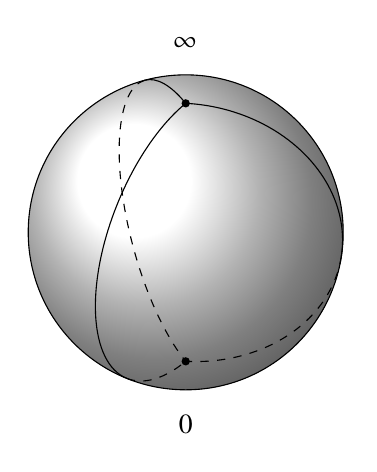
\begin{tikzpicture}[baseline=(current bounding box.center), scale=0.8]

\newcommand\pgfmathsinandcos[3]{%
  \pgfmathsetmacro#1{sin(#3)}%
  \pgfmathsetmacro#2{cos(#3)}%
}
\newcommand\LongitudePlane[3][current plane]{%
  \pgfmathsinandcos\sinEl\cosEl{#2} % elevation
  \pgfmathsinandcos\sint\cost{#3} % azimuth
  \tikzset{#1/.style={cm={\cost,\sint*\sinEl,0,\cosEl,(0,0)}}}
}
\newcommand\DrawLongitudeCircle[2][1]{
  \LongitudePlane{35}{#2} % first argument is angle of elevation
  \tikzset{current plane/.prefix style={scale=#1}}
   % angle of "visibility"
  \pgfmathsetmacro\angVis{atan(sin(#2)*cos(35)/sin(35))} % these are angle of elevation too
  % this might assume that the angle of elevation is positive
  \draw[current plane] (\angVis:1) arc (\angVis:90:1);
  \draw[current plane,dashed] (\angVis:1) arc (\angVis:-90:1);
}

% the "2.5" magic number is the radius of the sphere 
% the "35" magic number is the angle of elevation of the camera
\pgfmathsetmacro\H{2.5*cos(35)}
\filldraw[ball color=white] (0,0) circle (2.5);
\foreach \t in {-5,-125,-245} { \DrawLongitudeCircle[2.5]{\t} }
\coordinate[style={inner sep=0pt,outer sep=0pt,minimum size=3pt,
    fill=black,circle}] (O) at (0,-\H);
\node[below=16pt] at (O) {\(0\)};
\coordinate[style={inner sep=0pt,outer sep=0pt,minimum size=3pt,
    fill=black,circle}] (I) at (0,\H);
\node[above=16pt] at (I) {\(\infty\)};
\end{tikzpicture}
\end{center}
\caption{The period map at \(n = 2\), \(p = 2\)}\label{PeriodMapFigure}
\end{figure}

\begin{remark}
It is also possible to build versions of Dieudonn\'e theory over still more exotic rings.  The most successful such version is Zink's theory of \index{Dieudonn\'e module!display}Dieudonn\'e displays~\cite{ZinkDisplays}, which has found some application in algebraic topology~\cite{LawsonDisplays}.
\end{remark}









\section{Ordinary cooperations for Landweber flat theories}\label{LEFTCooperations}

\begin{center}
\textbf{Convention: We will write \(H\) for \(\HFp\) for the duration of the lecture.}
\end{center}

Our goal in this Lecture is to put Dieudonn\'e modules to work for us in algebraic topology.  The executive summary of Dieudonn\'e theory is that it gives a \emph{linear} (or \emph{logarithmic}) presentation of the theory of Hopf algebras.  From the perspective of algebraic topology, functors sending cofiber sequences to exact sequences in a linear category are precisely homology functors.  Tying these two ideas together, if we can find a functor that sends exact sequences of spaces (or spectra) to exact sequences of Hopf algebras, we can post-compose it with a suitable version of the Dieudonn\'e functor to get a homology functor and hence a \emph{spectrum}.

To meet algebraic topology in its natural setting, it will be useful to also have a version of Dieudonn\'e theory that is well-adapted to working with \emph{graded} Hopf algebras.\footnote{Another useful observation is that for a Hopf algebra arising as the ordinary homology of an infinite loopspace, its degree--zero part is always group-like.}  This falls out of an extended study of the covariant Dieudonn\'e module: it can be shown that the functor $D_*$ is representable by the \textit{$p$--typical Witt formal group} $\widehat{\mathbb W}_p$,\footnote{An extremely pleasant perspective on the construction of the Witt scheme is presented by Lazard~\cite[Chapter III]{LazardCFGs}.}\footnote{A coordinate \(x\) on \(\CP^\infty_E\) induces a sequence of isomorphisms
\begin{align*}
\CatOf{FormalGroups}(BU_E, \G) & \cong \CatOf{FormalSchemes}(\CP^\infty_E, \G) \\
& \stackrel{x}{\cong} \CatOf{FormalSchemes}(\A^1, \G) = C\G,
\end{align*}
which presents \(E^* BU\) as the Witt Hopf algebra.  However, this isomorphism is not especially interesting~\cite[Remark 18.1]{StricklandFPFP}: for one, it is \emph{highly} dependent upon the choice of coordinate, but the far right-hand object has no dependence on \(\CP^\infty_E\), and so the operations we have been studying---formal group auto- and endomorphisms of \(\CP^\infty_E\), mainly---do not act, and this isomorphism cannot be equivariant in any useful sense.} i.e.,
\begin{center}
\begin{tikzcd}
C_* \G \arrow[equal]{r} & \CatOf{FormalSchemes}(\mathbb A^1, \G) \arrow[equal]{r} & \CatOf{FormalGroups}(\widehat{\mathbb W}, \G) \\
D_* \G \arrow{u} \arrow[equal]{r} & \CatOf{FormalSchemes}(\mathbb A^1, \G)^{\ptyp} \arrow{u} \arrow[equal]{r} & \CatOf{FormalGroups}(\widehat{\mathbb W}_p, \G) \arrow{u} .
\end{tikzcd}
\end{center}
The Witt formal scheme has the additional miraculous property that it is dualizable: there is a coWitt formal scheme $\widehat{C\mathbb W}_p$ with
\begin{align*}
\CatOf{FormalGroups}(\widehat{\mathbb W}_p, \G) & \cong \CatOf{FormalGroups}(\G, \widehat{C\mathbb W}_p) \\
& \cong \CatOf{HopfAlgebras}(\sheaf O_{\widehat{C\W}_p}, \sheaf O_{\G}).
\end{align*}
We are thus moved to form graded versions of the \index{Witt vectors!Hopf algebra}coWitt Hopf algebra.  More precisely, the following theorem says that there are graded versions of the coWitt Hopf algebra that give a sequence of projective generators for the category of connected graded Hopf algebras over \(\F_p\):

\begin{theorem}[{\cite[Section 3.2]{Schoeller}, \cite[Proposition 1.6]{GLM}}]
Let \(S(n)\) denote the free graded-commutative Hopf algebra over \(\F_p\) on a single generator in degree \(n > 0\).  There is a projective cover \(H(n) \onto S(n)\), described as follows:
\begin{itemize}
\item If either of the following conditions hold...
\begin{itemize}
\item \(p = 2\) and \(n = 2^m k\) for \(2 \nmid k\) and \(m > 0\), or
\item \(p \ne 2\) and \(n = 2p^m k\) for \(p \nmid k\) and \(m > 0\),
\end{itemize}
then \(H(n) = \F_p[x_0, x_1, \ldots, x_k]\) with the Witt vector diagonal, i.e., the diagonal is arranged so that the elements \(w_j = x_0^{p^j} + p x_1^{p^{j-1}} + \cdots + x_j\) are primitive.
\item Otherwise, \(H(n) = S(n)\) is the identity.
\qed
\end{itemize}
\end{theorem}

\begin{corollary}[{\cite[Section 5]{Schoeller}}]
The category \(\CatOf{GradedHopfAlgs}^{> 0, \fin}_{\F_p/}\) of finite-type graded connected Hopf algebras under \(\F_p\) is a full subcategory of modules for the ring \[\bigoplus_{n, m} \CatOf{GradedHopfAlgs}(H(n), H(m)).\]
\end{corollary}
\begin{proof}[Construction]
This is a general nonsense consequence of having found a set of projective generators.  The functor presenting the inclusion is \[M \mapsto \bigoplus_{n=0}^\infty \CatOf{GradedHopfAlgs}(H(n), M),\] and since this functor is corepresentable its endomorphisms are encoded by the indicated ring.
\end{proof}

We would also like to give a set of conditions, analogous to the technical conditions appearing in the previous two presentations, which select this full subcategory out from all possible modules over this endomorphism ring.

\begin{definition}[{\cite[pg.\ 116]{GLM}}]
\index{Dieudonn\'e module!graded}Let \(\CatOf{GradedDMods}\) denote the category of graded abelian groups \(M\) equipped with maps\footnote{Here \(n\) is required to be even if \(p \ne 2\).}
\begin{align*}
V\co M_{pn} & \to M_n, &
F\co M_n & \to M_{pn}
\end{align*}
satisfying
\begin{enumerate}
\item \(M_{< 1} = 0\).
\item If \(n\) is odd, then \(pM_n = 0\).
\item The composites are controlled by \(FV = p\) and \(VF = p\).\footnote{These come from \(H(n) \subseteq H(pn)\) and the map \(H(pn) \to H(n)\) sending \(x_n\) to \(x_{n-1}^p\).}
\end{enumerate}
\end{definition}

\begin{remark}
Suppose that \(n\) is even, written at odd primes in the form \(n = 2p^m k\) with \(p \nmid k\) or at \(p = 2\) in the form \(n = 2^m k\) with \(2 \nmid k\) at \(p = 2\).  Then, combining the above relations, we get the torsion condition \(p^{m+1} M_n = F^{m+1} V^{m+1} M_n = 0\).
\end{remark}

\begin{theorem}[{\cite[Section 5]{Schoeller}, \cite[Theorem 1.11]{GLM}}]
The functor
\begin{align*}
D_*\co \CatOf{GradedHopfAlgs}^{>0, \fin}_{\F_p/} & \to \CatOf{GradedDMods}, \\
D_*(H) = \bigoplus_n D_n(H) & = \bigoplus_n \CatOf{GradedHopfAlgs}^{>0, \fin}_{\F_p/}(H(n), H)
\end{align*}
is an exact equivalence of categories.  Moreover, \(D_* H(n)\) is characterized by the equation
\[\pushQED{\qed}
\CatOf{GradedDMods}(D_* H(n), M) = M_n. \qedhere
\popQED\]
\end{theorem}

Having produced our desired graded Dieudonn\'e theory, we now need some topological input.  We are by now well aware that the homology of an \(H\)--space forms a Hopf algebra, and the Serre spectral sequence for a fibration of \(H\)--spaces \(F \to E \to B\) gives a spectral sequence of Hopf algebras: \[E_2^{*, *} = H^* B \otimes H^* F \Rightarrow H^* E.\]  The following result of Goerss--Lannes--Morel says that in the case that the fibration is one of \emph{infinite loopspaces}, we have the exactness property we need:

\begin{theorem}[{\cite[Lemma 2.8]{GLM}}]
Let \(X \to Y \to Z\) be a cofiber sequence of spectra.  Then, provided \(n > 1\) satisfies \(n \not\equiv \pm 1 \pmod{2p}\), there is an exact sequence
\[\pushQED{\qed}
D_n H_* \Loops^\infty X \to D_n H_* \Loops^\infty Y \to D_n H_* \Loops^\infty Z. \qedhere
\popQED\]
\end{theorem}

\noindent This Theorem is not especially easy to prove: one works very directly with unstable modules over the Steenrod algebra, the bar spectral sequence, and Postnikov decomposition of infinite loopspaces.  We refer the reader to the paper directly, as we have been unable to find a useful improvement upon or even summary of the results presented there.  Nonetheless, granting this Theorem, we use Brown representability to draw the following consequence:

\begin{corollary}[{\cite[Theorem 2.1, Remark 2.9]{GLM}}]\label{BrownGitlerSpectraDefn}
For \(n > 1\) an integer satisfying \(n \not\equiv \pm 1 \pmod{2p}\),\footnote{As convention, when \(n \equiv \pm 1 \pmod{2p}\) we set \(B(n) := B(n-1)\), and \(B(0) := \S^0\).} there exists a spectrum \(B(n)\), called the \(n\){\th} \index{Brown--Gitler spectrum}\textit{Brown--Gitler spectrum}, which satisfies \[\pushQED{\qed}B(n)_n X \cong D_n H_* \Loops^\infty X. \qedhere\popQED\]
\end{corollary}


We will now use the \(B(n)\) spectra to analyze the \index{Hopf ring}Hopf rings arising from unstable cooperations.  Our intention is to prove the following:
\begin{theorem}[{cf.\ \Cref{UnstableEthyCooperations}}]\label{LEFTUnstableCooperations}
For \(F = H\) and \(E\) a \index{Landweber flat}Landweber flat homology theory, the comparison map \[\AA(H, E) \to H_* \OS{E}{2*}\] is an isomorphism of Hopf rings.
\end{theorem}
\noindent We have previously computed that the comparison map \[\AA(H, BP) \to H_* \OS{BP}{2*}\] is an isomorphism.  In order to make use of this statement now, we must reimagine it in terms of Dieudonn\'e theory.  In order to do that, we again have to reimagine some of Dieudonn\'e theory itself, as our description of it is concerned with \emph{Hopf algebras} rather than \emph{Hopf rings}.  Recall that a Hopf ring is an algebra object \[\circ\co A_* \boxtimes A_* \to A_*,\] where ``\(\boxtimes\)'' is a kind of graded \index{Hopf algebra!tensor product}tensor product of externally graded Hopf algebras~\cite[Proposition 2.6]{HuntonTurner}, \cite[Definition 2.2]{BuchstaberLazarev}, \cite[Section 5]{GoerssDieudonne}.  Since \(D_*\) gives an equivalence of categories between internally graded Hopf algebras and internally graded Dieudonn\'e modules, we should be able to find an analogous formula for the tensor product of \index{Dieudonn\'e module!tensor product}Dieudonn\'e modules.

\begin{definition}{\cite[pg.\ 154]{GoerssDieudonne}}
Let \(M\) and \(N\) be connected graded Dieudonn\'e modules.  Their module tensor product \(M \otimes N\) receives the structure of a \(\Z_p\<V\>\)--module, where \(V(x \otimes y) = V(x) \otimes V(y)\).  We define the \textit{tensor product of Dieudonn\'e modules}\footnote{This definition is specialized to \(\F_p\) and \(\mathbb W_p(\F_p) = \Z_p\), where we don't have to worry about Frobenius semi-linearity.} by \[M \boxtimes N = \left.\frac{\Z_p\<F, V\>}{(VF = p)} \otimes_{\Z_p[V]} (M \otimes N) \middle/ \left( \begin{array}{c} 1 \otimes Fx \otimes y = F \otimes x \otimes Vy, \\ 1 \otimes x \otimes Fy = F \otimes Vx \otimes y \end{array} \right) \right. .\]
\end{definition}

\begin{lemma}[{\cite[Corollary 8.14]{GoerssDieudonne}}]
The natural map \[D_*(H) \boxtimes D_*(H') \to D_*(H \boxtimes H')\] is an isomorphism. \qed
\end{lemma}

\begin{definition}
For a ring \(R\), a \index{Dieudonn\'e module!algebra}\textit{Dieudonn\'e \(R\)--algebra} \(A_*\) is an externally graded Dieudonn\'e module equipped with an \(R\)--action and a unital multiplication \[\circ\co A_* \boxtimes A_* \to A_*.\]
\end{definition}

\begin{example}[{\cite[Proposition 10.2]{GoerssDieudonne}}]
Inspired by \Cref{UnstableRWRelation} and our interest in \(H_* \OS{E}{*}\), for a complex-oriented homology theory \(E\) we define its \textit{algebraic Dieudonn\'e \(E_*\)--algebra} by \[R_E = \left. E_*[b_1, b_2, \ldots] \middle/ \left( \begin{array}{c} b(s+t) = b(s) +_E b(t) \end{array} \right) \right.,\] where \(V\) is multiplicative, \(V\) fixes \(E_*\), and \(V\) satisfies \(Vb_{pj} = b_j\).\footnote{If \(E_*\) is torsion-free, then this determines the behavior of \(F\) by \(FV = p\).}  This is the Dieudonn\'e-theoretic analogue of the algebraic approximation \(\AA(H, E)\).  We also write \(D_E = \{D_{2m} H_* \OS{E}{2n}\}\) for the even part of the topological Dieudonn\'e algebra, and these come with natural comparison maps \[R_E \to D_E \to D_* H_* \OS{E}{2*}.\]
\end{example}

\begin{theorem}[{Dieudonn\'e theoretic form of \Cref{LEFTUnstableCooperations}, \cite[Theorem 11.7]{GoerssDieudonne}}]\label{LandweberFlatUnstableCoopns}
Restricting attention to the even parts, the maps \[R_E \to D_E \to D_* H_* \OS{E}{2*}\] are isomorphisms for \(E\) Landweber flat.
\end{theorem}
\begin{proof}
In \Cref{HopfRingForEBP}, we showed that these maps are isomorphisms for \(E = BP\).  However, the right--hand object can be identified via Brown--Gitler juggling: \[D_n H_* \OS{E}{2j} = B(n)_n \Susp^{2j} E = E_{2j+n} B(n).\]  It follows that if \(E\) is Landweber flat, then the middle-- and right--terms are determined by change-of-base from the respective \(BP\) terms.  Finally, the formation of \(R_E\) commutes with change-of-base, and the theorem follows.
\end{proof}

\begin{remark}
Goerss's original proof of \Cref{LandweberFlatUnstableCoopns}~\cite{GoerssDieudonne} involved a lot more work, essentially because he didn't want to assume \Cref{HFpBPCooperationsTheorem} or \Cref{HopfRingForEBP}.  Instead, he used the fact that \(\Susp^\infty_+ \Loops^2 S^3\) is a regrading of the ring spectrum \(\bigvee_n B(n)\), together with knowledge of \(BP_* \Loops^2 S^3\).
\end{remark}

\begin{remark}[{\cite[Proposition 11.6, Remark 11.4]{GoerssDieudonne}}]
The Dieudonn\'e algebra framework also makes it easy to add in the odd part after the fact.  Namely, suppose that \(E\) is a torsion--free ring spectrum and suppose that \(E_* B(2n)\) is even for all \(n\).  In this setting, we can verify the purely topological version of this statement: \index{homology suspension}the map \[D_E[e] / (e^2 - b_1) \to D_* H_* \OS{E}{*}\] is an isomorphism.  To see this, note that because \[E_{2n-2k-1} B(2n) \to D_{2n} H_* \OS{E}{2k+1}\] is onto and \(E_{2n-2k-1} B(2n)\) is assumed zero, the group \(D_{2n} H_* \OS{E}{2k+1}\) vanishes as well.  A bar spectral sequence argument shows that \(D_{2n+1} H_* \OS{E}{2k+2}\) is also empty~\cite[Lemma 11.5.1]{GoerssDieudonne}.  Hence, the map on even parts \[(D_E[e] / (e^2 - b_1))_{*, 2n} \to (D_* H_* \OS{E}{*})_{*, 2n}\] is an isomorphism, and we need only show that \[D_* H_* \OS{E}{2n} \xrightarrow{e \circ -} D_* H_* \OS{E}{2n+1}\] is an isomorphism as well.  Since we have \(e(Fx) = F(Ve \circ x) = 0\) generally and \(D_* A / FD_* A \cong Q^* A\) for a Hopf algebra \(A\), we see that \(e\) kills decomposables and suspends indecomposables: \[e \circ D_* H_* \OS{E}{2n} = \Susp QH_* \OS{E}{2n}.\]  This is also what happens in the bar spectral sequence, and the claim follows.  In light of \Cref{LandweberFlatUnstableCoopns}, this means that for Landweber flat \(E\), the comparison isomorphism can be augmented to a further isomorphism \[R_E[e] / (e^2 - b_1) \to D_* H_* \OS{E}{*}.\]
\end{remark}

\begin{remark}[{\cite{HopkinsHunton}}]
The results of this Lecture are accessed from a different perspective by Hopkins and Hunton, essentially by forming a tensor product of Hopf rings and showing that Landweber flatness induces a kind of flatness with respect to the Hopf ring tensor product as well.
\end{remark}


Before moving on, we prove a sequence of small results which make these spectra \(B(n)\) somewhat more tangible, though we advise the reader that these do not bear any further on our investigation of unstable cooperations.  We begin with a definition:

\begin{definition}[{\cite[Example 3.6]{GLM}}]\label{SpanierWhiteheadDualOfGeneratingModule}
Let \(G(n)\) denote the free \index{Steenrod algebra!unstable module}unstable \(\mathcal A^*\)--module on a degree \(n\) generator.\footnote{This module admits a presentation as \[G(n) = \begin{cases} \Susp^n \mathcal A / \{\beta^\eps P^i \mid 2pi + 2\eps > n\}\mathcal A & \text{if \(p > 2\)}, \\ \Susp^n \mathcal A / \{\Sq^i \mid 2i > n\}\mathcal A & \text{if \(p = 2\)}. \end{cases}\]  The Spanier--Whitehead dual of this right-module, \(DG(n)\), is given by \[\Susp^n (D G(n))^* = \begin{cases}\mathcal A / \mathcal A \{\chi(\beta^\eps P^i) \mid 2pi + 2\eps > n\} & \text{if \(p > 2\)}, \\ \mathcal A / \mathcal A \{\chi{\Sq^i} \mid 2i > n\} & \text{if \(p = 2\)}. \end{cases}\]}  For \(M\) an unstable \(\mathcal A^*\)--module, \[\CatOf{Modules}_{\mathcal A^*}(G(n), M) = M_n.\]
\end{definition}

\begin{lemma}[{\cite[Proof of Theorem 3.1, Lemma 3.2]{GLM}}]
The spectrum \(B(n)\) is connective and \(p\)--complete, and there is an isomorphism \[H_* B(n) \cong \Susp^{-n} G(n)^*.\]
\end{lemma}
\begin{proof}
First, rearrange:
\begin{align*}
\pi_k B(n) & = B(n)_n \S^{n-k} = D_n H_* \Loops^\infty \Susp^\infty S^{n-k}.
\end{align*}
If \(k < 0\), \(n\) is below the connectivity of \(\Loops^\infty \S^{n-k}\) and hence this vanishes.  The second assertion follows from the observation that \(H\Z_* B(n)\) is an \(\F_p\)--module, followed by an Adams spectral sequence argument.  To see the assertion about being an \(\F_p\)--module, restrict to the case \(n \not\equiv \pm 1 \pmod{2p}\) and calculate
\begin{align*}
H\Z_k B(n) & = B(n)_n \Susp^{n-k} H\Z \\
& = D_n H_* K(\Z, n-k) \\
& = [H(n), H_* K(\Z, n-k)]_n \\
& = [Q^* H_* K(\Z, n-k)]_n.
\end{align*}
From this, we conclude completeness.  To finish the mod--\(p\) homology calculation, note that the unstable module \(G(n)\) also enjoys a universal property in the category of \emph{stable} \(\mathcal A^*\)--modules by first passing to the maximal unstable submodule \(\Loops^\infty M\) of a stable module \(M\): \[\CatOf{Modules}_{\mathcal A^*}(G(n), M) \cong [\Loops^\infty M]_n.\]  Given this, we can perform the mod--\(p\) version of the above computation:
\begin{align*}
H_k B(n) & = D_n H_* K(\F_p, n-k) \\
& = \CatOf{Modules}_{\mathcal A^*}(G(n), \Susp^{n-k} \mathcal A_*) \\
& = \CatOf{Modules}_{\F_p}(G(n)_{n-k}, \F_p). \qedhere
\end{align*}
\end{proof}

Lastly, for a \emph{space} \(X\), we definitionally have that have \(H_* X\) forms an unstable module over the Steenrod algebra, i.e., \(\Loops^\infty H_* X = H_* X\).  This has the following direct sequence (with minor fuss at the bad indices \(n \equiv \pm 1 \pmod p\)):

\begin{corollary}[{\cite[Lemma 3.3]{GLM}}]
For \(X\) a space, there is a natural surjection \(B(n)_n X \to H_n X\). \qed
\end{corollary}

\begin{remark}[{\cite{Cohen}}]
These properties uniquely characterize the spectra \(B(n)\) as \textit{Brown--Gitler spectra}\index{Brown--Gitler spectrum}, which arise in many other settings in stable homotopy theory.  For instance, the stable James splitting for \(\Loops^2 S^3\) is given by \[\Susp^\infty_+ \Loops^2 \Susp^2 S^1 \simeq \bigvee_{j=0}^\infty \Susp^j B(\lfloor j/2 \rfloor).\]
\end{remark}










\section{Cooperations among geometric points on \texorpdfstring{\(\moduli{fg}\)}{Mfg}}\label{CoopnsForMoravaKandHA}


Our discussion of unstable cooperations has touched on each of the families of chromatic homology theories described in \Cref{DefnChromaticHomologyThys} except one: the \index{Morava K theory@Morava \(K\)--theory}\index{Morava E theory@Morava \(E\)--theory}Morava \(K\)-- and \(E\)--theories.  Our final goal before moving on to other subjects is to describe some of the \index{operations!mixed}\index{operations!unstable}mixed unstable cooperations for \((K_\Gamma)_* \OS{K_{\Gamma'}}{*}\).  In complete generality, this seems like a difficult problem: our algebraic model is rooted in formal group homomorphisms, and we have not proven any theorems about the moduli of such for arbitrary finite-height formal groups.  However, the landscape brightens considerably in the case where we pick \(\Gamma' = \G_a\), as this is the sort of calculation we considered in \Cref{LazarevComparisonOfCplxes} and \Cref{CalculationOfLTTangentSpace}.  In light of this, we specialize \(\Gamma'\) to \(\G_a\) (and hence \(K_{\Gamma'}\) to an Eilenberg--Mac Lane spectrum \(H\)), and we abbreviate \(K_\Gamma\) to just \(K\).

As with all the other major results of this Case Study, our approach will rest on the \index{bar spectral sequence}bar spectral sequence \[\Tor^{K_* \OS{H}{q}}_{*, *}(K_*, K_*) \Rightarrow K_* \OS{H}{q+1}.\]  The analysis of this spectral sequence was first accomplished by Ravenel and Wilson~\cite{RavenelWilsonKthyOfEMSpaces}, but has since been re-envisioned by Hopkins and Lurie~\cite[Section 2]{HopkinsLurie}.  In order to give an effective analysis of this spectral sequence in line with the theme of this book, we will endeavor to give algebro-geometric interpretations of its input and its output, beginning with the case \(q = 0\) and \(H = H(S^1[p^j])\) for some \(1 \le j \le \infty\).  This task begins with giving just \emph{algebraic} descriptions of the input and output.  For \(j < \infty\), we have essentially already computed the output by other means:

\begin{theorem}[{\cite[Theorem 5.7]{RavenelWilsonKthyOfEMSpaces}, \cite[Proposition 2.4.4]{HopkinsLurie}}]\label{KtheoryConvertsTorsionToTorsion}
There is an isomorphism \[BS^1[p^j]_K \cong BS^1_K[p^j].\]
\end{theorem}
\begin{proof}
The circle bundle \(S^1 \to BS^1[p^j] \to BS^1\) has associated Gysin sequence
\begin{center}
\begin{tikzcd}[row sep=0.6em]
K^* BS^1 \arrow{rr}{- \smile [p^j](x)} & & K^* BS^1 \arrow{ld} \\
& K^* BS^1[p^j] \arrow{lu}{\partial} ,
\end{tikzcd}
\end{center}
where \(x\) is any choice of coordinate on \(BS^1_{K} \cong \Gamma\).  Any \index{formal group!l series@\(\ell\)--series}\(p\)--series for \(\Gamma\) takes the form \([p](x) = c x^{p^d} + \cdots\) for \(c\) a unit.  Such an element is not a zero-divisor, so \(\partial\) vanishes, and this presents \(K^* BS^1[p^j]\) as the quotient ring \[K^* BS^1[p^j] \cong K^* BS^1 / [p^j](x). \qedhere\]
\end{proof}

\begin{remark}\label{KHomologyOfClassifyingSpace}
In the proof of the homological statement dual to \Cref{KtheoryConvertsTorsionToTorsion}, there is a corresponding exact sequence of Hopf algebras
\begin{center}
\begin{tikzcd}[row sep=0.6em]
K_* BS^1 \arrow["{- \frown [p^j](x)}", leftarrow]{rr} & & K_* BS^1 \arrow[leftarrow]{ld} \\
& K_* BS^1[p^j] \arrow["\partial", leftarrow]{lu}
\end{tikzcd}
\end{center}
where again \(\partial = 0\) and hence \(K_*(BS^1[p^j])\) is presented as the kernel of the map ``cap with \([p^j](x)\)''.  We will revisit this duality in the next Case Study.
\end{remark}

With this in hand, the analysis of the bar spectral sequence proceeds very much analogously to the example of the unstable dual Steenrod algebra of \Cref{UnstableContextsSection}.  We will analyze what \emph{must} happen in the bar spectral sequence \[\Tor^{K_* S^1[p^j]}_{*, *}(K_*, K_*) \Rightarrow K_* BS^1[p^j]\] in order to reach the conclusion of \Cref{KtheoryConvertsTorsionToTorsion}.  In the input to this spectral sequence, the ground algebra is given by a noncanonical isomorphism \[K_* \OS{H(S^1[p^j])}{0} \cong K_* \OS{H\Z/p^j}{0} = K_*[[1]] / ([1]^{p^j} - 1) = K_*[[1] - [0]] / \<[1] - [0]\>^{p^j}.\]  The \(\Tor\)--algebra for this truncated polynomial algebra \(K_*[\alpha_{()}] / \alpha_{()}^{p}\) is then given by the formula \[\Tor^{K_*[\alpha_{()}] / \alpha_{()}^{p^j}}_{*, *}(K_*, K_*) = \Lambda[\alpha'_{()}] \otimes \Gamma[\alpha_{()}],\] the combination of an exterior algebra and a divided power algebra.\footnote{In Ravenel--Wilson~\cite[Lemma 6.6]{RavenelWilsonKthyOfEMSpaces}, the elements \(\alpha_{()}\) and \(\alpha'_{()}\) are identified as a \idxentry{transpotence} and a \idxentry{homology suspension} respectively.}  We know which classes are supposed to survive this spectral sequence, and hence we know where the differentials must be~\cite[Section 8]{RavenelWilsonKthyOfEMSpaces}:
\begin{align*}
d\left(\alpha_{()}^{[p^{jd}]}\right) & = \alpha'_{()}, \\
\Rightarrow d\left(\alpha_{()}^{[i + p^{jd}]}\right) & = \alpha'_{()} \cdot \alpha_{()}^{[i]}.
\end{align*}
The spectral sequence collapses after this differential.  In the case \(1 < j < \infty\), there are some hidden multiplicative extensions in the spectral sequence, but these too are all determined by already knowing the multiplicative structure on \(K_* \OS{H(S^1[p^j])}{1}\).

However, the case of \(j = \infty\) is a bit different, beginning with the following:

\begin{lemma}
For \(q \ge 1\), \(K(\Q/\Z_{(p)}, q)\) and \(K(\Z, q+1)\) are \(p\)--adically equivalent.
\end{lemma}
\begin{proof}
This is a consequence of the fiber sequence \[K(\Q, q) \to K(\Q/\Z_{(p)}, q) \to K(\Z_{(p)}, q+1).\]  The first term has vanishing mod--\(p\) homology, forcing the \(\HFp\)--Serre spectral sequence of the fibration to collapse and for the edge homomorphism to be an isomorphism.  Similarly, the map \(K(\Z, q+1) \to K(\Z_{(p)}, q+1)\) is an equivalence on mod--\(p\) homology.
\end{proof}

\begin{remark}
Thinking of \(K(\Z, q+1)\) as \(B^q S^1\), one can also think of this theorem as giving a \(p\)--adic equivalence between \(B^q(S^1[p^\infty])\) and \(B^q S^1\)---i.e., the prime--to--\(p\) parts of \(S^1\) do not matter for \(p\)--adic homotopy theory.
\end{remark}

We use this to continue the analysis of the case \(q = 1\) and \(j = \infty\), where the Lemma gives a \(p\)--adic equivalence \(B(S^1[p^\infty]) = \CP^\infty\).  The bar spectral sequence of interest then takes the form \[\Tor^{K_* S^1}_{*, *}(K_*, K_*) \Rightarrow K_* \CP^\infty.\]  The input algebra \(K_* S^1\) is exterior on a single generator in odd degree, and so its \(\Tor\)--algebra is linearly dual to a power series algebra on a single generator in even degree.  Since all of its input is even, this spectral sequence collapses immediately.\footnote{Thinking of this as the limiting ``\(j \to \infty\)'' instance of the family of examples above is a great opportunity to meditate on the role of odd-dimensional classes in homotopy theory.}

There is a lot of structure visible in this collection of spectral sequences, as considered simultaneously.  Without further inspection, the spectral sequence at \(j = \infty\) records that \(\CP^\infty_K\) is a formal variety, and the spectral sequences at the finite values \(1 \le j < \infty\) encode in their differentials the behavior of the map \(p^j\co \Gamma \to \Gamma\) on functions.  Lastly, we notice that the \(E_\infty\) page of each finite-range spectral sequence includes into the spectral sequence at \(j = \infty\), and moreover this filtration is exhaustive: every term in the \(j = \infty\) spectral sequence appears at some \(j < \infty\) stage.  Since this last property is about the \(E_\infty\) pages, it is really a property of the formal group \(\Gamma\), which we record in a definition:

\begin{definition}[{\cite[Definition 4.1]{GrothendieckCristaux}}]\label{DefnPDivGp}
A \index{p divisible group@\(p\)--divisible group}\textit{\(p\)--divisible group}\footnote{Some like to call these \index{Barsotti--Tate group|see {\(p\)--divisible group}}\textit{Barsotti--Tate groups}, which is probably the better name, since ``\(p\)--divisible group'' does not communicate these subtle extra properties.} of height \(d\) over a field is a system \(\mathbb G_j\) of finite group schemes satisfying \(\operatorname{dim} \sheaf O(\mathbb G_j) = p^{jd}\), as well as maps \(i_k^j\co \mathbb G_k \to \mathbb G_j\) for \(k < j\) which belong to exact sequences \[0 \to \mathbb G_k \xrightarrow{i_k^j} \mathbb G_j \xrightarrow{p^k} \mathbb G_j.\]
\end{definition}

\begin{definition}
A \(p\)--divisible group is said to be \index{p divisible group@\(p\)--divisible group!connected}\textit{connected} when its constituent subgroups \(\mathbb G_j\) are infinitesimal thickenings of \(\Spec k\).  An example of this is the sequence of torsion subgroups \(\G[p^j]\) of a formal group \(\G\).  An example of a \(p\)--divisible group which is \emph{not} connected is the sequence of constant group schemes \(\mathbb G_j = S^1[p^j]\).
\end{definition}

\begin{lemma}[{\cite[Section 6.7]{GrothendieckCristaux}}]
Over a perfect field of positive characteristic \(p\), a connected \(p\)--divisible group is equivalent to a smooth formal group of finite height.
\end{lemma}
\begin{proof}[Correspondence]
The maps in both directions are easy: a \(p\)--divisible group is sent to its colimit, and a formal group of finite height is sent to its system of \(p^j\)--torsion subgroups.  In both directions there is something mild to check: that the colimit gives a formal variety, and that the system of \(p^j\)--torsion subgroups has the indicated exactness properties.
\end{proof}

\begin{remark}\label{DieudonneModsForPDivVsFormal}
Using the extension of Dieudonn\'e theory to finite group schemes described in \Cref{WorkedAlpha2Example}, the Dieudonn\'e modules of a connected \(p\)--divisible group \(\mathbb G\) and its associated formal group \(\G\) belong to a short exact sequence: \[0 \to D_*(\G) \to \Q \otimes D_*(\G) \to \colim_j D_*(\mathbb G_j) \to 0.\]
\end{remark}

We will soon see that these interrelations among the bar spectral sequences for the different Eilenberg--Mac Lane spaces, as well as the special behavior of the spectral sequence at \(j = \infty\), are generic phenomena in \(q\).  We record the steps in our upcoming induction in the following Theorem:

\begin{theorem}[{\cite[Theorems 2.4.11--13]{HopkinsLurie}}]\label{MainKThyOfEMSpacesTheorem}
The following claims give a complete description of the Morava \(K\)--theory schemes associated to the Eilenberg--Mac Lane spaces \(\OS{HS^1[p^j]}{q}\).
\begin{enumerate}
    \item The formal scheme \((\OS{H(S^1[p^\infty])}{q})_K\) is a formal variety of dimension \(\binom{d-1}{q-1}\).
    \item As a group scheme, it is a \(p\)--divisible formal group of height \(\binom{d}{q-1}\) and dimension \(\binom{d-1}{q-1}\), \((\OS{H(S^1[p])}{q-1})_K\) models its \(p\)--torsion, and the cup product induces an isomorphism \[\theta^{q-1}\co \Q / \Z_{(p)} \otimes D(\OS{H(S^1[p^\infty])}{1})^{\wedge (q-1)} \to D(\OS{H(S^1[p^\infty])}{q-1}).\]  Here \(D(G)\) denotes the \index{Dieudonn\'e module}Dieudonn\'e module associated to \(K_0(G)\), where \[K_*(G) = K_0(G) \otimes_k K_*\] is a \(p\)--divisible Hopf algebra.
    \item Consider the model \(\Q / \Z_{(p)} \cong S^1[p^\infty]\) for the \(p\)--primary part of the circle group.  For each \(j\), the short exact sequence of groups \[0 \to \frac{1/p^j \cdot \Z_{(p)}}{\Z_{(p)}} \to \frac{\Q}{\Z_{(p)}} \to \frac{\Q}{1/p^j \cdot \Z_{(p)}} \to 0\] induces a short exact sequence of group-schemes upon applying \((\OS{H(-)}{q-1})_K\).
\end{enumerate}
\end{theorem}
\begin{proof}[Proof of Part 1]\renewcommand{\qedsymbol}{\relax}
This claim turns out to be entirely algebraic and a matter of being able to compute \(H^*(\mathbb G; \G_a)\) for \(\mathbb G\) a connected \(p\)--divisible group.  This is expressed in the main algebraic result of Hopkins--Lurie:
\end{proof}

\begin{theorem}[{\cite[Theorem 2.2.10]{HopkinsLurie}}]
Let \(\mathbb G\) be a \(p\)--divisible group over a perfect field \(k\) of positive characteristic \(p\).  There is then an isomorphism \[H^*(\mathbb G; \G_a) \cong \Sym^*(\Susp H^1(\mathbb G[p], \G_a)),\] where ``\(\Susp\)'' indicates that the classes are taken to lie in degree \(2\). \qed
\end{theorem}

\begin{lemma}[{\cite[Remark 2.2.5]{HopkinsLurie}}]
If \(\mathbb G\) is a connected \(p\)--divisible group of height \(d\) and of dimension \(n\) as a formal variety, then\index{formal group!cohomology}
\[\pushQED{\qed}
\operatorname{rank}\left(H^1(\mathbb G[p]; \G_a)\right) = d - n. \qedhere
\popQED\]
\end{lemma}

\begin{remark}
In the case where \(\mathbb G = \Gamma\) is the original height \(d\) formal group of dimension \(1\), this computes \(H^*(\Gamma; \G_a)\) to be a power series algebra on \((d-1)\) generators.  This is precisely what we found by hand in \Cref{CalculationOfLTTangentSpace}.
\end{remark}

\noindent Returning to the task at hand, we assume inductively that \((\OS{H(S^1[p^\infty])}{q-1})_K\) is a connected \(p\)--divisible group of height \(\binom{d}{q-1}\) and dimension \(\binom{d-1}{q-1}\).  Since the input to the bar spectral sequence is computed by formal group cohomology (\cite{LazarevDeformations}, \cite[Example 2.3.5]{HopkinsLurie}, Proof of \Cref{Symmetric2CocycleLemma}), it follows that the instance computing \(K^* \OS{H(S^1[p^\infty])}{q}\) has as its \(E_2\)--page an even-concentrated power series algebra of dimension \[\binom{d}{q-1} - \binom{d-1}{q-1} = \binom{d-1}{q}.\]  The spectral sequence therefore collapses at this page, so that \((\OS{H(S^1[p^\infty])}{q})_K\) is a formal variety of the dimension claimed.

\begin{proof}[Proof of Part 2, with a gap]\renewcommand{\qedsymbol}{\relax}
The other claims in Part 2 are formal after we check that \(\theta^q\) is an isomorphism, since the \(p\)--power--torsion structure of \[(\OS{H(S^1[p^\infty])}{q})_K\] can be read off from its Dieudonn\'e module, as can its height.  We introduce notation to analyze this statement: set \(M\) to be the Dieudonn\'e module associated to \(K_* \CP^\infty\), i.e., \(M = D(\OS{H(S^1[p^\infty])}{1})\).  In the following diagram
\begin{center}
\begin{tikzcd}[row sep=1.2em]
0 \arrow{r} & M^{\wedge q} \arrow{r} \arrow{d}{V} & \Q \otimes M^{\wedge q} \arrow{r} \arrow{d}{V} & \Q / \Z_{(p)} \otimes M^{\wedge q} \arrow{r} \arrow{d}{V} & 0 \\
0 \arrow{r} & M^{\wedge q} \arrow{r} & \Q \otimes M^{\wedge q} \arrow{r} & \Q / \Z_{(p)} \otimes M^{\wedge q} \arrow{r} & 0
\end{tikzcd}
\end{center}
the middle map is an isomorphism.  The snake lemma then shows both that \(V\) is a surjective endomorphism of \(M^{\wedge q} \otimes \Q/\Z_{(p)}\) and that there is an isomorphism \[\ker(V\co \Q/\Z_{(p)} \otimes M^{\wedge q} \to \Q/\Z_{(p)} \otimes M^{\wedge q}) \cong \operatorname{coker}(V\co M^{\wedge q} \to M^{\wedge q}).\]  Picking any coordinate \(x\) and considering it as an element in the curves model of the Dieudonn\'e functor, we see that the right-hand side is spanned by elements \(x \sm V^{\sm I} x\), and hence the left-hand side has \(k\)--vector--space dimension \(\binom{d-1}{q}\).

By very carefully studying the bar spectral sequence, one can learn that \(\theta^q\) induces a surjection\footnote{The proof of this is quite complicated, and it rests on a pairing between the spectral sequence for \(q = 1\) and the spectral sequence at \(q - 1\), mapping to the spectral sequence for \(q\).  Remarkably, this same pairing is the main tool that powers the original approach of  Ravenel--Wilson~\cite{RavenelWilsonKthyOfEMSpaces} and of our approach to the unstable dual Steenrod algebra in \Cref{UnstableContextsSection} (cf.\ \Cref{CircProductAndDifferentials}).  There, their program is to fix \(j = 1\) and inductively analyze \(q\) using this same pairing, then use these base cases to ground a strong induction on \(j\) and \(q\), and then finally to fix \(q\) and take the limit as \(j \to \infty\).} \[\ker V|_{\Q / \Z_{(p)} \otimes M^{\wedge q}} \to \ker V|_{D(\OS{H(S^1[p^\infty])}{q})}.\]  In fact, since these two have the same rank, \(\theta^q|_{\ker V}\) is an isomorphism on these subspaces.  This is enough to conclude that \(\theta^q\) is an injection: since the action of \(V\) is locally nilpotent, if \(\theta^q\) ever failed to be an injection then we could apply \(V\) enough times to get an example of a nontrivial element in \(\ker V|_{\Q / \Z_{(p)} \otimes M^{\wedge q}}\) mapping to zero.  Finally, to show that \(\theta^q\) is surjective, we again use the local nilpotence of \(V\) to filter \(\Q / \Z_{(p)} \otimes M^{\sm q}\) by the subspaces \(\ker V^\ell\), \(\ell \ge 1\), and it is then possible (though we omit the proof) to use our understanding of \(\ker V\) to form preimages.
\end{proof}

\begin{proof}[Proof of Part 3, mostly omitted]
This proof is quite complicated, but it is, in spirit, a generalization of the observation at \(q = 1\) that the role of the odd-degree classes in the bar spectral sequence is to pair up with those classes in the image of the \([p^j]\)--map.  In fact, their main assertion is:
\begin{siderules}
\begin{quote}
We give notation for the following rings:
\begin{align*}
A & = K_0 \OS{H(S^1[p^\infty])}{q-1}, &
A' & = K_0 \OS{H(S^1[p^j])}{q-1}, &
R & = K_0 \OS{H(S^1[p^\infty])}{q}.
\end{align*}
Let \(x' \in E_2^{1, 0}\) be an element, and let \(y' \in \mathfrak m_R\) satisfy \[y' = \psi(x') \otimes v \in \Ext^2_A \otimes_k \pi_2 K \cong \mathfrak m_R / \mathfrak m_R^2.\]  Suppose that the Hopf algebra homomorphism \([p^j]\co R \to R\) carries \(y'\) to an element \(y \in \mathfrak m_R^s\), and let \(x \in E_2^{2s, 2s-2}\) denote the image of \(y\) under the composite \[\mathfrak m_R^s / \mathfrak m_R^{s+1} \cong \Ext_A^{2s} \otimes_k \pi_{2s} K \to \Ext_{A'}^{2s} \otimes_k \pi_{2s} K = E_2^{2s, 2s} \xrightarrow{-v^{-1}} E_2^{2s, 2s-2}.\]  Then \(x\) and \(x'\) survive to the \((2s - 1)\){\th} page of the bar spectral sequence, and there we have \[d_{2s-1} x' = x.\]
\end{quote}
\end{siderules}
From here, it is a matter of \emph{carefully} pairing elements (cf.\ \cite[pg.\ 60]{HopkinsLurie}).
\end{proof}

\begin{remark}
\Cref{MainKThyOfEMSpacesTheorem} admits a restatement purely in terms of \index{Hopf algebra}Hopf algebras, although Dieudonn\'e theory was essential in its proof.  The cup product gives a natural map\footnote{Note that this alternation condition becomes dramatically more complicated in the case that the formal group law and its formal group inverse series become more complicated than that of \(\G_a\).}\index{Hopf algebra!alternating} \[K_* \OS{H(S^1[p^j])}{1}^{\wedge q} \to K_* \OS{H(S^1[p^j])}{q}.\]  The main result of this section is that this map is an isomorphism for all \(q\), and indeed that the map from the free exterior \emph{Hopf ring} maps isomorphically to the topological Hopf ring.
\end{remark}

\begin{remark}[{\cite[Section 3]{HopkinsLurie}, \cite{HedayatzadehFieldCase}, \cite{HedayatzadehGeneralCase}}]\label{EThyOfEMSpaces}
Because \(K^* \OS{H\Z/p^j}{q}\) is even, you can hope to augment this to a calculation of \(E^* \OS{H\Z/p^j}{q}\) for \(E = E_\Gamma\) the associated continuous Morava \(E\)--theory.  This is indeed possible, and the analogous formula is true at the level of Hopf algebras: \[E_* \OS{H(S^1[p^j])}{q} \cong E_* \OS{H(S^1[p^j])}{1}^{\wedge q}.\] However, the attendant algebraic geometry is quite complicated: you either need a form of Dieudonn\'e theory that functions over \(\context{E_\Gamma}\) (and then attempt to drag the proof above through that setting), or you need to directly confront what ``\index{p divisible group@\(p\)--divisible group!alternating power}alternating power of a \(p\)--divisible group'' means at the level of \(p\)--divisible groups (and forego all of the time-saving help afforded to you by Dieudonn\'e theory).
\end{remark}

\begin{remark}[{cf.\ \Cref{StableMixedKthyCoopnsVanish}}]
Notice that if we let the \(q\)--index tend to \(\infty\) in \(K_* \OS{H}{q+1}\), we get the \(K\)--homology of a point.  This is another way to see that the stable cooperations \(K_* H\) vanish, meaning that the \emph{only} information present comes from unstable cooperations.
\end{remark}

\begin{remark}
Although the method of starting with the \(j = \infty\) case and deducing from it the \(1 \le j < \infty\) cases is due to Hopkins and Lurie, the observation that the spectral sequence at \(j = \infty\) is remarkably simple had already been made by Ravenel and Wilson~\cite[Theorem 12.3]{RavenelWilsonKthyOfEMSpaces},~\cite[Theorem 8.1.3]{RWY}.
\end{remark}

\begin{remark}
\Cref{MainKThyOfEMSpacesTheorem} has a statement in the language of \Cref{UnstableAlgebraicModelSection}.  Abbreviating \(H = H(S^1[p^j])\), rather than forming the algebraic approximation
\begin{align*}
\AA(K, H) & = K_*(\CP^\infty)_{K_*[H^*]}^{\circulatearrows}[H^* \CP^\infty]
\intertext{as usual, we form the modified version}
\AA_{p^j}(K, H) & = K_*(\OS{H}{1})_{K_*[H^*]}^{\circulatearrows}[H^* \OS{H}{1}].
\end{align*}
Using the same unstable Kronecker pairing, this supports a natural map to \(K_* \OS{H}{*}\), and a summary of this Lecture's results is that it is an isomorphism.  This auxiliary approximation has two interesting features: it makes use of \emph{odd}--dimensional Eilenberg--Mac Lane spaces, and it is an elaborate name for the alternating Hopf ring on the Hopf algebra \(K_* \OS{H}{1}\).
\end{remark}













% -*- root: main.tex -*-

\chapter{The \texorpdfstring{$\sigma$}{sigma}-orientation}\label{ChapterSigmaOrientation}

By this point, we have seen a great many ways that algebraic geometry exerts control over the behavior of homotopy theory, stable and unstable.  The goal in this Case Study is to explore a setting where algebraic geometry is itself tightly controlled: whereas the behavior of formal groups is quite open-ended, the behavior of \emph{abelian varieties} is comparatively strict.  We import this strictness into algebraic topology by stiudying complex-orientable cohomology theories $E$ which have been tagged with an auxiliary abelian variety $A$ via an isomorphism $\phi\co \CP^\infty_E \cong A^\wedge_0$.  In the case that $A$ is an elliptic curve, this is our definition of an \textit{elliptic cohomology theory}.  The idea, then, is not that this puts serious constraints on the formal group $\CP^\infty_E$ (although it does place some), but rather that the theory of abelian varieties endows $A$, and hence $A^\wedge_0$, with various bits of preferred data.  This is the tack we take to construct a \emph{canonical} $MU[6, \infty)$--orientation of $E$: for any complex-orientable $E$, we identify the collection of such ring maps with ``$\Theta$--structures on $\CP^\infty_E$''; a basic theorem about abelian varieties endows the elliptic curve $A$ with a canonical such structure; and altogether this yields the desired orientation for an elliptic spectrum.

Making the identification of $MU[6, \infty)$--orientations with $\Theta$--structures requires real work, but many of the stepping stones are now in place.  We begin with a technical section about especially nice formal schemes, called \textit{coalgebraic}, and we use this to finally give the proof, announced back in \Cref{DivConstructionsAreFree}, that the scheme of stable Weil divisors on a formal curve presents the free formal group on that curve.  With that out of the way and with $MU[6, \infty)$ in mind as the eventual goal, we then summarize the behavior of the part of the Postnikov tower for complex bordism that we \emph{do} understand---the cases of $MUP$ and $MU$---and use this to make an analysis of $MSU$.  In particular, we rely heavily on the results from \Cref{ComplexBordismChapter} and \Cref{ChapterFiniteSpectra} to understand the co/homological behaviors of $BU \times \Z$, $BU$, $MUP$, and $MU$.

The coherence of all of these statements gives us very explicit target theorems to aim for in our study of $MU[6, \infty)$, but we are forced to approach them from a different vantage point: whereas we can prove a splitting principle for $SU$--bundles, the analogous statement for $U[5, \infty)$--bundles does not appear to admit a direct proof.  Consequently, the proofs of the other structure theorems for $BU[6, \infty)$ and $MU[6, \infty)$ are made considerably more complicated because we have to work with our splitting principle hands tied.  Instead, our main tools are the results developed in \Cref{UnstableCooperationsChapter}, which give us direct access to the co/homology of the layers of the Postnikov tower.  When the dust of all this settles, we will have arrived at a very satisfying and complete theory of $MU[6, \infty)$--orientations, applicable to an arbitrary complex-orientable cohomology theory.

The reader gifted with an exceptional attention span will recall from the Introduction that we were \emph{really} interested in $M\String$--orientations, and that our interest in $MU[6, \infty)$--orientations was itself only a stepping stone.  We close this Case Study with an analysis of this last setting, where we finally yield and place more hypotheses on $E$---a necessity for gaining calculational access to co/homological behavior of objects like $B\String$, which lie outside of the broader complex-orientable story.

We also give a short r\'esum\'e on the theory of elliptic curves in \Cref{SectionEllipticCurvesAndThetaFunctions}, extracting the smallest possible subset of their theory that we will need here.









\section{Coalgebraic formal schemes}

We will now finally address an elephant that has been lingering in our metaphorical room: in the first third of this book we were primarily interested in the formal scheme associated to the \emph{cohomology} of a space, but in the second third we were primarily interested in a construction converting the \emph{homology} of a spectrum to a sheaf over a context.  Our goal for today is to, when possible, put these two variances on even footing.  Our motivation for putting this lingering discrepancy to rest is more technical than aesthetic: we have previously wanted access to certain colimits of formal schemes (e.g., in \Cref{DivConstructionsAreFree}).  While such colimits are generally forbidding, similarly to colimits of manifolds, we will in effect produce certain conditions under which they are accessible.

For $E$ a ring spectrum and $X$ a space, the diagonal map $\Delta\co X \to X \times X$ induces a multiplication map on $E$--cohomology via the composite \[E^* X \otimes_{E^*} E^* X \xrightarrow{\text{K\"unneth}} E^*(X \times X) \xrightarrow{E^* \Delta} E^* X.\]  Dually, applying $E$--homology, we have a pair of maps \[E_* X \xrightarrow{E_* \Delta} E_*(X \times X) \xleftarrow{\text{K\"unneth}} E_* X \otimes_{E_*} E_* X,\] where, remarkably, the K\"unneth map goes the wrong way to form a composite.  In the case that that map is an isomorphism, the long composite induces the structure of an $E_*$--coalgebra on $E_* X$.  In the most generous case that $E$ is a field spectrum (in the sense of \Cref{FieldSpectraAreKTheories}), the K\"unneth map is always invertible and, moreover, $E^* X$ is functorially the linear dual of $E_* X$.  This motivates us to consider the following purely algebraic construction:

\begin{definition}
Let $C$ be a coalgebra over a field $k$.  We define a functor
\begin{align*}
\Sch C\co \CatOf{Algebras}_{k/} & \to \CatOf{Sets}, \\
T & \mapsto \left\{f \in C \otimes T \middle| \begin{array}{c} \Delta f = f \otimes f \in (C \otimes T) \otimes_T (C \otimes T), \\ \eps f = 1 \end{array} \right\}.
\end{align*}
\end{definition}

\begin{lemma}
For a field $k$ and a $k$--algebra $A$ which is finite--dimensional as a $k$--module, there is a natural isomorphism $\Spec A \cong \Sch A^*$.
\end{lemma}
\begin{proof}[Proof sketch]
A point $f \in (\Sch A^*)(T) \subseteq A^* \otimes T$ gives rise to a $k$--module map $f_*\co A \to T$, which the extra conditions in the formation of $(\Sch C)(T)$ force to be a ring homomorphism.  The finiteness assumption is present exactly so that $A$ is its own double--dual, giving an inverse assignment.
\end{proof}

If we drop the finiteness assumption, then this comparison proof fails entirely.  Indeed, the multiplication on $A$ gives rise only to maps \[A^* \to (A \otimes_k A)^* \from A^* \otimes_k A^*,\] which is not enough to make $A^*$ into a $k$--coalgebra.  However, if we start instead with a $k$--coalgebra $C$ of infinite dimension, the following result is very telling:

\begin{lemma}[{\cite[pg.\ 12]{Demazure}, \cite[Appendix 5.3]{Michaelis}, \cite[Remark 1.1.8]{HopkinsLurie}}]\label{kCoalgebrasAreIndFinite}
For $C$ a coalgebra over a field $k$, any finite--dimensional $k$--linear subspace of $C$ can be finitely enlarged to a subcoalgebra of $C$.  Accordingly, taking the colimit gives a canonical equivalence
\[\pushQED{\qed}
\Ind(\CatOf{Coalgebras}_k^{\mathrm{fin}}) \xrightarrow{\simeq} \CatOf{Coalgebras}_k. \qedhere
\popQED\]
\end{lemma}

\noindent This result allows us to leverage our duality Lemma pointwise: for an arbitrary $k$--coalgebra, we break it up into a lattice of finite $k$--coalgebras, and take their linear duals to get a reversed lattice of finite $k$--algebras.  Altogether, this indicates that $k$--coalgebras generally want to model \emph{formal schemes}.

\begin{corollary}\label{CoalgsAndFSchsAgreeOverk}
For $C$ a coalgebra over a field $k$ expressed as a colimit $C = \colim_k C_k$ of finite subcoalgebras, there is an equivalence \[\Sch C \cong \{\Spec C_k^*\}_k.\]  This induces a \emph{covariant} equivalence of categories \[\CatOf{Coalgebras}_k \cong \CatOf{FormalSchemes}_{/k}.\]  This equivalence translates between the product of formal schemes, the tensor product of pro-algebras, and the tensor product of coalgebras. \qed
\end{corollary}

This covariant algebraic model for formal schemes is very useful.  For instance, this equivalence makes the following calculation trivial:
\begin{lemma}[{cf.\ \Cref{HF2BOIsSymAlg}, \Cref{DivConstructionsAreFree}, and \Cref{ECohomBUIsFree}}]
Select a coalgebra $C$ over a field $k$ together with a pointing $k \to C$.  Write $M$ for the coideal $M = C / k$.  The free formal monoid on the pointed formal scheme $\Sch k \to \Sch C$ is given by \[F(\Sch k \to \Sch C) = \Sch \Sym^* M.\]  Writing $\Delta c = \sum_j \ell_j \otimes r_j$ for the diagonal on $C$, the diagonal on $\Sym^* C$ is given by
\[\pushQED{\qed}
\Delta(c_1 \cdots c_n) = \sum_{j_1, \ldots, j_n} (\ell_{1,j_1} \cdots \ell_{n, j_n}) \otimes (r_{1, j_1} \cdots r_{n, j_n}). \qedhere
\popQED\]
\end{lemma}

It is unfortunate, then, that when working over a ring rather than a field \Cref{kCoalgebrasAreIndFinite} fails~\cite[Appendix 5.3]{Michaelis}.  Nonetheless, it is possible to bake into the definitions the machinery needed to get a good-enough analogue of \Cref{CoalgsAndFSchsAgreeOverk}.

\begin{definition}[{\cite[Definition 4.58]{StricklandFSFG}}]\label{DefnCoalgebraicFormalScheme}
Let $C$ be an $R$--coalgebra which is free as an $R$--module.  A basis $\{x_j\}$ of $C$ is said to be a \index{good basis}\textit{good basis} when any finite subcollection of $\{x_j\}$ can be finitely enlarged to a subcollection that spans a subcoalgebra.  The coalgebra $C$ is itself said to be \textit{good} when it admits a good basis.  A formal scheme $X$ is said to be \index{scheme!coalgebraic}\textit{coalgebraic} when it is isomorphic to $\Sch C$ for a good coalgebra $C$.
\end{definition}

\begin{example}\label{FVarsAreCoalgebraic}
The formal scheme $\A^n$ is coalgebraic.  Beginning with the presentation \[\A^n = \Spf R\ps{x_1, \ldots, x_n} = \colim_J \Spec R[x_1, \ldots, x_n] / (x_1^{j_1}, \ldots, x_n^{j_n}),\] write $A_J$ for the algebra on the right-hand side.  Each $A_J$ is a free $R$--module, and we write \[C_J = A_J^* = R\{\beta_K \mid K < J\}\] for the dual coalgebra, with \[\beta_K(x^L) = \begin{cases} 1 & \text{if $K = L$}, \\ 0 & \text{otherwise}. \end{cases}\]  The elements $\beta_K$ form a good basis for the full coalgebra $C = \colim_J C_J$: any finite collection of them $\{\beta_K\}_{K \in \mathcal K}$ is contained inside any $C_J$ satisfying $K < J$ for all $K \in \mathcal K$.  As an additional consequence, all formal varieties are coalgebraic.
\end{example}

The main utility of this condition is that it gives us access to colimits of formal schemes:

\begin{theorem}[{\cite[Proposition 4.64]{StricklandFSFG}}]\label{CoalgebraicColimitsExist}
Suppose that $F\co \CatOf I \to \CatOf{Coalgebras}_R$ is a colimit diagram of coalgebras such that each object in the diagram, including the colimit point, is a good coalgebra.  Then \[\Sch \circ \, F\co \CatOf I \to \CatOf{FormalSchemes}\] is a colimit diagram of formal schemes. \qed
\end{theorem}

\noindent For an example of the sort of constructions that become available via this Theorem, we prove the following Corollary by analyzing the symmetric power of coalgebras:

\begin{corollary}[{\cite[Example 4.65 and Proposition 6.4]{StricklandFSFG}}]\label{ProofOfFreeFormalMonoids}
When a formal scheme $X$ is coalgebraic, the symmetric power $X^{\times n}_{\Sigma_n}$ exists.  In fact, $\coprod_{n \ge 0} X^{\times n}_{\Sigma n}$ models the free formal monoid on $X$.  Given an additional pointing $\Spec R \to X$, the colimit of the induced system \[\colim \left(\cdots \to X^{\times n}_{\Sigma_n} = \Spec R \times X^{\times n}_{\Sigma_n} \to X \times X^{\times n}_{\Sigma_n} \to X^{\times(n+1)}_{\Sigma_{n+1}} \to \cdots\right)\] models the free formal monoid on the pointed formal scheme.
\end{corollary}
\begin{proof}[Proof sketch]
The main points entirely mirror the case over a field: the symmetric power construction gives models for $X^{\times n}_{\Sigma_n}$, the symmetric algebra construction gives a model for the free formal monoid, and the stabilization against the pointing is modeled by inverting an element in the symmetric algebra.  In each case, choosing a good basis for the coalgebra underlying $X$ yields choices of good bases for the coalgebras arising from these constructions, essentially because their elements are crafted out of finite combinations of the elements of the original.
\end{proof}

In the specific case that $\Spec R \to X$ is a pointed formal \emph{curve}, we can prove something more:
\begin{corollary}[{\cite[Proposition 6.12]{StricklandFSFG}}]\label{FreeFormalGroupOnACurve}
For $\Spec R \to X$ a pointed formal curve, the free formal monoid is automatically an abelian group.
\end{corollary}
\begin{proof}[Proof sketch]
The main idea is that the coalgebra associated to a formal curve admits an increasing filtration $F_k$ so that the reduced diagonal $\overline \Delta = \Delta - (1 \otimes \eta) - (\eta \otimes 1)$ reduces filtration degree: \[\overline \Delta|_{F_k}\co F_k \to \sum_{\substack{i,j > 0 \\ i+j=k}} F_i \otimes F_j.\]  In turn, the symmetric algebra on the coalgebra associated to a formal curve inherits enough of this filtration that one can iteratively solve for a Hopf algebra antipode.
\end{proof}

We now reconnect this algebraic discussion with the algebraic topology that spurred it.

\begin{lemma}
If $E$ and $X$ are such that $E_* X$ is an $E_*$--coalgebra and \[E^* X = \CatOf{Modules}_{E_*}(E_* X, E_*),\] then there is an equivalence \[\Sch E_* X \cong X_E.\]
\end{lemma}
\begin{proof}
We have defined $X_E$ to have formal topology induced by the compactly generated topology of $X$, and this same topology can also be used to write $\Sch E_* X$ as the colimit of finite $E_*$--coalgebras.
\end{proof}

\begin{example}[{cf.\ \Cref{KtheoryConvertsTorsionToTorsion} and \Cref{KHomologyOfClassifyingSpace}}]
For a Morava $K$--theory $K_\Gamma$ associated to a formal group $\Gamma$ of finite height, we have seen that there is an exact sequence of Hopf algebras \[K_\Gamma^0(BS^1) \xrightarrow{[p^j]} K_\Gamma^0(BS^1) \to K_\Gamma^0(BS^1[p^j]),\] presenting $(BS^1[p^j])_K$ as the $p^j$--torsion formal subscheme $BS^1_K[p^j]$.  The Hopf algebra calculation also holds in $K$--homology, where there is instead the exact sequence \[(K_\Gamma)_0 B(S^1[p^j]) \to (K_\Gamma)_0 BS^1 \xrightarrow{(-)^{\ast p^j}} (K_\Gamma)_0 BS^1\] presenting $(K_\Gamma)_0 B(S^1[p^j])$ as the $p^j$--order $\ast$--nilpotence in the middle Hopf algebra.  Applying $\Sch$ to this last line covariantly converts this second statement about Hopf algebras to the corresponding statement above about the associated formal schemes---i.e., the behavior of the homology Hopf algebra is a direct reflection of the behavior of the formal schemes.
\end{example}

The example above, where the space in question is an $H$--space, also spurs us to consider a certain ``wrong-way'' operation.  We have seen that the algebra structure of the $K$--cohomology of a space and the coalgebra structure of the $K$--homology of the same space contain equivalent data: they both give rise to the same formal scheme.  However, in the case of a commutative $H$--space, the $K$--homology and $K$--cohomology give \emph{commutative and cocommutative Hopf algebras}.  Hence, in addition to considering the coalgebraic formal scheme $\Sch (K_\Gamma)_0 B(S^1[p^j])$, we can also consider the affine scheme $\Spec (K_\Gamma)_0 B(S^1[p^j])$.  This, too, should contain identical information, and this is the subject of Cartier duality.

\begin{definition}[{\cite[Sections 6.3--4]{StricklandFSFG}}]\label{DefnCartierDual}
The \index{Cartier dual}\textit{Cartier dual} of a commutative finite group scheme $G$ is defined by the formula \[DG = \InternalHom{GroupSchemes}(G, \Gm),\] itself a finite group scheme.  More generally, the Cartier dual of a commutative \emph{coalgebraic} formal group $\G$ can also be defined by \[D\G = \InternalHom{GroupSchemes}(\G, \Gm).\]
\end{definition}

\begin{lemma}[{\cite[Proposition 6.19]{StricklandFSFG}}]
Let $\G$ be a coalgebraic commutative formal group over a formal scheme $X$, and write $\mathbb H = \Spec \sheaf O_{\G}^*$ for the group scheme associated to its dual Hopf algebra.  Cartier duality then has the effects $D\G = \mathbb H$ and $D\mathbb H = \G$.
\end{lemma}
\begin{proof}
We show that the first two objects, $D\G$ and $\mathbb H$, represent the same object.  A point $(u, f) \in D\G(T)$ is specified by a pair of functions \[\left(u\co \Spec T \to X, f\co u^* \G \to u^*(\Gm \times X)\right).\]  The map $f$ is equivalent to a map of Hopf algebras $f^*\co T[u^\pm] \to \sheaf O_{\G} \otimes_{\sheaf O_X} T$, which is determined by its value $f^*(u) \in \sheaf O_{\G} \otimes_{\sheaf O_X} T$, which must satisfy the two relations $\Delta(f^* u) = f^* u \otimes f^* u$ and $\eps(f^* u) = 1$.  Invoking linear duality, $f^* u$ can also be considered as an element of $\CatOf{Modules}_{\sheaf O_X}(\sheaf O_{\G}^*, T)$, and the two relations on $f^* u$ show that it lands in the subset \[f^* u \in \CatOf{Algebras}_{\sheaf O_X /}(\sheaf O_{\G}^*, T) \subseteq \CatOf{Modules}_{\sheaf O_X}(\sheaf O_{\G}^*, T).\]  This assignment is invertible, and the proof is entirely similar for $D \mathbb H \cong \G$.
\end{proof}

\begin{remark}[{\cite[pg.\ 72]{Demazure}}]
The effect of Cartier duality on the Dieudonn\'e module of a formal group is \emph{also} described by linear duality.  Hence, the covariant and contravariant Dieudonn\'e modules described in \Cref{SectionDieudonneModules} can be taken to be related by Cartier duality.
\end{remark}

\begin{remark}\label{TopologicalCartierDuality}
Cartier duality intertwines the homological and cohomological schemes assigned to a commutative $H$--space.  When such a commutative $H$--space $X$ has free and even $E$--homology, there is an isomorphism \[D(\Spf E^0 X) = DX_E = \InternalHom{GroupSchemes}(X_E, \Gm) \cong \Spec E_0 X.\]
\end{remark}












\section{Special divisors and the special splitting principle}\label{MSUDay}

Starting today, after our extended interludes on chromatic homotopy theory and cooperations, we are going to return to thinking about bordism orientations directly.  To begin, we will summarize the various perspectives already adopted in \Cref{ComplexBordismChapter} when we were studying complex orientations of ring spectra.
\begin{enumerate}
\item (\Cref{DefnComplexOrientation}:) A complex--orientation of $E$ is, definitionally, a map $MUP \to E$ of ring spectra in the homotopy category.
\item (\Cref{ComplexOrientationsInTermsOfTrivs}:) A complex--orientation of $E$ is also equivalent to a multiplicative system of Thom isomorphisms for complex vector bundles.  Such a system is determined by its value on the universal line bundle $\L$ over $\CP^\infty$.  We can also phrase this algebro-geometrically: such a Thom isomorphism is the data of a trivialization of the Thom sheaf $\ThomSheaf{\L}$ over $\CP^\infty_E$.
\item (\Cref{OrientationsOnEAndMU}:) Ring spectrum maps $MUP \to E$ induce on $E$--homology maps $E_0 MUP \to E_0$ of $E_0$--algebras.  This, too, can be phrased algebro-geometrically: these are elements of $(\Spec E_0 MUP)(E_0)$.
\end{enumerate}
We can summarize our main result about these perspectives as follows:
\begin{theorem}[{\cite[Example 2.53]{AHSTheoremOfTheCube}}]\label{BUZTriumvirate}
Take $E$ to be \emph{complex--orientable}.  The functor
\begin{align*}
\CatOf{AffineSchemes}_{/\Spec E_0} & \to \CatOf{Sets}, \\
(\Spec T \xrightarrow{u} \Spec E_0) & \mapsto \left\{ \text{trivializations of $u^* \ThomSheaf{\L}$ over $u^* \CP^\infty_E$} \right\}
\end{align*}
is isomorphic to the affine scheme $\Spec E_0 MUP$.  Moreover, the $E_0$--points of this scheme biject with ring spectrum maps $MUP \to E$.
\end{theorem}
\begin{proof}[Proof summary]
The equivalence between (1) and (3)---i.e., between complex-orientations and $E_0$--points of $\Spec E_0 MUP$---follows from calculating that $E_0 MUP$ is a free $E_0$--module, so that there is a collapse in the universal coefficient theorem.  Then, the equivalence between (1) and (2) follows from the splitting principle for complex line bundles, which says that the first Chern class of $\L$---i.e., a trivialization of $\ThomSheaf{\L}$---determines the rest of the map $MUP \to E$.
\end{proof}

An analogous result holds for ring spectrum maps $MU \to E$ and the line bundle $1 - \L$, and it is proven in analogous way.  In particular, we will want a version of the splitting principle for virtual vector bundles of virtual rank $0$.  Given a finite complex $X$ and such a rank $0$ virtual vector bundle, write $\tilde V \co X \to BU$ for the classifying map.  Because $X$ is a finite complex, there exists an integer $n$ so that $\tilde V = -(n \cdot 1 - V)$ for an honest rank $n$ vector bundle $V$ over $X$.  Using \Cref{OriginalSplittingPrinciple}, the splitting $f^* V \cong \bigoplus_{i=1}^n \L_i$ over $Y$ gives a presentation of $\tilde V$ as \[\tilde V = -(n \cdot 1 - V) = -\bigoplus_{i=1}^n (1 - \L_i).\]  Crucially, we have organized this sum \emph{entirely in terms of bundles classified by $BU$}, as each bundle $1 - \L_i$ itself has the natural structure of a rank $0$ virtual vector bundle.  This version of the splitting principle, together with our extended discussion of formal geometry, begets the following analogue of the previous result:
\begin{theorem}[{\cite[Example 2.54]{AHSTheoremOfTheCube}, cf.\ also \cite[Lemma 6.2]{AndoStrickland}}]\label{BUTriumvirate}
Take $E$ to be complex--orientable.  The functor
\begin{align*}
\CatOf{AffineSchemes}_{/\Spec E_0} & \to \CatOf{Sets}, \\
(\Spec T \xrightarrow{u} \Spec E_0) & \mapsto \left\{ \text{trivializations of $u^* \ThomSheaf{1 - \L}$ over $u^* \CP^\infty_E$} \right\}
\end{align*}
is isomorphic to the affine scheme $\Spec E_0 MU$.  Moreover, the $E_0$--points of this scheme biject with ring spectrum maps $MU \to E$. \qed
\end{theorem}

In \Cref{ProjectivizationLecture}, we preferred to think of the cohomology of a Thom spectrum as a sheaf over the formal scheme associated to its base space.  This extra structure has not evaporated in the homological context---it just takes a different form.
\begin{lemma}
For $\xi\co G \to BGL_1 \S$ a group map, the Thom spectrum $T\xi$ is a $(\Susp^\infty_+ G)$--cotorsor.
\end{lemma}
\begin{proof}[Construction]
The Thom isomorphism $T\xi \sm T\xi \simeq T\xi \sm \Susp^\infty_+ G$ composes with the unit map $\S \to T\xi$ to give the \index{Thom diagonal}\textit{Thom diagonal} \[T\xi \to T\xi \sm \Susp^\infty_+ G. \qedhere\]
\end{proof}

\noindent Applying $\Spec E_0(-)$, the Thom diagonal is translated into the structure of a free and transitive action map \[\Spec E_0 T(\xi) \times \Spec E_0 G \to \Spec E_0 T(\xi).\]  This construction is natural in the formation of $G$ or $\xi$, and so we are also moved to specialize to the cases of $G = \Z \times BU$ and $G = BU$ and to understand $\Spec E_0 G$ in those contexts.  Again, this is a matter of chaining together results we have already proven:
\begin{align*}
\Spec E_0(\Z \times BU) & = D((\Z \times BU)_E) \tag{\Cref{TopologicalCartierDuality}} \\
& = D(\Div \CP^\infty_E) \tag{\Cref{ECohomBUIsFree}} \\
& = \InternalHom{FormalGroups}(\Div \CP^\infty_E, \Gm) \tag{\Cref{DefnCartierDual}} \\
& = \InternalHom{FormalSchemes}(\CP^\infty_E, \Gm), \tag{\Cref{ProofOfFreeFormalMonoids}} \\
\intertext{and similarly}
\Spec E_0(BU) & = \InternalHom{FormalSchemes}_{*/}(\CP^\infty_E, \Gm)
\end{align*}
is the subscheme of those maps sending the identity point of $\CP^\infty_E$ to the identity point of $\Gm$.  Such functions can be identified with trivializations of the trivial sheaf over $\CP^\infty_E$, and the action map induced by the Thom diagonal belongs to a commuting square
\begin{center}
\begin{tikzcd}
\begin{array}{c}\Spec E_0 MU \\ \times \\ \Spec E_0 BU\end{array} \arrow{r} \arrow[equal]{d} & \Spec E_0 MU \arrow[equal]{d} \\
\begin{array}{c} \{\text{triv\textsuperscript{ns} of $\ThomSheaf{1 - \L} \downarrow \CP^\infty_E$}\} \\ \times \\ \{\text{triv\textsuperscript{ns} of $1 \downarrow \CP^\infty_E$}\} \end{array} \arrow{r} & \{\text{triv\textsuperscript{ns} of $\ThomSheaf{1 - \L} \otimes 1 \downarrow \CP^\infty_E$}\}.
\end{tikzcd}
\end{center}

\begin{remark}[{\cite[Corollary 2.30 and Theorem 2.50]{AHSTheoremOfTheCube}}]\label{BUtoBUZ}
The topological maps
\begin{align*}
BU & \to \Z \times BU, &
MU & \to MUP
\end{align*}
induce recognizable algebro-geometric maps upon application of $\Spec E_0(-)$.  The comparison map \[(\Spec E_0(\Z \times BU))(T) \to \InternalHom{FormalSchemes}(\CP^\infty_E, \Gm)\] reads off the image of a map $f\co E_0(\Z \times BU) \cong E_0[b_0^\pm, b_1, \ldots] \to T$ as the components of a function $\sum_j f(b_0^j b_j) x^j \in T \otimes \sheaf O_{\CP^\infty_E}$, whereas the comparison map for $BU$ reads off the image of a map $g\co E_0(BU) \cong E_0[b_0^\pm, b_1, b_2, \ldots] / (b_0 = 1) \to T$ as the components of a function $\sum_j g(b_j)x^j$, effecting a normalizing division by $b_0$, itself the image of $\CP^0_E \subseteq \CP^\infty_E$ in $\Gm$.  Geometrically, this gives the commuting square
\begin{center}
\begin{tikzcd}
\Spec E_0(\Z \times BU) \arrow{r} \arrow[equal]{d} & \Spec E_0(BU) \arrow[equal]{d} \\
\InternalHom{FormalSchemes}(\CP^\infty_E, \Gm) \arrow{r} & \InternalHom{FormalSchemes}_{*/}(\CP^\infty_E, \Gm) \\
f(t) \arrow[|->]{r} & f(t) / f(0).
\end{tikzcd}
\end{center}

At the level of Thom spectra, these identifications are controlled by the Chern classes associated to these bundles, and the briefest way to summarize their relationship is this.  The spaces $\Z \times BU$ and $BU$ are the $0${\th} and $2${\nd} spaces in the $\Omega$--spectrum for connective complex $K$--theory, and since connective complex $K$--theory is complex-orientable, we have $kU^*(\CP^\infty) = \Z[\beta]\ps{c_1}$.  Inside this ring there is the relation \[\beta c_1 = (1 - \L).\]  Recognizing $\beta$ as the restriction of the tautological bundle on $\CP^\infty$ to $S^2 \simeq \CP^1$ and employing \Cref{Pi2AndInvariantDiffls}, this says that the trivialization $f$ of $\ThomSheaf{u^* \L}$, corresponding to a point in $(\Spec E_0 MUP)(T)$ and to $(1 - \L) \in kU^0(\CP^\infty) = [\CP^\infty, \Z \times BU]$, is sent to the trivialization $f'(0) / f$ of $\ThomSheaf{u^*(1 - \L)}$, corresponding to the induced point in $(\Spec E_0 MU)(T)$ and to $c_1 \in kU^2(\CP^\infty) = [\CP^\infty, BU]$.
\end{remark}


This last remark indicates a direction of possible generalization to the other spaces in the $\Omega$--spectrum for connective complex $K$--theory, which have the following polite description:
\begin{lemma}
There is an equivalence \[\OS{kU}{2k} = BU[2k, \infty).\]
\end{lemma}
\begin{proof}
Consider the element $\beta^k \in kU_* = \Z[\beta]$.  The source of the induced map $\beta^k\co \Susp^{2k} kU \to kU$ is $2k$--connective, and hence there is a factorization \[\Susp^{2k} kU \to kU[2k, \infty) \to kU.\]  Then, the structure of the homotopy ring $kU_*$ shows that this is an equivalence: every class of degree at least $2k$ can be uniquely written as a $\beta^k$--multiple.\footnote{Similarly, there is an equivalence $\OS{kO}{8k} = BO[8k, \infty)$, and this \emph{does not hold} for indices which are not precise multiples of $8$.}  Applying $\Loops^\infty$ gives the desired statement: \[\OS{kU}{2k} = \Loops^\infty \Susp^{2k} kU \simeq \Loops^\infty kU[2k, \infty) = BU[2k, \infty). \qedhere\]
\end{proof}

The next space and Thom spectrum in the sequence are thus $BSU$ and $MSU$.  This case will be wholly amenable to analysis through methods we have developed so far, which is now our stated goal for the rest of this Lecture.  Our jumping off point for that story will be, again, a partial extension of the splitting principle.
\begin{lemma}\label{SplittingPrincipleForBSU}
Let $X$ be a finite complex, and let $\tilde V\co X \to BU$ classify a virtual vector bundle of rank $0$ over $X$.  Select a factorization $\tilde{\tilde V}\co X \to BSU$ of $\tilde V$ through $BSU$.  Then, there is a space $f\co Y \to X$, where $f_E\co Y_E \to X_E$ is finite and flat, as well as a collection of line bundles $\sheaf H_j$, $\sheaf H'_j$ expressing a $BSU$--internal decomposition \[\tilde{\tilde V} = -\bigoplus_{j=1}^n (1 - \sheaf H_j)(1 - \sheaf H'_j).\]
\end{lemma}
\begin{proof}
Begin by using \Cref{OriginalSplittingPrinciple} on $V$ to get an equality of $BU$--bundles \[\tilde{\tilde V} = V' + \L_1 + \L_2 - n \cdot 1.\]  Adding $(1 - \L_1)(1 - \L_2)$ to both sides, this gives
\begin{align*}
\tilde{\tilde V} + (1 - \L_1)(1 - \L_2) & = V' + \L_1 + \L_2 + (1 - \L_1)(1 - \L_2) - n \cdot 1 \\
& = V' + \L_1\L_2 - (n-1) \cdot 1.
\end{align*}
By thinking of $(1 - \L_j)$ as an element of $kU^2(Y) = [Y, BU]$, we see that the product element $(1 - \L_1)(1 - \L_2) \in kU^4(Y) = [Y, BSU]$ has the natural structure of a $BSU$--bundle and hence so does the sum on the left-hand side\footnote{In the language of the previous Case Study, we are making use of a certain Hopf ring $\circ$--product on $\OS{kU}{2*}$.}.  The right-hand side is the rank $0$ virtualization of a rank $(n-1)$ vector bundle, hence succumbs to induction.  Finally, because $SU(1)$ is the trivial group, there are no nontrivial complex line bundles with structure group $SU(1)$, grounding the induction.
\end{proof}

From this, we would like to directly conclude an equivalence between trivializations of the Thom sheaf $\ThomSheaf{(\L_1 - 1)(\L_2 - 1)} \downarrow (\CP^\infty)^{\times 2}_E$ and multiplicative maps $MSU \to E$, but we are not quite yet ready to do so.  Certainly an $MSU$--orientation of $E$ gives such a trivialization, but it is not clear that all possible trivializations of that universal Thom sheaf give consistent trivializations of other Thom sheaves---that is, the decomposition in \Cref{SplittingPrincipleForBSU} may admit unexpected symmetries which, in turn, place requirements on our universal trivialization so that these symmetric decompositions all result in the same restricted trivialization.\footnote{By contrast, our splitting principle for ordinary complex vector bundles was completely deterministic, since a given isomorphism class of line bundles tautologically admits no other expression as an isomorphism class of line bundles.}

\begin{example}
There is an equivalence of $SU$--bundles \[(\L_1 - 1)(\L_2 - 1) \cong (\L_2 - 1)(\L_1 - 1).\]  Correspondingly, the trivializations of $\ThomSheaf{(\L_1 - 1)(\L_2 - 1)}$ which respect this twist are the \emph{symmetric} sections.
\end{example}

\begin{example}
There is an equivalence of $SU$--bundles \[(1 - 1)(\L_2 - 1) \cong 0.\]  Correspondingly, the trivializations of $\ThomSheaf{(1 - \L_1)(1 - \L_2)}$ which respect this degeneracy are the \emph{rigid} sections, meaning they trivialize the Thom sheaf of the trivial bundle using the trivial section $1$.
\end{example}

\begin{example}\label{TwoCocycleConditionForBSUBundles}
There is another less obvious symmetry, inspired by our use of the product map \[kU^2(Y) \otimes kU^2(Y) \to kU^4(Y)\] in the course of the proof.  There is also a product map \[kU^2(Y) \otimes kU^0(Y) \times kU^2(Y) \to kU^4(Y).\]  Taking one of our splitting summands $(1 - \L_1)(1 - \L_2)$ and acting by some line bundle $\sheaf H \in kU^0(Y)$ gives
\begin{align*}
(1 - \L_1)\sheaf H(1 - \L_2) & = (1 - \L_1)\sheaf H(1 - \L_2) \\
(\sheaf H - \L_1 \sheaf H)(1 - \L_2) & = (1 - \L_1)(\sheaf H - \sheaf H \L_2) \\
(1 - \L_1 \sheaf H)(1 - \L_2) - (1 - \sheaf H)(1 - \L_2) & = (1 - \L_1)(1 - \sheaf H \L_2) - (1 - \L_1)(1 - \sheaf H).
\end{align*}
This ``$kU^0$--linearity'' is sometimes called a ``$2$--cocycle condition'', in reference to the similarity with the formula in \Cref{DefinitionSymmetric2Cocycle}.
\end{example}

We would like to show that these observations suffice, as in the following version of \Cref{BUZTriumvirate} and \Cref{BUTriumvirate}:
\begin{theorem}[{\cite[Theorem 2.50]{AHSTheoremOfTheCube}}]\label{BSUTriumvirate}
The functor \[\{\Spec T \xrightarrow{u} \Spec E_0\} \to \left\{ \begin{array}{c} \text{trivializations of $u^* \ThomSheaf{(1 - \L_1)(1 - \L_2)}$} \\ \text{over $u^* (\CP^\infty)^{\times 2}_E$ which are} \\ \text{symmetric, rigid, and $kU^0$--linear} \end{array} \right\}\] is isomorphic to the affine scheme $\Spec E_0 MSU$.  Moreover, the $E_0$--points of this scheme biject with ring spectrum maps $MSU \to E$.
\end{theorem}

\noindent In pursuit of this, we will show rather manually that $BSU_E$ represents an object subject to exactly such symmetries, hence $\Spec E_0 BSU$ represents the scheme of such symmetric functions, and finally conclude that $\Spec E_0 MSU$ represents the scheme of such symmetric trivializations.  The place to begin is with a Serre spectral sequence:
\begin{lemma}[{\cite[Lemma 6.1]{AndoStrickland}, cf.\ also \cite[Proposition 6.5]{AndoStrickland}}]\label{BSUtoBUtoCPinftyIsSexseq}
The Postnikov fibration \[BSU \to BU \xrightarrow{B\det} BU(1)\] induces a short exact sequence of Hopf algebras
\[\pushQED{\qed}
E^0 BSU \from E^0 BU \xleftarrow{c_1 \mapsfrom c_1} E^0 BU(1). \qedhere
\popQED\]
\end{lemma}

\noindent An equivalent statement is that there is a short exact sequence of formal group schemes
\begin{center}
\begin{tikzcd}
BSU_E \arrow{r} \arrow[equal]{d} & BU_E \arrow{r}{B\det} \arrow[equal]{d} & BU(1)_E \arrow[equal]{d} \\
\SDiv_0 \CP^\infty_E \arrow{r} & \Div_0 \CP^\infty_E \arrow{r}{\mathrm{sum}} & \CP^\infty_E,
\end{tikzcd}
\end{center}
where the scheme ``$\SDiv_0 \CP^\infty_E$'' of \index{divisor!special}\textit{special divisors} is defined to parametrized those divisors which vanish under the summation map.  However, whereas the map $BU(1)_E \to BU_E$ has an identifiable universal property---it presents $BU_E$ as the universal formal group on the pointed curve $BU(1)_E$---the description of $BSU_E$ as a scheme of special divisors does not bear much immediate resemblance to a free object on the special divisor $(1 - [a])(1 - [b])$ classified by \[(\CP^\infty)^{\times 2}_E \xrightarrow{(1 - \L_1)(1 - \L_2)_E} BSU_E \to BU_E = \Div_0 \CP^\infty_E.\]  Our task is thus exactly to justify this statement.

\begin{definition}\label{DefinitionOfC2G}
If it exists, let $C_2 \G$ denote the symmetric square of $\Div_0 \G$, thought of as a module over the ring scheme $\Div \G$.  This scheme has the property that a formal group homomorphism $\phi\co C_2 \G \to H$ is equivalent data to a symmetric function $\psi\co \G \times \G \to H$ satisfying a rigidity condition ($\psi(x, 0) = 0$) and a $2$--cocycle condition as in \Cref{TwoCocycleConditionForBSUBundles}.
\end{definition}

\begin{theorem}[{Ando--Hopkins--Strickland, unpublished}]\label{SDivModelsC2}
%\citeme{This is Prop 3.2 of the AHS preprint or Prop 2.13 of Strickland's FSKS preprint}
$\SDiv_0 \G$ is a model for $C_2 \G$.
\end{theorem}
\begin{proof}[Proof sketch]
Consider the map
\begin{align*}
\G \times \G & \to \Div_0 \G, \\
(a, b) & \mapsto (1 - [a])(1 - [b])
\end{align*}
for which there is a factorization of formal schemes
\begin{center}
\begin{tikzcd}
\G \times \G \arrow[densely dotted]{d} \arrow{rd} \\
F \arrow{r}{\ker} & \Div_0 \G \arrow{r}{\sigma} & \G
\end{tikzcd}
\end{center}
because \[\sigma((1 - [a])(1 - [b])) = (a + b) - a - b + 0 = 0.\]  One can check that a homomorphism $\phi\co F \to H$ pulls back to a function $\psi\co \G \times \G \to H$ satisfying the properties of \Cref{DefinitionOfC2G}:
\begin{itemize}
    \item To check rigidity, we have \[\psi(a, 0) = \phi((1 - [a])(1 - [0])) = \phi((1 - [a])(1 - 1)) = \phi(0) = 0.\]
    \item To check symmetry, we have \[\psi(a, b) = \phi((1 - [a])(1 - [b])) = \phi((1 - [b])(1 - [a])) = \psi(b, a).\]
    \item To check $kU^0$--linearity, we have
    \begin{align*}
    \psi(ac, b) - \psi(c, b) & = \phi((1 - [a][c])(1 - [b])) - \phi((1 - [c])(1 - [b])) \\
    & = \phi((1 - [a][c])(1 - [b]) - (1 - [c])(1 - [b])) \\
    & = \phi((1 - [a])(1 - [c][b]) - (1 - [a])(1 - [c])) \\
    & = \phi((1 - [a])(1 - [c][b])) - \phi((1 - [a])(1 - [c])) \\
    & = \psi(a, cb) - \psi(a, c).
    \end{align*}
\end{itemize}

The other direction is more obnoxious, so we give only a sketch.  Begin by selecting a function $\psi\co \G \times \G \to H$, then mimic the construction in \Cref{SplittingPrincipleForBSU}.  Expanding the definition of $\Div_0 \G$, we are moved to consider the object $\G^{\times k}$, where we define a map
\begin{align*}
\G^{\times k} & \to H, \\
(a_1, \ldots, a_k) & \mapsto -\sum_{j=2}^k \psi\left(\sum_{i=1}^{j-1} a_i, a_j \right).
\end{align*}
This gives a compatible system of symmetric maps, and hence altogether this gives a map $\tilde\phi\co\Div_0 \G \to H$ off of the colimit.  In general, this map is not a homomorphism, but it is a homomorphism when restricted to \[\phi\co F \to \Div_0 \G \xrightarrow{\tilde\phi} H.\]  Finally, one checks that any homomorphism $F \to H$ of formal groups restricting to the zero map $\G \times \G \to H$ was already the zero map, and this gives the desired identification of $F$ with the universal property of $C_2 \G$.
\todo{Building the homomorphism seems boring, but possibly checking that it's zero is interesting --- this is kind of what was confounding us from just using the topological $SU$--splitting principle outright.  Somehow working in algebra must make this more evident, and if it's so evident then we should write it out.}
\end{proof}

\begin{corollary}\label{CharacterizationOfBSUUpperE}
There is an isomorphism \[\Spec E_0 BSU = \left\{\begin{array}{c} \text{functions $f\co u^* (\CP^\infty_E)^{\times 2} \to \Gm$} \\ \text{which are symmetric, rigid, and $kU^0$--linear} \end{array}\right\}.\]
\end{corollary}
\begin{proof}
Follow the sequence of isomorphisms
\begin{align*}
\Spec E_0 BSU & = D(BSU_E) \tag{\Cref{TopologicalCartierDuality}} \\
& = D(\SDiv_0 \CP^\infty_E) \tag{\Cref{BSUtoBUtoCPinftyIsSexseq}} \\
& = D(C_2 \CP^\infty_E) \tag{\Cref{SDivModelsC2}} \\
& = \InternalHom{FormalGroups}(C_2 \CP^\infty_E, \Gm), \tag{\Cref{DefnCartierDual}}
\end{align*}
and then use the universal property in \Cref{DefinitionOfC2G}.
\end{proof}

In order to lift this analysis to $\Spec E_0 MSU$, we again appeal to the torsor structure.  At this point, it will finally be useful to introduce some notation:
\begin{definition}[{\cite[Definition 2.39]{AHSTheoremOfTheCube}}]
For a sheaf $\sheaf L$ over a formal group $\G$, we introduce the schemes
\begin{align*}
C^0(\G_E; \L)(T) & = \{\text{triv\textsuperscript{ns} of $u^* \L \downarrow u^* \G$}\} , \\
C^1(\G_E; \L)(T) & = \left\{\text{triv\textsuperscript{ns} of $u^* \left( \frac{e^* \L}{\L} \right) \downarrow u^* \G$ which are rigid}\right\} \\
C^2(\G_E; \L)(T) & = \left\{\begin{array}{c}\text{triv\textsuperscript{ns} of $u^*\left(\frac{e^* \sheaf L \otimes \mu^* \sheaf L}{\pi_1^* \sheaf L \otimes \pi_2^* \sheaf L}\right) \downarrow u^* \G^{\times 2}$} \\ \text{which are rigid, symmetric, and $kU^0$--linear} \end{array}\right\}.
\end{align*}
\end{definition}

Thus far, we have established the following families of isomorphisms:
\begin{align*}
\text{(Cohomological formal schemes:)} & &
    (\Z \times BU)_E & \cong C_0 \CP^\infty_E, \\
& & BU_E & \cong C_1 \CP^\infty_E, \\
& & BSU_E & \cong C_2 \CP^\infty_E, \\
\text{(Homological schemes:)} & &
    \Spec E_0(\Z \times BU) & \cong C^0(\CP^\infty_E; \Gm), \\
& & \Spec E_0(BU) & \cong C^1(\CP^\infty_E; \Gm), \\
& & \Spec E_0(BSU) & \cong C^2(\CP^\infty_E; \Gm), \\
\text{(Orientation schemes:)} & &
    \Spec E_0(MUP) & \cong C^0(\CP^\infty_E; \sheaf I(0)), \\
& & \Spec E_0(MU) & \cong C^1(\CP^\infty_E; \sheaf I(0)),
\end{align*}
where we have abusively abbreviated the sheaf of functions on $\CP^\infty_E$ to $\Gm$.  In order to fill in the missing piece, we exploit the torsor structure on Thom spectra discussed earlier.
\begin{lemma}[{\cite[Theorem 2.50]{AHSTheoremOfTheCube}}]
There is a system of compatible maps
\begin{center}
\begin{tikzcd}
\Spec E_0 BSU \times \Spec E_0 MSU \arrow{r} \arrow[shift left=3em]{d} \arrow[shift right=3em,equal]{d} & \Spec E_0 MSU \arrow{d} \\
C^2(\CP^\infty_E; \Gm) \times C^2(\CP^\infty_E; \sheaf I(0)) \arrow{r} & C^2(\CP^\infty_E; \sheaf I(0)),   
\end{tikzcd}
\end{center}
where the horizontal maps are the action maps defining torsors, and the vertical maps are those described above.
\end{lemma}
\begin{proof}[Proof sketch]
Recall the isomorphism $T(\L \downarrow \CP^\infty) \simeq \Susp^\infty \CP^\infty$.  The main point of this claim is that the Thom diagonal for $MU[2k, \infty)$ restricts to a very familiar diagonal:
\begin{center}
\begin{tikzcd}
(\Susp^\infty \CP^\infty)^{\sm k} \arrow["\Delta"]{r} \arrow{d} & (\Susp^\infty \CP^\infty)^{\sm k} \sm \Susp^\infty_+ (\CP^\infty)^{\times k} \arrow{d} \\
MU[2k, \infty) \arrow["\Delta"]{r} & MU[2k, \infty) \times BU[2k, \infty).
\end{tikzcd}
\end{center}
The diagonal at the level of $(\CP^\infty)^{\times k}$ is responsible for the cup product, so that the classes in the cohomology of projective space which induce the maps
\begin{align*}
\Spec E_0 MU[2k, \infty) & \to C^k(\CP^\infty_E; \sheaf I(0)), &
\Spec E_0 BU[2k, \infty) & \to C^k(\CP^\infty_E; \Gm)
\end{align*}
literally multiply together to give the description of the action.  This multiplication of sections is exactly the action claimed in the model.
\end{proof}

\begin{proof}[Proof of \Cref{BSUTriumvirate}]
The claim of this Theorem is that the map \[\Spec E_0 MSU \to C^2(\CP^\infty_E; \sheaf I(0))\] studied above is an isomorphism.  Any map of torsors over a fixed base is automatically an isomorphism.
\end{proof}



\begin{remark}[{\cite[Lemma 6.4]{AndoStrickland}}]\label{BSUToBU}
We can also analyze the map $\Spec E_0 BSU \to \Spec E_0 BU$ in terms of these models of functions to $\Gm$.  Again, the analysis passes through a computation in connective $K$--theory, using the identification \[kU^*(\CP^\infty)^{\times 2} = \Z[\beta]\ps{x_1, x_2},\] where $x_1 = \pi_1^* x$ and $x_2 = \pi_2^* x$ are the Chern classes associated to the tautological bundle pulled back along projections to the first and second factors
\begin{align*}
\pi_1\co (\CP^\infty)^{\times 2} & \to \CP^\infty \times *, &
\pi_2\co (\CP^\infty)^{\times 2} & \to * \times \CP^\infty,
\end{align*}
Inside of this ring, we have the equations
\begin{align*}
\beta^2 x_1 x_2 & = (1 - \L_1)(1 - \L_2) \\
& = (1 - \L_1) - (1 - \L_1 \L_2) + (1 - \L_2) \\
& = \beta\left(\pi_1^*(x) - \mu^*(x) + \pi_2^*(x) \right),
\end{align*}
where $\mu\co \CP^\infty \times \CP^\infty \to \CP^\infty$ is the tensor product map.  Since the orientation schemes are governed as torsors over these base schemes, we automatically get a description
\begin{center}
\begin{tikzcd}[row sep=0.1em]
\Spec E_0 MU \arrow{r} & \Spec E_0 MSU, \\
f(x) \arrow[|->]{r} & \frac{f(x_1) \cdot f(x_2)}{f(x_1 +_{\CP^\infty_E} x_2)}
\end{tikzcd}
\end{center}
as a section of
\[\pi_1^* \left(\frac{e^* \sheaf I(0)}{\sheaf I(0)}\right) \otimes \pi_2^* \left(\frac{e^* \sheaf I(0)}{\sheaf I(0)}\right) \otimes \left(\mu^* \left(\frac{e^* \sheaf I(0)}{\sheaf I(0)}\right) \right)^{-1} = \frac{e^* \sheaf I(0) \otimes \mu^* \sheaf I(0)}{\pi_1^* \sheaf I(0) \otimes \pi_2^* \sheaf I(0)}.\]
\end{remark}

\begin{remark}[{\cite[Remark 2.32]{AHSTheoremOfTheCube}}]\label{CUpper3Exists}
The published proofs of Ando, Hopkins, and Strickland differ substantially from the account given here.  The primary difference is that ``$C_2 \G$'' does not even get mention, essentially because it is a fair amount of technical work to show that such a scheme even exists (especially in the case to come of $BU[6, \infty)$).  On the other hand, it is very easy to demonstrate the existence of its Cartier dual: this is a scheme parametrizing certain bivariate power series subject to certain algebraic conditions, hence exists for the same reason that $\moduli{fgl}$ existed (cf.\ \Cref{MfglDefn}).  The compromise for this is that they then have to analyze the scheme $\Spec E_0 BSU$ directly, through considerably more computational avenues.  This is not too high of a price: the analysis of the $BU[6, \infty)$ case turns out to be primarily computational anyhow, so this manner of approach is inevitable.
\end{remark}

\begin{remark}
Our definition of the scheme $C_2 \G$ was by the formula \[C_2 \G = \Sym^2_{\Div \G} \Div_0 \G,\] where we are thinking of of $\Div_0 \G \subseteq \Div \G$ as the augmentation ideal inside of an augmented ring.  The formal schemes $\Div \G$ and $\Div_0 \G$ are the formal schemes associated by $E$--theory to the infinite loopspaces underlying $kU$ and $\Susp^2 kU$ respectively.  Remarking that $BSU$ is the infinite loopspace underlying $\Susp^4 kU$, we arrive at the analogous topological formula \[\Susp^4 kU = (\Susp^2 kU) \sm_{kU} (\Susp^2 kU).\]
\end{remark}




\todo[color=red]{It should be possible to give an example of a complex-oriented theory which receives an $MSU$ orientation which \emph{does not} factor the complex orientation but \emph{does} (\emph{must}, really) factor the unit?  Even if one can find an example of this, I think it will be somewhat artificial: the sequence of group schemes \[0 \to BSU_E \to BU_E \to BU(1)_E \to 0\] is short exact, \emph{and} it has a splitting on the level of formal schemes.  The splitting is what gives you the isomorphism on points $BSU_E(T) \times BU(1)_E(T) \cong BU_E(T)$.  On the other hand, because the splitting \emph{isn't} a map of formal groups, it doesn't survive to the Cartier dual short exact sequence \[0 \from BSU^E \from BU^E \from BU(1)^E \from 0,\] so this will come down to exhibiting a test ring $T = E_*$ for which $BU^E(T) \to BSU^E(T)$, despite being induced by an fppf-surjective map of sheaves, is not surjective on sections over $T$.  Of course, this comes down concretely to solving for a preimage under the map \[1 - g(x) \mapsto \frac{1 - g(x +_{\G} y)}{(1 - g(x))(1 - g(y))},\] which is more plodding but might offer insight into what sort of ring (and thus orientation) you're looking for.  I think the manual construction in Equation 3.7 of AHS shows that this map is surjective for the additive group law on any ring.  That may well entail it for any group law on any ring.}













\section{Chromatic analysis of \texorpdfstring{$BU[6, \infty)$}{BU[6, oo)}}\label{ChromaticKUCoopnsSection}

We now embark on an analysis of $MU[6, \infty)$--orientations in earnest.  As in the case of $MSU$, it is fruitful to first study the behavior of vector bundles with structure map lifted through $\OS{kU}{6} = BU[6, \infty)$ and to analyze the schemes $BU[6, \infty)_E$ and $\Spec E_0 BU[6, \infty)$.  In the previous case, we studied a particular bundle \[\Pi_2\co \CP^\infty \times \CP^\infty \xrightarrow{(1 - \L_1)(1 - \L_2)} BSU,\] which controlled much of the geometry through our splitting principle for $BSU$--bundles, recorded as \Cref{SplittingPrincipleForBSU}.  Analogously, we can construct a naturally occurring such bundle as the product \[\Pi_3\co \CP^\infty \times \CP^\infty \times \CP^\infty \xrightarrow{(1 - \L_1)(1 - \L_2)(1 - \L_3)} BU[6, \infty),\] but the proof of \Cref{SplittingPrincipleForBSU} falls apart almost immediately---there does not appear to be a splitting principle for bundles lifted through $BU[6, \infty)$.  This is quite worrying, and it dampens our optimism across the board: about the behavior of $\Pi_3$ exerting enough control over $BU[6, \infty)$, about the existence of ``$C_3 \G$'', and about $C_3 \CP^\infty_E$ serving as a good model for $BU[6, \infty)_E$.

\emph{Nevertheless}, we will show that this algebraic model is still accurate by complete topological calculation.  Our approach is divided between two fronts.
\begin{enumerate}
    \item If we specialize to a particularly nice cohomology theory---such as $E = E_\Gamma$ a Morava $E$--theory---then we can use our extensive body of knowledge about finite height formal groups and their relationship to algebraic topology in order to force nice behavior into the story.  This should be thought of as an exploratory step: if there is a general statement to be found, it will be visible in this particularly algebro-geometric setting, where we can maybe compute fully enough to determine what it is.
    \item If we specialize to a particularly simple formal group---such as $\G_a$ and its associated cohomology theory $\HFp$---then we can use our talent for performing computations in algebraic topology to completely exhaust the problem.  This should be thought of as the ``actual'' proof: as in \Cref{COableCoopnsII}, we will show that successfully transferring the guess result from Morava $E$--theory to the setting of ordinary cohomology entails the result for \emph{any} complex-orientable cohomology theory.
\end{enumerate}

In this Lecture, we will pursue the first avenue.  We begin by setting $\Gamma$ to be a formal group of finite $p$--height of a field $k$ of positive characteristic $p$, and we let $E = E_\Gamma$ denote the associated Morava $E$--theory.  Our main technical tool will be the Postnikov fibration \[\OS{H\Z}{3} \to BU[6, \infty) \to BSU,\] and our main goals are to construct a model sequence of formal schemes, then show that $E$--theory is well-behaved enough that the formal schemes it constructs exactly match the model.

In the previous setting of $MSU$, we gained indirect access to the algebraic model $C_2 \G$ by separately proving that it was modeled by $\SDiv_0 \G$ and that this had a good comparison map to $BSU_E$.  This time, since we do not have access to $C_3 \G$ or anything like it, we proceed by much more indirect means, along the lines of \Cref{CUpper3Exists}: we know that $C^3(\G; \Gm)$ exists as an affine scheme, since we can explicitly construct it as a closed subscheme of the scheme of trivariate power series, and so we seek a map \[\Spec E_0 BU[6, \infty) \to C^3(\CP^\infty_E; \Gm)\] that does not pass through any intermediate cohomological construction.  Our main tool for accomplishing this is as follows:
\begin{definition}
A map $f\co X \to Y$ of spaces induces a map $f_E \co X_E \to Y_E$ of formal schemes.  In the case that $Y$ is a commutative $H$--space and $Y_E$ is connected, we can construct a map according to the composite
\begin{center}
\begin{tikzcd}
X_E \times \InternalHom{GroupSchemes}(Y_E, \Gm) \arrow[equal]{d} \arrow[densely dotted]{rr} & & \A^1 \\
X_E \times \InternalHom{FormalGroups}(Y_E, \G_m) \arrow["f_E \times 1"]{r} & Y_E \times \InternalHom{FormalGroups}(Y_E, \G_m) \arrow["\operatorname{ev}"]{r} & \G_m. \arrow["\simeq"]{u}
\end{tikzcd}
\end{center}
This is called \index{adjoint map}\textit{the adjoint map}, and we write $\widehat f$ for any of the above versions of this map, whether valued in $\G_m$, $\Gm$, or $\A^1$.  It encodes equivalent information to the $E_0$--linear map \[E_0 \to E_0 Y \widehat\otimes_{E_0} E^0 X\] dual to the map $E_0 X \to E_0 Y$ induced on $E$--homology.
\end{definition}

\begin{remark}
This construction converts many properties of $f$ into corresponding properties of this adjoint element.  For instance:
\begin{itemize}
    \item It is natural in the source: for $f\co X \to Y$ and $g\co W \to X$, we have \[\widehat{fg} = \widehat{f} \circ (g_E \times \id_{Y_E})\co W_E \times D(Y_E) \to \Gm.\]
    \item It is natural in the target: for $f\co X \to Y$ and $h\co Y \to Z$ a map of $H$--spaces, we have \[\widehat{hf} = \widehat{f} \circ (\id_{X_E} \times D(h_E))\co X_E \times D(Z_E) \to \Gm.\]
    \item It converts sums of classes to products of maps to $\Gm$.
\end{itemize}
\end{remark}

\begin{example}\label{AdjointBSUExample}
Recall the vector bundle $\Pi_2$ lifted through $BSU$, defined at the top of this Lecture and of great interest to us in \Cref{MSUDay}.  The adjoint to the classifying map of $\Pi_2$ is a map of formal schemes \[\widehat \Pi_2\co (\CP^\infty_E)^{\times 2} \times \Spec E_0 BSU \to \Gm,\] which passes through the exponential adjunction to become a map \[\Spec E_0 BSU \to \InternalHom{FormalSchemes}((\CP^\infty_E)^{\times 2}, \Gm).\]  Because the adjoint construction preserves properties of the class $\Pi_2$, we learn that this map factors through the closed subscheme
\begin{center}
\begin{tikzcd}
\Spec E_0 BSU \arrow[densely dotted]{r} \arrow[bend left=10]{rr} & C^2(\CP^\infty_E; \Gm) \arrow{r} & \InternalHom{FormalSchemes}((\CP^\infty_E)^{\times 2}, \Gm)
\end{tikzcd}
\end{center}
of symmetric, rigid functions satisfying $kU^0$--linearity.  By careful manipulation of divisors in \Cref{SDivModelsC2}, we showed that $BSU_E \cong \SDiv_0 \CP^\infty_E$, which on applying Cartier duality showed the factorized map $\Spec E_0 BSU \to C^2(\CP^\infty_E; \Gm)$ to be an isomorphism.
\end{example}

\begin{example}
Similarly, we have defined a cohomology class \[\Pi_3 = (\L_1 - 1)(\L_2 - 1)(\L_3 - 1) \in kU^6(\CP^\infty)^{\times 3} = [(\CP^\infty)^{\times 3}, BU[6, \infty)].\]  As above, its adjoint induces a map (which we abusively also denote by $\widehat \Pi_3$) \[\widehat \Pi_3\co \Spec E_0 BU[6, \infty) \to C^3(\CP^\infty_E; \Gm),\] where $C^3(\CP^\infty_E; \Gm)$ is the scheme of $\Gm$--valued trivariate functions on $\CP^\infty_E$ satisfying symmetry, rigidity, and $kU^0$--linearity.\footnote{If $C_3 \CP^\infty_E := \Sym^3_{\Div \CP^\infty_E} \Div_0 \CP^\infty_E$ were to exist, this scheme $C^3(\CP^\infty_E; \Gm)$ would be its Cartier dual.}
\end{example}

We also have the following analogue of the compatibility results \Cref{BUtoBUZ} and \Cref{BSUToBU} of the previous section:
\begin{lemma}[{\cite[Lemma 7.1]{AndoStrickland}, \cite[Proposition 2.27, Corollary 2.30]{AHSTheoremOfTheCube}}]
There is a commutative square
\begin{center}
\begin{tikzcd}
\Spec E_0 BSU \arrow{d}{\widehat \Pi_2} \arrow{r} & \Spec E_0 BU[6, \infty) \arrow{d}{\widehat \Pi_3} \\
C^2(\CP^\infty_E; \Gm) \arrow{r}{\delta} & C^3(\CP^\infty_E; \Gm),
\end{tikzcd}
\end{center}
where the map\footnote{Despite its name and its formula, this map $\delta$ does not really belong to a cochain complex from our perspective.  \emph{All} of the functions we are considering, no matter how many inputs they take, are always subject to a \emph{$2$}--cocycle condition.} $\delta$ is specified by \[\delta(f)(x_1, x_2, x_3) := \frac{f(x_1, x_3) f(x_2, x_3)}{f(x_1 +_E x_2, x_3)}.\]
\end{lemma}
\begin{proof}
As in the proofs of \Cref{BUtoBUZ} and \Cref{BSUToBU}, this is checked by performing a calculation in $kU$--cohomology of projective space, where we have the relation
\begin{align*}
\Pi_3 & = (1 - \L_1)(1 - \L_2)(1 - \L_3) \\
& = ((1 - \L_1) - (1 - \L_1 \L_2) + (1 - \L_2))(1 - \L_3) \\
& = ((\pi_1 \times 1)^* - (\mu \times 1)^* + (\pi_2 \times 1)^*)((1 - \L_1)(1 - \L_3)) \\
& = ((\pi_1 \times 1)^* - (\mu \times 1)^* + (\pi_2 \times 1)^*)\Pi_2. \qedhere
\end{align*}
\end{proof}

Thus far, we have constructed the solid maps in the following commutative diagram:
\begin{center}
\begin{tikzcd}
\Spec E_0 BSU \arrow{r} \arrow["\widehat \Pi_2","\cong"']{d} & \Spec E_0 BU[6, \infty) \arrow{r} \arrow["\widehat \Pi_3"]{d} & \Spec E_0 \OS{H\Z}{3} \arrow["\cong"']{d} \\
C^2(\CP^\infty_E; \Gm) \arrow["\delta"]{r} & C^3(\CP^\infty_E; \Gm) \arrow[densely dotted, "e"]{r} & \InternalHom{FormalGroups}((\CP^\infty_E)^{\wedge 2}, \G_m),
\end{tikzcd}
\end{center}
where $\G^{\sm n}$ denotes the exterior $n${\th} power of $\G$, the left-most vertical map is an isomorphism by \Cref{CharacterizationOfBSUUpperE}, and right-most vertical map is an isomorphism by \Cref{EThyOfEMSpaces}.  We would like to enrich this diagram to an isomorphism of short exact sequences, and to do so we need to finish constructing the sequences themselves---we need a horizontal map $e$ making the diagram commute.

The idea behind the construction of $e$ is to pretend that $\widehat \Pi_3$ is an isomorphism, so that we could completely detect $e$ by comparing the image of the identity point on $\Spec E_0 BU[6, \infty)$ through $\widehat \Pi_3$ to the image of the same identity point through the maps \[\Spec E_0 BU[6, \infty) \to \Spec E_0 \OS{H\Z}{3} \to \CatOf{FormalGroups}((\CP^\infty_E)^{\sm 2}, \Gm).\]  Using our calculation that $(\CP^\infty_E)^{\sm 2}$ is a $p$--divisible group, we see that we can further restrict attention to the torsion subgroups $(\CP^\infty_E)^{\sm 2}[p^j] = (BS^1[p^j]_E)^{\sm 2}$ which filter it, corresponding to analyzing the bundle classified by the restriction \[BS^1[p^j]^{\sm 2} \xrightarrow{\mu} \OS{HS^1[p^j]}{2} \xrightarrow{\beta_j} \OS{H\Z}{3} \xrightarrow{\gamma} \OS{kU}{6}.\]  Using the abbreviation $B_j = BS^1[p^j]$, our summary goal is to find an express description of a map $d$ making the following square commute:
\begin{center}
\begin{tikzcd}
B_j \sm B_j \arrow{r} \arrow["\beta_j\mu(\alpha \sm \alpha)"]{d} & \CP^\infty \sm \CP^\infty \arrow[densely dotted, "d"]{d} \\
\Susp^3 H\Z \arrow["\gamma"]{r} & \Susp^6 kU,
\end{tikzcd}
\end{center}
where we have quietly replaced spaces by their suspension spectra, and where $\beta_j \mu(\alpha \sm \alpha)$ denotes the composite \[B_j^{\sm 2} \xrightarrow{\alpha \sm \alpha} (\Susp H\Z/p^j)^{\sm 2} \xrightarrow{\mu} \Susp^2 H\Z/p^j \xrightarrow{\beta_j} \Susp^3 H\Z.\]  Our strategy is to extend this putative square to a map of putative cofiber sequences
\begin{center}
\begin{tikzcd}
(\CP^\infty)^{\sm 2} / B_j^{\sm 2} \arrow["\Delta"]{r} \arrow["f", densely dotted]{d} & \Susp B_j \sm B_j \arrow{r} \arrow["\beta_j\mu(\alpha \sm \alpha)"]{d} & \Susp \CP^\infty \sm \CP^\infty \arrow[densely dotted, "d"]{d} \arrow{r} & \Susp (\CP^\infty)^{\sm 2} / (B_j)^{\sm 2} \arrow["f", densely dotted]{d} \\
\Susp^4 kU \arrow["\sigma"]{r} & \Susp^4 H\Z \arrow["\gamma"]{r} & \Susp^7 kU \arrow{r} & \Susp^5 kU,
\end{tikzcd}
\end{center}
and thereby trade the task of constructing $d$ for the task of constructing $f$.  This is a gain because $\sigma\co kU \to H\Z$, the standard $kU$--orientation of $H\Z$, is a considerably simpler map to understand than $\gamma$.

\begin{lemma}[{\cite[Section 5]{AndoStrickland}}]
Make the definitions
\begin{itemize}
\item $x\co \CP^\infty \to \Susp^2 kU$ is the $kU$--Euler class for $(1 - \L)$.
\item $u\co T(\L^{\otimes p^j}) \to kU^2$ is the $kU$--Thom class for $T(\L^{\otimes p^j}) = \CP^\infty / B_j$.
\item $A_1$ is the projection $\frac{\CP^\infty \sm \CP^\infty}{B_j \sm B_j} \to \frac{\CP^\infty \sm \CP^\infty}{B_j \sm \CP^\infty} = (\CP^\infty / B_j) \sm \CP^\infty = T(\L^{\otimes p^j}) \sm \CP^\infty$.
\item Similarly, $A_2$ is the swapped projection $(\CP^\infty)^{\sm 2} / B_j^{\sm 2} \to \CP^\infty \sm T(\L^{\otimes p^j})$.
\end{itemize}
Setting $f = \mu(u \sm x) A_1 - \mu(x \sm u) A_2$ gives the desired commuting square: \[\sigma \circ f = \beta_j \mu(\alpha \sm \alpha) \circ \Delta.\]
\end{lemma}
\begin{proof}
The idea is to gain control of the cohomology group $H\Z^4((\CP^\infty)^{\sm 2}, B_j^{\sm 2})$ by Mayer-Vietoris, which is rendered complicated by our simultaneous use of the cofiber sequence \[B_j \to \CP^\infty \to T(\L^{\otimes p^j})\] in \emph{two} factors of a smash product.  Toward this end, consider the maps
\begin{align*}
B_1\co B_j \sm T(\L^{\otimes p^j}) & \to (\CP^\infty)^{\sm 2} / B_j^{\sm 2}, &
B_2\co T(\L^{\otimes p^j}) \sm B_j & \to (\CP^\infty)^{\sm 2} / B_j^{\sm 2},
\end{align*}
which have cofibers $A_1$ and $A_2$ respectively.  Direct calculation~\cite[Lemma 5.6]{AndoStrickland} shows that $(\ker B_1^*) \cap (\ker B_2^*)$ is torsion-free, so if we can identify $B_1^*(\beta_j \mu \circ \Delta)$ and $B_2^*(\beta_j \mu \circ \Delta)$, we will be most of the way there.  We pick $B_1$ to consider, as $B_2$ is similar, and we start computing, beginning with
\begin{align*}
B_1^*(\beta_j \mu (\alpha \sm \alpha) \circ \Delta) & = \beta_j \mu (\alpha \sm \alpha) \circ \Delta B_1. \\
\intertext{Writing $\delta\co T(\L^{\otimes p^j}) \to \Susp B_j$ for the going-around map in that cofiber sequence, we have
\begin{center}
\begin{tikzcd}[ampersand replacement=\&]
\Susp B_j^{\sm 2} \& \arrow["1 \sm \delta"']{l} B_j \sm T(\L^{\otimes p^j}) \arrow["B_1"]{d} \\
\& (\CP^\infty)^{\sm 2} / B_j^{\sm 2} \arrow["\Delta"]{ul},
\end{tikzcd}
\end{center}
and hence}
\beta_j \mu (\alpha \sm \alpha) \circ \Delta B_1 & = \beta_j \mu (\alpha \sm \alpha) \circ (1_B \sm \delta) \\
& = \beta_j \mu (\alpha \sm \alpha\delta). \\
\intertext{
The maps $\alpha$ and $\delta$ appear in the following map of cofiber sequences:
\begin{center}
\begin{tikzcd}[ampersand replacement=\&]
B \arrow["j"]{r} \arrow["\alpha"]{d} \& P \arrow["q"]{r} \arrow["y"]{d} \& T \arrow["\delta"]{r} \arrow["w"]{d} \& \Susp B \arrow["\alpha"]{d} \\
\Susp H\Z/p^j \arrow["\beta_j"]{r} \& \Susp^2 H\Z \arrow["p^j"]{r} \& \Susp^2 H\Z \arrow["\rho"]{r} \& \Susp^2 H\Z/p^j,
\end{tikzcd}
\end{center}
where $y$ is the standard Euler class in $H^2 \CP^\infty$ and the first block commutes because the bottom row is the stabilization of the top row; $w$ is the Thom class associated to $T(\L^{\otimes p^j})$ and the middle block commutes because it witnesses the $H\Z$--analogue of the statements expressed by \Cref{MUConvertsTorsionPointsToTorsionPoints} and \Cref{KtheoryConvertsTorsionToTorsion}; and the last block commutes because $[B, \Sigma^2 H\Z] = 0$ and because the other two do.  In particular, an application of the right-most block gives}
\beta_j \mu (\alpha \sm \alpha\delta) & = \beta_j \mu (\alpha \sm \rho w). \\
\intertext{Using the fact that $\beta_j$ is the cofiber of the ring map $\rho$, there is a juggle}
\beta_j \mu (\alpha \sm \rho w) & = \mu(\beta_j \alpha \sm w), \\
\intertext{and then we use the first block in the above map of cofiber sequences to conclude}
\mu(\beta_j \alpha \sm w) & = \mu(yj \sm w).
\end{align*}
Finally, we can use this to guess a formula for our desired map $f$: we set \[f = \mu(u \sm x) A_1 + \mu(x \sm u) A_2,\] because, for instance,
\begin{align*}
B_1^*(\sigma f) & = \sigma (\mu(u \sm x) A_1 + \mu(x \sm u) A_2) B_1 \\
& = \sigma \mu(x \sm u) (j \sm \id_T),
\intertext{where we used $A_1 B_1 = 0$ and $A_2 B_1 = (j \sm \id_T)$, a calculation similar to the calculation involving $\delta$ earlier in the proof.  Then, because $\sigma\co kU \to H\Z$ sends Euler classes to Euler classes, we have}
\sigma \mu(x \sm u) (j \sm \id_T) & = \mu(y \sm w)(j \sm \id_T) \\
& = \mu(yj \sm w).
\end{align*}
Hence, we have crafted a class $f$ with $\sigma f - \beta_j \mu(\alpha \sm \alpha) \in (\ker B_1^*) \cap (\ker B_2^*)$.

What remains is to show that this class is torsion, hence identically zero.  Half of this is obvious: $p^j \beta_j \mu(\alpha \sm \alpha) = 0$, since $p^j \beta_j = 0$ on its own.  For $p^j \sigma f$, we make an explicit calculation:
\begin{align*}
p^j \sigma f & = p^j(\mu(w \sm y) A_1 - \mu(y \sm w) A_2) \\
& = \mu(w \sm p^j y) A_1 - \mu(p^j y \sm w) A_2 \\
& = \mu(w \sm q^* w) A_1 - \mu(q^* w \sm w) A_2 \\
& = \mu(w \sm w) \circ ((1 \sm q)A_1 - (q \sm 1) A_2) = 0. \qedhere
\end{align*}
\end{proof}

The upshot of all of this is that we have our desired calculation of the map $e$:
\begin{corollary}[{\cite[Lemma 5.4 and Subsection ``Modelling {$d_n(L_1, L_2)$}'']{AndoStrickland}}]
There is a commuting triangle
\begin{center}
\begin{tikzcd}
(\Susp^\infty BS^1[p^j])^{\sm 2} \arrow["\beta_j"]{d} \arrow["d_j"]{rd} \\
\OS{H\Z}{3} \arrow["\gamma"]{r} & \OS{kU}{6},
\end{tikzcd}
\end{center}
where $d_j$ classifies the bundle \[d_j = \sum_{k=1}^{p^j-1}\left((1 - \L_1)(1 - \L_1^{\otimes k})(1 - \L_2) - (1 - \L_1)(1 - \L_2^{\otimes k})(1 - \L_2)\right).\]
\end{corollary}
\begin{proof}
We return to our putative map of cofiber sequences, and in particular to the right-most block
\begin{center}
\begin{tikzcd}
\CP^\infty \sm \CP^\infty \arrow["r"]{r} \arrow["d", densely dotted]{d} & (\CP^\infty)^{\sm 2} / B_j^{\sm 2} \arrow["f"]{d} \\
\Susp^6 kU \arrow["\beta"]{r} & \Susp^4 kU.
\end{tikzcd}
\end{center}
This expresses $d$ in terms of $f$ in the cohomology ring $kU^*(\CP^\infty)^{\times 2}$, a by-now familiar situation.  Namely, we have
\begin{align*}
\beta d & = (\mu(u \sm x) A_1 - \mu(x \sm u) A_2)r \\
& = \mu(u \sm x)(q \sm \id_{\CP^\infty}) - \mu(x \sm u)(\id_{\CP^\infty} \sm q) \\
& = \mu(q^* u \sm x) - \mu(x \sm q^* u). \\
\intertext{At this point, we need to make an actual identification: $u$ is a Thom class associated to the line bundle $\L^{\oplus p^j}$, hence $q^* u$ is its associated Euler class, which we compute in terms of $x$ to be $q^* u = [p^j]_{\CP^\infty_{kU}}(x)$, where the $n$--series on $\CP^\infty_{kU}$ expressed in terms of the coordinate $x$ is given by $[n]_{\CP^\infty_{kU}}(x) = \beta^{-1}(1 - (1 - \beta x)^n)$.  We use this formula to continue the calculation:}
\mu(q^* u \sm x) - \mu(x \sm q^* u) & = [p^j]_{\CP^\infty_{kU}}(x_1) \cdot x_2 - x_1 \cdot [p^j]_{\CP^\infty_{kU}}(x_2) \\
& = x_1 x_2 \left( \frac{1 - (1 - \beta x_1)^{p^j}}{\beta x_1} - \frac{1 - (1 - \beta x_2)^{p^j}}{\beta x_2} \right) \\
& = \sum_{k=1}^{p^j-1} (x_1 [k](x_1) x_2 - x_1 [k](x_2) x_2).
\qedhere
\end{align*}
\end{proof}

We take this as inspiration for an algebraic definition:

\begin{definition}
Let $\G$ be a connected $p$--divisible group of dimension $1$.  Given a point $f \in C^3(\G; \Gm)(T)$, we construct the function
\begin{align*}
e_{p^j}(f)\co \G[p^j]^{\sm 2} & \to \Gm, \\
e_{p^j}(f)\co (x_1, x_2) & \mapsto \prod_{k=1}^{p^j} \frac{f(x_1, kx_1, x_2)}{f(x_1, kx_2, x_2)}.
\end{align*}
As $j$ ranges, this assembles into a map \[e\co C^3(\G; \Gm) \to \InternalHom{FormalGroups}(\G^{\sm 2}, \Gm),\] called the \index{Weil pairing}\textit{Weil pairing} associated to $f$.
\end{definition}

By design, the map $e$ participates in a commuting square with $\Spec E_0 BU[6, \infty) \to \Spec E_0 \OS{H\Z}{3}$, so that this fills out the map of sequences we were considering before we got involved in this analysis of vector bundles.  What remains, then, is to assemble enough exactness results to apply the $5$--lemma.

\begin{lemma}[{\cite[Lemma 7.2]{AndoStrickland}}]
For $\G$ a connected $p$--divisible group of dimension $1$, the map $\delta\co C^2(\G; \Gm) \to C^3(\G; \Gm)$ is injective.
\end{lemma}
\begin{proof}
Being finite height means that the multiplication-by-$p$ map of $\G$ is fppf--surjective.  The kernel of $\delta$ consists of symmetric, biexponential maps $\G^{\times 2} \to \Gm$.\footnote{The condition $f \in \ker \delta$ gives $f(x, y+z) = f(x, y)f(x, z)$, so that the $kU^0$--linearity condition becomes redundant: \[\frac{f(x, y) f(t, x+y)}{f(t+x, y) f(t, x)} = \frac{f(x, y) [f(t, x) f(t, y)]}{[f(t, y) f(x, y)] f(t, x)} = 1.\]}  By restricting such a map $f$ to \[f \co \G[p^j] \times \G \to \Gm,\] we can calculate \[f(x, p^j y) = f(p^j x, y) = f(0, y) = 1.\]  But since $p^j$ is surjective on $\G$, every point on the right-hand side can be so written (after perhaps passing to a flat cover of the base), so at every left-hand stage the map is trivial.  Finally, $\G = \colim_j \G[p^j]$, so this filtration is exhaustive and we conclude that the kernel is trivial.
\end{proof}

\begin{lemma}[{\cite[Lemma 7.3]{AndoStrickland}}]
More generally, the following sequence is exact \[0 \to C^2(\G; \Gm) \xrightarrow\delta C^3(\G; \Gm) \xrightarrow{e} \InternalHom{FormalGroups}(\G^{\sm 2}, \Gm).\]
\end{lemma}
\begin{proof}[Remarks on proof]
The previous Lemma demonstrates exactness at the first node.  Showing that $e \circ \delta = 0$ is simple enough, but constructing preimages of $\ker \delta$ through $e$ is hard work.  The main tool, again, is $p$--divisibility: given a point $(g_1, g_2) \in \G[p^j]^{\sm 2}$, over some flat base extension we can find $g'_2$ satisfying $p^j g'_2 = g_2$.  With significant effort, the assignment $(g_1, g_2) \mapsto \{e_{p^j}(f)(g_1, g'_2)^{-1}\}$ as $j$ ranges can be shown to be independent of the choices $g'_2$ and which, if $e(f) = 1$, determines an element of $C^2(\G; \Gm)$.
\end{proof}

Luckily, the remaining bit of topology is very easy:

\begin{lemma}[{\cite[Lemma 7.5]{AndoStrickland}}]\label{ASTopologyExactSequence}
The top row of the main diagram is a short exact sequence of group schemes.
\end{lemma}
\begin{proof}
Consider the sequence of homology Hopf algebras, before applying $\Spec$.  Since the integral homology of $BSU$ and the $E$--homology of $\OS{H\Z}{3}$ are both free and even, the Atiyah--Hirzebruch spectral sequence for $E_* BU[6, \infty)$ collapses to their tensor product over $E_*$.
\end{proof}

\begin{corollary}[{\cite[Theorem 1.4]{AndoStrickland}}]
The map \[\widehat \Pi_3\co \Spec E_0 BU[6, \infty) \to C^3(\CP^\infty_E; \Gm)\] is an isomorphism.
\end{corollary}
\begin{proof}
This is now a direct consequence of the $5$--lemma.
\end{proof} 

\begin{remark}[{cf.\ \Cref{HF2BU6Calculation}}]
We will soon show that $H_* BU[6, \infty)$ is also free and even.  The proof of \Cref{ASTopologyExactSequence} thus also shows that the $E$--theory of $\OS{kU}{8}$ fits into a similar short exact sequence.
\end{remark}

\begin{remark}[{\cite[Corollary 7.6]{AndoStrickland}}]
The topological input to the $5$--lemma also gave us a purely algebraic result for free: the map $e$ is a \emph{surjective} map of group schemes.
\end{remark}














\section{Analysis of \texorpdfstring{$BU[6, \infty)$}{BU[6, \infty)} at infinite height}\label{SectionBU6AtInfiniteHeight}

\begin{center}
\textbf{Convention: We will write $H$ for $\HFp$ for the duration of the lecture.}
\end{center}

Motivated by our success at analyzing the schemes $\Spec (E_\Gamma)_0 BU[6, \infty)$ associated to $BU[6, \infty)$ through Morava $E$--theory, we move on to considering the scheme constructed via ordinary homology.  As usual, we expect this to be harder: the formal group associated to ordinary homology is not $p$--divisible, and this causes many sequences which are short exact from the perspective of Morava $E$--theory to go awry.  Instead, we will have to examine the problem more directly---luckily, the extremely polite formal group law associated to $\G_a$ makes computations accessible.  We also expect the reward to be greater: as in \Cref{HopfRingForEBP}, we will be able to use a successful analysis of the ordinary homology scheme to give a description of the complex-orientable homology schemes, no matter what complex-orientable homology theory we use.

As in the $p$--divisible case, our framework comes in the form of a map of sequences
\begin{center}
\begin{tikzcd}
\Spec H_* BSU \arrow{r} \arrow{d} & \Spec H_* BU[6, \infty) \arrow{r} \arrow{d} & \text{``$\Spec H_* \OS{H\Z}{3}$''} \arrow{d} \\
C^2(\G_a; \Gm) \arrow{r} & C^3(\G_a; \Gm) \arrow{r} & \InternalHom{FormalGroups}(\G_a^{\sm 2}, \Gm).
\end{tikzcd}
\end{center}
Our task, as then, is to discern as much about these nodes as possible, as well as any exactness properties of the two sequences.\footnote{The quotes indicate that the right-hand topological node does not even make sense: $H^* \OS{H\Z}{3}$ is not even-concentrated, and we do not understand the algebraic geometry of spaces whose homology is not even-concentrated.  This is quite troubling---but we will press on for now.}

We begin with the topological sequence.  The Serre spectral sequence \[E_2^{*, *} = H^* BSU \otimes H^* \OS{H\Z}{3} \Rightarrow H^* BU[6, \infty)\] gives us easy access to the middle node, and we will recount the case of $p = 2$ in detail.  In this case, the spectral sequence has $E_2$--page \[E_2^{*, *} = \HFtwo^* BSU \otimes \HFtwo^* \OS{H\Z}{3} \cong \F_2[c_2, c_3, \ldots] \otimes \F_2\left[\Sq^I \iota_3 \middle| \begin{array}{c} I_j \ge 2I_{j+1}, \\ 2 I_1 - I_+ > 1 \end{array}\right].\]  Because the target is $6$--connective, we must have the transgressive differential $d_4 \iota_3 = c_2$, which via the Kudo transgression theorem spurs the much larger family of differentials \[d_{4+I_+} \Sq^I \iota_3 = \Sq^I c_2.\]  This necessitates understanding the action of the Steenrod operations on the cohomology of $BSU$, which is due to Wu~\cite[Section 23.6]{MayConciseCourse}:\todo{Can these formulas be read off from the divisorial calculation?  Maybe not, since it's easy to read off the Milnor primitives but harder to see the Steenrod squares.} \[\Sq^{2^j} \cdots \Sq^4 \Sq^2 c_2 \equiv c_{1 + 2^j} \pmod{\text{decomposables}}.\]  Accounting for the squares of classes left behind, this culminates in the following calculation:\todo{This spectral sequence can be drawn in using Hood's package.}

\begin{theorem}\label{HF2BU6Calculation}
There is an isomorphism
\[\pushQED{\qed}
\HFtwo^* BU[6, \infty) \cong \frac{\HFtwo^* BU}{(c_j \mid j \ne 2^k + 1, j \ge 3)} \otimes F_2[\iota_3^2, (\Sq^2 \iota_3)^2, \ldots]. \qedhere
\popQED\]
\end{theorem}

\begin{remark}[{\cite{Singer,Stong}}]
More generally, there is an isomorphism \[\HFtwo^* \OS{kU}{2k} \cong \frac{\HFtwo^* BU}{(c_j \mid \sigma_2(j - 1) < k - 1)} \otimes \operatorname{Op}[\Sq^3 \iota_{2k-1}],\] where $\sigma_2$ is the dyadic digital sum and ``$\operatorname{Op}$'' denotes the Steenrod--Hopf--subalgebra of $\HFtwo^* \OS{H\Z}{2k-1}$ generated by the indicated class.  Stong specialized to $p = 2$ and carefully applied the Serre spectral sequence to the fibrations \[\OS{kU}{2(k+1)} \to \OS{kU}{2k} \to \OS{H\Z}{2k}.\]  Singer worked at an arbitrary prime and used the Eilenberg--Moore spectral sequence for the fibrations \[\OS{H\Z}{2k-1} \to \OS{kU}{2(k+1)} \to \OS{kU}{2k}.\]  Both used considerable knowledge of the interaction of these spectral sequences with the Steenrod algebra.
\end{remark}

\begin{remark}
These methods and results generalize directly to odd primes.  The necessary modifications come from understanding the unstable mod--$p$ Steenrod algebra, using analogues of Wu's formulas~\cite{Shay}, and employing Singer's Eilenberg--Moore calculation.  Again, $H^* BU[6, \infty)$ is presented as a quotient by $H^* BU$ by certain Chern classes whose indices satisfy a $p$--adic digital sum condition, tensored up with the subalgebra of $H^* \OS{H\Z}{3}$ generated by a certain element.
\end{remark}

From the edge homomorphisms in \Cref{HF2BU6Calculation}, we can already see that the sequence of formal group schemes \[\text{``$(\OS{H\Z}{3})_{HP}$''} \to BU[6, \infty)_{HP} \to BSU_{HP}\] is neither left-exact nor right-exact.  This seems bleak.

Ever the optimists, we turn to the algebra.  We begin by reusing a strategy previously employed in \Cref{CalculationOfLTTangentSpace}: first perform a tangent space calculation \[T_0 C^k(\G_a; \Gm) \cong C^k(\G_a; \G_a),\] then study the behavior of the different tangent directions to determine the full object $C^k(\G_a; \Gm)$.  As a warm-up to the case $k = 3$ of interest, we will first consider the case $k = 2$.  We have already performed the tangent space calculation:

\begin{corollary}[{cf.\ \Cref{Symmetric2CocycleLemma}}]
The unique symmetric additive $2$--cocycle of homogeneous degree $n$ has the form
\[\pushQED{\qed}
c_n(x, y) = \begin{cases} (x + y)^n - x^n - y^n & \text{if $n \ne p^j$}, \\ \frac{1}{p} \left( (x + y)^n - x^n - y^n \right) & \text{if $n = p^j$}. \end{cases} \qedhere
\popQED\]
\end{corollary}

Our goal, then, is to select such an $f_+ \in C^2(\G_a; \G_a)$ and study the minimal conditions needed on a symbol $a$ to produce a point in $C^2(\G_a; \Gm)$ of the form $1 + af_+ + \cdots$.  Since $c_n = \frac{1}{d_n} \delta(x^n)$ is itself produced by an additive formula, life would be easiest if we had access to an exponential, so that we could build \[\text{``$ \delta_{(\G_a; \Gm)} \exp(a_n x^n)^{1/d_n} = \exp(\delta_{(\G_a; \G_a)} a_n x^n / d_n) = \exp(a_n c_n). $''}\]  However, the existence of an exponential series is equivalent to requiring that $a_n$ carry a divided-power structure, which turns out not to be minimal.  In fact, we can show that \emph{no} conditions on $a_n$ are required \emph{at all}.

\begin{definition}[{cf.\ \Cref{ArtinHasseExponential}}]
The \index{Artin Hasse exponential@Artin--Hasse exponential}\textit{Artin--Hasse exponential} is the power series \[E_p(t) = \exp\left( \sum_{j=0}^\infty \frac{t^{p^j}}{p^j} \right) \in \Z_{(p)}\ps{t}.\]
\end{definition}

\begin{lemma}[{\cite[Proposition 3.9]{AHSTheoremOfTheCube}}]
Write $\delta_{(\G_a, \Gm)}\co C^1(\G_a; \Gm) \to C^2(\G_a; \Gm)$ and \[d_n = \begin{cases} 1 & \text{if $n = p^j$}, \\ 0 & \text{otherwise}. \end{cases}\]  The class $g_n(x, y) = \delta_{(\G_a,\Gm)} E_p(a_n x^n)^{1/p^{d_n}}$ is a series in $\F_p[a_n]\ps{x,y}$ and presents a point in $C^2(\G_a; \Gm)$ reducing to $a_n c_n \in C^2(\G_a; \G_a)$ on tangent spaces.
\end{lemma}
\begin{proof}
Recall from \Cref{ArtinHasseExponential} that $E_p$ has coefficients in $\Z_{(p)}$, and hence it can be reduced to a series with coefficients in $\F_p$.   With this in mind, we make the calculation
\begin{align*}
g_n(x, y) & = \delta_{(\G_a, \Gm)} E_p(a_n x^n)^{1/p^{d_n}} \\
& = \exp\left( \sum_{j=0}^\infty \frac{a_n^{p^j} \delta_{(\G_a, \G_a)} x^{np^j}}{p^{j + d_n}} \right) \\
& = \exp\left( \sum_{j=0}^\infty \frac{a_n^{p^j} c_{np^j}(x, y)}{p^j} \right).
\end{align*}
As claimed, the leading term is exactly $a_n c_n$, this series is symmetric, and since it is in the image of $\delta_{(\G_a, \Gm)}$ it is certainly a $2$--cocycle.  Finally, the integrality properties of $E_p$ mean that $g_n$ has coefficients in $\Z_{(p)}[a_n]$.
\end{proof}

Letting $n$ range, this culminates in the following calculation:

\begin{lemma}[{\cite[Equation 3.7]{AHSTheoremOfTheCube}}]
The map \[\Spec \Z_{(p)}[a_n \mid n \ge 2] \xrightarrow{\prod_{n \ge 2} g_n} C^2(\G_a; \Gm) \times \Spec \Z_{(p)}\] is an isomorphism. \qed
\end{lemma}

The trivariate case $k = 3$ is similar, with one important new wrinkle: over an $\F_p$--algebra there is an equality $c_n^p = c_{pn}$, but this relation does not generalize to trivariate $2$--cocycles.  For instance, consider the following example at $p = 2$:
\begin{align*}
\frac{1}{2} \delta (c_6) & = x^2 y^2 z^2 + x^4 y z + x y^4 z + x y z^4, &
\left(\frac{1}{2} \delta c_3\right)^2 & = x^2 y^2 z^2.
\end{align*}
The following Lemma states that this is the only new feature:
\begin{lemma}[{\cite[Proposition 3.20, Proposition A.12]{AHSTheoremOfTheCube}}]
The $p$--primary residue of the scheme of trivariate symmetric $2$--cocycles is presented by
\[\pushQED{\qed}
\Spec \F_p[a_d \mid d \ge 3] \times \Spec \F_p[b_d \mid d = p^j(1 + p^k)] \xrightarrow{\cong} C^3(\G_a; \G_a) \times \Spec \F_p. \qedhere
\popQED\]
\end{lemma}

\noindent Similar juggling of the Artin--Hasse exponential yields the following multiplicative classification:
\begin{theorem}[{\cite[Proposition 3.28]{AHSTheoremOfTheCube}}]
There is an isomorphism \[\Spec \Z_{(p)}[a_d \mid d \ge 3, d \ne 1 + p^t] \times \Spec \Gamma[b_{1 + p^t}] \xrightarrow{} C^3(\G_a; \Gm) \times \Spec \Z_{(p)}.\]
\end{theorem}
\begin{proof}[Proof sketch]
The main claim is that the Artin--Hasse exponential trick used in the case $k = 2$ works here as well, provided $d \ne 1 + p^t$ so that taking an appropriate $p${\th} root works out.  They then show that the remaining exceptional cases extend to multiplicative cocycles only when the $p${\th} power of the leading coefficient vanishes.  Finally, a rational calculation shows how to bind these truncated generators together into a divided power algebra.
\end{proof}

It is now time to clear up our confusion about the right-hand topological node by pursuing a link between $H_* \OS{H\Z}{3}$ and the algebraic model $\InternalHom{FormalGroups}(\G_a^{\sm 2}, \Gm)$.  Analyzing the edge homomorphism from our governing Serre spectral sequence shows that the map \[H^* BU[6, \infty) \to H^* \OS{H\Z}{3}\] factors through the subalgebra $A^* \subseteq H^* \OS{H\Z}{3}$ generated by the \emph{squares} of the polynomial generators.  Accordingly, we aim to replace the right-hand node of the topological sequence with $\Spec A_*$ outright.

\begin{lemma}[{\cite[Lemma 3.36, Proposition 4.13, Lemma 4.11]{AHSTheoremOfTheCube}}]
The scheme $\Spec A_*$ models $\InternalHom{FormalGroups}(\G_a^{\sm 2}, \Gm)$ by an isomorphism $\lambda$ commuting with $e \circ \hat \Pi_3$.
\end{lemma}
\begin{proof}[Proof sketch]
We can describe the $\F_p$--scheme $\InternalHom{FormalGroups}(\G_a^{\sm 2}, \Gm)$ completely explicitly:
\begin{center}
\begin{tikzcd}[row sep=1em]
(a_{mn})_{m, n} \arrow[|->]{r} & \prod_{m < n} \operatorname{texp}\left(a_{mn}(x^{p^m} y^{p^n} - x^{p^n} y^{p^m})\right) \\
\Spec \F_p[a_{mn} \mid m < n] / (a_{mn}^p) \arrow{r}{\cong} & \InternalHom{FormalGroups}(\G_a^{\sm 2}, \Gm),
\end{tikzcd}
\end{center}
where $\operatorname{texp}(t) = \sum_{j=0}^{p-1} t^j / j!$ is the truncated exponential series.  It is easy to check that this ring of functions agrees with $A^*$, and it requires hard work (although not much creativity) to check the remainder of the statement: that $e \circ \hat \Pi_3$ factors through $\Spec A_*$ and that the factorization is an isomorphism.
\end{proof}

We have now finally assembled our map of sequences,
\begin{center}
\begin{tikzcd}
\Spec H_* BSU \arrow{r} \arrow["\hat \Pi_2", "\cong"']{d} & \Spec H_* BU[6, \infty) \arrow{r} \arrow["\hat \Pi_3"]{d} & \Spec A^* \arrow{r} \arrow["\lambda", "\cong"']{d} & 0 \\
C^2(\G_a; \Gm) \arrow{r}{\delta} & C^3(\G_a; \Gm) \arrow{r}{e} & \Weil(\G_a) \arrow{r} & 0
\end{tikzcd}
\end{center}
which we have shown to be exact at all the indicated nodes.  (The exactness of the topological sequence follows from the Serre spectral sequence analysis.  The exactness of the bottom sequence follows from it receiving a map from the top exact sequence, where the left-hand vertical map is an isomorphism.)  Our calculations now pay off:
\begin{corollary}[{\cite[Corollary 4.14]{AHSTheoremOfTheCube}}]
The map $\hat \Pi_3$ is an isomorphism: \[\hat \Pi_3\co \Spec H_* BU[6, \infty) \xrightarrow{\cong} C^3(\G_a; \Gm).\]
\end{corollary}
\begin{proof}[Proof sketch]
We don't actually have to compute much about the middle map.  Because the squares in the map of sequences commute and the sequences themselves are exact as indicated, we at least learn that $\hat \Pi_3$ is an epimorphism on group schemes, hence a monomorphism on rings of functions.  But, since both source and target are affine schemes of graded finite type with equal Poincar\'e series in each case, this monomorphism is an isomorphism.
\end{proof}

\begin{corollary}[{\cite[Theorem 2.31]{AHSTheoremOfTheCube}}]\label{Pi3ForCplxOrientableE}
The map $\hat \Pi_3$ is an isomorphism for any complex-orientable $E$.
\end{corollary}
\begin{proof}[Proof sketch]
This follows much along the lines of \Cref{HopfRingForEBP}.  The evenness of the topological calculation at $E = \HFp$ shows that the statement holds for $H\Z^\wedge_p$ and $H\Z_{(p)}$, and since $p$ is arbitrary we conclude it for $H\Z$ as well.  We thus learn that the statement holds for $E = MUP$ using a tangent space argument, and then an Atiyah--Hirzebruch argument gives the statement for any complex-oriented $E$.
\end{proof}

\begin{remark}
This argument does \emph{not} extend to a claim that we have an isomorphism of topological and algebraic exact sequences for any choice of complex-orientable homology theory $E$.  Our trick of replacing $H_* \OS{H\Z}{3}$ by $A_*$ has no generic analogue.
\end{remark}

Our analysis of $\Spec E_* BU[6, \infty)$ forms input to two related pursuits: the homology scheme $\Spec E_* MU[6, \infty)$ arising in the theory of Thom spectra, and the object $BU[6, \infty)_E$ predual to $\Spec E_0 BU[6, \infty)$.  The analysis of the Thom spectrum is completely analogous to the analysis performed at the end of \Cref{MSUDay}, and so we merely state the relevant results.

\begin{definition}
For a formal group $\G$, define maps $\mu_{ij}\co \G^{\times 3} \to \G$ which multiply the $i${\th} and $j${\th} factors, discarding the remaining factor.  For a line bundle $\sheaf L$ over $\G$, we define the scheme $C^3(\G; \sheaf L)$ by \[C^3(\G; \sheaf L)(T) = \left\{\begin{array}{c}\text{triv\textsuperscript{ns} of $u^*\left(\frac{e^* \sheaf L \otimes (\mu_{12}^* \sheaf L \otimes \mu_{13}^* \sheaf L \otimes \mu_{23}^* \sheaf L)}{(\pi_1^* \sheaf L \otimes \pi_2^* \sheaf L \otimes \pi_3^* \sheaf L) \otimes \mu_{\mathrm{all}}^* \sheaf L}\right) \downarrow u^* \G^{\times 3}$} \\ \text{which are rigid, symmetric, and $kU^0$--linear} \end{array}\right\}.\]
\end{definition}

\begin{lemma}[{\cite[Theorem 2.50]{AHSTheoremOfTheCube}}]
There is a system of compatible maps
\begin{center}
\begin{tikzcd}
\Spec E_0 BU[6, \infty) \times \Spec E_0 MU[6, \infty) \arrow{r} \arrow[shift left=3em]{d} \arrow[shift right=3em,equal]{d} & \Spec E_0 MU[6, \infty) \arrow{d} \\
C^3(\CP^\infty_E; \Gm) \times C^3(\CP^\infty_E; \sheaf I(0)) \arrow{r} & C^3(\CP^\infty_E; \sheaf I(0)),
\end{tikzcd}
\end{center}
where the horizontal maps are the action maps defining torsors and the vertical maps are those induced by $\widehat \Pi_3$. \qed
\end{lemma}

\begin{corollary}\label{BU6Triumvirate}
Take $E$ to be \emph{complex--orientable}.  The functor $C^3(\CP^\infty_E; \sheaf I(0))$ is isomorphic to the affine scheme $\Spec E_0 MU[6, \infty)$.  Moreover, the $E_0$--points of this scheme biject with ring spectrum maps $MU[6, \infty) \to E$. \qed
\end{corollary}

\begin{lemma}\label{MSUToMU6}
The ring map $MU[6, \infty) \to MSU$ is modeled by the map
\begin{align*}
C^2(\CP^\infty_E; \sheaf I(0)) & \xrightarrow{\delta} C^3(\CP^\infty_E; \sheaf I(0)), \\
s \in \Theta^2 \sheaf I(0) & \mapsto \frac{\mu_{12}^* s}{\mu_1^* s \otimes \mu_2^* s} \in \Theta^1 \Theta^2 \sheaf I(0) \cong \Theta^3 \sheaf I(0). \qed
\end{align*}
\end{lemma}

\begin{remark}
The rational conclusion of this analysis admits a very mild reformulation: there is always a natural $MU[6, \infty)$--orientation of a rational spectrum $E$ given by the composite \[MU[6, \infty) \to MU[6, \infty) \otimes \Q \to H\Q = \S \otimes \Q \xrightarrow{\eta_E} E \otimes \Q = E.\]  This canonical point turns the $C^3(\CP^\infty_E; \Gm)$--torsor structure of $C^3(\CP^\infty_E; \sheaf I(0))$ into an isomorphism $C^3(\CP^\infty_E; \sheaf I(0)) \cong C^3(\CP^\infty_E; \Gm)$.  In sum, an arbitrary $MU[6, \infty)$--orientation of $E$ is witnessed by a symmetric rigid trivariate power series satisfying $kU^0$--linearity, called its \index{characteristic series}\textit{characteristic series}.  There are similar theories of characteristic series for rational orientations by $MSU$, $MU$, and $MUP$; in the latter two cases this recovers the \index{Hirzebruch series}\textit{Hirzebruch series}, which associated to an orientation $\phi\co MUP \to \Q \otimes E$ is the difference of trivializations $x / \exp_\phi(x)$.  Conversely, any such series gives rise to a characteristic class by the formula \[K_\phi(\L_1 \oplus \cdots \oplus \L_n) = \prod_{j=1}^n \frac{c_1(\L_j)}{\exp_\phi(c_1(\L_j))},\] where $c_1$ is the first Chern class associated to the canonical rational orientation.
\end{remark}

Our second task is to analyze the cohomology formal scheme associated to $BU[6, \infty)$, and we begin with the choice $E = H$.

\begin{lemma}[Ando--Hopkins--Strickland, unpublished]\label{CkGaGmAreFVars}
$DC^k(\G_a; \Gm)$ are all formal varieties for $k \le 3$.
\end{lemma}
\begin{proof}
We know that $\sheaf O C^k(\G_a; \Gm)$ are all free $\Z$--modules of graded finite rank in the range $k \le 3$, so we may write \[\sheaf O(D C^k(\G_a; \Gm)) \cong (\sheaf O C^k(\G_a; \Gm))^*.\]  Our task is to show that this Hopf algebra $\sheaf O(C^k(\G_a; \Gm))^*$ is a power series ring.

Specialize, for the moment, to the case of $k = 2$.  It will suffice to show that it is a power series ring modulo $p$ for every prime $p$.  Such graded connected finite-type Hopf algebras over $\F_p$ were classified by Borel (and exposited by Milnor--Moore~\cite[Theorem 7.11]{MilnorMoore}) as either polynomial or truncated polynomial.  These two cases are distinguished by the Frobenius operation: the Frobenius on a polynomial ring is injective, whereas the Frobenius on a truncated polynomial ring is not.  It is therefore equivalent to show that the \emph{Verschiebung} on the original ring $\sheaf O(C^2(\G_a; \Gm)) \otimes \F_p$ is \emph{surjective}.  Recalling the calculation $c_n^p = c_{np}$ at the level of bivariate $2$--cocycles, we compute \[p^* a_n = a_{np}^p,\] and since $F a_{np} = a_{np}^p$ and $FV = p^*$, we learn \[V(a_{np}) = a_n.\]  Essentially the same proof handles the cases $k = 1$ and $k = 0$.

The case $k = 3$ requires a small modification, to cope with the two classes of trivariate $2$--cocycles.  On the polynomial tensor factor of $\sheaf O(C^3(\G_a; \Gm))$ we can reuse the same Verschiebung argument to see that its dual Hopf algebra is polynomial.  For the other fact, the dual of the divided power tensor factor is, without any further argument, always a primitively generated polynomial algebra.
\end{proof}

\begin{theorem}[Ando--Hopkins--Strickland, unpublished]
The scheme $C_3 \CP^\infty_E$ exists, and it is modeled by $BU[6, \infty)_E$.
\end{theorem}
\begin{proof}[Proof sketch]
Let $\G$ be an arbitrary formal group.  Note first that if $C^3(\G; \Gm)$ is coalgebraic, then $C_3 \G$ exists and is its Cartier dual: the diagram presenting $\sheaf OC^3(\G; \Gm)$ as a reflexive coequalizer of free Hopf algebras is also the diagram meant to present $C_3 \G$ as a coalgebraic formal scheme.  So, if the coequalizing Hopf algebra has a good basis, it will follow from \Cref{CoalgebraicColimitsExist} that the resulting diagram is a colimit diagram in formal schemes, with $C_3 \G$ sitting at the cone point.  It will additionally follow that the isomorphism \[\Spec E_0 BU[6, \infty) \xrightarrow{\cong} C^3(\CP^\infty_E; \Gm)\] of \Cref{Pi3ForCplxOrientableE} will re-dualize to an isomorphism \[BU[6, \infty)_E \xleftarrow{\cong} C_3 \CP^\infty_E.\]  So, we reduce to checking that $\sheaf O C^3(\G; \Gm)$ admits a good basis.  By a base change argument, it suffices to take $\G$ to be the universal formal group over the Lazard ring, and we thus set about finding a nice basis for that.

We hope to gain control (as in \Cref{HopfRingForEBP} or \Cref{Pi3ForCplxOrientableE}) of this situation using our strong knowledge of $\sheaf O C^3(\G_a; \Gm)$.  We know from \Cref{CkGaGmAreFVars} that $\sheaf O C^3(\G_a; \Gm)$ is a free abelian group, and we know from \Cref{LazardsTheorem} that $\sheaf O(\moduli{fgl})$ is as well.  By picking a $\Z$--basis $\Z\{\beta_j\}_j$ of $\sheaf O C^3(\G_a; \Gm)$ and considering the specialization map from $\G$ over $\moduli{fgl}$ to $\G_a$ over $\Spec \Z$, we choose a map $\alpha$ of $\sheaf O(\moduli{fgl})$--modules
\begin{center}
\begin{tikzcd}
\sheaf O(\moduli{fgl})\{\tilde \beta_j\}_j \arrow["\alpha"]{r} \arrow{d} & \sheaf O C^3(\G; \Gm) \arrow{d} \\
\Z\{\beta_j\}_j \arrow["\cong"]{r} & \sheaf O C^3(\G_a; \Gm).
\end{tikzcd}
\end{center}
By induction on degree, one sees that $\alpha$ is surjective, and since the source and target are abelian groups of graded finite rank \emph{and the source is free}, we need only check that they have the same rational Poincar\'e series to conclude that $\alpha$ is an isomorphism.  Over $\Spec \Q$ we can use the logarithm to construct an isomorphism \[\Spec \Q \times (\moduli{fgl} \times C^k(\G; \Gm)) \to \Spec \Q \times (\moduli{fgl} \times C^k(\G_a; \Gm)),\] hence the Poincar\'e series agree, hence $\alpha \otimes \Q$ is an isomorphism, and finally $\alpha$ is too.

Lastly, one checks that this basis gives us access to the desired collection of good subcoalgebras: these are indexed on an integer $d$, spanned by those basis vectors of degree at most $d$.
\end{proof}










\section{Modular forms and \texorpdfstring{$MU[6, \infty)$}{MU[6, oo)}--manifolds}\label{SectionEllipticCurvesAndThetaFunctions}

The first goal of this Lecture is to give the briefest possible summary of the theory of elliptic curves that covers the topics necessary to us in the coming sections.  Accordingly, we won't cover many topics that a sane introduction to elliptic curves would make a point to cover, and---perhaps worse---we will hardly prove anything.  We will, however, discover a place where ``$C_3 \G$'' appears internally to the theory of elliptic curves, and I hope nonetheless that this will give the arithmetically disinclined reader a foothold on the ``elliptic'' part of ``elliptic cohomology''.

To begin, recall that an elliptic curve in the complex setting is a torus, and it admits a presentation by selecting a lattice $\Lambda$ of full rank in $\C$ and forming the quotient \[\C \xrightarrow{\pi_\Lambda} \C / \Lambda =: E_\Lambda.\]  A meromorphic function $f$ on $E_\Lambda$ pulls back to give a meromorphic function $\pi_\Lambda^* f$ on $\C$ which satisfies a periodicity constraint in the form of the functional equation \[\pi_\Lambda^* f(z + \Lambda) = \pi_\Lambda^* f(z).\]  It follows immediately that there are no holomorphic such functions, save the constants---such a function would be bounded, and Liouville's theorem would apply.  It is, however, possible to build the following meromorphic special function, which has poles of order $2$ at the lattice points and satisfies the periodicity constraints: \[\wp_\Lambda(z) = \frac{1}{z^2} + \sum_{\omega \in \Lambda \setminus \{0\}} \frac{1}{(z - \omega)^2} - \frac{1}{\omega^2}.\]  Its derivative is also a meromorphic function satisfying the periodicity constraint: \[\wp_\Lambda'(z) = -2 \sum_{\omega \in \Lambda} \frac{1}{(z - \omega)^3}.\]  In fact, these two functions generate all other meromorphic functions on $E_\Lambda$, in the sense that the subsheaf spanned by the algebra generators $\wp_\Lambda$ and $\wp_\Lambda'$ is exactly $\pi_\Lambda^* \sheaf M_{E_\Lambda}$.  This algebra is subject to the following relation, in the form of a differential equation: \[\wp_\Lambda'(z)^2 = 4 \wp_\Lambda(z)^3 - 60G_4(\Lambda) \wp_\Lambda(z) - 140G_6(\Lambda),\] for some special values $G_4(\Lambda), G_6(\Lambda) \in \C$.  Accordingly, writing $C \subseteq \CP^2$ for the projective curve $wy^2 = 4x^3 - G_4(\Lambda) w^2 x - G_6(\Lambda) w^3$, there is an analytic group isomorphism
\begin{align*}
E_\Lambda & \to C, \\
z \pmod \Lambda & \mapsto [1: \wp_\Lambda(z): \wp_\Lambda'(z)].
\end{align*}
This is sometimes referred to as the \index{Weierstrass presentation}\textit{Weierstrass presentation} of $E_\Lambda$.

\begin{remark}\label{MFRemark}
Before proceeding, the values $G_4(\Lambda)$ and $G_6(\Lambda)$ are themselves interesting when considered as functions of the lattice.  Expanding out the relation above gives an explicit formula for the \index{Eisenstein series}\textit{$(2k)${\th} Eisenstein series} \[G_{2k}(\Lambda) = \sum_{\ell \in \Lambda} \frac{1}{\ell^{2k}}, \quad G_{2k}(\lambda \Lambda) = \lambda^{-2k} G_{2k}(\Lambda).\]  A function on the space of lattices which satisfies such a homogeneity condition is referred to as a \index{modular form}\textit{modular form} of weight $2k$, and they appear naturally as global sections over the moduli of elliptic curves on the $2k${\th} tensor power of the sheaf of invariant differentials.  Already, one can deduce that the ring of complex-analytic modular forms has the form $\C[G_4, G_6]$, but it is actually a theorem of Deligne that an analogous theorem is true integrally: there exist modular forms $c_4$, $c_6$, and $\Delta$ such that \[H^0(\moduli{ell}; \omega^{\otimes *}) \cong \Z[c_4, c_6, \Delta^{\pm}] / (c_4^3 - c_6^2 - 2^6 3^3 \Delta).\]
\end{remark}

There is a second standard embedding of a complex elliptic curve into projective space, using \index{theta function@$\theta$--function}\textit{$\theta$--functions}, which are most naturally expressed with an alternative basic presentation of an elliptic curve.  Select a lattice $\Lambda$ and a basis for it, and rescale the lattice so that the basis takes the form $\{1, \tau\}$ with $\tau$ in the upper half-plane.  Then, the normalized exponential function $\C \to \C^{\times}$ given by $z \mapsto \exp(2 \pi i z)$ has $1 \cdot \Z$ as its kernel.  Setting $q = \exp(2 \pi i \tau)$ to account for the missing component of the kernel of $\pi_\Lambda$, we get a second presentation of $E_\Lambda$ as $\C^\times / q^{\Z}$, as pictured in \Cref{AnnulusPicture}.
\todo{Should this picture include $q^2$ and $q^{-1}$?}
\begin{figure}
\begin{center}
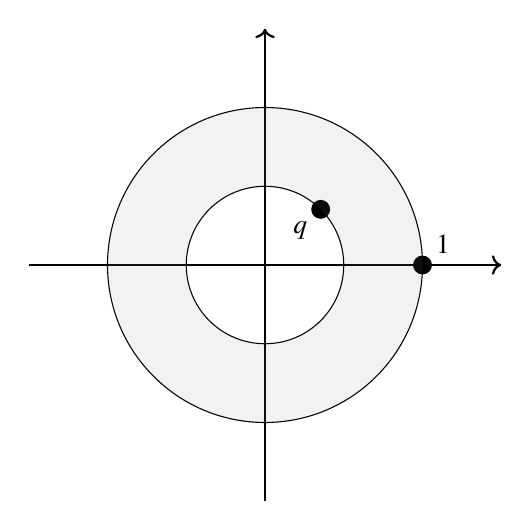
\begin{tikzpicture}[baseline=(current bounding box.center)]
% http://tex.stackexchange.com/questions/202607/drawing-discs-with-circular-holes-with-tikz
    \begin{scope}[thick,font=\scriptsize][set layers]
    \draw [->] (-3,0) -- (3,0);
    \draw [->] (0,-3) -- (0,3);
    \end{scope}
    \draw[solid] (0,0) circle (1);
    \draw[solid] (0,0) circle (2);
    \fill (2,0) circle (0.12) ++(0.26,0.26) node {$1$};
    \fill (0.707,0.707) circle (0.12) ++(-0.26,-0.26) node {$q$};
    \path [draw=none, fill=gray, even odd rule, fill opacity = 0.1] (0,0) circle (2) (0,0) circle (1);
\end{tikzpicture}
\quad \quad $\rightsquigarrow$ \quad \quad
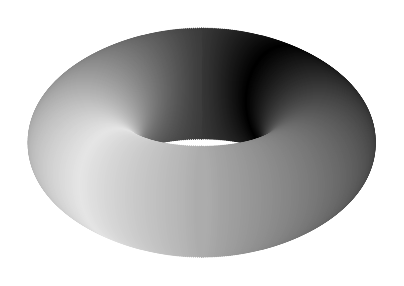
\begin{tikzpicture}[baseline=(current bounding box.center)]
% http://www.texample.net/tikz/examples/smooth-maps/
    \foreach \x in {90,89,...,-90} { % change 89 to 80 or 45 for speed
    % \elrad is the x-radius of the ellipse (technically, a circle seen
    % from side on at angle \x).  The 'max' is because at small angles
    % then the real ellipse is too thin and the torus doesn't ``fill
    % out'' nicely.
    \pgfmathsetmacro\elrad{20*max(cos(\x),.1)}
    % We draw the torus from the back to the front to get the right
    % layering effect.  To tint it, we define colours according to the
    % angle, but need different colours for the left and right pieces.
    % It'd be nice if the xcolor colour specification could take something
    % computed by pdfmath, such as {red!\tint} but it doesn't appear to
    % work, so we define the colours explicitly.
    \pgfmathsetmacro\ltint{.9*abs(\x-45)/180}
    \pgfmathsetmacro\rtint{.9*(1-abs(\x+45)/180)}
    \definecolor{currentcolor}{rgb}{\ltint, \ltint, \ltint}
    % This draws the right-hand circle.
    \draw[color=currentcolor,fill=currentcolor] 
        (xyz polar cs:angle=\x,y radius=.75,x radius=1.5) 
        ellipse (\elrad pt and 20pt);
    % This sets the colour correctly for the left-hand circle ...
    \definecolor{currentcolor}{rgb}{\rtint, \rtint, \rtint}
    % ... and draws it
    \draw[color=currentcolor,fill=currentcolor] 
        (xyz polar cs:angle=180-\x,radius=.75,x radius=1.5) 
        ellipse (\elrad pt and 20pt);
    % End of foreach statement
    }
\end{tikzpicture}
\end{center}
\caption{Presentation of an elliptic curve as the quotient of an annulus.}\label{AnnulusPicture}
\end{figure}

\begin{definition}
The basic $\theta$--function associated to $E_\Lambda$ is defined by \[\theta_q(u) = \prod_{m \ge 1} (1 - q^m) (1 + q^{m-\frac{1}{2}}u) (1 + q^{m-\frac{1}{2}}u^{-1}) = \sum_{n \in \Z} u^n q^{\frac{1}{2} n^2}.\]  Given two rational numbers $0 \le a, b \le 1$, we can also shift the zero-set of $\theta_q$ in the $1$ and $q$ directions by the fractions $a$ and $b$, giving translated $\theta$--functions: \[\theta_q^{a,b}(u) = \left(q^{\frac{a^2}{2}} \cdot u^a \cdot \exp(2 \pi i a b) \right) \cdot \theta_q(u q^a \exp(2 \pi i b)).\]
\end{definition}

The basic $\theta$--function vanishes on the set $\{\exp(2 \pi i (\frac{1}{2}m + \frac{\tau}{2}n))\}$, i.e., at the center of the fundamental annulus.  Since it has no poles, it cannot descend to give a function on $\C^\times / q^{\Z}$, and its failure to descend is witnessed by its imperfect periodicity relation: \[\theta_q(qu) = u^{-1} q^{\frac{-1}{2}} \theta_q(u).\]

\begin{lemma}[{\cite[Proposition 10.2.6]{Husemoller}}]
For any $N > 0$, define $V_q[N]$ to be the space of functions $f\co \C^\times \to \C$ satisfying \[f(q u) = u^{-N}  q^{-N^2/2} f(u).\]  Then, $V_q[N]$ has $\C$--dimension $N^2$, and the functions $\theta_q^{a, b}$ give a basis as $a$ and $b$ range over rational numbers with denominator $N$. \qed
\end{lemma}

Even though these functions do not themselves descend to $\C^\times / q^{\Z}$, we can collectively use them to construct a map to complex projective space, where the quasi-periodicity relations will mutually cancel in homogeneous coordinates.
\begin{theorem}[{\cite[Proposition 10.3.2]{Husemoller}}]
Consider the map
\begin{align*}
\C / (N \cdot \Lambda) & \xrightarrow{f_{(N)}} \P^{N^2-1}(\C), \\
z & \mapsto [\cdots : \theta_q^{i/N, j/N}(z) : \cdots].
\end{align*}
For $N > 1$, this map is an embedding. \qed
\end{theorem}

\begin{example}
Let us expand this in the case of $N = 2$.  The four functions involved are labeled $\theta_q^{0,0}$, $\theta_q^{0,1/2}$, $\theta_q^{1/2,0}$, and $\theta_q^{1/2,1/2}$, and we record their zero loci in \Cref{ThetaFunctionsTable}.  The image of $f_{(2)}$ in $\P^{2^2 - 1}(\C)$ is cut out by the equations
\begin{align*}
A^2 x_0^2 & = B^2 x_1^2 + C^2 x_2^2, &
A^2 x_3^2 & = C^2 x_1^2 - B^2 x_2^2,
\end{align*}
where
\begin{align*}
x_0 & = \theta_q^{0, 0}(u^2), &
x_1 & = \theta_q^{0, 1/2}(u^2), &
x_2 & = \theta_q^{1/2, 0}(u^2), &
x_3 & = \theta_q^{1/2, 1/2}(u^2)
\end{align*}
and
\begin{align*}
A & = \theta_q^{0, 0}(0) = \sum_n q^{n^2}, &
B & = \theta_q^{0, 1/2}(0) = \sum_n (-1)^n q^{n^2}, &
C & = \theta_q^{1/2, 0}(0) = \sum_n q^{(n + 1/2)^2},
\end{align*}
upon which there is the additional ``Jacobi'' relation \[A^4 = B^4 + C^4.\]
\end{example}

\begin{figure}
\begin{center}
\begin{tabular}{@{}cc@{}} \toprule
Function & Zero locus \\
\midrule
$\theta_q^{0,0}$ & $q^{\Z} \cdot q^{1/2} \cdot i$ \\
$\theta_q^{0,1/2}$ & $q^{\Z} \cdot q^{1/2}$ \\
$\theta_q^{1/2,0}$ & $q^{\Z} \cdot i$ \\
$\theta_q^{1/2,1/2}$ & $q^{\Z}$. \\ \bottomrule
\end{tabular}
\end{center}
\caption{Standard $\theta$--functions and their offsets}\label{ThetaFunctionsTable}
\end{figure}

\begin{remark}
This embedding of $E_\Lambda$ as an intersection of quadric surfaces in $\CP^3$ is quite different from the Weierstrass embedding.  Nonetheless, the embeddings are analytically related.  Namely, there is an equality \[\frac{d^2}{dz^2} \log \theta_q(u) = \wp_\Lambda(z).\]  Separately, Weierstrass considered a function $\sigma_\Lambda$, defined by \[\sigma_\Lambda(z) = z \prod_{\omega \in \Lambda \setminus 0} \left( 1 - \frac{z}{\omega} \right) \cdot \exp \left[ \frac{z}{\omega} + \frac{1}{2} \left( \frac{z}{\omega} \right)^2 \right],\] which also has the property that its second logarithmic derivative is $\wp$ and so is ``basically $\theta_q^{1/2,1/2}$''.  In fact, any elliptic function can be written in the form \[c \cdot \prod_{i=1}^n \frac{\sigma_\Lambda(z - a_i)}{\sigma_\Lambda(z - b_i)}.\]
\end{remark}

The $\theta$--functions version of the story has two main successes: it continues to make sense in algebraic geometry, without invoking transcendental functions, and in fact there is a version of this story for an \emph{arbitrary} abelian variety.  It turns out that all abelian varieties are projective, and the theorem sitting at the heart of this claim is
\begin{corollary}[{``Theorem of the Cube'', \cite[Corollary I.6.4 and Theorem I.7.1]{Milne}}]\label{Theta3IsTrivial}
Let $A$ be an abelian variety, let $p_i: A \times A \times A \to A$ be the projection onto the $i${\th} factor, and let $p_{ij} = p_i +_A p_j$, $p_{ijk} = p_i +_A p_j +_A p_k$.  Then for any invertible sheaf $\L$ on $A$, the sheaf \[\Theta^3(\L) := \frac{p_{123}^* \L \otimes p_1^* \L \otimes p_2^* \L \otimes p_3^* \L}{p_{12}^* \L \otimes p_{23}^* \L \otimes p_{31}^* \L \otimes p_\emptyset^* \L} = \bigotimes_{I \subseteq \{1, 2, 3\}} (p_I^* \L)^{(-1)^{|I| - 1}}\] on $A \times A \times A$ is trivial.  If $\L$ is rigid (i.e., it has a specified trivialization at the identity point of $A$), then $\Theta^3(\L)$ is \emph{canonically} trivialized by a section $s(A; \L)$. \qed
\end{corollary}

\begin{remark}
One way to read the Theorem of the Cube is that a weight zero divisor on an abelian variety is principal (i.e., it is the zeroes and poles of a meromorphic function) if and only if its nodes sum to zero.  The meromorphic function you construct this way is unique up to scale, so if you impose a normalization condition at the identity point, you get a unique such function.  Altogether, this gives a pairing between $(A \times A)^*$ and $A$, which can be reconsidered as a multiplication map $A \times A \to A$.
\end{remark}

\begin{remark}
The section $s(A; \L)$ satisfies three familiar properties:
\begin{itemize}
\item It is symmetric: pulling back $\Theta^3 \L$ along a shuffle automorphism of $A^3$ yields $\Theta^3 \L$ again, and the pullback of the section $s(A; \L)$ along this shuffle agrees with the original $s(A; \L)$ across this identification.
\item It is rigid: by restricting to $* \times A \times A$, the tensor factors in $\Theta^3 \L$ cancel out to give the trivial bundle over $A \times A$.  The restriction of the section $s(A; \L)$ to this pullback bundle agrees with the extension of the rigidifying section.
\item It satisfies a $2$--cocycle condition: in general, we define \[\Theta^k \L := \bigotimes_{I \subseteq \{1, \ldots, k\}} (p_I^* \L)^{(-1)^{|I| - 1}}.\]  In fact, $\Theta^{k+1} \L$ can be written as a pullback of $\Theta^k \L$: \[\Theta^{k+1} \L = \frac{(p_{12} \times \id_{A^{k-1}})^* \L}{(p_1 \times \id_{A^{k-1}})^* \L \otimes (p_2 \times \id_{A^{k-1}})^* \L},\] and pulling back a section $s$ along this map gives a new section \[(\delta s)(x_0, x_1, \ldots, x_k) := \frac{s(x_0 +_A x_1, x_2, \ldots, x_k)}{s(x_0, x_2, \ldots, x_k) \cdot s(x_1, x_2, \ldots, x_k)}.\]  Performing this operation on the first and second factors yields the defining equation of a $2$--cocycle.
\end{itemize}
\end{remark}

\begin{remark}
The proof of projectivity arising from this method rests on choosing a line bundle on $A$, extracting from it a very ample line bundle, and then constructing some generating global sections to get an embedding into $\P(\L^{\oplus n})$~\cite[Remark II.7.8.2]{Hartshorne}.  Mumford~\cite{MumfordEquationsI} showed that a choice of ``$\theta$--structure'' on $(A, \L)$, which is only slightly more data, gives a canonical choice of generating global sections as well as a canonical identification of $\P(\L^{\oplus n})$ with a \emph{fixed} projective space.  This is suitable for studying how these equations change as one considers different points in the moduli of abelian varieties~\cite{MumfordEquationsII,MumfordEquationsIII}.
\end{remark}

\begin{remark}[{\cite[Section 4]{Breen}}]
Breen presented a relative version of this story that applies to arbitrary \emph{commutative group schemes}, where the basic objects are a choice of line bundle $\L$ over a commutative group scheme $A$, a choice of trivialization of $\Theta^3 \L$, and an epimorphism $\pi\co A' \to A$ that trivializes $\L$.
\end{remark}

Finally, we remark that the function \[e\co C^3(\G; \Gm) \to \InternalHom{FormalGroups}(\G_a^{\sm 2}, \G_m)\] considered in \Cref{ChromaticKUCoopnsSection} also manifests in the theory of abelian varieties.  Let $A$ be an abelian variety equipped with a line bundle $\L$.  Suppose that $s$ is a symmetric, rigid section of $\Theta^3 \L$, sometimes called a \index{cubical structure}\textit{cubical structure on $\L$}.  Using the identification $(p_{12} - p_1 - p_2)^* \Theta^2 \L = \Theta^3 \L$, this induces the structure of a \index{symmetric biextension}\textit{symmetric biextension} on $\Theta^2 \L$ via the multiplication maps
\begin{align*}
(\Theta^2 \L)_{x, y} \otimes (\Theta^2 \L)_{x', y} & \to (\Theta^2 \L)_{x + x', y}, &
(\Theta^2 \L)_{x, y} \otimes (\Theta^2 \L)_{x, y'} & \to (\Theta^2 \L)_{x, y + y'}.
\end{align*}

\begin{definition}
There is a canonical piece of gluing data on this biextension, in the form of an isomorphism of pullback bundles
\begin{align*}
e_{p^j}\co (p^j \times 1)^* \L|_{A[p^j] \times A[p^j]} & \cong (1 \times p^j)^* \L|_{A[p^j] \times A[p^j]}, \\
(\ell, x, y) & \mapsto \left(\ell \cdot \prod_{k=1}^{p^j-1} \frac{s(x, [k]x, y)}{s(x, [k]y, y)} \right).
\end{align*}
This function $e_{p^j}$ is called the \index{Weil pairing}\textit{($p^j$){\th} Weil pairing}.
\end{definition}

\begin{figure}
\begin{center}
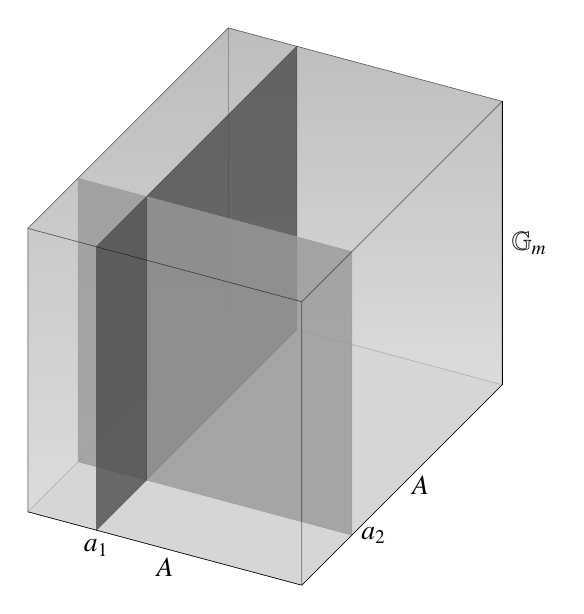
\begin{tikzpicture}[x  = {(-0.707cm,-0.707cm)},
                    y  = {(0.9659cm,-0.25882cm)},
                    z  = {(0cm,1cm)},
                    scale = 1.8,
                    color = {lightgray}]
% style of faces
\tikzset{facestyle/.style={fill=black!25,draw=black,very thin,line join=round,opacity=.4},slicestyle/.style={fill=black!25,draw=black,very thin,line join=round,opacity=.8}}
%\tikzset{facestyle/.style={fill=cyan,draw=blue,very thin,line join=round,opacity=.4},slicestyle/.style={fill=cyan,draw=blue,very thin,line join=round,opacity=.7}}
% face "back" 
\begin{scope}[canvas is zy plane at x=0]
  \path[facestyle,shade] (0,0) rectangle (2,2);
\end{scope}
% face  "left"
\begin{scope}[canvas is zx plane at y=0]
  \path[facestyle,shade] (0,0) rectangle (2,2);
\end{scope}
% face "down"
\begin{scope}[canvas is yx plane at z=0]
  \path[facestyle,color=lightgray] (0,0) rectangle (2,2);
\end{scope}
% face "red slice back"
\begin{scope}[canvas is zy plane at x=1.5]
  \path[slicestyle,color=black!50] (0,0) rectangle (2,0.5);
\end{scope}
% face "green slice back"
\begin{scope}[canvas is zx plane at y=0.5]
  \path[slicestyle,color=black] (0,0) rectangle (2,1.5);
\end{scope}
% face "red slice front"
\begin{scope}[canvas is zy plane at x=1.5]
  \path[slicestyle,color=black!50] (0,0.5) rectangle (2,2);
\end{scope}
% face "green slice front"
\begin{scope}[canvas is zx plane at y=0.5]
  \path[slicestyle,color=black] (0,1.5) rectangle (2,2);
\end{scope}
% face "front"
\begin{scope}[canvas is zy plane at x=2]
  \path[facestyle] (0,0) rectangle (2,2);
\end{scope}
% face  "right"
\begin{scope}[canvas is zx plane at y=2]
  \path[facestyle] (0,0) rectangle (2,2);
\end{scope}
% face "up" 
\begin{scope}[canvas is yx plane at z=2]
  \path[facestyle] (0,0) rectangle (2,2);
\end{scope}
% labels
\draw[very thin,black,line join=round]
     (2,0,0) -- node [below,black] {$A$} (2,2,0);
\draw[very thin,black,line join=round]
     (2,2,0) -- node [right,black] {$A$} (0,2,0);
\draw[very thin,black,line join=round]
     (0,2,0) -- node [right,black] {$\Gm$} (0,2,2);
\draw[very thin,black,line join=round]
     (2,0.5,0) -- node [below,black] {$a_1$} (2,0.5,0);
\draw[very thin,black,line join=round]
     (1.5,2,0) -- node [right,black] {$a_2$} (1.5,2,0);
\end{tikzpicture}
\hspace{0.5em}
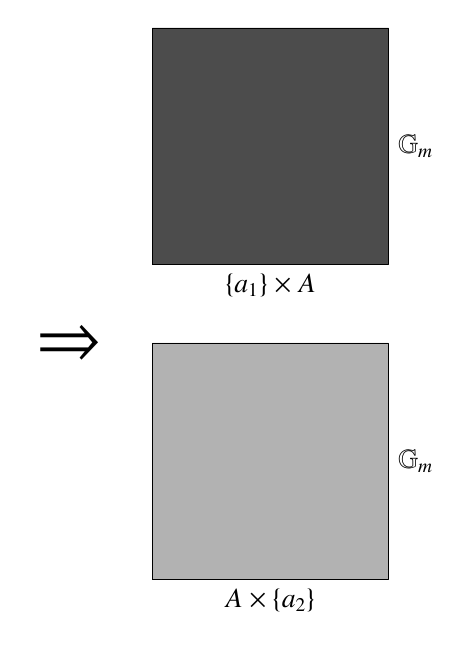
\begin{tikzpicture}
    \draw[very thin,black,line join=round,fill=black!30]
        (0,1) -- node [below,black] {$A \times \{a_2\}$} (3,1) -- node[right,black] {$\Gm$} (3,4) -- (0,4) -- (0,1);
    \draw[very thin,black,line join=round,fill=black!70]
        (0,5) -- node [below,black] {$\{a_1\} \times A$} (3,5) -- node[right,black] {$\Gm$} (3,8) -- (0,8) -- (0,5);
    \node[anchor=east] at (-0.5,4) {\Huge $\Rightarrow$};
\end{tikzpicture}
\end{center}
\caption{Extensions contained in a biextension.}
\end{figure}

\begin{remark}
In the case that $A$ is an elliptic curve, this agrees with the usual definition of its ``Weil pairing''.  In the case of a \emph{complex} elliptic curve $\C / (1, \tau)$, this degenerates further to the assignment \[\left( \frac{a}{n}, \frac{b}{n} \tau \right) \mapsto \exp\left(-2\pi i \frac{ab}{n}\right).\]
\end{remark}

We now actually leverage this arithmetic geometry by placing ourselves in a situation where algebraic topology is directly linked to abelian varieties.

\begin{definition}\label{DefnEllipticSpectrum}
An \index{elliptic spectrum}\textit{elliptic spectrum} consists of a even--periodic ring spectrum $E$, a (generalized) elliptic curve $C$ over $\Spec E_0$, and a fixed isomorphism \[\phi\co C^\wedge_0 \xrightarrow{\cong} \CP^\infty_E.\]  A map among such spectra consists of a map of ring spectra $f\co E \to E'$ together with a specified isomorphism of elliptic curves $\psi\co f^* C \to C'$.\footnote{Elliptic curves and cohomology theories can be brought much closer together still, as in Lurie's framework~\cite[Sections 4 and 5.3]{LurieSurveyOfEll}.}
\end{definition}

\begin{remark}
Our preference for \emph{isomorphisms} of elliptic curves rather than general homomorphisms is prompted by our study of stable operations: we have seen that a stable operation between complex-oriented ring spectra can only ever give rise to an isomorphism of formal group laws (incorporating a suitable base change).  More broadly, we have also found that the collection of possible isomorphisms of formal group laws organizes into the \index{context!stable}\textit{stable context}, a very important object in our study.  In the next Case Study, we will develop a theory (with an attendant notion of context) which incorporates \emph{isogenies} of elliptic curves in addition to isomorphisms.
\end{remark}

Coupling \Cref{DefnEllipticSpectrum} to \Cref{BU6Triumvirate} and \Cref{Theta3IsTrivial}, we conclude the following:
\begin{corollary}\label{EllipticSpectraAreOriented}
An elliptic spectrum $(E, C, \phi)$ receives a canonical map of ring spectra \[MU[6, \infty) \to E.\]  This map is natural in choice of elliptic spectrum: if $(E, C, \phi) \to (E', C', \phi')$ is a map of elliptic spectra, then the triangle
\begin{center}
\begin{tikzcd}
& MU[6, \infty) \arrow{ld} \arrow{rd} \\
E \arrow{rr} & & E'
\end{tikzcd}
\end{center}
commutes. \qed
\end{corollary}

\begin{example}
Our basic example of an elliptic curve was $E_\Lambda = \C / \Lambda$, with $\Lambda$ a complex lattice.  The projection $\C \to \C / \Lambda$ has a local inverse which defines an isomorphism of formal groups \[\phi\co (E_\Lambda)^\wedge_0 \xrightarrow{\cong} \G_a \times \Spec \C,\] as well as an isomorphism of cotangent spaces
\begin{center}
\begin{tikzcd}
T^0 (E_\Lambda)^\wedge_0 \arrow[iso]{r} \arrow[iso, leftarrow]{d} & \C \arrow[equal]{d} \\
T^0 (\G_a \times \Spec \C) \arrow[iso]{r} & \C.
\end{tikzcd}
\end{center}
Accordingly, we define an elliptic spectrum $HE_\Lambda P$ whose underlying ring spectrum is $H\C P$ and whose associated elliptic curve and isomorphism are $E_\Lambda$ and $\phi$.  This spectrum receives a natural map \[MU[6, \infty) \to HE_\Lambda P,\] which to a bordism class $M \in MU[6, \infty)_{2n}$ assigns an element $\Phi_\Lambda(M) \cdot u_\Lambda^n \in HE_\Lambda P_{2n}$, where $u_\Lambda$ is the canonical section of $\widetilde{\pi_2 HE_\Lambda P} = \omega_{\CP^\infty_{HE_\Lambda P}}$ and $\Phi_\Lambda(M) \in \C$ is some resulting complex number.
\end{example}

\begin{example}
The naturality of the $MU[6, \infty)$--orientation moves us to consider more than one elliptic spectrum at a time.  If $\Lambda'$ is another lattice with $\Lambda' = \lambda \cdot \Lambda$, then the multiplication map $\lambda\co \C \to \C$ descends to an isomorphism $E_\Lambda \to E_{\Lambda'}$ and hence a map of elliptic spectra $HE_{\Lambda'}P \to HE_\Lambda P$ acting by $u_{\Lambda'} \mapsto \lambda u_\Lambda$.  The commuting triangle in \Cref{EllipticSpectraAreOriented} then begets the \emph{modularity relation} \[\Phi(M; \lambda \cdot \Lambda) = \lambda^{-n} \Phi(M; \Lambda).\]
\end{example}

\begin{example}\label{OrdinaryHomologyInUpperHalfPlaneEx}
This equation leads us to consider all curves $E_\Lambda$ simultaneously---or, equivalently, to consider modular forms.  The lattice $\Lambda$ can be put into a standard form, by picking a basis and scaling it so that one vector lies at $1$ and the other vector lies in the upper half-plane.  This gives a cover \[\h \to \moduli{ell} \times \Spec \C\] which is well-behaved (i.e., unramified) away from the special points $i$ and $e^{2 \pi i / 6}$.  A \index{modular form}\textit{complex modular form of weight $n$} is an analytic function $\h \to \C$ which satisfies a certain decay condition and which is quasi-periodic for the action of $SL_2(\Z)$, i.e.,\footnote{That is, for the action of change of basis vectors.} \[f\left(M; \frac{a \tau + b}{c \tau + d} \right) = (c \tau + d)^n f(M; \tau).\]

Using these ideas, we construct a cohomology theory $H \sheaf O_{\h} P$, where $\sheaf O_{\h}$ is the ring of complex-analytic functions on the upper half-plane.  The $\h$--parametrized family of elliptic curves \[\h \times \C / (1, \tau) \to \h,\] together with the logarithm, present $H \sheaf O_{\h} P$ as an elliptic spectrum $H\h P$.  The canonical map $\Phi\co MU[6, \infty) \to H\h P$ specializes at a point to give the functions $\Phi(-; \Lambda)$ considered above, and hence $\Phi(M) \in u^k \cdot \sheaf O_{\h}$ is itself a complex modular form of weight $k$.
\end{example}

In fact, this totalized map $\Phi$ is a ghost of Ochanine and Witten's modular genus from \Cref{OchanineWittenTheorem}, as a bordism class in $MU[6, \infty)_{2n}$ is, in particular, a bordism class in $M\String_{2n}$.  However, they know more about this function than we can presently see: for instance, they claim that it has an integral $q$--expansion.  In terms of the modular form, its $q$--expansion is given by building the Taylor expansion ``at $\infty$'' (using that unspoken decay condition).  In order to use our topological methods, it would be nice to have an elliptic spectrum embodying these $q$--expansions in the same way that $H\h P$ embodied holomorphic functions, together with a comparison map that trades a modular form for its $q$--expansion.  The main ideas leading to such a spectrum come from considering the behavior of $E_\Lambda$ as $\tau$ tends to $i \cdot \infty$.

\begin{definition}
Note that as $\tau$ tends to $i \cdot \infty$, the parameter $q = \exp(2 \pi i \tau)$ tends to $0$.  In the multiplicative model of \Cref{SectionEllipticCurvesAndThetaFunctions}, we considered the punctured complex disk $D'$ with its associated family of elliptic curves \[C'_{\mathrm{an}} = \C^\times \times D' / (u, q) \sim (qu, q).\]  The fiber of $C'$ over a particular point $q \in D'$ is the curve $\C^\times / q^{\Z}$. %  , and $\theta$ determines a holomorphic function on the total space $\C^\times \times D'$.
The Weierstrass equations give an embedding of $C'_{\mathrm{an}}$ into $D' \times \CP^2$ described by \[wy^2 + wxy = x^3 - 5 \alpha_3 w^2 x + -\frac{5 \alpha_3 + 7 \alpha_5}{12}w^3\] for certain functions $\alpha_3$ and $\alpha_5$ of $q$.\footnote{Indeed, certain modular forms: $\alpha_3$ has weight $6$ and $\alpha_5$ has weight $10$.}  At $q = 0$, this curve collapses to the twisted cubic \[wy^2 + wxy = x^3,\] and over the whole open unit disc $D$ we call this extended family $C_{\mathrm{an}}$.

Now let $A \subseteq \Z\ps{q}$ be the subring of power series which converge absolutely on the open unit disk.  It turns out that the coefficients of the Weierstrass cubic (i.e., $5\alpha_3$ and $\frac{1}{12}(5\alpha_3+7\alpha_5)$) lie in $A$, so it determines a generalized elliptic curve $C$ over $\Spec A$, and $C_{\mathrm{an}}$ is the curve given by base-change from $A$ to the ring of holomorphic functions on $D$~\cite[Section 5]{MoravaFormsOfKthy}.  The \index{elliptic curve!Tate curve}\textit{Tate curve} is the intermediate family $C_{\Tate}$ over the intermediate base $D_{\Tate} = \Spec \Z\ps{q}$, as base-changed from $A$.
\end{definition}

The singular fiber at $q = 0$ prompts us to enlarge our notion of elliptic curve slightly.

\begin{definition}[{\cite[Definitions B.1-2]{AHSTheoremOfTheCube}}]
A \index{elliptic curve!Weierstrass curve}\textit{Weierstrass curve} is \emph{any} curve of the form \[C(a_1, a_2, a_3, a_4, a_6) := \left\{ [x : y : w] \in \mathbb P^2 \middle| \begin{array}{c} y^2 w + a_1 xyw + a_3 yw^2 = \\ x^3 + a_2 x^2 w + a_4 x w^2 + a_6 w^3 \end{array} \right\}.\]  A \index{elliptic curve!generalized}\textit{generalized elliptic curve} over $S$ is a scheme $C$ equipped with maps \[S \xrightarrow{0} C \xrightarrow{\pi} S\] such that $C$ is Zariski--locally isomorphic to a system of Weierstrass curves (in a way preserving $0$ and $\pi$).\footnote{An elliptic curve in the usual sense turns out to be a generalized elliptic curve which is smooth, i.e., the discriminant of the Weierstrass equations is a unit.}\footnote{Unfortunately, ``generalized elliptic curve'' already means something in number theory, but Ando, Hopkins, and Strickland reused this phrase for this definition in their published article.  In a number theorist's language, these are ``stable curves of genus $1$ with specified section in the smooth locus''.  No adjective other than ``generalized'' seems to be much better: singular, for instance, evokes the right idea but is also already taken.}
\end{definition}

\begin{remark}[{\cite[pg.\ 670]{AHSTheoremOfTheCube}}]\label{TwistedCubicGivesGm}
The singularities of a degenerate Weierstrass equation always occur outside of a formal neighborhood of the marked identity point, which in fact still carries the structure of a formal group.  The formal group associated to the twisted cubic is the formal multiplicative group (indeed, the smooth locus of the twisted cubic \emph{is the multiplicative group}), and the isomorphism making the identification extends a family of such isomorphisms $\phi$ over the nonsingular part of the Tate curve.
\end{remark}

\begin{definition}[{\cite[Section 5]{MoravaFormsOfKthy}, \cite[Section 2.7]{AHSTheoremOfTheCube}}]
The generalized elliptic spectrum $K_{\Tate}$, called \index{Tate K theory@Tate $K$--theory}\textit{Tate $K$--theory}, has as its underlying spectrum $KU\ps{q}$.  The associated generalized elliptic curve is $C_{\Tate}$, and the isomorphism $\CP^\infty_{KU\ps{q}} \cong (C_{\Tate})^\wedge_0$ is $\phi$ from \Cref{TwistedCubicGivesGm}.
\end{definition}

\noindent The trade for the breadth of this definition is that theorems pulled from the study of abelian varities have to be shown to extend uniquely to those generalized elliptic curves which are not smooth curves.

\begin{theorem}[{\cite[Propositions 2.57 and B.25]{AHSTheoremOfTheCube}}]\label{GeneralizedTheta3IsTrivial}
For a generalized elliptic curve $C$, there is a canonical\footnote{Canonical, with a unique continuous extension from the smooth bulk of the moduli of generalized elliptic curves, but \emph{not} actually unique over the singular locus.} trivialization $s$ of $\Theta^3 \sheaf I(0)$ which is compatible with change of base and with isomorphisms.  If $C$ is a smooth elliptic curve, then $s$ agrees with that of \Cref{Theta3IsTrivial}. \qed
\end{theorem}

\begin{corollary}\label{D3thetaTrivializes}
The trivializing section $s$ associated to $C_{\Tate}$ is given by $\delta^{\circ 3} \tilde \theta$, where $\tilde \theta_q$ is a slight modification of the classical $\theta$--function:
\begin{align*}
\tilde \theta_q(u) & = (1 - u)\prod_{n > 0}(1 - q^n u)(1 - q^n u^{-1}), &
\tilde \theta_q(qu) & = -u^{-1} \tilde\theta_q(u).
\end{align*}
\end{corollary}
\begin{proof}
Even though $\tilde \theta$ is not a function on $C_{\Tate}$ because of its quasiperiodicity, it does trivialize both $\pi^* \sheaf I(0)$ for $\pi\co \C^\times \times D \to C_{\Tate}$ and $\sheaf I(0)$ for $(C_{\Tate})^\wedge_0$.  Moreover, the quasiperiodicities in the factors in the formula defining $\delta^3 \tilde \theta|_{(C_{\Tate})^\wedge_0}$ cancel each other out, and the resulting function \emph{does} descend to give a trivialization of $\Theta^3 \sheaf I(0)$.  By the unicity and continuity clauses in \Cref{GeneralizedTheta3IsTrivial}, it must give a formula expressing $s$.
\end{proof}

\begin{definition}
The induced map \[\sigma_{\Tate}\co MU[6, \infty) \to K_{\Tate}\] is called the \index{sigma orientation@$\sigma$--orientation}\textit{complex $\sigma$--orientation}.
\end{definition}

\begin{corollary}\label{WittensTheoremForBU6}
Let $M \in \pi_{2n} MU[6, \infty)$ be a bordism class.  The $q$--expansion of Witten's modular form $\Phi(M)$ has integral coefficients.
\end{corollary}
\begin{proof}
The span of elliptic spectra equipped with $MU[6, \infty)$--orientations
\begin{center}
\begin{tikzcd}
& MU[6, \infty) \arrow["\Phi"]{rd} \arrow{d} \arrow["\sigma_{\Tate}"']{ld} \\
K_{\Tate} \arrow{r} & K_{\Tate} \otimes \C & H\h P \arrow{l}
\end{tikzcd}
\end{center}
models $q$--expansion.  The arrow $K_{\Tate} \to K_{\Tate} \otimes \C$ is injective on homotopy, which shows that the $q$--expansion of $\Phi(M)$ lands in the subring of integral power series.
\end{proof}

We can use the formula $\sigma_{\Tate} = \delta^3 \tilde \theta$ appearing in \Cref{D3thetaTrivializes} to explicitly understand the genus associated to $\sigma_{\Tate}$ by passing to homotopy groups.  To begin, the appearances of the map $\delta$ in \Cref{BUtoBUZ}, \Cref{BSUToBU}, and \Cref{MSUToMU6} show that $\sigma_{\Tate}$ belongs to the commutative triangle
\begin{center}
\begin{tikzcd}
MU[6, \infty) \arrow["\delta"]{r} \arrow["\sigma_{\Tate}"']{drrr} & MSU \arrow["\delta"]{r} & MU \arrow["\delta"]{r} & MUP \arrow["\tilde \theta"]{d} \\
& & & KU\ps{q}.
\end{tikzcd}
\end{center}
We will analyze this triangle by comparing $\tilde\theta$ to the usual $MUP$--orientation of $KU$, which selects the coordinate $f(u) = 1 - u$ on the formal completion of $\Gm = \Spec \Z[u^\pm]$.  Appealing to \Cref{BUtoBUZ}, the induced $MU$--orientation \[MU \xrightarrow{\delta} MUP \xrightarrow{\Td} KU\] sends $f$ to the rigid section $\delta f$ of \[\Theta^1 \sheaf I(0) = \sheaf I(0)_0 \otimes \sheaf I(0)^{-1} \cong \omega \otimes \sheaf I(0)\] given by \[\delta f = \frac{1}{1 - u} \left( - \frac{du}{u} \right).\]  The difference between $\delta \Td$ and $\delta \tilde\theta$ is expressed by an element $\psi \in C^1(\widehat C_{\Tate}; \Gm)$, given explicitly by the quotient formula \[\psi = \left(\frac{\Td(1)}{\Td(u)}\right)^{-1} \cdot \frac{\tilde \theta_q(1)}{\tilde \theta_q(u)} = \prod_{n \ge 1} \frac{(1 - q^n)^2}{(1 - q^n u)(1 - q^n u^{-1})}.\]  This gives a re-expression of $\delta \tilde\theta$ as the composite \[\delta \tilde\theta\co MU \xrightarrow{\eta_R} MU \sm MU \simeq MU \sm BU_+ \xrightarrow{\delta\Td \sm \psi} K_{\Tate},\] and hence its effect on a line bundle is determined by the evaluation of this characteristic series: \[\psi(1 - \L) = \prod_{n \ge 1} \frac{(1 - q^n)^2}{(1 - q^n \L)(1 - q^n \L^{-1})}.\]  Its effect on vector bundles in general is determined by the splitting principle and an exponential law, which after some computation~\cite[Section 2.7]{AHSTheoremOfTheCube} gives the generic formula \[\psi(\dim V \cdot 1 - V) = \bigotimes_{n \ge 1} \bigoplus_{j \ge 0} \Sym^j(\dim V \cdot 1 - V \otimes_{\R} \C) q^{jn} =: \bigotimes_{n \ge 1} \Sym_{q^n}(- \bar V_{\C}).\]  Finally, the map $(\eta_R)_*\co MU_* \to \pi_*(MU \sm \Susp^\infty_+ BU)$ sends a manifold $M$ with stable normal bundle $\nu$ to the pair $(M, \nu)$, so we at last compute
\begin{align*}
\sigma_{\Tate}(M \in \pi_{2n} MU[6, \infty)) & = (\delta \Td \sm \theta')(M, \nu) \\
& =: \Td\left(M; \bigotimes_{n \ge 1} \Sym_{q^n}(\bar \tau_{\C}) \right).
\end{align*}
This is exactly Witten's formula for his genus, as applied to complex manifolds with first two Chern classes trivialized.

\begin{remark}[{\cite[Section 1.5]{RezkFelixKlein}}]
Witten defines his characteristic series for \emph{oriented} manifolds by the formula
\begin{align*}
K_{\mathrm{Witten}}(x) & = \exp\left( \sum_{k=2}^\infty 2 G_{2k}(\tau) \cdot \frac{x^{2k}}{(2k)!} \right) \\
& = \frac{x/2}{\sinh(x/2)} \cdot \left(\prod_{n=1}^\infty \frac{(1 - q^n)^2}{(1 - q^n u)(1 - q^n u^{-1})}\right) \cdot e^{-G_2(\tau) x^2},
\end{align*}
where $G_{2k}$ is the $2k${\th} Eisenstein series.  Noting that $G_2$ is \emph{not} a modular form, the condition that $p_1(M) / 2$ vanish is precisely the condition that $G_2$ contribute nothing to the sum, so that the remainder \emph{is} a modular form.
\end{remark}

\begin{remark}[{\cite{AndoMorava}}]
Another location where this series $\psi$ appears is in the theory of Tate $p$--divisible groups of Ando and Morava (and, in some sense, in the sense of Katz and Mazur).  For a formal group $\G$ over $\Spf R$ with group law $+_\phi$, they consider the Weierstrass product \[\Theta_{\phi}(x; q) = x \cdot \prod_{\substack{k \in \Z \\ k \ne 0}} \frac{(x +_\phi [k]_\phi(q))}{[k]_\phi(q)} \in R\ps{x,q},\] which plays the role of a kind of $\theta$--function for $\G$.  They also connect this series the quotient function mapping to the group scheme $\G / q^{\Z}$ (in the sense of \Cref{NormForFns}), which they further identify as the universal extension of $\G$ by a constant $p$--divisible group of dimension $1$.  In the presense of a global object $\mathbb G$ specializing to $\G$ (as in the case of $\G_a$ or $\G_m$), they show how to modify this product to an analytically convergent power series, recovering the characteristic series for the $\widehat A$--genus and the $L$--genus.  The higher height analogues of these results seem very mysterious and very interesting.\footnote{Morava is generally full of interesting ideas about genera---see, for instance,~\cite{MoravaMotivicThomIso}.}
\end{remark}

\begin{remark}[{\cite{AFG}}]
Ando, French, and Ganter have given a construction that convert $MU[2k, \infty)$--orientations of a spectrum $E$ to $MU[2(k-1), \infty)$--orientations of the pro-spectrum $E^{\CP^\infty_{-\infty}}$.  Performing this operation to the $\sigma$--orientation of $K^{\Tate}$ gives the ``two--variable Jacobi genus'', which assigns $SU$--manifolds to certain classes in $\pi_0 (K^{\Tate})^{\CP^\infty_{-\infty}} = \Z\ps{q}(\!(y)\!)$ connected to meromorphic Jacobi forms.
\end{remark}













\section{Chromatic \texorpdfstring{$\Spin$}{Spin} and \texorpdfstring{$\String$}{String} orientations}

We now turn to understanding $M\String$--orientations in turns of $MU[6, \infty)$--orientations.  We will approach this in successive passes, keeping the desired picture sharp the entire time but introducing generality slowly.  Unfortunately, most of the original source material~\cite{HAS,StricklandFSKS} for this has not been published, and hence it is difficult to give references.\footnote{Versions of some of this have appeared in work of Kitchloo and Laures~\cite{KitchlooLaures}.}  We have gone to some lengths to prepare the reader for the sorts of arguments that appear here: they are not so different from the arguments appearing elsewhere in this chapter.

We begin at the maximally simple situation, where $2$ is inverted.  In this case, the Wood cofiber sequence \[\Susp kO \xrightarrow{\eta} kO \xrightarrow{c} kU \xrightarrow{\lambda} \Susp^2 kO\] becomes split, since $\eta$ is a $2$--torsion element.  By considering different underlying infinite-loopspaces, this gives a number of identifications:
\begin{center}
\begin{tikzcd}[row sep=0em]
\OS{(-)}{0}: & BO \times \Z \arrow{r} & BU \times \Z \arrow{r} & \OS{kO}{2}, \\
\OS{(-)}{2}: & \OS{kO}{2} \arrow{r} & BU \arrow{r} & \OS{kO}{4}, \\
\OS{(-)}{4}: & \OS{kO}{4} \arrow{r} & BSU \arrow{r} & \OS{kO}{6}, \\
\OS{(-)}{6}: & \OS{kO}{6} \arrow{r} & BU[6, \infty) \arrow{r} & B\String.
\end{tikzcd}
\end{center}
Next, by recognizing $c\co kO \to kU$ as the complexification map, we note that it lies in fixed points for complex-conjugation on $kU$.  The other gain that inverting $2$ gets us is an idempotent selecting this fixed point subspectrum: there are a pair of orthogonal idempotents
\begin{align*}
P_+ & = \frac{1 + \xi}{2}, &
P_- & = \frac{1 - \xi}{2},
\end{align*}
which reidentify the splitting $kU \simeq kO \vee \Susp^2 kO$ in various equivalent ways: \[kU \simeq kO \vee \Susp^2 kO \simeq \im P_- \vee \im P_+ \simeq \ker P_+ \vee \ker P_- \simeq \left( \frac{kU}{\im P_+} \right) \vee \left( \frac{kU}{\im P_-} \right).\]  This last identification immediately gives access to the following result:
\begin{lemma}
For $E$ a complex-orientable ring spectrum with $1/2 \in \pi_0 E$, we have
\begin{align*}
B\String_E & = C_3(\CP^\infty_E) / ([a, b, c] = -[-a, -b, -c]), \\
\Spec E_0 B\String & = \left\{ f \in C^3(\CP^\infty_E; \Gm) \middle| f(a, b, c) = \frac{1}{f(-a, -b, -c)} \right\} \subseteq C^3(\CP^\infty_E; \Gm).
\end{align*}
\end{lemma}
\begin{proof}[Proof sketch]
This is a matter of translating the splittings above across \Cref{BU6Triumvirate}.  The complex-conjugation map $\xi$ acts on $C_k(\G)$ according to \[\xi[a_1, \ldots, a_n] = (-1)^n [-a_1, \ldots, -a_n],\] which encodes $B\String_E$ as the quotient of $BU[6, \infty)_E$ by $\im P_-$.  Finally, the claim about the homological scheme follows from the description of the cohomological formal scheme by Cartier duality.
\end{proof}

The repeated appearances of the terms in the above splittings suggest that the composite \[\tau\co kU \xrightarrow{\lambda} \Susp^2 kO \xrightarrow{\Susp^2 c} \Susp^2 kU\] of the maps in two adjacent cofiber sequences itself plays an interesting role.  This is the map that encodes surjecting onto one factor in the preceding splitting, then reincluding it into the next splitting.
\begin{lemma}
At the level of formal schemes, the map $\tau$ acts by
\begin{align*}
\tau\co C_k(\G) & \to C_{k+1}(\G) \\
[a_1, \ldots, a_k] & \mapsto [a_1, \ldots, a_k, -(a_1 + \cdots + a_k)].
\end{align*}
\end{lemma}
\begin{proof}
We are in pursuit of the following calculation in $kU^* (\CP^\infty)^{\times (k+1)}$ encoding complexification after decomplexification:
\begin{align*}
\beta^k x_1 \cdots x_k + \beta^k \overline{x_1} \cdots \overline{x_k} & = (1 - \L_1) \cdots (1 - \L_k) + (1 - \overline \L_1) \cdots (1 - \overline \L_k) \\
& = (1 - \L_1) \cdots (1 - \L_k) + \overline \L_1 \cdots \overline \L_k (\L_1 - 1) \cdots (\L_k - 1) \\
& = (1 - \L_1) \cdots (1 - \L_k) (1 - (-1)^{k+1} \overline \L_1 \cdots \overline \L_k) \\
& = \beta^{k+1} x_1 \cdots x_k \cdot \xi^* \mu^*(x_1, \ldots, x_k). \qedhere
\end{align*}
\end{proof}
Still in the case where $E$ is local away from $2$, we can use this alternative description of the inclusion of the $P_-$ factor to deduce an alternative description of the formal scheme associated to $B\String$:
\begin{corollary}
For $E$ a complex-orientable ring spectrum with $1/2 \in \pi_0 E$, we have
\begin{align*}
B\String_E & = C_3(\CP^\infty_E) / ([a, b, -a-b] = 0), \\
\Spec E_0 B\String & = \left\{ f \in C^3(\CP^\infty_E; \Gm) \middle| f(a, b, -a-b) = 1 \right\} \subseteq C^3(\CP^\infty_E; \Gm). \qed
\end{align*}
\end{corollary}

\begin{definition}
We denote this last functor by $\Sigma^3(\CP^\infty_E; \Gm)$, and more generally if $\L$ is a line bundle on $\CP^\infty_E$ then $\Sigma^3(\CP^\infty_E; \L)$ will denote the subscheme of $C^3(\CP^\infty_E; \L)$ of those trivializations which restrict to the rigidifying trivialization of $\Theta^3 \L$ on the subscheme of $(\CP^\infty)^{\times 3}$ specified by $[a, b, -a-b]$.  Such trivializations are referred to as \index{Sigma structure@$\Sigma$--structure}\textit{$\Sigma$--structures on $\L$}, following Breen~\cite[Section 5]{Breen}.
\end{definition}

\begin{corollary}\label{OddPrimaryMStringTriumvirate}
For $E$ a complex-orientable ring spectrum with $1/2 \in \pi_0 E$, the functor $\Sigma^3(\CP^\infty_E; \sheaf I(0))$ is isomorphic to the affine scheme $\Spec E_0 M\String$.  Moreover, the $E_0$--points of this scheme biject with ring spectrum maps $M\String \to E$. \qed
\end{corollary}

\begin{remark}[{\cite[Section 26.1]{Hirzebruch}}]
One of the most pleasant features of the case where $2$ is inverted is that real orientations can not only be identified, but the projection idempotents mean that they can be \emph{crafted} from complex orientations, and the idempotents have a recognizable effect on the traditional mechanisms for specifying orientations.  For instance, the Conner--Floyd orientation on $K$--theory is specified by the classical logarithm, and the associated real orientation formed by projection to the positive idempotent has logarithm \[\operatorname{tanh}^{-1}(x) = \frac{-\ln(1 - x) + \ln(1 + x)}{2},\] i.e., the average of the logarithm and its conjugate.  The resulting orientation is commonly referred to as the \index{orientation!Atiyah Bott Shapiro@Atiyah--Bott--Shapiro}\textit{Atiyah--Bott--Shapiro orientation}, whose associated genus is the \index{A hat genus@$\widehat A$--genus}\textit{$\widehat A$--genus}.  Similar techniques give access to connective real orientations associated to preexisting connective complex orientations.
\end{remark}

We now turn to the \emph{much} more complicated setting where $2$ is not invertible, where we again aim to identify $M\String$--orientations of a complex-orientable cohomology theory with certain $\Sigma$--structures.  This is not possible in much generality, a situation which is hinted by the analogous lower-order case: complex-orientability is flatly \emph{not enough} to conclude anything about whether a cohomology theory admits an $MO$--orientation, which we saw in \Cref{MOSplitsIntoHF2s} to be actually equivalent to admitting an $\HFtwo$--algebra structure.  In order to get a handle on the task in front of us, consider the following diagram of fiber sequences of infinite loopspaces:
\begin{center}
\begin{tikzcd}[column sep=0em]
& \Spin / SU \arrow[equal]{ld} \arrow{rr} \arrow[equal]{dd} & & BU[6, \infty) \arrow[equal]{ld} \arrow{rr} \arrow{dd} & & B\String \arrow[equal]{ld} \arrow{dd} \\
\OS{kO[8, \infty)}{-2} \arrow[crossing over]{rr} & & \OS{kU[8, \infty)}{-2} \arrow[crossing over]{rr} & & \OS{(\Susp^2 kO)[8, \infty)}{-2} \\
& \Spin/SU \arrow[equal]{ld} \arrow{rr} & & BSU \arrow[equal]{ld} \arrow{rr} & & B\Spin \arrow[equal]{ld} \\
\OS{kO[6, \infty)}{-2} \arrow{rr} \arrow[equal]{uu} & & \OS{kU[6, \infty)}{-2} \arrow{rr} \arrow[leftarrow,crossing over]{uu} & & \OS{(\Susp^2 kO)[6, \infty)}{-2}. \arrow[leftarrow,crossing over]{uu}
\end{tikzcd}
\end{center}
Our program is to analyze the chromatic homology of $\Spin/SU$ as well as the maps to $BU[6, \infty)$ and $BSU$.  We hope to show that the scheme associated to $\Spin/SU$ selects exactly the relations defining $\Sigma$--structures \emph{and} that the map is flat, so that the associated bar spectral sequences
\begin{align*}
\Tor^{E_* \Spin/SU}_{*, *}(E_*, E_* BSU) & \Rightarrow E_* B\Spin, &
\Tor^{E_* \Spin/SU}_{*, *}(E_*, E_* BU[6, \infty)) & \Rightarrow E_* B\String
\end{align*}
collapse to give short exact sequences of Hopf algebras.

We embark on this project with an analysis of the natural bundles classified by the topological objects, so that we can guess the relevant algebraic model.  We have the following complexification and decomplexification maps:
\begin{center}
\begin{tikzcd}
& & \OS{kU}{6} \arrow["\delta"]{d} \\
\OS{kU}{4} \arrow["j"]{r} & \OS{kO}{6} \arrow["\lambda"]{ru} \arrow["i"]{r} & \OS{kU}{4}.
\end{tikzcd}
\end{center}

\begin{lemma}\label{SpinSUComparisonMapIsInj}
Let $E$ be a complex-orientable cohomology theory.  The map $j$ induces an injection \[\Spec E_0(\Spin/SU) \to \Sigma^2(\CP^\infty_E; \Gm).\]
\end{lemma}
\begin{proof}[Proof, with some details omitted]
Recall that our reinterpretation of \Cref{CharacterizationOfBSUUpperE} in \Cref{AdjointBSUExample} passed through the adjoint map $\widehat \Pi_2$ of the natural product bundle $\Pi_2\co (\CP^\infty)^{\times 2} \to BSU$.  We extend the map $\Pi_2$ in two directions: \[\CP^\infty \xrightarrow{(1 - \L)(1 - \overline{\L})} \CP^\infty \times \CP^\infty \xrightarrow{\Pi_2} BSU \xrightarrow{j} \Spin/SU.\]  Checking that this composite is zero on $E$--homology will give a factorization
\begin{center}
\begin{tikzcd}
\Spec E_0 \Spin/SU \arrow["E_0 j"]{r} \arrow[densely dotted]{d} & \Spec E_0 BSU \arrow[equal]{d} \\
\Sigma^2(\CP^\infty_E; \Gm) \arrow{r} & C^2(\CP^\infty_E; \Gm),
\end{tikzcd}
\end{center}
since $\Sigma^2(\CP^\infty_E; \Gm)$ is defined to be the closed subscheme of $C^2(\CP^\infty_E; \Gm)$ of those functions satisfying $f(x, -x) = 1$.

The ordinary homology of $\Spin/SU$ is free and even, so it suffices to check that this map is null in the case $E = H\Z_{(2)}$, since one can then conclude the general case by the Atiyah--Hirzebruch spectral sequence.  Manual calculation in a Serre spectral sequence shows gives the calculation $H\Z_{(2)}{}_*(\Spin/SU) \cong \Gamma_{\Z_{(2)}}[a_{2n+1} \mid n \ge 1]$ as well as that the homological maps induced by $i$ and $j$ are respectively injective and surjective.  In particular, we need only check that the above composite is zero on $H\Z_{(2)}$--homology after postcomposition with $H_*(i)$.  The $SU$--bundle classified by postcomposition with $i$ is \[(1 - \L)(1 - \overline \L) - (1 - \overline \L)(1 - \L),\] which is itself trivial, hence the classifying map is null and so must be the map on homology.

We are left with showing that the factorized map is an isomorphism, and again appealing to Atiyah--Hirzebruch spectral sequences it suffices to show this in the case $E = \HFtwo$.  The diagram considered above extends as follows:
\begin{center}
\begin{tikzcd}
\Spec \HFtwo P_0 BSU \arrow["\HFtwo P_0 i"]{r} \arrow[equal]{d} & \Spec \HFtwo P_0 \Spin/SU \arrow["\HFtwo P_0 j"]{r} \arrow[densely dotted]{d} & \Spec \HFtwo P_0 BSU \arrow[equal]{d} \\
C^2(\G_a; \Gm) \arrow["\lambda_2"]{r} & \Sigma^2(\G_a; \Gm) \arrow{r} & C^2(\G_a; \Gm),
\end{tikzcd}
\end{center}
where \[\lambda_2(f)\co (x, y) \mapsto \frac{f(x, y)}{f(-_{\G} x, -_{\G} y)}.\]  Since the bottom-right map is definitionally injective and the outer rectangle commutes, it follows that the left-hand square commutes.  The Serre spectral sequence calculation in integral homology indicated above shows that the top-right map is an injection, so the dotted comparison map is automatically an injection.
\end{proof}

\begin{lemma}
The above comparison map also belongs to a commuting diagram
\begin{center}
\begin{tikzcd}
\Spec E_0 BU[6, \infty) \arrow[equal]{d} \arrow{r} & \Spec E_0 \Spin/SU \arrow{d} \arrow{r} & \Spec E_0 BSU \arrow{d} \\
C^3(\CP^\infty_E; \Gm) \arrow["\lambda_3"]{r} & \Sigma^2(\CP^\infty_E; \Gm) \arrow{r} & C^2(\CP^\infty_E; \Gm),
\end{tikzcd}
\end{center}
where \[\lambda_3(f)\co (x, y) \mapsto f(x, y, -_{\G}(x +_{\G} y)).\]
\end{lemma}
\begin{proof}
This is again a matter of checking that the outer rectangle commutes.
\end{proof}

This is as much as we can discern without delving into the analysis of the algebraic model.  Our primary concern in that respect is to show that the algebraic map has the desired flatness property---we will actually quickly show that our comparison map is an isomorphism in our pursuit of this.  Our main tool for addressing flatness is the following theorem, strongly related to the Milnor--Moore classification of Hopf algebras over a field of positive characteristic:

\begin{lemma}\citeme{Gerd may have an article with a version of this forthcoming, and HAS cites [?, III, Section 3, n.\ 7], cf.\ also FPFP Example 12.10}
Let $k$ be a field, and let $G$ and $H$ be group schemes over $\Spec k$.  A map $f\co G \to H$ of groups is faithfully flat if and only if for every test $k$--algebra $T$ and $T$--point $a \in H(T)$ there is a faithfully flat $T$--algebra $S$ and an $S$--point $b \in G(S)$ covering $a$. \qed
\end{lemma}

\noindent Based on this Lemma, we see that if we had a sufficiently strong understanding of the possible points of $\Sigma^2(\CP^\infty_E; \Gm)$, we could manually check this condition by constructing preimages for these points.  This becomes a manageable task after we note the following reductions:
\begin{enumerate}
    \item Because of the equation $\lambda_2 = \delta \circ \lambda_3$ and because $\delta$ is surjective, checking that $\lambda_2$ is (faithfully) flat will automatically entail that $\lambda_3$ is (faithfully) flat.
    \item We do not actually need \emph{faithful} flatness to control the bar spectral sequence, but merely flatness.  Accordingly, note that a map $f\co G \to H$ of commutative affine group schemes is flat if and only if the map $f^\circ\co G^\circ \to H^\circ$ on connected components of the identity is flat.  Hence, we can reduce to checking (faithful) flatness on the identity component if necessary.  In fact, because $E_0 BSU$ is polynomial, we have $(\Spec E_0 BSU)^\circ = \Spec E_0 BSU$.
    \item This last condition can be reduced further: a map of affine algebraic group schemes is flat if and only if the induced map on tangent spaces is surjective.  Although $E_0 BSU$ is \emph{infinite} polynomial, and hence not algebraic, this technicality can be overcome by means of the grading and the same condition applies.
\end{enumerate}

We thus set about studying the points of $\Sigma^2(\G; \Gm)$ up to first order.  As in \Cref{SectionBU6AtInfiniteHeight}, we begin with the special case $\G = \G_a$ and understand the generic case in terms of perturbation.

\begin{lemma}
The map \[\Spec \Gamma_{\Z_{(2)}}[a_{2n + 1} \mid n \ge 1] \to \Sigma^2(\G_a; \Gm) \times \Spec \Z_{(2)}\] classifying the product \[\prod_{n \ge 1} \exp(a_{2n+1} c_{2n+1})\] is an isomorphism.  In turn, there is an isomorphism \[\Sigma^2(\G_a; \Gm) \times \Spec \F_2 \cong \Spec \left.\F_2\left[a_{2n+1}^{[2^j]} \middle| n \ge 1, j \ge 0\right] \middle/ \left(\left(a_{2n+1}^{[2^j]}\right)^2 = 0\right)\right. .\]
\end{lemma}
\begin{proof}[Proof sketch]
This is a combination of three observations:
\begin{enumerate}
    \item For $\G$ arbitrary and $f \in \Sigma^2(\G; \Gm)$ which expands in a coordinate to $1 + b c_{2^m} + \cdots$, then $b = 0$ as an element of $B[1/2]$ and of $B/2$.
    \item For any $f \in \Sigma^2(\G_a; \Gm)$ with expansion $1 + b c_n + \cdots$, $b^2 \equiv 0 \pmod{2}$.
    \item Modulo $2$, the putative universal product series above decomposes further as \[\prod_{n \ge 1} \left(\prod_{j \ge 0} (1 + a_{2n+1}^{[2^j]} \cdot c_{(2n+1)2^j})\right). \qedhere\]
\end{enumerate}
\end{proof}

\begin{corollary}
The injective comparison map \[\Spec E_0 \Spin/SU \to \Sigma^2(\CP^\infty_E; \Gm)\] of \Cref{SpinSUComparisonMapIsInj} is an isomorphism.
\end{corollary}
\begin{proof}
The same Serre spectral sequence calculation as in the proof of \Cref{SpinSUComparisonMapIsInj} shows that the source and target of the factorization have the same Poincar\'e series, and we are done.
\end{proof}

From here, the work gets considerably more technical.  In particular, we will only be able to conclude flatness in the case $\height \G \le 2$, and then only through explicit calculation.  The results cleave into the following three pieces:

\begin{lemma}[Nonexistence lemma]\label{SigmaNonexistenceLemma}
Let $\G$ be a formal group of height $1$ or $2$ over an $\F_2$--algebra.  For $f \in \Sigma^2(\G; \Gm)$ of the form $1 + a c_n + \cdots$, \ldots
\begin{enumerate}
    \item \ldots if $n = 2^m$ then $a = 0$.
    \item \ldots if $n > 3$, $n$ is odd, and $n \ne 2^m - (2^d - 1)$, then $a = 0$.
    \item \ldots if $d = 2$ and $n = 3$, then $a^2 - a = 0$.
\end{enumerate}
\end{lemma}
\begin{proof}
We address the claims in turn.
\begin{enumerate}
    \item This is a generic claim that does not rely on the height of $\G$.  The $2$--cocycle $c_{2^m}$ takes the form $c_{2^m}(x, y) = x^{2^{m-1}} y^{2^{m-1}}$, so that $f(x, -_{\G} x) = 1 + a x^{2^m} + \cdots$.  The expected value is $f(x, -_{\G} x) = 1$, hence $a = 0$.\footnote{One can show by almost identical calculation that $a = 0$ in this case if $2$ is invertible.}
    \item This is again an explicit calculation of the leading term.  Since $\G$ is of height $d$, it admits a coordinate where the negation series takes the form \[[-1]_{\G}(x) = -x + cx^{2^d} + \cdots\] for some $c$ not a zero divisor.  In the case that $n$ is as described, one can then calculate \[c_n(-_{\G} x, -_{\G} y) + c_n(x, y) = c_{n + (2^d-1)}(x, y) + \cdots,\] from which we make a trio of calculations:
    \begin{align*}
    \lambda_2 f & = f^2, \tag{uses $f \in \Sigma^2(\G; \Gm)$} \\
    \lambda_2 f & = 1 + ac_{n + (2^d-1)}(x, y) + \cdots, \tag{above observation} \\
    f^2 & = 1 + a^2 c_{2n}(x, y) + \cdots. \tag{characteristic $2$}
    \end{align*}
    For $n \ge 2^d$, this forces $a = 0$.
    \item In the case $d = 2$ of the previous statement, this leaves one case open: $n = 3$.  Equating the two sides then gives $a^2 = a$.
    \qedhere
\end{enumerate}
\end{proof}

\begin{lemma}[Generic existence lemma]\label{SigmaArrowLemma}
Let $f = 1 + a c_n + \cdots \in C^2(\G; \Gm)$.  If $2n+1 \ge 3$ is not of the form $2^r - (2^d - 1)$ for any $r$, then $\lambda_2 f = 1 + a c_{n + 2^d - 1} + \cdots$.
\end{lemma}
\begin{proof}[Proof sketch]
This is also a consequence of the same manipulation of the negation series.
\end{proof}

\begin{lemma}[Special existence lemma]\label{SigmaSpecialCaseLemma}
There exists a function $f \in C^2(\G; \Gm)$ with $\lambda_2 f = 1 + (a^2 + \eps a + \delta) c_{2^r + (2^d - 1)}$.
\end{lemma}
\begin{proof}[Indication of proof]
This, finally, makes explicit use of height $1$ and $2$ formal group laws.  The starting point is to set $g = \delta_{(\G_a, \Gm)}E_2(ax^{2^{r-1} + (2^d-1)})$ and then to carefully cancel low-order terms by multiplying in other known $\Sigma^2$--structures.
\end{proof}

\begin{figure}
\centering
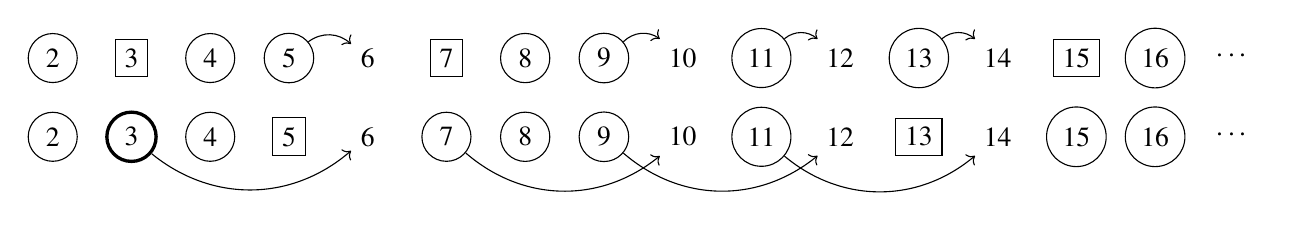
\begin{tikzpicture}
\fill node[circle,draw=black] (1-2) {2};
\fill node[draw, right of=1-2] (1-3) {3};
\fill node[circle,draw=black, right of=1-3] (1-4) {4};
\fill node[circle,draw=black, right of=1-4] (1-5) {5};
\fill node[right of=1-5] (1-6) {6};
\fill node[draw, right of=1-6] (1-7) {7};
\fill node[circle,draw=black, right of=1-7] (1-8) {8};
\fill node[circle,draw=black, right of=1-8] (1-9) {9};
\fill node[right of=1-9] (1-10) {10};
\fill node[circle,draw=black, right of=1-10] (1-11) {11};
\fill node[right of=1-11] (1-12) {12};
\fill node[circle,draw=black, right of=1-12] (1-13) {13};
\fill node[right of=1-13] (1-14) {14};
\fill node[draw, right of=1-14] (1-15) {15};
\fill node[circle,draw=black, right of=1-15] (1-16) {16};
\fill node[right of=1-16] {$\cdots$};

\draw[->, bend left=40] (1-5) to (1-6);
\draw[->, bend left=40] (1-9) to (1-10);
\draw[->, bend left=40] (1-11) to (1-12);
\draw[->, bend left=40] (1-13) to (1-14);

\fill node[circle,draw=black, below of=1-2] (2-2) {2};
\fill node[circle,draw=black, very thick, right of=2-2] (2-3) {3};
\fill node[circle,draw=black, right of=2-3] (2-4) {4};
\fill node[draw, right of=2-4] (2-5) {5};
\fill node[right of=2-5] (2-6) {6};
\fill node[circle,draw=black, right of=2-6] (2-7) {7};
\fill node[circle,draw=black, right of=2-7] (2-8) {8};
\fill node[circle,draw=black, right of=2-8] (2-9) {9};
\fill node[right of=2-9] (2-10) {10};
\fill node[circle,draw=black, right of=2-10] (2-11) {11};
\fill node[right of=2-11] (2-12) {12};
\fill node[draw, right of=2-12] (2-13) {13};
\fill node[right of=2-13] (2-14) {14};
\fill node[circle,draw=black, right of=2-14] (2-15) {15};
\fill node[circle,draw=black, right of=2-15] (2-16) {16};
\fill node[right of=2-16] {$\cdots$};

\draw[->, bend right=40] (2-3) to (2-6);
\draw[->, bend right=40] (2-7) to (2-10);
\draw[->, bend right=40] (2-9) to (2-12);
\draw[->, bend right=40] (2-11) to (2-14);
\end{tikzpicture}
\caption{Application of the three Lemmas in a small range.  Circles denote prohibitions of $\Sigma^2$--structures by \Cref{SigmaNonexistenceLemma}, arrows denote $\Sigma^2$--structures constructed by \Cref{SigmaArrowLemma}, and squares denote exceptional $\Sigma^2$--structures constructed by \Cref{SigmaSpecialCaseLemma}.}
\end{figure}

\begin{corollary}\label{LambdasAreFlat}
For $\G$ a formal group over $\Spec \F_2$ with $\height \G \le 2$, the maps $\lambda_2$ and $\lambda_3$ are flat.
\end{corollary}
\begin{proof}
This is a culmination of the above calculations.  As argued at the beginning of our algebraic analysis, it suffices to show just that $\lambda_2^\circ$ is faithfully flat to make the cocnclusion.  Flatness follows by showing that the map is surjective on tangent spaces, which is exactly the content of \Cref{SigmaNonexistenceLemma}, \Cref{SigmaArrowLemma}, and \Cref{SigmaSpecialCaseLemma}.
\end{proof}

\begin{theorem}\label{MStringTriumvirate}
Let $\G$ be a formal group over a perfect field of characteristic $2$, and assume $\height \G \le 2$.  For $E$ the associated Morava $K$--theory or $E$--theory, there are isomorphisms
\begin{align*}
\Spec E_0 M\String & \xrightarrow\cong \Sigma^3(\CP^\infty_E; \sheaf I(0)), &
\Spec E_0 M\Spin & \xrightarrow\cong C^2_{\mathrm{is}}(\CP^\infty_E; \sheaf I(0)),
\end{align*}
where $C^2_{\mathrm{is}}(\CP^\infty_E; \sheaf I(0))$ is the subscheme of $C^2(\CP^\infty_E; \sheaf I(0))$ consisting of those \index{inverse symmetric function}\textit{inverse-symmetric} functions satisfying $f(x, y) / f(-_{\G} x, -_{\G} y) = 1$.  The $E_0$--points of these schemes biject with ring spectrum maps $M\String \to E$ and $M\Spin \to E$ respectively.\footnote{This is sufficient to conclude the existence of the Atiyah--Bott--Shapiro orientation in the homotopy category.} \qed
\end{theorem}
\begin{proof}
Our goal all along was to use the algebraic model to govern the bar spectral sequences 
\begin{align*}
\Tor^{E_* \Spin/SU}_{*, *}(E_*, E_* BSU) & \Rightarrow E_* B\Spin, &
\Tor^{E_* \Spin/SU}_{*, *}(E_*, E_* BU[6, \infty)) & \Rightarrow E_* B\String. \\
\intertext{Our conclusion from \Cref{LambdasAreFlat} is that they are both concentrated on the $0$--line and isomorphic to the respective Hopf algebra quotients}
E_0 BSU \mmod (E_0 \Spin/SU) & \cong E_0 B\Spin, &
E_0 BU[6, \infty) \mmod (E_0 \Spin/SU) & \cong E_0 B\String.
\end{align*}
Our algebraic models furthermore explicitly identify these quotients on homological schemes as those subschemes on which the stated algebraic identities hold.  The final claim of the theorem follows from even-ness and the universal coefficient spectral sequence.
\end{proof}

\begin{corollary}\label{EllipticSpectraAreOrientedByString}
If $E$ is a finite height Morava $K$-- or $E$--theory considered as an elliptic spectrum, the complex $\sigma$--orientation of \Cref{EllipticSpectraAreOriented} lifts uniquely to a ring map $M\String \to E$.
\end{corollary}
\begin{proof}
An \emph{immediate} consequence of the canonical cubical structure associated to an abelian variety is that it automatically satisfies the extra condition required to be a $\Sigma^3$--structure.
\end{proof}

\begin{remark}[{\cite[Theorem 7.2]{HopkinsICMZurich}}]
More generally, the $\sigma$--orientation associated to a elliptic spectrum which either has $1/2 \in \pi_0 E$ or which has $\pi_* E$ torsion--free is supposed to lift through $M\String$.  Flatness in this setting is supposed to be approached via a fiber-by-fiber criterion, but here the grading tricked used above are less visibly helpful in lifting the classical algebraic result to the periodic one we require to make this work.  Rather than pursue this, we will give a sketch of the construction of the $\String$--orientation of $\tmf$ in \Cref{JuvitopTalkSection}, which automatically gives this much stronger result.
\end{remark}

\begin{remark}[{\cite{KLW,StricklandFSKS}}]
A the cohomology formal schemes of a number of other infinite loopspaces related to real $K$--theory admit reasonable descriptions, often even independent of height.  A routinely useful result in this arena is due to Yagita~\cite[Lemma 2.1]{Yagita}: for $k_\Gamma$ the connective cover of the Morava $K$--theory $K_\Gamma$, in the Atiyah--Hirzebruch spectral sequence \[E_2^{*, *} = Hk^* X \otimes_k k_\Gamma^* \Rightarrow k_\Gamma^* X,\] the differentials are given by \[d_r(x) = \begin{cases} 0 & \text{if $r \le 2(p^d - 1)$}, \\ \lambda Q_d x \otimes v_d & \text{if $r = 2(p^d - 1) + 1$} \end{cases}\] where $\lambda \ne 0$ and $Q_d$ is the $d${\th} Milnor primitive.  For instance, this shows that $K_* BO$ decomposes as \[K_* BO \cong K_*[b_2, b_4, b_{2^{d+1}-2}] \underset{K_*[b_{2j}^2 \mid j < 2^d]}{\otimes} K_*[b_{2j}^2].\]  This, coupled to a theorem governing the result of the double bar spectral sequence, powers most of the results of Kitchloo, Laures, and Wilson~\cite[Section 4]{KLW}.  Their stronger results on the connective covers of $BO \times \Z$ are summarized in \Cref{MoravaKthyOfBO}.  The remaining formal scheme $B\String_K$, our prized object, is harder to access by these means: the sequence $(\OS{HS^1}{2})_K \to B\String_K \to B\Spin_K$ is exact in the middle, but neither left- nor right-exact~\cite[pg.\ 234]{KLW}, causing significant headache.  Satisfyingly, their methods also tell us that our analysis fails at higher heights: the formal scheme $\Spin/SU_K$ contains $\coprod_{j \ge 3} (\OS{HS^1[2]}{j})_K$ as a subscheme, and it accounts for the kernel of the map to $B\Spin_K$.  Once $\height \Gamma \ge 3$ is satisfied, this kernel is nonzero.
\end{remark}

\begin{figure}
\begin{center}
\begin{tikzcd}
& \Div_0 \overline \Gamma[2] \arrow{rr} \arrow{ld} \arrow[equal]{dd} & & \Div_0 \overline \Gamma \arrow{ld} \arrow[equal]{dd} \\
\ker \omega \arrow[crossing over]{rr} \arrow{dd} & & B\Spin_K \\
& \Div_0 \overline \Gamma[2] \arrow{rr} \arrow{ld} \arrow[equal]{dd} & & \Div_0 \overline \Gamma \arrow{ld} \arrow[equal]{dd} \\
\SDiv_0 \Gamma[2] \arrow[crossing over]{rr} \arrow{dd} & & BSO_K \arrow[crossing over, "\omega" near end]{rr} \arrow[crossing over, leftarrow]{uu} & & \Gamma[2]^{\sm 2} \\
& \Div_0 \overline \Gamma[2] \arrow{rr} \arrow{ld} \arrow{dd} & & \Div_0 \overline \Gamma \arrow{ld} \arrow{dd} \\
\Div_0 \Gamma[2] \arrow[crossing over]{rr} \arrow{dd} & & BO_K \arrow[crossing over, "\sigma" near end]{rr} \arrow[crossing over, leftarrow]{uu} & & \Gamma[2] \\
& \Div \overline \Gamma[2] \arrow{rr} \arrow{ld} & & \Div \overline{\Gamma} \arrow{ld} \\
\Div \Gamma[2] \arrow{rr} & & (BO \times \Z)_K \arrow{rr} \arrow[leftarrow, crossing over]{uu} & & \underline{\Z}.
\end{tikzcd}
\end{center}
\caption{Presentations of the Morava $K$--theoretic cohomological formal schemes associated to connective covers of $BO \times \Z$.  Each level in the prism is a bi-Cartesian square in the category of formal group schemes, and each level is the fiber of the maps off of the previous level to the Postnikov section.  The formal curve $\overline \Gamma$ is $\HP^\infty_K$, which is the fiber of $\sigma\co \Div_2^+ \Gamma \to \Gamma$, and $\overline \Gamma[2]$ is the fiber of the lift of the endo-isogeny $2\co \Gamma \to \Gamma$ to $\overline \Gamma$.  The map $\sigma$ vanishes on $\Div_0 \overline \Gamma$ and acts by summation on $\Div_0 \Gamma[2]$.  The map $\omega$ vanishes on $\Div_0 \overline \Gamma$ and acts on $\SDiv_0 \Gamma[2] \cong C_2 \Gamma[2]$ by $[a, b] \mapsto a \wedge b$.}\label{MoravaKthyOfBO}
\end{figure}

\begin{remark}
There are variations on this analysis that remain to be sorted out.  For instance, there is a naturally occurring orientation $MU \to MSO$, whose associated genus factors through the quotient of the Lazard ring by the relation $[-1](x) = -x$.  This factored map is injective and it becomes an isomorphism after inverting $2$---but, without inverting $2$, $MSO_*$ itself is populated by plenty of $2$--torsion.  It would be nice to have available an interpretation of such real orientations in terms of formal group laws.
\end{remark}










\todo{Mention all this work of Gerd.  He has a bunch of papers that are all clustered around these topics.}













\appendix

% -*- root: main.tex -*-



\chapter{Power Operations}\label{PowerOpnsChapter}

\begin{center}
\textbf{Convention: We will write \(E\) for \(E_\Gamma\), \(\Gamma\) a fixed formal group of finite height, for the entirety of this Appendix.}
\end{center}

Our goal in this Appendix is to give a tour of the interaction of the \(\sigma\)--orientation with a topic of modern research, the theory of \index{E infty ring spectrum@\(E_\infty\)--ring spectrum}\(E_\infty\)--ring spectra, in a manner consistent with the rest of the topics in this book.  Because the theory of \(E_\infty\)--ring spectra (in particular: their algebraic geometry) is still very much developing, we have no hope of stating results in their maximum strength or giving a completely clear picture---as of this writing, the maximum strength is unknown and the picture is still resolving.  Although \(E_\infty\)--ring spectra themselves were introduced decades ago, we will even avoid giving a proper definition of them here, instead referring to the original work of May and collaborators~\cite{EKMM} and the more recent work of Lurie~\cite[Chapter 7]{LurieHA} for a proper treatment.  In acknowledgement of this underwhelming level of rigor, we have downgraded our discussion from a Case Study to an Appendix.\footnote{Additionally, the contents of this Appendix did not make it into the classroom version of this course, though the latter two sections did appear as contributed talks to graduate student seminars.}

As far as we are concerned, \(E_\infty\)--ring spectra arise in order to solve the following problem: given two ring spectra \(R\) and \(S\) in the homotopy category, the set of homotopy classes of ring maps \(\CatOf{RingSpectra}(R, S)\) forms a subset of the set of all homotopy classes \([R, S] = \pi_0 \CatOf{Spectra}(R, S)\), selected by a homomorphism condition.  There is no meaningful way to enrich this to a \emph{space} of ring spectrum maps from \(R\) to \(S\), which inhibits us from understanding an obstruction theory for ring spectra, i.e., approximating \(R\) by ``nearby'' ring spectra \(R'\) in a way that relates \(\CatOf{RingSpectra}(R, S)\) and \(\CatOf{RingSpectra}(R', S)\) by a fiber sequence.\index{obstruction theory}

The extra data that accomplishes this mapping space feat turns out to be an explicit naming of the homotopies controlling the associativity and commutativity of the ring spectrum multiplication, which are subject to highly intricate compatibility conditions.\footnote{This is rather analogous to the extra data required on a \emph{space}, beyond just a multiplication, which allows one to use the bar construction to assemble a delooping.}\footnote{The high degree of intricacy accomplishes this goal of constructing mapping spaces, but it interacts strangely with the classical notion of a ring spectrum in the homotopy category: there are ring spectrum maps that admit \emph{no} enrichment to an \(E_\infty\) map, and there are ring spectrum maps that admit \emph{multiple} enrichments to \(E_\infty\) maps.}  Again, rather than spell this out, it suffices for our purposes to say that there is such a notion of a structured ring spectrum that begets a mapping space between two such.  We also record the following conglomerate theorem as indication that this program overlaps with the one we have been describing already:
\begin{theorem}\label{OmnibusEinftyTheorem}
The following are examples of \(E_\infty\)--ring spectra:
\begin{itemize}
    \item (\cite[Section VIII.1]{MayRingSpacesSpectra}) The classical \(K\)--theories \(KU\) and \(KO\).
    \item (\cite[Section VIII.1]{MayRingSpacesSpectra}) The Eilenberg--Mac Lane spectra \(HR\).
    \item (\cite[Corollary 7.6--7]{GoerssHopkins}) The Morava \(E\)--theories \(E_\Gamma\) and their fixed point spectra.\footnote{Notably, the Morava \(K\)--theories are \emph{not} \(E_\infty\)--rings at finite heights, in view of \Cref{HinftyRingsModp}.}
    \item (\cite[Section IV.3]{MayRingSpacesSpectra}) The Thom spectra arising from the \(J\)--homomorphism, including \(MO\), \(M\SO\), \(M\Spin\), \(M\String\), \(MU\), \(M\SU\), and \(MU[6, \infty)\).
    \item (\cite{BehrensConstruction}, cf.\ \Cref{ConstructionOfTMFSection}) The spectra \(\TMF\), \(\Tmf\), and \(\tmf\). \qed
\end{itemize}
\end{theorem}

The forgetful map from \(E_\infty\)--rings down to ring spectra in the homotopy category factors through an intermediate category, that of \(H_\infty\)--ring spectra, which captures the extra factorizations expressing these associativity and commutativity relations.  Specifically, recall the following definition from the discussion in \Cref{QuillenPowerOpnsSection}:

\begin{definition}[{\cite[Definition I.3.1]{BMMS}, cf.\ \Cref{QuillenPowerOpnsSection}}]
An \index{H infty ring spectrum@\(H_\infty\)--ring spectrum}\(H_\infty\)--ring spectrum is a ring spectrum \(E\) equipped with factorizations \(\mu_n\) as in
\begin{center}
\begin{tikzcd}
E^{\sm n} \arrow["\mu"]{r} \arrow{d} & E \\
E^{\sm n}_{h\Sigma_n} \arrow{ru}[description]{\mu_n},
\end{tikzcd}
\end{center}
which are subject to compatibilities induced by the inclusions \(\Sigma_n \times \Sigma_m \subseteq \Sigma_{n+m}\) and the inclusions \(\Sigma_n \wr \Sigma_m \subseteq \Sigma_{nm}\).
\end{definition}

\begin{lemma}
Each \(E_\infty\)--ring spectrum gives rise to an \(H_\infty\)--ring spectrum in the homotopy category. \qed
\end{lemma}

\noindent We care about this secondary definition because our results thus far have all concerned the cohomology of spaces, which is, at its core, a calculation at the level of \emph{homotopy classes}.  This is therefore as much of the \(E_\infty\)--structure as one could hope would interact with our analyses in the preceding Case Studies.

In \Cref{QuillenPowerOpnsSection} we introduced an \(H_\infty\)--ring structure on \(MU\), and in \Cref{StabilizingTheMUSteenrodOps} and \Cref{CalculationOfMUStarSection} we used it to make a calculation of the coefficient ring \(MU_*\).  Our first goal in this Appendix is to introduce an \(H_\infty\)--ring structure on certain chromatically interesting spectra, including Morava's theories \(E_\Gamma\), and to describe the compatibility laws arising from intertwining these two \(H_\infty\)--structures.  The culminating result is as follows:

\begin{theorem}[{cf.\ \Cref{AHSHinftyResultForEthy}}]
An orientation \(MU[6, \infty) \to E_\Gamma\) is \(H_\infty\) if and only if the induced cubical structure is \index{norm!coherence}``norm-coherent'' (cf.\ \Cref{NormCoherentDefn}). \qed
\end{theorem}

\noindent Before addressing this, we discuss in \Cref{CharacterTheorySection} an important phenomenon: after deleting certain forms of torsion, the Morava \(E_\Gamma\)--homology of a finite spectrum can be well--approximated by its Morava \(E_{\Gamma'}\)--homology where \(\Gamma'\) satisfies \(\height{\Gamma'} < \height{\Gamma}\).  This is interesting in its own right, and we will see that the approximation bears directly on the study of power operations.

Secondly, with the homotopy category exposed, we turn to \(E_\infty\)--ring spectra themselves: in \Cref{ConstructionOfTMFSection} we introduce the spectrum \(\TMF\), which is the primary target of the \(\String\)--orientation; and in \Cref{JuvitopTalkSection}, we indicate the construction of an \(E_\infty\) orientation of $\TMF$, providing full details in the simpler case of the construction of the \(\Spin\)--orientation of \(KO\).













\section{Rational chromatic phenomena (Nathaniel Stapleton)}\label{CharacterTheorySection}

Before embarking on the ambitious project of understanding the collection of \(H_\infty\)--ring maps \(\phi\co MU[6, \infty) \to E_\Gamma\), it would be instructive to be able to answer the following: if we had such an orientation, would data could we extract from it?  The main feature of such a map is that it belongs to a commutative diagram
\begin{center}
\begin{tikzcd}
MU[6, \infty)^0(X) \arrow["\phi"]{r} \arrow["P^{\Sigma_n}_{MU[6, \infty)}(X)"]{d} & E^0(X) \arrow["P^{\Sigma_n}_E(X)"]{d} \\
MU[6, \infty)^0(B\Sigma_n \times X) \arrow["P^{\Sigma_n}(\phi)"]{r} & E^0(B\Sigma_n \times X).
\end{tikzcd}
\end{center}
Before understanding the maps in this commutative diagram, we must understand its nodes.  There is a natural map \[E^0(B\Sigma_n) \otimes_{E^0} E^0(X) \to E^0(B\Sigma_n \times X),\] and whether it is an equivalence is highly dependent on the structure of \(E^0(B\Sigma_n)\) itself---for instance, this would be the case if \(E^0(B\Sigma_n)\) were flat as an \(E^0\)--module.  For this reason, we are strongly motivated to feel out any foothold on this object that we are able to find, and a critical such foothold is the chromatic character theory of Hopkins, Kuhn, and Ravenel~\cite{HKR}.  Their theorems describe the Morava \(E\)--cohomology of a finite group with certain forms of torsion (e.g., \(p\)--torsion) deleted, and we give an introduction to their results in this Lecture.\footnote{The intrepid reader who finds this material interesting should also look at: the paper by Morava~\cite{MoravaLocalFieldsExtraordinaryKthy}, which discusses much of the same material here in slightly different terms; the paper by Greenlees--Strickland~\cite{GreenleesStrickland}, which discuss a ``transchromatic'' version of these results, where they study the object $i_d^* j_d{}_* (\moduli{fg})^\wedge_\Gamma$ of \Cref{LEFTRealTheoremWithProof}; and the paper by Stapleton~\cite{Stapleton}, which streamlines and generalizes the results of Greenlees--Strickland by invoking the geometry of $p$--divisible groups.}



% -*- root: main.tex -*-

\subsection*{The \(E_{\Gamma}\)-cohomology of finite abelian groups}

%Ask Eric to change 3.5.2 to have an arbitrary k.

%Introduce \(E = E_{\Gamma}\), the universal deformation, and borel equivariant cohomology theories. Use 2.6.1 to identify \(E^*(BC_p)\) (look at how gradings have been discussed in the book ie. graded formal schemes?). Use Kunneth to identify \(E^*(BA)\). End by introducing the ``approximation problem", approximating \(E^0(X)\) be rational cohomology - good for finite complexes, bad for big complexes.

Let \(\Gamma\) be a height \(d\) formal group over \(k\), a perfect field of characteristic \(p\). By \Cref{LubinTateModuliThm}, there is a noncanonical isomorphism 
\[
\sheaf O_{(\moduli{fg})^\wedge_\Gamma} \cong W(k)\ps{u_1, \ldots, u_{d-1}}
\] 
and this ring carries the universal deformation of \(\Gamma\), which we denote as \(\G\). By \Cref{DefnChromaticHomologyThys}, there is an associated chromatic cohomology theory
\[
E = E_{\Gamma}
\]
called height \(d\) Lubin--Tate theory or Morava \(E\)--theory such that
\[
\CP^\infty_E = BS^1_E = \Spf(E^0(BS^1)) = \G.
\]
Fixing a coordinate on \(\G\) provides us with a formal group law
\[
x +_{\G} y.
\]

\begin{proposition}[{\cite[Proposition 5.2 and Lemma 5.7]{HKR}, cf.\ \Cref{KtheoryOfClassifyingSpace}}] \label{app:cyclic}
Let \(C_{m} = S^1[m]\). There is an isomorphism (depending on the chosen coordinate) 
\[
E^*(BC_{m}) \cong E^*\ps{x}/([m]_{\G}(x))
\]
of \(E^*\)-algebras. Moreover, \(E^*(BC_{m})\) is free as an \(E^*\)-module of rank \(p^{kd}\) where \(p^k|m\) and \(p^{k+1} \nmid m\).\footnote{To prove this result it is most natural to set \(|x| = 2\), but for the purposes of this Lecture (and, indeed, this textbook) it is most natural to set \(|x| = 0\). We can move back and forth between these choices by the change of coordinates \(x \leftrightarrow ux\), where \(u\) is a generator of \(\pi_2 E\).} \pushQED\qed \qedhere \popQED
\end{proposition}

\begin{corollary}[{\cite[Corollary 5.10]{HKR}}] \label{app:ab}
Let 
\[
A \cong C_{m_1} \times \cdots \times C_{m_i}
\]
be a finite abelian group.  There is then an isomorphism of \(E^*\)-algebras
\[
E^*(BA) \cong E^*\ps{x_1, \ldots, x_{i}}/([m_1]_{\G}(x_1), \ldots, [m_i]_{\G}(x_i)). \pushQED\qed \qedhere \popQED
\]
\end{corollary}


If \(A \cong C_{p^{k_1}} \times \cdots \times C_{p^{k_i}}\) is an abelian \(p\)-group, it follows that \(E^*(BA)\) is a free \(E^*\)-module of rank \(p^{k_1d+\cdots + k_id}\). If \(m\) is prime to \(p\), then \([m]_{\G}(x)/x\) is a unit in \(E^*\ps{x}\). This implies that the rank of \(E^*(BA)\) only depends on the Sylow \(p\)-subgroup of \(A\). Even more, it implies that the inclusion of the Sylow \(p\)-subgroup of \(A\) into \(A\) induces an isomorphism after applying $E$-cohomology. We will now always assume that \(A\) is an abelian \(p\)-group.

The most computable of chromatic cohomology theories is periodic rational cohomology. For a \(\Q\)-algebra \(R\), the formal group associated to \(HRP\) is the (height \(0\)) additive formal group. It is natural to want to gain information regarding \(E^*(X)\) (for any chromatic cohomology theory \(E\)) by comparing \(E\)-cohomology with periodic rational cohomology.\footnote{We have employed a similar-sounding strategy elsewhere in this text, where we have approximated an arbitrary complex-orientable theory by \(\HFp P\), using the fact that the infinite-height group \(\G_a \otimes \F_p\) is a dense point in \(\moduli{fg} \times \Spec \Z_{(p)}\).  However, the height \(0\) point \(\G_a \otimes \Q\) is \emph{not} dense, and so our intention here is much more delicate.}  For instance, this is the purpose of the classical Chern character: for \(X\) a space, the Chern character is a map of commutative rings
\[
KU^0(X) \to H\Q P^0(X)
\] 
induced by the map of spectra\footnote{We could replace \(\Q\) with \(\R\) or \(\C\) and the result would still hold.} \[KU \to H\Q \wedge KU \simeq H\Q P.\] For \(X\) a finite \(CW\)-complex, it induces an isomorphism
\[
\Q \otimes KU^0(X) \cong H\Q P^0(X).
\]

When \(X\) is a finite CW complex, there is an isomorphism
\begin{equation*}
\Q \otimes E^*(X) \cong H(\Q \otimes E^0)P^*(X).
\end{equation*}
This follows from the fact that \(\Q \otimes E^*\) is a flat \(E^*\)-algebra. When \(X\) is not a finite CW complex, Proposition \ref{app:ab} gives a non-example. It implies that
\[
\Q \otimes E^*(BA)
\]
is free as a \(\Q \otimes E^*\)-module of rank \(p^{k_1d + \ldots + k_id}\). However, \[H(\Q \otimes E^0)P^*(BA) \cong \Q \otimes E^*\] is free of rank \(1\), a direct consequence of Maschke's theorem.

To explain one of the inputs into the main theorem of this Lecture, we need one more notion. For \(G\) a finite group, a \(G\)--CW complex \(X\) is a \(G\)--space built inductively by attaching ``cells'' of the form \((G/H) \times D^n\), as in the following pushout diagram:
\begin{center}
\begin{tikzcd}
\coprod_{i \in I} (G/H_i \times S^{n-1}) \arrow{r} \arrow{d} & \coprod_{i \in I} (G/H_i \times D^n) \arrow{d} \\
X^{(n-1)} \arrow{r} & X^{(n)}.
\end{tikzcd}
\end{center}
We say that a \(G\)--CW complex is finite if it can be built out of finitely many cells of the form \(G/H \times D^n\).

\begin{theorem}[{Equivariant CW Approximation, \cite[Theorem I.3.6]{MayAlaskaNotes}}] \label{app:CWapprox}
Every \(G\)--space is weakly equivalent to a \(G\)--CW complex. \qed
\end{theorem}

Given a cohomology theory \(E\), an equivariant version of the cohomology theory can be formed by setting
\[
E^{*}_{G}(X) = E^*(X_{hG}),
\]
where \(X\) is a \(G\)-space and
\[
X_{hG} \simeq EG \times_G X = (EG \times X)/G
\]
is the homotopy orbits for the \(G\)-action on \(X\). The resulting equivariant cohomology theory is called \textit{Borel equivariant \(E\)--theory}.

The purpose of this Case Study is to explain, in the case of \(E = E_{\Gamma}\), how to extend the above formula \[\Q \otimes E^*(X) \cong H(\Q \otimes E^0)P^*(X),\] originally stated for finite complexes \(X\), to an analogous formula for finite \(G\)--CW complexes. Said another way, for each finite group, we want to approximate Borel equivariant \(E\)--cohomology (restricted to finite \(G\)--CW complexes) by some version of Borel equivariant rational cohomology. We call this ``the approximation problem".  In particular, this encompasses our original goal of understanding \(E^*(B\Sigma_n)\), as it appears as a special case of Borel equivariant cohomology as in the formula \[E^*(B\Sigma_n) = E_{\Sigma_n}^*((\Sigma_n / \Sigma_n) \times *).\]

\subsection*{Formal Geometry}

%p-divisible groups from formal groups (reference 4.4-5.1). Algebro-geometric description of \(\Spf E^0(BA)\). Fix \(S^1\), build p-divisible group from \(p^k\)-torsion in \(S^1\). Note that all of this makes sense over \(\Spec E^0\). Return to approximation problem for \(E^0(BC_{p^k})\), phrase it in an algebro geometric way and work out the need to build \(C_0\).

Recall from \Cref{DefnPDivGp} that associated to a finite height formal group is a connected \(p\)--divisible group built out of the \(p^k\)--torsion of the formal group as \(k\) varies. Associated to the universal deformation \(\G\) is the following \(p\)--divisible group of height \(d\)
\[
\G[p] \hookrightarrow \G[p^2] \hookrightarrow \ldots,
\]
where the maps are the inclusions of the \(p^k\)--torsion into the \(p^{k+1}\)--torsion.  \Cref{app:cyclic} implies first 
\[
B(C_{p^k})_{E} \cong \G[p^k],
\]
and that the \(p\)--divisible group associated to \(\G\) can be formed using the inclusions \(C_{p^k} = S^1[p^k] \hookrightarrow C_{p^{k+1}} = S^1[p^{k+1}]\). 
%as the system of schemes
%\[
%BS^1[p]_{E} \hookrightarrow BS^1[p^2]_{E} \hookrightarrow \ldots.
%\]
\Cref{app:cyclic} also implies that all of the schemes in this system are finite flat commutative group schemes over \(\Spf E^0\). The \(p\)--divisible group is called ``height \(d\)'' because \(\G[p]\) is a finite group scheme of order \(p^d\) or, equivalently, since \(E^0(BC_p)\) has rank \(p^d\) as a free module over \(E^0\).

There are \(p\)--divisible groups that are \emph{not} built from formal groups, and the simplest of these plays a role in this story.  We define the \textit{constant \(p\)--divisible group of height \(1\)} to be 
\[
C_{p^{\infty}} = S^1[p^\infty] = \colim \big ( C_p \hookrightarrow C_{p^2} \hookrightarrow \ldots \big ).
\]
It is called \textit{constant} because it is made up of constant group schemes, and it is called height \(1\) because \(|S^1[p]| = p^1\).  The constant \(p\)--divisible group of height \(d\) is then the \(d\)--fold product \(C_{p^\infty}^{\times d} = (S^1)^{\times d}[p^\infty]\). The constant height \(d\) \(p\)-divisible group \(C_{p^\infty}^{\times d}\) is the unique height \(d\) \(p\)-divisible group $\G[p^{\infty}]$ with the property that
\[
\sheaf O_{\G[p^k]} \cong \prod_{C_{p^k}^{\times d}}R,
\]
where $R$ is the base ring.\footnote{An unimportant aside: a generic \(p\)--divisible group contains a maximal formal subgroup, and the quotient by this subgroup is an \textit{\'etale group}---and, whatever these are, they (and the attendant extension problems) form the ``new'' components of the theory of \(p\)--divisible groups.  In the case of a ground field of positive characteristic, \'etale groups admit a pleasant characterization: they are exactly those that become isomorphic to the constant group after base-change to the algebraic closure, and so in this sense the constant \(p\)--divisible groups of different ranks play a role similar to the Honda formal group laws of \Cref{FGpsOverAlgClosedFields}.}

%Let \(R\) be a commutative ring. There is a functor from finite abelian groups to finite commutative group schemes over \(\Spec(R)\) sending \(A\) to \(\Spec(\prod_{A}R)\). The constant height \(d\) \(p\)-divisible group \(C_{p^\infty}^{\times d}\) is the unique height \(d\) \(p\)-divisible group with the property that its \(p^k\)-torsion is in the image of this functor for all \(k\).

More generally, a similar description of \(BA_{E}\) can be given using formal geometry when \(A\) is a finite abelian group. Let \(A^*\) be the Pontryagin dual of \(A\) and let
\[
\InternalHom{FormalGroups}(A^*, \G)
\]
be the formal scheme that associates to a complete local \(E^0\)--algebra \(R\)
\[
\InternalHom{FormalGroups}(A^*, \G)(R) = \CatOf{AbelianGroups}(A^*, \G(R)).
\]
For large enough \(k\), we have \(A = A[p^k]\), and from this it follows that any map from \(A^*\) to \(\G(R)\) must land in the \(p^k\)--torsion \(\G[p^k](R)\).  There is thus an isomorphism of formal schemes
\[
\InternalHom{FormalGroups}(A^*, \G) \cong \InternalHom{FormalGroups}(A^*, \G[p^k]).
\]
\begin{proposition}[{\cite[Proposition 5.12]{HKR}}] \label{app:abeliangroupdualhom}
There is a canonical isomorphism of formal schemes
\[
\Spf(E^0(BA)) \cong \InternalHom{FormalGroups}(A^*, \G),
\]
natural in maps of finite abelian groups. \qed
\end{proposition}


The formal scheme \(\InternalHom{FormalGroups}(A^*,\G)\) is finite and flat over \(\Spf(E^0)\). Because of this, this formal scheme can be viewed as a scheme---really a scheme, and not a formal scheme!---over \(\Spec(E^0)\). Without going into the technical details of formal to informal constructions, the main idea is that the topology on a complete local \(E^0\)-algebra is not important to \(\G[p^k]\): for a continuous \(E^0\)-algebra \(R\), there is a bijection
\[
\CatOf{Algebras}_{E^0}^{\mathrm{cts}}(E^0(BC_p),R) \cong \CatOf{Algebras}_{E^0}(E^0(BC_p),R).
\]
The same cannot be said for \(E^0(BS^1)\).  In the case of our \emph{finite} abelian group $A$, we may thus restrict our attention to the scheme
\[
\InternalHom{FormalGroups}(A^*,\G[p^k]) \co \CatOf{Algebras}_{E^0} \rightarrow \CatOf{Sets}
\]
sending an \(E^0\)--algebra \(R\) to
\[
\CatOf{AbelianGroups}(A^*, \G[p^k](R)) \cong \CatOf{GroupSchemes}(A^*, \Spec(R) \underset{{\Spec(E^0)}}{\times} \G[p^k]).
\]
Since the ring map \(E^0 \rightarrow \Q \otimes E^0\) is not continuous, this discussion is important to phrasing an algebro-geometric version of the appoximation problem explained at the end of the previous section.

When \(G = A\) and \(X = *\), the approximation problem can now be given an algebro-geometric description: we would like to find a \((\Q \otimes E^0)\)--algebra \(R\) such that 
\[
\Spec(R) \times \InternalHom{FormalGroups}(A^*, \G[p^k]) \cong  \InternalHom{FormalGroups}(A^*, \Spec(R) \times \G[p^k])
\]
is recognizable as \(\Spec(-)\) of the \(HRP\)-cohomology of a space. This would only solve the approximation problem for \(E^0(BA)\)---but, astoundingly, it will turn out that this is enough.

There is a surprisingly simple answer to the approximation problem in this case.  Fix\footnote{This choice of \(\Lambda\) is the only choice made in this Lecture, and the last subsection of this Lecture addresses how natural the character map is in automorphisms of \(\Lambda\).  From a certain perspective, the results of Barthel--Stapleton~\cite{BarthelStapleton} can be viewed as an analysis of how natural the character map is among finite index maps \(\Lambda \hookrightarrow \Lambda\).} \(\Lambda = \Z_{p}^{d}\) and let \(\Lk = \Lambda/p^k\Lambda\), so that there are non-canonical isomorphisms
\[
\Lambda^* \cong (\Q/\Z_{(p)})^d \cong (S^1[p^{\infty}])^d
\] 
as well as canonical isomorphisms
\begin{align*}
\Lambda^* & \cong (S^1[p^{\infty}])^d, &
\Lambda^*[p^k] & \cong (\Lambda_{k})^* \cong \CatOf{Groups}(\Lambda_k, C_{p^k}).
\end{align*}
%Let \(\Lk = (C_{p^k}^{\times d})^*\) so that there are canonical isomorphisms
%\[
%\Lk^* \cong (S^1)^{\times d}[p^k] = C_{p^k}^{\times d}.
%\]
If we could find an \(R\), dependent on \(\G\), such that
\[
\Spec(R) \times_{\Spec(E^0)} \G[p^k] \cong \Lk^*
\]
as abelian group schemes, then we would be done, since
\[
\sheaf O_{\Lk^*} \cong \prod_{\Lk^*} R \cong HRP^0\left(\coprod_{\Lk^*} \ast\right)
\]
and
\begin{align*}
\Spec(R) \times_{\Spec(E^0)} \InternalHom{FormalGroups}(A^*, \G[p^k]) & \cong \InternalHom{FormalGroups}(A^*, \Lambda_{k}^*) \\
& \cong A^{\times d}.
\end{align*}
That is, we would be able to give the simplest answer imaginable: we will have approximated \(E^0(BA)\) by the \(HRP\)-cohomology of a collection of points. In the next section we construct a \(\Q \otimes E^0\)-algebra \(C_0\) with this property.


%Let \(\Lk = (\Z/p^k)^n\) so that there are canonical isomorphisms
%\[
%\Lk^* \cong (\Z^n)^*[p^k] \cong (S^1)^n[p^k] \cong (C_{p^k})^n.
%\]
%If we could find an \(R\) such that
%\[
%\Spec(R) \times_{\Spec(E^0)} \G[p^k] \cong \Lk^*
%\]
%as abelian group schemes, then we would win since
%\[
%\sheaf O_{\Lk^*} \cong \prod{\Lk^*} R \cong HR^*(\coprod{\Lk^*} \ast)
%\]
%and
%\[
%\Spec(R) \times_{\Spec(E^0)} \Hom(A^*, \G[p^k]) \cong \Hom(A^*, (C_{p^k})^n) \cong A^n.
%\]
%That is, we would be able to give the simplest answer imaginable - we will have approximated \(E^0(BA)\) by the \(HRP\)-cohomology of a collection of points. The purpose of the next section is to construct a \(\Q \otimes E^0\)-algebra \(C_0\) with this property.


\subsection*{The ring \(C_0\)}
%Essentially follow the construction in the current document.


The goal of this section is to construct a \((\Q \otimes E^0)\)--algebra \(C_0\) such that
\[
\Spec(C_0) \times_{\Spec(E^0)} \G[p^k] \cong \Lambda_{k}^*
\]
for each \(k>0\). That is, there should be an isomorphism of \(p\)--divisible groups
\[
\Spec(C_0) \times_{\Spec(E^0)} \G[p^\infty] \cong \Lambda^*.
\]
This does not uniquely specify \(C_0\), but we can fix this deficiency by asking that \(C_0\) carry the universal isomorphism of \(p\)-divisible groups 
\[
u \co \Lambda^* \xrightarrow{\cong} \Spec(C_0) \times_{\Spec(E^0)} \G[p^\infty].
\]
This means that, given any \(E^0\)--algebra \(T\) and an isomorphism of \(p\)--divisible groups
\[
f \co \Lambda^* \xrightarrow{\cong} \Spec(T) \times_{\Spec(E^0)} \G[p^\infty],
\]
there is a unique map of \(E^0\)--algebras
\[
C_0 \xrightarrow{u_f} T
\]
such that \(f = \Spec(T) \times_{\Spec(C_0)} u\), where the pullback is along \(u_f\).

The idea of the construction of \(C_0\) is quite simple.  \Cref{app:abeliangroupdualhom} implies \[E^0(B\Lk) \cong \sheaf O(\InternalHom{FormalGroups}(\Lk^*,\G[p^k])).\]  To construct \(C_0\), it suffices to understand the open subscheme of the mapping scheme \(\InternalHom{FormalGroups}(\Lk^*,\G[p^k])\) which consists of the homomorphisms that are isomorphisms. 

Since \(E^0(B\Lk)\) corepresents \(\InternalHom{FormalGroups}(\Lk^*,\G[p^k])\), it carries the universal homomorphism of group schemes
\[
u \co \Lk^* \rightarrow \G[p^k].
\]
Thus the identity map \(E^0(B\Lk) \xrightarrow{1} E^0(B\Lk)\) corresponds to a homomorphism of abelian groups
\[
\Lk^* \rightarrow \G[p^k](E^0(B\Lk))
\]
or equivalently a map of commutative group schemes
\[
u \colon \Lk^* \rightarrow \Spec(E^0(B\Lk)) \times_{\Spec(E^0)} \G[p^k].
\]
This map is a consequence of the exponential adjunction for finite flat commutative group schemes: the identity map
\[
1 \co \InternalHom{FormalGroups}(\Lk^*,\G[p^k]) \to \InternalHom{FormalGroups}(\Lk^*,\G[p^k])
\]
is adjoint to the evaluation map
\[
\mathrm{ev} \co \Lk^* \times  \InternalHom{FormalGroups}(\Lk^*,\G[p^k]) \to \G[p^k].
\]
Given \(\alpha \in \Lk^*\), the naturality of Proposition \ref{app:abeliangroupdualhom} implies that the behavior of
\[
\InternalHom{FormalGroups}(\Lk^*,\G[p^k]) \to \G[p^k]
\]
on rings of functions is precisely
\[
E^0(B\alpha) \co E^0(BC_{p^k}) \to E^0(B\Lk).
\]
Using the fixed coordinate \(x\), this is equivalent to a map of \(E^0(B\Lk)\)-algebras
\[
u^* \co E^0(B\Lk)\ps{x}/[p^k]_{\G}(x) \xrightarrow{} \prod_{\Lk^*} E^0(B\Lk).
\]
Fixing a set of generators for \(\Lk^*\), gives an isomorphism
\[
E^0(B\Lk) \cong E^0\ps{x_1, \ldots, x_d}/([p^k]_{\G}(x_1), \ldots, [p^k]_{\G}(x_d)),
\]
and the behavior of \(u^*\) on the factor corresponding to \((i_1, \ldots, i_d) \in \Lk^*\) is then
\[
u^* \colon x \mapsto [i_1]_{\G}(x_1)+_{\G} \ldots +_{\G} [i_k]_{\G}(x_d).
\]
By \Cref{app:ab}, these are free \(E^0(B\Lk)\)-modules of the same rank. To force the map to be an isomorphism, it suffices to invert the determinant. Let
\begin{align*}
S_k &= \im \big (\Lk^* \setminus 0 \rightarrow \G[p^k](E^0(B\Lk)) \big ) \\ &= \{ [i_1]_{\G}(x_1)+_{\G} \ldots +_{\G} [i_d]_{\G}(x_d)| 0 \neq (i_1, \ldots, i_d) \in \Lk^* \}.
\end{align*}

\begin{lemma} \label{det}
Inverting the determinant of \(u^*\) is equivalent to inverting \(S_k\).
\end{lemma}
\begin{proof}
For \(\bar{i} = (i_1, \ldots, i_d) \in \Lk^*\), set
\[
[\bar{i}](\bar{x}) = [i_1]_{\G}(x_1) +_{\G} \ldots +_{\G} [i_d]_{\G}(x_d).
\]
The matrix defining \(u^*\) is given by the Vandermonde matrix
\[
\left(
\begin{array}{ccccc}
1 & [\bar{j_1}](\bar{x}) & [\bar{j_1}](\bar{x})^2 & \ldots & [\bar{j_{1}}](\bar{x})^{p^k-1} \\
1 & [\bar{j_2}](\bar{x}) & [\bar{j_2}](\bar{x})^2 & \ldots & [\bar{j_{2}}](\bar{x})^{p^k-1}\\
\vdots & \vdots & \vdots & \ddots & \vdots \\
1 & [\bar{j_{p^k}}](\bar{x}) & [\bar{j_{p^k}}](\bar{x})^2 & \ldots & [\bar{j_{p^k}}](\bar{x})^{p^k-1}\\
\end{array} \right),
\]
where \(\{\bar{j_1},\ldots,\bar{j_{p^k}}\} = \Lk^*\).
The determinant of this matrix is
\[
\prod_{1 \leq s < t \leq p^k} ([\bar{j_t}](\bar{x}) - [\bar{j_s}](\bar{x})).
\]
It is a basic fact of subtraction for formal group laws that
\[
x -_{\G} y = v(x-y)
\]
for a unit \(v\). 
Thus the determinant is, up to multiplication by a unit, 
\begin{align*}
\prod_{1 \leq s < t \leq p^k} ([\bar{j_t}](\bar{x}) -_{\G} [\bar{j_s}](\bar{x})) & = \prod_{1 \leq s < t \leq p^k} ([\bar{j_t} - \bar{j_s}](\bar{x})) \\
& = \prod_{0 \neq \bar{j} \in \Lk^*} [\bar{j}](\bar{x})^{p^k-1}. \qedhere
\end{align*} 
\end{proof}

\begin{corollary}
Inverting \(S_k\) in \(E^0(B\Lk)\) inverts \(p\). \pushQED\qed \qedhere \popQED
\end{corollary}

Set \(C_{0,k} = S_{k}^{-1}E^0(B\Lk)\).  The set \(S_k\) consists largely of zero divisors. Because of this, we should be concerned that \(C_{0,k}\) is the zero ring. The following result of Hopkins--Kuhn--Ravenel saves the day:

\begin{proposition}[{\cite[Proposition 6.5]{HKR}}]\label{CZeroIsFaithfullyFlat}
The ring \(C_{0,k}\) is a faithfully flat \(\Q \otimes E^0\)-algebra. \pushQED\qed \qedhere \popQED
\end{proposition}

By construction, the \(E^0\)--algebra \(C_{0,k}\) carries the universal isomorphism
\[
\Lk^* \xrightarrow{\cong} \G[p^k].
\]
It follows that the colimit \[C_0 = \colim_{k} C_{0,k}\] carries the universal isomorphism of \(p\)--divisible groups
\[
\Lambda^* \xrightarrow{\cong} C_0 \otimes \G.
\]
This is because a map \(C_0 \rightarrow R\) is a compatible system of maps \(C_{0,k} \rightarrow R\) and the map \(C_{0,k} \rightarrow C_{0,k+1}\) restricts the universal isomorphism
\[
\Lambda_{k+1}^{*} \xrightarrow{\cong} \G[p^{k+1}]
\]
to the \(p^k\)--torsion.
%
%
% \(C_{0,k}\)-algebra for all \(k\). Thus the canonical map \(p^{-1}\E^0\otimes_{\E^0}\E^0(B\Lk) \xrightarrow{} C_0\) corresponds to an isomorphism
%\[
%\Lk^* \xrightarrow{\cong} C_0 \otimes \G_{et}[p^k].
%\]
%But more, the maps fit together for all \(k\) giving a map 
%\[
%\Colim{k} \text{ } p^{-1}\E^0\otimes_{\E^0}\E^0(B\Lk) \xrightarrow{} C_0
%\]
%and this implies the isomorphism.

%We can use \(C_0\) to construct a new cohomology theory by extension of coefficients:
%\[
%C_{0}^0(X) = C_0 \otimes_{p^{-1}\E^0} (p^{-1}\E)^0(X).
%\]

% \begin{example}
% Let us fix a coordinate \(x\) on \(\G_{\E}\). When \(k=1\) 
% \[
% C_{0,1}' \cong p^{-1}\E^0 \otimes_{\E^0} \E^0\ps{x_1, \ldots, x_n}/([p](x_1)). 
% \]

% \end{example}

\begin{example} \label{padicktheory}
Let us work out \(C_0\) in the case of $p$-complete $K$-theory \(E_{\G_m} = KU_p\). In this case 
\[
\G = \G_m,
\]
is the formal multiplicative group over \(\Z_p\).  Because \(\G_m\) is the formal completion of the multiplicative group scheme \(\mathbb G_m\) and the base ring is \(p\)--complete, we have
\[
\G_m[p^k] \cong \mathbb{G}_m[p^k].
\]
With the standard coordinate, this isomorphism is given by
\begin{align*}
\Z_p[x]/([p^k]_{\G_m}(x)) & \cong \Z_p[x]/(x^{p^k}-1) \\
x & \mapsto x-1,
\end{align*}
from which we calculate 
\[
E^0(B\Lk) = KU_{p}^0(B\Z/p^k) \cong \Z_p[x]/([p^k]_{\G_m}(x)) \cong \Z_p[x]/(x^{p^k}-1).
\]
We have
\[
S_k = \{x,[2]_{\G_m}(x),\ldots, [p^k-1]_{\G_m}(x)\},
\]
which is
\[
\{x-1,x^2-1, \ldots, x^{p^k-1}-1\}
\]
after applying the isomorphism.
There is the factorization
\[
x^{p^k}-1 = \prod_{i=1,\ldots,k}\Phi_{p^i}(x),
\]
where \(\Phi_{p^i}(x)\) is the \((p^i)\){\th} cyclotomic polynomial. But
\[
x^{p^{k-1}}-1 = \prod_{i=1,\ldots,(k-1)}\Phi_{p^i}(x)
\]
and this is one of the elements in \(S_k\). Clearly it is a zero-divisor in \(KU_{p}^0(B\Z/p^k)\), thus
\[
S_{k}^{-1}KU_{p}^0(B\Z/p^k) \cong S_{k}^{-1}\Z_p[x]/(\Phi_{p^k}(x)).
\]

We can also see that inverting the elements of \(S_{k}\) inverts \(p\). It suffices to show that the ideal generated by \(p\) in \(S_{k}^{-1}\Z_p[x]/(\Phi_{p^k}(x))\) is the whole ring. Recall the identity of cyclotomic polynomials 
\[
\Phi_{p^k}(x) = \Phi_p(x^{p^{k-1}}).
\]
Thus we have
\[
\big ( S_{k}^{-1}\Z_p[x]/(\Phi_{p^k}(x)) \big )/(p) \cong S_{k}^{-1}\F_p[x]/(\Phi_{p}(x^{p^{k-1}})) \cong S_{k}^{-1}\F_p[x]/(\Phi_{p}(x)^{p^{k-1}}),
\]
but \(\Phi_{p}(x) \in S_k\), so this is the zero-ring.

Now that we have argued that inverting \(S_k\) inverts \(p\), we see that we have a canonical map
\[
\Q_p \otimes_{\Z_p} \Z_p[x]/(x^{p^k}-1) \xrightarrow{} S_{k}^{-1}\Z_p[x]/(x^{p^k}-1) 
\]
%(x^{p^{k-1}}-1)^{-1}\Q_p[x]/(x^{p^k}-1)
and this factors through the quotient map
\[
\Q_p[x]/(x^{p^k}-1) \xrightarrow{} \Q_p[x]/(\Phi_{p^k}(x)).
\]
But \(\Q_p[x]/(\Phi_{p^k}(x))\) is a field so the canonical map
\[
\Q_p[x]/(\Phi_{p^k}(x)) \xrightarrow{\cong} (x^{p^{k-1}}-1)^{-1}\Q_p[x]/(x^{p^k}-1)
\]
is an isomorphism. Thus \(C_{0,k}\) is just \(\Q_p\) adjoin a primitive \((p^k)\){\th} root of unity and
\[
C_0 = \colim_k C_{0,k} \cong \colim_k \Q_p(\zeta_{p^k})
\]
is \(\Q_p\) with all \(p\)-power roots of unity adjoined---a totally ramified extension of \(\Q_p\) with Galois group \(\Z_{p}^{\times}\).
\end{example}

\subsection*{The inertia groupoid}
%Introduce the inertia groupoid and rational cohomology composed with the inertia groupoid.

Recall our goal of approximating \(E^*(EG \times_G X)\) by the \(HC_0P\)--cohomology of some space determined by \(EG \times_G X\). Stated more precisely, we'd like to find a space \(F(EG \times_G X)\) and a map of cohomology theories
\[
E^*(EG \times_G X) \to HC_0P^*(F(EG \times_G X))
\]
such that the induced map
\[
C_0 \otimes_{E^0} E^*(EG \times_G X) \to HC_0P^*(F(EG \times_G X))
\]
is an isomorphism. The purpose of this section is understand the operation \(F(-)\). 

One condition that we have already agreed on is that \(HC_0P^0(F(BC_{p^k}))\) must be canonically isomorphic to \(HC_0P^0(\Lk^*) \cong \prod_{\Lk^*}C_0\). Thus there is a natural first guess for what \(F(-)\) might be: we could set 
\[
F(EG \times_G X) = \InternalHom{Spaces}(B\Lambda, EG \times_G X).
\]
When \(G = C_{p^k}\) and \(X = *\), there is an equivalence
\[
\InternalHom{Spaces}(B\Lambda, BC_{p^k}) \simeq \coprod_{\Lk^*} BC_{p^k}.
\]
Since \(C_0\) is a rational algebra (so \(|G|\) is invertible in \(C_0\)), we have 
\[
HC_0P^0(BG) \cong C_0
\]
for any finite group \(G\). Thus
\[
HC_0P^0\left(\coprod_{\Lk^*} BC_{p^k}\right) \cong \prod_{\Lk^*}C_0,
\]
which is what we wanted.

However, there is a problem with this construction: the functor \(\InternalHom{Spaces}(B\Lambda,-)\) does not send finite complexes to finite complexes and does not preserve homotopy colimits, as can be seen by applying it to the homotopy pushout diagram
\begin{center}
\begin{tikzcd}
\ast \coprod \ast \arrow{r} \arrow{d} & \ast \arrow{d} \\
\ast \arrow{r} & S^1,
\end{tikzcd}
\end{center}
thus \(HC_0P^*(F(-))\) is not a cohomology theory.  It turns out that the \textit{inertia groupoid functor} fixes both of these problems at once, and we describe it now.

%
% We'd like to do this in a naturally in \(X\) so that when \(G = C_p\) and \(X = *\)
%The purpose of this section is to study a construction that plays a key role in the character map. The construction takes in a finite \(G\)-CW complex and produces a finite \(G\)-CW complex. The resulting \(G\)-CW complex can be understood in various ways, one of which uses the language of topological groupoids. 

%Recall that \(\Lambda = \Z_{p}^d\).

\begin{definition}
For a finite group \(G\), let
\[
G_{p}^{d} = \InternalHom{TopologicalGroups}(\Lambda,G)
\]
denote the set of continuous homomorphisms from \(\Lambda\) to \(G\).
\end{definition}

Choosing a basis for \(\Lambda\) gives an isomorphism to the set of \(d\)--tuples of commuting \(p\)--power order elements of \(G\):
\[
G_{p}^{d} \cong \{(g_1,\ldots, g_d)|[g_i,g_j] = e, \text{ } g_{i}^{p^k}=e \text{ for } k \text{ large enough}\}.
\]
The group \(G\) acts on this set by conjugation and we will write \(G_{p}^{d}/G\) for the quotient by this action.

\begin{definition} \label{fix}
For a finite \(G\)--CW complex \(X\), let
\[
\Fix_d(X) = \coprod_{\alpha \in G_{p}^{d}} X^{\im \alpha},
\]
where \(X^{\im \alpha}\) is the fixed points of \(X\) with respect to the image of \(\alpha\).
\end{definition}

This is a finite \(G\)--CW complex by intertwining the action of \(G\) on \(G_{p}^{d}\) by conjugation and the action of \(G\) on \(X\). To be precise, for \(x \in X^{\im \alpha}\), we let \(gx \in X^{\im g \alpha g^{-1}}\).

The \(G\)--space \(\Fix_d(X)\) is also known as the \(d\)--fold inertia groupoid of the \(G\)--space \(X\).\footnote{This is really a \(p\)--adic form of the inertia groupoid since \(\Lambda = \Z_{p}^{\times d}\) and not \(\Z^{\times d}\).} That is, the definition above can be made for all finite groups uniformly in the category of topological groupoids. Let \(X \mmod G\) be the action topological groupoid associated to the finite \(G\)--CW complex \(X\). This is the groupoid object in topological spaces with object space \(X\) and morphism space \(X \times G\). The source and target maps
\[
X \times G \rightrightarrows X,
\]
are the projection and action maps, respectively.

%where the maps are the source and target maps (of course there are also composition, inverse, and identity maps). 

The category of topological groupoids is easy to enrich in spaces: the mapping space between two topological groupoids is the subspace of the product of the space of maps between the objects and the space of maps between the morphisms that are maps of topological groupoids. 

This construction can be upgraded further to an enrichment in topological groupoids so that the object space is the mapping space described above. Let \([\underline{1}] := (0 \rightarrow 1)\) be the free-standing isomorphism and let \([\underline{0}]\) be the category with one object and only the identity morphism. There are two functors 
\[
[\underline{0}] \rightarrow [\underline{1}]
\]
picking out \(0\) and \(1\). The internal mapping topological groupoid between two action groupoids \(W \mmod F\) and \(X\mmod G\), \(\InternalHom{TopologicalGroupoids}(W \mmod F, X \mmod G)\), can be described in the following way: The objects are the space of maps from \(W \mmod F \times [\underline{0}] \cong W \mmod F\) to \(X \mmod G\) and morphisms are the space of maps from \(W \mmod F \times [\underline{1}]\) to \(X \mmod G\). The structure maps are induced by the functors \([\underline{0}] \rightrightarrows [\underline{1}]\) and the cocomposition map
\[
[\underline{1}] \rightarrow [\underline{1}] \sqcup_{[\underline{0}]} [\underline{1}].
\]
% The space of functors between the two groupoids is given by the fiber product
%\[
%\xymatrix{\hom_{top.gpd}(W \mmod F, X \mmod G) \ar[r] \ar[d] & \hom_{top}(W \times F, X \times G) \ar[d]^{(s_*,t_*)} \\ \hom_{top}(W,X) \ar[r]^-{(s^*,t^*)} & \hom_{top}(W \times F, X) \times \hom_{top}(W \times F, X).}
%\]
%
%Let \([\underline{1}] := (0 \rightarrow 1)\) be the free-standing isomorphism. Now we have that
%\[
%\text{Hom}_{top.gpd}(W \mmod F, X \mmod G) = \big(\hom_{top.gpd}(W \mmod F \times [\underline{1}], X \mmod G) \rightrightarrows \hom_{top.gpd}(W \mmod F, X \mmod G)\big),
%\]
%where the maps are induced by the inclusion of \(0\) and \(1\) in \([\underline{1}]\).

\begin{lemma} \label{inertialemma}
Let \(\ast \mmod \Lambda\) be the topological groupoid with a single object and with \(\Lambda\) automorphisms. There is a natural isomorphism 
\[
\InternalHom{TopologicalGroupoids}(\ast \mmod \Lambda, X \mmod G) \cong \Fix_d(X) \mmod G.
\]
\end{lemma} 
\begin{proof}
We indicate the proof. We only need to do this for \(n=1\) as higher \(n\) follow by adjunction. It also suffices to replace \(\ast \mmod \Z_p\) by \(\ast \mmod \Z/p^k\) for \(k\) large enough. Now a functor
\[
\ast \mmod \Z/p^k \xrightarrow{} X \mmod G
\]
picks out an element of \(X\) and a \(p\)--power order element of \(G\) that fixes it. Thus the collection of functors are in bijective correspondence with
\[
\coprod_{\alpha \in G^{1}_{p}} X^{\im \alpha}.
\]
A natural transformation between two functors is a map
\begin{center}
\begin{tikzcd}
\Z/p^k \sqcup \Z/p^k \sqcup \Z/p^k \arrow{r} \arrow[shift left=0.5em]{d} \arrow[shift right=0.5em]{d} & G \times X \arrow[shift left=0.5em]{d} \arrow[shift right=0.5em]{d} \\
\ast \sqcup \ast \arrow{r} & X.
\end{tikzcd}
\end{center}
The domain here is \(\ast \mmod \Z/p^k \times [\underline{1}]\). The two \(\Z/p^k\)'s on the sides come from the identity morphisms in \([\underline{1}]\). The \(\Z/p^k\) in the middle is the important one. Given two functors picking out \(x_1 \in X^{\im \alpha_1}\) and \(x_2 \in X^{\im \alpha_2}\), a commuting diagram above implies that a morphism from \(x_1\) to \(x_2\) in the inertia groupoid is an element \(g \in G\) sending \(x_1\) to \(x_2\) in \(X\). However, the composition diagram implies that \(g\) must conjugate \(\alpha_1\) to \(\alpha_2\).
\end{proof}

We now compute \(EG \times_G \Fix_d(X)\) in several cases.

\begin{example} \label{xapoint2}
When \(X = \ast\),
\[
EG \times_G \Fix_d(\ast) \cong EG \times_{G}^{\text{conj}} G_{p}^{d}.
\]
Fixing an element \(\alpha\) in a conjugacy class \([\alpha]\) of \(G_{p}^{d}/G\), the stabilizer of the element is precisely the centralizer of the image of \(\alpha\) in \(G\). Thus there is an equivalence
\[
EG \times_{G}^{\text{conj}} G_{p}^{d} \simeq \coprod_{[\alpha] \in G_{p}^{d}/G} BC(\im \alpha).
\]
\end{example}

\begin{example}
When \(G\) is a \(p\)--group there is an isomorphism
\[
\CatOf{TopologicalGroups}(\Lambda,G) \cong \CatOf{TopologicalGroups}(\Z^{\times d}, G).
\]
In this case there is an equivalence
\[
EG \times_{G}^{\mathrm{conj}} G_{p}^{d} \simeq L^dBG,
\]
where \(L\) is the free loop space functor. 
\end{example}

The next example shows that the inertia groupoid construction has the property that we desire when applied to abelian groups.
\begin{example} \label{zpk}
When \(G = C_{p^k}\),
\[
EG \times_{G}^{\text{conj}} G_{p}^{d} \simeq \coprod_{\alpha \in \Lk^*} BC_{p^k}.
\]
\end{example}

The inertia groupoid construction has another important property: 
\begin{proposition}[{\cite[Section 6]{KuhnCharacterRings}}]
Let \(E\) be a cohomology theory, then
\[
E^*(EG \times_G \Fix_d(-))
\]
is a cohomology theory on finite \(G\)-CW complexes. \pushQED\qed \qedhere \popQED
\end{proposition}




\begin{example} \label{app:classfncs}
Let \(C_{0}^{*} = \pi_{-*}HC_0P \cong C_0[u,u^{-1}]\) where \(|u|=-2\). When \(X = *\), \Cref{xapoint2} gives an isomorphism
\begin{align*}
HC_{0}P^*(EG \times_G \Fix_d(*)) &\cong HC_{0}P^{*}\left(\coprod_{[\alpha] \in G_{p}^{d}/G} BC(\im \alpha)\right) \\
&\cong \prod_{[\alpha] \in G_{p}^{d}/G}C_{0}^{*}.
\end{align*}
The last isomorphism follows from the fact that \(HC_{0}P^{*}(BG) = C_{0}^{*}\). The codomain is the ring of generalized class functions on \(G_{p}^{d}\) taking values in \(C_{0}^{*}\):
\[
\mathrm{Cl}(G_{p}^{d}, C_{0}^{*}) = \{C_{0}^{*} \text{--valued functions on } G_{p}^{d}/G\}.
\]
One might want to concentrate on the degree \(0\) part, in which case we have an isomorphism
\[
HC_{0}P^0(EG \times_G \Fix_d(*)) \cong \mathrm{Cl}(G_{p}^{d}, C_{0}).
\]
\end{example}


\subsection*{Complex oriented descent}
%Definition of complex oriented descent for a cohomology theory. Prove that if two cohomology theories satisfy complex oriented descent and we have a map between them, then it suffices to show that the map is an isomorphism on finite abelian groups.

Given a pair of cohomology theories \(E\) and \(F\) as well as a map of cohomology theories \(g \colon E^*(-) \rightarrow F^*(-)\), the axioms of a cohomology theory (homotopy invariance, Mayer-Vietoris, \ldots) ensure that \(g\) is an isomorphism if and only if it is an isomorphism on a point. For equivariant cohomology theories only a small change is required, a map
\[
g \colon E_{G}^*(-) \rightarrow F_{G}^{*}(-)
\]
is an isomorphism if and only if it is an isomorphism on spaces of the form \(G/H\). These spaces are the generalization of the point to \(G\)--spaces. \todo{How true is this, really? Do you also need conditions on the coefficients of \(E\), for instance?}The purpose of complex oriented descent is to give conditions on Borel equivariant cohomology theories \(E\) and \(F\) so that a map \(g\) is an isomorphism if and only if it is an isomorphism on all spaces of the form \(G/A\), where \(A \subseteq G\) is abelian. The idea is that certain equivariant cohomology theories have the property that, for a \(G\)-CW complex \(X\), \(E_{G}^*(X)\) can be recovered from \(E_{G}^*(F)\) for a certain space \(F\) with the property that the cells of \(F\) are all of the form \(G/A \times D^n\).

In the cases that we are interested in, the space \(F\) will be the bundle of complete flags associated to a vector bundle on \(X\). Let \(f \colon V \rightarrow X\) be an \(m\)-dimensional complex vector bundle. Associated to \(V\) is a space \(\Flag(V)\) over \(X\) such that the fiber over \(x \in X\) is the space of sequences of inclusions
\[
\{0\} \subset V_1 \subset V_2 \subset \ldots \subset V_{m-1} \subset f^{-1}(x),
\]
where \(V_i \subset f^{-1}(x)\) is an \(i\)-dimensional subspace.

\begin{lemma}
Let \(V\) be an \(m\)--dimensional complex vector space, then there is an equivalence
\[
\Flag(V) \simeq U(m)/\mathbb{T},
\]
where \(\mathbb{T} \cong (S^1)^m\) is the maximal torus in \(U(m)\).
\end{lemma}
\begin{proof}
The idea is simply that \(U(m)\) acts transitively on \(\Flag(V)\) and the stabilizer is \(\mathbb{T}\). This can be seen by viewing a flag as a sequence of unit length normal vectors.
\end{proof}


\begin{proposition}[{\cite[Proposition 2.4(2)]{HKR}}] \label{finitefreeflags}
Let \(X\) be a space and let \(\Flag(V) \rightarrow X\) be the bundle of complete flags of a complex vector bundle \(V\) over \(X\).  For \(E\) complex-oriented, \(E^*(\Flag(V))\) is a finitely-generated free \(E^*(X)\)--module. \pushQED\qed \qedhere \popQED
\end{proposition}

Since \(f \colon V \rightarrow X\) is an \(m\)--dimensional complex vector bundle, it follows (cf.\ \Cref{DefnAssociatedBundle}) that \(EG \times V \rightarrow EG \times X\) is an \(m\)--dimensional complex vector bundle (this is the external product with a \(0\)--dimensional complex vector bundle). Since \(G\) acts freely on \(EG \times X\), the quotient \(EG \times_G V \rightarrow EG \times_G X\) is also an \(m\)--dimensional complex vector bundle.

We proceed with two propositions, the proofs of which can both be found in Hopkins--Kuhn--Ravenel~\cite[Proposition 2.6]{HKR}. The first proposition explains the relationship between flag bundles and the Borel construction, the second proposition gives the relationship between the inertia groupoid construction and flag bundles.

\begin{proposition} \label{app:orbitflags}
Let \(X\) be a finite \(G\)--CW complex and let \(V \rightarrow X\) be a \(G\)--equivariant vector bundle, then there is an equivalence
\[
EG \times_G \Flag(V) \simeq \Flag(EG \times_G V)
\]
of spaces over \(EG \times_G X\). \qed
\end{proposition}

\begin{proposition} \label{app:inertiaflags}
Let \(X\) be a finite \(G\)--CW complex and let \(V \rightarrow X\) be a \(G\)--equivariant vector bundle, then \(\Flag(V)^A\) is a disjoint union of fiber products of flag bundles over \(X^A\) when \(A \subseteq G\) is abelian. \qed
\end{proposition}

Recall from \Cref{StrictCechDescentRemark} that a commutative ring map \(R \rightarrow S\) gives rise to a cosimplicial commutative ring
\[\left\{
\begin{tikzcd}[ampersand replacement=\&]
S \arrow[leftarrow]{r} \arrow[shift left=\baselineskip]{r} \arrow[shift right=\baselineskip]{r} \&
\begin{array}{c} S \\ \otimes_R \\ S \end{array} \arrow[shift left=(2*\baselineskip)]{r} \arrow[leftarrow, shift left=\baselineskip]{r} \arrow{r} \arrow[leftarrow, shift right=\baselineskip]{r} \arrow[shift right=(2*\baselineskip)]{r} \&
\begin{array}{c} S \\ \otimes_R \\ S \\ \otimes_R \\ S \end{array} \arrow[shift left=(3*\baselineskip)]{r} \arrow[leftarrow, shift left=(2*\baselineskip)]{r} \arrow[shift left=\baselineskip]{r} \arrow[leftarrow]{r} \arrow[shift right=\baselineskip]{r} \arrow[leftarrow, shift right=(2*\baselineskip)]{r} \arrow[shift right=(3*\baselineskip)]{r} \&
\cdots
\end{tikzcd}
\right\}.\]
Recall also from \Cref{OriginalFFDescent} that if \(S\) is faithfully flat as an \(R\)-algebra, then the above complex is exact except at the first spot and there the homology is \(R\).  This digression has important consequences for us. Since \(E^*(\Flag(V))\) is free as an \(E^*(X)\)-module, there is an isomorphism
\[
E^*(\Flag(V) \times_X \Flag(V)) \cong E^*(\Flag(V)) \otimes_{E^*(X)} E^*(\Flag(V))
\]
and applying \(E^*(-)\) to the simplicial space
\[\left\{
\begin{tikzcd}[ampersand replacement=\&]
\Flag(V) \arrow{r} \arrow[leftarrow,shift left=\baselineskip]{r} \arrow[leftarrow,shift right=\baselineskip]{r} \&
\begin{array}{c} \Flag(V) \\ \times_X \\ \Flag(V) \end{array} \arrow[leftarrow, shift left=(2*\baselineskip)]{r} \arrow[shift left=\baselineskip]{r} \arrow[leftarrow]{r} \arrow[shift right=\baselineskip]{r} \arrow[leftarrow, shift right=(2*\baselineskip)]{r} \&
\begin{array}{c} \Flag(V) \\ \times_X \\ \Flag(V) \\ \times_X \\ \Flag(V) \end{array} \arrow[leftarrow, shift left=(3*\baselineskip)]{r} \arrow[shift left=(2*\baselineskip)]{r} \arrow[leftarrow, shift left=\baselineskip]{r} \arrow{r} \arrow[leftarrow, shift right=\baselineskip]{r} \arrow[shift right=(2*\baselineskip)]{r} \arrow[leftarrow, shift right=(3*\baselineskip)]{r} \&
\cdots
\end{tikzcd}
\right\}\]
produces the descent object for the canonical map \(E^*(X) \rightarrow E^*(\Flag(V))\). Since a finitely-generated free extension is faithfully flat, \Cref{finitefreeflags} gives a sufficient condition so that
\begin{equation*}
E^*(X) \cong \ker \big (E^*(\Flag(V)) \rightarrow E^*(\Flag(V) \times_X \Flag(V)) \big ).
\end{equation*}
When this holds, we say that \(E\) satisfies \textit{complex oriented descent}.

Since it suffices to take the trivial bundle over \(X\) in these constructions, we can now recover \(E^*(X)\) in a functorial way from \(E^*(\Flag(V))\) and from \(E^*(\Flag(V) \times_X \Flag(V))\).

\begin{proposition}
Let \(\rho \colon G \rightarrow U(n)\) be an injective map, then \(U(n)/\mathbb{T}\) with the induced \(G\)-action is a finite \(G\)--CW complex with abelian stabilizers.
\end{proposition}
\begin{proof}
By \Cref{app:CWapprox}, since \(U(n)/\mathbb{T}\) is compact it is equivalent to a finite \(G\)--CW complex. Let \(A \subset G\) be abelian, then \(\rho(A) \subset u\mathbb{T}u^{-1}\) for some \(u \in U(n)\). Thus for \(a \in A\), \(a = utu^{-1}\) for some \(t \in \mathbb{T}\), so \(A\) fixes the coset \(u\mathbb{T}\).

On the other hand, if \(H \subset G\) is nonabelian then it cannot be contained inside a maximal
torus because the representation \(\rho\) is faithful. Therefore it will not fix any coset of \(\mathbb{T} \subset U(n)\).
\end{proof}

Putting these results together, if \(X\) is a finite \(G\)--CW complex we can take \(V \cong X \times \C^n \rightarrow X\) to be the \(G\)-vector bundle where \(G\) acts on \(\C^n\) through a faithful representation \(\rho \colon G \hookrightarrow U(n)\). Then 
\[
EG \times_G (X \times \C^n) \rightarrow EG \times_G X
\]
is an \(n\)--dimensional vector bundle over \(EG \times_G X\) and
\[
\Flag(EG \times_G (X \times \C^n)) \simeq EG \times_G \Flag(X \times \C^n) \simeq EG \times_G (X \times U(n)/\mathbb{T}).
\]
Since \(E^{*}_{G}(X) = E^*(EG \times_G X)\) can be recovered from the flag bundle as above, these equivalences show that \(E^*(EG \times_G X)\) can be recovered from spaces with fixed points only for abelian subgroups. 

\begin{proposition} \label{app:codescent}
Let \(g \colon E_{G}^*(-) \rightarrow F_{G}^*(-)\) be a map of Borel equivariant cohomology theories on finite \(G\)-CW complexes satisfying complex oriented descent, then \(g\) is an isomorphism if and only if it is an isomorphism when applied to spaces of the form \(X = G/A\) for \(A \subset G\) abelian. \qed
\end{proposition}

%We are interested in applying complex oriented descent to two cohomology theories, \(E = (E_{\Gamma})^*(EG \times_G -)\) and \(F = HC_0^*(EG \times_G \Fix_n(-))\). To apply complex oriented descent to \(HC_0^*(EG \times_G \Fix_n(-))\) we need a result regarding fixed points of bundles.


\subsection*{The character map}
%Essentially follow the construction in the current document. All of the ingredients have been introduced. Prove that the map induces an isomorphism on finite abelian groups. Brief discussion of equivariance.

%The goal of this section is to apply Proposition \ref{codescent} to \(E = C_0 \otimes_{E^0} (E_{\Gamma})^*(EG \times_G -)\) and \(F = HC_0^*(EG \times_G \Fix_n(-))\). We will construct a map of Borel equivariant cohomology theories 

The goal of this section is to construct a map of Borel equivariant cohomology theories 
\[
\chi_G \colon E^*(EG \times_G -) \rightarrow HC_{0}P^{*}(EG \times_G \Fix_d(-))
\]
called the character map and apply \Cref{app:codescent} to prove the following theorem.

\begin{theorem} \label{app:mainthm1}
For any finite \(G\)--CW complex \(X\), the map \(\chi_G\) induces an isomorphism
\[
C_0 \otimes_{E^0} E^*(EG \times_G X) \xrightarrow{\cong} HC_{0}P^{*}(EG \times_G \Fix_d(X)).
\]
\end{theorem}

The map \(\chi_G\) will be constructed as the composite of two maps: a ``topological map'' induced by a map of topological spaces and an ``algebraic map'' that is a consequence of the algebro-geometric description of \(C_0\).

Assume that \(k\) is large enough that any map \(\Lambda \rightarrow G\) factors through \(\Lk\).  \Cref{inertialemma} provides us with equivalences
\begin{align*}
\InternalHom{TopologicalGroupoids}(* \mmod \Lambda, X \mmod G) & \simeq \\
\InternalHom{TopologicalGroupoids}(* \mmod \Lk, X \mmod G) & \simeq \Fix_d(X)\mmod G.
\end{align*}
The topological part of the character map is the map
\[
E^*(EG \times_G X) \xrightarrow{} E^*(B\Lk \times EG\times_G \Fix_d(X))
\]
that we get by applying \(E^*(-)\) to the geometric realization of the evaluation map
\[
\mathrm{ev} \colon * \mmod \Lk \times \InternalHom{TopologicalGroupoid}(* \mmod \Lk, X \mmod G) \xrightarrow{} X \mmod G.
\]
Because \(E^*(B\Lk)\) is finitely generated and free over \(E^*\), there is a K\"unneth isomorphism
\[
E^*(B\Lk \times EG\times_G \Fix_d(X)) \cong E^*(B\Lk) \otimes_{E^*} E^*(EG \times_G \Fix_d(X)).
\]
Since \(E^*(B\Lk)\) is even periodic, this can be further identified with
\[
E^0(B\Lk) \otimes_{E^0} E^*(EG \times_G \Fix_d(X)).
\]
Recall that the definition of \(C_0\) furnishes us with a canonical map
\[
E^0(B\Lk) \xrightarrow{} C_0.
\]
%\cong C_0 \otimes_{\Q \otimes E^0} H(\Q \otimes E^0)P^*(EG \times_G \Fix_n(X))
The algebraic part of the character map
\[
E^0(B\Lk) \otimes_{E^0} E^*(EG \times_G \Fix_d(X)) \xrightarrow{} HC_{0}P^{*}(EG \times_G \Fix_d(X)) 
\]
is defined to be the tensor product of the canonical ring map
\[
E^0(B\Lk) \xrightarrow{} C_0
\]
with the ring map induced by the map of cohomology theories
\[
E \rightarrow H(\Q \otimes E^0)P \rightarrow HC_0P
\]
given by rationalization followed by the canonical map \(\Q \otimes E^0 \rightarrow C_0\).
%\[
%E^0(EG \times_G \Fix_n(X)) \rightarrow (\Q \otimes E)^0(EG \times_G \Fix_n(X))
%\]
%over the map \(E^0 \rightarrow \Q \otimes E^0\).

The topological and algebraic maps compose to give the character map
\[
\chi_G \colon E^*(EG \times_G X) \xrightarrow{} HC_{0}P^{*}(EG \times_G \Fix_d(X)).
\]


\begin{example} \label{app:charmapexample}
When \(X = \ast\), \Cref{app:classfncs} shows that the codomain of the character map is the ring of generalized class functions 
\[
\mathrm{Cl}(G_{p}^{d}, C_{0}^{*}) = \prod_{[\alpha] \in G_{p}^{d}/G} C_{0}^*. 
\]
Unwrapping the definition of \(\chi_G\) when \(X = \ast\) gives the following simple formula: Given \([\alpha] \in G_{p}^{d}/G\), the character map to the factor corresponding to \([\alpha]\) is just
\[
E^*(BG) \xrightarrow{E^*(B\alpha)} E^*(B\Lk) \xrightarrow{\text{can}} C_{0}^{*}.
\]
\end{example}


\begin{proposition}
The Borel equivariant cohomology theories \(E^*(EG \times_G -)\) and \(HC_{0}P^{*}(EG \times_G \Fix_d(-))\) both satisfy complex oriented descent.
\end{proposition}
\begin{proof}
For \(E^*(EG \times_G -)\), this follows immediately from the previous discussion.  The key ingredient is \Cref{finitefreeflags} along with \Cref{app:orbitflags}, which say that \(E^*(EG \times_G \Flag(V))\) is a finitely generated free \(E^*(EG \times_G X)\)--module. 

It is a bit harder to prove that \(HC_{0}P^{*}(EG \times_G \Fix_d(-))\) satisfies complex oriented descent. First recall that since \(G\) is finite and \(C_0\) is rational, for any \(G\)-space \(X\) there is an isomorphism
\[
HC_0P^*(EG \times_G X) \cong HC_0P^*(X)^G.
\]
By Proposition \ref{app:inertiaflags}, \(\Fix_d(\Flag(V))\) is component-wise a disjoint union of fiber products of flag bundles over the components of \(\Fix_d(X)\). Thus Proposition \ref{finitefreeflags} implies that
\[
HC_0P^*(\Fix_d(\Flag(V)))
\]
is finitely generated and free over \(HC_0P^*(\Fix_d(X))\). Applying fixed points \((-)^G\) to the exact sequence
\begin{align*}
0 & \to HC_0P^*(\Fix_d(X)) \\
& \to HC_0P^*(\Fix_d(\Flag(V))) \\
& \to HC_0P^*(\Fix_d(\Flag(V)) \times_{\Fix_d(X)} \Fix_d(\Flag(V)))
\intertext{gives an exact sequence}
0 & \to HC_0P^*(\Fix_d(X))^G & \\
& \to HC_0P^*(\Fix_d(\Flag(V)))^G \\
& \to HC_0P^*(\Fix_d(\Flag(V)) \times_{\Fix_d(X)} \Fix_d(\Flag(V)))^G
\end{align*}
since fixed points is left exact. This implies that \(HC_0P^*(EG \times_G \Fix_d(X))\) can be recovered from \(HC_0P^*(EG \times_G-)\) of finite \(G\)--CW complexes with abelian stabilizers.
\end{proof}


\begin{proof}[{Proof of \Cref{app:mainthm1}}]
By \ref{app:codescent}, it suffices to prove that the map is an isomorphism for \(X = G/A\). Since we have an equivalence
\[
(G/A) \mmod G \simeq * \mmod A,
\]
we are reduced to the case \(G = A\) and \(X = *\). Since both sides of the character map have Kunneth isomorphisms for products of finite abelian groups, we are reduced to cyclic groups. We want to show that 
\[
C_0 \otimes_{E^0} E^*(BC_{p^k}) \xrightarrow{\cong} \mathrm{Cl}((C_{p^k})_{p}^{d}, C_{0}^{*})
\]
is an isomorphism. Since we have isomorphisms
\[
C_0 \otimes_{E^0} E^*(BC_{p^k}) \cong C_{0} \otimes_{E_0} E^* \otimes_{E^0} E^0(BC_{p^k}) \cong C_{0}^* \otimes_{C_0} C_0 \otimes_{E^0} E^0(BC_{p^k})
\]
and
\[
\mathrm{Cl}((C_{p^k})_{p}^{d}, C_{0}^{*}) \cong C_{0}^* \otimes_{C_0} \mathrm{Cl}((C_{p^k})_{p}^{d}, C_{0})
\]
and since \(C_{0}^*\) is faithfully flat over \(C_0\), it suffices to prove the isomorphism in degree \(0\). Example \ref{app:charmapexample} that this map is given by 
\[
C_0 \otimes_{E^0} E^0(BC_{p^k}) \xrightarrow{\prod C_{0} \otimes_{E^0} E^0(B\alpha)} E^0(B\Lk) \xrightarrow{\mathrm{incl}} \prod_{\alpha \in \Lk^*}C_0.
\]
This is the same as the map \(C_0 \otimes_{E^0(B\Lk)} u^*\) built far above.%
%
%
% But the description of the character map in this case from Example \ref{app:charmapexample} agrees with the ring of functions (Equation \ref{app:gfunctions}) on the algebro-geometric map of . 
%
%When \(G = C_{p^k}\) and \(X = \ast\), we see from Example \ref{zpk} that the character map reduces to
%\[
%E^0(BC_{p^k}) \xrightarrow{} \prod_{\Lk^*}C_{0}.
%\]
%From Example \ref{charmapexample} that the map is induced by the elements of the Pontyagin dual of \(\Lk\) in exactly the same way as the construction of the isomorphism in Lemma \ref{isolemma}. Thus this map is precisely the global sections of the canonical map
%\[
%\Lambda_{k}^* \xrightarrow{} \G_{E}[p^k]. \qedhere
%\]
\end{proof}



%\begin{example} \label{trivG}
%When \(X\) is a point, the character map takes the form
%\begin{align*}
%E^*(BG) & \to \prod_{[\alpha] \in G_{p}^{d}/G} HC_0P^*(BC(\im \alpha)) \cong \prod_{[\alpha] \in G_{p}^{d}/G} HC_0P^*.
%\end{align*}
%More generally, when \(G\) acts on \(X\) trivially, the character map takes the form
%\begin{align*}
%E^*(BG \times X) & \to \prod_{[\alpha] \in G_{p}^{d}/G} HC_{0}P^{*}(BC(\im \alpha) \times X) \cong \perod_{[\alpha] \in G_{p}^{d}/G} HC_{0}P^{*}(X).
%\end{align*}
%%This is a generalization of the previous example that is often useful. 
%\end{example}

%Because \(C_0\) is rational, the \(G\) action on \(\Fix_d(X)\) can be ``pulled out":
%\[
%HC_{0}P^*(EG \times_G \Fix_d(X)) \cong (HC_{0}P^*(\Fix_d(X)))^G.
%\]

%In this example we build on the previous example and Example \ref{topexample}.

%The following example explains how \(\Phi_G\) was built to reduce to the algebraic geometry of \pdiv groups. 

\begin{example}\label{KUCharacterExample}
When \(n=1\) and \(X = *\) the character map produces a \(p\)--complete version of the classical character map from representation theory that is due to Adams~\cite[Section 2]{AdamsClassifyingSpacesII}). The map takes the form
\[
KU_{p}^{0}(BG) \xrightarrow{} \mathrm{Cl}(G_{p}^{1}, C_0),
\]
where \(C_0\) is the maximal ramified extension of \(\Q_p\) discussed in \Cref{padicktheory}.  This map is injective.  Above height \(1\), though, this is not generally true~\cite{Kriz}, but it \emph{is} true for $G = \Sigma_n$~\cite[Theorem 7.3]{HKR}, which is enough to conclude that $E^0 B\Sigma_n$ is free of finite rank.
\end{example}

\begin{remark}
It follows from the proof of Theorem \ref{app:mainthm1} that when working with a fixed group \(G\), it suffices to take \(C_{0,k}\) as the coefficients of the codomain of the character map, where \(k \geq 0\) is large enough that any continuous map \(\Z_p \xrightarrow{} G\) factors through \(\Z/p^k\).
\end{remark}

\subsection{The action of \(\mathrm{GL}_d(\Z_p)\)}

There is a natural action of \(\mathrm{Aut}(\Lambda) \cong \mathrm{GL}_d(\Z_p)\) on the isomorphism
\[
C_0 \otimes \chi_G \colon C_0 \otimes_{E^0} E^*(EG \times_G X) \xrightarrow{\cong} HC_{0}P^{*}(EG \times_G \Fix_d(X)).
\]
Recall that \(\Spec C_0\) carries the universal isomorphism of \(p\)-divisible groups
\[
\Lambda^* \xrightarrow{\cong} \G[p^\infty].
\]
Precomposing with the Pontryagin dual of an element in \(\mathrm{Aut}(\Lambda)\) gives another isomorphism and thus induces an \(E^0\)-algebra automorphism of \(C_0\). The quotient map
\[
\mathrm{Aut}(\Lambda) \to \mathrm{Aut}(\Lk)
\]  
gives an action of \(\mathrm{Aut}(\Lambda)\) on \(E^0(B\Lk)\) and, by Proposition \ref{app:abeliangroupdualhom}, the inclusion \(E^0(B\Lk) \to C_0\) is equivariant for these actions.

There is also an action of \(\mathrm{Aut}(\Lambda)\) on \(\InternalHom{TopologicalGroupoids}(* \mmod \Lambda, X \mmod G)\) given by precomposition. These actions combine to give a conjugation action on \(HC_{0}P^{*}(EG \times_G \Fix_d(X))\). Explictly, for \(\phi \in \mathrm{Aut}(\Lambda)\) this action is induced by the action on 
\[
* \mmod \Lambda \times \InternalHom{TopologicalGroupoids}(* \mmod \Lambda, X \mmod G)
\]
given by \(\phi \times (\phi^{-1})^*\). There is an action of \(\mathrm{Aut}(\Lambda)\) on \(C_0 \otimes_{E^0} E^*(EG \times_G X)\) by just acting on \(C_0\).



\begin{proposition}
The character map is \(\mathrm{Aut}(\Lambda)\)-equivariant.
\end{proposition}
\begin{proof}
This follows immediately from the fact that the evaluation map
\[
\mathrm{ev} \colon * \mmod \Lambda \times \InternalHom{TopologicalGroupoids}(* \mmod \Lambda, X \mmod G) \to X \mmod G
\]
is \(\mathrm{Aut}(\Lambda)\)-equivariant for the trivial action on \(X \mmod G\) and the action described above on the domain.
\end{proof}

It turns out that \(C_0\) is an \(\mathrm{Aut}(\Lambda)\)-Galois extension of \(\Q \otimes E^0\):
\begin{proposition}[{\cite[Corollary 6.8.iii]{HKR}}]
There is an isomorphism
\[
C_{0}^{\mathrm{Aut}(\Lambda)} \cong \Q \otimes E^0. \pushQED\qed \qedhere \popQED
\]
\end{proposition}

By taking \(\mathrm{Aut}(\Lambda)\)-fixed points of \(C_0 \otimes \chi_G\) we get an isomorphism
\[
\Q \otimes \chi_G \colon \Q \otimes E^*(EG \times_G X) \xrightarrow{\cong} HC_{0}P^{*}(EG \times_G \Fix_d(X))^{\mathrm{Aut}(\Lambda)}.
\]
In particular, when \(X = *\), we find that
\[
\Q \otimes E^0(BG) \cong \mathrm{Cl}(G_{p}^{d}, C_0)^{\mathrm{Aut}(\Lambda)}.
\]
That is, the rationalization of the \(E\)-cohomology of \(BG\) is a subring of generalized class functions.

\begin{example}[{\cite[Section 1.3]{HKR}}]
In the context of \Cref{KUCharacterExample}, the character map gives the usual ring homomorphism to class functions
\begin{align*}
\chi_G\co R(G) & \to \mathrm{Cl}(G_p, C_0)^{\widehat{\Z}}, \\
\intertext{where \(R(G)\) is the representation ring of \(G\), \(C_0 = \Q(\zeta_j : j \ge 0)\) is the maximal abelian extension of \(\Q\), and \(\widehat{\Z}\) is both the Galois group of the extension and \(\Aut(\Lambda)\).  After tensoring up, this yields two isomorphisms}
C_0 \otimes \chi_G\co C_0 \otimes R(G) & \to \mathrm{Cl}(G_p, C_0), \\
\Q_p \otimes \chi_G\co \Q_p \otimes R(G) & \to \mathrm{Cl}(G_p, C_0)^{\widehat{\Z}}.
\end{align*}
\end{example}











\section{Orientations and power operations}\label{PowerOpnsSection}

Our introduction of \(E_\infty\)--rings also automatically introduces a few interesting accompanying functors:
\begin{center}
\begin{tikzcd}
\CatOf{Spaces} \arrow["E^{(-)_+}", bend left]{rr} & \CatOf{Modules}_E \arrow["\P_E", shift left=0.4em]{r} \arrow[shift left=0.4em]{d} & \EinftyRings_E \arrow[shift left=0.4em]{l} \arrow[shift left=0.4em]{d} \\
& \CatOf{Spectra} \arrow[shift left=0.4em, "(-) \sm E"]{u} \arrow["\P", shift left=0.4em]{r} & \EinftyRings. \arrow[shift left=0.4em, "(-) \sm E"]{u} \arrow[shift left=0.4em]{l}
\end{tikzcd}
\end{center}
The first functor sends a space \(X\) to its spectrum of \(E\)--cochains \(E^{\Susp^\infty_+ X}\), and the other two functors form a free/forgetful monad\index{descent!monadic} resolving a mapping space in \(\EinftyRings_E\) by a sequence of mapping spaces in \(\CatOf{Modules}_E\).  These kinds of functors are familiar to us from the discussion of contexts in \Cref{StableContextLecture} and \Cref{UnstableContextsSection}, and the recipe applied in those situations gives an analogous story here.  First, there is a natural map \[\CatOf{Spaces}(*, X) \to \EinftyRings_E(E^{X_+}, E),\] which one hopes is an equivalence under (often very strong) hypotheses on \(E\) and on \(X\).\footnote{Mandell has shown this assignment for \(E = \HFp\) is an equivalence on connected \(p\)--complete nilpotent spaces of finite \(p\)--type~\cite{Mandell}.  There is an analogous unpublished theorem of Hopkins and Lurie: this assignment for \(E = E_\Gamma\) is an equivalence if \(X\) is a nilpotent space admitting a finite Postnikov system with at most \(\height \Gamma\) stages and involving only finite groups.}  Second, the adjunction gives a mechanism for resolving \(E^{X_+}\), which feeds into a spectral sequence computing this right-hand mapping space.  The functors \(\P\) and \(\P_E\) can be given by explicit formulas:
\begin{align*}
\P(X) & = \bigvee_{j=0}^\infty X^{\sm j}_{h\Sigma_j}, &
\P_E(M) & = \bigvee_{j=0}^\infty M^{\sm_E j}_{h\Sigma_j}.
\end{align*}
Finally, we expect the homotopy groups of this resolution to form a quasicoherent sheaf over a suitable \emph{\(E_\infty\) context}, which arises as the simplicial scheme associated to this resolution in the case where \(X\) is a point.  In this case, we can explicitly name some of the terms in this resolution: the bottom two stages take the form
\begin{center}
\begin{tikzcd}[column sep=1.5em]
\EinftyRings_E(E, E) \\
\EinftyRings_E(\P_E(E), E) \arrow{u} \arrow{r} & \EinftyRings_E(\P_E^2(E), E) \arrow[shift left=0.4em]{l} \arrow[shift right=0.4em]{l} \arrow[shift left=0.4em] {r} \arrow[shift right=0.4em]{r} & \arrow[shift left=0.8em]{l} \arrow{l} \arrow[shift right=0.8em]{l} \cdots.
\end{tikzcd}
\end{center}
The available adjunctions give a more explicit presentation of these terms:
\begin{align*}
\EinftyRings_E(\P_E(E), E) & \simeq \CatOf{Modules}_E(E, E) \\
& \simeq \CatOf{Spectra}(\S, E),
\intertext{which on homotopy groups computes the coefficient ring of \(E\), and}
\EinftyRings_E(\P_E^2(E), E) & \simeq \CatOf{Modules}_E(\P_E(E), E) \\
\simeq \CatOf{Modules}_E\left(\bigvee_{j=0}^\infty E^{\sm_E j}_{h\Sigma_j}, E\right) & \simeq \prod_{j=0}^\infty \CatOf{Spectra}\left(B\Sigma_j, E\right),
\end{align*}
which on homotopy groups is made up of a product of the cohomology rings \(E^*(B\Sigma_j)\).  The higher terms track the compositional behavior of these summands.

\begin{remark}[{\cite{BousfieldUnstableLocalization,MahowaldThompson,BousfieldLambdaRings,Davis}}]
One of the first places these ideas appear in the literature is in work of Mahowald and Thompson.  Bousfield defined an unstable local homotopy type associated to a (simply-connected) space and a homology theory.  In the case of the space \(S^{2n-1}\) and \(p\)--adic \(K\)--theory, Mahowald and Thompson calculated that \(L_K S^{2n-1}\) appears as the homotopy fiber \[L_K S^{2n-1} \to L_K \Loops^\infty \Sigma^\infty S^{2n-1} \to L_K \Loops^\infty \Sigma^\infty ((S^{2n-1})^{\sm p}_{h\Sigma_p}),\] which is an abbreviated form of the monadic resolution described above.
\end{remark}

\begin{remark}[{\cite[Theorem 4.5]{GoerssHopkins}}]
In general, if \(E^* B\Sigma_j\) is sufficiently nice, then the the \(E^2\)--page of the monadic descent spectral sequence computes the derived functors of derivations, taken in a suitable category of monad-algebras for the monad specifying the behavior of power operations.
\end{remark}






\subsection*{Strickland's theorems}

We thus set out to understand the formal schemes constituting the \(E_\infty\) context associated to Morava \(E\)--theory.\footnote{Much of the analysis for the case of \(\HFtwo\) can be read off from a pleasant paper of Baker~\cite{Baker}.}  As described in \Cref{UnstableContextsSection} and \Cref{UnstableAlgebraicModelSection}, the correct language for these phenomena are schemes defined on Hopf rings, together with the adjunction between classical rings and Hopf rings consisting of the \(\ast\)--square--zero extension functor and the \(\ast\)--indecomposables functor.  The rings \(E^0 B\Sigma_j\) assemble into a Hopf ring using the following structure:
\begin{itemize}
    \item The \(\ast\)--product comes from the stable transfer maps \(B\Sigma_{i+j} \to B\Sigma_i \times B\Sigma_j\).
    \item The \(\circ\)--product comes from the diagonal maps \(B\Sigma_j \to B\Sigma_j \times B\Sigma_j\).
    \item The diagonal comes from the block-inclusion maps \(B\Sigma_i \times B\Sigma_j \to B\Sigma_{i+j}\).
\end{itemize}

\begin{definition}
Accordingly, we set the \index{context!natural Einfty@natural \(E_\infty\)}\textit{natural \(E_\infty\) context} to be \[\Econtext{E_\Gamma} = \SpH E^0 B\Sigma_*.\]
\end{definition}

The effect of this functor on classical rings follows from our work in \Cref{UnstableAlgebraicModelSection}: \(\Econtext{E_\Gamma}(T) = \CatOf{Algebras}_{E_\Gamma^0}(Q^* E^0 B\Sigma_*, T)\), where \[Q^* E^0 B\Sigma_* = \frac{E^0 B\Sigma_*}{\bigcup_{j+k=*}\im\left(\Tr_{\Sigma_j \times \Sigma_k}^{\Sigma_{j + k}}\co E^0 B\Sigma_j \times E^0 B\Sigma_k \to E^0 B\Sigma_{j+k}\right)}.\]  The ideal appearing in this equation is called the \index{norm}\index{transfer|see {norm, equivariant}}\textit{transfer ideal}, written \(I_{\Tr}\).

\begin{remark}
In terms of the descent spectral sequence described in the previous subsection, all of the \(*\)--decomposables are in the image of the \(d^1\)--differential, so already do not contribute to the \(E^2\)--page of the spectral sequence.
\end{remark}

We dissect this Hopf ring spectrum by considering the \(j\){\th} graded piece of \(\Econtext{E_\Gamma}\) as restricted to classical rings, i.e., by understanding the formal schemes \(\Spec (E^0 B\Sigma_j / I_{\Tr})\) for individual indices \(j\).

\begin{example}[{\cite[Appendix]{SchlankStapleton}}]
To gain a foothold, it is helpful to further specialize to a particular case---say, \(j = p\).  In light of the results of \Cref{CharacterTheorySection}, we might begin by analyzing the (maximal) abelian subgroups of \(\Sigma_p\), of which the only \(p\)--locally interesting one is the transitive subgroup \(C_p \subseteq \Sigma_p\).  In \Cref{KtheoryConvertsTorsionToTorsion}, we calculated \(BS^1[p]_E = \CP^\infty_E[p]\), and we now make the further observation that the regular representation map \(\rho\co BS^1[p] \to BU(p)\) induces the following map on cohomological formal schemes:
\begin{center}
\begin{tikzcd}
BS^1[p]_E \arrow["\rho_E"]{r} & BU(p)_E \\
\InternalHom{FormalGroups}(\Z/p, \CP^\infty_E) \arrow{r} \arrow[equal]{u} & \Div_p^+ \CP^\infty_E \arrow[equal]{u},
\end{tikzcd}
\end{center}
where the bottom arrow sends such a homomorphism to its image divisor.  This map belongs to a larger diagram of schemes:
\begin{center}
\begin{tikzcd}
\Spf E^0 B\Sigma_p / I_{\Tr} \arrow{r} & (B\Sigma_p)_E \arrow{r} & BU(p)_E \\
\Spf E^0 BC_p / I_{\Tr} \arrow{r} \arrow{u} & (BC_p)_E \arrow{u} \arrow{ru}.
\end{tikzcd}
\end{center}
The quotient by the transfer ideal in \((BC_p)_E\) is modeled by the map
\begin{center}
\begin{tikzcd}
E^0 BC_p / I_{\tr} \arrow[equal]{d} & E^0 BC_p \arrow{l} \arrow[equal]{d} \\
E^0\ps{x} / \<p\>(x) & E^0\ps{x} / [p](x) \arrow{l},
\end{tikzcd}
\end{center}
which disallows the zero homomorphism and forces the image divisor to be a subdivisor of \(\CP^\infty_E[p]\).  Such a homomorphism is an example of a \index{level structure}\textit{level structure}, and the scheme of such homomorphisms is written \(\Level(\Z/p, \CP^\infty_E)\).  Finally, passing to \(B\Sigma_p\) from \(BC_p\) exactly destroys the choice of generator of \(\Z/p\), i.e., it encodes passing from the homomorphism to the image divisor.  This winds up giving an isomorphism \[\Spf E^0 B\Sigma_p / I_{\Tr} \cong \Sub_p \CP^\infty_E,\] where \(\Sub_p\) denotes the subscheme of \(\Div_p^+\) consisting of those effective Weil divisors of rank \(p\) which are subgroup divisors.
\end{example}

The broad features of this example hold for a general index \(j\).
\begin{definition}
The \index{context!abelian Einfty@abelian \(E_\infty\)}\textit{abelian \(E_\infty\) context} is formed by considering the inclusions \[\bigvee_{\substack{A \le \Sigma_j \\ \text{\(A\) abelian}}} BA \to B\Sigma_j.\]
\end{definition}
\noindent A consequence of \Cref{CharacterTheorySection} is that this map is \emph{injective} on Morava \(E\)--cohomology, so that we can understand the natural \(E_\infty\) context in terms of this larger object.  A benefit to this auxiliary context is that we can already predict its behavior in Morava \(E\)--theory: the cohomological formal scheme associated to an abelian group can be presented as an internal scheme of group homomorphisms, just as above.  Using this auxiliary context for reference, Strickland has proven the following results:

\begin{theorem}[{\cite[Theorem 1.1]{StricklandEthyOfBSigma}}]
There is an isomorphism \[\Spf E^0 B\Sigma_j / I_{\Tr} \cong \Sub_j \CP^\infty_E,\] where \(\Sub_j\) denotes the subscheme of \(\Div_j^+\) consisting of those effective Weil divisors of rank \(j\) which are \index{divisor!subgroup}subgroup divisors.\footnote{If \(j\) is not a power of \(p\), this is the terminal scheme.}
\end{theorem}
\begin{proof}[Proof sketch, after Stapleton]
The proof of this Theorem requires a very involved algebraic calculation (which can take different forms~\cite{StricklandFiniteSubgps,SchlankStapleton}), so we describe only the reduction to that calculation.  The object \(E^0 B\Sigma_j\) is accessible via the chromatic character theory from the previous Lecture, where we presented \(C_0 \otimes E^0 B\Sigma_j\) as a certain ring of \(C_0\)--valued class functions on the symmetric group.  The effect of quotienting by the transfer ideal is to delete all of the factors belonging to conjugacy classes that are not transitive.  On the other side of the putative isomorphism, the formation of the scheme of subgroups commutes with base change, and hence we have \[\Spec C_0 \times \Sub_j \CP^\infty_E \cong \Sub_j (\Spec C_0 \times \CP^\infty_E) \cong \Sub_j \Lambda^*,\] where in the second isomorphism we have used the canonical isomorphism carried by the ring $C_0$.  After this character-theoretic base-change, there is a canonical bijection between the two sides: a map \[\Z_p^n \xrightarrow{\mathrm{transitive}} \Sigma_n\] has an image factorization \(\Z_p^n \to A \to \Sigma_n\), and the Pontryagin dual of the surjective map in the factorization gives an injective map \[\Lambda^* \leftarrow A^*.\]

As described above, the permutation representation gives a natural map \(B\Sigma_j \to BU(j)\), which participates in the following square:
\begin{center}
\begin{tikzcd}
E^0 BU(j) \arrow{r} \arrow["\simeq", leftarrow]{d} & E^0 B\Sigma_j / I_{\Tr} \arrow["\mathrm{inj.}"]{r} & C_0 \otimes E^0 B\Sigma_j \arrow["\simeq", leftarrow]{d} / I_{\Tr} \\
\sheaf O(\Div_j^+ \CP^\infty_E) \arrow["\mathrm{surj.}"]{r} & \sheaf O(\Sub_j \CP^\infty_E) \arrow["\mathrm{inj.}"]{r} \arrow[densely dotted]{u} & \sheaf O(\Sub_j \Lambda^*).
\end{tikzcd}
\end{center}
The left-hand isomorphism is stated in \Cref{IdentificationOfBUnWithDivn}; the right-hand isomorphism is the content of the previous paragraph; the bottom-left horizontal map is surjective because subgroup divisors form a closed subscheme of all divisors; the top horizontal map is an injection by a difficult theorem of Strickland~\cite[Theorems 8.5--6]{StricklandEthyOfBSigma}; and the bottom horizontal map is an injection by a second difficult theorem of Strickland~\cite[Theorem 10.1]{StricklandFiniteSubgps}.  In fact, the two difficult theorems say more: they show that the two terms are finite and free of equal rank.  Altogether, these can be used to define the middle vertical map: any element in the bottom can be preimaged along the surjection, translated along the isomorphism, and pushed back down along the map induced by the regular representation.  One quickly checks that this gives a well-defined injective $E^0$--algebra homomorphism.

What remains to show, then, is that this last injection is an isomorphism, whether by calculating the relevant determinant~\cite[Section 7.9]{SchlankStapleton} or by explicitly analyzing a generating element in terms of Euler classes~\cite[Theorem 9.2]{StricklandEthyOfBSigma}.
\end{proof}

Related methods also describe the abelian context:

\begin{theorem}[{\cite[pg.\ 45]{StricklandFPFP}}]
For a finite abelian group \(A\), there is a diagram
\begin{center}\vspace{-\baselineskip}
\begin{tikzcd}[column sep=0.7em]
\left.\Spf E^0 BA \middle/ \left( \sum_{\substack{a \in A \\ a \ne 0}} \operatorname{ann}(a) \right) \right. \arrow{r} \arrow[equal]{d} & \Spf E^0 BA / I_{\Tr} \arrow{r} & \Spf E^0 BA \arrow[equal]{d} \\
\Level(A^*, \CP^\infty_E) \arrow{rr} & & \InternalHom{FormalGroups}(A^*, \CP^\infty_E),
\end{tikzcd}
\end{center}
where \index{level structure}\(\Level(A^*, \CP^\infty_E)\) denotes the subscheme of \(\InternalHom{FormalGroups}(A^*, \CP^\infty_E)\) consisting of homomorphisms which are subject to the condition that \(A^*[n]\) forms a subdivisor of \(\CP^\infty_E[n]\).\footnote{If \(A[p] \cong (\Z/p)^{\times k}\) has \(k > \height{\Gamma}\), then this is the terminal scheme.} \qed
\end{theorem}

\begin{remark}
An important piece of intuition about the schemes of level structures \(\Level(A^*, \CP^\infty_E)\) is that they form a kind of replacement for the nonexistent ``scheme of monomorphisms''.  Specifically, the \(p\)--series for a Lubin--Tate universal deformation group is only once \(x\)--divisible, and hence the divisor \(\G[p]\) only contains the divisor \([0]\) with multiplicity one.\footnote{This kind of reasoning applies to domains of characteristic \(0\) generally.}  This excludes noninjective morphisms in this case.  On the other hand, the only subgroups of the formal group restricted to the special fiber are of the form \(p^m \cdot [0]\).  In particular, any level structure on \(\G\) restricts to a morphism with this image divisor at the special fiber, and hence functoriality considerations force us to count these---which are \emph{not} images of monomorphisms---as level structures as well.\footnote{On the other hand, the scheme of level structures tracks \emph{exactly} monomorphisms after tensoring up with the ring $C_0$ of \Cref{CharacterTheorySection}.}
\end{remark}

\begin{remark}[{\cite{StricklandFiniteSubgps}}]
The schemes \(\Sub_j \G\) and \(\Level(A, \G)\) are known to possess many very pleasant algebraic properties: they are finite and free of predictable rank, they have Galois descent properties, the schemes \(\Level(A, \G)\) are all reduced, there are important decompositions coming from presenting a subgroup scheme as a flag of smaller subgroups, \ldots.  Indeed, these algebraic results form important ingredients to the proof of the connection with homotopy theory~\cite[Section 9]{StricklandEthyOfBSigma}.
\end{remark}

\begin{remark}[{\cite{RezkKoszul}}]
Rezk has shown that the \(E_\infty\) descent object for Morava \(E\)--theory is, in a certain sense, of finite length.  Specifically, there is a subobject of the descent object which consists levelwise of those \index{divisor!flag of subgroups}flags of formal subgroups of \(\G_E\) whose composition is contained in \(\G[p]\), and the Koszul condition entails that this inclusion induces a weak equivalence of derived categories.
\end{remark}










\subsection*{Isogenies and the Lubin--Tate moduli}\label{IsogeniesSection}

In this subsection, we seek a comparison of the natural \(E_\infty\) context and the \index{context!unstable}unstable context considered in \Cref{UnstableContextsSection}.  Our model for the unstable context in \Cref{UnstableAlgebraicModelSection} focuses on the effect of unstable operations on the cohomology of \(\CP^\infty\), as summarized in the following result:

\begin{lemma}[{mild extension of \Cref{LEFTUnstableCooperations} along the lines of \Cref{HopfRingForEBP}; cf.\ also \cite[Theorem 1.1]{Thompson}}]\label{UnstableEthyCooperations}
There is an isomorphism \[\Spec Q^* \pi_* L_\Gamma(E \sm E) \cong \InternalHom{FormalGroups}(\CP^\infty_E, \CP^\infty_E). \qed\]
\end{lemma}

\noindent In order to form a comparison map between these two contexts, we will want algebraic constructions that trade a subgroup divisor (i.e., a point in the natural \(E_\infty\) context) for a formal group endomorphism (i.e., a point in the unstable context).  It will be useful to phrase our ideas in the language of \index{isogeny}\textit{isogenies}.

\begin{definition}[{\cite[Definition 5.17]{StricklandFSFG}}]
Take \(C\) and \(D\) to be formal curves over \(X\).  A map \(f\co C \to C'\) is an \index{isogeny}\textit{isogeny} (of degree \(d\)) when the induced map \(C \to C \times_X C'\) exhibits \(C\) as a divisor (of rank \(d\)) on \(C \times_X C'\) as \(C'\)--schemes.
\end{definition}

\begin{remark}[{cf.\ \Cref{DivHasPushforwards}}]
In this case, a divisor \(D\) on \(C'\) gives rise to a divisor \(f^* D\) on \(C\) by scheme-theoretic \index{divisor!pullback}pullback:
\begin{center}
\begin{tikzcd}
f^* D \arrow{r} \arrow{d} \arrow[dr, phantom, "\lrcorner", very near start] & D \arrow{d} \\
C \arrow["f"]{r} & C',
\end{tikzcd}
\end{center}
altogether inducing a map \[f^*\co \Div_n^+ C' \to \Div_{nd}^+ C.\]  This map interacts with pushforward by \(f_* f^* D = d \cdot D\), where \(d\) is the degree of the isogeny.
\end{remark}

The usual source of examples of isogenies are polynomial maps between curves.  In fact, this is close to the general case, and the following result is the source of much intuition:
\begin{lemma}[{Weierstrass preparation, \cite[Section 5.2]{StricklandFSFG}}]\index{Weierstrass preparation}
Let \(R\) be a complete local ring.  Every degree \(d\) isogeny \(f\co \A^1_R \to \A^1_R\) admits a unique factorization as a coordinate change and a monic polynomial of degree \(d\). \qed
\end{lemma}

\noindent In the case of formal groups over a perfect field of positive characteristic, this reduces to two familiar structural results:

\begin{corollary}\label{FrobeniusFactorizations}
Every nonzero map of formal groups over a perfect field of positive charactersitic can be factored as an iterate of Frobenius and a coordinate change.\footnote{Incidentally, the Frobenius iterate appearing in the Weierstrass factorization of the multiplication-by-\(p\) isogeny \(p\co \G \to \G\) is another definition of the height of \(\G\).} \qed
\end{corollary}

\begin{corollary}
A map of formal groups over a complete local ring with a perfect positive-characteristic residue field is an isogeny if and only if the kernel subscheme of the map is a divisor. \qed
\end{corollary}

This last result forms the headwaters of the connection we are seeking: isogenies are exactly the class of formal group homomorphisms whose kernels form subgroup divisors.  Again, we are seeking an assignment in the opposite direction, some special collection of endoisogenies naturally attached to prescribed kernel divisors.  As a first approximation to this goal, we drop the \emph{endo-} and aim to construct just \emph{isogenies} with this kernel property, a candidate for which is a theory of \index{formal group!quotient}\textit{quotient groups}.

\begin{definition}
For \(K \subseteq \G\) be a subgroup divisor, we define the quotient group \(\G/K\) to be the formal scheme whose ring of functions is the equalizer
\begin{center}
\begin{tikzcd}
\sheaf O_{\G/K} \arrow{r} & \sheaf O_{\G} \arrow[shift left=0.4em, "\mu^*"]{r} \arrow[shift right=0.4em, "1 \otimes \eta^*"']{r} & \sheaf O_{\G} \otimes \sheaf O_K.
\end{tikzcd}
\end{center}
\end{definition}

\begin{lemma}[{\cite[Theorem 5.3.2-3]{StricklandFiniteSubgps}}]
The functor \(\G/K\) is again a \(1\)--dimensional smooth commutative formal group. \qed
\end{lemma}

The inclusion of rings of functions determines an isogeny \(q\co \G \to \G/K\) of degree \(|K|\).  In this particular case, the induced pullback map \(q^*\) of divisor schemes has an especially easy formulation:
\begin{lemma}
Pullback along the isogeny \(q\co \G \to \G/K\) is computed by \[q^* \co D \mapsto D * K,\] where \(*\co \Div_n^+ \G \times \Div_d^+ \G \to \Div_{nd}^+ \G\) is the \index{divisor!convolution}convolution product of divisors on formal groups as described in \Cref{ProductMapOfDivisorSchemes}. \qed
\end{lemma}

In the case that \(K\) is specified by a level structure, this admits a further refinement:
\begin{corollary}
Let \(\ell\co A \to \G\) be a level structure parametrizing a subgroup divisor \(K\).  The divisor pullback map can then be computed by the expansion \[q^* D = \sum_{a \in A} \tau_{\ell(a)}^* D,\] where \(\tau_g\co \G \to \G\) is the translation by \(g\) map. \qed
\end{corollary}

\begin{definition}\label{NormForFns}
This second construction can be upgraded to an assignment from \emph{functions} on \(\G\) to \emph{functions} on \(\G/K\), rather than just the ideals that they generate.  Specifically, we define the \index{norm}\textit{norm} of \(\phi \in \sheaf O_{\G}\) along a level structure \(\ell\co A \to \G\) by the formula \[N_\ell \phi = \prod_{a \in A} \tau_{\ell(a)}^* \phi.\]  An often-useful property of this norm construction is that if \(\phi\) is a coordinate on \(\G\), then \(N_\ell \phi\) is a coordinate on \(\G/K\)~\cite[Theorem 5.3.1]{StricklandFiniteSubgps}.
\end{definition}

\begin{remark}
In general, the pullback map \(q^*\) admits the following description: an isogeny \(q\co C \to C'\) gives a presentation of \(\sheaf O_C\) as a finite free \(\sheaf O_{C'}\)--module.  A function \(\phi \in \sheaf O_C\) therefore begets a linear endomorphism \(\phi \cdot (-) \in \operatorname{GL}_{\sheaf O_{C'}}(\sheaf O_C)\), and the determinant of this map gives an element of \(q^* \phi \in \sheaf O_{C'}\).  Letting \(\phi\) range, this gives a multiplicative (but not typically additive) map \(q^*\co \sheaf O_C \to \sheaf O_{C'}\).  If a divisor \(D\) is specified as the zero-locus of a function \(\phi_D\), the divisor \(q^* D\) is specified as the zero-locus of \(q^* \phi_D\).
\end{remark}

Our last technical remark is that this definition of quotient does, indeed, have the suggested universal property:

\begin{lemma}[First isomorphism theorem for formal groups, {\cite{Lubin}, \cite[Theorem 5.3.4]{StricklandFiniteSubgps}}]
If \(f\co \G \to \widehat{\mathbb H}\) is any isogeny with kernel divisor \(K\), then there is a uniquely specified commuting triangle
\begin{center}
\begin{tikzcd}[row sep=1em]
& \G \arrow["q"']{ld} \arrow["f"]{rd} \\
\G/K \arrow["g", "\simeq"']{rr} & & \widehat{\mathbb H}. \qed
\end{tikzcd}
\end{center}
\end{lemma}

We now use this Lemma, along with properties of the Lubin--Tate moduli problem, to associate endo-isogenies to subgroup divisors.  To begin, consider the multiplication--by--\(p\) endo-isogeny of the Lubin--Tate group \(\G\) associated to the Honda formal group \(\Gamma_d\).  Since \(\G\) is of finite height \(d\), this map is an isogeny and the Lemma above gives rise to an isomorphism of formal groups
\begin{center}
\begin{tikzcd}[row sep=1em]
& \G \arrow["q"']{ld} \arrow["p"]{rd} \\
\G/\G[p] \arrow["g", "\simeq"']{rr} & & \G.
\end{tikzcd}
\end{center}
This diagram is one of formal groups, rather than of deformations---the map \(p\co \G \to \G\) does not cover the identity upon reduction to the special fiber because it disturbs coefficients.  The Frobenius allows us to correct this to a diagram of deformations:
\begin{center}
\begin{tikzcd}[row sep=1em]
& \G \arrow["q"']{ld} \arrow["p"]{rd} \\
\G/\G[p] \arrow["g", "\simeq"']{rr} & & (\phi^d)^* \G,
\end{tikzcd}
\end{center}
This latter diagram shows that the quotient \(\G / \G[p]\) is \emph{again} a universal deformation, as witnessed by a preferred isomorphism to \(\G\).  For a generic formal group \(\Gamma\), Lubin--Tate group \(\G\), and subgroup divisor \(K \le \G\), we have access to the isogeny \(q_K\) using the methods described above, but it is the magic of the Lubin--Tate moduli that furnishes us with replacements for \(p\) and for \(g\).  Notice first that the problem simplifies dramatically for the formal group at the special fiber: all subgroups of the special fiber formal group are of the form \(p^j \cdot [0]\), and hence we can always use the Frobenius map to complete the desired triangle:
\begin{center}
\begin{tikzcd}[row sep=1em]
& \Gamma \arrow["q_{p^j[0]}"']{ld} \arrow["\Frob^j"]{rd} \\
\Gamma/(p^j\cdot[0]) \arrow["g_{p^j[0]}", "\simeq"']{rr} & & (\phi^j)^* \Gamma,
\end{tikzcd}
\end{center}
where \(\phi\co k \to k\) is the Frobenius on coefficients and \(\Frob\co \Gamma \to \phi^* \Gamma\) is the ``geometric Frobenius'', specified at the level of points by \(\Frob(x) = x^p\) and hence at the level of formal group \emph{laws} by \[(x +_\Gamma y)^p = x^p +_{\phi^* \Gamma} y^p.\]

\begin{lemma}[{\cite[Section 12.3]{AHSHinfty}}]
Let \(G\) be an infinitesimal deformation of a finite height formal group \(\Gamma\) to a complete local ring \(R\).  Associated to a subgroup divisor \(K \le G\), there is a commuting triangle
\begin{center}
\begin{tikzcd}[row sep=1em]
& G \arrow["q_K"']{ld} \arrow["P_K"]{rd} \\
G/K \arrow["g_K", "\simeq"']{rr} & & \psi_K^* \G
\end{tikzcd}
\end{center}
for a map \(\psi_K\co \Spf R \to (\moduli{fg})^\wedge_\Gamma\) and \(\G\) a universal deformation of \(\Gamma\).
\end{lemma}
\begin{proof}
The main content of the deformation theory of finite height formal groups, recounted in \Cref{SectionMfgSmallScales}, is that there is a natural correspondence between the following two kinds of deformation data:
\[\left\{\begin{tikzcd}[column sep=0.7em, row sep=0.7em]
\Gamma \arrow{d} & i^* \Gamma \arrow{l} \arrow{rd} \arrow[equal, "\alpha"]{r} \arrow[dl, phantom, "\llcorner", very near start] & j^* G \arrow{r} \arrow{d} \arrow[dr, phantom, "\lrcorner", very near start] & G \arrow{d} \\
\Spec k & & \Spec R/\m \arrow["i"']{ll} \arrow["j"]{r} & \Spf R
\end{tikzcd}
\right\}
\leftrightarrow
\left\{\begin{tikzcd}[column sep=0.7em, row sep=0.7em]
G \arrow{rd} \arrow[equal, "\beta"]{r} & \psi^* \G \arrow{d} \arrow{r} \arrow[dr, phantom, "\lrcorner", very near start] & \G \arrow{d} \\
& \Spf R \arrow["\psi"]{r} & (\mathcal M_{\mathbf{fg}})^\wedge_\Gamma
\end{tikzcd}
\right\}.\]
Accordingly, to construct the map \(\psi_K\) from the Lemma statement, we need only exhibit \(G/K\) as belonging to a natural diagram of the sort at left.  Using the fact that finite subgroups of formal groups over a \emph{field} are always of the form \(p^j \cdot [0]\), this is exactly what the Frobenius discussion above accomplishes when coupled to \Cref{FrobeniusFactorizations}:
\begin{center}
\begin{tikzcd}[row sep=0.7em]
\Gamma \arrow{d} & (\phi^j)^* \Gamma \arrow{l} \arrow{rd} \arrow[equal, "g_{p^j[0]}"]{r} \arrow[dl, phantom, "\llcorner", very near start] & (j^* G)/p^j\cdot[0] \arrow{r} \arrow{d} \arrow[dr, phantom, "\lrcorner", very near start] & G/K \arrow{d} \\
\Spec k & & \Spec k \arrow["\phi^j"']{ll} \arrow["j"]{r} & \Spf R.
\end{tikzcd}
\end{center}
Transferring this to a diagram of the sort at right, this gives the map \(\psi_K\) and the isomorphism \(g_K\), and the map \(P_K\) is constructed as their composite.
\end{proof}

Applying this Lemma to the universal case gives the following result:

\begin{corollary}\label{DeterminationOfPowerMaps}
There is a unique sequence of maps \[P^{\Sigma_{p^k}}\co \G \times \Sub_{p^k} \G \to \psi_{p^k}^* \G\] determined by the following properties:
\begin{enumerate}
    \item Restricting to any point in \(\Sub_{p^k} \G\) gives an isogeny with that kernel.
    \item (\textit{Deformation of Frobenius}:) At the special fiber, \(P^{\Sigma_{p^k}}\) reduces to the \(k\){\th} Frobenius iterate.
    \qed
\end{enumerate}
\end{corollary}











\subsection*{\(H_\infty\)--orientations}

Having worked through enough of the underlying algebra, we now return to our intended application: \(H_\infty\) complex-orientations of Morava \(E\)--theory.  As we have avoided endowing \(E\)--theory with an \(H_\infty\)--structure so far, there are some open questions as to what this might mean.  To resolve this ambiguity, recall first from \Cref{OmnibusEinftyTheorem} that there exists at least one \(H_\infty\)--ring structure on Morava \(E\)--theory.  Next, notice that the set of \(H_\infty\)--ring maps is the subset of homotopy classes of ring maps which commute with the \(\Sigma_n\)--power operations on the source and target.  In the case of \(\MUP\)--orientations, this has a surprising effect: since an ordinary ring map \(\MUP \to E\) corresponds to a map \(\CP^\infty \to E\), the theory of \(H_\infty\)--orientations can be entirely read off from the behavior of the power operations on \(\CP^\infty\).  The behavior of power operations as restricted to this setting is wholly captured in \Cref{DeterminationOfPowerMaps}: an \(H_\infty\) structure on Morava \(E\)--theory carries a \(\Sigma_{p^k}\)--power operation map \[E^0 \CP^\infty \otimes E^0 B\Sigma_{p^k} \from E^0 \CP^\infty,\] which corresponds to the map of formal schemes
\begin{center}
\begin{tikzcd}
\Spf (E^0 \CP^\infty \otimes E^0 B\Sigma_{p^k} / I_{\Tr}) \arrow{r} \arrow[equal]{d} & \Spf E^0 \CP^\infty \arrow[equal]{d} \\
\CP^\infty_E \times \Sub_{p^k} \CP^\infty_E \arrow["P^{\Sigma_{p^k}}"]{r} & \CP^\infty_E.
\end{tikzcd}
\end{center}
This becomes an \(E^0\)--algebra map (i.e., a map of schemes over \((\moduli{fg})^\wedge_\Gamma\)) when the bottom map is factored as \[\CP^\infty_E \times \Sub_{p^k} \CP^\infty_E \xrightarrow{P^{\Sigma_{p^k}}} \psi_{\Sigma_{p^k}}^* \CP^\infty_E \to \CP^\infty_E.\]  This map has exactly the prescribed kernel, and by its very nature as a \emph{power operation} it reduces to the Frobenius on the special fiber---and thus the unicity of \Cref{DeterminationOfPowerMaps} applies.\footnote{This identification is also compatible with the map sending a power operation to its constituent sum of unstable operations, i.e., the map from the natural \(E_\infty\) context to the unstable context.}  Since this analysis applies to \emph{any} putative theory of \(E\)--theoretic power operations, we need not specify what \(H_\infty\)--structure we take on \(E\)--theory for the purpose of studying orientations.

Beyond these observations, there are two reductions, both due to McClure, that lighten our workload from infinitely many conditions to check to two:

\begin{theorem}[{\cite[Proposition VIII.7.2]{BMMS}}]
Let \(E\) and \(F\) be \(H_\infty\)--ring spectra with \(F\) \(p\)--local, and let \(f\co E \to F\) be a map of ring spectra in the homotopy category.  Then \(f\) is furthermore an \(H_\infty\)--ring map if and only if the following equation is satisfied:
\[
\pushQED{\qed}
f \circ P^{\Sigma_p}_E = P^{\Sigma_p}_F \circ f^{\sm p}_{h\Sigma_p}. \qedhere
\popQED
\]
\end{theorem}

\begin{theorem}[{\cite[Proposition 33]{HopkinsLawson}}]
Let \(E\) be an \(E_\infty\)--ring spectrum and let \(X\) be a space such that \(E^{\Susp^\infty_+ X}\) is a wedge of copies of \(E\).  The map \[\iota^* \otimes \Delta^*\co \widetilde E^* X^{\sm G}_{hG} \to \widetilde E^* X^{\sm G} \oplus \widetilde E^*(X \sm BG_+)\] is then injective.\footnote{The actual statement of McClure's result~\cite[Proposition VIII.7.3]{BMMS} has several additional hypotheses: \(\pi_* E\) is taken to be even-concentrated and free over \(\Z_{(p)}\), \(X\) has homology free abelian in even dimensions and zero in odd dimensions, and \(X\) and \(E\) are both taken to be finite type.  Although this is the theorem cited in the source material~\cite[Section 4]{Ando}~\cite[Proof of Proposition 6.1]{AHSHinfty}, the version that has the weak hypotheses that we require only appeared in print much later.} \qed
\end{theorem}

\begin{corollary}[{\cite[pg.\ 271]{AHSHinfty}, \cite[Proposition VII.7.2]{BMMS}}]
A ring map \(x\co \MUP \to E_\Gamma\) is \(H_\infty\) if and only if the internal power operations commute: \[
\pushQED{\qed}
x \circ \mu^{C_p}_{\MUP} \circ \Delta = \mu^{C_p}_{E_\Gamma} \circ x^{\sm p}_{hC_p} \circ \Delta \in E_\Gamma^0 T(\L \otimes \rho \downarrow \CP^\infty \times BC_p).
\qedhere
\popQED
\]
\end{corollary}

We now expand the algebraic condition that this last Corollary encodes.  The power operation for \(\MUP\) was described in \Cref{AjAndBjAreInTheFGLSubring}, where we found that it applies the norm construction to \(f\) for the universal \(\Z/p\)--level structure on \(\G\).  The cyclic power operation on Morava \(E\)--theory was determined in the previous section to act by pullback along the deformation of Frobenius isogeny associated to the same universal level structure.  This condition is important enough to warrant a name:

\begin{definition}\label{NormCoherentDefn}
A coordinate \(\phi\co \G \to \A^1\) on a Lubin--Tate group \(\G\) is said to be \index{norm!coherence}\textit{norm-coherent} when for all subgroups \(K \subseteq \G\), we have that \(N_K \phi\) and \(\psi_K^* \phi\) are related by the isomorphism \(g_K\).
\end{definition}

\begin{corollary}
The subset of those orientations which are \(H_\infty\) correspond exactly to those coordinates which are norm-coherent, and it suffices to check the norm-coherence condition just for the universal \(\Z/p\)--level structure. \qed
\end{corollary}

This characterization is already somewhat interesting, but it will only be truly interesting once we have found examples of such coordinates.  Our actual main result is that such coordinates are remarkably (and perhaps unintuitively) common.  In order to set up the statement and proof of this result, we consider the following somewhat more general situation:

\begin{definition}
A line bundle \(\L\) on \(\G\) together with a level structure \(\ell\co A \to \G\) induces a line bundle \(N_\ell \L\) on \(N_\ell \G\) according to the formula \[N_\ell \L = \bigotimes_{a \in A} \tau_{\ell(a)}^* \L.\]  This line bundle interacts with the norm-coherence triangles well: \(N_\ell \L = g_\ell^* \psi_\ell^* \L\).  However, the operations on individual sections can be different: a section \(s \in \Gamma(\L \downarrow \G)\) is said to be \textit{norm-coherent} when for any choice of level structure we have \(N_\ell s = g_\ell^* \psi_\ell^* s\).
\end{definition}

\begin{example}
In particular, functions \(\phi\co \G \to \A^1\) can be thought of as sections of the trivial line bundle \(\sheaf O_{\G}\), and coordinates can be thought of as trivializations of the same trivial line bundle.  We also remarked in \Cref{NormForFns} that the property of being a coordinate is stable under the operations on both sides of the norm-coherence equation.\footnote{This is reflected in topology as the assertion that the two power operations give two Thom classes for the regular representation, which must therefore differ by a unit.}
\end{example}

\begin{theorem}[{\cite[Theorem 2.5.7]{Ando}, \cite{PetersonStapleton}, \cite{Zhu}}]\label{AndosAlgebraicTheorem}
Let \(\L\) be a line bundle on a Lubin--Tate formal group \(\G\), and let \(s_0\) be a section of \(\L_0\), the restriction of \(\L\) to the formal group at the special fiber.  Then there exists exactly one norm-coherent section \(s\) of \(\L\) itself which restricts to \(s_0\).
\end{theorem}
\begin{proof}[Proof sketch]
The first observation is that the norm-coherence condition can be made sense of after reducing modulo any power of the maximal ideal in the Lubin--Tate ring, and that the resulting condition is trivially satisfied in the case where the entire maximal ideal is killed.  We then address the problem inductively: given a norm-coherent section modulo \(\m^j\), we seek a norm-coherent section modulo \(\m^{j+1}\) extending this.  By picking \emph{any} lift extending this, we can test the norm-coherence condition and produce an error-term that measures its failure to hold.  In the specific case of the canonical subgroup \(\G[p] \le \G\), this error term is contained in the Lubin--Tate ring, and so we can modify our lift by subtracting off this error term.  This perturbation has no effect on the ``norm'' side of the norm-coherence condition, and it has a linear effect on the ``\(\psi_{[p]}\)'' side, so it cancels with the error term to give a section which is norm-coherent \emph{only when tested against the canonical subgroup}.

One can already show that the unicity clause applies: there is only one section \(s\) of \(\L\) which reduces to \(s_0\) and which is norm-coherent for the canonical subgroup \(\G[p]\).  In order to conclude that \(s\) is truly norm-coherent, one shows that \(N_\ell s\) satisfies its own \([p]\)--norm-coherence condition (for the new canonical subgroup \((\G / \ell)[p] \le \G / \ell\)), forcing it to agree with \(\psi_\ell^* s\).
\end{proof}

\begin{corollary}[{cf.\ \cite[Theorem 5]{Ando}}]\label{AHSHinftyResultForEthy}
For \(\Gamma\) a finite height formal group over a perfect base field and for any choice of \(H_\infty\)--ring structure on \(E_\Gamma\), every orientation \(s_0\co \MUP \to K_\Gamma\) extends uniquely to a diagram
\begin{center}
\begin{tikzcd}
\MUP \arrow["s_0"]{rd} \arrow["s"]{d} \\
E_\Gamma \arrow{r} & K_\Gamma,
\end{tikzcd}
\end{center}
where \(s\) is an \(H_\infty\)--ring map. \qed
\end{corollary}

\begin{example}[{\cite[Section 2.7]{Ando}, cf.\ \Cref{DifferentStrokes}}]
The usual coordinate on \(\G_m\) with \(x +_{\G_m} y = x + y - xy\) satisfies the norm-coherence condition.  We compute directly in the case of the canonical subgroup:
\begin{align*}
N_{[2]}(x) & = x(x +_{\G_m} 2) \tag{\(p = 2\)} \\
& = x (x + 2 - 2x) = 2x - x^2 = 2^*(x), \\
N_{[p]}(x) & = \prod_{j=0}^{p-1} (x +_{\G_m} (1 - \zeta^j)) \tag{\(p > 2\)} \\
& = \prod_{j=0}^{p-1} (1 - \zeta^j(1 - x)) = (1 - (1 - x)^p) = p^*(x).
\end{align*}
This is exactly the computation that \(g_{[p]}^* \psi_{[p]}^*(x) = p^*\) and \(N_{[p]}(x)\) agree for this choice of \(x \in \sheaf O_{\G_m}\).
\end{example}

The generality with which we approached the proof of \Cref{AndosAlgebraicTheorem} not only clarifies which operations apply to the objects under consideration\footnote{This is meant in contrast to Ando's original proofs~\cite[Section 2.6]{Ando}, where he deals only with coordinates and uses uncomfortable composition operations.}, but it also applies naturally to the other kinds of orientations discussed in \Cref{ChapterSigmaOrientation}.

\begin{theorem}
Orientations \(MU[6, \infty) \to E_\Gamma\) which are \(H_\infty\) correspond to norm-coherent \index{cubical structure}cubical structures.  If \(\height{\Gamma} \le 2\), orientations \(M\String \to E_\Gamma\) which are \(H_\infty\) correspond to norm-coherent \index{Sigma structure@\(\Sigma\)--structure}\(\Sigma\)--structures. \qed
\end{theorem}

\begin{example}[{\cite[Sections 15-16]{AHSHinfty}}]
Let \(C_0\) be an elliptic curve over a perfect field of positive characteristic.  The \index{Serre--Tate theorem}Serre--Tate theorem says that the infinitesimal deformation theory of \(C_0\) is naturally isomorphic to the infinitesimal deformation theory of its \(p\)--divisible group \(C_0[p^\infty]\), and we let \(C\) be the universally deformed elliptic curve.  Our discussion of norm-coherence for Lubin--Tate groups can be repeated almost verbatim for elliptic curves, and we note further that level structures on \(\widehat C\) inject into level structures on \(C\).

We can apply these observations to \(E_{\widehat C}\), the Morava \(E\)--theory for the formal group \(\widehat C\), considered as an \index{elliptic spectrum}elliptic spectrum.  The natural orientation \[MU[6, \infty) \to E_{\widehat C}\] from \Cref{EllipticSpectraAreOriented} is determined by the natural cubical structure on \(\sheaf I(0)\), which by \Cref{Theta3IsTrivial} is \emph{uniquely} specified by the elliptic curve.  Our main new observation, then, is that the \(N_\ell\) and \(\psi_\ell^*\) constructions both convert this to a cubical structure on \(C / \ell\), and hence are forced to agree by unicity.  In turn, it follows that the \(\sigma\)--orientation is a map of \(H_\infty\)--rings.
\end{example}

\begin{remark}
In the next Lecture, we will show that Tate \(K\)--theory (cf.\ \Cref{TateKTheoryDefn}) not only arises as an elliptic spectrum, but that this endows it with a natural \(E_\infty\) structure.  From the perspective of this section, the induced \(H_\infty\) structure is controlled by quotients by finite subgroups of the Tate curve, which has been studied from various perspectives by Huan~\cite{Huan} and by Ganter~\cite{GanterStringyOpns,GanterPowerOpnsInTateKthy}.  This distinguishes it from the \(E_\infty\)--ring spectrum \(KU^{\CP^\infty_+}\), which otherwise has the same underlying ring spectrum in the homotopy category.  This distinction also arises in classical homotopy theory: the total exterior power operation in classical \(K\)--theory can be shown to give an \(E_\infty\) map to \(K^{\Tate}\) with its \(E_\infty\)--ring structure but \emph{not} to \(KU^{\CP^\infty_+}\).
\end{remark}
















\section{The spectrum of modular forms}\label{ConstructionOfTMFSection}

The introduction of the geometry of \(E_\infty\)--ring spectra has borne out a second version of the \(\sigma\)--orientation, summarized as a map of \(E_\infty\)--ring spectra \[\sigma\co M\String \to \tmf.\]  This map has \emph{extremely} good properties, not only owing to it being a map of structured ring spectra but to the object \(\tmf\) itself, not heretofore discussed.  This is one variant of the spectrum of \index{modular form!topological, \(\tmf\)}\textit{topological modular forms}, which comes about from the following daydream: according to \Cref{EllipticSpectraAreOriented} and \Cref{EllipticSpectraAreOrientedByString}, every elliptic spectrum is naturally oriented, and the system of orientations should give rise to a \(\String\)--orientation of the homotopy limit over all elliptic spectra, itself a kind of ``universal'' elliptic spectrum.  There are several delicate points to this: the limit of a diagram of rings need not be a complex-orientable ring spectrum (cf.\ the \(C_2\)--equivariant spectrum \(KU\)); this diagram is very large; and the diagram exists only in the homotopy category\footnote{Many of our elliptic spectra we produced by coupling \Cref{LEFTRealTheoremWithProof} to Brown representability, which has poor functoriality properties.} and contains loops, so ``homotopy limit'' is not automatically defined without finding a lift to a more structured context.

The goal of this Lecture is to sketch out both the ingredients and the recipe for constructing this object.  We will not prove the main theorem in full detail, as the details are so thick that they do not admit a more reasonable presentation than what Behrens has already given~\cite{BehrensConstruction}.  The idea is to make use of the obstruction theory that \(E_\infty\)--rings garner us, and to ``work locally'' on a particular class of examples where the obstruction theory is well-behaved, using these to carefully exhaust the problem.  We begin with a precise definition of what ``locally'' means in this setting:

\begin{definition}[{\cite[Definition 6.2.2.6, Section 6.5]{LurieHTT}}]
A \index{sheaf!infty sheaf@\(\infty\)--sheaf}\textit{\(\CatOf{D}\)--valued sheaf} on a site \(\CatOf{C}\) is a functor \(F\co \CatOf C \to \CatOf D\) that converts \v{C}ech diagrams of covers in $\CatOf C$ to homotopy limit diagrams in $\CatOf D$.
\end{definition}

\begin{definition}[{\cite[Remark 4.1]{GoerssTMF}}]
Let \(f\co \stack N \to \moduli{fg}\) be a flat, representable morphism of stacks.  A \index{stack!topological enrichment}\textit{topological enrichment} of \(\stack N\) is a sheaf of \(E_\infty\)--ring spectra \(\sheaf O\) on \(\stack N\) such that\footnote{In particular, \(\pi_0 \sheaf O\) recovers the structure sheaf of \(\stack N\).} \[(\pi_n \circ \sheaf O)(\text{\(U \subseteq \stack N\), affine and open}) \cong \begin{cases} (f^* \omega^{\otimes k})|_U & \text{if \(n = 2k\) is even}, \\ 0 & \text{if \(n\) is odd}. \end{cases}\]  Fix a fixed map \(f\co \stack N \to \moduli{fg}\), this has its own associated moduli problem of topological enrichments of \(f\).
\end{definition}

\begin{theorem}[{Goerss--Hopkins--Miller~\cite{HopkinsMiller,GoerssHopkins}; Behrens~\cite[Theorem 1.1]{BehrensConstruction}; Lurie~\cite{LurieSurveyOfEll}}]\label{UniqueTopEnrichmentOfMell}
The moduli of topological enrichments of \(\moduli{ell}\), the \index{elliptic curve!moduli}moduli of elliptic curves equipped with the \'etale topology, is connected.
\end{theorem}

\noindent We now outline the weaker result that the moduli of enrichments is \emph{nonempty}.



\subsection*{The moduli of elliptic curves}

In order to give a coherent strategy for proving \Cref{UniqueTopEnrichmentOfMell}, we need to know something about the moduli of elliptic curves itself.  Recalling from \Cref{SectionEllipticCurvesAndThetaFunctions} the idea of a Weierstrass presentation of an elliptic curve, we define a general \index{elliptic curve!Weierstrass curve}Weierstrass curve to be a projective curve specified by an equation of the form \[C_a := \{y^2 + a_1xy + a_3y = x^3 + a_2x^2 + a_4x + a_6\},\] the universal one of which is defined over \[\moduli{Weier} = \Spec \Z[a_1, a_2, a_3, a_4, a_6][\Delta^{-1}],\] where the invertibility of the function \(\Delta\) guarantees that these curves are nonsingular.  The point at infinity in the set of projective solutions gives the curve a canonical marked point and hence the structure of an abelian variety.  The fraction \(y/x\) gives a coordinate in a neighborhood of the point at infinity, and hence Taylor expansion in this coordinate describes a map \[\moduli{Weier} \to \moduli{fgl}.\]  Just as several formal group laws give the same formal group, several Weierstrass curves present the same elliptic curve, which are related by transformations of the form
\begin{align*}
f_{\lambda,s,r,t} \co C_a & \to C_{a'}, \\
x & \mapsto \lambda^2 x + r, \\
y & \mapsto \lambda^3 y + sx + t,
\end{align*}
the universal one of which is defined over \[\moduli{Weier.trans.} = \moduli{Weier} \times \Spec \Z[\lambda^{\pm}, r, s, t].\]  The evident structure map belongs to a groupoid scheme structure on \(\moduli{ell} = (\moduli{Weier}, \moduli{Weier.trans.})\), for which there is a descended map \[\moduli{ell} \to \moduli{fg}.\]

With the moduli of elliptic curves now specified, we will construct a topological enrichment of \(\moduli{ell}\) by doing so locally, then gluing the resulting local definitions together along common subsets.  We first divide \(\moduli{ell}\) up over primes by passing to the \(p\)--completion, and then we further divide the \(p\)--complete moduli into two regions via the following result:

\begin{lemma}
Over a base field of characteristic \(p\), the \index{p divisible group@\(p\)--divisible group!elliptic curve}\index{elliptic curve!p divisible group@\(p\)--divisible group}\(p\)--divisible group of an elliptic curve is either formal of height \(2\) (called the \index{elliptic curve!supersingular}\textit{supersingular} case) or an extension of an \'etale \(p\)--divisible group of height \(1\) by a formal group of height \(1\) (called the \index{elliptic curve!ordinary}\text{ordinary} case).
\end{lemma}
\begin{proof}
The category of Dieudonn\'e modules with quasi-isogenies inverted becomes semisimple, and the simple components all take the form \[M_{m, n} = \Cart_{\overline{\F}_p} / (V^m = F^n),\] for \(m\) and \(n\) coprime~\cite{Manin}.  An \index{abelian variety}abelian variety is always isogenous to its dual~\cite[Section 7]{Milne}, and hence in this semisimple category the \index{Dieudonn\'e module}Dieudonn\'e module associated to an abelian variety decomposes into a Cartier self-symmetric sum of generators.\footnote{This is called the \index{Riemann--Manin symmetry}\textit{Riemann--Manin symmetry condition}.}  An abelian variety of dimension \(d\) has \(p\)--divisible group of height \(2d\), and Cartier duality on these simple components obeys the formula \(DM_{m,n} = M_{n,m}\), from which it follows that the only possibilities for the quasi-isogenous components of a \(p\)--divisible group associated to an elliptic curve are \(M_{1,1}\) and \(M_{1,0} \oplus M_{0,1}\).
\end{proof}

The names supersingular and ordinary are partially explained by the following result, which says that ordinary curves form the generic case and that supersingular curves are comparatively very rare:

\begin{lemma}[{\cite[Theorem V.4.1.c]{Silverman}, \cite[Corollary 4.3]{BehrensConstruction}}]
The supersingular locus of \(\moduli{ell}\) is \(0\)--dimensional.\footnote{In fact, its image in the coarse moduli is the zero-locus of a polynomial, the \(p\){\th} Hasse invariant, which is of degree \((p-1)/2\).  Many of these roots are repeated: there are actually at most \(\lfloor (p-1)/12 \rfloor + 2\) distinct isomorphism classes over \(\overline{\F_p}\).} \qed
\end{lemma}

\noindent We write \(i\co \moduli{ell}^{\ord} \to (\moduli{ell})^\wedge_p\) for the open inclusion of the ordinary locus.  We then plan to recover a topological enrichment $(\sheaf O_{\top})^\wedge_p$ of $\moduli{ell}$ by constructing the pieces of the following pullback:
\begin{center}
\begin{tikzcd}
& (\sheaf O_{\top})^\wedge_p \arrow{r} \arrow{d} \arrow[dr, phantom, "\lrcorner", very near start] & (\sheaf O_{\top})^\wedge_{\moduli{ell}^{\ss}} \arrow{d} & \sheaf O^{\ss} \arrow[equal]{l} \\
\sheaf O^{\ord} \arrow[equal]{r} & i_* i^* \sheaf O_{\top} \arrow{r} & i_* i^* \left((\sheaf O_{\top})^\wedge_{\moduli{ell}^{\ss}}\right).
\end{tikzcd}
\end{center}
This decomposition is compatible with the perspective on homotopy theory taken up in the rest of this textbook, as it is an instantiation of the \index{chromatic localization!fracture}chromatic fracture square.  The top-right node forms the \(\widehat L_2\)--local component, the bottom-left forms the \(\widehat L_1\)--local component, and the bottom-right is the gluing data: the \(\widehat L_1\)--localization of the \(\widehat L_2\)--local component.






\subsection*{The supersingular locus}

Our task in this section is to define \(\sheaf O^{\ss}\) on \(\widehat{\moduli{ell}^{\ss}}\), the infinitesimal neighborhood of the supersingular part of the topological enrichment in the larger moduli, and it suffices to specify its behavior on formal \'etale affines.  Since the moduli is itself \(0\)--dimensional, these are exactly the affine covers of the deformation spaces of the individual supersingular curves in the larger moduli \(\moduli{ell}\).  The following arithmetic result gives us a crucial reduction:

\begin{theorem}[Serre--Tate]\index{Serre--Tate theorem}
The map \(\moduli{ell} \to \moduli{pdiv}(2)\) is formally \'etale, where \(\moduli{pdiv}(2)\) is the moduli of \(p\)--divisible groups of height \(2\).\footnote{In general, \(\moduli{ab}^{d} \to \moduli{pdiv}(2d)\) is formally \'etale~\cite[Appendix 1]{KatzSTLocalModuli}.} \qed
\end{theorem}
\begin{lemma}[{\cite[Theorem 7.1.3]{BehrensLawson}}]
The deformation theory of a connected \(p\)--divisible group of height \(d\) is isomorphic to the deformation theory of the associated formal group of height \(d\). \qed
\end{lemma}

This reduces us to finding a topological enrichment for \((\moduli{fg})^\wedge_{\widehat{C}}\), i.e., a version of \index{Morava E theory@Morava \(E\)--theory}Morava \(E\)--theory.  A \emph{very} extravagant application of the resolution tools for \(E_\infty\)--ring spectra yields the following theorem, essentially owing to the very nice (i.e., formally smooth) deformation space and very nice (i.e., formally smooth) space of operations:

\begin{theorem}[{Goerss--Hopkins--Miller~\cite[Corollary 7.6--7]{GoerssHopkins}}]\label{GHMTheoremForEThy}\label{obstruction theory}
Let \(\Gamma\) be a finite height formal group over a perfect field.  The moduli of topological enrichments of \((\moduli{fg})^\wedge_\Gamma\) is homotopy equivalent to \(B\Aut \Gamma\).  An element \(\gamma\) of \(\pi_1\) of this moduli based at a specific realization \(E_\Gamma\) gives a cohomology operation \(\psi^\gamma\co E_\Gamma \to E_\Gamma\) whose behavior on \(\CP^\infty_{E_\Gamma}\) is to induce the automorphism \(\gamma\). \qed
\end{theorem}

Now we use the reduction above to extract from this a topological enrichment of \(\widehat{\moduli{ell}^{\ss}}\): the enrichment sheaf arises as the pullback of the Goerss--Hopkins--Miller sheaf along the Serre--Tate map \[\widehat{\moduli{ell}^{\ss}} = \coprod_{\text{s.s.\ \(C\)}} (\moduli{ell})^\wedge_C \xrightarrow{\text{f.\'e.}} \coprod_{\text{s.s.\ \(C\)}} (\moduli{pdiv}(2))^\wedge_{C[p^\infty]} \xleftarrow{\cong} \coprod_{\text{s.s.\ \(C\)}} (\moduli{fg})^\wedge_{\widehat C}.\]

\begin{remark}[{\cite[Section 8, Step 1]{BehrensConstruction}}]
This buys more than just a bouquet of Morava \(E\)--theories, or even the global sections \[\sheaf O^{\ss}\left(\widehat{\moduli{ell}^{\ss}}\right) = \prod_{\text{supersingular \(C\)}} E_{\widehat C}^{h\Aut C}.\]  For instance, the moduli \(\moduli{ell}^{\ss}(N)\) of supersingular elliptic curves \(C\) equipped with a \index{level structure}level--\(N\) structure\footnote{A \index{level structure}\textit{level--\(N\) structure} is a specified isomorphism \(C[N] \cong (\Z/N)^{\times 2}\), i.e., a choice of basis for the \(N\)--torsion.} forms an \'etale cover of \(\moduli{ell}^{\ss}\) whenever \(p \nmid N\), and hence this sheaf produces a spectrum \(\TMF(N)^{\ss} = \sheaf O^{\ss}(\moduli{ell}^{\ss}(N))\) satisfying \((\TMF(N)^{\ss})^{hGL_2(\Z/N)} \simeq \TMF^{\ss}\).
\end{remark}







\subsection*{The ordinary locus}

We now turn to the ordinary locus, which constitutes the bulk of the problem: remember that the supersingular locus was essentially discrete, and we are setting out to construct a sheaf, which means that we will be manufacturing a \emph{lot} of spectra.  The main tool for analyzing this situation is a specialization of the obstruction theory of Goerss--Hopkins--Miller.  First, note that completed \(p\)--adic \(K\)--homology (i.e., continuous Morava \(E\)--theory for \(\G_m\)) carries an action by \(\Aut \G_m\), and using the results of \Cref{PowerOpnsSection} this extends to an action by \(\End \G_m\) using the \(p\){\th} power operation.  In turn, the completed \(p\)--adic \(K\)--homology of an \(E_\infty\)--ring spectrum carries an action by \(\End \G_m\), which is sometimes referred to as the structure of a \index{obstruction theory!theta algebra@\(\theta\)--algebra}\textit{\(\theta\)--algebra}.  To be more explicit:
\begin{theorem}[{\cite{McClure}}]
The homotopy of a \(K(1)\)--local commutative \(K_p\)--algebra spectrum \(R\), such as \(\widehat L_1 (K_p \sm E)\), carries an extra family of ring operations \(\psi^k\) indexed on \(k \in \Z_p\), as well as a ring map \(\theta\),\footnote{If \(E_*\) is torsion-free, then \(\theta\) is redundant data, but that it's a ring map is not a redundant condition.} such that
\pushQED{\qed}
\begin{align*}
\psi^1(x) & = x, &
\psi^k (\psi^{k'} x) & = \psi^{kk'}(x), \\
\psi^p(x) & = x^p + p\theta(x), &
\psi^k(x) \cdot \psi^{k'}(x) & = \psi^{k + k'}(x). \qedhere
\end{align*}
\popQED
\end{theorem}
\noindent Goerss--Hopkins--Miller obstruction theory reverses this information flow by seeking answers to the questions:
\begin{itemize}
    \item We say that an \(E_\infty\)--ring \textit{realizes} to a \(\theta\)--algebra \(A\) when \(\widehat L_1 E \sm K_p \cong A\).  Given a \(\theta\)--algebra \(A\), what is the moduli of \(E_\infty\)--rings which realize to \(A\)?\footnote{Note that the homotopy of \(E\) itself can be recovered from that of \(R = \widehat L_1 (K_p \sm E)\) by taking fixed points for the \(\Z_p^\times\)--action, i.e., by an Adams spectral sequence.}
    \item Given a map \(f\co A \to B\) of \(\theta\)--algebras, as well as specified realizations \(R\) and \(S\) of \(A\) and \(B\) respectively, what is the moduli of maps \(R \to S\) of \(E_\infty\)--rings which realize to \(f\)?
\end{itemize}

\begin{theorem}[{Goerss--Hopkins, \(K(1)\)--locally; \cite[Theorem 7.1]{BehrensConstruction}}]
Given a map of \(\theta\)--algebras \(f\co A_* \to B_*\), the following \index{Andr\'e--Quillen cohomology}Andr\'e--Quillen cohomology groups (internal to \(\theta\)--algebras) measure various obstructions:
\begin{center}
\begin{tabular}{@{}ccc@{}} \toprule
moduli problem & existence & uniqueness \\
\midrule
a model \(E\) for \(A\) & \(H^{s \ge 3}_\theta(A_*, \Loops^{s-2} A_*)\) & \(H^{s \ge 2}_\theta(A_*, \Loops^{s-1} A_*)\) \\
a map \(E \to F\) of models & \(H^{s \ge 2}_\theta(A_*, \Loops^{s-1} B_*)\) & \(H^{s \ge 1}_\theta(A_*, \Loops^s B_*)\). \\
 \bottomrule
\end{tabular}
\end{center}
Finally, given such a map \(f\), there is a \index{Bousfield--Kan spectral sequence}spectral sequence computing the homotopy groups of the \(E_\infty\) mapping space: \[E_2^{s, t} = H^s_\theta(A_*, \Loops^{-t} B_*) \Rightarrow \pi_{-s-t}(\EinftyRings(E, F), f). \pushQED\qed\qedhere\popQED\]
\end{theorem}

\begin{remark}[{\cite[Lemmas 7.5--6]{BehrensConstruction}}]
These enhanced Andr\'e--Quillen cohomology groups can be computed using a Grothendieck-type spectral sequence, intertwining classical Andr\'e--Quillen cohomology groups for commutative rings with the extra task of checking compatibility with the \(\theta\)--algebra structure.  In practice, this means that if the underlying ring of a \(\theta\)--algebra is especially nice, it is immediately guaranteed that the relevant obstruction groups vanish.
\end{remark}

In order to apply this theorem, we need a guess as to what \(\theta\)--algebra should correspond to the completed \(p\)--adic \(K\)--theory of \(\TMF\).  The discussion in \Cref{PullingBackOverMfgVsMfgl}, \Cref{DefnChromaticHomologyThys}, and \Cref{RemovingStackinessFromSpectra} provide the foothold we need.  We expect the \(\theta\)--algebra to appear as the corner in the right-most of the following two pullback squares:

\begin{center}
\begin{tikzcd}
\cdots \arrow{r} & \Spf W_1 \arrow{r} \arrow{d} \arrow[dr, phantom, "\lrcorner", very near start] & \Spf V^\wedge_\infty \arrow{r} \arrow{d} \arrow[dr, phantom, "\lrcorner", very near start] & \Spf \Z_p \arrow["{\text{f.\'e.}}"]{d} & \\
\cdots \arrow{r} & \moduli{ell}^{\ord}(p^1) \arrow{r} & \moduli{ell}^{\ord} \arrow{r} & \moduli{fg}. &
\end{tikzcd}
\end{center}

\noindent Defined via these moduli, \(V^\wedge_\infty\) has a natural structure as a solution to a moduli problem itself: it parameterizes pairs \((C, \eta\co \G_m \xrightarrow{\cong} \widehat C)\) of ordinary elliptic curves and markings of their associated formal groups.  It carries a natural interpretation as a \(\theta\)--algebra~\cite[Equation 5.3]{BehrensConstruction}, where the interesting operation \(\psi^p\) acts by
\[
\psi^p\co \left(C, \eta\co \G_m \xrightarrow\cong \widehat C\right) \mapsto \left(C^{(p)}, \eta^{(p)}\co \G_m \to C^{(p)}\right),\]
where \(\eta^{(p)}\) is the factorization
\begin{center}
\begin{tikzcd}
\G_m[p] \arrow{r} \arrow{d} & \G_m \arrow["p"]{r} \arrow["\eta"]{d} & \G_m \arrow[densely dotted, red, "\eta^{(p)}"]{d} \\
C[p]\arrow{r} & C \arrow["p"]{r} & C^{(p)}.
\end{tikzcd}
\end{center}
Unfortunately, this \(\theta\)--algebra is not nice enough to apply the Goerss--Hopkins--Miller theorem.  In order to fix this, it becomes convenient to work at \(p \ge 5\) for simplicity, and then pass to a slightly more rigid moduli: we introduce a \index{level structure!formal}formal \((\Z/p)\)--level structure, i.e., an isomorphism \(\Z/p \cong (\widehat C)[p]\).\footnote{This partial rigidification of the formal component of the elliptic curve is related to the observations of Hopkins on the connection between homology and stacky pullbacks mentioned in \Cref{RemovingStackinessFromSpectra}~\cite[Section 3.1]{HopkinsFromSpectraToStacks}, \cite[Section 12]{Rezk512Notes}.}  This \'etale \((\Z/p)^\times\)--cover of \(\moduli{ell}^{\ord}\), known as the first \index{Igusa tower}Igusa cover, has the following exceptional property:

\begin{lemma}[{\cite[Theorem 2.9.4]{Hida}, \cite[Lemma 5.2]{BehrensConstruction}}]
For \(p \ge 5\), the moduli \(\moduli{ell}^{\ord}(p)\) is \emph{affine}. \qed
\end{lemma}

\begin{corollary}[{\cite[Theorem 7.7]{BehrensConstruction}}]
Write \(W_1\) for the associated \(\theta\)--algebra.  It has vanishing Goerss--Hopkins--Miller obstruction groups, hence realizes uniquely to an ordinary \(E_\infty\)--ring spectrum \(\TMF(p)^{\ord}\), and the action of \((\Z/p)^\times\) on the level structure enhances to a coherent \((\Z/p)^\times\)--action on \(\TMF(p)^{\ord}\). \qed
\end{corollary}

We define \(\TMF^{\ord}\), our candidate for the global sections of \(\sheaf O^{\ord}\), to be the \((\Z/p)^\times\)--fixed points of \(\TMF(p)^{\ord}\), and indeed its \(p\)--adic \(K\)--theory is \(V^\wedge_\infty\)~\cite[Lemma 7.9]{BehrensConstruction}.  More than this, it turns out that the \(\theta\)--algebra associated to any formal \'etale affine open of \(\moduli{ell}^{\ord}\) has a unique realization \emph{as an algebra under \(\TMF(p)^{\ord}\)}, and maps between such also lift uniquely~\cite[Section 7, Step 2]{BehrensConstruction}.  Altogether, this gives us the desired sheaf \(\sheaf O^{\ord}\)---and it shows that the potential complexity introduced by working with sheaves in an \(\infty\)--category does not arise in this case.

\begin{remark}
This is a common strategy: first find a topological enrichment of an affine cover of your stack of interest, then descend it to the stack itself.
\end{remark}





\subsection*{Gluing data}

We must also manufacture a map of sheaves \[i_* i^* \sheaf O_{\top} \to i_* i^* \left((\sheaf O_{\top})^\wedge_{\moduli{ell}^{\ss}}\right)\] to complete our putative pullback square.  This is rather similar to the construction of \(\sheaf O^{\ord}\) itself: we construct a candidate map \[\TMF^{\ord} \to (\TMF^{\ss})^{\ord} =: \widehat L_1 (\TMF^{\ss})\] of global sections, and then we use this to control the map of sheaves using relative Goerss--Hopkins obstruction theory.  The main results that marry algebra to topology are the following two facts about \((\TMF^{\ss})^{\ord}\).  The first is that \((\TMF^{\ss})^{\ord}\) counts as an elliptic spectrum:

\begin{lemma}[{\cite[Lemma 6.8]{BehrensConstruction}}]
There is an elliptic curve \(C^{\alg}\) over an affine \(\Spf ((V^\wedge_\infty)^{\ss})\) such that \((\TMF^{\ss})^{\ord}\) is an elliptic spectrum for this curve.
\end{lemma}
\begin{proof}[Remarks on proof]
This comes down to \index{algebraization}\textit{algebraization}: in certain cases involving formal schemes, one can guarantee the existence of extensions of the following form:
\begin{center}
\begin{tikzcd}
\Spf A \arrow{r} \arrow{d} & X \arrow{d} \\
\Spec A \arrow[densely dotted,"\exists"]{r} & Y.
\end{tikzcd}
\end{center}
Such a theorem appears here when studying the homotopy ring of \(\widehat L_1 E_{\widehat C}\), which can be calculated to be \[\pi_0 \widehat L_1 E_{\widehat C} = (\pi_0 E_{\widehat C})[u_1^{-1}]^\wedge_p,\] which is no longer easily viewed as the ring of functions on a formal scheme.  However, if the classifying map \(\Spec \pi_0 E_{\widehat C} \to \moduli{ell}\) is first algebraized, these operations of localization and completion can be performed on ordinary affine schemes.  This has its own wrinkle: algebraization is hard to understand, for one, but we are also briefly obligated to replace \(X = \moduli{ell}\) by a certain compactified moduli \(Y = \overline{\moduli{ell}}\) of cubic curves with nodal singularities allowed.
\end{proof}

\noindent This specification of a map \(\Spf ((V^\wedge_\infty)^{\ss}) \to \moduli{ell}\) gives two candidates for a \(\theta\)--algebra structure on the \(p\)--adic \(K\)--theory of \(\TMF^{\ss}\): there is one coming from transfer of structure along the map of schemes, and there is one coming from the shear fact that \((\TMF^{\ss})^{\ord}\) is an \(E_\infty\)--ring spectrum, and hence topology simply imbues it with such algebraic structure.

\begin{theorem}[{\cite[Theorem 6.10]{BehrensConstruction}}]
The natural \(\theta\)--algebra structure on \(\Spf ((V^\wedge_\infty)^{\ss})\) induced by the map \(\Spf ((V^\wedge_\infty)^{\ss}) \to \Spf V^\wedge_\infty\) agrees with the Goerss--Hopkins--Miller \(\theta\)--algebra structure on \(K_p (\TMF^{\ss})\). \qed
\end{theorem}

\noindent This is to be read as a recognition theorem for the \(\theta\)--algebra structure on the topological object \((\TMF^{\ss})^{\ord}\): it matches the algebraic model.  Once this is established, the Goerss--Hopkins--Miller obstructions to \emph{existence} can be shown to vanish after introducing a suitable level structure; it follows that the above map lifts to a \((\Z/p)^{\times}\)--equivariant map of the \(E_\infty\)--rings of the global sections over the moduli with level structure; this descends to a map of global sections over the original module after taking \((\Z/p)^\times\)--fixed points; and one finally produces the map of sheaves by further applications of relative obstruction theory~\cite[Section 8, Step 2]{BehrensConstruction}.

\begin{remark}[{\cite[Section 9]{BehrensConstruction}}]
\index{arithmetic fracture}Arithmetic fracture is dealt with similarly, but it is \emph{far} simpler.  Because \(\Q \otimes \TMF\) has a smooth \(\Q\)--algebra as its homotopy, the Goerss--Hopkins--Miller obstructions governing the existence of maps of commutative \(H\Q\)--algebras vanish, letting us lift algebraic results into homotopy theory wholesale.
\end{remark}






\subsection*{Variations on these results}

\begin{remark}[{\cite[Lemma 5.2, Case 2]{BehrensConstruction}}]
At the prime \(3\), the proof of Igusa's theorem needs amplification, but the statement remains the same and the rest of the story goes through smoothly.
\end{remark}

\begin{remark}[{\cite[Lemma 5.2, Case 3; Section 8, Step 1]{BehrensConstruction}}]
At the prime \(2\), two further things go wrong: one must pass to the Igusa cover \(\moduli{ell}^{\ord}(4)\) before it becomes affine, but then the Galois group of this cover is \(C_2\), which has infinite cohomological dimension at \(2\).  Appealing to the equivalence \(KO = KU^{hC_2}\), one works with \(2\)--adic \emph{real} \(K\)--theory instead, which pre-computes the Galois action.
\end{remark}

\begin{remark}[{\cite{HopkinsK1LocalEinftyRings}, \cite{LauresK1LocalTmf}}]
There is another way to construct \(\TMF^{\ord}\) at low primes, given by a complex consisting of two \(E_\infty\) cells attached to \(\S\).  The way this is done, essentially, is by constructing a complex whose \(p\)--adic \(K\)--theory matches the expected value: first it must have the right dimension, and then the action of \(\theta\) must be corrected.
\end{remark}

\begin{remark}[{\cite[Section 7]{LawsonAbVars}}]
There is an analogous (and much easier) picture for the moduli of forms of the multiplicative group: any unordered pair of puncture points in \(\mathbb A^1\) can be used to give \(\mathbb P^1\) the unique structure of a group with identity at \(\infty\), and the associated formal group is classified by a map \(\moduli{\mathbb G_m} \to \moduli{fg}\); there is an equivalence \(\moduli{\mathbb G_m} \simeq BC_2\); and \(KU\) forms the global sections of a topological enhancement of \(\Spec \Z \to \moduli{fg}\) which descends using the complex-conjugation action to \(BC_2 \to \moduli{fg}\).
\end{remark}

\begin{remark}
With some effort, the construction of \(\sheaf O_{\top}\) outlined here extends to the compactified moduli \(\overline{\moduli{ell}}\) where Weierstrass curves with nodal singularities are allowed, i.e., where \(\Delta\) is \emph{not} inverted (as in \(y^2 + xy = x^3\)).  The resulting global sections yields a spectrum \(\Tmf\), a close cousin to \(\TMF\).  The connective truncation of that spectrum is denoted \(\tmf\), and it arises as the global sections of a topological enrichment of a stack of generalized cubics, i.e., where cuspidal singularities are also allowed (as in \(y^2 = x^3\)).
\end{remark}

\begin{remark}[{\cite{Stojanoska}}]
A topological enrichment can be thought of as an enhancement of a classical algebro-geometric object to a \textit{spectral} (or \textit{derived}) one.  This opens the door for exploring all sorts of phenomena: for instance, there is a very interesting manifestation of \index{Serre duality}Serre duality on \(\moduli{ell}\) in this enhanced setting, whose exploration is due to Stojanoska.
\end{remark}




\subsection*{Descent on homotopy}

One of the main upsides of producing a topological enrichment is that it is naturally equipped with a spectral sequence computing the homotopy of its global sections, coming from recovering \(\sheaf O(\stack N)\) as the homotopy limit of finer and finer covers of \(\stack N\).

\begin{lemma}
For \(\sheaf O\) a topological enrichment of a map \(\stack N \to \moduli{fg}\), there is a Bousfield--Kan spectral sequence \[\pushQED{\qed} E_2^{s, t} = H^s(\stack{N}; \pi_t \circ \sheaf O) \Rightarrow \pi_{t-s} \sheaf{O}(\stack{N}). \qedhere \popQED\]
\end{lemma}

\begin{lemma}
This spectral sequence is isomorphic to the \index{Adams spectral sequence}\(MU\)--Adams spectral sequence for \(\sheaf O(\stack N)\).
\end{lemma}
\begin{proof}[{Main observation in the case of \(\TMF\)}]
Consider the \index{Cech complex@\v{C}ech complex}\v{C}ech complex associated to the affine cover \[\moduli{Weier} \to \moduli{ell}.\]  We claim that the complex making up the \(E_1\)--term of the descent spectral sequence is isomorphic to the complex making up the \(E_1\)--term of the \(MU\)--Adams spectral sequence.  To illustrate, we compute the first two terms of each and compare them.
\begin{enumerate}
    \item Consider the pullback diagram of stacks
    \begin{center}
    \begin{tikzcd}
    \moduli{Weier} \arrow{r} \arrow{d} \arrow[dr, phantom, "\lrcorner", very near start] & \moduli{fgl} \arrow{d} \\
    \moduli{ell} \arrow{r} & \moduli{fg}.
    \end{tikzcd}
    \end{center}
    This is also the pullback diagram computing \(\Spec MU_* \TMF\).
    \item Now consider the pair of cubes of iterated pullbacks pictured in \Cref{HypercubesFigure}.  These compute the pullback of the cube in two different ways, producing an isomorphism \(\moduli{Weier.trans.} \cong (\moduli{fg} \times \moduli{ps}^{\mathrm{gpd}}) \times_{\moduli{fgl}} \moduli{Weier}\).
\begin{figure}
    \begin{center}
    \begin{tikzcd}[column sep=-1.2em]
    & \begin{array}{c}(\moduli{fgl} \times \moduli{ps}^{\mathrm{gpd}}) \\ \times_{\moduli{fgl}} \\ \moduli{Weier} \end{array} \arrow{rr} \arrow{ld} & & \moduli{Weier} \arrow{dd} \arrow{ld} \\
    \moduli{fgl} \times \moduli{ps}^{\mathrm{gpd}} \arrow{rr} \arrow{dd} & & \moduli{fgl} \arrow{dd} \\
    & & & \moduli{ell} \arrow{ld} \\
    \moduli{fgl} \arrow{rr} & & \moduli{fg},
    \end{tikzcd} \hspace{1em}
    \begin{tikzcd}[column sep=-1em]
    & \moduli{Weier.trans.} \arrow{rr} \arrow{dd} & & \moduli{Weier} \arrow{dd} \arrow{ld} \\
    & & \moduli{fgl} \\
    & \moduli{Weier} \arrow{rr} \arrow{ld} & & \moduli{ell} \arrow{ld} \\
    \moduli{fgl} \arrow{rr} & & \moduli{fg}. \arrow[leftarrow, crossing over]{uu}
    \end{tikzcd}
    \end{center}
    \caption{Two expressions of the same cubical pullback.}\label{HypercubesFigure}
\end{figure}
    \item[\(n\).] The general case is similar, but requires stomaching iterated pullbacks in \(n\)--cubes. \qedhere
\end{enumerate}
\end{proof}

\begin{example}
We now appeal to basic results about \(\moduli{ell} \times \Spec \Z[1/6]\) to compute \(\pi_* TMF[1/6]\) using these methods.\footnote{This is admittedly a rather elaborate way of recovering the homotopy of the \emph{complex-orientable} ring spectrum \(\TMF[1/6]\).}  After inverting \(2\) and \(3\), we can use scaling and translation transformations to complete both the cube and the square, replacing an arbitrary Weierstrass curve with a \emph{unique} one of the form \(y^2 = x^3 + c_4 x + c_6\).  This exhausts the morphisms in the groupoid \(\moduli{ell}\): the map \[\Spec \Z[c_4, c_6, \Delta^{-1}][1/6] \to \moduli{ell} \times \Spec \Z[1/6]\] is an equivalence of stacks (cf.\ \Cref{MFRemark}).  Since the quasicoherent sheaf cohomology of affines is always amplitude \(0\), this spectral sequence is concentrated on the \(0\)--line, and we recover \[\pi_* \TMF[1/6] \cong \Z[c_4, c_6, \Delta^{-1}][1/6].\]
\end{example}

\begin{remark}
The calculation of \(\pi_* \TMF\) has been completed integrally by Hopkins and Mahowald; see Bauer for detailed exposition of these results~\cite{BauerTMF}.  One of the central features of the calculation is that a power of the periodicity generator from degree \(2\) survives, so that \(\pi_* \TMF\) becomes \(576\)--periodic.  By contrast, neither \(\Tmf\) nor \(\tmf\) are periodic spectra.
\end{remark}









\section{Orientations by \texorpdfstring{\(E_\infty\)}{Eoo} maps}\label{JuvitopTalkSection}

We now recount a more modern take on the story of the \(\sigma\)--orientation which passes directly through the algebra of \(E_\infty\)--ring spectra.  Though technically intensive, our reward for grappling with this will be the modularity of the \(\String\)--orientation, enriching \Cref{WittensTheoremForBU6} to the real setting.  Luckily, most of the basic ideas are classically familiar, centering on a particular functor\index{spectrum of units, \(\gl_1\)} \[\gl_1\co \EinftyRings \to \CatOf{Spectra}.\]  This functor derives its name from two compatible sources: for one, its underlying infinite loopspace is the construction \(GL_1\) described in \Cref{LectureThomSpectra}; and secondly, it participates in an adjunction
\begin{center}
\begin{tikzcd}[column sep=4em]
\CatOf{ConnectiveSpectra} \arrow[shift left=0.3\baselineskip, "\Susp^\infty_+ \Omega^\infty"]{r} & \EinftyRings \arrow[shift left=0.3\baselineskip, "\gl_1"]{l}
\end{tikzcd}
\end{center}
analogous to the adjunction between the group of units and the group-ring constructions in classical algebra.  Its relevance to us is its participation in the theory of highly structured Thom spectra.  Let \(j\co g \to \gl_1 \S\) be a map of connective spectra, begetting a map \(J\co G \to \GL_1 \S\) of infinite loopspaces, where we have written \(G = \Loops^\infty g\).
\begin{lemma}[{\cite[Section 4]{ABGHR}, \cite[Section IV.2]{MayRingSpacesSpectra}}]
The Thom spectrum of the map \(BJ\) is presented by the pushout of \(E_\infty\)--rings\footnote{This is a kind of ``twisted group-ring'' construction.}
\begin{center}
\begin{tikzcd}
\Susp^\infty_+ \GL_1 \S \arrow["\Loops^\infty \Susp j"]{r} \arrow{d} & \Susp^\infty_+ \Loops^\infty \gl_1 \S / g \arrow{d}  \\
\S \arrow{r} & MG. \arrow[ul, phantom, "\ulcorner", very near start]
\end{tikzcd}
\end{center}
\qed
\end{lemma}

\begin{corollary}[{\cite[Section 4]{ABGHR}, \cite[Section IV.3]{MayRingSpacesSpectra}}]
There is a natural equivalence between the space of null-homotopies of the composite \[g \xrightarrow j \gl_1 \S \xrightarrow{\gl_1 \eta_R} \gl_1 R\] and the space of \(E_\infty\)--ring maps \(MG \to R\), where \(MG\) is the Thom spectrum of the stable spherical bundle classified by \(J\).\footnote{The underlying infinite loopspace \(\GL_1 R\) also plays a role in the theory of Thom isomorphisms at the level of individual bundles: \(R\)--orientations of a spherical bundle \(X \to \GL_1 \S\) biject with null-homotopies of the composite \(X \to \GL_1 \S \to \GL_1 R\).  As an example consequence, first note that the sequence of maps \[BO \xrightarrow{j} \GL_1 \S \to \GL_1 KO\] is a \(2\)--equivalence.  It thus follows that if the the tangent bundle of a manifold \(\tau\co M \to BO\) admits a Thom isomorphism in \(KO\)--homology, then there exists a lift \(\widetilde\tau\co M \to BO[3, \infty) = B\Spin\).}
\end{corollary}
\begin{proof}
Applying the mapping space functor \(\EinftyRings(-, R)\) to the pushout diagram in the Lemma, we have a pullback diagram of mapping spaces:
\begin{center}
\begin{tikzcd}
\EinftyRings(\Susp^\infty_+ \GL_1 \S, R) & \EinftyRings(\Susp^\infty_+ \Loops^\infty \gl_1 \S / g, R) \arrow{l} \\
\EinftyRings(\S, R) \arrow{u} & \EinftyRings(MG, R) \arrow{l} \arrow{u}. \arrow[ul, phantom, "\ulcorner", very near start]
\end{tikzcd}
\end{center}
We can reidentify each of the three terms to get
\begin{center}
\begin{tikzcd}
\CatOf{Spectra}(\gl_1 \S, \gl_1 R) & \CatOf{Spectra}(\gl_1 \S / g, \gl_1 R) \arrow{l} \\
\{\gl_1 \eta_R\} \arrow{u} & \EinftyRings(MG, R) \arrow{l} \arrow{u}, \arrow[ul, phantom, "\ulcorner", very near start]
\end{tikzcd}
\end{center}
hence \(\EinftyRings(MG, R)\) appears as the fiber at \(\gl_1 \eta_R\) of the restriction map, which coincides with the space of nullhomotopies as claimed.
\end{proof}

\begin{corollary}[{\cite[Section 2.3]{AHR}}]
There exist \(E_\infty\) maps \(Mj \to R\) if and only if \(\gl_1 \eta_R \circ j\) is null-homotopic.  If this is the case, then the set \[\EinftyRings(Mj, R)\] is a torsor for \([\Susp g, \gl_1 R]\). \qed
\end{corollary}

Ando, Hopkins, and Rezk~\cite{AHR} have used this presentation to understand the mapping space \(\EinftyRings(M\String, \tmf)\).  In this Lecture, we will use this same technology to understand the mapping space \[\EinftyRings(M\Spin, KO_{(p)}),\] which proceeds along entirely similar lines but is a \emph{considerably} simpler computation.\footnote{Ando, Hopkins, and Rezk also do \(\EinftyRings(M\Spin, KO)\) as a warm-up computation~\cite[Section 7]{AHR}, and we are further \(p\)--localizing that result so as not to have to think about arithmetic fracture.  Working arithmetically globally should be an easy exercise for the reader.}  The approach to this computation is to mix the presentation above with \index{chromatic localization!fracture}chromatic fracture applied to the target:
\begin{center}
\begin{tikzcd}
M\Spin \arrow[densely dotted]{r} \arrow[bend left=15]{rr} \arrow{rrd} \arrow{rd} & KO_{(p)} \arrow{r} \arrow[crossing over]{d} \arrow[rd, phantom, "\lrcorner", very near start] & KO_p \arrow{d} \\
& \Q \otimes KO \arrow{r} & \Q \otimes KO_p.
\end{tikzcd}
\end{center}
So, we seek a pair of \(E_\infty\)--ring maps into the rationalization and the \(p\)--completion of \(KO\) which agree on the \(p\)--local ad\`eles, which involves understanding not just the mapping spaces but also the pushforward maps between them.





\subsection{Rational orientations}

We begin with the two rational nodes in the pullback diagram.  As a first approximation to our goal, consider the problem of giving a complex orientation \(MU \to \Q \otimes R\) of a rational ring spectrum \(\Q \otimes R\).  There is an automatic such orientation granted by
\begin{center}
\begin{tikzcd}
MU \arrow[densely dotted, "D"]{r} \arrow{rd} & \Q \otimes R \\
\S \arrow[crossing over]{ru} \arrow{r} & H\Q \arrow{u}
\end{tikzcd}
\end{center}
constructed out of the unit map \(\S \to MU\), the unit map \(\S \to \Q \otimes R\), the rationalization map \(\S \to \Q \otimes \S \cong H\Q\), and the standard additive orientation \(MU \to H\Q\) of an Eilenberg--Mac Lane spectrum.  When \(\EinftyRings(MU, T)\) is nonempty, it is a torsor for \([bu, \gl_1 T]\), and since we have a preferred orientation \(D\) we thus have isomorphisms
\begin{align*}
\pi_0 \EinftyRings(MU, \Q \otimes R) & \xleftarrow{\cong} [bu, \gl_1 \Q \otimes R] \\
& \xleftarrow{\cong} [bu, \Q \otimes \gl_1 R] \\
&\xrightarrow{\cong} [\Q \otimes bu, \Q \otimes \gl_1 R],
\end{align*}
the last of which is specified by a sequence \((t_{2k})_{k \ge 1} \in \pi_* (\Q \otimes \gl_1 R)\).  The role played by the sequence \((t_{2k})\) is to perturb the Thom class.

\begin{lemma}[{\cite[Proposition 3.12]{AHR}}]
Write \(x\) for the Thom class of \(\L\) on \(\CP^\infty\) in \((\Q \otimes R)\)--cohomology as furnished by the automatic orientation \(D\).  The Thom class associated to some other orientation of \(\Q \otimes R\) is tracked by a \index{characteristic series}difference series \(x / \exp_F(x)\), and the sequence \((t_k)\) above is expressed by \(x / \exp_F(x) = \exp(\sum_k t_k/k! \cdot x^k)\).
\end{lemma}
\begin{proof}[Proof sketch]
Let \(v^k\co S^{2k} \to BU\) be the \(k\){\th} power of the class \(\L\), so that it comes from a restriction \[S^{2k} \to (\CP^\infty)^{\sm k} \xrightarrow{\L^{\boxtimes k}} BU.\]  The Thom class for this bundle comes from the top Chern class, which is the top coefficient in the product of total Chern classes applied to the individual bundles.  Following the usual formulas shows the map \(v^k\) to behave on homotopy by multiplication by \((-1)^k t_k\).
\end{proof}

Now we move away from \(MU\).  There are three directions for generalization: connective orientations, real orientations, and non-complex targets.
\begin{enumerate}
\item The rational analysis of Ando--Hopkins--Strickland identifies the set \[[BU[2k, \infty), \Q \otimes R]\] with \(k\)--variate symmetric multiplicative \(2\)--cocycles over \(R\), every one of which arises as \(\delta^1\) repeatedly applied to a univariate series.  In homotopy theoretic terms, this means that every \(MU[2k, \infty)\)--orientation of a rational spectrum factors through an \(MU\)--orientation.
\item The cofiber sequence \(kO \to kU \to \Susp^2 kO\) splits rationally, using the idempotents \(\frac{1 \pm \chi}{2}\) on \(kU\).  Accordingly, \(MU\)--orientations of rational spectra that factor through \(M\SO\)--orientations have an invariance property under \(\chi\): \(-[-1](x) = x\), corresponding to the idempotent factor \(+\).  This pattern continues for the characteristic series of connective orientations.
\item This same cofiber sequence and idempotent splitting also tells us that rational \(KU\)--cohomology classes in the image of \(KO\)--cohomology are \(\chi\)--invariant, i.e., they belong to the \(-\) factor.
\end{enumerate}

Our main example is the usual orientation \(MU \to KU\) that selects the formal group law \(x + y - xy\).  This is associated to the difference Thom class \(x / (\mathrm{e}^x - 1) = x / \exp_{\G_m}(x)\).  To make this difference \([-1]\)--invariant (and hence give a complex-orientation of \(\Q \otimes KO\)), we use the averaged exponential class \((\mathrm{e}^{x/2} - 1) - (\mathrm{e}^{-x/2} - 1)\).\footnote{Incidentally, this is equal to \(2\operatorname{sinh}(x/2)\).}  In turn, we use the Lemma to calculate the behavior on homotopy of the associated orientation:\footnote{This comes out of applying \(\mathrm{d}\log\) to the fraction.}\index{Bernoulli!number} \[\frac{x}{\mathrm e^{x/2} - \mathrm e^{-x/2}} = \exp\left(-\sum_{k=2}^\infty \frac{B_k}{k} \cdot \frac{x^k}{k!}\right).\]  Finally, we calculate the effect of the orientation on the second half of the factorization \[M\SU \to M\Spin \to KO,\] again using the relevant idempotent, which has the effect of halving the coefficients in the characteristic series: \(-\frac{B_k}{2k}\).\footnote{While we're here, you might want to observe that elements in \([bu, \gl_1 R]\) push forward to elements in \([bu, \gl_1 \Q \otimes R]\) which do not disturb the denominators of the elements \(t_k\).  (On the other hand, the ``Miller invariant'' associated to a rational ring spectrum is \emph{zero}, because arbitrary elements in \([bu, \gl_1 \Q \otimes R]\) can completely destroy the denominators.)}

This accounts for both of the mapping sets \[\EinftyRings(M\Spin, \Q \otimes KO), \quad \EinftyRings(M\Spin, \Q \otimes KO_p).\]  The set of rational characteristic series includes into the set of ad\`elic characteristic series as the subset with rational coefficients.




\subsection{Finite place orientations}\label{FinitePlaceOrientationsSubsection}

We want to understand \(\EinftyRings(M\Spin, KO_p)\) and the map \[\EinftyRings(M\Spin, KO_p) \to \EinftyRings(M\Spin, \Q \otimes KO_p).\]  Here is the initial set-up:
\begin{center}
\begin{tikzcd}[column sep=3em,
execute at end picture={
    \coordinate (glS) at (glS.center);
    \coordinate (Cj) at (Cj.center);
    \coordinate (glKOp) at (glKOp.center);
    \fill[opacity=0.3] 
        (glS) -- (Cj) -- (glKOp) -- cycle;
    \node[fill=white, fill opacity=0.33, text opacity=1] (A) at ([shift={(225:0.75)}]Cj) {\scriptsize \(A\)};
}]
\spin \arrow{r}[description]{j} & |[alias=glS]| \gl_1 \S \arrow{r} \arrow{rd}[description]{\gl_1 \eta_{KO_p}} & |[alias=Cj]| Cj \arrow{d} \\
& & |[alias=glKOp]| \gl_1 KO_p.
\end{tikzcd}
\end{center}
We are looking to understand the space of filler diagrams \(A\) (i.e., vertical maps with choice of homotopy of the precomposite to \(\gl_1 \eta_{KO_p}\)).  Notice first that there is a natural cofiber sequence to be placed on the bottom row:
\begin{center}
\begin{tikzcd}[column sep=0.7em,
execute at end picture={
    \coordinate (glS) at (glS.center);
    \coordinate (Cj) at (Cj.center);
    \coordinate (glKOp) at (glKOp.center);
    \fill[black,opacity=0.2] 
        (glS) -- (Cj) -- (glKOp) -- cycle;
    \node[fill=white, fill opacity=0.33, text opacity=1] (A) at ([shift={(225:0.75)}]Cj) {\scriptsize \(A\)};
}]
\spin \arrow{r}[description]{j} \arrow[very thick]{rd} & |[alias=glS]| \gl_1 \S \arrow{r} \arrow[very thick]{d} \arrow{rd}[description]{\gl_1 \eta_{KO_p}} & |[alias=Cj]| Cj \arrow{d} \\
& \Susp^{-1} \Q/\Z \otimes \gl_1 KO_p \arrow{r} & |[alias=glKOp]| \gl_1 KO_p \arrow{r} & \Q \otimes \gl_1 KO_p \arrow{r} & \Q/\Z \otimes \gl_1 KO_p.
\end{tikzcd}
\end{center}
There is a canonical bolded vertical lift of \(\gl_1 \eta_{KO_p}\) since \(\gl_1 \S\) is a torsion spectrum, and this precomposes with \(j\) to give the diagonal map.  Notice now that selecting a filler triangle \(A\) gives a commuting square with choice of homotopy and that \([\gl_1 \S, \Q \otimes \gl_1 KO_p] = 0\), and hence we would get a natural map (and natural homotopy) off of the homotopy cofibers:
\begin{center}
\begin{tikzcd}[column sep=0.7em,
execute at end picture={
    \coordinate (glS) at (glS.center);
    \coordinate (Cj) at (Cj.center);
    \coordinate (glKOp) at (glKOp.center);
    \fill[black,opacity=0.2] 
        (glS) -- (Cj) -- (glKOp) -- cycle;
    \node[fill=white, fill opacity=0.33, text opacity=1] (A) at ([shift={(225:0.75)}]Cj) {\scriptsize \(A\)};
}]
\spin \arrow{r}[description]{j} \arrow{rd} & |[alias=glS]| \gl_1 \S \arrow{r} \arrow{d} \arrow{rd}[description]{\gl_1 \eta_{KO_p}} & |[alias=Cj]| Cj \arrow[very thick]{d}[description]{B} \arrow{r} & b\spin \arrow{r} \arrow{rd} \arrow[very thick]{d}[description]{C}& b\gl_1 \S \arrow{d} \\
& \Susp^{-1} \Q/\Z \otimes \gl_1 KO_p \arrow{r} & |[alias=glKOp]| \gl_1 KO_p \arrow{r} & \Q \otimes \gl_1 KO_p \arrow{r} & \Q/\Z \otimes \gl_1 KO_p,
\end{tikzcd}
\end{center}
where \(C\) is a map making the triangle it belongs to commute.  This all gives a function assigning \(A\) to \(B\) and \(A\) to \(C\) (and, in fact, the latter assignment factors through the former).

In order to show nonconstructively that the set of \(A\)s is nonempty, we might try to discern that \(\gl_1 \eta_{KO_p} \circ j \in [\spin, \gl_1 KO_p]\) is zero by investigating the mapping set \([\spin, \gl_1 KO_p]\) itself.  We proceed by a sequence of quite improbable steps, beginning with the following Theorem original to Ando--Hopkins--Rezk:
\begin{theorem}[{\cite[Theorem 4.11]{AHR}}]\label{DiscrepancyDefinition}
Let \(R\) be a \(E(d)\)--local \(E_\infty\)--ring spectrum, and set \(F\) to be the fiber \[F \to \gl_1 R \to L_d \gl_1 R,\] known as the \index{discrepency spectrum}\textit{discrepency spectrum}.  Then \(\pi_* F\) is torsion and \(F\) satisfies the coconnectivity condition \(F \simeq F(-\infty, d]\). \qed
\end{theorem}

\noindent It follows that \(\gl_1 KO_p \to L_1 \gl_1 KO_p\) is a \(1\)--connected map, and hence \[[\spin, \gl_1 KO_p] = [\spin, L_1 \gl_1 KO_p].\]  In fact, we can even pass to the \(K(1)\)--localization, if we digress for a moment to introduce Rezk's \index{Rezk logarithm}logarithmic cohomology operation.

\begin{lemma}[{\cite[Theorem 1.1]{Kuhn}}]
For each \(d \ge 1\), the \index{Bousfield--Kuhn functor}\textit{Bousfield--Kuhn functor} is a functor \(\Phi_d\co \CatOf{Spaces}_{*/} \to \CatOf{Spectra}\) which commutes with finite limits, is insensitive to upward truncation, and which evaluates on infinite loopspaces to give \(\Phi_d(\Loops^\infty X) = \widehat L_d X\).\footnote{Importantly, \(\Phi_d\) does \emph{not} care about the actual infinite loopspace structure on \(\Loops^\infty X\), just that it has \emph{some} lift to a spectrum \(X\).}\footnote{There is also a version of this theorem for \(d = 0\), but since rational localization has no periodic behavior the results as not nearly as striking.} \qed
\end{lemma}

\begin{definition}[{\cite[Section 3]{RezkLogarithm}}]
The natural equivalence \[(\GL_1 R)[1, \infty) \to (\Loops^\infty R)[1, \infty)\] gives rise to a map \(\ell_d\) as in the diagram
\begin{center}
\begin{tikzcd}
& \Phi_d (\GL_1 R)[1, \infty) \arrow["\simeq"]{r} & \Phi_d (\Loops^\infty R)[1, \infty) \\
\gl_1 R \arrow{r} \arrow[bend right=15, "\ell_d" description]{rr} & \widehat L_d \gl_1 R \arrow["\simeq"]{r} \arrow[equal, crossing over]{u} & \widehat L_d R \arrow[equal, crossing over]{u} .
\end{tikzcd}
\end{center}
\end{definition}

\begin{remark}
Applying the logarithm to the corners in the height \(1\) chromatic fracture square yields the following identification:
\begin{center}
\begin{tikzcd}
& L_1 \gl_1 R \arrow{rr} \arrow{dd} \arrow[rrdd, phantom, "\lrcorner", very near start] & & \widehat L_1 R \arrow{dd} \\
L_1 \gl_1 R \arrow[crossing over]{rr} \arrow{dd} \arrow[equal]{ru} \arrow[rrdd, phantom, "\lrcorner", very near start] & & \widehat L_1 \gl_1 R \arrow{ru}[description]{\ell_1} \\
& \widehat L_0 R \arrow{rr} & & \widehat L_0 \widehat L_1 R \\
\widehat L_0 \gl_1 R \arrow{rr} \arrow{ru}[description]{\ell_0} & & \widehat L_0 \widehat L_1 \gl_1 R \arrow{ru}[description]{\widehat L_0 \ell_1} \arrow[crossing over, leftarrow]{uu} .
\end{tikzcd}
\end{center}
The front and back faces are connected by logarithms of \emph{different} heights---or, equivalently, the bottom horizontal arrow of the back face is \emph{twisted} from the usual chromatic fracture presentation of \(L_1 R\).  The identification of this map is the usual sticking point in this approach.
\end{remark}

\begin{theorem}[{\cite[Theorem 1.9]{RezkLogarithm}}]
For \(R\) a \(K(1)\)--local \(E_\infty\)--ring with \(\pi_0 R\) torsion--free, the map \(\pi_0 \ell_1\co \pi_0 R^\times \to \pi_0 R\) is given by the formula\footnote{The analogue of this formula for \(E_\Gamma\) (but not an arbitrary \(K(d)\)--local \(E_\infty\)--ring spectrum) is given in \cite[Subsection 1.10]{RezkLogarithm}.} \[\pushQED{\qed} \ell_1(x) = \frac{1}{p} \log\left(\frac{x^p}{\psi^p x}\right) = \sum_{k=1}^\infty \frac{p^{k-1}}{k} \left(\frac{\theta(x)}{x^p}\right)^k. \qedhere \popQED\]
\end{theorem}

\begin{corollary}
The natural map \(L_1 \gl_1 KO_p \to \widehat L_1 \gl_1 KO_p\) is a connective equivalence.
\end{corollary}
\begin{proof}
We specialize the above square to \(R = KO_p\):
\begin{center}
\begin{tikzcd}
& & & KO_p \arrow{dd} \\
L_1 \gl_1 KO_p \arrow{rr} \arrow{dd} \arrow[rrdd, phantom, "\lrcorner", very near start] & & \widehat L_1 \gl_1 KO_p \arrow{ru}[description]{\ell_1} \\
& L_0 KO_p[4, \infty) \arrow{rr} & & L_0 KO_p \\
L_0 \gl_1 KO_p \arrow{rr} \arrow{ru}[description]{\ell_0} & & L_0 \widehat L_1 \gl_1 KO_p. \arrow{ru}[description]{\ell_1} \arrow[crossing over, leftarrow]{uu}
\end{tikzcd}
\end{center}
The behavior of the back horizontal map is determined by Rezk's formula for the logarithm.  It acts by some nonzero number in every positive degree, hence the fiber has the form \(\prod_{k=-\infty}^0 \Susp^{4k-1} H\Q\).  Since the front face is a fiber square, this is also a calculation of the fiber of the map in the Lemma statement.\footnote{As a corollary of this same method, the Rezk logarithm for \(R = KU^\wedge_p\) gives an equivalence \(\gl_1 KU^\wedge_p[3, \infty) \to KU^\wedge_p[3, \infty)\).  This was previously known by nonconstructive methods to Adams and Priddy~\cite[Corollary 1.4]{AdamsPriddy}.}
\end{proof}

As a consequence, we have identifications \[\gl_1 \eta_{KO_p} \circ j \in [\spin, \gl_1 KO_p] \cong [\spin, L_1 \gl_1 KO_p] \cong [\spin, \widehat L_1 \gl_1 KO_p].\]  A direct application of the Rezk logarithm replaces \(\widehat L_1 \gl_1 KO_p\) with \(KO_p\), and the \(K(1)\)--localization of \(\spin\) recovers \(\Susp^{-1} KO_p\).  Altogether, this identifies \[\spin \xrightarrow{j} \gl_1 \S \xrightarrow{\gl_1 \eta_{KO_p}} \gl_1 KO_p\] with a point in the mapping set \([\Susp^{-1} KO_p, KO_p]\)---and we mark this as a point where we would like to understand the space of \(KO_p\)--operations.

We claim also that the kernel of the assignment \(A \mapsto C\) is easy to understand: two fillers \(A\) are related by an element of \([b\spin, \gl_1 KO_p]\), and their corresponding \(C\)s are related by the corresponding element of \([b\spin, \Q \otimes \gl_1 KO_p]\).  This set is rational, hence factors through the rationalization of \([b\spin, \gl_1 KO_p]\) where it must already be null, and hence it is a torsion element of \([b\spin, \gl_1 KO_p]\).  Meanwhile, the same argument as above identifies \[[b\spin, \gl_1 KO_p] = [KO_p, KO_p],\] which we mark as a second point where we would like to understand \(KO_p\)--operations.  If we were to find the group of degree-preserving \(KO_p\)--operations to be torsion-free, then the assignment \(A \mapsto C\) would be \emph{injective}.

We would like to understand the behavior of \(C\) on homotopy based on some data about \(A\).  This serves two purposes: there is the necessary condition that the triangle formed by \(C\) and the canonical map \(b\spin \to \Q / \Z \otimes \gl_1 KO_p\) commute, and then also the composite \[b\spin \xrightarrow{C} \Q \otimes \gl_1 KO_p \to (\gl_1 (\Q \otimes KO_p))[1, \infty)\] describes the map into the ad\`elic component.  In order to gain access to \(C\), first notice that we can postcompose \(B\) with the localization map off of \(\gl_1 KO_p\) as in \Cref{MainAHRDiagram}.\footnote{Importantly, and differently from what every source says, this isn't a map of cofiber sequences and so there is no commuting map with signature \(\widehat L_1 b\spin \to \Q \otimes \widehat L_1 \gl_1 KO_p\).}  This gives a new map \(B'\co KO_p \to KO_p\)---a third reason to understand \(KO_p\)--operations.

We are now in a position to compute the action of \(C\) on a homotopy class in \(\pi_* b\spin\) by chasing through the following steps:
\begin{enumerate}
    \item We push such a class forward to \(\widehat L_1 b\spin \simeq KO_p\) along the localization map.
    \item We then pull it back to \(\widehat L_1 Cj \simeq KO_p\) along \(KO_p \xrightarrow{1 - \psi^c} KO_p\), which acts by multiplication by \((1 - c^k)\) on \(\pi_{4k}\).
    \item We push it down along \(B'\) to \(\widehat L_1 \gl_1 KO_p \simeq KO_p\), which acts by an unknown factor.
    \item We include it into the rational component of \(\Q \otimes \widehat L_1 gl_1 KO_p\), using the fact that \(\pi_* \widehat L_1 \gl_1 KO_p\) is torsion--free.
    \item Finally, we pull it back to \(\Q \otimes \gl_1 KO_p\) along the logarithm \(\ell_1\), which acts by multiplication by \((1 - p^{k-1})\) using Rezk's \(K(1)\)--local formula.\footnote{The formula for the logarithm in nonzero degrees comes from thinking of the logarithm as a \emph{natural transformation} and applying it to the mapping set \(\ell\co \gl_1 KO^0(S^{2n}) \to KO^0(S^{2n})\).}
\end{enumerate}
The effect of this sequence of steps is \[t_{4k} = (1 - c^k)^{-1} b_{4k} (1 - p^{k-1})^{-1},\] where \(t_{4k}\) and \(b_{4k}\) are the effects on \(\pi_{4k}\) of the maps \(C\) and \(B'\) respectively.  In the course of this proof, we are using the fact that division in the ring \(\Z_p\) is unique when it is possible---the more responsible-looking equation to write is \[b_{4k} = (1 - c^k) t_{4k} (1 - p^{k-1}).\]

\begin{sidewaysfigure}
\centering
\begin{tikzcd}[column sep=0em,
execute at end picture={
    \coordinate (glS) at (glS.center);
    \coordinate (Cj) at (Cj.center);
    \coordinate (glKOp) at (glKOp.center);
    \fill[black,opacity=0.2] 
        (glS) -- (Cj) -- (glKOp) -- cycle;
    \node[fill=white, fill opacity=0.33, text opacity=1] (A) at ([shift={(225:1.5)}]Cj) {\scriptsize \(A\)};
}]
& & & \widehat L_1 \S \arrow{rr} \arrow[equal]{d} & & KO_p \arrow[equal]{d} \arrow["1 - \psi^c"]{rr} & & KO_p \arrow[equal]{d} \\
& & & \widehat L_1 \gl_1 \S \arrow{rr} & & \widehat L_1 Cj \arrow[very thick, "B'" near start]{dd} \arrow[very thick]{rr} & & \widehat L_1 b\spin \\
\spin \arrow{rr}[description]{j} \arrow{rrdd} & & |[alias=glS]| \gl_1 \S \arrow{rr} \arrow{dd} \arrow{ru} \arrow{rrdd}[description]{\gl_1 \eta_{KO_p}} & & |[alias=Cj]| Cj \arrow{ru} \arrow{dd}[description]{B} \arrow[crossing over]{rr} & & b\spin \arrow[very thick]{ru} \arrow[crossing over]{rr} \arrow[bend left=20]{rrdd} & & b\gl_1 \S \arrow{dd} \\
& & & & & \widehat L_1 \gl_1 KO_p \arrow[very thick]{rr} & & \Q \otimes \widehat L_1 \gl_1 KO_p \\
& & \Susp^{-1} \Q/\Z \otimes \gl_1 KO_p \arrow{rr} & & |[alias=glKOp]| \gl_1 KO_p \arrow{ru} \arrow{rr} & & \Q \otimes \gl_1 KO_p \arrow[very thick]{ru} \arrow{rr} \arrow[densely dotted, leftarrow, crossing over, "C"' near end]{uu} & & \Q/\Z \otimes \gl_1 KO_p.
\end{tikzcd}
\caption{A diagram showing the interconnections among the main components of the \(p\)--primary part of the Ando--Hopkins--Rezk argument.}\label{MainAHRDiagram}
\end{sidewaysfigure}

Now, finally, the diagonal map \(b\spin \to \Q/\Z \otimes \gl_1 KO_p\) becomes relevant.  To check the commutativity of the triangle with \(C\), we need only compare the results of the composite on homotopy since the map \(C\) targets a rational spectrum and hence is determined its effect on homotopy.  The following invariance property makes this map accessible:

\begin{theorem}[{\cite[Proposition 3.15 and Corollary 3.16]{AHR}}]
For any \(A_\infty\)--orientation \(\phi\co MU \to R\) of an \(A_\infty\)--ring spectrum \(R\), the denominators of the characteristic series associated to \(\Q \otimes \phi\) compute the behavior of the map \(\pi_* BU \to \Q / \Z \otimes GL_1 R\). \qed
\end{theorem}

\begin{corollary}
The numbers \(t_{4k}\) describing the effect of \(C\) satisfy the congruences \[t_{4k} \equiv -\frac{B_k}{2k} \pmod{\Z}.\]
\end{corollary}
\begin{proof}[Proof sketch]
The Todd orientation \(MU \to KU\) is known to be \(A_\infty\)~\cite[Theorem V.4.1]{EKMM}, and the characteristic series of the Todd orientation has coefficients \(B_k\).  The extra division by \(2\) is picked up by studying the map \(\pi_* B\SU \to \pi_* B\Spin\) and the map \(\pi_* KO \to \pi_* KU\).
\end{proof}

We have thus identified the legal fillers \(C\) as those sequences of rational numbers \(t_{4k}\) satisfying conditions:
\begin{enumerate}
    \item \(t_{4k}\) has the correct denominators: for \(k \ge 1\), \(t_{4k} \equiv -B_k/(2k) \pmod{\Z}\).
    \item \(b_{4k}\) is the effect on homotopy of some map \(B'\co KO_p \to KO_p\).
\end{enumerate}


\subsection{Stable \(KO\) operations}
\newcommand{\cts}{\mathrm{cts}}

We have identified three points where we want to understand the collection of stable \(KO_p\) operations (which we will abbreviate to \(KO\), since in this subsection we are concerned only with the \(p\)--adic case).  Although much of the main text of this book has been concerned with this sort of subject, this does not appear to be so immediately accessible: we want operations rather than cooperations, and \(KO\) is \emph{not} a complex-orientable ring spectrum.  It is close to one, though, and we gain access to it through familiar approximation.

The easy initial calculation is the continuous \(p\)--adic \(KU\)--homology \(KU^\vee KU\) can be computed to be \(KU^\vee KU = \CatOf{Spaces}(\Z_p^\times, \Z_p)\), the ring of \(\Z_p\)--valued functions\footnote{\emph{Functions}, not homomorphisms!} on \(\Z_p^\times\) which are continuous for the adic topologies on the domain and the target.  This comes out of the stable cooperations of \index{Landweber flat}Landweber flat homology theories discussed in \Cref{DefnChromaticHomologyThys}, where we showed that \(E_\Gamma\) has cooperations given by the ring of functions on the pro-\'etale group scheme \(\Aut \Gamma\).  For \(\Gamma = \G_m\), this group scheme \(\Aut \G_m\) is constant at \(\Z_p^\times\), so that \(KU^\vee KU\) is the ring of \(\Z_p\)--valued functions on \(\Z_p^\times\).  Turning to cohomology, it follows by the universal coefficient spectral sequence that \(KU^0 KU = \CatOf{Groups}(\CatOf{Spaces}(\Z_p^\times, \Z_p), \Z_p)\) and that \(KU^1 KU = 0\).  These correspondences behave as follows~\cite{AHRMoments}:
\begin{enumerate}
    \item The \index{Kronecker pairing}Kronecker pairing \[\S^0 \xrightarrow{c} KU \sm KU \xrightarrow{1 \sm f} KU \sm KU \xrightarrow{\mu} KU\] is computed by the evaluation pairing \[(c \in KU^\vee KU, f \in K^0 KU) \mapsto f(c).\]
    \item The stable operation \(\psi^\lambda\) attached to \([\lambda] \in \Aut \G_m\) is evaluation at \(\lambda\).
    \item The stable cooperation \(v^{-k} \sm v^k \in \pi_0 KU \sm KU\) corresponds to the polynomial function \(x \mapsto x^k\), as justified by the computation \[\operatorname{ev}_{\lambda}(v^{-k} \sm v^k) = \frac{\psi^\lambda v^k}{v^k} = \frac{\lambda^k v^k}{v^k} = \lambda^k.\]
\end{enumerate}

\noindent These last two facts mean that the behavior of a stable operation on homotopy is identical information to the values of a functional \(f\) on the standard polynomial functions \(x^k\).  We record this algebraic model as follows:
\begin{lemma}
For any \(N \ge 0\), the assignment \[\CatOf{Groups}(\CatOf{Spaces}(\Z_p^\times, \Z_p), \Z_p) \xrightarrow{(f(x \mapsto x^k))_k} \prod_{k \ge N} \Z_p\] is injective.  A sequence \((x_k)\) is said to be a \index{Kummer sequence@K\"ummer sequence}\textit{K\"ummer sequence} when it lies in this image.\footnote{A bit more explicitly: \((x_k)\) is K\"ummer when for all \(h(x) = \sum_{k=N}^n a_k x^k \in \Q[x]\) we have \(\sum_{k=N}^m a_k x_k \in \Z_p\).} \qed
\end{lemma}

\begin{remark}
An interesting feature of the Lemma is the auxiliary index \(N\), which is \emph{not} part of the property of being K\"ummer.  In \(p\)--adic geometry, this is reflected by the \(p\)--adic convergence of the sequence \[d + (p-1)p^r \xrightarrow{r \to \infty} d,\] and hence the continuous reconstruction property \[x_d = \lim_{r \to \infty} x_{d + (p-1)p^r}.\]  In homotopy theory, this is reflected by the \(p\)--adic reconstruction property \[KU \sm KU[2k, \infty) \simeq KU \sm KU.\]
\end{remark}

\begin{remark}
With this computation in hand, the spectrum of \(p\)--local cooperations \(KU_{(p)} \sm KU_{(p)}\) can be recovered from arithmetic fracture, as can the global operations \(KU \sm KU\).  The answer is quite similar: \(\pi_0 KU \sm KU\) is populated by rational polynomials which evaluate to integers on all integer inputs, called \index{numerical polynomials}\textit{numerical polynomials}.
\end{remark}

To pass from \(KU\) to \(KO\), we begin with the \index{Tate vanishing}Tate trick~\cite{ClausenMathew,GreenleesSadofsky,HoveySadofsky}:
\begin{align*}
KU \sm KO & \simeq KU \sm (K^{hC_2}) \tag{\(KO\) is a homotopy fixed point spectrum} \\
& \simeq KU \sm (KU_{hC_2}) \tag{Tate objects vanish \(K(1)\)--locally} \\
& \simeq (KU \sm KU)_{hC_2} \tag{homotopy colimits pull past smash products} \\
& \simeq (KU \sm KU)^{hC_2}, \tag{Tate objects vanish \(K(1)\)--locally}
\end{align*}
so that \(\pi_0 KU \sm KO = \CatOf{Spaces}(\Z_p^\times / C_2, \Z_p)\).  Taking fixed points again, we then also have \(\pi_* KO \sm KO = \CatOf{Spaces}(\Z_p^\times / C_2, KO_*)\), and \(KO^* KO\) is the \(KO_*\)--linear dual.  From this we gain the computations
\begin{align*}
[\Susp^{-1} KO, KO] & = 0, &
[KO, KO] & \cong \CatOf{Groups}(\CatOf{Spaces}(\Z_p^\times / C_2, \Z_p), \Z_p),
\end{align*}
where the isomorphism is given by sending an operation $f\co KO \to KO$ to the K\"ummer sequence $(f(v^k)/v^k)_k \in \pi_0 KO = \Z_p$.  We additionally see that \([KO, KO]\) torsion-free, which accounts for all of our outstanding claims.


\subsection{Mazur's construction of Kubota--Leopoldt \(p\)--adic \(L\)--functions}

Having learned enough about \(KO\)--operations to justify the program enacted in the previous subsections, we now need to show that there exist sequences of \(p\)--adic integers satisfying those criteria.

\begin{theorem}[{\cite{Mazur}}]
For any auxiliary \(c \in \Z_p^\times\), there is a functional \(f_c\) satisfying\footnote{Explicitly, \[f_c(h) = \int_{\Z_p^\times} h(x) \mathrm d\mu_c = \lim_{r \to \infty} \frac{1}{p^r} \sum_{\substack{0 \le i < p^r \\ p \nmid i}} \int_i^{ci} \frac{h(t)}{t} \mathrm dt, \; \; \; \; \int_{\Z_p^\times} \mathrm d\mu_c = \frac{1}{p} \log(c^{p-1}).\]}\footnote{With considerable effort, this output can be halved~\cite[Section 10.3]{AHR}.} \[f_c(x^{k \ge 1}) = \frac{-B_k}{k}(1 - p^{k-1})(1 - c^k).  \pushQED\qed \qedhere \popQED\]
\end{theorem}

\noindent This Theorem is stated in exactly the generality it was originally proven, and so you might wonder why Mazur had already proven \emph{exactly} what we needed.  To understand his program, recall these two facts about \(\zeta\):
\begin{enumerate}
    \item Except for a real \index{zeta function@\(\zeta\)--function!Euler factor}Euler factor, \(\zeta\) is basically the \index{Mellin transform}Mellin transform of the measure \(\frac{\dx}{\mathrm e^x - 1}\) (i.e., its sequence of moments): \[\zeta(s) = \frac{1}{\Gamma(s)} \int_0^\infty x^{s-1} \frac{\dx}{\mathrm e^x - 1}.\]
    \item For any \(k \in \Z_{> 0}\), \(\zeta(1 - k) = -B_k / k\), where \(\frac{t}{\mathrm e^t - 1} = \sum_{k=0}^\infty B_k \frac{t^k}{k!}\).
\end{enumerate}
Mazur's idea was to build a \index{zeta function@\(\zeta\)--function!p adic@\(p\)--adic} \(p\)--adic \(\zeta\)--function by investigating similar \(p\)--adic integrals, beginning with certain finitary approximations to this one.  To begin, a Bernoulli polynomial\index{Bernoulli!polynomial} for \(k \in \Z_{>0}\) is \[\sum_{k=0}^\infty B_k(x) \frac{t^k}{k!} = \frac{t \mathrm e^{tx}}{\mathrm e^t - 1}.\]  These polynomials beget Bernoulli distributions\index{Bernoulli!distribution} according to the rule
\begin{align*}
\Z/p^n\Z & \xrightarrow{E_k} \Q \subseteq \Q_p \\
x \in [0, p^n) & \mapsto k^{-1} p^{n(k-1)} B_k(x p^{-n}).
\end{align*}
A distribution in general is a function on \(\Z_p\) such that its value at any node in the \(p\)--adic tree is equal to the sum of the values of its immediate children, and the \(p\)--adic integral of a locally constant function with respect to such a distribution is defined by their convolution.  For example, the constant function \(1\) factors through \(\Z/p\), hence \[\int_{\Z_p} dE_k = \overset{\text{non-obvious}}{\overbrace{\frac{1}{k} \sum_{a=0}^{p-1} B_k\left(\frac{a}{p}\right) = \frac{B_k(0)}{k}}} = \frac{B_k}{k}.\]

However, this distribution is not a \emph{measure}, in the sense that it is not bounded and hence does not extend to a functional on all continuous functions (rather than just locally constant ones).  The standard fix for this is called \index{regularization}\index{Bernoulli!measure}\textit{regularization}: pick \(c \in \Z\) with \(p \nmid c\), and set \(E_{k,c}(x) = E_k(x) - c^kE_k(c^{-1}x)\).  This is a measure, and for \(k \ge 1\) it has total volume given by \[\int_{\Z_p} \mathrm dE_{k,c} = \int_{\Z_p} \mathrm dE_k - c^k \int_{\Z_p} \mathrm dE_k(c^{-1}x) = \frac{B_k}{k}(1 - c^k).\]

These measures interrelate: \(E_{k, c} = x^{k-1} E_{1, c}\), and hence the single measure \(E_{1, c}\) has all of these values as moments.  We would like to perform \(p\)--adic interpolation\index{p adic interpolation@\(p\)--adic interpolation} in \(k\) to remove the restriction \(k \ge 1\), but this is not naively possible: if \(k = 0\), say, then we naively have \(E_{0, c} = x^{-1} E_{1, c}\), which will not make sense whenever \(x \in p\Z_p\).  This is most easily solved by restricting \(x\) to lie in \(\Z_p^\times\), which has a predictable effect for \(k \in \Z_{> 0}\):
\begin{align*}
\int_{\Z_p^\times} x^{k-1} \mathrm dE_{1,c} & = \int_{\Z_p} x^{k-1} \mathrm dE_{1,c} - \int_{p\Z_p} x^{k-1} \mathrm dE_{1, c} \\
& = \int_{\Z_p} x^{k-1} \mathrm dE_{1,c} - p^{k-1} \int_{\Z_p} x^{k-1} \mathrm dE_{1, c} \\
& = \frac{B_k}{k}(1 - c^k)(1 - p^{k-1}).
\end{align*}
Hence, the Mellin transform of the measure \(dE_{1,c}\) on \(\Z_p^\times\) gives a sort of \(p\)--adic interpolation of the \(\zeta\)--function.

It also has \emph{exactly} the properties we need to guarantee the existence of an \(E_\infty\)--orientation \(M\Spin \to KO\).  It is remarkable that the three factors in \[\int_{\Z_p^\times} x^{k-1} \mathrm d E_{1, c} = \frac{B_k}{k} (1 - c^k)(1 - p^{k-1})\] have discernable provenances in the two fields.  In stable homotopy theory these arise respectively in the characteristic series of the orientation \(MU \to KU\), in the finite Adams resolution for the \(K(1)\)--local sphere, and in the Rezk logarithm.  In \(p\)--adic analytic number theory, they arise as the special values of the \(\zeta\)--function, the regularization to make it a measure, and the restriction to perform \(p\)--adic interpolation.  It is completely mysterious how or if these operations correspond.\footnote{Walker's PhD thesis gives a kind of generalization of this correspondence: for a height \(1\) formal group \(\Gamma\) over a field of characteristic \(p > 2\), he associates to an \(H_\infty\)--orientation \(MU \to E_\Gamma\) a sequence of generalized Bernoulli numbers and demonstrates that they appear as the moments of a \(p\)--adic measure on \(\Z_p^\times\)~\cite{Walker}.}


\subsection{Footnotes on the \(\tmf\) case}

The case of \(M\String \to \tmf\) has all of the same trappings, but while many of the steps remain the same, many details become much more intricate:
\begin{enumerate}
    \item Begin with a rational orientation, which is basically the Witten genus valued in holomorphic expansions of modular forms.
    \item Analyze the homotopy type of \(\widehat L_1 \tmf\) and compare it to that of \(KO\).  This lets us use another universal coefficient theorem to lift our description of \(KO^* KO\) as \(KO^*\)--valued measures to \((\widehat L_1 \tmf)^* KO\) as \(\widehat L_1 \tmf^*\)--valued measures.
    \item The homotopy type of \(\widehat L_2 \tmf\) is ``naively irrelevant'' in the chromatic fracture square: maps \(b\spin \to \widehat L_2 \tmf\) factor through \(\widehat L_2 b\spin = \widehat L_2 KO_p = 0\).
    \item However, the logarithm's presence \(\widehat L_1 \tmf \to \widehat L_1 \widehat L_2 \tmf\) has a real effect that must be understood.  This is not easy: the higher height logarithm is not so accessible, and in general it is best cast in the language of \(p\)--divisible groups.\footnote{Behrens has claimed, but has not yet put into print, that the transchromatic logarithms are described by an analogue of Rezk's formulas for the logarithm at height \(n\)~\cite[Subsections 1.10 and 1.12]{RezkLogarithm}, where the collection of subgroups appearing in the formula are replaced by those subgroups of a certain \(p\)--divisible group which have no interaction with the \'etale component.}  In the specific case of \(\tmf\), it requires a real understanding of its theory of power operations, which must be assembled out of the discussion of power operations for \(E\)--theories given above.
    \item You also have to calculate the Miller invariant associated to \(\tmf\).  In the case of \(\EinftyRings(M\Spin, KO)\), one uses the \(A_\infty\)--orientation \(MU \to KU\), as well as a rational understanding of the maps \(\pi_* BU \to \pi_* BO\) and \(\pi_* KO \to \pi_* KU\), and one must replace each of these ingredients with \(\tmf\) analogues.  The main point is that there are very few modular forms whose constant term is a given Bernoulli number\index{Bernoulli!number}.\footnote{There is an alternative approach, along the lines of Miller's original calculation~\cite{MillerBernoulliNos}, that takes as input a calculation of a certain \(S^1\)--transfer.  There is, supposedly, a second alternative approach that applies the Bousfield--Kuhn functor to an \(H_\infty\)--orientation to determine the Miller invariant, but I am unable to reconstruct this argument.}
    \item Finally, you have to ramp up the algebraic part of the calculation by identifying the analogues of the Mazur moments in \(\pi_* \widehat L_1 \tmf\).  These turn out to be normalized \index{Eisenstein series}Eisenstein series.
\end{enumerate}











% -*- root: main.tex -*-

\chapter{Loose Ends}




Thus ends our technical discussion of the interaction of algebraic geometry and algebraic topology.  Before closing the volume entirely, we include a brief account of the historical context of these results, in the senses of adjacent mathematics, mathematical history, and future directions as yet unexplored.



\section{Historical retrospective (Michael Hopkins)}

% -*- root: main.tex -*-

I've been asked to describe what I remember about the genesis of the
$\sigma$--orientation and related matters.  I'll do my best, with the
warning that my collaborators may have different memories, and if they do,
they are just as right as mine.

The story starts around the fall of 1989.  I had spent a good deal of
time in the late 1980s thinking about elliptic cohomology and not
really getting anywhere, and I wanted to just think about homotopy
theory for a while.  At the time Haynes Miller and I, inspired by work
of Andy Baker and Jim McClure, had shown that the space of
$A_{\infty}$ automorphisms of the Morava $E$--theory spectrum
associated with the universal defomormation of a height $d$ formal
group law over $\overline{\F_{p}}$ was homotopy discrete and equivalent to
the semidirect product of the Morava stabilizer group and the Galois
group of $\overline{\F_{p}}/\F_{p}$.  In fact Haynes and I worked out this
proof at a reception for new faculty, in the very first conversation
we had when I arrived at MIT in September 1989.  The reason for
wanting this action was to construct the spectrum $EO_{d}=E_{d}^{hH}$
associated to a finite subgroup $H$ of the Morava stabilizer.  At the
time that just seemed like a cool thing to do, but in retrospect the
possibility of doing so must have been inspired by Ravenel's
paper~\cite{RavenelNonexistenceArfInvariantElts}.  This led to the project of computing as many of
the homotopy groups of $EO_{d}$ as one could.  The first interesting
examples were for $d=(p-1)$, which is the smallest value of $d$ for
which there is an element of order $p$ in the stabilizer group.  This
was the case Ravenel pointed to in~\cite{RavenelNonexistenceArfInvariantElts} and it had immediate
applications to the non-existence of Smith-Toda complexes.  The next
case after that was the binary tetrahedral group in the height two
stabilizer group at $p=2$.

Back in those days I drove an Alfa Romeo Spyder, and at some point it
needed a new head gasket.  I had dropped the car off at small local
shop, and when I went to pick it up the next day the mechanic told me
he hadn't been able to get to it.  I asked how long it would be, and he
told me four hours.  Conveniently, I was in that wonderful state of being
obsessed with a math problem, so I just shrugged my shoulders and said
that was cool, I'd wait.  (Also, conveniently, this was before cell
phones and the distractions of the internet.)  I pulled out a pencil
and paper, and I managed in that time to get a formula for the action of
the group on the ring of functions and compute the cohomology.  I also
had a method for getting the first differential, and after writing it
down I realized it formally implied all the other differentials.  When
I got home I wrote---by hand---a postscript file for a picture of the
whole spectral sequence.

It happened that Mahowald made a visit to MIT shortly after that and I
showed him the computation.  He immediately recognized it and told me
he had published a paper with Don Davis proving that such a spectrum
could not exist.  He also said he had never fully believed the proof
but never could find anything wrong with it.  I still don't know how
he recognized the computation.  What I had drawn was what we now think
of as the Adams--Novikov spectral sequence for the $K(2)$--localization
of $\tmf$, and what Mahowald had related it to was a spectrum whose
cohomology is $\mathcal A^* \mmod \mathcal A(2)^*$.
Technically there wasn't quite a contradiction.  However
we soon convinced ourselves this spectrum $EO_{2}$ probably did imply
the existence of a spectrum we was $\mathcal A^* \mmod \mathcal A(2)^*$,
and that the
Davis--Mahowald argument probably applied to $EO_{2}$ as well.  We both
worked pretty hard trying to find the resolution.  I was worried about
something foundational in the theory of $A_{\infty}$ ring spectra and
devoted a lot of time to that, and Mahowald perused his argument with
Davis.  Mark and I went through the Davis--Mahowald argument very, very
carefully.  It involved an long series of incredibly dexterous moves,
and I think I learned more about how homotopy groups work in
checking that argument than from any other experience---but we
couldn't find a mistake.  On April Fool's day Mark found the
error: his paper with Davis was completely fine, and the error was in
the accepted computations of the homotopy groups of spheres.  Though I
don't recall if this was 1990 or 1991, the day has stayed with me.
Adams hadn't been gone long and it was his tradition to give a lecture
every April Fool's day proving two contradictory statements, and
challenge the audience to find a mistake.  Mark and I felt he had
given us one last private April Fool's lecture.

Davis and Mahowald had really wanted to have a spectrum whose cohomolgy
is $\mathcal A^* \mmod \mathcal A(2)^*$, and without it they had made do
with the Thom spectrum $MO[8, \infty)$ associated to the $7$--connected cover
$BO[8, \infty)$.  Bahri and Mahowald~\cite{BahriMahowald} had shown that
there was an isomorphism of $\mathcal A$--modules
\[
H\F_2^{\ast}(MO[8, \infty)) \approx \mathcal A^* \mmod \mathcal A(2)^* \oplus M
\]
in which $M$ was $15$--connected.  This situation was meant to be an
analogue of the situation with $\Spin$ cobordism (with cohomology
$\mathcal A^* \mmod \mathcal A(1)^* \oplus N$ for some $7$--connected $N$) and connected
$K$--theory $kO$ (with cohomology $\mathcal A^* \mmod \mathcal A(1)^*$).  This made it
natural to construct a non-periodic version $eo_{2}$ of $EO_{2}$ with
cohomology $\mathcal A^* \mmod \mathcal A(2)^*$.  Mahowald and I succeeded in doing so at
the Mittag-Lefler institute in the fall of 1993.  It also made it
natural to look for an ``orientation'' \[MO[8, \infty) \to eo_{2}\] analogous
to the Atiyah--Bott--Shapiro orientation $M\Spin \to kO$.  At the time
there was no known method of construction of the Atiyah--Bott--Shapiro
orientation that did not rely on the interpretation of $KO$--theory in
terms of vector bundles, so this seemed to be a tricky problem.  I
conceived of a two-stage program for doing this: the first step was
to produce a map $MO[8, \infty) \to E_{2}$ invariant up to homotopy under
the action of the binary tetrahedral group, and the second step was to
rigidify everything in sight by requiring all of the maps to be
$A_{\infty}$ or $E_{\infty}$.

When I got back to MIT in the winter of 1994, Matt Ando and Neil
Strickland were around and we got to thinking pretty hard about trying
to understand the $E_{\infty}$ or $A_{\infty}$ maps from $MO[8, \infty)$ to
$E_{2}$.  We weren't getting anywhere when Mark Hovey told us that
computations he and Ravenel and done seemed to indicate the that there
couldn't be a map of spectra $MO[8, \infty) \to E_{2}$ invariant up to
homotopy under the action of the binary tetrahedral group.  This
didn't look good for the first step of the program, so Matt and Neil
and I started thinking about how one might understand the cohomology
of $MO[8, \infty)$ in terms of formal groups.  We found an answer in terms
of cubical structures on formal groups and realized that there was a
canonical map from $MO[8, \infty)$ to any complex oriented cohomology
theory $E$ whose formal group was the formal completion of an elliptic
curve~\cite{AHSTheoremOfTheCube}.  This led to the picture
conjectured in my 1994 ICM talk~\cite{HopkinsICMZurich} of the
$\tmf$ sheaf and the relationship between the conjectured $MO[8, \infty)$
orientation and the Witten genus.  It took a while but eventually the
$\tmf$ sheaf was constructed, we found the right way to think about
$E_{\infty}$ orientations of Thom spectra, and with Charles Rezk were
able to produce the $\sigma$--orientation as well as the
Atiyah-Bott-Shapiro orientation using homotopy theory.  I announced
those results at the 2002 ICM~\cite{HopkinsICMBeijing}.

In the end the homotopy fixed point spectra $E_{d}^{hH}$ turned out to
have many applications, from the non-existence of Smith-Toda
complexes, computations in chromatic homotopy theory at low primes, and
even to the Kervaire invariant problem.  However, generalizing the whole
package with the orientation (which after all, was the problem that
led to $\tmf$) is still quite a mystery.  In the early
1990s Hovey found an ingenious argument showing that for height $d>2$
there can't be an orientation $MO[d, \infty) \to E^{hH}_{d}$ if $H$ contains
a non-trivial element of order $p$.  What should play the role of an
orientation in those cases is pretty much up for grabs.







\section{The road ahead}\label{OpenQuestionsSection}



In this section, we discuss various topics (sometimes very sketchily, sometimes in more detail) which are currently poorly understood but which also are now coming over the horizon.  With any luck, a number of these will be resolved by the time a second printing of this book becomes a possibility, though many others will probably take the better part of a century to fully resolve.  Accordingly, this is obviously a rather eclectic collection of loose ends; we have made only the barest effort to be comprehensive, and we have certainly missed huge swaths of relevant active research subjects out of preference for the author's own interests.  While the inclusion of this section may ``date'' the book as the problems pass from unresolved to resolved, or as conjectures are confronted by counterevidence, for pedagogical reasons alone it seems important to name the kinds of questions that one might pursue using the tools we have built up.

These are sorted very roughly by their order of appearance in the main thread of the book.








\subsection*{Splitting bordism spectra}

Our first major project in this text, which culminated in \Cref{MOSplitsIntoHF2s}, was to split \(MO\) into a wedge of Eilenberg--Mac Lane spectra.  This is actually the first of several splittings of bordism spectra, all proven by similar\footnote{Similar, at least, at some macroscopic scale.} methods:
\begin{enumerate}
    \item First, one calculates the homology \(\HFtwo_* MX\) of the bordism spectrum as a comodule over the dual Steenrod algebra.
    \item Then, one shows that the associated sheaf \((\HFtwo_* MX)\widetilde{\quad}\) is the pushforward of a simpler sheaf for some smaller structure group \(G \le \InternalAut_1(\G_a)\).  (This amounts to understanding the Steenrod subcomodule generated by the unit class.)
    \item Finally, one demonstrates some algebraic structure theorem for sheaves arising through such pushforwards.  These are referred to generally as ``Milnor--Moore-type theorems''.
    \item These results then assemble to yield a splitting at the level of \(2\)--complete spectra through Adams spectral sequence methods.\footnote{Replacing \(2\) by \(p\) everywhere, one can also produce odd-primary results.}
\end{enumerate}

For instance, by studying the homology of \(M\SO\), one finds that the unit class in \(\HFtwo_* M\SO\) generates the submodule~\cite[Lemma 20.38]{Switzer} \[1 \cdot \mathcal A_* \mmod (\Sq^1) \subseteq \HFtwo_* M\SO,\] and an appropriate generalization of Milnor--Moore then gives a splitting \[M\SO \simeq \left( \bigvee_j \Susp^{n_j} \HFtwo \right) \vee \left( \bigvee_k \Susp^{m_k} H\Z \right).\]  Similarly, the homology of \(M\Spin\) reveals an inclusion~\cite{ABS,ABP,GiambalvoPengelley} \[1 \cdot \mathcal A_* \mmod (\Sq^1, \Sq^2) \subseteq \HFtwo_* M\Spin,\] and a further generalization of Milnor--Moore ultimately produces a splitting\footnote{However, this time the splitting is not one of ring spectra.} \[M\Spin \simeq \left( \bigvee_j kO[n_j, \infty)\right) \vee \left( \bigvee_k \Susp^{m_k} H\F_2 \right).\]  When studying \(M\String\), one finds that there is an inclusion \[1 \cdot \mathcal A_* \mmod (\Sq^1, \Sq^2, \Sq^4) \subseteq \HFtwo_* M\String,\] but at this point the Adams spectral sequence becomes too intricate to analyze effectively and no analogous splitting of \(M\String\) has yet been produced.\footnote{See, however, recent work of Laures--Schuster~\cite[Section 2]{LauresSchuster}.}\footnote{There are also \(p\)--local complex analogues of these results:
\[
MU \simeq \bigvee_j \Susp^{n_j} BP, \quad
M\SU \simeq \left(\bigvee_j \Susp^{n_j} BP\right) \vee \left(\bigvee_k \Susp^{m_k} BoP \right),
\]
where \(BoP\) is a certain amalgam of \(BP\) and \(kO\) described in work of Pengelley~\cite{Pengelley}.}

In addition to these splittings, there is also a collection of Landweber-type results that fall along similar lines:
\begin{itemize}
    \item Conner and Floyd~\cite{ConnerFloyd} demonstrate the following:
    \begin{align*}
    MU_*(X) \otimes_{MU_*} KU_* & \xrightarrow\cong KU_*(X), \\
    M\mathit{Sp}_*(X) \otimes_{M\mathit{Sp}_*} KO_* & \xrightarrow\cong KO_*(X).
    \end{align*}
    \item Hopkins and Hovey~\cite[Theorem 1]{HopkinsHovey} demonstrate the following:
    \begin{align*}
    M\Spin_*(X) \otimes_{M\Spin_*} KO_* & \xrightarrow\cong KO_*(X), \\
    M\Spin^{\C}_*(X) \otimes_{M\Spin^{\C}_*} KU_* & \xrightarrow\cong KU_*(X),
    \end{align*}
    where \(\Spin^{\C} := O \times_{O[0, 2]} U[0, 2]\) belongs to a family of amalgams of the orthogonal and unitary groups.
    \item Ochanine~\cite{OchanineSUModules} demonstrates the following non-result: \[M\SU_*(X) \otimes_{M\SU_*} KO_* \xrightarrow{\not\cong} KO_*(X).\]  In particular, this highlights the importance of the Hopkins--Hovey result above: although \(KO\) also receives an \(MSU\)--orientation, this information is not enough to recover \(KO\) by Landweber-type techniques.
    \item Landweber, Ravenel, and Stong~\cite{LandweberEll,LRS} originally constructed a variant of elliptic cohomology according to the following formula:  \[M\SO_*(X) \otimes_{M\SO_*} \left.\Z\left[\frac{1}{6}, \delta, \eps, \Delta, \Delta^{-1}\right] \middle/ \left(2^6 \eps (\delta^2 - \eps)^2 - \Delta\right)\right. =: \mathit{Ell}^*(X).\]
\end{itemize}

These spilttings and these flatness isomorphisms---and the absence of a known splitting in the \(\String\) case!---are of great interest to a homotopy theorist.  In the more obvious direction, they reveal a great deal about bordism spectra in terms of well-understood spectra, but less obviously they also promise to let information flow in the opposite direction.  As a thought experiment, imagine an alternative history where we had never encountered real \(K\)--theory, but we had nonetheless embarked on a study of bordism theories.  An intensive study of \(\Spin\)--bordism would have led us inexorably toward \(kO\), and once we had isolated \(kO\) from the rest of \(M\Spin\) we could then attempt to rig a geometric model for this dramatically simpler spectrum, ultimately leading us to the highly interesting and rewarding theory of vector bundles~\cite[pg.\ 338]{HoveyVnEltsOfRings}.  Similarly, one might hope that a splitting of \(M\String\) would furnish us with spectra that themselves stand a high chance of admitting interesting geometric models, perhaps via as-yet undiscovered geometric constructions.  Many of the original spectra under \(M\String\) that were considered, like \(KO^{\Tate}\) and \(EO_2\), have both nonconnected and completed homotopy, and so are unlikely to have direct geometric interpretation---but these complaints do not apply to \(\tmf\).  Indeed, to a large extent, the start of this program (though not the promised geometric model) has been realized by the existence of \(\tmf\) and of the \(\sigma\)--orientation: it is known that the \(\sigma\)--orientation produces a split inclusion \[\mathcal A^* \mmod \mathcal A^*(2) \cong \HFtwo^* \tmf \to \HFtwo^* M\String\] which is supported on the unit class.  Since \(\mathcal A^* \mmod \mathcal A^*(2)\) is an indecomposable Steenrod module, any splitting of \(\HFtwo_* M\String\) into indecomposable components will attach the unit class to a version of \(\tmf\).\footnote{However, as in the case of the Atiyah--Bott--Shapiro orientation \(M\Spin \to kO\), even this piece cannot participate in a splitting of ring spectra, as shown by McTague~\cite{McTague}.}  The idea, then, is to take this as evidence that \(\tmf\) wants to admit a geometric model, and we need only uncover what geometry does the job.  In the more restrictive case of \(\mathit{Ell}\), there actually \emph{is} a geometric model, as uncovered by Kreck and Stolz~\cite{KreckStolz}.  They produced a geometrically defined integral cohomology theory using symplectic vector \(2\)--bundles that agrees with the Landweber--Ravenel--Stong functor after inverting \(6\).  Even ignoring the specific case of \(\tmf\), these generic methods may continue to point the way for geometry associated to the bordism spectra \(MO[k, \infty)\) for still larger values of \(k\).  There is a great deal of ongoing work surrounding this problem, especially in the research programs of Hovey and Laures.

Even if \(KO\) and \(\widehat L_2 \TMF\) appear un-geometric, they appear to belong to the beginning of a recognizable pattern: \(KO^\wedge_p = E_1^{hC_2}\) and \(\widehat L_2 \tmf = E_2^{hM}\) both arise as fixed point spectra for maximal finite subgroups of their respective stabilizer groups.  One might therefore analogously define \textit{higher real \(K\)--theories} by the formula \(EO_d = E_d^{hM}\) for a maximal finite subgroup \(M \le \Aut \Gamma_d\).  These spectra are interesting in their own right, but in light of the discussion above one might furthermore search for a connection between them and higher bordism spectra.  An extremely interesting result of Hovey~\cite[Proposition 2.3.4]{HoveyVnEltsOfRings} says that this cannot be made to work out as stated: for \(p > 3\) and \(k\) arbitrary, there is no map of ring spectra \[MO[k, \infty) \to EO_{p-1} = E_{p-1}^{hC_p}.\]  The meat of this theorem comes from two competing forces:
\begin{itemize}
    \item The homotopy of \(EO_{p-1}\) is known by computations of Hopkins and Miller to contain \(\alpha_1\).  Since the homotopy of \(MO[k, \infty)\) agrees with that of the sphere below \(k\) and destroys the \(\alpha\) elements above \(k\), this forces the value of \(k\) to be large enough to accommodate the elements present in \(\pi_* EO_{p-1}\).
    \item Because \(EO_{p-1}\) is local, any orientation of it factors through \(\widehat L_{p-1} MO[k, \infty)\).  The Ravenel--Wilson acyclicity results for Eilenberg--Mac Lane spaces show that the natural map \(\widehat L_{p-1} MO[k, \infty) \to \widehat L_{p-1} MO[p, \infty)\) is an equivalence for any \(4k \ge p+2\).  It follows that such an \(MO[k, \infty)\)--orientation of \(EO_{p-1}\) is equivalent data to an \(MO[p, \infty)\)--orientation.
\end{itemize}
For \(p > 3\), these bounds pass through each other and there is no satisfactory value of \(k\).  At the same time, because of the tight connection between stable homotopy theory and the Morava \(E\)--theories, this might be read as a failure of the connective bordism spectra \(MO[k, \infty)\) more than a failure of higher real \(K\)--theories.  It is interesting to try to imagine a continuation of the sequence \(MO\), \(MSO\), \(M\Spin\), \(M\String\) which does not suffer from Hovey's negative result.

There is a slightly different continuation of the sequence \(MU\), \(MSU\), \(MU[6, \infty)\) that has recently borne fruit.  In the notation of \Cref{WilsonSpaces}, the underlying spaces \(BU\), \(BSU\), and \(BU[6, \infty)\) can be identified with the Wilson spaces \(Y_2\), \(Y_4\), and \(Y_6\) at any prime.  Fixing a prime \(p\), Hood Chatham has observed that although \(MU[k, \infty)\) also suffers from Hovey's negative result, the Thom spectrum associated to the restriction \(W_{2p} = \OS{BP\<1\>}{2p} \le \OS{kU}{2p}\) does not, and indeed \(EO_{p-1}\) is \(MW_{2p}\)--oriented.  The relation of this result to the program outlined above remains unexplored, as do some further alternatives: the principal Adams summands $W_{4p-4}$ and the full infinite loopspaces $\OS{MU}{2p}$.\footnote{Some footholds for the \emph{algebraic} geometry of the large \(k\) case extending \Cref{AHSCalculationOfC3} have also been worked out~\cite{HLP}.  There is mild evidence that there is an isomorphism $\sheaf O_{C^k(\G_a; \Gm)} \otimes \Z_{(2)} \to H\Z_{(2)}{}_* BU[2k, \infty)$, corresponding to some of the input required by \Cref{Pi3ForCplxOrientableE}.  However, this algebra contains \(2\)--torsion (whose base-change to \(\F_2\) appears to account for at least \emph{some} the complaints raised in \cite[Remark 8.1]{HLP}), which stymies the rest of that proof and hence blocks the analysis for a general complex-orientable cohomology theory.  Additionally, the known results require \(p = 2\), which means that any tether between this approach and Wilson spaces will involve higher-order truncated Brown--Peterson spectra, which directly connects neither with Chatham's result nor with \(BU[2k, \infty)\).  The ultimate fate of the schematic interpretation of connective complex orientations is presently unknown.}








\subsection*{Blueshift and redshift}

This procedure of passing to (higher-order) vector bundles, as in the Kreck--Stolz construction, is embodied by passing from a ring spectrum to its algebraic \(K\)--theory spectrum.  There are on-going research programs with the goal of demonstrating that the algebraic \(K\)--theory of a ring spectrum of ``chromatic complexity \(d\)'' is itself of chromatic complexity one larger, as in the transition from \(kO\) to \(\tmf\).  This is one instance of a family of operations that (conjecturally) modulate chromatic height; such operations that raise height are called \textit{redshifting}, and operations that lower height are called \textit{blueshifting}, in reference to the periodicity perspective of \Cref{CdEqualsDd}.

As an example of a blueshifting construction, an important observation of Ando, Morava, and Sadofsky~\cite{AMS} is that the \(C_p\)--Tate construction on the ring spectrum \(E(d)\) is a variant of \(E(d-1)\).\footnote{Somewhat more specifically, it gives \(E(d-1)\) with homotopy tensored up by a quite \emph{large} ring.}  In fact, Hovey, Sadofsky, and Kuhn show that something similar happens quite generally: if \(R\) is an \(E(d)\)--local ring spectrum and \(G\) is a finite \(p\)--group, then the Tate object \(R^{tG}\) is an \(E(d-1)\)--local ring spectrum.  For a striking example of this phenomenon, we consider the case of the \(2\)--adic sphere spectrum, which is \(K(\infty)\)--local.  We specialize to the case \(G = C_2\) in order to perform an explicit analysis of \(\S^{tC_2}\), which belongs to a stable fiber sequence \[\S^{hC_2} \to \S^{tC_2} \to \Susp \S_{hC_2}.\]  The orbit spectrum can be identified as \[\S_{hC_2} \simeq \Susp^\infty_+ EC_2 / C_2 = \Susp^\infty_+ BC_2 \simeq \Susp^\infty_+ \RP^\infty,\] and similarly we can identify the fixed point spectrum as \[\S^{hC_2} \simeq F_{C_2}(\Susp^\infty_+ EC_2, \S) \simeq D\Susp^\infty_+ \RP^\infty.\]  A remarkable theorem of Atiyah~\cite{Atiyah} presents the Spanier--Whitehead dual of projective space.  First, the calculation \(T(\mathcal L \downarrow \RP^n) = \RP^{n+1}\) of \Cref{RPnThomExample} extends by the formula \(T(m \mathcal L \downarrow \RP^n) = \Susp^\infty_+ \RP^{n+m} / \RP^{m-1}\) to positive values of \(m\), and the same formula can be used to \emph{define} complexes \(\RP^n_m\) for negative values of \(m\).  Then, Atiyah demonstrates the formula \[D \RP^{n-1}_m \simeq \Susp \RP^{m-1}_n.\]  In our case, we thus calculate
\begin{center}
\begin{tikzcd}
\S^{hC_2} \arrow{r} \arrow[equal]{d} & \S^{tC_2} \arrow{r} \arrow[equal]{d} & \Susp \S_{hC_2} \arrow[equal]{d} \\
\Susp \RP^{-1}_{-\infty} \arrow{r} & \Susp \RP^\infty_{-\infty} \arrow{r} & \Susp \RP^\infty.
\end{tikzcd}
\end{center}
By shifting this presentation slightly, we highlight an interesting comparison map.  Note that the bottom cell of \(\RP^n_0\) is unattached, and hence there is a natural wrong-way map \[\RP^n_0 \to \S^0.\]  Taking Spanier--Whitehead duals and applying Atiyah's formula, we produce a map \[\S^0 \to D \RP^{(n+1)-1}_{-(0)} = \Susp \RP^{(0)-1}_{-(n+1)} \to \Susp \RP^\infty_{-(n+1)}.\]  Taking the inverse limit gives a map \[\S^0 \to \Susp \RP^\infty_{-\infty},\] and Lin showed this map to be a \(2\)--adic equivalence~\cite{Lin}.\footnote{Carlsson proved a generalization of this to all other groups, known as the Segal conjecture.}  From the perspective of blueshift, the qualitative form of this is not entirely unexpected: the sphere has infinite chromatic complexity, and so blueshifting it by one stage yields another spectrum of infinite chromatic complexity.  The precise form, however, is quite surprising: we produced exactly the sphere spectrum again!

This alternative presentation of the sphere spectrum as a Tate spectrum yields a filtration spectral sequence \[\pi_* \S^* \Rightarrow \pi_* (\S^{-1})^\wedge_2.\]  In terms of this spectral sequence, any stable stem is represented by a (coset of) element(s) on the \(E_1\)--page, and this reverse reading of the spectral sequence is known as the \textit{Mahowald root invariant}~\cite{MahowaldShick}.  The root invariant appears to possess deeply interesting redshifting properties---not wholly surprising, since we are reading a blueshifting construction in reverse.  For instance, the root of \(p\) lies in the \(\alpha\)--family, and the root of an \(\alpha\)--family element lies in the \(\beta\)--family~\cite{BehrensRootInv}.  The root invariant has many striking connections to other areas of topology~\cite{MahowaldRavenel}.

In addition to the chromatic properties waiting to be explored, the Tate construction itself has some truly puzzling features.  Mahowald's original perspective on the Tate construction was through the definition \[R^{tC_2} := \lim_{n \to \infty} \Susp R \sm \mathrm P^\infty_{-n},\] whereas the general construction of Greenlees--May~\cite{GreenleesMay}\footnote{Stroilova's PhD thesis~\cite{Stroilova} gives a variation of this construction that converts an \(E(n)\)--local ring spectrum to an \(E(n-k)\)--local ring spectrum.} uses the formula \[R^{tG} = (F(EG_+, R) \sm \widetilde{EG})^G,\] whose pieces in the case at hand consist of \(EG_+ = S(\infty \L)\) and \(\widetilde{EG} = S^{\infty \mathcal L}\), which rearranges to give \[R^{tC_2} := \colim_{m \to \infty} F(\mathrm P^\infty_{-m}, R).\]  Something quite spooky has happened: a colimit and a limit were inexplicably interchanged in the formulas \[\RP^\infty_{-\infty} = \colim_n \lim_m \RP^n_{-m} = \lim_m \colim_n \RP^n_{-m}.\]  Understanding why these extremely different constructions give the same answer will likely yield some very important background theory.\footnote{The Telescope Conjecture is a famous conjecture which is at least superficially related.  Namely, there are various ``finitary'' flavors of chromatic localization, which are typically less categorically robust but more computable.  They assemble into a diagram:
\[\begin{array}{ccccc}
E & \to & L_d^{\fin} E & \to & L_d E \\
\downarrow & & \downarrow & & \downarrow \\
L_{X(d)} E & \to & \widehat L_d^{\fin} E & \to & \widehat L_d E,
\end{array}\]
where \(X(d)\) is a finite complex of type exactly \(d\), \(v\) is a \(v_d\)--self-map of \(X(d)\), \(T(d) = X(d)[v^{-1}]\) is the localizing telescope, \(\widehat L_d^{\fin}\) is Bousfield localization with respect to \(T(d)\) (which can be shown to be independent of choice of \(X(d)\) and of \(v\)), and \(L_d^{\fin}\) denotes localization with respect to the class of \emph{finite} \(E(d)\)--acyclics.  Much is known about these functors: for instance, \(L_{X(d)} L_d = \widehat L_d\), there is a chromatic fracture square relating \(L_d^{\fin}\) to \(\widehat L_{\le d}^{\fin}\), and \(L_d^{\fin} E \simeq L_d E\) if and only if \(\widehat L_{\le d}^{\fin} E \simeq \widehat L_{\le d} E\).  One major question about these functors remains open, corresponding the last unsettled nilpotence and periodicity conjecture of Ravenel~\cite[Conjecture 10.5]{RavenelLocalizationWRTPeriodic}: is the map \(\widehat L_d^{\fin} E \to \widehat L_d E\) an equivalence?  Multiple proofs and disproofs have been offered~(\cite{RavenelObit}, \cite{MahowaldSadofsky}, \cite{Krause}, \cite{MRS}, \ldots) but the literature (and, indeed, the conjecture) remains unsettled.  Our interest in this problem here is in the formula \[\widehat L_d^{\fin} E = \colim\left(\cdots \to X(d) \sm E \xrightarrow{v} X(d) \sm E \to \cdots\right).\]  This formula uses a colimit, whereas the formula for the right-hand side given in \Cref{FormulaForKnLocalization} uses a limit.}

The blueshifting behavior of the Tate construction begs for insertion into the framework for understanding chromatic homotopy theory described in the main thread of this text.  For instance, the formal-geometric perspective on the isomorphism in Lin's theorem is that the residue map \(\F_2(\!(x)\!) \to \F_2\{x^{-1}\}\) is a quasi-isomorphism of continuous Steenrod comodules~\cite[Remark 8.34]{StricklandFSFG}.\footnote{Reader beware: it is, of course, illegal to commute ordinary homology past the inverse limit.}  The framework of \(p\)--divisible groups appearing around the edges of this book seems to show a lot of promise for serving as a general organizing principle for these ``transchromatic'' results, but this largely has not been worked out.\footnote{For instance, contact between \(p\)--divisible groups and the Tate construction is visible in work of Greenlees and Strickland~\cite{GreenleesStrickland}, \cite[pg.\ 10]{StricklandFPFP}, and \(p\)--divisible groups have played a central role in the height-modulating phenomena of Hopkins--Kuhn--Ravenel character theory (see \Cref{CharacterTheorySection}, \cite{HKR}) and in its extensions by Stapleton (see, for example, \cite{Stapleton,StapletonTwisted}).}\footnote{It is formally obvious that \(L_\Gamma\) is blueshifting, but in most cases this operation is computationally opaque.  A theme in this area of homotopy theory is to recognize one form of height modulation in terms of another, so that their respective technical benefits can be simultaneously employed---for instance, this is the meat of chromatic character theory.}






\subsection*{Why formal groups?}

A question we have cheerfully left unresolved is: what is so special about \(MU\) that makes it such an effecive tool in studying stable homotopy theory?  There are many approaches to this question that appear to lead in many different directions; we address several of them in turn.

First, one can ask this question just considering \(MU\) as a ring spectrum.  From this perspective, we summarized the most important resuls about \(MU\) in \Cref{MUInducesSpectrumHomeo}: the context functor perfectly detects the Balmer spectrum of the global stable category.  Given a general ring spectrum \(R\), we can ask two questions analogous to this result:
\begin{enumerate}
\item Can one find an \(R\)--algebra \(S\) whose context functor induces a homeomorphism of Balmer spectra \(\Spec(\CatOf{Modules}_R^{\perf}) \to \Spec(\CatOf{Coh}(\context{S/R}))\)?\footnote{Note that the right-hand side is a completely algebraic construction: these are simplicial sheaves of modules.}
\item Given a thick \(\otimes\)--ideal \(\alpha \subseteq \CatOf{Modules}_R\), is there a complementary localizer \[L_\alpha\co \CatOf{Modules}_R \to \CatOf{Modules}_{R,(\alpha)}?\]  Can these localizers be presented via Bousfield's framework as homological localizations for auxiliary \(S\)--algebra spectra \(S_\alpha\) (cf.\ \Cref{BousfieldLocalizationThm})?  Do the contexts \(\context{S_\alpha/R}\) admit compatible localizers with \(\context{S/R}\)?
\end{enumerate}
For \(R = \S\), this is precisely the role that the \(R\)--algebra \(S = MU\) and the \(S\)--algebras \(S_d = E(d)\) play.\footnote{A potentially useful observation is that this does not appear to be a question in the domain of highly structured ring spectra.  After all, the ring spectra \(E(d)\) are not known to be \(E_\infty\).}

There are some obvious restrictions on the \(R\)--algebra \(S\): for instance, because we intend to use \(S\) to form a context, we require that \(\pi_* S\) (and \(\pi_* S^{\sm_R (j)}\) generally) be even.  There are, in fact, two results in the literature that shed light on exactly this requirement.  First, Priddy showed that by iteratively attaching cells to the \(p\)--local sphere in order to ensure that it has only even-dimensional homotopy, one arrives at \(BP\)~\cite{Priddy}.  More recently, Beardsley showed that \(MU_{(p)}\) arises similarly by inductively attaching \(A_\infty\)--algebra cells to kill the odd homotopy on the \(p\)--local sphere~\cite{Beardsley}.\footnote{He also identifies certain intermediate spectra in this process as the spectra \(X(n)\) that arise for Devinatz, Hopkins, and Smith in their proof of the nilpotence conjectures~\cite{DHS}.  He \emph{also} shows that this procedure works integrally, but there is lingering unexplained geometric information in how the cells are attached.}  It would be satisfying to understand whether some construction like this holds in any sort of generality.

For a second perspective, using the adjunction \[\CatOf{RingSpectra}(MU, E) \cong \CatOf{Spectra}_{\S/}(\Susp^{-2} \Susp^\infty \CP^\infty, E),\] we might ask: what's so special about the space \(\CP^\infty\)?  Much of the contents of this book supports the following perspective: given a space \(X\), we consider the \(E_\infty\)--ring pro-spectrum \(DX_+ = \{F(X_\alpha, \S)\}_\alpha\).  Because each \(X_\alpha\) is a compact object, base-change along the unit map \(\eta\co \S \to E\) is computed by the following formula:
\begin{align*}
\eta^* DX_+ = E \sm \{F(X_\alpha, \S)\}_\alpha = \{E \sm F(X_\alpha, \S)\}_\alpha = \{F(X_\alpha, E)\}_\alpha.
\end{align*}
Applying the functor \(\Spf \circ \pi_0\) to this pro-system yields the formal scheme \(X_E\) considered in \Cref{FullDefnOfXE}.  One of the overarching themes of this book has been to think of the objects \(X\) and \(DX_+\) as spectral incarnations of some algebro-geometric recipe, which base-change along \(\eta\) to form classical algebro-geometric constructions which have been ``bound'' to \(E\).  The situation, as pointed out around \Cref{MUstarVsMUAsModuli}, is somewhat analogous to that of Lubin and Tate's explicit local class field theory, where a certain recipe associates to a local number field a governing formal group in terms of which much of the structure of the number field can be cast.\footnote{Jack Morava is very insistent on parameterizing his \(K\)--theories not by a formal group but by a local number field \(L\) and its Lubin--Tate \(p\)--divisible group, a trend not picked up on by most other algebraic topologists.  In connection with the ``topological Langlands program'' hinted at below, he is also highly interested in the Weil--Shafarevich theorem~\cite[Appendix III]{Weil}, which shows that all such number fields arise as maximal tori in certain (fixed) division algebras (dependent on the degree of the extension), and their Galois groups can be understood through this embedding.  This forms a thread through his entire body of literature, but some of his most recent thoughts on this can be found in \cite{MoravaTHH}.}  In the setting of algebraic topology, such a ``recipe'' is embodied by \(\CP^\infty\) itself.  Understanding in what sense \(\CP^\infty\) is encoding anything (or any of the other spaces discussed in this text) is an important challenge for homotopy theorists in years to come.\footnote{An extremely interesting and recent preprint of Lurie~\cite{LurieEllII} gives a real foothold on ``spectral formal geometry'', including non-complex-orientable examples of spectral formal groups, a characterization of Morava \(E\)--theory as an \(E_\infty\)--ring spectrum in this framework, and an analysis of what is ``special'' about the (spectral) formal group associated to \(\CP^\infty\).  This portends a more delicate description of the spectral role of \(MU\): whereas \(MU_*\) classifies formal groups in the large, the behavior of \(MU\)--orientations must be somehow tightly bound to the particular spectral formal group associated to \(\CP^\infty\), as in \Cref{MUstarVsMUAsModuli}.}

Lastly, one can ask why these important structure theorems for stable homotopy theory, which have such a glittering link to complicated algebraic constructions, have \emph{manifold geometry} ultimately underpinning them.  Here I have nothing to offer but surprise and confusion.








\subsection*{Adams filtration asymptotics}

Various large-scale behaviors of the \(MU\)--Adams spectral sequence are poorly understood and would yield interesting information about stable homotopy theory as a whole.  For instance, the following question is pulled from Mike Hopkins~\cite[Section 10]{HopkinsOnRavenel}: let \(g(n)\) denote the largest \(MU\)--Adams filtration degree of an element of \(\pi_n \S\) (i.e., \(g\) traces the vanishing curve on the \(E_\infty\) page of the \(MU\)--Adams spectral sequence).  The nilpotence conjectures are all equivalent to the statement \[\lim_{n \to \infty} \frac{g(n)}{n} = 0,\] but little is known about the asymptotics of \(g\) beyond this statement.  For instance, one might ask: for what \(\eps > 0\) does the asymptotic formula \(g(n) = O(n^{\eps})\) hold, and what is the infimum \(\eps_{\inf}\) over such values?  Various values of the infimum have various consequences: sufficiently small values entail the Telescope Conjecture (see the footnotes above), and sufficiently large values entail its failure.  Hopkins and Smith claim a plausibility argument that \(\eps_{\inf} = 1/2\), which is a Goldilocks value~\cite{Dicke} where no consequence for the Telescope Conjecture can be deduced.\footnote{Variations on this question with other homology theories are also interesting.  For instance, a consequence of the Hopkins--Smith periodicity theorems is that a finite complex is type \(d\) if and only if \(\lim_{n \to \infty} g(n) / n = (2(p^d-1))^{-1}\) holds for \(g\) formed from the \(H\Z/p\)--based Adams spectral seqeunce~\cite[Section 3.5]{HopkinsICMZurich}.}

Another important observation is that \(\eta\) is not nilpotent in the \(E_2\)--term of the \(MU\)--Adams spectral sequence, and so generally the nilpotence theorems---the most impactful theorems known about the global stable category---do not hold in the algebraic model \(\CatOf{QCoh}(\moduli{fg})\).  Rather, the nilpotency of \(\eta\) is enforced by a differential further in the spectral sequence.  This differential is actually also algebraic, but of a different nature: it can be deduced from the \(C_2\)--fixed point spectral sequence for \(KU^{hC_2} \simeq KO\).  Understanding what bouquet of extra algebraic techniques account for the general nilpotency of stable homotopy elements would be very interesting.

Yet another interesting observation about this same homotopy fixed point spectral sequence is that it has a horizontal vanishing line on the \(E_4\) page.  This phenomenon is quite generic~\cite{MathewMeier}, and in particular it is also true of the descent spectral sequence for \(\TMF\).  This is quite intriguing: the moduli stack of elliptic curves is Artinian (as are most ``well-behaved'' moduli stacks considered in arithmetic geometry), meaning that it has finite stabilizer groups.  Such stacks are especially amenable to geometric study.  However, this same finiteness is the source of the infinite cohomological dimension of the moduli of elliptic curves: after all, the most common finite groups have infinite group cohomology with coefficients in the trivial integral representation.  In this sense, the \emph{derived} moduli of elliptic curves enjoys both of these benefits: it has finite stabilizer groups, and it simultaneously is, in a certain sense, of \emph{finite} cohomological dimension.  Surely this is useful for something: there must be some facts that arithmetic geometers wish were true, but which are stymied by the infinite cohomological dimension of \(\moduli{ell}\).  Finding a use for this may well allow information to flow out of homotopy theory and into arithmetic geometry, itself an exciting prospect.

Finally, a precise understanding of vanishing curves in other Adams spectral sequences---for instance Gonz\'{a}lez's results for the \(BP\<1\>\)--Adams spectral sequence~\cite{Gonzalez}---also give rise to sparsity results in the \(MU\)--Adams spectral sequence, and hence control of the overall behavior.







\subsection*{Local analysis on \(\moduli{fg}\)}

The stabilizer action \(\Aut \Gamma_d \actson E_d^*\) is enormously, inhumanly complicated, as even a passing look at the computations originally pursued by Miller, Ravenel, and Wilson~\cite{MRW} will make clear, nevermind their many extensions by other authors over the decades since.\footnote{\emph{Unstable} chromatic homotopy theory is even worse off; it is so complicated that it has scarcely begun to be explored.  Heuts~\cite{Heuts} and Wang~\cite{Wang} are among the few modern results.}  However quantitatively inaccessible, this action may yet be amenable to qualitative analysis, and there are a great many outstanding conjectures about its behavior in this sense.  The largest one is the chromatic splitting conjecture~\cite[Conjecture 4.2]{HoveyCSC}, which asserts the following claims, listed in ascending order of severity:
\begin{enumerate}
    \item \(H^*(\Aut \Gamma_d; \W(\F_{p^d})[u^\pm])\) contains an exterior algebra \(\Lambda[x_1, \ldots, x_d]\), where \(x_j\) has cohomological degree \(1\) and transforms in the \((1 - 2j)\){\th} character of \(\Gm\).\footnote{One of these elements has a concrete description: \(x_1\) is described by the determinant homomorphism, which sends a stabilizer element in \(\Aut \Gamma_d\) to the determinant of its matrix representation as described in \Cref{FormOfStabilizerGroupEarly}.}
    \item Each nonzero class \(x_{i_1} \cdots x_{i_j}\) in the exterior algebra pushes forward to a nonzero class in \(H^*(\Aut \Gamma_d; (\moduli{fg})^\wedge_{\Gamma_d}[u^\pm])\), and it survives the \(E_d\)--Adams spectral sequence to give a nonzero homotopy class \[x_{i_1} \cdots x_{i_j}\co \S_p^{j-2i_+} \to \widehat L_d \S.\]
    \item The composite \[\S_p^{j-2i_+} \xrightarrow{x_{i_1} \ldots x_{i_j}} \widehat L_d \S^0 \to \Susp F(L_{d-1} \S^0, L_d \S_p^0)\] factors through \[L_{d - \max i_k} \S_p^{j-2i_+}.\]
    \item The maps above split \(F(L_{d-1} \S^0, L_d \S^0_p)\) into \(2^d-1\) summands.
    \item The cofiber sequence \[F(L_{d-1} \S^0, L_d \S^0_p) \to L_{d-1} \S^0_p \to L_{d-1} \widehat L_d \S^0\] splits, so that \[L_{d-1} \widehat L_d \S^0 \simeq L_{d-1} \S^0_p \vee \Susp F(L_{d-1} \S^0, L_d \S^0_p).\]
\end{enumerate}
By exhaustive computation, this conjecture has been verified in the case \(d = 1\) and in the case \(d = 2\), \(p \ge 5\).  Very recently, Beaudry has shown that the final claim of the conjecture is \emph{false} in the case \(d = 2\) and \(p = 2\)~\cite{Beaudry}, but leaves open the other statements in the full conjecture.  Essentially everything else is unknown.

A subtle point in the above statement of the splitting conjecture is that the classes \(x_j\) lie in the cohomology of \(\W(\F_{p^d})\), which is \emph{not} the Lubin--Tate ring.  Remarkably, the natural map \[H^*(\Aut \Gamma_d; \W(\F_{p^d})) \to H^*(\Aut \Gamma_d; (\moduli{fg})^\wedge_{\Gamma_d})\] has turned out to be an isomorphism in the cases where the conjecture has been verified, and this has turned out to be a linchpin in the rest of the computation---and we do not have a conceptual reason for either of these facts.  Specializing to the case \(d = 2\), Goerss has observed that this statement is equivalent to several others, any of which could be a hint toward a conceptual explanation:
\begin{itemize}
    \item The natural map \[H^*(\Aut \Gamma_2; \F_{p^2}) \to H^*(\Aut \Gamma_2; \F_{p^2}\ps{u_1})\] is an isomorphism.
    \item The Frobenius map \[\Frob\co H^*(\Aut \Gamma_2; \F_{p^2}\ps{u_1}) \to H^*(\Aut \Gamma_2; \F_{p^2}\ps{u_1})\] is an isomorphism.
    \item The multiplication--by--\(v_1^k\) map \[v_1^k\co H^*(\Aut \Gamma_2; \F_{p^2}\{v_1^k\}) \to H^*(\Aut \Gamma_2; \F_{p^2})\] is zero.
\end{itemize}
In a different direction, one could hope to check that the natural map is an isomorphism just on the relevant torsion-free parts, by finding methods by which to study the maps
\begin{align*}
H^*(\Aut \Gamma_d; \W(\F_{p^d})) \otimes \Q & \to H^*(\Aut \Gamma_d; (\moduli{fg})^\wedge_{\Gamma_d}) \otimes \Q \\
& \to H^*(\Aut \Gamma_d; (\moduli{fg})^\wedge_{\Gamma_d} \otimes \Q).
\end{align*}
As announced by Morava~\cite[Remark 2.2.5]{MoravaCobordismComodules}, methods from the theory of \(p\)--adic analytic Lie groups show that the source of these maps has exactly the desired form, but comparing the rationalized cohomology with the cohomology of the rational representation is a delicate affair, since the group cohomology of \(\Aut \Gamma_d\) is being taken in a ``profinite'' sense.

In any event, this only addresses the ``easiest'' part of the conjecture, and the other parts take considerable effort even to parse properly.  The last part is the most interesting: it is a statement about \(L_{d-1} \widehat L_d \S\), and hence about the interplay between two different chromatic heights.  Torii has spent much of his career analyzing algebraic models of this phenomenon---in particular, the action of \(\Aut \Gamma_{d-1}\) on the ``punctured Lubin--Tate ring'' \(\F_{p^d}(\!(u_d)\!)[u^\pm]\)~\cite{Torii1,Torii2,Torii4,Torii3,Torii5}.  Recent activity on this front indicates that there is much to mine from this vein, and that Torii's program deserves more attention than it has so far garnered.

A related point of interest is the action of \(\Aut \Gamma_d\) on \(\F_{p^d}\ps{u_d}[u^\pm]\).  The action of \(\Aut \Gamma_d\) on the special fiber of the Lubin--Tate ring is somewhat well-understood~\cite{RavenelCohomologyStabAlgs}; for instance, in the case \(d = 2\) we have a calculation \[H^*(\Aut \Gamma_2; \F_{p^2}) \cong \left.(\F_{p^2}[\zeta][u^{\pm(p^2-1)}])\{1, h_0, h_1, g_0, g_1, t\}\middle/\left(\begin{array}{c} h_0 g_1 = t, \\ h_1 g_0 = t \end{array}\right)\right. ,\] with all unlabeled products of the Roman elements equal to zero.  This forms the input to a Bockstein spectral sequence \[H^*(\Aut \Gamma_2; \m^j / \m^{j+1}) \Rightarrow H^*(\Aut \Gamma_2; \F_{p^2}\ps{u_1}[u^\pm]),\] where \(\m = (u_1)\) is the maximal ideal in this local graded ring, and hence the representation \(\m^j / \m^{j+1}\) is (a twist of) the representation \(\F_{p^2}\).  This Bockstein spectral sequence displays a number of intriguing phenomena\footnote{For \(d > 2\) there are a succession of similar Bockstein spectral sequences, where the Lubin--Tate generators are reintroduced to the Lubin--Tate ring one at a time.  The first of these spectral sequences always displays these same intriguing phenomena, but the later ones are much more poorly understood.}---for instance, it has ``periodic'' differentials~\cite{Sadofsky}.  One such periodic family is specified by
\begin{align*}
d_1 u^{1-p^2} & = (u_1 u^{1-p}) \cdot h_1, \\
d_p u^{p(1-p^2)} & = (u_1 u^{(1-p)})^p \cdot u^{(p-1)(1-p^2)} \cdot h_0, \\
d_{p^n+p^{n-1}-1} u^{p^n(1-p^2)} & = 2 (u_1 u^{(1-p)})^{p^n + p^{n-1} - 1} \cdot u^{(p^n - p^{n-1})(1 - p^2)} \cdot h_0.
\end{align*}
Even more interestingly, there are explicit lifts of these cohomology classes to cochains in the cobar complex that witness these differentials, given as follows: \[v_2^{(n)} = (u^{1-p^2})^{p^n} \prod_{j=0}^{n-2} \left(1 - u_1^{(p+1)(p^{n-1} - p^j)} \right) \pmod{u_1^{p^n + p^{n-1}}}.\]  As \(n\) grows large, this formula looks curiously like an analytic Weierstrass product.  It would be interesting to know what function it names, which could perhaps help illuminate the behavior of the spectral sequence itself.





\subsection*{\(p\)--adic Interpolation}

In projective geometry, one studies a projective variety by calculating its global sections against different line bundles: \[X \mapsto [(\L \in \Pic(X)) \mapsto H^0(X; \L)].\]  Done correctly, this can be used to recover a graded ring \(R\) with a natural map \(\operatorname{Proj}(R) \to X\) which is definitionally an isomorphism in the case that \(X\) is affine---that is, this construction captures the isomorphism type of \(X\).

This is somewhat analogous to Whitehead's theorem in homotopy theory: the Picard group of the stable category (i.e., the group of isomorphism classes of spectra \(Y\) such that there exists a \(Y^{-1}\) with \(Y \sm Y^{-1} \simeq \S^0\)) consists of precisely the stable spheres.  However, in the \(\G_m\)--local category there are many more invertible objects---in fact, the Picard group of this category has the form \[\operatorname{Pic}(\CatOf{Spectra}_{\G_m}) \cong \Z_p \times \Z / (2p-2),\] where the right-hand factor exactly tracks the degree of a generator of the \(\G_m\)--homology of an invertible spectrum.  Although Whitehead's theorem only requires testing against the ``standard spheres'', now a mere subgroup of the \emph{much} larger Picard group, the homotopy groups of \(\G_m\)--local spectra as graded over the larger group display considerable extra structure.  For instance, the homotopy groups of the \(\G_m\)--local sphere graded over this larger group are described by the same formula given in \Cref{piLK1SExample}: \[\pi_t \widehat L_1 \S^0 = \begin{cases} \Z_p & \text{when \(t = 0\)}, \\ \Z_p / (pk) & \text{when \(t = k|v_1| - 1\)}, \\ 0 & \text{otherwise}, \end{cases}\] where the symbol \(k\) can now be taken to be any \(p\)--adic integer.  This exactly enforces a kind of \(p\)--adic continuity of this family of groups.

The idea is that these kinds of observations can be used to bundle the behavior of the homotopy of the \(\Gamma_d\)--local sphere into a digestable format.  The computation of the homotopy of the \(\Gamma_2\)--local sphere has been fully executed by Shimomura and collaborators~\cite{Shimomura,ShimomuraYabeM20,ShimomuraYabeL2S,BehrensRevisited}, but it is \emph{exceedingly} complicated.  The role of continuity properties is to reduce the seemingly erratic behavior of arbitrary functions down to a specification on a dense set.  Further properties---analyticity, say, or more seriously a direct relationship to \(p\)--adic analytic number theory---could reduce the statement to something genuinely tractible.  This idea is meant to be analogous to the relative ease of studying number theoretic \(L\)--functions over trying to understand them through painstaking computation of their special values.  Such a program was initiated by Hopkins~\cite{StricklandpAdicInterpolation}, from which a partial collection of results have emerged.\footnote{Behrens has also pursued a program encoding this problem in terms of modular forms~\cite{BehrensCongruences,BehrensModularDescription,BehrensBuildings}.}  Most strikingly, Mitchell \cite{MitchellIwasawa,HahnMitchell} has fully elucidated this program in the \(\G_m\)--local category, Hovey and Strickland have shown a restricted continuity result in the general setting~\cite[Section 14]{HoveyStrickland}\footnote{Also interesting are some negative results, such as: the number of Picard-places where the homotopy of \(\widehat L_2 M(p)\) has infinite order has positive Haar measure~\cite[Section 15.2]{HoveyStrickland}.}, and the original work of Hopkins, Mahowald, and Sadofsky~\cite{HMS} shows that the following pair of squares are both pullbacks:
\begin{center}
\begin{tikzcd}
\CatOf{Spectra}_{\Gamma_d} \arrow{r} \arrow[bend left=12]{rr} & \CatOf{QCoh}((\moduli{fg})^\wedge_{\Gamma_d}) \arrow[densely dotted]{r} & \CatOf{QCoh}(k) \\
\operatorname{Pic}(\CatOf{Spectra}_{\Gamma_d}) \arrow{r} \arrow{u} & \operatorname{Pic}(\CatOf{QCoh}((\moduli{fg})^\wedge_{\Gamma_d})) \arrow{r} \arrow{u} & \operatorname{Pic}(\CatOf{QCoh}(k)) \arrow{u},
\end{tikzcd}
\end{center}
allowing for the easy detection of invertible \(\Gamma_d\)--local spectra.\footnote{There are interesting basic open questions about the behavior of the horizontal map \(\operatorname{Pic}(\CatOf{Spectra}_{\Gamma_d}) \to \operatorname{Pic}(\CatOf{QCoh}((\moduli{fg})^\wedge_{\Gamma_d}))\).  Is it injective?  Is it surjective?  It can be shown to be injective in the case of \(p \gg \operatorname{ht} \Gamma\), and it is known to fail to be injective when \(p\) is small---but then the precise degree to which it fails to be injective becomes of interest.  Picard elements in the kernel of this map are called \textit{exotic}, and they are responsible for rotating differentials in certain Adams spectral sequences with cyclic symmetries.}

There is further hope that the analogy to special values of \(L\)--functions can be strengthened to a precise connection: the orders of the \(\G_m\)--local homotopy groups of the sphere (or, equivalently, the orders of the stable image of \(j\) elements) are controlled by Bernoulli denominators, which also appear as the negative special values of the Riemann \(\zeta\)--function.\footnote{Generalizations of these phenomena (to larger complexes, to the prime \(2\), and to higher heights) are the subject of work in progress by Salch.}\footnote{It would be truly amazing to have an analogue of the Beilinson conjectures in this topological Langlands program.}  This portends to be more than coincidence: the conjectured \(p\)--adic local Langlands correspondence promises a comparison between certain ``nice'' representations of the groups \(\mathit{GL}_d(\Q_p)\), \(\operatorname{Gal}(\overline{\Q_p} / \Q_p)\), and \(\Aut \Gamma_d\) in such a way that the \(L\)--functions naturally associated to each representation are equal across the correspondence.  At \(d = 1\), the relevant spaces of representations are identically equal (and, in particular, the groups \(\Aut \Gamma_1\), \(\mathrm{GL}_1(\Q_p)\), and \(\operatorname{Gal}(\overline{\Q_p} / \Q_p)^{\mathrm{ab}}\) are themselves all equal), and the \(L\)--function associated to the \(\Aut \Gamma_1\)--representation \(E_{\G_m}(\S^0)\) is, indeed, the Riemann \(\zeta\)--function.  It is rather a lot to hope that this correspondence continues at higher heights, but with the current rate of progress on the \(p\)--adic Langlands correspondence (see, e.g., \cite{KnightThesis}) this promises to soon be testable, if not provable.\footnote{An interesting feature of the local Langlands correspondence is that it has \emph{two} geometric instantiations, stemming from the Lubin--Tate moduli of infinite level and from the \emph{Drinfel'd moduli} of infinite height.  Drinfel'd modules, the constituent points of the Drinfel'd moduli, have the many desirable properties, but among their stranger properties is that they are naturally positive characteristic objects---a situation that a modern homotopy theorist essentially never enters.  Any kind of introduction of equicharacteristic algebraic geometry into homotopy theory would be a welcome invitation and possible point of homotopical contact between these two kinds of halves of the local Langlands program.  (One such place this is coming into view is in the ``ultrachromatic program'' of Barthel, Behrens, Schlank, and Stapleton~\cite{BSS}.)}\footnote{In-progress work of Stapleton and collaborators shows that a version of character theory can be used to convert the $E$--cohomology of a space into a sheaf over the Lubin--Tate moduli of infinite level with an intricate action of a certain large matrix group relevant to the Jacquet--Langlands program.}







\todo{Summarize this more briefly.}
The program above is not the only way that homotopy theory appears to admit \(p\)--adic interpolation, as the following striking result of Yanovski demonstrates.  A \textit{generalized homotopy cardinality function} is a function \(\chi\), defined only on spaces generated under finite colimits by \(\pi\)--finite spaces and valued in rational numbers, which satisfies
\begin{description}
    \item[Homotopy invariance:] if \(A \simeq B\), then \(\chi(A) = \chi(B)\).
    \item[Normalization:] \(\chi(*) = 1\).
    \item[Additivity:] \(\chi(A \cup_C B) = \chi(A) + \chi(B) - \chi(C)\).
    \item[Multiplicativity:] \(\chi(A \times B) = \chi(A) \cdot \chi(B)\).
\end{description}
There is a natural family of examples of such functions: at any prime \(p\), set \[\chi_{d,p}(X) = \dim K(d)^0(X) - \dim K(d)^1(X).\]  The special cases \(\chi_{0, p}\) and \(\chi_{\infty, p}\) recover the Euler characteristic in the cases where they converge, but this quickly gets fussy.  For instance, \(B\Z/p\) is a \(\pi\)--finite space but is cohomologically infinite dimensional---but its Euler characteristic is \textit{regularized} to give closed sums like \[\chi_{\infty, p}(B\Z/p) = 1 - (p-1) + (p-1)^2 - \cdots = \frac{1}{p}.\]  The finite-height versions are much better behaved: using the results of \Cref{CoopnsForMoravaKandHA}, we can quickly compute
\begin{align*}
\chi_{d,p}(B\Z/p) & = p^d, &
\chi_{d,p}(\OS{H\Z/p}{m}) & = p^{\binom{d}{m}},
\end{align*}
without any handwaving about summation.

In another direction, the function \[|X| = \sum_{x_0 \in \pi_0 X} \prod_{n=1}^\infty |\pi_n (X, x_0)|^{(-1)^n} \in \Q_{\ge 0}\] was shown to be a homotopy cardinality function (on \(p\)--local \(\pi\)--finite spaces) by Baez and Dolan~\cite{BaezDolan}.  In the same toy setting as above, we compute \[|B\Z/p| = \frac{1}{p}.\]  It is quite a curiosity to get the same value as the regularized sum, and Baez and Dolan conjectured that whenever these formulas could be simultaneously made sense of, they would agree.  Yanovsky demonstrated this conjecture to be true: taking \(p > 2\), he showed that the function \(n \mapsto \chi_{n, p}(X)\) extends uniquely to a dyadic analytic function \(\widehat L_{X,p}\co \Z^\wedge_2 \to \Z^\wedge_2\) and that the Baez--Dolan function appears as \(\widehat L_{X,p}(-1)\).  This justifies \(p\)--adic analytic continuation formulas relating the two invariants, such as \[\widehat L_{\OS{H\Z/p}{m}, p}(-1) = p^{\binom{-1}{m}} = p^{(-1)^m} = |\OS{H\Z/p}{m}|.\]







\subsection*{Interaction with Dieudonn\'e theory}

In \Cref{SectionDieudonneModules}, we gave a pair of definitions of a Dieudonn\'e module, one contravariant and one covariant, and in \Cref{DieudonneDualityThm} we announced that the resulting modules were linearly dual to one another.  This is a remarkably difficult theorem to prove, it is hard to find an accessible proof in the literature,\footnote{In fact, Grothendieck introduced the de Rham--Dieudonn\'e functor and crystalline Dieudonn\'e theory in the same landmark paper, but elected not to provide a proof of an equivalence of his methods with past ones.} and a \emph{geometric} proof appears not to exist.  This doesn't have the same grandeur as the preceding open problems, but rabbit hole still seems to be quite a lot deeper than one might first expect.

To set the stage, we summarize the proof of Mazur and Messing~\cite[Section II.15]{MazurMessing}.  First, the functor of curves is both representable and corepresentable in the category of formal group schemes by the \textit{formal (co)Witt scheme}~\cite[Chapter 3]{ZinkCartierTheory}, \cite[Section III.4]{LazardCFGs}:
\begin{align*}
\CatOf{FormalSchemes}(\A^1, \G)^{\ptyp} & \cong \CatOf{FormalGroups}(\widehat{\W}_p, \G) \\
& \cong \CatOf{FormalGroups}(\G^*, \widehat{C\mathbb W}_p).
\end{align*}
There is a canonical short exact sequence \[0 \to \G_a \to \widehat{C\W}_p \xrightarrow{V} \widehat{C\W}_p \to 0,\] and a co-curve \(\gamma^*\co \G \to \widehat{C\W}_p\) gives a pullback sequence
\begin{center}
\begin{tikzcd}
0 \arrow{r} & \G_a \arrow{r} & \widehat{\W}_p \arrow["V"]{r} & \widehat{\W}_p \arrow{r} & 0 \\
0 \arrow{r} & \G_a \arrow{r} \arrow[equal]{u} & E \arrow{r} \arrow{u} & \G \arrow{r} \arrow["\gamma^*"]{u} & 0.
\end{tikzcd}
\end{center}
This latter sequence is a \textit{rigidified extension} of \(\G\) by \(\G_a\), as in \Cref{ExtensionsPresentationOfDieudonne}.  The conclusion of Mazur and Messing is that this assignment is an isomorphism.

We suspect that the two Dieudonn\'e functors can be connected via a \textit{residue pairing} between forms on \(\G\) over \(\W(k)\) and curves on \(\G_0\) over \(k\).  For inspiration, the residue pairing for an equicharacteristic local field \[\<-,-\>\co k(\!(z)\!) \times k(\!(z)\!)^* \to k\] is given by the formula \[\<g, f\> = \operatorname{Res}_{z=0}\left(g \cdot \frac{\mathrm df}{f}\right) = \operatorname{Res}_{z=0}(g \cdot \mathrm d\log f).\]  There are several ingredients in its construction for which we must find formal group analogues.  First, we must deal with the different ground objects \(\W_p(k)\) and \(k\) for \(\G\) and \(\G_0\):
\begin{lemma}[{\cite[Lemma VII.7.5]{LazardCFGs}}]
There is a \((\W, F)\)--linear section \(\sigma\) of the base-change map \(D_* \G \to D_* \G_0\).
\end{lemma}
\begin{proof}[Construction]
Cartier constructs an auxiliary Dieudonn\'e module \(M\) by picking a presentation\footnote{The formal group so constructed does not actually depend upon the presentation.} \[D_* \G_0 = \left.\W_p(k)\{\gamma, V\gamma, \ldots, V^{d-1} \gamma\} \middle/ \left(F V^i \gamma = \sum_{j=0}^{d-1} c_{i,j} V^j \gamma\right) \right.\] and forming the module \[M := \left.\W_p(\W_p(k))\<\!\<V\>\!\>\{\widetilde\gamma_0, \ldots, \widetilde\gamma_{d-1}\} \middle/ \left(F \widetilde \gamma_i = \sum_{j=0}^{d-1} \Delta(c_{i,j}) \widetilde\gamma_j\right) \right. .\]  There is a \((\W, F)\)--linear map \(\tau\co D_* \G_0 \to M\) given by base-change along \(\Delta\), and Cartier shows that this map has a universal property~\cite[VII.2.9]{LazardCFGs}: \((\W, F)\)--linear objects under \(D_* \G_0\) agree with Dieudonn\'e modules under \(M\) by restriction along \(\tau\).  Reapplying the change-of-rings functor \(\pi_* M\) gives the Cartier--Dieudonn\'e module for the universal additive extension of \(\G_0\)~\cite[V.6.22 and VII.2.28]{LazardCFGs}, and hence \(D_* \G\) is a Dieudonn\'e module under \(\pi_* M\), and hence under \(M\).  This gives the desired map \[\sigma\co D_* \G_0 \to D_* \G. \qedhere\]
\end{proof}

Second, we must produce an analogue of logarithmic differentiation, which is responsible for the bilinearity on the side of the differential form.  This arises naturally when trying to find analogues of differentiation internal to formal groups:
\begin{enumerate}
    \item The fiber sequence \[T_0 V \to T_* V \to V\] described around \Cref{ConstructionTangentAffineScheme} does not naturally split: an arbitrary formal variety has no intrinsic notion of ``constant vector field''~\cite[V.11.12]{LazardCFGs}.  However, in the presence of a formal group structure \(\widehat{\mathbb H}\) on \(V\), the tangent space acquires a natural splitting analogous to the splitting in classical Lie theory:\footnote{This topic also arises when trying to understand what is special about curves in the image of Cartier's section \(\sigma\): they are \emph{horizontal} in a related sense.}
    \begin{align*}
    \widehat{\mathbb H} \times (\G_a \otimes \Lie \widehat{\mathbb H}) & \xrightarrow{\cong} T_* \widehat{\mathbb H}, \\
    (x, \xi) & \mapsto x +_{\widehat{\mathbb H}} \eps \cdot \xi.
    \end{align*}
    This gives rise to an invariant notion of differentiation: given two formal groups \(\G\), \(\widehat{\mathbb H}\) as well as any pointed map \(f\co \widehat{\mathbb H} \to \G\) of formal varieties, there is a function \[D_{\widehat{\mathbb H}}^{\G} f\co \widehat{\mathbb H} \to \G_a \otimes (\Lie \widehat{\mathbb H})^* \otimes \Lie \G\] characterized by \[T_* f(x +_{\widehat{\mathbb H}} \eps \cdot \xi) = f(x) +_{\widehat{\mathbb H}} \eps \cdot (D_{\G}^{\widehat{\mathbb H}} f)(x) \xi.\]
    \item By taking \(\G_a\) as a model for \(\A^1\), any curve \(\gamma\co \A^1 \to \G\) can be interpreted as a map of formal varieties \(\gamma\co \G_a \to \G\).  Applying the recipe above gives rise to a function \(\A^1 \to \G_a \otimes \Lie \G\), i.e., a series with coefficients in \(\Lie \G\).  This series can actually be given explicitly~\cite[V.7.3]{LazardCFGs}: \[\gamma \mapsto \sum_{n=1}^\infty t^{n-1} \Lie(F_n \gamma).\]  In particular, for \(\G = \G_a\), this computes the classical derivative of \(\gamma\) expanded in the canonical coordinate~\cite[V.7.13]{LazardCFGs}.
    \item This assignment is compatible with the Dieudonn\'e module structures on curves on \(\G\) and curves on \(\G_a \otimes \Lie \G\).  The inverse Dieudonn\'e functor then gives rise to a map \[\breve D_{\G}\co \G \to \G_a \otimes \Lie \G,\] called the \textit{reduced derivative}.  This construction is natural in \(\G\), so if \(\G\) had a logarithm, there would be a commuting square
    \begin{center}
    \begin{tikzcd}[column sep=4em]
    \G \arrow["\breve D_{\G}"]{d} \arrow["\log_{\G}"]{r} & \G_a \otimes \Lie G \arrow["\breve D_{\G_a \otimes \Lie G}"]{d} \\
    \G_a \otimes \Lie \G \arrow["\log_{\G_a \otimes \Lie \G}", equal]{r} & \G_a \otimes \Lie G.
    \end{tikzcd}
    \end{center}
    The bottom logarithm is the identity, since the source is already additive.  If we evaluate these maps on a curve \(\gamma \in C_* \G\), we arrive at the equation~\cite[V.8.5]{LazardCFGs} \[\breve D_{\G} \circ \gamma = \breve D_{\G_a \otimes \Lie G} \circ \log_{\G} \circ \gamma = \frac{\mathrm d}{\mathrm dt} \left( (\log_\G \circ \gamma)(t) \right).\]  Hence, \(\breve D_{\G}\) plays the role of a logarithmic derivative.
\end{enumerate}

The conjecture, then, is that these pieces form the foundations of a local residue pairing internal to the theory of formal groups, which, appropriately interpreted, gives the duality paring between the covariant and contravariant geometric Dieudonn\'e modules. but there are still several details left to the enterprising reader, such as: should the de Rham complex be replaced?  Relatedly, can \(\breve D_{\G}\) or \(D_{\widehat{\mathbb H}}^{\widehat{\mathbb G}}\) be used to give a coordinate-free description of the deformation complex of \Cref{DeformationComplex}?  Where do \emph{primitives} in de Rham cohomology enter play?  How do the formulas for \(\sigma\) in terms of \(\breve D_{\G}\)~\cite[VII.6.14]{LazardCFGs} enter this story---presumably in demonstrating perfection?

In a more topological direction, one wonders to what extent it is critical to use \(\HFp\) in the machinery built up in \Cref{LEFTCooperations}.  In particular, could \(\HFp\) be replaced by another field spectrum to build Morava \(K\)--theoretic analogues of Brown--Gitler spectra?  There is some existing work on this in the height \(1\) case, due to Bousfield~\cite{BousfieldLambdaRings}, but the matter remains unsettled.





\subsection*{Structured ring spectra}

As indicated in the introduction to \Cref{PowerOpnsChapter}, the algebraic geometry of \(E_\infty\)--ring spectra is still very much in flux, and accordingly there are a lot of interesting open questions about their interaction with the story presented here.

One of the most obvious ones, almost directly cribbed out of \Cref{ConstructionOfTMFSection}, is whether \(\moduli{fg}\) itself admits a topological enrichment~\cite{GoerssRealizingFamilies}.  This question is quite flexible: varying the Grothendieck topology chosen on \(\moduli{fg}\) will almost certainly affect the positivity of the answer, and there are versions of the question that apply to \(E_\infty\) rings, \(A_\infty\) rings, or just spectra.  Still, even admitting the existence of a huge family of implicit questions, very little is known.  On the looser end, we do not have an example of a formal group that cannot arise as the formal group associated to a complex-orientable cohomology theory.  If we had such an example of a prohibited formal group, then if the selecting map \(\Spec R_0 \to \moduli{fg}\) were furthermore---for example---flat, then we could conclude that there cannot exist a topological enrichment of the flat site.  We do have one rather extreme example: one cannot adjoin \(p\){\th} roots to \(E_\infty\)--rings~\cite{SchwaenzlRolandVogt,Devalapurkar}, from which it follows that certain forms of \(K\)--theory do not have \(E_\infty\) structures, and hence the fpqc site of \(\moduli{fg}\) does not admit a topological enrichment with a sheaf of \(E_\infty\)--rings.  A recent result of Lawson also shows that \(BP\) does \emph{not} admit an \(E_\infty\) structure---at least at \(p = 2\), and an extension of his techniques to odd primes yield similar results in that setting~\cite{LawsonSecondaryPowerOps,Senger}.  This doesn't yield any information over what the above example of \(KU[\zeta_p]\) shows, but it is worth pointing out that May asked the question of whether \(BP\) admits an \(E_\infty\) structure over four decades prior~\cite{MayProblemsInLoopspaceTheory} (and it has had a long and storied intervening history), and the delay in its resolution is some indication of the difficulty of this problem.  Some other richer stacks than \(\moduli{fg}\) are known not to admit enrichment: for instance, for this same reason it follows that there cannot exist a topological enrichment of the moduli of (almost any piece of) formal groups equipped with level--\(p\) structures,\footnote{In particular, this appears to inhibit us from producing a spectrum embodying the Lubin--Tate tower at infinite level, which is a bummer from the perspective of the local Langlands program discussed above.} and Lawson has shown that there cannot exist spectra associated to certain stacks of formal \(A\)--modules~\cite{LawsonRealizability}.  Meanwhile, other nearby stacks do admit enrichments: there are spectra \(\TAF\), an abbreviation for ``topological automorphic forms'', which generalize \(\TMF\)~\cite{BehrensLawson}.

Meanwhile, even though we know that the spectrum \(E_\Gamma\) admits an \(E_\infty\)--ring structure, and despite our analysis of \Cref{PowerOpnsSection}, it is not known whether there is an \(E_\infty\)--orientation.  This question has received plenty of attention: most recently, Hopkins and Lawson have produced a spectral sequence computing the space of such maps, the first differential of which encodes the norm coherence condition of \Cref{PowerOpnsSection}~\cite{HopkinsLawson}.  Their work organizes a process that is manually understandable at low heights: the natural map \(\mathbb P(\Susp^{-2} \CP^\infty) \to MU\) is a rational isomorphism of \(E_\infty\)--rings, but at height \(1\) it is not, essentially because the collection of power operations for \(\G_m\)--local \(E_\infty\)--rings acts freely on the source but not on the target.  This can be corrected for with a single rationally-acyclic term, altogether begetting a two-term free resolution of \(MU\) as an \(L_1\)--local \(E_\infty\)--ring spectrum.  Again, this resolution is insufficient when localized at \(\Gamma_2\), and the process continues ad infinitum as in the Hopkins--Lawson paper.  Understanding this spectral sequence even in the height \(2\) case, as specialized to \(E_{\Gamma_2}\), would be an extremely interesting exercise, as it would illuminate the single extra condition at height \(2\) needed to enrich a norm coherent orientation to an \(E_\infty\)--orientation.







Let us turn our attention away from the (rather burning) question of realizability.  As we observed in the main proof of \Cref{JuvitopTalkSection}, the \(E_\infty\)--ring structure on a spectrum can be mined for interesting arithmetic information in rather unexpected ways: computation of the Miller invariant for \(KO\) yields the Bernoulli numbers, and the same for \(\TMF\) yields the normalized Eisenstein series.  The original computation of the Miller invariant for \(MU\) was performed by studying the \(S^1\)--transfer map, and it was concluded that the results are essentially the same for any complex-orientable cohomology theory: there is a set of ``universal Bernoulli numbers'' lying over \(\moduli{fgl}\)~\cite{MillerBernoulliNos}, and the Miller invariant for other complex-orientable theories is always computed by the pushforward of these universal values along the classifying map.  Baker, Carlisle, Gray, Hilditch, Richter, and Wood~\cite{BCGHRW} have shown that one can produce other interesting number theoretic phenomena by instead using the iterated \(S^1\)--transfer (or, equivalently, the transfer for a torus).  Since Morava's theories \(E_\Gamma\) are known to be \(E_\infty\)--rings, one wonders what functions on Lubin--Tate space these iterated transfers select.

Hopkins has also highlighted the potential connections between \(\gl_1 \tmf\), number theory, and manifold geometry~\cite{HopkinsTheStringOrientation}, in analogy to the connections between \(\gl_1 kO\) (through the image of \(j\) spectrum), number theory (through Bernoulli numbers), and manifold geometry (through the Hopf invariant one problem).  One place the analysis of \(\gl_1 KO\) could be strengthened (and which would, presumably, also strengthen the analysis of \(\gl_1 \tmf\)) would be to \emph{uniquely} characterize the Bernoulli sequences appearing in \Cref{JuvitopTalkSection}.  More than one sequence satisfies those simultaneous congruences~\cite{SprangNaumann}, but the natural one appearing in the Bernoulli numbers is in some sense the ``smallest'' one.  It would be interesting to have a non-tautological encoding of this statement, in such a way that certain orientations in other contexts might also be singled out as preferable.  It would also be interesting if this could be encoded as a ``real place'' condition, which had a topological incarnation in terms of a smooth cohomology theory like differential real \(K\)--theory.

An unpublished theorem of Hopkins and Lurie describes the \(E\)--theoretic \textit{discrepancy spectrum}, defined as in \Cref{DiscrepancyDefinition} by the fiber sequence \[F_\Gamma \to \gl_1 E_\Gamma \to L_d \gl_1 E_\Gamma.\]  Over an algebraically closed field \(k\), the theorem states that \(F_\Gamma\) satisfies \[\Loops^\infty F_\Gamma \simeq \Loops^\infty (\Susp^d I_{\Q_p/\Z_p} \vee H(k^*)^{\mathrm{tors}}),\] where \((k^*)^{\mathrm{tors}}\) is the group of roots of unity of \(k\) and \(I_{\Q_p/\Z_p}\) is the \(p\)--local Brown--Comenetz dualizing spectrum, itself defined so as to satisfy the relation
\begin{align*}
\pi_0 F(E, I_{\Q_p/\Z_p}) & = \CatOf{AbelianGroups}(\pi_0 E, \Q_p/\Z_p).
\end{align*}
By setting \(E = \S\), it follows that the homotopy groups of \(I_{\Q_p/\Z_p}\) mostly match those of \(\S\) itself (or, rather, their Pontryagin duals), so computing them is equivalent to computing the homotopy groups of spheres.  The Hopkins--Lurie theorem gives an interesting approach to performing this computation: the chromatic fracture square for \(L_d \gl_1 E_\Gamma\) couples to the logarithm to rewrite this square in terms of \(\widehat L_j\)--localizations of \(E_\Gamma\), intertwined by very complicated power operation formulas.  It would be an extremely interesting exercise to see this play out even at low heights.

Finally there is a substantially different approach to associating algebro-geometric objects to the elliptic cohomology of spaces, as pioneered in work of Grojnowski~\cite{Grojnowski} and of Ginzburg--Kapranov--Vasserot~\cite{GKV}, which has been used to enormous effect by Lurie in his wide-ranging program to realize various pieces of elliptic cohomology (or, more broadly, algebraic geometry) completely internally to the algebric geometry of \(E_\infty\)--ring spectra~\cite{LurieSurveyOfEll}.\footnote{The \(\sigma\)--orientation arises essentially from considering the objects associated to \(BU(n)\) and \(BO(n)\) using these machines (see \cite[Section 5.1]{LurieSurveyOfEll} especially) and identifying certain naturally occuring local systems (of spectra).}\footnote{A curious feature of the current understanding of spectral algebraic geometry is its assumption that the ring spectra involved are \emph{connective}.  There are some results in the nonconnective (and specifically $2$--periodic) direction, but we are a long ways from giving truly satisfactory structural descriptions of the phenomena observed there.  In this setting, chromatic homotopy theory is meant to give guiding principles: its theorems are meant to shed light on the behavior of the nonconnective spectral algebraic geometry of the sphere spectrum.}  Any serious student of elliptic cohomology should also become familiar with this framework.  It has one feature that is especially curious and worth emphasizing here: the study of power operations is incidental to the Lurie-style approach of working with \(E_\infty\) ring spectra, but his framework uses in a critical way the geometry of \(p\)--divisible groups.  It must therefore be the case that the structure of a \(p\)--divisible group---and, more presumptuously and more specifically, its subgroup lattice as in \Cref{PowerOpnsSection}---must entirely encode its theory of power operations.  It is very much worthwhile to understand this connection in more generality than just in the setting of Morava \(E\)--theory.







\subsection*{Equivariance}

Since the resolution of the Kervaire invariant one question by Hill, Hopkins, and Ravenel~\cite{HHR}, the field of equivariant homotopy theory emerged from slumber to enjoy a serious revitalization.  There is a lot to study here, and most of it is better elucidated elsewhere, but one of the central points of the Hill--Hopkins--Ravenel program is exactly the employ of formal geometry.  Namely, one of their main tools is the moduli of formal \(\Z[\!\!\sqrt{i}]\)--modules, which are formal groups equipped with a certain \(C_8\)--action effecting multiplication by the associated powers of \(\!\!\sqrt{i}\) on the tangent space.  They take as a model for this a certain bouquet of copies of \(MU\), which selects four coordinates on a given formal group, intertwined by this action of \(\!\!\sqrt{i}\).  This approach to this problem has historical precedent: the Kervaire invariant one problem is the \(p = 2\) case of a family of prime-indexed problems, and the versions satisfying \(p \ge 5\) were simultaneously resolved by Ravenel by similar methods with formal \(A\)--modules~\cite{RavenelNonexistenceArfInvariantElts}.  This leaves one case open: the Kervaire problem at \(p = 3\) remains unresolved.  From the perspective of formal \(A\)--modules, this is somewhat predictable: at large primes, a certain governing map is \(p\)--adically continuous, but it fails to be continuous at small primes.\footnote{Behrens gave a talk at the MSRI Hot Topics session on the Kervaire problem in 2010.  He addresses this point at the timecode 1h04m20s in the recorded video.}

In a different direction, the moduli of formal \(A\)--modules has been used to great effect by Salch to make computations deep into the chromatic layers~\cite{Salch}.  In essence, the theory of formal \(A\)--modules grant access to multiplicative ``height amplification'' theorems: deep knowledge of the homotopy groups of spheres at height \(2\) can yield extensive information at height \(2 \cdot 2\), for instance.  Salch's methods also promise to yield connections to the \(L\)--functions perspective described above, fitting into a larger program that describes the homotopy groups of higher-height localizations of spheres in much the way that polyzeta functions are associated to arithmetic schemes of cohomological dimension larger than \(1\).  All this is quite frustrating, then, in the face of Lawson's result that the moduli of formal \(A\)--modules does not admit a topological enrichment~\cite{LawsonRealizability}.

In a yet different direction, Lurie's approach to the reinterpretation of the \(\sigma\)--orientation through spectral algebraic geometry relies on a concept of ``\(2\)--equivariance''---spectra equipped with a notion of equivariance not just against a pointed homotopy \(1\)--type (i.e., a \(BG\) for some \(G\)) but against general homotopy \(2\)--types.  Relatively little about this has been written down, but one can find an overview in his survey~\cite[Section 5.3]{LurieSurveyOfEll}.



\subsection*{Index theorems}

In closing the book, we finally address the lurking physical inspiration for the \(\sigma\)--orientation.  One of the most remarkable developments of modern physics, from the perspective of a mathematician, is their ability to ``guess'' the Atiyah--Singer index theorem~\cite[Section 8.6]{Takhtajan}: there is a path integral formulation for the supertrace of the Dirac operator on a \(\Spin\) manifold \(M\) which expresses it as the time evolution of a massive supersymmetric particle evolving through \(M\), and standard expansions for this physical system lead directly to the discovery of the \(\widehat A\)--genus and, ultimately, the index formula \[\operatorname{ind}\, /\!\!\!\partial_+ = \operatorname{Tr}_s \mathrm e^{-H} = (2 \pi \mathrm i)^{-\frac{n}{2}} \int_M \widehat A(M).\]  The \(\sigma\)--orientation was uncovered by Witten when studying the free loopspace \(\L M\) of the manifold \(M\)---indeed, a natural space to consider when studying string theory on \(M\).  The condition that \(M\) be \(\String\) is exactly the precondition that \(\L M\) be \(\Spin\), so that an analogous Dirac operator exists.  The \(\sigma\)--orientation then arises when trying to express a formula for the index of the Dirac operator on the free loopspace in terms of invariants of \(M\) and using analogous path integral methods~\cite{SegalEll}.

Because of the predictive power of the physical apparatus, one might hope to uncover other types of analytic data from it---for instance, a geometric theory of elliptic cohomology.\footnote{In a different direction, there is also a less-discussed physical system that has produced models for the infinite loopspaces associated to topologically familiar spectra, such as \(KU\) and \(KO\)~\cite{Kitaev}.  Variations on the same idea are also conjectured to produce models for many more, such the Anderson duals of various bordism spectra, including (in the case of stably framed bordism) the Anderson dualizing object itself---largely considered to be a resolutely un-geometric object!}  In addition to the variant of bordism theory described far above, the most long-standing program is due to Stolz and Teichner~\cite{StolzTeichnerWhatIs,StolzTeichnerSusy}, though it is not alone even among physically-inspired theories (for instance, see \cite{DouglasHenriques} as well as many other papers by the same authors).

One of the remarkable features of loop groups is that this process does not appear to be iterable: the theory of compact Lie groups is exceedingly nice (for instance: they have surjective exponential maps), the theory of loop groups formed from compact Lie groups is only slightly less nice (for instance: they have dense exponential maps), and any extension of this seems to immediately go to pot.\footnote{For instance, little positive is known about the group of free ``tori'', i.e., the loop group of a loop group.}  Finding the ``next step'' after loop groups is an extremely difficult problem that requires such inventive thinking that it could only open enormous avenues for generalization.














\backmatter

\bibliographystyle{alpha}
\bibliography{main}



% --- REMOVE ME EVENTUALLY ---

\newpage

Number of to-dos used: \thetodocounter

% --- END REMOVE ME EVENTUALLY ---






\chapter*{Material for lecture}






Mike's 1995 announcement is a nice read. There are many snippets you could pull out of it for use here. ``$H\Q$ serves as the target for the Todd genus, but actually the Todd genus of a manifold is an integer and it turns out that $KU$ refines the Todd genus.''  The end of section 3, with $\tau \mapsto 1/\tau$, is mysterious.  In section 4, Mike claims that there's a $BU[6, \infty)$--structured splitting principle into sums of things of the form $(1 - \L_1)(1 - \L_2)(1 - \L_3)$.  He then says that one expects the characteristic series of a $BU[6, \infty)$--genus to be a series of $3$ variables, which is nice intuition.  Could mention that $\Theta^k$ is a kind of $k${\th} difference operator, so that things in the kernel of $\Theta^k$ are ``$k${\th} order polynomials''.  (More than this, the theorem of the cube is reasonable from this perspective, since $\Theta^3$ kills ``quadratic things'' and the topological object $H^2(-; \Z)$ classifying line bundles is indeed ``quadratic''.)  If the bundle admits a symmetry operation, then the fiber over $(x, y, -x-y)$ is canonically trivialized, so a $\Sigma$--structure on a symmetric line bundle is a $\Theta^3$--structure that restricts to the identity on these canonical parts.  Mike claims (Theorem 6.2) that if $1/2 \in E^0(*)$ or if $E$ is $K(n)$--local, $n \le 2$, then $B\String^E$ is the parameter space of $\Sigma$--structures on the sheaf of functions vanishing at the identity on $G_E$.  The map $M\String \to KO_{\Tate}$ actually factors through $M\Spin$, so even though this produces the right $q$--series, you really need to know that $M\String$ factors through $\tmf$ and $M\Spin$ \emph{doesn't} to deduce the modularity for $\String$--manifolds.  (You can prove modularity separately for $BU[6, \infty)$--manifolds, though, by essentially the same technique: refer to the rest of the (complex!) moduli of elliptic curves, which exist as $MU[6, \infty)$--spectra.)

Generally: if $X$ is a space, then $X_{H\F_2}$ is a scheme with an $\Aut \widehat \G_a$--action. If $X$ is a spectrum (so it fails to have a diagonal map) then $(H\F_2)_* X$ is just an $\F_2$--module, also with an $\Aut \widehat \G_a$--action.

The cohomology of a qc sheaf pushed forward from a scheme to a stack along a cover agrees with just the cohomology over the scheme. (In the case of $* \to * \mmod G$, this probably uses the cospan $* \to * \mmod G \leftarrow *$ with pullback $G$...)

Akhil Mathew has notes from an algebraic geometry class ( https://math.berkeley.edu/{\textasciitilde}amathew/232b.pdf ) where lectures 3--5 address the theorem of the cube.

Equivalences of various sorts of cohomologies: Ext in modules and quasicoherent cohomology (goodness. Hartshorne, I suppose); Ext in comodules and quasicoherent cohomology on stacks (COCTALOS Lemma 12.4); quasicoherent cohomology on simplicial schemes (Stacks project 09VK).

Make clear the distinction between $E_n$ and $\widehat{E(n)}$. Maybe explain the Devinatz--Hopkins remark that $r: \widehat{E(n)} \to E_n$ is an inclusion of fixed points and as such does not classify the versal formal group law.


when describing Quillen's model, he makes a lot of use of Gysin maps and Thom / Euler classes. at this point, maybe you can introduce what a Thom sheaf / Thom class is for a pointed formal curve?








The Hattori--Stong theorem states that $MU_* \to K_* MU$ has image a direct summand.  Maybe this also deserves mention.  (Baker claims in \textit{Combinatorial and Arithmetic Identities Based on Formal Group Laws} that it has a direct algebraic proof given by Araki in \textit{Typical formal groups in complex cobordism and $K$-theory}.)








+ Warning: noncontinuous maps of high-dimensional formal affine spaces.
+ Plausibility argument for square-zero deformations being classified by ``$\Ext^1(\G; M \otimes \G_a)$''
+ Honda's theorem about $\zeta$--functions as manufacturing integral genera.
+ Definition of forms of a module, map to Galois cohomology
+ Computation of the Galois cohomology for: $H\F_p$, $MU/p$, $KU/p$
+ Computation of the Galois cohomology for $\G_m$, explicit description of the invariant via the $\zeta$--function
+ Description of the Lubin--Tate tower and the local Langlands correspondence
+ Uniqueness of $\O_K$-module structure in characteristic zero

\subsection*{Ideas}
\begin{enumerate}
\item Statement of Lurie's characterization of $\TMF$, using this to determine a map from $M\String$ by AHR
\item Matt's calculation of $E_\infty$--orientations of $K(1)$--local spectra using the short free resolution of $MU$ in the $K(1)$--local category

---------------------
\item Sinkinson's calculation and $M\BP\<m\>$--orientations
\item The Serre--Tate theorem
\item The fundamental domain of $\pi_{GH}$
\end{enumerate}


\subsection*{Resources}

Morava's \textit{Forms of $K$--theory}

Akhil wrote a couple of blog posts about Ochanine's theorem: \texttt{https://amathew.wordpress.com/2012/05/30/ochanines-theorem-on-elliptic-genera/} and \texttt{https://amathew.wordpress.com/2012/05/31/the-other-direction-of-ochaines-theorem/}. Mentioning a more precise result might lend to a more beefy introduction.




\end{document}
